\documentclass[11pt]{report}

\usepackage{epsf,epsfig,subfigure,latexsym,xspace,amssymb}
\usepackage{alltt}
\usepackage{graphicx,makeidx}
\usepackage{longtable}
\usepackage{epic}
\usepackage{ecltree}
%\usepackage{hyperref}

\usepackage[colorlinks]{hyperref}

\pagestyle{headings}

% LaTeX Size Stuff
%-----------------
\newcommand{\newsched}{Batched Scheduling}
\newcommand{\Newsched}{Batched Scheduling}
\newcommand{\NewSched}{Batched Scheduling}
\newcommand{\Oldsched}{Single Stack Scheduling}
\newcommand{\OldSched}{Single Stack Scheduling}
\newcommand{\oldsched}{Single Stack Scheduling}
\newcommand{\localsched}{Local Scheduling}
\newcommand{\Localsched}{Local Scheduling}
\newcommand{\LocalSched}{Local Scheduling}

\newcommand{\bi}{\begin{itemize}}
\newcommand{\ei}{\end{itemize}}

\setlength{\topmargin}{-0.25in}
\setlength{\headheight}{10pt}
\setlength{\headsep}{30pt}
\setlength{\oddsidemargin}{0.0in}
\setlength{\evensidemargin}{0.0in}
\setlength{\textheight}{8.5in}
\setlength{\textwidth}{6.5in}
\setlength{\footskip}{50pt}
\setlength{\parskip}{2mm}

\setlength{\parskip}{2mm}               % space between paragraphs

\def\cut{\mbox{\tt '!'/0}}
\def\not{\mbox{${\tt '\backslash+'/1}$}}

\newenvironment{definition_nobox}[1]
               {\begin{DefinitioN}[#1]~\rm}{\hspace{1cm} \end{DefinitioN}}

\newenvironment{definition}
               {\begin{DefinitioN}~\rm}{\hspace{1cm} \hfill $\Box$\end{DefinitioN}}

\newtheorem{dummylemma}{Dummy}[section]
\newtheorem{DefinitioN}[dummylemma]{\bf Definition}%[section]

\newtheorem{example}{Example}[section]

\newenvironment{Prog}{\begin{tt}\begin{tabular}[c]{l}}{\end{tabular}\end{tt}}

% TLS couldnt get this to work?!?
\newcommand{\myindex}[1]{\index{ #1}}

\newcommand{\mtsection}[1]{#1}

\newcommand{\comment}[1]{}
\newcommand{\smallourprolog}{xsb}
\newcommand{\version}{Version 3.1}
\newcommand{\LRD}{LRD-stratified}

\newcommand{\ourpredmodrptitem}[2]{
	\index{CDF predicates!#1}
	\item[{\mbox{\tt #1}}]\hspace*{\fill}{\mbox{\sf #2}}\ \\
	\vspace*{-.30in}  }

\newcommand{\ourpredmoditem}[2]{
	\index{CDF predicates!#1}
	\item[{\mbox{\tt #1}}]\hspace*{\fill}{\mbox{\sf #2}}\ \\}

\newcommand{\demo}[1]{\hspace*{1.5cm}{\tt #1}}
\newcommand{\desc}[1]{\item[{\tt #1}]\hspace*{1mm}\newline}
\newcommand{\desce}[1]{\item[{\tt #1}]}
\newcommand{\ourrepeatitem}[1]{\item[{\mbox{\tt #1}}]\ \\ \vspace*{-.35in}}
\newcommand{\ouritem}[1]{\item[{\mbox{\tt #1}}]\ \\}
\newcommand{\ournewitem}[2]{\item[{\mbox{\tt #1}}]\hspace*{\fill}{\mbox{\sf #2}}\ \\}
\newcommand{\ourrepeatnewitem}[2]{\item[{\mbox{\tt #1}}]\hspace*{\fill}{\mbox{\sf #2}}\ \\ \vspace*{-.30in}}

\newcommand{\cA}{{\cal A}}
\newcommand{\cB}{{\cal B}}
\newcommand{\cC}{{\cal C}}
\newcommand{\cD}{{\cal D}}
\newcommand{\cE}{{\cal E}}
\newcommand{\cF}{{\cal F}}
\newcommand{\cG}{{\cal G}}
\newcommand{\cH}{{\cal H}}
\newcommand{\cI}{{\cal I}}
\newcommand{\cJ}{{\cal J}}
\newcommand{\cK}{{\cal K}}
\newcommand{\cL}{{\cal L}}
\newcommand{\cM}{{\cal M}}
\newcommand{\cN}{{\cal N}}
\newcommand{\cO}{{\cal O}}
\newcommand{\cP}{{\cal P}}
\newcommand{\cQ}{{\cal Q}}
\newcommand{\cR}{{\cal R}}
\newcommand{\cS}{{\cal S}}
\newcommand{\cT}{{\cal T}}
\newcommand{\cU}{{\cal U}}
\newcommand{\cV}{{\cal V}}
\newcommand{\cW}{{\cal W}}
\newcommand{\cX}{{\cal X}}

\newtheorem{axiom}{Axiom}
\newtheorem{instance}{Translation Rule}
\newtheorem{proposition}{Proposition}[section]
\newcommand{\cid}[1]{cid(#1)}
\newcommand{\oid}[1]{oid(#1)}
\newcommand{\crid}[1]{crid(#1)}
\newcommand{\rid}[1]{rid(#1)}

\newcommand{\class}[1]{{\tt #1\/}\index{CDF identifiers! #1}}
\newcommand{\component}[1]{{\tt #1\/}\index{components! #1}}
\newcommand{\context}[1]{{\tt #1\/}\index{contexts! #1}}
\newcommand{\file}[1]{{\tt #1\/}\index{files!{\tt #1}}}
\newcommand{\pred}[1]{{\tt #1\/}\index{predicates!#1}}
\newcommand{\domain}[1]{{\tt #1\/}\index{domains!#1}}

\newcommand{\refchap}[1]{Chapter~\ref{#1}}
\newcommand{\refsec}[1]{Section~\ref{#1}}
\newcommand{\refdef}[1]{Definition~\ref{#1}}
\newcommand{\secref}[1]{Section~\ref{#1}}
\newcommand{\refexam}[1]{Example~\ref{#1}}
\newcommand{\refexer}[1]{Exercise~\ref{#1}}	
\newcommand{\ctxtexc}[1]{{\bf Exceptions:} based on the context {\tt #1}}

\newcommand{\inhdash}{\vdash_{\mbox{\sc inh}}}
\newcommand{\ttindex}[1]{{\tt #1\/}\index{#1}}
\newcommand{\emindex}[1]{{\em #1\/}\index{#1}}
\newcommand{\lra}{\leftrightarrow}
\newcommand{\Ra}{\Rightarrow}

\newcommand{\stuff}[1]{
        \begin{minipage}{4in}
        {\tt \samepage
        \begin{tabbing}
        \hspace{8mm} \= \hspace{6mm} \= \hspace{10mm} \= \hspace{55mm} \= \kill
        #1 \hfill
        \end{tabbing}
        }
        \end{minipage}
}

\newcommand{\longline}{\noindent\rule{\textwidth}{.01in}}

    \newcommand{\xsblogo}{\epsfbox{xsb-logo.eps}}

%------------------------------------------------------------
% Predicate Index commands, based on:
% LATEX VERSION 2.09 <4 Aug 1988>
% Copyright (C) 1988 by Leslie Lamport
% Hacked by Steve Kelem, May 26, 1990
\makeatletter
%       ****************************************
%       *       PREDICATE INDEX COMMANDS       *
%       ****************************************
%
% \makepredindex ==
%   BEGIN
%    if \@filesw = T
%      then  open file \jobname.PDX as \@predindexfile
%          \predindex ==  BEGIN \@bsphack 
%                               \begingroup
%                                 \protect{X} == \string X\space  
%                                   %% added 3 Feb 87 for \predindex commands 
%                                   %% in \footnotes
%                                  re-\catcode special characters to 'other'
%                                  \@wrpredindex
%    fi
%   END  
%
%  \@wrpredindex{ITEM} ==
%    BEGIN
%        write of {\indexentry{ITEM}{page number}}
%      \endgroup
%      \@esphack
%    END

%  INITIALIZATION:
%
%  \predindex == BEGIN \@bsphack 
%                  \begingroup
%                     re-\catcode special characters (in case '%' there)
%                     \@index
%            END
%              
%  \@index{ITEM} == BEGIN \endgroup \@esphack END
%

\def\thepredindex#1{\@restonecoltrue\if@twocolumn\@restonecolfalse\fi
\columnseprule \z@
\columnsep 35pt\twocolumn[#1]
    \@mkboth{PREDICATE INDEX}{PREDICATE INDEX}\thispagestyle{plain}\parindent\z@
    \parskip\z@ plus .3pt\relax\let\item\@idxitem}

\def\endthepredindex{\if@restonecol\onecolumn\else\clearpage\fi}

\def\makepredindex{\if@filesw \newwrite\@predindexfile
  \immediate\openout\@predindexfile=\jobname.pdx
  \def\predindex{\@bsphack\begingroup
             \def\protect####1{\string####1\space}\@sanitize
             \@wrpredindex\@predindexfile}\typeout
  {Writing predicate index file \jobname.pdx }\fi}

\def\@wrpredindex#1#2{\let\thepage\relax
   \xdef\@gtempa{\write#1{\string
      \indexentry{#2}{\thepage}}}\endgroup\@gtempa
   \if@nobreak \ifvmode\nobreak\fi\fi\@esphack}

\def\predindex{\@bsphack\begingroup \@sanitize\@index}
\makeatother

\makepredindex
\makeindex
%------------------------------------------------------------

\begin{document}

\title{\bf The XSB System \\ \version \\ Volume 2: Libraries,
Interfaces and Packages}

\author{{\epsfxsize=230pt \xsblogo}\\
        \ \\ \ \\
} 

\maketitle


\thispagestyle{empty}

\begin{center}
{\bf {\Large 
		Credits
            %=============%
}}
\end{center}

% Apologies to anyone I left out...  It wasn't intentional! TLS.

\begin{quote}
  Interfaces have become an increasingly important part of XSB.  The
  interface from C to Prolog was implemented by David Warren as was the DLL
  interface; the interface from Prolog to C (foreign language interface)
  was developed by Jiyang Xu, Kostis Sagonas and Steve Dawson.  The
  XSB-Java interface was written by Miguel Calejo as was the InterProlog
  user interface.  The Oracle interface was written by Hassan Davulcu and
  Ernie Johnson. The documentation for XSB's POSIX regular expression and
  wildcard matching facilities was written by Michael Kifer.  The interface
  to Perl pattern matching routines was written by Michael Kifer and Jin
  Yu.  The ODBC interface was written by Lily Dong and Baoqiu Cui.

David Warren and Prasad Rao implemented the aggregate library.  The SLX
preprocessor was written by Jos\'e J\'ulio Alferes and Lu\'is Moniz
Pereira.  The F-logic compiler (FLIP) and its documentation was written by
Bertram Ludaescher.  Unix-style scripting libraries were written by
Terrance Swift, and the ordset library was written by Richard O'Keefe.
\end{quote}

%%% Local Variables: 
%%% mode: latex
%%% TeX-master: "manual2"
%%% End: 

\newpage
\thispagestyle{empty}
%\input{Acknowl}
%\newpage

\pagenumbering{roman}
\tableofcontents
\newpage        % Just to avoid a silly LaTeX bug with \pagenumbering
  
\pagenumbering{arabic}

\chapter{Library Utilities} \label{library_utilities}
%====================================================

In this chapter we introduce some useful predicates that are supplied
with the system. These predicates are available only when imported
them from (or explicitly consult) the corresponding modules.


\section{List Processing}
%========================
The XSB library contains various list utilities, some of which 
are listed below.  These predicates should be explicitly imported from
the module specified after the skeletal specification of each predicate.
There are a lot more useful list processing predicates in various modules
of the XSB system, and the interested user can find them by 
looking at the sources.

\begin{description}
\ournewitem{append(?List1, ?List2, ?List3)}{basics}\index{{\tt append/3}}
%\predindex{append/3~(L)}
    Succeeds if list {\tt List3} is the concatenation of lists 
    {\tt List1} and {\tt List2}.

\ournewitem{member(?Element, ?List)}{basics}\index{{\tt member/2}}
%\predindex{member/2~(L)}
    Checks whether {\tt Element} unifies with any element of list 
    {\tt List}, succeeding more than once if there are multiple 
    such elements.

\ournewitem{memberchk(?Element, ?List)}{basics}\index{{\tt memberchk/2}}
%\predindex{memberchk/2~(L)}
    Similar to {\tt member}/2, except that {\tt memberchk}/2 is
    deterministic, i.e.\ does not succeed more than once for any call.

\ournewitem{ith(?Index, ?List, ?Element)}{basics}\index{{\tt ith/3}}
%\predindex{ith/3~(L)}
    Succeeds if the ${\tt Index^{th}}$ element of the list {\tt List} 
    unifies with {\tt Element}.  Fails if {\tt Index} is not a positive
    integer or greater than the length of {\tt List}.
    Either {\tt Index} and {\tt List}, or {\tt List} and {\tt Element}, 
    should be instantiated (but not necessarily ground) at the time of 
    the call.

\ournewitem{log\_ith(?Index, ?Tree, ?Element)}{basics}\index{{\tt log\_ith/3}}
%\predindex{log\_ith/3~(L)}
    Succeeds if the ${\tt Index^{th}}$ element of the Tree {\tt Tree}
    unifies with {\tt Element}.  Fails if {\tt Index} is not a
    positive integer or greater than the number of elements that can
    be in {\tt Tree}.  Either {\tt Index} and {\tt Tree}, or {\tt
    Tree} and {\tt Element}, should be instantiated (but not
    necessarily ground) at the time of the call.  Tree is a list of
    full binary trees, the first being of depth 0, and each one being
    of depth one greater than its predecessor.  So {\tt log\_ith/3} is
    very similar to {\tt ith/3} except it uses a tree instead of a
    list to obtain log-time access to its elements.

\ournewitem{log\_ith\_bound(?Index, ?Tree, ?Element)}{basics}
        \index{{\tt log\_ith\_bound/3}}
%\predindex{log\_ith\_bound/3~(L)}
    is like {\tt log\_ith/3}, but only if the ${\tt Index^{th}}$ element
    of {\tt Tree} is nonvariable and equal to Element.  This predicate
    can be used in both directions, and is most useful with Index
    unbound, since it will then bind {\tt Index} and {\tt Element} for
    each nonvariable element in {\tt Tree} (in time proportional to
    $N*logN$, for $N$ the number of nonvariable entries in {\tt
    Tree}.)

\ournewitem{length(?List, ?Length)}{basics}\index{{\tt length/2}}
%\predindex{length/2~(L)}
    Succeeds if the length of the list {\tt List} is {\tt Length}.
    This predicate is deterministic if {\tt List} is instantiated 
    to a list of definite length, but is nondeterministic if 
    {\tt List} is a variable or has a variable tail.  If {\tt List}
    is uninstantiated, it is unified with a list of length {\tt Length}
    that contains variables.

\ournewitem{same\_length(?List1, ?List2)}{basics}\index{{\tt same\_length/2}}
%\predindex{same\_length/2~(L)}
    Succeeds if list {\tt List1} and {\tt List2} are both lists of
    the same number of elements.  No relation between the types or
    values of their elements is implied.  This predicate may be used
    to generate either list (containing variables as elements) given
    the other, or to generate two lists of the same length, in which
    case the arguments will be bound to lists of length $0,1,2,\ldots$.

\ournewitem{select(?Element, ?L1, ?L2)}{basics}\index{{\tt select/3}}
%\predindex{select/3~(L)}
    {\tt List2} derives from {\tt List1} by selecting (removing) an 
    {\tt Element} non-deterministically.

\ournewitem{reverse(+List, ?ReversedList)}{basics}\index{{\tt reverse/2}}
%\predindex{reverse/2~(L)}
    Succeeds if {\tt ReversedList} is the reverse of list {\tt List}.
    If {\tt List} is not a proper list, {\tt reverse/2} can succeed
    arbitrarily many times.  It works only one way.

\ournewitem{perm(+List, ?Perm)}{basics}\index{{\tt perm/2}}
%\predindex{perm/2~(L)}
    Succeeds when {\tt List} and {\tt Perm} are permutations of each
    other.  The main use of {\tt perm/2} is to generate permutations
    of a given list.  {\tt List} must be a proper list.
    {\tt Perm} may be partly instantiated.

\ournewitem{subseq(?Sequence, ?SubSequence, ?Complement)}{basics}
\index{{\tt subseq/3}}
%\predindex{subseq/3(L)}
    Succeeds when {\tt SubSequence} and {\tt Complement} are both
    subsequences of the list {\tt Sequence} (the order of corresponding
    elements being preserved) and every element of {\tt Sequence} which
    is not in {\tt SubSequence} is in the {\tt Complement} and vice
    versa.  That is,
    \[ length({\tt Sequence}) =
                length({\tt SubSequence})+length({\tt Complement}) \]
    for example, {\tt subseq([1,2,3,4], [1,3], [2,4]).}
    The main use of {\tt subseq/3} is to generate subsets and their
    complements together, but can also be used to interleave two lists
    in all possible ways.

\ournewitem{merge(+List1, +List2, ?List3)}{listutil}\index{{\tt merge/3}}
%\predindex{merge/3~(L)}
    Succeeds if {\tt List3} is the list resulting from ``merging'' lists 
    {\tt List1} and {\tt List2},
    i.e.\ the elements of {\tt List1} together with any element of 
    {\tt List2} not occurring in {\tt List1}.
    If~{\tt List1} or~{\tt List2} contain duplicates, {\tt List3} may 
    also contain duplicates.

\ournewitem{absmerge(+List1, +List2, ?List3)}{listutil}\index{{\tt absmerge/3}}
%\predindex{absmerge/3~(L)}
    Predicate {\tt absmerge/3} is similar to {\tt merge/3}, except that 
    it uses predicate {\tt absmember/2} described below rather than 
    {\tt member/2}.

\ournewitem{absmember(+Element, +List)}{listutil}\index{{\tt absmember/2}}
%\predindex{absmember/2~(L)}
    Similar to {\tt member}/2, except that it checks for identity
    (through the use of predicate {\tt '=='/2}) rather than unifiability 
    (through {\tt '='/2}) of {\tt Element} with elements of {\tt List}.

\ournewitem{member2(?Element, ?List)}{listutil}\index{{\tt member2/2}}
%\predindex{member2/2~(L)}
    Checks whether {\tt Element} unifies with any of the actual elements 
    of {\tt List}.  The only difference between this predicate and 
    predicate {\tt member/2} is on lists having a variable tail, 
    e.g.\ \verb'[a, b, c | _ ]': while {\tt member/2} would insert 
    {\tt Element} at the end of such a list if it did not find it, 
    Predicate {\tt member2/2} only checks for membership but does not 
    insert the {\tt Element} into the list if it is not there.

\ournewitem{delete\_ith(+Index, +List, ?Element, ?RestList)}{listutil}
\index{{\tt delete\_ith/4}}
%\predindex{delete\_ith/4~(L)}
    Succeeds if the ${\tt Index^{th}}$ element of the list {\tt List}
    unifies with {\tt Element}, and {\tt RestList} is {\tt List} with
    {\tt Element} removed.  Fails if {\tt Index} is not a positive
    integer or greater than the length of {\tt List}.

\ournewitem{closetail(?List)}{listutil}\index{{\tt closetail/1}}
%\predindex{closetail/1~(L)}
    Predicate {\tt closetail/1} closes the tail of an open-ended list.
    It succeeds only once.

\end{description}


\section{Attributed Variables}
%=============================

Attributed variables are a special data type that associates variables
with arbitrary attributes as well as supports extensible unification.
Attributed variables have proven to be a flexible and powerful mechanism
to extend a classic logic programming system with the ability of
constraint solving.  They have been implemented in SICStus \footnote{In
  XSB, we try to keep the implementation of attributed variables to be
  compatible with SICStus.} \cite{sicstus-manual} and ECL$^i$PS$^e$
\cite{eclipse-manual}.

Attributes of variables are compound terms whose arguments are the
actual attribute values.  They are defined with a declaration

\demo{:- attribute $AttributeSpec, \ldots, AttributeSpec$.}

\noindent where each $Attributes$ has the form $Functor/Arity$.  Each
file can have at most one such declaration.

Having declared some attribute names, these attributes can be added,
updated and deleted from unbound variables using the following two
predicates (\texttt{get\_atts/2} and \texttt{put\_atts/2}) defined in
the module \texttt{atts}.  For each declared attribute name, any
variable can have at most one such attribute (initially it has none).

\begin{description}
\ournewitem{get\_atts(-Var, ?AccessSpec)}{atts}\index{{\tt get\_atts/2}}
    Gets the attributes of \texttt{Var} according to
    \texttt{AccessSpec}. If \texttt{AccessSpec} is unbound, it will be
    bound to a list of all set attributes of \texttt{Var}.  Non-variable
    terms in \texttt{Var} cause a type error.  \texttt{AccessSpec} is
    either \texttt{+(Attribute)}, \texttt{-(Attribute)}, or a list of
    such (prefix \texttt{+} may be dropped for convenience).  The
    prefixes in the \texttt{AccessSpec} have the following meaning:

    \begin{description}
    \item[\texttt{+(Attribute)}:]
      The corresponding actual attribute must be present and is unified
      with \texttt{Attribute}.

    \item[\texttt{-(Attribute)}:]
      The corresponding actual attribute must be absent.  The arguments
      of \texttt{Attribute} are ignored, only the name and arity are
      relevant.
    \end{description}

\ournewitem{put\_atts(-Var, +AccessSpec)}{atts}\index{{\tt put\_atts/2}}
    Sets the attributes of \texttt{Var} according to
    \texttt{AccessSpec}.  Non-variable terms in \texttt{Var} cause a
    type error.  The effect of \texttt{put\_atts/2} are undone on
    backtracking.  The prefixes of \texttt{AccessSpec} have the
    following meaning:

    \begin{description}
    \item[\texttt{+(Attribute)}:]
      The corresponding actual attribute is set to \texttt{Attribute}.
      If the actual attribute was already present, it is simply
      replaced.

    \item[\texttt{-(Attribute)}:]
      The corresponding actual attribute is removed.  If the actual
      attribute is already absent, nothing happens.

    \end{description}

\end{description}

In a file that contains an attribute declaration, one has an opportunity
to extend the default unification algorithm by defining the following
predicate:

\demo{verify\_attributes(-Var, +Value)}

This predicate is called whenever an attributed variable \texttt{Var}
(which has at least one attribute) is about to be bound to
\texttt{Value} (a non-variable term or another attributed variable).
When \texttt{Var} is to be bound to \texttt{Value}, a special interrupt
called \emph{attributed variable interrupt} is triggered, and then XSB's
interrupt handler (written in Prolog) calls
\texttt{verify\_attributes/2}.  If it fails, the unification is deemed
to have failed.  It may succeed non-deterministically, in which case the
unification might backtrack to give another answer.

If \texttt{Value} is a non-variable term, \texttt{verify\_attributes/2}
usually inspects the attributes of \texttt{Var} and check whether they
are compatible with \texttt{Value} and fail otherwise.  If
\texttt{Value} is another attributed variable,
\texttt{verify\_attributes/2} will typically merge the attributes of
\texttt{Var} and \texttt{Value}, bind \texttt{Var} to \texttt{Value},
and then update their attributes.  In either case,
\texttt{verify\_attributes/2} may determine the attributes of
\texttt{Var} (or \texttt{Value}) by calling \texttt{get\_atts/2}.

The predicate \texttt{verify\_attributes/2} is also called
\emph{user-defined unification handler}.  To help users define this
handler, the following predicate is provided in module \texttt{machine},
which can be used to bind an attributed variable to an arbitrary term
(might be another attributed variable) without triggering attributed
variable interrupt and thus another level call of
\texttt{verify\_attributes/2}:

\begin{description}

\ournewitem{attv\_unify(-Var, +Value)}{machine}\index{{\tt
    attv\_unify/2}}
This is an internal built-in predicate which is supposed to be used only
in the definition of \texttt{verify\_attributes/2}.  It binds the
attributed variable \texttt{Var} to \texttt{Value} without triggering
attributed variable interrupt.  \texttt{Value} is a non-variable term or
another attributed variable.

\end{description}

Here, by giving the implementation of a simple finite domain constraint
solver (see the file \texttt{fd.P} below), we show how these predicates
for attributed variables can be used.  In this example, only one
attribute is declared: \texttt{dom/1}, and the value of this attribute
is a list of terms.

\begin{small}
\begin{verbatim}
%% File: fd.P
%%
%% A simple finite domain constrait solver implemented using attributed
%% variables.  

:- import put_atts/2, get_atts/2 from atts.
:- import attv_unify/2 from machine.
:- import member/2 from basics.

:- attribute dom/1.

verify_attributes(Var, Value) :-
        get_atts(Var, dom(Da)),
        (var(Value)                          % Value is an attributed variable
         -> get_atts(Value, dom(Db)),        % has a domain
            intersection(Da, Db, [E|Es]),    % intersection not empty
            (Es = []                         % exactly one element
             -> attv_unify(Var, Value),      % bind Var to Value
                attv_unify(Var, E)           % bind Var (and Value) to E
             ;  attv_unify(Var, Value),      % bind Var to Value
                put_atts(Value, dom([E|Es])) % update Var's (and Value's)
                                             % attributes
            )
         ;  member(Value, Da),               % is Value a member of Da?
            attv_unify(Var, Value)           % bind Var to Value
        ).

intersection([], _, []).
intersection([H|T], L2, [H|L3]) :-
        member(H, L2), !,
        intersection(T, L2, L3).
intersection([_|T], L2, L3) :-
        intersection(T, L2, L3).

domain(X, Dom) :- 
        var(Dom), !, 
        get_atts(X, dom(Dom)). 
domain(X, List) :- 
        List = [El|Els],                     % at least one element 
        (Els = []                            % exactly one element
         -> X = El                           % implied binding 
         ;  put_atts(Fresh, dom(List)),      % create a new attributed variable
            X = Fresh                        % may call verify_attributes/2
        ).

show_domain(X) :-                            % print out the domain of X
        var(X),                              % X must be a variable
        get_atts(X, dom(D)),
        write('Domain of '), write(X),
        write(' is '), writeln(D).
\end{verbatim}
\end{small}

The output of some example queries are listed below, from which we can
see how attributed variables are unified using
\texttt{verify\_attributes/2}:

\begin{small}
\begin{verbatim}
    | ?- [fd].
    [fd loaded]
    
    yes
    | ?- domain(X,[5,6,7,1]), domain(Y,[3,4,5,6]), domain(Z,[1,6,7,8]),
         show_domain(X), show_domain(Y), show_domain(Z).
    Domain of _h474 is [5,6,7,1]
    Domain of _h503 is [3,4,5,6]
    Domain of _h532 is [1,6,7,8]
    
    X = _h474
    Y = _h503
    Z = _h532
    
    yes
    | ?- domain(X,[5,6,7,1]), domain(Y,[3,4,5,6]), domain(Z,[1,6,7,8]),
         X = Y, show_domain(X), show_domain(Y), show_domain(Z).
    Domain of _h640 is [5,6]
    Domain of _h640 is [5,6]
    Domain of _h569 is [1,6,7,8]
    
    X = _h640
    Y = _h640
    Z = _h569
    
    yes
    | ?- domain(X,[5,6,7,1]), domain(Y,[3,4,5,6]), domain(Z,[1,6,7,8]),
         X = Y, Y = Z.
    
    X = 6
    Y = 6
    Z = 6
    
    yes
    | ?- 
\end{verbatim}
\end{small}


\section{Asserting Dynamic Code} \label{LoadDyn}
%===============================================

The module {\tt consult} in directory {\tt lib} provides several handy
library predicates that can assert the contents of a file into XSB's
database.  The use of these predicates may be necessary when the code
needs to be {\tt dynamic} (so that it is retractable), or when it
contains atoms whose length is more than 255 that cannot be handled by
the XSB compiler.

\begin{description}
\ournewitem{load\_dyn(+FileName)}{consult}
\index{{\tt load\_dyn/1}}\label{load_dyn/1}
%\predindex{load\_dyn/1~(L)}
    Asserts the contents of file {\tt FileName} into the database.
    All existing clauses of the predicates in the file that already
    appear in the database, are retracted, unless there is a {\tt
    multifile/1} declaration for them.  Clauses in the file must be
    in a format that {\tt read/1} will process.  So, for example,
    operators are permitted.  As usual, clauses of predicates are not
    retracted if they are compiled instead of dynamically asserted.
    All predicates are loaded into {\tt usermod}.  Module declarations
    such as {\tt :- export} are ignored and a warning is issued.

    Dynamically loaded files can be filtered through the XSB preprocessor.
    To do this, put the following in the source file: 
    %%
    \begin{verbatim}
    :- compiler_options([xpp_on]).      
    \end{verbatim}
    %%
    Of course, the name \verb|compiler_options| might seem like a misnomer
    here (since the file is not being compiled), but it is convenient to
    use the same directive both for compiling and loading, in case the same
    source file is used both ways.

\ournewitem{ensure\_dyn\_loaded(+FileName)}{consult}
\index{{\tt ensure\_dyn\_loaded/1}}
    Is similar to {\tt load\_dyn/1} except that it does nothing if the
    file has previously been loaded and the file has not been changed
    since.  However the file will be reloaded if the index declaration of
    any predicate in that file has changed to require more indexing, or a
    larger hash table.

\ournewitem{load\_dync(+FileName)}{consult}\index{{\tt load\_dync/1}}
%\predindex{load\_dync/1~(L)}
    Asserts the contents of file {\tt FileName} into the database.
    All existing clauses of the predicates in the file that already appear
    in the database, are retracted unless there is a {\tt multifile/1}
    directive for them.  The terms in the file {\tt FileName} must be in
    ``canonical'' format; that is, they must not use any operators (or
    list notation.) This is the format produced by the predicate {\tt
    write\_canonical/1}. (See {\tt cvt\_canonical/2} to convert a file from
    the usual {\tt read/1} format to {\tt read\_canonical} format.)  As
    usual, clauses of predicates are not retracted if they are compiled
    instead of dynamically asserted. All predicates are loaded into {\tt
    usermod}.  {\tt :- export} declarations are ignored and a warning is
    issued.

    Notice that this predicate can be used to load files of Datalog facts
    (since they will be in canonical format).  This predicate is
    significantly faster than {\tt load\_dyn/1} and should be used when
    speed is important.  A file that is to be dynamically loaded often but
    not often modified by hand should be loaded with this predicate.  Use
    predicate {\tt cvt\_canonical/2} (see below) to convert a usual file
    to a format readable by this predicate.

    As with \verb|load_dyn/1|, the source file can be filtered through the C
    preprocessor. However, since all clauses in such a file must be in
    canonical form, the \verb|compiler_options/1| directive should look as
    follows:
    %%
    \begin{verbatim}
     :-(compiler_options('.'(xpp_on,[]))).      
    \end{verbatim}
    %%

\ournewitem{ensure\_dync\_loaded(+FileName)}{consult}
\index{{\tt ensure\_dync\_loaded/1}}
    Is similar to {\tt load\_dync/1} except that it does nothing if the
    file has previously been loaded and the file has not been changed
    since.  However the file will be reloaded if the index declaration of
    any predicate in that file has changed to require more indexing, or a
    larger hash table.

\ournewitem{cvt\_canonical(+FileName1,+FileName2)}{consult}
\index{{\tt cvt\_canonical/2}}
    Converts a file from standard term format to ``canonical'' format.
    The input file name is {\tt FileName1}; the converted file is put in
    {\tt FileName2}.  This predicate can be used to convert a file in
    standard Prolog format to one loadable by {\tt load\_dync/1}.
\end{description}

%----------------------------------------------------------------------


\section{Ground, Numbervars, Subsumption, Variant} \label{NumberVars}
%====================================================================

\begin{description}
\ournewitem{ground(+X)}{basics}\index{{\tt ground/1}}
%\predindex{ground/1~(L)}
    Succeeds if {\tt X} is currently instantiated to a term that is 
    completely bound (has no uninstantiated variables in it); 
    otherwise it fails.  Predicate {\tt ground/1} has no associated 
    error conditions.

\ournewitem{numbervars(+Term, +FirstN, ?LastN)}{num\_vars}
\index{{\tt numbervars/3}}
%\predindex{numbervars/3~(L)}
    This predicate provides a mechanism for grounding a (HiLog) term
    so that it may be analyzed.  Each variable in the (HiLog) term
    {\tt Term} is instantiated to a term of the form \verb|'$VAR'(N)|,
    where {\tt N} is an integer starting from {\tt FirstN}.  
    {\tt FirstN} is used as the value of {\tt N} for the first
    variable in {\tt Term} (starting from the left). The second distinct
    variable in {\tt Term} is given a value of {\tt N} satisfying
    {\tt "N is FirstN + 1"} and so on.  The last variable in {\tt Term}
    has the value {\tt LastN-1}.
% $ for prettyprinter....

\ournewitem{numbervars(+Term)}{num\_vars}\index{{\tt numbervars/1}}
%\predindex{numbervars/1~(L)}
    This predicate is defined as:
    \begin{center}
    {\tt   numbervars(Term, 0, \_)}.
    \end{center}
    It is included solely for convenience.

%\ournewitem{varnumbers(Term, FirstN, Copy)}{num\_vars}
%\index{{\tt varnumbers/3}}
%%\predindex{varnumbers/3~(B)}
%    This predicate is a partial inverse of predicate {\tt numbervars/3}.
%    It unifies {\tt Copy} with a copy of {\tt Term} in which subterms of
%    the form \verb|'$VAR'(N)| where {\tt N} is an integer not less than
%    {\tt FirstN} have been systematically replaced by fresh variables. 
%    Since 0 is the usual second argument of numbervars/3,
%    \begin{center}
%    {\tt   varnumbers(Term, Copy)}
%    \end{center}
%    is also provided.

\ournewitem{unnumbervars(+Term, +FirstN, ?Copy)}{num\_vars}
\index{{\tt unnumbervars/3}}
%\predindex{unnumbervars/3~(B)}
    This predicate is a partial inverse of predicate {\tt
    numbervars/3}.  It creates a copy of Term in which all subterms of
    the form \verb|'$VAR'(<int>)| where \verb|<int>| is not less than
    {\tt FirstN} are uniformly replaced by variables.  \verb|'$VAR''|
    subterms with the same integer are replaced by the same variable.
    Also a version {\tt unnumbervars/2} is provided which calls {\tt
    unnumbervars/3} with the second parameter set to 0.

\ournewitem{subsumes(?Term1, +Term2)}{subsumes}\index{{\tt subsumes/2}}
%\predindex{subsumes/2~(L)}
    Term subsumption is a sort of one-way unification.  Term {\tt Term1}
    and {\tt Term2} unify if they have a common instance, and unification
    in Prolog instantiates both terms to that (most general) common instance.
    {\tt Term1} subsumes {\tt Term2} if {\tt Term2} is already an instance of
    {\tt Term1}.  For our purposes, {\tt Term2} is an instance of {\tt Term1}
    if there is a substitution that leaves {\tt Term2} unchanged and makes
    {\tt Term1} identical to {\tt Term2}.  Predicate {\tt subsumes/2} does
    not work as described if {\tt Term1} and {\tt Term2} share common
    variables.

\ournewitem{subsumes\_chk(+Term1, +Term2)}{subsumes}
\index{{\tt subsumes\_chk/2}}
%\predindex{subsumes\_chk/2~(L)}
    The {\tt subsumes\_chk/2} predicate is true when {\tt Term1} subsumes 
    {\tt Term2}; that is, when {\tt Term2} is already an instance of
    {\tt Term1}.  This predicate simply checks for subsumption and 
    does not bind any variables either in {\tt Term1} or in {\tt Term2}.
    {\tt Term1} and {\tt Term2} should not share any variables.

    Examples:
    {\footnotesize
     \begin{verbatim}
            | ?- subsumes_chk(a(X,f,Y,X),a(U,V,b,S)).

            no
            | ?- subsumes_chk(a(X,Y,X),a(b,b,b)).

            X = _595884
            Y = _595624
     \end{verbatim}}

\ournewitem{variant(?Term1, ?Term2)}{subsumes}\index{{\tt variant/2}}
%\predindex{variant/2~(L)}
    This predicate is true when {\tt Term1} and {\tt Term2} are 
    alphabetic variants.  That is, you could imagine that {\tt variant/2}
    as being defined like:
    \begin{center}
    \begin{minipage}{3.5in}
    \begin{verbatim}
        variant(Term1, Term2) :-
             subsumes_chk(Term1, Term2),
             subsumes_chk(Term2, Term1).
    \end{verbatim}
    \end{minipage}
    \end{center}
    but the actual implementation of {\tt variant/2} is considerably more
    efficient.  However, in general, it does not work for terms that share
    variables; an assumption that holds for most (reasonable) uses of
    {\tt variant/2}.
\end{description}


\section{Lower-Level I/O}
\label{sec-low-level-io}
%======================

XSB has various low-level routines that support input and output, at both
the term level and the character level.  Unlike the standard Prolog stream
I/O, the low-level routines use \emph{XSB I/O ports} to refer to files. XSB
I/O ports should not be confused with the file descriptors used by the OS
Both are small integers, but they refer to different things. However, the
OS file descriptors are objects returned by the C {\tt open} function; XSB
I/O ports indices into the internal XSB table of open files. The OS does
not know about XSB I/O ports, while XSB (obviously) does know about the OS
file descriptors. An OS file descriptor (which can be returned by some
predicates, such as {\tt pipe\_open/2}, can be promoted to XSB I/O port
using the predicate {\tt fd2ioport/2}.

Typically XSB opens files for buffered I/O (whether using the standard
stream I/O predicates or the predicates described here), so XSB I/O ports
internally refer to {\tt FILE} data structures (those returned by the C
{\tt fopen} function).

XSB I/O ports should not be confused with I/O streams used by the standard
Prolog predicates, like see/1, tell/1, etc. The streams are higher-level
objects associated with atom constants and which use I/O ports underneath.
An I/O port can be promoted to an I/O stream using the predicate
{\tt ioport2iostream/2}, described below.

When it starts, XSB opens a number of standard I/O ports that it uses to
print results, errors, debugging info, etc. The descriptors are described
in the file {\tt prolog\_includes/standard.h}. This file provides the
following symbolic definitions:
%%
\begin{verbatim}
    #define STDIN            0
    #define STDOUT           1
    #define STDERR           2
    #define STDWARN          3    /* output stream for xsb warnings  */
    #define STDMSG           4    /* output for regular xsb messages */
    #define STDDBG           5    /* output for debugging info       */
    #define STDFDBK          6    /* output for XSB feedback
                                     (prompt/yes/no/Aborting/answers) */

    #define AF_INET     0     /* XSB-side socket request for Internet domain */
    #define AF_UNIX     1     /* XSB-side socket request for UNIX domain */
\end{verbatim}
%%
In addition, the file \verb|emu/file_modes_xsb.h| provides the definitions
for the file opening modes:
%%
\begin{verbatim}
    #define OREAD          0    /* open for read           */
    #define OWRITE         1    /* open for write          */
    #define OAPPEND        2    /* open for append         */
    #define OSTRINGR       3    /* open string for reading */
    #define OSTRINGW       4    /* open string for writing (not implemented) */
\end{verbatim}
%%
These definitions can be used in user programs, if the following is
provided at the top of the source file:
%%
\begin{verbatim}
    compiler_options([xpp_on]).
    #include "standard.h"
    #include "file_modes_xsb.h"
\end{verbatim}
%%
(Note: the XSB preprocessor is not invoked on clauses typed into an
interactive XSB session, so the above applies only to programs loaded from
a file using {\tt consult} and such.)

\begin{description}

\ournewitem{current\_input\_port(-IOport)}{curr\_sym} \index{{\tt current\_input\_port/}}
   See {\tt current\_output\_port/1}.
\ournewitem{current\_output\_port(-IOport)}{curr\_sym} \index{{\tt current\_output\_port/}}
   The above two predicates instantiate {\tt IOport} to the XSB I/O port
   for the current user input and output ({\it i.e.}, the things 
   that are manipulated through {\tt see/seen} and {\tt tell/told} predicates).
   Once the I/O port is obtained, it is possible to safely use the
   lower-level I/O predicates described below interchangeably with stream
   I/O. 
    
\ournewitem{file\_open(+FileName,+Mode,-IOport)}{file\_io} \index{{\tt file\_open/3}}
    Opens a file with name {\tt FileName} to be accessed
    in mode {\tt Mode} and returns a file-descriptor in {\tt IOport} that
    can be used to access the file.  If {\tt Mode} is atom ``{\tt r}'', the
    the file is opened for reading; if it is ``{\tt w}'', the file is
    opened for writing; if it is ``{\tt a}'', the file is opened for
    appending.  If {\tt Mode} is ``{\tt sr}'', then the string making
    up the atom {\tt FileName} is treated as the contents of the file, and
    a descriptor is returned that allows ``file'' access to that string.
    This is how one can use XSB's term I/O routines to build terms from
    atoms. Mode ``{\tt sw}'' is reserved for ``open string for writing,''
    but this has not been implemented as of yet.

    The old-style mode specification, 0 ({\tt OREAD}), 1 ({\tt OWRITE}), 2
    ({\tt OAPPEND}), or 3 ({\tt OSTRING}), is also supported.

\ournewitem{file\_reopen(+FileName,+Mode,+IOport,-RetCode)}{file\_io}\index{{\tt file\_reopen/1}}
    Takes an existing I/O port, closes it, then opens it and
    attaches it to a file. This can be used to redirect I/O from any of the
    standard streams to a file. For instance, 
%%
\begin{verbatim}
    | ?- file_reopen('/dev/null', w, 3, Error).
\end{verbatim}
%%
    redirects all warnings to the Unix black hole. 

    On success, {\tt RetCode} is 0; on error, the return code is negative.

\ournewitem{tmpfile\_open(-IOport)}{file\_io}\index{{\tt tmpfile\_open/1}}
    Opens a temporary file with a unique filename. The file is deleted when
    it is closed or when the program terminates.

\ournewitem{file\_clone(+SrcIOport,?DestIOport,-RetCode)}{file\_io}\index{{\tt file\_clone/1}}
    This is yet another way to redirect I/O. It is a prolog interface to
    the C {\tt dup} and {\tt dup2} system calls. If {\tt DestIOport} is a
    variable, then this call creates a new XSB I/O port that is a
    clone of {\tt SrcIOport}. This means that I/O sent to either
    descriptor goes to the same place. If {\tt DestIOport} is not a
    variable, then it must be a number corresponding to a valid I/O
    port. In this case, XSB closes {\tt DestIOport} and makes it 
    into a clone on {\tt SrcIOport}. For instance, suppose that 10 is a
    I/O port that is currently open for writing to file {\tt foo.bar}.
    Then
    %%
    \begin{verbatim}
    | ?- file_clone(10,3,_).      
    \end{verbatim}
    %%
    causes all messages sent to XSB standard warnings port to go to file
    {\tt foo.bar}. While this could be also done with {\tt file\_reopen},
    there are things that only {\tt file\_clone} can do:
    %%
    \begin{verbatim}
    | ?- file_clone(1,10,_).      
    \end{verbatim}
    %%
    This means that I/O port 10 now becomes clone of standard
    output. So, all subsequent I/O will now go to standard output instead
    of {\tt foo.bar}. 

    On success, {\tt RetCode} is 0; on error, the return code is negative.

\ournewitem{file\_close(+IOport)}{file\_io}\index{{\tt file\_close/1}}
    Closes the file (or string) for descriptor {\tt IOport}.

    \newpage
    \samepage{
\ournewitem{fmt\_read(+Fmt,-Term,-Ret)}{file\_io}\index{{\tt fmt\_read/3}}
\vspace{-7mm}
\ournewitem{fmt\_read(+IOport,+Fmt,-Term,-Ret)}{file\_io}\index{{\tt fmt\_read/4}}
}
    These predicates provides a routine for reading data from
    the current input file (which must have been already opened by using
    {\tt see/1}) according to a C format, as used in the C function
    {\tt scanf}. To use it, it must be imported from the module {\tt
    file\_io}.  {\tt Fmt} must be a string of characters (enclosed in "")
    representing the format that 
    will be passed to the C call to {\tt scanf}.  See the C
    documentation for {\tt scanf} for the meaning of this string.
    The usual alphabetical C escape characters ({\it e.g.}, $\backslash n$)
    are recognized, but not the octal or the hexadecimal ones.
    Another difference with C is that, unlike most C compilers, XSB insists
    that a single {\tt \%} in the format string signifies format conversion
    specification. (Some C compilers might output {\tt \%} if it is not
    followed by a valid type conversion spec.) So, to output {\tt \%}
    you must type {\tt \%\%}.
    Format can also be an atom enclosed in single quotes. However, in that
    case, escape sequences are not recognized and are printed as is.

    {\tt Term} is a term ({\it e.g.}, {\tt args(X,Y,Z)})  whose arguments
    will be unified with the field values read in.  (The functor symbol of {\tt
    Term} is ignored.)  Special syntactic sugar is provided for the case
    when the format string contains only one format specifier: If {\tt
    Term} is a variable, {\tt X}, then the predicate behaves as if {\tt
    Term} were {\tt arg(X)}.

  If the number of arguments exceeds the number of format specifiers, a
  warning is produced and the extra arguments remain uninstantiated.
  If the number of format specifiers exceeds the number of arguments, then
  the remainder of the format string (after the last matching specifier) is
  ignored.
  
  Note that floats do not unify with anything.  {\tt Ret} must be a
  variable and it will be assigned a return value by the predicate: a
  negative integer if end-of-file is encountered; otherwise the number of
  fields read (as returned by {\tt scanf}.)
  
  {\tt fmt\_read} cannot read strings (that correspond to the {\tt \%s}
  format specifier) that are longer than 16K. Attempting to read longer
  strings will cause buffer overflow. It is therefore recommended that one
  should use size modifiers in format strings ({\it e.g.}, {\tt \%2000s}),
  if such long strings might occur in the input.

  \samepage{
\ournewitem{fmt\_write(+Fmt,+Term)}{file\_io}\index{{\tt fmt\_write/2}}
\vspace{-7mm}
\ournewitem{fmt\_write(+IOport,+Fmt,+Term)}{file\_io}\index{{\tt fmt\_write/3}}
}
    This predicate provides a routine for writing data to
    the current output file (which must have been already opened by using
    {\tt tell/1}) according to a C format, as used in the C function
    {\tt printf}.
    To use it, it must be imported from the module {\tt file\_io}.
    {\tt Fmt} must be a string of characters (enclosed in "")
    representing the format that 
    will be passed to the C call to {\tt scanf}.  See the C
    documentation for {\tt scanf} for the meaning of this string.
    The usual alphabetical C escape characters ({\it e.g.}, $\backslash n$)
    are recognized, but not the octal or the hexadecimal ones.

    In addition to the usual C conversion specifiers, {\tt \%S} is also
    allowed. The corresponding argument can be any Prolog term. This
    provides an easy way to print the values of Prolog variables, etc.

    Another difference with C is that, unlike most C compilers, XSB insists
    that a single {\tt \%} in the format string signifies format conversion
    specification. (Some C compilers might output {\tt \%} if it is not
    followed by a valid type conversion spec.) So, to output {\tt \%}
    you must type {\tt \%\%}.
    
    Format can also be an atom, but then escape sequences are not
    recognized.

    {\tt Term} is a term ({\it e.g.}, {\tt args(X,Y,Z)}) whose arguments
    will be output. The functor symbol of {\tt Term} is ignored.
    
    Special syntactic sugar is provided for the following cases: If {\tt
      Term} is a variable, {\tt X}, then it is ignored and only the format
    string is printed. If {\tt Term} is a string, integer or a float, then
    it is assumed that this is the only argument to be printed, {\it i.e.},
    it is equivalent to specifying {\tt arg(Term)}.

    If the number of format specifiers is greater than the number of
    arguments to be printed, an error is issued. If the number of arguments
    is greater, then a warning is issued.

\ournewitem{fmt\_write\_string(-String,+Fmt,+Term)}{file\_io}
\index{{\tt fmt\_write\_string/2}}
    This predicate works like the C function {\tt sprintf}. It takes the
    format string and substitutes the values from the arguments of {\tt
      Term} ({\it e.g.}, {\tt args(X,Y,Z)}) for the formatting instructions
    \%s, \%d, etc. Additional syntactic sugar, as in \verb|fmt_write|, is
    recognized. The result is available in {\tt String}. {\tt Fmt} is a
    string or an atom that represents the format, as in
    {\tt fmt\_write}.
    
    If the number of format specifiers is greater than the number of
    arguments to be printed, an error is issued. If the number of arguments
    is greater, then a warning is issued.

    {\tt fmt\_write\_string} requires that the printed size of each
    argument ({\it e.g.}, X,Y,and Z above) must be less than 16K. Longer
    arguments are cut to that size, so some loss of information is possible.
    However, there is no limit on the total size of the output (apart from
    the maximum atom size imposed by XSB).

\ournewitem{file\_flush(+IOport, -Return)}{file\_io}
\index{{\tt file\_flush/2}}
    Any buffered data gets delivered. If the call is successful, {\tt Return}
    is zero; otherwise {\tt EOF} is returned.

\ournewitem{file\_seek(+IOport, +Offset, +Place, -Return)}{file\_io}
\index{{\tt file\_seek/4}}
    Sets the file position indicator for the next input or output
    operation. The position is {\tt Offset} bytes from {\tt Place}.
    The value of {\tt Place} can be 0, 1, or 2, which correspond to
    the beginning of the file, the current position in the file, or
    the end of the file, respectively. If the call is successful,
    {\tt Return} is set to zero.

\ournewitem{file\_pos(+IOport, -Position)}{file\_io}
\index{{\tt file\_pos/2}}
    Unifies {\tt Position} with the position inside the file indicated by
    {\tt IOport}.

\ournewitem{file\_truncate(+IOport, +Length, -Return)}{file\_io}
\index{{\tt file\_truncate/3}}
    The regular file  referenced by the I/O port {\tt IOport}
    is chopped to have the size of {\tt Length} bytes. Upon successful
    completion {\tt Return} is set to zero.

\ournewitem{file\_write(+IOport,+Term)}{xsb\_writ}
\index{{\tt file\_write/2}}
    Writes the term {\tt Term} to the file (or string) with descriptor {\tt
    IOport}.

\ournewitem{file\_read(+IOport,-Term)}{xsb\_read}
\index{{\tt file\_read/2}}
    Reads a term from the file (or string) with descriptor {\tt
    IOport} into {\tt Term}.  Note that the term must be terminated
    with a period (.) (whether it appears in a file or in a string.)

\ournewitem{file\_read(+IOport,-Term,-Vars)}{xsb\_read}
\index{{\tt file\_read/3}}
    Reads a term from the file (or string) with descriptor {\tt
    IOport} into {\tt Term}, and returns in {\tt Vars} an open-tailed list of
    pairs of names of variables and the variables themselves that
    appear in Term.  For example, reading a term {\tt f(a,X,Y,X)}
    would result in {\tt term} being bound to {\tt
    f(a,\_25,\_26,\_25)} (for some internal variables) and {\tt Vars}
    being bound to {[vv('X',\_25) vv('Y',\_26) $\mid$ \_83]}.  Note that the
    pairing functor symbol is {\tt vv/2} and it must be imported from
    {\tt xsb\_read} along with this read predicate.  Also note that 
    {\tt Vars} is not a proper list, but has a free variable instead 
    of [] at its end.

\ournewitem{file\_read\_canonical(+IOport,-Term,-Psc)}{machine}
\index{{\tt file\_read\_canonical/3}}
    Reads a term that is in canonical format from the the I/O port
    indicated by {\tt IOport} (as returned by {\tt file\_open/3} or
    by {\tt stat\_flag(10,IOport))}, and returns it in {\tt Term}.
    It also returns (in {\tt Psc}) the psc address of the main functor
    symbol of the term, if it is the same as that of the previously
    read term, and the current term is a ground (non 0-ary) fact.
    (This is used for efficiency in the implementation of {\tt
    load\_dync/1}).  Otherwise {\tt Psc} is set to 0.  To initialize
    its previous psc value to zero, this predicate can be called with
    {\tt IOport} of -1000.

\ournewitem{file\_read\_line(+IOport,-String)}{file\_io}
\index{{\tt file\_read\_line/2}}
    This is a low-level predicate that allows XSB to read input files
    efficiently, line by line. It returns the string read from {\tt
      IOport} using the variable {\tt String}.

    This predicate fails on reaching the end of file.
    
\ournewitem{file\_read\_line\_atom(+IOport,-String)}{file\_io}
\index{{\tt file\_read\_line\_atom/2}}
    This predicate is synonymous with \verb|file_read_line|.
    
\ournewitem{file\_read\_line\_atom(-String)}{file\_io}
\index{{\tt file\_read\_line\_atom/1}}
   Like \verb|file_read_line_atom/3|, but {\tt IOport} is not required.
   The file being read is the one previously opened with {\tt see/1}.

\ournewitem{file\_read\_line\_list(+IOport,-CharList)}{file\_io}
\index{{\tt file\_read\_line\_list/2}}
    This predicate is like \verb|file_read_line_atom|, but the line read from
    the input is converted into a list of characters.
    This predicate is \emph{much} more efficient than {{\tt fget\_line/3}}
    (see below), and is recommended when speed is important.
    This predicate fails on reaching the end of file.

\ournewitem{file\_read\_line\_list(-String)}{file\_io}
\index{{\tt file\_read\_line\_list/1}}
   Like \verb|file_read_line_list/3|, but {\tt IOport} is not required.
   The file being read is the one previously opened with {\tt see/1}.

\ournewitem{fget\_line(+Str,-Inlist,-Next)}{scrptutl}
\index{{\tt fget\_line/3}}
    {\tt fget\_line/3} reads one line from the input stream {\tt Str} and
    unifies {\tt Inlist} to the list of ASCII integers representing the
    characters in the line, and {\tt Next} to the line terminator, either
    a newline ({\tt 10}) or EOF ({\tt-1}).
    
    This predicate is obsolete and
    \verb|file_read_line_list| should be used instead.

\ournewitem{file\_write\_line(+IOport, +String, +Offset)}{file\_io}
\index{{\tt file\_write\_line/3}}
   Write {\tt String} beginning with character {\tt Offset}  to the output
   file represented by the I/O port {\tt IOport}. {\tt String} can
   be an atom or a list of ASCII characters. This does \emph{not} put the
   newline character at the end of the string (unless {\tt String} already
   had this character). Note that escape sequences, like \verb|\n|, are
   recognized if {\tt String} is a character list, but are output as is if
   {\tt String} is an atom.
   
\ournewitem{file\_write\_line(+String, +Offset)}{file\_io}
\index{{\tt file\_write\_line/2}}
   Like \verb|file_write_line/3|, but output goes to the currently open
   output stream.


\ournewitem{file\_getbuf(+IOport, +BytesRequested, -String, -BytesRead)}{file\_io}
\index{{\tt file\_getbuf/4}}
Read {\tt BytesRequested} bytes from file represented by I/O port {\tt
  IOport} (which must already be open for reading) into variable {\tt
  String}. This is analogous to {\tt fread} in C.  This predicate always
succeeds. It does not distinguish between a file error and end of file.
You can determine if either of these conditions has happened by verifying
that $\tt BytesRead < BytesRequested$.


\ournewitem{file\_getbuf\_atom(+IOport, +BytesRequested, -String, -BytesRead)}{file\_io}
\index{{\tt file\_getbuf\_atom/4}}
This is synonymous with \verb|file_getbuf|.

Note: because XSB does not have an atom table garbage collector yet, this
predicate should not be used to read large files.

\ournewitem{file\_getbuf\_atom(+BytesRequested, -String, -BytesRead)}{file\_io}
\index{{\tt file\_getbuf\_atom/3}}
Like \verb|file_getbuf_atom/4|, but reads from the currently open input stream
(using {\tt see/1}). This predicate always
succeeds. It does not distinguish between a file error and end of file.
You can determine if either of these conditions has happened by verifying
that $\tt BytesRead < BytesRequested$.

\ournewitem{file\_getbuf\_list(+IOport, +BytesRequested, -CharList, -BytesRead)}{file\_io}
\index{{\tt file\_getbuf\_list/4}}
Like \verb|file_getbuf_atom/4|, but {\tt CharList} is instantiated to a list
of characters that represent the string read from the input.

\ournewitem{file\_getbuf\_list(+BytesRequested, -String, -BytesRead)}{file\_io}
\index{{\tt file\_getbuf\_list/3}}
Like \verb|file_getbuf_list/3|, but reads from the currently open input stream
({\it i.e.}, with {\tt see/1}).


\ournewitem{file\_putbuf(+IOport, +BytesRequested, +String, +Offset, -BytesWritten)}{file\_io}
\index{{\tt file\_putbuf/5}}
Write {\tt BytesRequested} bytes into file represented by I/O port {\tt
  IOport} (which must already be open for writing) from variable {\tt
  String} at position {\tt Offset}. This is analogous to C {\tt fwrite}.
The value of {\tt String} can be an atom or a list of ASCII characters.

\ournewitem{file\_putbuf(+BytesRequested, +String, +Offset, -BytesWritten)}{file\_io}
\index{{\tt file\_putbuf/4}}
Like \verb|file_putbuf/3|, but output goes to the currently open output stream.

\ournewitem{ioport2iostream(+IOport, -Stream)}{file\_io}
\index{{\tt ioport2iostream/2}}
Takes a valid open I/O port and returns an I/O stream. This stream can then
be used by the standard I/O predicates, like see/1, tell/1, read/1, etc.
The stream returns by this predicate is identified by a newly created atom,
such as \verb|_$newstream_#123|. 


\end{description}

\section{String Manipulation}
\label{sec-strings}

XSB has a number of powerful builtins that simplify the job of string
manipulation. These builting are especially powerful when they are combined
with pattern-matching facilities provided by the {\tt regmatch} package
described in Chapter~\ref{chap-posix}.

\begin{description}
\ournewitem{str\_sub(+Sub, +Str, ?Pos)}{string}
\index{{\tt str\_sub/3}}

Succeeds if {\tt Sub} is a substring of {\tt Str}. In that case, {\tt Pos}
unifies with the position where the match occurred.

\ournewitem{str\_cat(+Str1, +Str2, ?Result)}{string}
\index{{\tt str\_cat/3}}

Concatenates {\tt Str1} with {\tt Str2}. Unifies the result with {\tt Result}.

In addition to this, the predicate \verb|fmt_write_string/3| described in
Section~\ref{sec-low-level-io} can be used to concatenate strings and do
much more. However, for simple string concatenation, {\tt str\_cat/3} is
more efficient.

\ournewitem{str\_length(+Str, ?Result)}{string}
\index{{\tt str\_length/2}}

Unifies the {\tt Result}  with the length of {\tt Str}.

%%
\ournewitem{substring(+String, +BeginOffset, +EndOffset, -Result)}{string}
\index{{\tt substring/4}}
%%
{\tt String} can be an atom or a list of characters, and the offsets must
be integers.  If {\tt EndOffset} is negative, endof({\tt String})+{\tt
  EndOffset} is assumed. If {\tt EndOffset} is an unbound variable, then
end of string is assumed. If {\tt BeginOffset} is less than 0, then 0 is
assumed; if it is greater than the length of the string, then string end is
assumed. If {\tt EndOffset} is non-negative, but is less than {\tt
  BeginOffset}, then empty string is returned.

The result returned in the fourth argument is a string, if {\tt String} is
an atom, or a list of characters, if so is {\tt String}.

The \verb|substring/4| predicate always succeeds (unless there is an error,
such as wrong argument type).

Here are some examples: 
%%
\begin{verbatim}
| ?- substring('abcdefg', 3, 5, L).

L = de

| ?- substring("abcdefg", 4, -1, L).

L = [101,102]
\end{verbatim}
%%
({\it i.e.}, L = ef represented using ASCII codes).

\ournewitem{string\_substitute(+String, +SubstrList, +SubstitutionList, -OutStr)}{string}
\index{{\tt string\_substitute/4}}

{\tt InputStr} can an atom or a list of characters.  {\tt SubstrList} must
be a list of terms of the form {\tt s(BegOffset, EndOffset)}, where the name
of the functor is immaterial.  The meaning of the offsets is the same as
for {\tt re\_substring/4}.  Each such term specifies a substring (between
{\tt BegOffset} and {\tt EndOffset}; negative {\tt EndOffset} stands for
the end of string) to be replaced.  {\tt SubstitutionList} must be a list
of atoms or character lists.

This predicate replaces the substrings specified in {\tt SubstrList} with
the corresponding strings from {\tt SubstitutionList}.  The result is
returned in {\tt OutStr}. {\tt OutStr} is a list of characters, if so is
{\tt InputStr}; otherwise, it is an atom.

If {\tt SubstitutionList} is shorter than {\tt SubstrList} then the last
string in {\tt SubstitutionList} is used for substituting the extra
substrings specified in {\tt SubstitutionList}. As a special case, this
makes it possible to replace all specified substrings with a single string.

As in the case of {\tt re\_substring/4}, if {\tt OutStr} is an atom, it is
not interned.  The user should either intern this string or convert it into
a list, as explained previously.

The \verb|string_substitute/4| predicate always succeeds.

Here are some examples:
%%
\begin{verbatim}
| ?- string_substitute('qaddf', [s(2,4)], ['123'] ,L).

L = qa123f

| ?- string_substitute('qaddf', [s(2,-1)], ['123'] ,L).

L = qa123

| ?- string_substitute("abcdefg", [s(4,-1)], ["123"],L).

L = [97,98,99,100,49,50,51]

| ?- string_substitute('1234567890123', [f(1,5),f(5,7),f(9,-2)], ["pppp", lll],X).

X = 1pppplll89lll

| ?- string_substitute('1234567890123', [f(1,5),f(6,7),f(9,-2)], ['---'],X).

X = 1---6---89---
\end{verbatim}
%%

\end{description}
%%



\section{Script Writing Utilities}
%========================

Prolog, (or XSB) can be useful for writing scripts in a UNIX system.
Prolog's simple syntax and declarative semantics make it especially
suitable for scripts that involve text processing.  Wherever noted, some of
these functions are currently working under Unix only.

\begin{description}
\ournewitem{date(?Date)}{scrptutl}
\index{{\tt date/1}}

Unifies {\tt Date} to the current date, returned as a Prolog term, suitable
for term comparison.  Currently this only works under Unix, is slow, and
should be rewritten in C using {\tt time()} and {\tt localtime()}.

Example:
{\footnotesize
\begin{verbatim}
                > date 
                Thu Feb 20 08:46:08 EST 1997
                > xsb -i
               XSB Version 1.7
               [sequential, single word, optimal mode]
               | ?- [scrptutl].
               [scrptutl loaded]

               yes
               | ?- date(D).
               D = date(1997,1,20,8,47,41)

               yes
\end{verbatim}}

\ournewitem{file\_time(+FileName, -time(Time1,Time2))}{file\_io}
\index{{\tt file\_time/2}}

Returns file's modification time. Because 
XSB steals 5 bits from each word, time must be returned as two words:
Time1, representing the most significant digits, and Time2, representing
the less significant digits.

\ournewitem{file\_size(+FileName, -Size)}{file\_io}
\index{{\tt file\_size/2}}

Returns file size.

\ournewitem{directory(+Path,?Directory)}{directry}
\index{{\tt directory/2}}

Unifies {\tt Directory} with a list of files in the directory specified by
path.  Information about the files is similar to that obtained by {\tt ls
  -l}, but transformed for ease of processing.  This currently works for
Unix only, is slow, and should be reimplemented in C using {\tt opendir()}
and {\tt readdir()}.


\ournewitem{expand\_filename(+FileName,-ExpandedName)}{machine}
\index{{\tt expand\_filename/2}}

Expands the file name passed as the first argument and binds the variable
in the second argument to the expanded name. This includes expanding Unix
tildas, prepending the current directory, etc. In addition, the expanded
file name is ``rectified'' so that multiple repeated slashes are replaced
with a single slash, the intervening ``./'' are removed, and ``../'' are
applied so that the preceding item in the path name is deleted. For
instance, if the current directory is {\tt /home}, then {\tt
  abc//cde/..///ff/./b} will be converted into {\tt /home/abc/ff/b}.

Under Windows, this predicates does rectification (using
backslashes when appropriate), but it does not expand the tildas.

\ournewitem{tilde\_expand\_filename(+FileName,-ExpandedName)}{machine}
\index{{\tt tilde\_expand\_filename/2}}
Like {\tt expand\_filename/2}, but only expands tildas and does
rectification. This does not prepend the current working directory to
relative file names.

\ournewitem{is\_absolute\_filename(+FileName)}{machine} \index{{\tt
is\_absolute\_filename/1}} Succeeds, if file name is absolute; fails
otherwise.  This predicate works also under Windows, {\it
i.e.}, it recognizes drive letters, etc.

\ournewitem{parse\_filename(+FileName,-Dir,-Base,-Extension)}{machine}
\index{{\tt parse\_filename/4}}
This predicate parses file names by separating the directory part, the base
name part, and file extension. If file extension is found, it is removed
from the base name. Also, directory names are rectified and if a directory
name starts with a tilde (in Unix), then it is expanded. Directory names
always end with a slash or a backslash, as appropriate for the OS at hand.

For instance, {\tt $\sim$john///doe/dir1//../foo.bar} will be parsed into:
{\tt /home/john/doe/}, {\tt foo}, and {\tt bar} (where we assume that    
{\tt /home/john} is what {\tt $\sim$john} expands into).  

\ournewitem{file\_to\_list(IOport, List)}{scrptutls}
\index{{\tt file\_to\_list/2}}
%%
Read lines from an \emph{open} I/O port. Return a
list of terms, one per each line read. Each such term is a list of tokens
on the corresponding line.  Tokens are lists of characters separated by a
space symbol (space, newline, return, tabs, formfeed). For instance, if
{\tt IOport} 10 is bound to a file
%%
\begin{verbatim}
ads sdfdsfd ee
112 444
4555  
\end{verbatim}
%%
then
%%
\begin{verbatim}
| ?- file_to_list(10, L).  
L = [[ads,sdfdsfd,ee],[112,444],[4555]]
yes
\end{verbatim}
%%
Note: {\tt file\_to\_list/2} does not close the I/O port, so it is an
application program responsibility.


%% This predicate is superseded by spawn_process/5 and shell/5
%% Do not use it!
%%
%%\ournewitem{sysin(+Command,?Output)}{scrptutl}
%%\index{{\tt sysin/2}}
%%
%%      Unifies {\tt Output} with the stdout of {\tt Command}
%%represented as a list of lists of tokens, where each element in the
%%outer list of {\tt Command} represents a line of stdout.
%%
%%Example:
%%{\footnotesize
%%\begin{verbatim}
%%                > uname -a
%%                Linux swiftlap 1.2.8 #1 Sun May 7 13:10:10 CDT 1995 i486
%%                | ?- sysin('uname -a',Output).
%%
%%                Output = [[Linux,swiftlap,1.2.8,#1,Sun,May,7,13:10:10,CDT,1995,i486]]
%%
%%                yes
%%\end{verbatim}}

\ournewitem{sleep(+Seconds)}{shell}
\index{{\tt sleep/1}}
Put XSB to sleep for a given number of seconds.

\ournewitem{cd(+Path)}{shell}
\index{{\tt cd/1}}
Change directory.

\ournewitem{rename(+Old,-New)}{shell}
\index{{\tt rename/2}}
Rename file.

\ournewitem{ls}{shell}
\index{{\tt ls/0}}
Does {\tt ls -F}. Unix only.

\ournewitem{rm(+Path)}{shell}
\index{{\tt rm/1}}
Remove file.

\ournewitem{cwd(-Dir)}{shell}
\index{{\tt cwd/1}}
Get current working directory.

\ournewitem{edit(+Path)}{shell}
\index{{\tt edit/1}}
Edit file using your favorite editor (specified by the environment variable
{\tt EDITOR}. Unix only.

\ournewitem{sys\_exit(+ExitCode)}{shell}
\index{{\tt sys\_exit/1}}
Exit XSB with a given exit code.

\ournewitem{sys_pid(-Pid)}{shell}
\index{{\tt pid/1}}
Get Id of the current process.

\end{description}


\section{Communication with Subprocesses}

In the previous section, we have seen several predicates that allow XSB to
create other processes. However, these predicates offer only a very limited
way to communicate with these processes. The predicate
\verb|spawn_process/5| and friends come to the rescue. It allows to spawn
any process (including multiple copies of XSB) and redirect its standard
input and output to XSB I/O ports. XSB can then write to the process and
read from it. The section of socket I/O describes yet another mode of
interprocess communication. 

In addition, the predicate {\tt pipe\_open/2} described in this section
lets one create any number of pipes (that do not need to be connected to
the standard I/O port) and talk to child processes through these pipes.

All predicates in this section, except {\tt pipe\_open/2} and
{\tt fd2ioport/2}, must be imported from module {\tt shell}.
The predicates {\tt pipe\_open/2} and
{\tt fd2ioport/2} must be imported from {\tt file\_io}.

\begin{description}
\ouritem{spawn\_process(+CmdSpec,-StreamToProc,-StreamFromProc,-ProcStderrStream,-ProcId)}\index{{\tt spawn\_process/5}} 
Spawn a new process specified by {\tt CmdSpec}. {\tt CmdSpec} must be
either a single atom or a \emph{list} of atoms.
If it is an atom, then it must represent a shell command.
If it is a list, the first member of the list must be the name of the
program to run and the 
other elements must be arguments to the program. Program name must be specified
in such a way as to make sure the OS can find it using the contents of the
environment variable {\tt PATH}.
Also note that pipes, I/O redirection and such are not allowed in command
specification. That is, {\tt CmdSpec} must represent a single command.
(But read about process plumbing below and about the related predicate
{\tt shell/5}.)

The next three parameters of \verb|spawn_process| are XSB I/O ports
to the process (leading to the subprocess standard input), from the process
(from its standard output), and a port capturing the
subprocess standard error output. The last parameter is the system process id.
\end{description}
%%

\noindent
Here is a simple example of how it works.

%%
\begin{verbatim}
| ?- import file_flush/2, file_read_line_atom/3 from file_io.
| ?- import file_nl/1 , file_write/2 from xsb_writ.  

| ?- spawn_process([cat, '-'], To, From, Stderr, Pid),
     file_write(To,'Hello cat!'), file_nl(To), file_flush(To,_),
     file_read_line_atom(From,Y,_).

To = 3
From = 4
Stderr = 5
Pid = 14328
Y = Hello cat!

yes
\end{verbatim}
%%

Here we created a new process, which runs the ``{\tt cat}'' program
with argument ``--''. This forces {\tt cat} to read from standard input and
write to standard output. The next line writes a newline-terminated string
to the XSB port {\tt To} the, which is bound to the standard input of the
{\tt cat} process. The process then copies the input to the standard output.
Since standard output of the process is redirected to the XSB port {\tt
  From}, the last line in our program is able to read it and return in the
variable {\tt Y}.

Note that in the second line we used {\tt file\_flush/2}. Flushing the
output is extremely important here, because XSB I/O ports are buffered.
Thus, {\tt cat} might not see its input until the buffer is filled up, so
the above clause might hang. {\tt file\_flush/2} makes sure that the input
is immediately available to the subprocess.

In addition to the above general schema, the user can tell
\verb|spawn_process/5| to not open one of the communication ports or to
use one of the existing communication ports.  This is useful when you do
not expect to write or read to/from the subprocess or when one process
wants to write to another (see the process plumbing example below).

To tell that a certain port is not needed, it suffices to bind that port to
an atom.  For instance,
%%
\begin{verbatim}
| ?- spawn_process([cat, '-'], To, none, none, _),
     file_nl(To), file_write(To,'Hello cat!'), file_nl(To), file_flush(To,_).


To = 3,
Hello cat!
\end{verbatim}
%%
reads from XSB and copies the result to standard output. Likewise,
%%
\begin{verbatim}
| ?- spawn_process('cat test', none, From, none, _),
     file_read_line_atom(From, S, _).

From = 4
S = The first line of file `test'
\end{verbatim}
%%
In each case, only one of the ports is open. (Note that the shell command
is specified as an atom rather than a list.) Finally, if both ports are
suppressed, then \verb|spawn_process| reduces to the usual
{\tt shell/1} call (in fact, this is how {\tt shell/1} is implemented):
%%
\begin{verbatim}
| ?- spawn_process([pwd], none, none).

/usr/local/foo/bar
\end{verbatim}
%%
On the other hand, if any one of the three port variables in
\verb|spawn_process| is bound to an already existing file port, then the
subprocess will use that port (see the process plumbing example below).

One of the uses of XSB subprocesses is to create XSB servers that spawn
subprocesses and control them. A spawned subprocess can be another XSB
process. The following example shows one XSB process spawning another,
sending it a goal to evaluate and obtaining the result:
%%
\begin{verbatim}
| ?- spawn_process([xsb], To, From,Err,_),
     file_write(To,'assert(p(1)).'), file_nl(To), file_flush(To,_),
     file_write(To,'p(X), writeln(X).'), file_nl(To), file_flush(To,_), 
     file_read_line_atom(From,XX,_).  

XX = 1

yes
| ?-
\end{verbatim}
%%
Here the parent XSB process sends ``\verb|assert(p(1)).|'' and then
``\verb|p(X), writeln(X).|'' to the spawned XSB subprocess. The latter
evaluates the goal and prints (via ``\verb|writeln(X)|'')
to its standard output. The main process reads it through the {\tt From}
port and binds the variable {\tt XX} to that output.

Finally, we should note that the port variables in the
\verb|spawn_process| predicate can be used to do process plumbing, {\it
  i.e.}, redirect output of one subprocess into the input of another. Here
is an example:
%%
\begin{verbatim}
| ?- file_open(test,w,IOport),
     spawn_process([cat, 'data'], none, FromCat1, none, _),
     spawn_process([sort], FromCat1, IOport, none, _).  
\end{verbatim}
%%
Here, we first open file {\tt test}. Then \verb|cat data| is spawned.  This
process has the input and standard error ports blocked (as indicated by the
atom {\tt none}), and its output goes into port FromCat1.  Then we spawn
another process, {\tt sort}, which picks the output from the first process
(since it uses the port {\tt FromCat1} as its input) and sends its own
output (the sorted version of {\tt data}) to its output port {\tt IOport}.
However, {\tt IOport} has already been open for output into the file {\tt
  test}. Thus, the overall result of the above clause is tantamount to the
following shell command:
%%
\begin{verbatim}
        cat data | sort > test  
\end{verbatim}
%%

\paragraph{\em Important notes about spawned processes\/}:
\begin{enumerate}
\item Asynchronous processes spawned by XSB do not disappear (at least on
  Unix) when they terminate, \emph{unless} the XSB program executes a
  \emph{wait} on them (see {\tt process\_control} below). Instead, such
  processes become defunct \emph{zombies} (in Unix terminology); they do
  not do anything, but consume resources (such as file descriptors). So,
  when a subprocess is known to terminate, it must be waited on.
  
\item The XSB parent process must know how to terminate the asynchronous
  subprocesses it spawns. The drastic way is to kill it (see {\tt
    process\_control} below). Sometimes a subprocess might terminate by
  itself ({\it e.g.}, having finished reading a file). In other cases, the
  parent and the child programs must agree on a protocol by which the
  parent can tell the child to exit. The programs in the XSB subdirectory
  {\tt examples/subprocess} illustrate this idea. If the child subprocess
  is another XSB process, then it can be terminated by sending the atom
  {\tt end\_of\_file} or {\tt halt} to the standard input of the child.
  (For this to work, the child XSB must waiting at the prompt).
\item It is very important to not forget to close the I/O ports that the
  parent uses to communicate with the child. These are the ports that are
  provided in arguments 2,3,4 of {\tt spawn\_process}. The reason
  is that the child might terminate, but these ports will remain open,
  since they belong to the parent process. As a result, the parent will own
  defunct I/O ports and might eventually run out of file descriptors.
\end{enumerate}

\begin{description}
\ouritem{process\_status(+Pid,-Status)}\index{{\tt process\_status/2}} 
    This predicate always succeeds. Given a process id, it binds the second
    argument (which must be an unbound variable) to one of the following
    atoms: {\tt running}, {\tt stopped}, {\tt exited} (normally), {\tt
      aborted} (abnormally), {\tt invalid}, and {\tt unknown}.
    The {\tt invalid} status is given to processes that never existed or
    that are not children of the parent XSB process. The {\tt unknown}
    status is assigned when none of the other statuses can be assigned.

    Note: process status (other than {\tt running}) is system dependent.
    Windows does not seem to support {\tt stopped} and {\tt aborted}.
    Also, processes killed using the \verb|process_control| predicate
    (described next) are often marked as {\tt invalid} rather than {\tt
    exited}, because Windows seems to lose all information about such
    processes.
\ouritem{process\_control(+Pid,+Operation)}\index{{\tt process\_control/2}} 
    Perform a process control {\tt operation} on the process with the given
    {\tt Pid}. 
    Currently, the only supported operations are {\tt kill} and {\tt wait}
    (both must be atoms).
    The former causes the process to exit unconditionally, and the latter
    waits for process completion.

    This predicate succeeds, if the operation was performed successfully.
    Otherwise, it fails. The {\tt wait} operation fails if the process
    specified in {\tt Pid} does not exist or is not a child of the parent
    XSB process. 
    
    The {\tt kill} operation might fail, if the process to be killed does
    not exist or if the parent XSB process does not have the permission to
    terminate that process. Unix and Windows have different ideas as to
    what these permissions are. See \emph{kill(2)} for Unix and
    \emph{TerminateProcess} for Windows.
    
    \emph{Note}: under Windows, the programmer's manual warns of dire
    consequences if one kills a process that has DLLs attached to it.
\ouritem{get\_process\_table(-ProcessList)}\index{{\tt get\_process\_table/1}} 
    This predicate is imported from module {\tt shell}.
    It binds {\tt ProcessList} to the list of terms, each describing one of
    the active XSB subprocesses (created via \verb|spawn_process/5|).
    Each term has the form:
    %%
    \begin{center}
      \verb|process(Pid,ToStream,FromStream,StderrStream,CommandLine)|. 
    \end{center}
    %%
    The first argument in the term is the process id of the corresponding
    process, the next three arguments describe the three standard ports
    of the process, and the lat is an atom that shows the command line used
    to invoke the process.
    This predicate always succeeds.

\ouritem{shell(+CmdSpec,-StreamToProc, -StreamFromProc, -ProcStderr,
  -ErrorCode)}\index{{\tt shell/5}} 
    The arguments of this predicate are similar to those of
    \verb|spawn_process|, except for the following:
    (1) The first argument is an atom or a list of atoms, like in
    \verb|spawn_process|. However, if it is a list of atoms, then the
    resulting shell command is obtained by string concatenation. This is
    different from \verb|spawn_process| where each member of the list must
    represent an argument to the program being invoked (and which must be
    the first member of that list).  (2) The last argument is the error
    code returned by the shell command and not a process id. The code -1
    and 127 mean that the shell command failed.
    
    The {\tt shell/5} predicate is similar to \verb|spawn_process| in that
    it spawns another process and can capture that process' input and
    output ports.
    
    The important difference, however, is that XSB will ways until the
    process spawned by {\tt shell/5} terminates. In contrast, the process
    spawned by \verb|spawn_process| will run concurrently with XSB.  In
    this latter case, XSB must explicitly synchronize with the spawned
    subprocess using the predicate \verb|process_control/2| (using the {\tt
      wait} operation), as described earlier.
    
    The fact that XSB must wait until {\tt shell/5} finishes has a very
    important implication: the amount of data the can be sent to and from
    the shell command is limited (1K is probably safe). This is because the
    shell command communicates with XSB via pipes, which have limited
    capacity.  So, if the pipe is filled, XSB will hang waiting for {\tt
      shell/5} to finish and {\tt shel/5} will wait for XSB to consume data
    from the pipe.  Thus, use \verb|spawn_process/5| for any kind of
    significant data exchange between external processes and XSB.
  
  Another difference between these two forms of spawning subprocesses is
  that {\tt CmdSpec} in {\tt shell/5} can represent \emph{any} shell
  statement, including those that have pipes and I/O redirection. In
  contrast, \verb|spawn_process| only allows command of the form ``program
  args''. For instance,
%%
\begin{verbatim}
| ?- file_open(test,w,IOport),
     shell('cat | sort > data', IOport, none, none, ErrCode)
\end{verbatim}
%%
As seen from this example, the same rules for blocking I/O streams
apply to {\tt shell/5}. Finally, we should note that the already familiar
standard predicates {\tt shell/1} and {\tt shell/2} are implemented using
shell/5.

\paragraph{\em Notes:}
%%
\begin{enumerate}
  \item  With {\tt shell/5}, you do not have to worry about terminating
    child processes: XSB waits until the child exits automatically.
    However, since communication pipes have limited capacity, this method
    can be used only for exchanging small amounts of information between
    parent and child.
  \item The earlier remark about the need to close I/O streams to the child
    \emph{does} apply.
\end{enumerate}
%%

\ouritem{pipe\_open(-ReadPipe, -WritePipe)}\index{{\tt pipe\_open/2}} 
  Open a new pipe and return the read end and the write end of that pipe.
  If the operation fails, both {\tt ReadPipe} and {\tt WritePipe} are bound
  to negative numbers.
  
  The pipes returned by the {\tt pipe\_open/2} predicate are small integers
  that represent file descriptors used by the underlying OS. They are {\bf
    not XSB I/O ports}, and they cannot be used for I/O directly. To
  use them, one must call the {\tt fd2ioport/2} predicate, as described
  next.\footnote{
    %%
    XSB does not convert pipes into I/O ports automatically.
    Because of the way XSB I/O ports are represented, they are not
    inherited by the child process and they do not make sense to the child
    process (especially if the child is not another xsb). Therefore, we
    must pass the child processes an OS file descriptor instead. The child then
    converts these descriptor into XSB I/O ports.
    %%
    }
\ouritem{fd2ioport(+Pipe, -IOport)}\index{{\tt fd2ioport/2}} 
    Take a pipe and convert it to an XSB I/O port that can be used
    for I/O. This predicate is needed because pipes must be associated with
    XSB I/O ports before any I/O can be on them by an XSB program.

    The best way to illustrate how one can create a new pipe to a child
    (even if the child has been created earlier) is to show an example.
    Consider two programs, {\tt parent.P} and {\tt child.P}. The parent
    copy of XSB consults {\tt parent.P}, which does the following: First, it
    creates a pipe and spawns a copy of XSB. Then it tells the
    child copy of XSB to assert the fact {\tt pipe(RP)}, where {\tt RP} is
    a number representing the read part of the pipe. Next, the parent XSB tells
    the child XSB to consult the program {\tt child.P}. Finally, it sends
    the message {\tt Hello!}.

    The {\tt child.P} program gets the pipe from predicate {\tt pipe/1}
    (note that the parent tells the child XSB to first assert {\tt
    pipe(RP)} and only then to consult the {\tt child.P} file).
  After that, the child reads a message from the pipe and prints it to its
    standard output. Both programs are shown below:
    %%
    \begin{verbatim}
%% parent.p      
:- import pipe_open/2, fd2ioport/2, fmt_write/3, file_flush/2 from file_io.
%% Create the pipe and pass it to the child process
?- pipe_open(RP,WP),
   %% WF is now the XSB I/O port bound to the write part of the pipe
   fd2ioport(WP,WF),
   %% We aren't going to read from child, so let's close the pipe coming 
   %% from it -- we don't want to run out of file descriptors!!!
   fd2ioport(RP,RF), file_close(RF),
   %% ProcInput becomes the XSB stream leading directly to the child's stdin
   spawn_process(xsb, ProcInput, block, block, Process),
   %% Tell the child where the reading part of the pipe is
   fmt_write(ProcInput, "assert(pipe(%d)).\n", arg(RP)),
   fmt_write(ProcInput, "[child].\n", _),
   file_flush(ProcInput, _),
   %% Pass a message through the pipe
   fmt_write(WF, "Hello!\n", _),
   file_flush(WF, _),
   fmt_write(ProcInput, "end_of_file.\n",_), % send end_of_file atom to child
   file_flush(ProcInput, _),
   %% wait for child (so as to not leave zombies around; 
   %% zombies quit when the parent finishes, but they consume resources)
   process_control(Process, wait),
   %% Close the ports used to commuicate with the process
   %% Otherwise, the parent might run out of file descriptors 
   %% (if many processes were spawned)
   file_close(ProcInput), file_close(WF).
    \end{verbatim}
    %%
    %%
    \begin{verbatim}
%% child.P
:- import fd2ioport/2 from file_io.
:- import file_read_line_atom/3 from file_io.
:- dynamic pipe/1.
?- pipe(P), fd2ioport(P,F),
   %% Acknowledge receipt of the pipe
   fmt_write("\nPipe %d received\n", arg(P)),
   %% Get a message from the parent and print it to stdout
   file_read_line_atom(F, Line,_), write('Message was: '), writeln(Line).
    \end{verbatim}
    %%
    This produces the following output:
    %%
    \begin{verbatim}
| ?- [parent].                    <- parent XSB consults parent.P
[parent loaded]
yes
| ?- [xsb_configuration loaded]   <- parent.P spawns a child copy of XSB
[sysinitrc loaded]                   Here we see the startup messages of
[packaging loaded]                   the child copy
XSB Version 2.0 (Gouden Carolus) of June 27, 1999
[i686-pc-linux-gnu; mode: optimal; engine: slg-wam; scheduling: batched]
| ?- 
yes
| ?- [Compiling ./child]          <- The child copy of received the pipe from
[child compiled, cpu time used: 0.1300 seconds]     the parent and then the
[child loaded]                                      request to consult child.P
Pipe 15 received                  <- child.P acknowledges receipt of the pipe
Message was: Hello!               <- child.P gets the message and prints it
yes       
    \end{verbatim}
    %%
    
    Observe that the parent process is very careful about making sure that
    the child terminates and also about closing the I/O ports after they
    are no longer needed.
    
    Finally, we should note that this mechanism can be used to communicate
    through pipes with non-XSB processes as well. Indeed, an XSB process
    can create a pipe using {\tt pipe\_open} (\emph{before} spawning a
    child process), pass one end of the pipe to a child process (which can
    be a C program), and use {\tt fd2ioport} to convert the other end of
    the pipe to an XSB file. The C program, of course, does not need {\tt
      fd2ioport}, since it can use the pipe file handle directly. Likewise,
    a C program can spawn off an XSB process and pass it one end of a pipe.
    The XSB child-process can then convert this pipe fd to a file using
    {\tt fd2ioport} and then talk to the paren C program.

\ouritem{sys\_exit(-ExitCode)}\index{{\tt sys\_exit/1}} 
This predicate causes XSB subprocess to exit unconditionally with the exit
code {\tt ExitCode}. Normally {\tt 0} is considered to indicate normal
termination, while other exit codes are used to report various degrees of
abnormality.
\end{description}



\section{Socket I/O}

The XSB socket library defines a number of predicates for communication
over BSD-style sockets. Most are modeled after and are interfaces to the
socket functions with the same name. For detailed information on sockets,
the reader is referred to the Unix man pages (another good source is
\emph{Unix Network Programming}, by W.  Richard Stevens).  Several examples
of the use of the XSB sockets interface can be found in the {\tt XSB/examples/}
directory in the XSB distribution.


XSB supports two modes of communication via sockets: \emph{stream-oriented}
and \emph{message-oriented}. In turn, stream-oriented communication can be
\emph{buffered} or \emph{character-at-a-time}.

To use \emph{buffered} stream-oriented communication, system socket
handles must be converted to XSB I/O ports using {\tt fd2ioport/2} and then
the regular low-level file I/O primitives (described in
Section~\ref{sec-low-level-io}) are used. In stream-oriented communication,
messages have no boundaries, and communication appears to the processes
as reading and writing to a file.  At present, buffered stream-oriented
communication works under Unix only.

\emph{Character-at-a-time} stream communication is accomplished using
the primitives {\tt socket\_put/3} and {\tt socket\_get0/3}. These
correspond to the usual Prolog {\tt put/1} and {\tt get0/1} I/O primitives.

In message-oriented communication, processes exchange messages that have
well-defined boundaries. The communicating processes use {\tt
  socket\_send/3} and {\tt socket\_recv/3} to talk to each other.
XSB messages are represented as strings where the first four bytes
({\tt sizeof(int)}) is an integer (represented in the binary network format
--- see the functions {\tt htonl} and {\tt ntohl} in socket documentation)
and the rest is the body of the message. The integer in the header
represents the length of the message body.

We now describe the XSB socket interface.  All predicates below must be
imported from the module {\tt socket}. Note that almost all predicates have
the last argument that unifies with the error code returned from the
corresponding socket operation. This argument is explained separately.

\paragraph{General socket calls.}
These are used to open/close sockets, to establish connections, and set
special socket options.
\begin{description}
\ouritem{socket(-Sockfd, ?ErrorCode)}\index{{\tt socket/2}}
    A socket {\tt Sockfd}  in the AF\_INET domain is created.
    (The AF\_UNIX domain is not yet implemented). 
    {\tt Sockfd} is bound to a small integer, called socket descriptor or
    socket handle.

\ouritem{socket\_set\_option(+Sockfd,+OptionName,+Value)}\index{{\tt socket\_set\_option/3}}
    Set socket option. At present, only the {\tt linger} option is
    supported. ``Lingering'' is a situation when a socket continues to live
    after it was shut down by the owner. This is used in order to let the
    client program that uses the socket to finish reading or writing
    from/to the socket. {\tt Value} represents the number of seconds to linger.
    The value -1 means do not linger at all.

\ouritem{socket\_close(+Sockfd, ?ErrorCode)}\index{{\tt socket\_close/2}}
    {\tt Sockfd} is closed. Sockets used in {\tt socket\_connect/2}  should
    not be closed by {\tt socket\_close/1}  as they will be closed when the
    corresponding stream is closed.

\ouritem{socket\_bind(+Sockfd,+Port, ?ErrorCode)}\index{{\tt socket\_bind/3}}
   The socket {\tt Sockfd}  is bound to the specified local port number.

\ouritem{socket\_connect(+Sockfd,+Port,+Hostname,?ErrorCode)}\index{{\tt socket\_connect/4}}
    The socket Sockfd is connected to the address ({\tt Hostname}  and
{\tt Port}). If {\tt socket\_connect/4} terminates abnormally for any reason
(connection refused, timeout, etc.), then XSb closes the socket {\tt
    Sockfd} automatically, because such a socket cannot be used according
    to the BSD semantics. Therefore, it is always a good idea to check to
    the return code and reopen the socket, if the error code is not
    {\tt SOCK\_OK}.

\ouritem{socket\_listen(+Socket, +Length, ?ErrorCode)}\index{{\tt socket\_listen/3}}
    The socket {\tt Sockfd}  is defined to have a maximum backlog queue of
{\tt Length}  pending connections.

\ouritem{socket\_accept(+Sockfd,-SockOut, ?ErrorCode)}\index{{\tt socket\_accept/3}}
    Block the caller until a connection attempt arrives. If the incoming 
    queue is not empty, the first connection request is accepted, the call
    succeeds and returns a new socket, {\tt SockOut}, which can be used for
    this new connection.
\end{description}

\paragraph{Buffered, message-based communication.}
These calls are similar to the {\tt recv} and {\tt send} calls in C, except
that XSB wraps a higher-level message protocol around these low-level
functions. More precisely, {\tt socket\_send/3} prepends a 4-byte field
to each message, which indicates the length of the message
body. When {\tt socket\_recv/3} reads a message, it first reads the 4-byte
field to determine the length of the message and then reads the remainder
of the message. 

All this is transparent to the XSB user, but you should know these details
if you want to use these details to communicate with external processes
written in C and such. All this means that these external programs must
implement the same protocol. The subtle point here is that different
machines represent integers differently, so an integer must first be
converted into the machine-independent network format using the functions
{\tt htonl} and {\tt ntohl} provided by the socket library. For instance,
to send a message to XSB, one must do something like this:
%%
\begin{verbatim}
char *message, *msg_body;
unsigned int msg_body_len, network_encoded_len;

  msg_body_len = strlen(msg_body);
  network_encoded_len = (unsigned int) htonl((unsigned long int) msg_body_len);
  memcpy((void *) message, (void *) &network_encoded_len, 4);
  strcpy(message+4, msg_body);
\end{verbatim}
%%
To read a message sent by XSB, one can do as follows:
%%
\begin{verbatim}
int actual_len;
char lenbuf[4], msg_buff;
unsigned int msglen, net_encoded_len;  

  actual_len = (long)recvfrom(sock_handle, lenbuf, 4, 0, NULL, 0);
  memcpy((void *) &net_encoded_len, (void *) lenbuf, 4);
  msglen = ntohl(net_encoded_len);

  msg_buff = calloc(msglen+1, sizeof(char))); // check if this suceeded!!!
  recvfrom(sock_handle, msg_buff, msglen, 0, NULL, 0);
\end{verbatim}
%%
If making the external processes follow the XSB protocol is not practical
(because you did not write these programs), then you should use the
character-at-a-time interface or, better, the buffered
stream-based interface both of which are described in this section.
At present, however, the buffered stream-based interface does not work on
Windows.
%%
\begin{description}
\ouritem{socket\_recv(+Sockfd,-Message, ?ErrorCode)}\index{{\tt socket\_recv/3}}
    Receives a message from the connection identified by the socket descriptor
    {\tt Sockfd}. Binds {\tt Message} to the message. {\tt socket\_recv/3}
    provides a message-oriented interface. It understands message
    boundaries set by {\tt socket\_send/3}.

\ouritem{socket\_send(+Sockfd,+Message, ?ErrorCode)}\index{{\tt socket\_send/3}}
    Takes a message (which must be an atom) and sends it through the
    connection specified by {\tt Sockfd}. {\tt socket\_send/3} provides
    message-oriented communication. It prepends a 4-byte header to the
    message, which tells {\tt socket\_recv/3} the length of the message body.

\end{description}

\paragraph{Stream-oriented, character-at-a-time interface.}
Internally, this interface uses the same {\tt sendto} and {\tt recvfrom}
socket calls, but they are executed for each character separately.
This interface is appropriate when the message format is not known or when
message boundaries are determined using special delimiters.

{\tt socket\_get0/3} creates the end-of-file condition when it receives the
end-of-file character {\tt CH\_EOF\_P} (a.k.a. 255) defined in {\tt
  char\_defs.h} (which must be included in the XSB program). C programs
that need to send an end-of-file character should send {\tt (char)-1}.
%%
\begin{description}
\ouritem{socket\_get0(+Sockfd, -Char, ?ErrorCode)}\index{{\tt socket\_get0/3}}
The equivalent of {\tt get0} for sockets.

\ouritem{socket\_put(+Sockfd, +Char, ?ErrorCode)}\index{{\tt socket\_put/3}}
Similar to put/1, but works on sockets.
\end{description}
%%

\paragraph{Socket-probing.}
With the help of the predicate {\tt socket\_select/6} one can establish a
group of asynchronous or synchronous socket connections. In the synchronous
mode, this call is blocked until one of the sockets in the group becomes
available for reading or writing, as described below.  In the asynchronous
mode, this call is used to probe the sockets periodically, to find out
which sockets have data available for reading or which sockets have room in
the buffer to write to.

The directory {\tt XSB/examples/socket/select/} has a number of examples of
the use of the socket-probing calls.
%%
\begin{description}
  \ouritem{socket\_select(+SymConName,+Timeout,-ReadSockL,-WriteSockL,-ErrSockL,?ErrorCode)} \index{{\tt socket\_select/6}}
  {\tt SymConName} must be an atom that
  denotes an existing connection group, which must be previously created with
  {\tt socket\_set\_select/4} (described below). {\tt ReadSockL}, {\tt
    WriteSockL}, {\tt ErrSockL} are lists of socket handles (as returned by
  {\tt socket/2}) that specify the available sockets that are available for
  reading, writing, or on which exception conditions occurred.  {\tt
    Timeout} must be an integer that specifies the timeout in seconds (0
  means probe and exit immediately). If {\tt Timeout} is a variable, then
  wait indefinitely until one of the sockets becomes available.

\ouritem{socket\_set\_select(+SymConName,+ReadSockFdLst,+WriteSockFdLst,+ErrorSockFdLst)} \index{{\tt socket\_set\_select/4}}
Creates a connection group with the symbolic name {\tt SymConName}
(an atom) for subsequent use by {\tt socket\_select/6}.
{\tt ReadSockFdLst}, {\tt WriteSockFdLst}, and {\tt ErrorSockFdLst} are
lists of sockets for which {\tt socket\_select/6} will be used to monitor read,
write, or exception conditions.

\ouritem{socket\_select\_destroy(+SymConName)} \index{{\tt socket\_select\_destroy/1}}
Destroys the specified connection group.

\end{description}


\paragraph{Error codes.}
The error code argument unifies with the error code returned by the
corresponding socket commands. The error code -2 signifies
\emph{timeout} for timeout-enabled primitives (see below). The error code
of zero signifies normal termination. Positive error codes denote specific
failures, as defined in BSD sockets. When such a failure occurs, an error
message is printed, but the predicate succeeds anyway. The specific error
codes are part of the socket documentation. Unfortunately, the symbolic
names and error numbers of these failures are different between Unix
compilers and Visual C++. Thus, there is no portable, reliable way to refer
to these error codes. The only reliably portable error codes that can be 
used in XSB programs defined through these symbolic constants:
%%
\begin{verbatim}
#include "socket_defs_xsb.h"  

#define SOCK_OK       0      /* indicates sucessful return from socket      */
#define SOCK_EOF     -1      /* end of file in socket_recv, socket_get0     */

#include "timer_defs_xsb.h"

#define TIMEOUT_ERR -2                 /* Timeout error code */
\end{verbatim}
%%

\paragraph{Timeouts.}
XSB socket interface allows the programer to specify timeouts for certain
operations. If the operations does not finish within the specified period
of time, the operation is aborted and the corresponding predicate succeeds
with the {\tt TIMEOUT\_ERR} error code. The following primitives are
timeout-enabled: {\tt socket\_connect/4}, {\tt socket\_accept/3}, {\tt
  socket\_recv/3}, {\tt socket\_send/3}, {\tt socket\_get0/3}, and {\tt
  socket\_put/3}.  To set a timeout value for any of the above primitives,
the user should execute {\tt set\_timer/1} right before the subgoal to be
timed. Note that timeouts are disabled after the corresponding timeout-enabled
call completes or times out. Therefore, one must use {\tt set\_timer/1}
before each call that needs to be controlled by a timeout mechanism.

The most common use of timeouts is to either abort or retry the operation
that times out. For the latter, XSB provides the {\tt sleep/1} primitive,
which allows the program to wait for a few seconds before retrying.

The {\tt set\_timer/1} and {\tt sleep/1} primitives are described below.
They are standard predicates and do not need to be explicitly imported.
%%
\begin{description}
\ouritem{set\_timer(+Seconds)}\index{{\tt set\_timer/1}}
Set timeout value. If a timer-enabled goal executes after this value is
set, the clock begins ticking. If the goal does not finish in time, it
succeeds with the error code set to {\tt TIMEOUT\_ERR}. The timer is turned
off after the goal executes (whether timed out or not and whether it
succeeds or fails). This goal always succeeds.

Note that if the timer is not set, the timer-enabled goals execute
``normally,'' without timeouts. In particular, they might block (say, on
{\tt socket\_recv}, if data is not available).

\ouritem{sleep(+Seconds)}\index{{\tt sleep/1}}
Put XSB to sleep for the specified number of seconds. Execution resumes
after the {\tt Seconds} number of seconds. This goal always succeeds.
\end{description}
%%
Here is an example of the use of the timer:
%%
\begin{samepage}
\begin{verbatim}
:- compiler_options([xpp_on]).
#include "timer_defs_xsb.h"

?- set_timer(3),  % wait for 3 secs
   socket_recv(Sockfd, Msg, ErrorCode),
   (ErrorCode == TIMEOUT_ERR
   -> writeln('Socket read timed out, retrying'),
      try_again(Sockfd)
   ;  write('Data received: '), writeln(Msg)
   ).
\end{verbatim}
\end{samepage}
%%

\noindent
Apart from the above timer-enabled primitives, a timeout value can be given
to {\tt socket\_select/6} directly, as an argument.


\paragraph{Buffered, stream-oriented communication.}
In Unix, socket descriptors can be ``promoted'' to file streams and the
regular read/write commands can be used with such streams. In XSB, such
promotion can be done using the following predicate:
%%
\begin{description}
\ournewitem{fd2ioport(+Pipe, -IOport)}{shell}\index{{\tt fd2ioport/2}} 
    Take a socket descriptor and convert it to an XSB I/O port that can be used
    for regular file I/O. 
\end{description}
%%
Once {\tt IOport} is obtained, all I/O primitives described in
Section~\ref{sec-low-level-io} can be used. This is, perhaps, the easiest
and the most convenient way to use sockets in XSB. (This feature has not
been implemented for Windows.)

\noindent
Here is an example of the use of this feature:
%%
\begin{samepage}
\begin{verbatim}
:- compiler_options([xpp_on]).
#include "socket_defs_xsb.h"

?- (socket(Sockfd, SOCK_OK)
   ->   socket_connect(Sockfd1, 6020, localhost, Ecode),
        (Ecode == SOCK_OK
        -> fd2ioport(Sockfd, SockIOport),
           file_write(SockIOport, 'Hello Server!')
        ;  writeln('Can''t connect to server')
        ),
    ;   writeln('Can''t open socket'), fail
    ).
\end{verbatim}
\end{samepage}
%%


\section{Arrays}
%===============

The module {\tt array1} in directory {\tt lib} provides a very simple 
backtrackable array implementation.  The predicates through which the 
array objects are manipulated are:

\begin{description}
\ournewitem{array\_new(-Array, +Size)}{array1}\index{{\tt array\_new/2}}
%\predindex{array\_new/2~(L)}
    Creates a one dimensional empty array of size {\tt Size}.  All the 
    elements of this array are variables.
\ournewitem{array\_elt(+Array, +Index, ?Element)}{array1}
\index{{\tt array\_elt/3}}
%\predindex{array\_elt/3~(L)}
    True iff {\tt Element} is the {\tt Index}-th element of array 
    {\tt Array}.
\ournewitem{array\_update(+Array, +Index, +Elem, -NewArray)}{array1}
\index{{\tt array\_update/4}}
%\predindex{array\_update/4~(L)}
    Updates the array {\tt Array} such that the {\tt Index}-th element
    of the new array is {\tt Elem} and returns the new array in 
    {\tt NewArray}.  The implementation is quite efficient in that it 
    avoids the copying of the entire array.
\end{description}

A small example that shows the use of these predicates is the following:
{\footnotesize
 \begin{verbatim}
           | ?- import [array_new/2, array_elt/3, array_update/4] from array1.

           yes
           | ?- array_new(A, 4), array_update(A,1,1,B), array_update(B,2,2,C),
                ( array_update(C,3,3,D), array_elt(D,3,E)
                ; array_update(C,3,6,D), array_elt(D,3,E)
                ; array_update(C,3,7,D), array_elt(D,3,E)
                ).

           A = array(1,2,3,_874600)
           B = array(1,2,3,_874600)
           C = array(1,2,3,_874600)
           D = array(1,2,3,_874600)
           E = 3;

           A = array(1,2,6,_874600)
           B = array(1,2,6,_874600)
           C = array(1,2,6,_874600)
           D = array(1,2,6,_874600)
           E = 6;

           A = array(1,2,7,_874600)
           B = array(1,2,7,_874600)
           C = array(1,2,7,_874600)
           D = array(1,2,7,_874600)
           E = 7;

           no
 \end{verbatim}
}


%\section{The Profiling Library}
%==============================

%These predicates are available by loading the library through
%{\tt [prof\_lib]}.

%\begin{description}
%\ournewitem{measure(+Call)}{prof\_lib}\index{{\tt measure/1}}
%\predindex{measure/1~(L)}\label{p:measure}
%     The same as {\tt once/1} (see the section {\it Meta-Predicates}
%in Volume 1)
%     but it also prints out statistical information about the call,
%     that looks like the information printed out by predicate
%     {\tt statistics/0} (see the section {\it Execution State} in Volume 1).
%\end{description}

%----------------------------------------------------------------------
%\input{tr_assert}
\section{Asserts/Retracts using Tries }

\index{{\tt trie\_assert/1}}
\index{{\tt trie\_retract/1}}
\index{{\tt trie\_retractall/1}}
\index{{\tt trie\_retract\_nr/1}}
\index{{\tt abolish\_trie\_asserted/1}}
\index{{\tt trie\_dynamic/1}}

In \version, trie asserted code has been merged with standard asserted
code.  If the user wishes to use tries for dynamic code, the
recommended programming practice is as outlined in the section {\it
Modification of the Database} in Volume 1.
For compatibility with previous versions, the
predicates {\tt trie\_assert/1}, {\tt trie\_retract/1}, {\tt
trie\_retractall/1}, {\tt trie\_retract\_nr/1}, {\tt
abolish\_trie\_asserted/1} and {\tt trie\_dynamic/1} can be imported
from the module {\sf tables}.  However, if the current index
specification of these predicates is {\tt trie} (again, see the
section {\it Modification of the Database} in Volume 1, the predicates
are defined as {\tt assert/1}, {\tt 
retract/1}, {\tt retractall/1}, {\tt retract\_nr/1}, {\tt abolish/1}
and {\tt dynamic/1} respectively.  If the index specification is other
than {\tt tries}, the predicate will issue a warning message and have
no effect on the database.

\section{Low-level Trie Manipulation Utilities}

The following utilities are used to implement assert and retract, but they
can also be used to implement special purpose operations, like
backtrackable assert and retract. All the utilities in this section are
very low-level and require good understanding of the trie mechanism in XSB.

The module {\tt storage} described in Volume 1 provides a higher-level and
a more convenient interface to the XSB trie-based storage mechanism.

%%
\begin{description}
  %%
\ournewitem{newtrie(-Root)}{intern} \index{{\tt newtrie/1}}
	Root is instantiated to a handle for a new trie.

\ournewitem{trie\_intern(+Term,+Root,-Leaf,-Flag,-Skel)}{intern}\index{trie\_intern/5}
%%
{\tt Term} is the Prolog term to be interned. {\tt Root} is the handle for
a trie. {\tt Leaf} is the handle for the interned {\tt Term} in the trie.
{\tt Flag} is 1 if the term is ``old'' (already exists in the trie); it is
0, if the term is newly inserted.  {\tt Skel} represents the collection of
all the variables in {\tt Term}. It has the form ret(V1,V2,...,VN), exactly
as in {\tt get\_calls}.


\ournewitem{trie\_intern(+Term,-Leaf,-Skel)}{intern}\index{trie\_intern/3}
%%
Interns {\tt Term} into the default trie. Does not return the new/old flag.


\ournewitem{trie\_interned(?Term,+Root,?Leaf,-Skel)}{intern}\index{trie\_interned/4}
%%
This builtin will backtrack through the terms interned into the trie
represented by the handle {\tt Root} if {\tt Leaf} is a free variable.
Otherwise, if {\tt Leaf} is bound, it will backtrack over the terms in the
trie that unify with the term pointed to by Leaf {\tt to}.  {\tt Term} is
the term to be retrieved; it can be either (partially) bound or free.  {\tt
  Skel} is the collection of all the variables in {\tt Term}; it has the
form {\tt ret(V1,...,Vn)}.

\ournewitem{trie\_interned(?Term,?Leaf,-Skel)}{intern} \index{trie\_interned/3}
%%
Similar to {\tt trie\_interned/4}  but uses the default trie.


\ournewitem{trie\_unintern(+Root,+Leaf)}{intern} \index{trie\_unintern/2}
%%
Uninterns (deletes) a term from the trie indicated by root.  This predicate
has to be called with care. Uninterning can be done only when the trie from
which the term is being uninterned is not being actively accessed.

\ournewitem{trie\_unintern\_nr(+Root,+Leaf)}{intern}\index{trie\_unintern\_nr/2}
%%
This is a safe version of {\tt trie\_unintern/2}. The term pointed to by
{\tt Leaf} is marked as deleted, but is not deleted from the trie. This
permits an efficient implementation of backtrackable updates.

\ournewitem{unmark\_uninterned\_nr(+Root,+Leaf)}{intern}\index{unmark\_uninterned\_nr/2}
The term pointed to by {\tt Leaf} should have been previously marked for
deletion using
{\tt trie\_unintern\_nr/2}. This term is then ``unmarked'' (or undeleted)
and becomes again a notmal interned term.

\ournewitem{reclaim\_uninterned\_nr(+Root)}{intern}
\index{reclaim\_uninterned\_rn(+Root)}
%%
Not yet implemented.\\
Runs through the chain of leaves of the trie {\tt Root} and
deletes the terms that have been marked for deletion by
{\tt trie\_unintern\_nr/2}. This is a garbage collection step that should
be done just before returning to the top level.

\ournewitem{delete\_trie(+Root)}{intern} \index{delete\_trie/1}
%%
Deletes all the terms in the trie pointed to by Root.


%%
\end{description}



\section{Extended Logic Programs}  \label{library_utilities:wfsx}
\index{WFSX}
\index{negation!explicit negation}
As explained in the section {\it Using Tabling in XSB}, XSB can
compute normal logic programs according to the well-founded semantics.
In fact, XSB 
can also compute {\em Extended Logic Programs}, which contain an
operator for explicit negation (written using the symbol {\tt -} in
addition to the negation-by-failure of the well-founded semantics
(\verb|\+| or {\tt not}).  Extended logic programs can be extremely
useful when reasoning about actions, for model-based diagnosis, and
for many other uses \cite{AlPe95}.  The library, {\sf slx} provides a means
to compile programs so that they can be executed by XSB according to
the {\em well-founded semantics with explicit negation} \cite{ADP95}.
Briefly, WFSX is an extension of the well-founded semantics to include
explicit negation and which is based on the {\em coherence principle}
in which an atom is taken to be default false if it is proven to be
explicitly false, intuitively:
\[
-p \Rightarrow not\ p.
\]

This section is not intended to be a primer on extended logic
programming or on WFSX semantics, but we do provide a few sample
programs to indicate the action of WFSX.  Consider the program
{\small 
\begin{verbatim}
s:- not t.

t:- r.
t.

r:- not r.
\end{verbatim}
}
If the clause {\tt -t} were not present, the atoms {\tt r, t, s} would
all be undefined in WFSX just as they would be in the well-founded
semantics.  However, when the clause {\tt t} is included, {\tt t}
becomes true in the well-founded model, while {\tt s} becomes false.
Next, consider the program
{\small 
\begin{verbatim}
s:- not t.

t:- r.
-t.

r:- not r.
\end{verbatim}
}
In this program, the explicitly false truth value for {\tt t} obtained
by the rule {\tt -t} overrides the undefined truth value for {\tt t}
obtained by the rule {\tt t:- r}.  The WFSX model for this program
will assign the truth value of {\tt t} as false, and that of {\tt s}
as true.  If the above program were contained in the file {\tt
test.P}, an XSB session using {\tt test.P} might look like the
following:
{\small
\begin{verbatim}
              > xsb
              
              | ?- [slx].
              [slx loaded]
            
              yes
              | ?- slx_compile('test.P').
              [Compiling ./tmptest]
              [tmptest compiled, cpu time used: 0.1280 seconds]
              [tmptest loaded]
            
              | ?- s.
              
              yes
              | ?- t.

              no
              | ?- naf t.
              
              yes
              | ?- r.

              no
              | ?- naf r.
              
              no
              | ?- und r.
              
              yes
\end{verbatim}
}
In the above program, the query {\tt ?- t.} did not succeed,  because
{\tt t} is false in WFSX: accordingly the query {\tt naf t} did
succeed, because it is true that t is false via negation-as-failure,
in addition to {\tt t} being false via explicit negation.  Note that
after being processed by the SLX preprocessor, {\tt r} is undefined
but does not succeed, although {\tt und r} will succeed.

We note in passing that programs under WFSX can be paraconsistent.
For instance in the program.
{\small
\begin{verbatim}
              p:- q.

              q:- not q.
              -q.
\end{verbatim}
}
both {\tt p} and {\tt q} will be true {\em and} false in the WFSX
model.  Accordingly, under SLX preprocessing, both {\tt p} and {\tt
naf p} will succeed.

\begin{description}
\ournewitem{slx\_compile(+File)}{slx}
Preprocesses and loads the extended logic program named {\tt File}.
Default negation in {\tt File} must be represented using the operator
{\tt not} rather than using {\tt tnot} or \verb|\+|.  If {\tt L} is an
objective literal (e.g. of the form $A$ or $-A$ where $A$ is an atom),
a query {\tt ?- L} will succeed if {\tt L} is true in the WFSX model,
{\tt naf L} will succeed if {\tt L} is false in the WFSX model, and
{\tt und L} will succeed if {\tt L} is undefined in the WFSX model.
\end{description}


\section{Generalized Annotated Programs}  \label{library_utilities:gap}
\index{Generalized Annotated Programs}

Generalized Annotated Programs (GAPs) \cite{KiSu92} offer a powerful
computational framework for handling paraconsistentcy and quantitative
information within logic programs.  The tabling of XSB is well-suited
to implementing GAPs, and the gap library provides a meta-interpreter
that has proven robust and efficient enough for a commercial
application in data mining.  The current meta-interpreter is limited
to range-restricted programs.

A description of GAPs along with full documentation for this
meta-interpreter is provided in \cite{Swif99a} (currently also
available at {\tt http://www.cs.sunysb.edu/$\sim$tswift}).  Currently, the
interface to the GAP library is through the following call.

\begin{description}
\ournewitem{meta(?Annotated\_atom)}{gap} 
%
If {\tt Annotated\_atom} is of the form {\tt
Atom:[Lattice\_type,Annotation]} the meta-interpreter computes bindings
for {\tt Atom} and {\tt Annotation} by evaluating the program
according to the definitions provided for {\tt Lattice\_type}.
\end{description}


\section{Random Number Generator}
%================================

The following predicates are provided in module \texttt{random} to
generate random numbers (both integers and floating numbers):

\begin{description}

\ournewitem{random(-Number)}{random} \index{{\tt random/1}}
%
Binds \texttt{Number} to a random float in the interval [0.0, 1.0).
Note that 1.0 will never be generated.

\ournewitem{random(+Lower,+Upper,-Number)}{random} \index{{\tt random/3}}
    Binds \texttt{Number} to a random integer in the interval
    [\texttt{Lower},\texttt{Upper}) if \texttt{Lower} and \texttt{Upper}
    are integers.  Otherwise \texttt{Number} is bound to a random float
    between \texttt{Lower} and \texttt{Upper}.  \texttt{Upper} will
    never be generated.

\ournewitem{genrand(?State)}{random} \index{genrand/1}
    Tries to unify \texttt{State} with the term \texttt{rand(X,Y,Z)}
    where \texttt{X},\texttt{Y},and \texttt{Z} are integers describing
    the state of the random generator.

\ournewitem{setrand(rand(+X,+Y,+Z))}{random} \index{setrand/1}
    Sets the state of the random generator.  \texttt{X},\texttt{Y}, and
    \texttt{Z} must be integers in the ranges [1,30269), [1,30307),
    [1,30323), respectively.

\ournewitem{randseq(+K, +N, -RandomSeq)}{random} \index{randseq/3}
    Generates a sequence of \texttt{K} unique integers chosen randomly
    in the range from 1 to \texttt{N}.  \texttt{RandomSeq} is not
    returned in any particular order.

\ournewitem{randset(+K, +N, -RandomSet)}{random} \index{randset/3}
    Generates an ordered set of \texttt{K} unique integers chosen
    randomly in the range from 1 to \texttt{N}.  The set is returned in
    reversed order, with the largest element first and the smallest
    last.

\end{description}



%%% Local Variables: 
%%% mode: latex
%%% TeX-master: "manual2"
%%% End: 

\chapter{Foreign Language Interface}
%===================================
\label{foreign}

When XSB is used to build real-world systems, a foreign-language
interface may be necessary to:
\begin{itemize}
\item combine XSB with existing programs and libraries, thereby
      forming composite systems;
\item interface XSB with the operating system, graphical user 
      interfaces or other system level programs;
\item speed up certain critical operations.
\end{itemize}

XSB has both the high-level and the low-level interfaces to C.  The
low-level interface is much more flexible, but it requires greater
attention to details of how the data is passed between XSB and C.  To
connect XSB to a C program using the high-level interface requires
very little work, but the program must be used ``as is'' and it must
take the input and produce the output supported by this high-level
interface.  We first describe the low-level interface.

\section{Compiler Directives for Foreign C Modules}

Foreign predicates must always appear in modules, which can contain
only foreign predicates.  The main difference between a normal module
and a foreign module is the very natural one: the source file of the
module implementation, which is in C, must appear in a {\tt *.c} file
rather than a {\tt *.P} file.  This {\tt *.c} file cannot contain a
{\tt main()} function.  Furthermore, a {\tt *.P} file with the same
name {\em must not} be present or else the {\tt *.c} file is ignored
and the module is compiled as a regular Prolog module.  The interface
part of a foreign module, which has the same syntax as that of a
normal module, is written in Prolog and hence must appear in a {\tt
*.H} file.  This {\tt *.H} file contains {\tt export} declarations
for each and every one of the foreign predicates that are to be used
by other modules.  Here is an example of a {\tt .H} file for a foreign
module:

\begin{verbatim}
:- export minus_one/2, my_sqrt/2, change_char/4.

:- ldoption('-lm').     % link together with the math library
\end{verbatim}

Directives such as {\tt index}, {\tt hilog}, {\tt table}, {\tt auto\_table} 
or even {\tt import} make no sense in the case of a foreign module and thus 
are ignored by the compiler.  However, another directive, namely 
{\tt ldoption}, is recognized in a foreign module and is used to instruct 
the dynamic loading and linking of the module.  
The syntax of the {\tt ldoption} directive is simply:
\begin{center}
{\tt  :- ldoption(Option).    }
\end{center}
where {\tt Option} should either be an atom or a list of atoms.
Multiple {\tt ldoption} directives may appear in the same {\tt .H}
file of a foreign module \footnote{Mac OSX users with Panther should
  set the enviroment variable {\tt MACOSX\_DEPLOYMENT\_TARGET} to {\tt
    10.3} so that the compiler generates code that can be dynamically
  linked by XSB.}.

%(Explain more about the directive.....).
The foreign language interface of XSB uses the Unix command {\tt ld}
that combines object programs to create an executable file or another
object program suitable for further {\tt ld} processing. \version\ of
XSB assumes that the {\tt ld} command resides in the file {\tt
/usr/bin/ld}.

C functions that implement foreign predicates must return values of type
{\tt int}. If a non-zero is returned, the foreign predicate succeeds; a
zero return value means failure.

A well-designed foreign predicate must check that its arguments are of the
correct types and modes. However, such checks can also be done using
Prolog-side wrappers that invoke a foreign predicate.

At the C level, the procedure that implements the foreign predicate
must have the same name as the predicate (that is declared in the 
% again the example. ???
{\tt *.H} file), and it must be {\em parameterless}.  The Prolog level 
arguments are converted to C data structures through several 
predefined functions rather than through direct parameter passing.


In the current implementation, the Prolog procedures that are
attached to foreign predicates are deterministic, in the sense that
they succeed at most once for a given call and are not re-entered on
backtracking.  Note that this requirement imposes no serious
limitation, since it is always possible to divide a foreign predicate
into the part to be done on the first call and the part to be redone
on backtracking.  Backtracking can then take place at the Prolog
level where it is more naturally expressed.

A foreign module can be {\tt compile}d or {\tt consult}ed just like a
normal Prolog module.  Currently, predicates {\tt consult/[1,2]}
recompile both the {\tt *.c} and the {\tt *.H} files of a foreign
module when at least one of them has been changed from the time the
corresponding object files have been created (see the section {\it
Compiling and Consulting} in Volume 1).  The C compiler used to
compile the {\tt *.c} files can be set as a compilation option or
defaults to that used for the configuration of XSB (refer to the
section {\it Getting Started with XSB} in Volume 1).  Moreover, the
user can control the compiler options that can be passed to the C
compiler.  To give an example, the following command will compile file
{\tt file.c} using the Gnu C Compiler with optimization and by
including {\tt /usr/local/X11/R6/include} to the directories that will
be searched for header files.
\begin{center}
{\tt  :- consult(file,
                 [cc(gcc), cc\_opts('-O2 -I/usr/local/X11/R6/include')]). }
\end{center}
If no C compiler options are specified, the compilation of the C-file
defaults to $CC$~{\tt -c~file.c} where $CC$ is the name of the C
compiler used to install XSB.  In addition, if XSB was compiled with
the `-g' debugging option, then `-g' option will be automatically
added to the C compiler options list for the foreign module. Any
Prolog compiler options are ignored when compiling a foreign module.

\section{Foreign Modules That Link Dynamically with Other Libraries}

Sometimes a foreign module might have to link dynamically with other
(non-XSB) libraries. Typically, this happens when the foreign module
implements an interface to a large external library of utilities.
One example of this is the package {\tt libwww} in the XSB distribution,
which provides a high-level interface to the W3C's Libwww library for
accessing the Web. The library is compiled into a set of shared objects and
the {\tt libwww} module has to link with them as well as with XSB.

\index{LD\_LIBRARY\_PATH}
\index{LIBPATH}
The problem here is that the loader must know at run time where to look for
the shared objects to link with. On Unix systems, this is specified using
the environment variable {\tt LD\_LIBRARY\_PATH}; on Windows, the variable
name is {\tt LIBPATH}. For instance, 
under Bourne shell or its derivatives, the following will do:
%%
\begin{verbatim}
LD_LIBRARY_PATH=dir1:dir2:dir3
export LD_LIBRARY_PATH
\end{verbatim}
%%
One problem with this approach is that this variable must be set before
starting XSB. The other problem is that such a global setting might
interact with other foreign modules.

To alleviate the problem, XSB dynamically sets {\tt LD\_LIBRARY\_PATH}
({\tt LIBPATH} on Windows) before loading foreign modules by adding the
directories specified in the {\tt -L} option in {\tt ldoption}.
Unfortunately, this works on some systems (Linux), but not on others
(Solaris). One route around this difficulty is to build a runtime library
search path directly into the object code of the foreign module. This can
be specified using a loader flag in {\tt ldoption}.  The problem here is
that different systems use a different flag!  To circumvent this, XSB
provides a predicate that tries to guess the right flag for your system:
%%
\index{\texttt{runtime\_loader\_flag/2}}
%%
\begin{verbatim}
runtime_loader_flag(+Hint,-Flag)  
\end{verbatim}
%%
Currently it knows about a handful of the most popular systems, but this
will be expanded. The argument {\tt Hint} is not currently used.
It might be used in the future to provide {\tt runtime\_loader\_flag} with
additional information that can improve the accuracy of finding the right
runtime flags for various systems.

The above predicate can be used as follows:
%%
\begin{verbatim}
    ...,
    runtime_loader_flag(_,Flag),
    fmt_write_string(LDoptions, '%sdir1:dir2:dir2 %s', args(Flag,OldLDoption)),
    fmt_write(File, ':- ldoption(%s).', LDoptions),
    file_nl(File).
\end{verbatim}
%%


\section{Passing Data between XSB and C}

The XSB foreign language interface can be split in two parts.
The \emph{basic} interface supports the exchange of Prolog's 
atomic data types (atoms, integers, and floating-point numbers). 
The \emph{advanced} interface allows passing lists and terms between XSB
and C.

\subsection{Exchanging Basic Data Types}
The basic interface assumes that correct modes ({\it i.e.}, input or
output) and types are being passed between C and the Prolog level.  So,
output unification should be explicitly performed in the Prolog level.  The
function prototypes should be declared before the corresponding functions
are used.  This is done by including the {\tt "cinterf.h"} header file.
Under Unix, the XSB foreign C interface automatically finds this file in
the {\tt XSB/emu} directory. Under Windows (including Cygwin), the user
must compile and create the DLL out of the C file manually, so the compiler
option `\verb|/I...\XSB\emu|' is necessary.

The following C functions are used to convert basic Prolog and C data types
to each other.
% again the example ???
\begin{description}
\desc{int ptoc\_int(int N)}
        Argument {\tt N} is assumed to hold a Prolog integer, and this
        function returns its integer value in C format.
\desc{float ptoc\_float(int N)}
        Argument {\tt N} is assumed to hold a Prolog floating point number,
        and this function returns its floating point value in C format.
        (Precision can be either double precision or less then single precision,
        depending on whether or not fas floats are activated. The default is to
	have double precision, but single precision(fast) floats can be activated
        by specifying the --enable-fast-floats flag at configure time. This will
        turn all floating point values, normally stored as references to double
	precision values, into directly tagged single precision values. Speed 
	increases in arithmatic can be gained from this optimization, in exchange
	for significant precision loss on floating point numbers).
\desc{char *ptoc\_string(int N)}
        Argument {\tt N} is assumed to hold a Prolog atom, and this
        function returns the C string (of type {\tt char *}) that 
        corresponds to this Prolog atom.
\desc{void ctop\_int(int N, int V)}
        Argument {\tt N} is assumed to hold a Prolog free variable, and
        this function binds that variable to an integer of value {\tt V}.
\desc{void ctop\_float(int N, float V)}
        Argument {\tt N} is assumed to hold a Prolog free variable, and
        this function binds that variable to a floating point number of 
        value {\tt V}.
\desc{void ctop\_string(int N, char * V)}
        Argument {\tt N} is assumed to hold a Prolog free variable, and
        this function binds that variable to a Prolog atom of value {\tt V}.
        In C, {\tt V} is of type {\tt char *}.

        Note that the atom of value {\tt V} is not interned, i.e. it is 
        not inserted into the Prolog atom table.  For that reason, the
        {\tt string\_find(char *V, int Insert)} function should be used.
        Function {\tt string\_find()} searches the symbol table for
        the symbol, and if the symbol does not appear there and the
        value of {\tt Insert} is non-zero, it inserts it.  Thus, the most
        common use of this function is as follows:
        \begin{center}
        {\tt    ctop\_string(N, string\_find(V, 1))     }
        \end{center}
        Refer to the example {\tt simple\_foreign} in the {\tt examples}
        directory to see a use of this function.
\end{description}

\subsubsection*{Examples of Using the Basic C interface}

We end by a very simple example of using the foreign language
interface of XSB.  The programs above and below are programs {\tt
simple\_foreign.$\{$H,c$\}$} in the {\tt examples} directory.

\begin{small}
\begin{verbatim}

#include <math.h>
#include <stdio.h>
#include <string.h>
#include <alloca.h>

/*----- Make sure your C compiler finds the following header file.    -----
  ----- The best way to do this is to include the directory XSB/emu   -----
  ----- on compiler's command line with the -I (/I in Windows) option -----*/

#include "cinterf.h"

/*----------------------------------------------------------------------*/

int minus_one(void)
{
   int  i = ptoc_int(1);

   ctop_int(2, i-1);
   return TRUE;
}

/*----------------------------------------------------------------------*/

int my_sqrt(void)
{
   int i = ptoc_int(1);

   ctop_float(2, (float) pow((double)i, 0.5));
   return TRUE;
}

/*----------------------------------------------------------------------*/

int change_char(void)
{
   char *str_in;
   int  pos;
   int c;
   char *str_out;

   str_in = (char *) ptoc_string(1);
   str_out = (char *) alloca(strlen(str_in)+1);
   strcpy(str_out, str_in);
   pos = ptoc_int(2);
   c = ptoc_int(3);
   if (c < 0 || c > 255) /* not a character */
     return FALSE; /* this predicate will fail on the Prolog side */

   str_out[pos-1] = c;

   /* Now that we have constructed a new symbol, we must ensure that it
      appears in the symbol table.  This can be done using function
      string_find() that searches the symbol table for the symbol, and
      if the symbol does not appear there, it inserts it.  If we are
      sure that the symbol already appeared in the symbol table there
      is no need to use string_find().
    */

   ctop_string(4, (char *) string_find(str_out,1));  /* 1 = INSERT */
   return TRUE;
}

/*----------------------------------------------------------------------*/
\end{verbatim}
\end{small}

Here is a sample session illustrating the use of these files.
\begin{small}
\begin{verbatim}
XSB Version 2.0 (Gouden Carolus) of June 26, 1999
[i686-pc-linux-gnu; mode: optimal; engine: slg-wam; scheduling: batched]
| ?- [simple_foreign].
[Compiling C file ./simple_foreign.c using gcc]
[Compiling Foreign Module ./simple_foreign]
[simple_foreign compiled, cpu time used: 0.0099993 seconds]
[simple_foreign loaded]

yes
| ?- change_char('Kostis', 2, 119, TempStr), % 119 is w
     change_char(TempStr, 5, 104, GrkName).  % 104 is h

TempStr = Kwstis
GrkName = Kwsths;

no
| ?- minus_one(43, X).

X = 42;

no
| ?- minus_one(43, 42).                   % No output unification is allowed
Wrong arg in ctop_int 2a2 (Reg = 2)

yes
| ?- my_sqrt(4,X). 

X = 2

yes
| ?- my_sqrt(23,X).

X = 4.7958;

no
\end{verbatim}
\end{small}

There are additional sample programs in the {\tt examples} directory that
exhibit most of the features of the foreign language interface.


\subsection{Exchanging Complex Data Types}
\label{c2p_p2p_p2c}

The advanced XSB/Prolog interface uses only one data type: {\tt
prolog\_term}.  A Prolog term (as the name suggests) can be bound to any
XSB term. On the C side, the type of the term can be checked and then
processed accordingly.
For instance, if the term turns out to be a structure, then it can be
decomposed and the functor can be extracted along with the arguments.
If the term happens to be a list, then it can be processed in a loop and
each list member can be further decomposed into its atomic components.
The advanced interface also provides functions to check the types of these
atomic components and for converting them into C types.

As with the basic C interface, the file {\tt emu/cinterf.h} must be
included in the C program in order to make the prototypes of the relevant
functions known to the C compiler.

The first set of functions is typically used to check the type of
Prolog terms passed into the C program. 
%%
\begin{description}
\ouritem{xsbBool is\_attv((prolog\_term) T)} \index{\texttt{is\_attv}}
    {\tt is\_attv(T)} returns TRUE if {\tt T} represents an XSB
    attributed variable,  and FALSE otherwise.

\ouritem{xsbBool is\_float((prolog\_term) T)} \index{\texttt{is\_float}}
    {\tt is\_float(T)} returns TRUE if {\tt T} represents an XSB
    float value, and FALSE otherwise.

\ouritem{xsbBool is\_functor((prolog\_term) T)} \index{\texttt{is\_functor}}
    {\tt is\_functor(T)} returns TRUE if {\tt T} represents an
    XSB structure value (not a list), and FALSE otherwise.

\ouritem{xsbBool is\_int((prolog\_term) T)} \index{\texttt{is\_int}}
    {\tt is\_int(T)} returns TRUE if {\tt T} represents an XSB
    integer value, and FALSE otherwise.

\ouritem{xsbBool is\_list((prolog\_term) T)} \index{\texttt{is\_list}}
    {\tt is\_list(T)} returns TRUE if {\tt T} represents an
    XSB list value (not nil), and FALSE otherwise.

\ouritem{xsbBool is\_nil((prolog\_term) T)} \index{\texttt{is\_nil}}
    {\tt is\_nil(T)} returns TRUE if {\tt T} represents an XSB
    \verb|[]| (nil) value, and FALSE otherwise.

\ouritem{xsbBool is\_string((prolog\_term) T)} \index{\texttt{is\_string}}
    {\tt is\_string(T)} returns TRUE if {\tt T} represents an XSB
    atom value, and FALSE otherwise.

\ouritem{xsbBool is\_var((prolog\_term) T)} \index{\texttt{is\_var}}
    {\tt is\_var(T)} returns TRUE if {\tt T} represents an XSB
    variable, and FALSE otherwise.

\end{description}


After checking the types of the arguments passed in from the Prolog side,
the next task usually is to convert Prolog data into the types understood
by C.  This is done with the following functions. The first three convert
between the basic types. The last two extract the functor name and the
arity.  Extraction of the components of a list and the arguments of a
structured term is explained later.

\begin{description}
\ouritem{int p2c\_int((prolog\_term) V)} \index{\texttt{p2c\_int}}
    The {\tt prolog\_term} argument must represent an integer, and
    {\tt p2c\_int} returns the value of that integer.

\ouritem{double p2c\_float((prolog\_term) V)} \index{\texttt{p2c\_float}}
    The {\tt prolog\_term} argument must represent a floating point
    number, and {\tt p2c\_float} returns the value of that floating
    point number.

\ouritem{char *p2c\_string((prolog\_term) V)} \index{\texttt{p2c\_string}}
    The prolog\_term argument must represent an atom, and {\tt
    p2c\_string} returns the name of that atom as a string. The
    pointer returned points to the actual atom name in XSB 's space,
    and thus it must NOT be modified by the calling program.
\ouritem{char *p2c\_functor((prolog\_term) V)} \index{\texttt{p2c\_functor}}
    The prolog\_term argument must represent a structured term (not a
    list).  {\tt p2c\_functor} returns the name of the main functor
    symbol of that term as a string. The pointer returned points to
    the actual functor name in XSB 's space, and thus it must NOT be
    modified by the calling program.

\ouritem{int p2c\_arity((prolog\_term) V)} \index{\texttt{p2c\_arity}}
    The prolog\_term argument must represent a structured term (not a
    list).  {\tt p2c\_arity} returns the arity of the main functor
    symbol of that term as an integer.
\end{description}
%%

The next batch of functions support conversion of data in the opposite
direction: from basic C types to the type {\tt prolog\_term}.  These {\tt
  c2p\_*} functions all return a boolean value TRUE if successful and FALSE
if unsuccessful.  The XSB term argument must always contain an
XSB variable, which will be bound to the indicated value as a side
effect of the function call.

\begin{description}
\ouritem{xsbBool c2p\_int((int) N, (prolog\_term) V)} \index{\texttt{c2p\_int}}
    {\tt c2p\_int} binds the prolog\_term V (which must be a variable)
    to the integer value N.

\ouritem{xsbBool c2p\_float((double) F, (prolog\_term) V)} \index{\texttt{c2p\_float}}
    {\tt c2p\_float} binds the prolog\_term V (which must be a variable)
    to the (double) float value F.

\ouritem{xsbBool c2p\_string((char *) S, (prolog\_term) V)} \index{\texttt{c2p\_string}}
    {\tt c2p\_string} binds the prolog\_term V (which must be a
    variable) to the atom whose name is the value of S, which must be
    of type char *.
\end{description}
%%

The following functions create Prolog data structures within a C
program. This is usually done in order to pass these structures back to
the Prolog side.
%%
\begin{description}
\ouritem{xsbBool c2p\_functor((char *) S, (int) N, (prolog\_term) V)} \index{\texttt{c2p\_functor}}
    {\tt c2p\_functor} binds the prolog\_term V (which must be a
    variable) to an open term whose main functor symbol is given by S
    (of type char *) and whose arity is N.  An open term is one with
    all arguments as new distinct variables.

\ouritem{xsbBool c2p\_list((prolog\_term) V)} \index{\texttt{c2p\_list}}
    {\tt c2p\_list} binds the prolog\_term V (which must be a variable)
    to an open list term, i.e., a list term with both car and cdr as
    new distinct variables. Note: to create an empty list use the function
    {\tt c2p\_nil} described below.

\ouritem{xsbBool c2p\_nil((prolog\_term) V)} \index{\texttt{c2p\_nil}}
    {\tt c2p\_nil} binds the prolog\_term V (which must be a
    variable) to the atom \verb|[]| (nil).
\ouritem{prolog\_term p2p\_new()} \index{\texttt{p2p\_new}}
    Create a new Prolog variable. This is sometimes needed when you want to
    create a Prolog term on the C side and pass it to the Prolog side.
\end{description}
%%



To use the above functions, one must be able to get access to the
components of the structured Prolog terms.
This is done with the help of the following functions:

\begin{description}
\ouritem{prolog\_term p2p\_arg((prolog\_term) T, (int) A)} \index{\texttt{p2p\_arg}}
    Argument T must be a prolog\_term that is a structured term (but
    not a list).  A is a positive integer (no larger than the arity of
    the term) that specifies an argument position of the term {\tt T}.  {\tt
    p2p\_arg} returns the A$^{th}$ subfield of the term {\tt T}.

\ouritem{prolog\_term p2p\_car((prolog\_term) T)} \index{\texttt{p2p\_car}}
    Argument T must be a prolog\_term that is a list (not nil).  {\tt
    p2p\_car} returns the car (i.e., head of the list) of the
    term T.

\ouritem{prolog\_term p2p\_cdr((prolog\_term) T)} \index{\texttt{p2p\_cdr}}
    Argument T must be a prolog\_term that is a list (not nil).  {\tt
    p2p\_cdr} returns the cdr (i.e., tail of the list) of the
    term T.
\end{description}
%%

It is important to realize that these functions return the actual
Prolog term that is, say, the head of a list or the actual argument of
a structured term. Thus, assigning a value to such a Prolog term also
modifies the head of the corresponding list or the relevant argument
of the structured term. It is precisely this feature that allows
passing structured terms and lists from the C side to the Prolog side.
For instance,
%%
\begin{verbatim}
   prolog_term plist,        /* a Prolog list           */
               structure;    /* something like f(a,b,c) */
   prolog_term tail, arg;
   ..........
   tail = p2p_cdr(plist);         /* get the list tail  */
   arg  = p2p_arg(structure, 2);  /* get the second arg */

   /* Assume that the list tail was supposed to be a prolog variable */
   if (is_var(tail))
      c2p_nil(tail);  /* terminate the list */
   else {
      fprintf(stderr, "Something wrong with the list tail!");
      exit(1);
   }
   /* Assume that the argument was supposed to be a prolog variable */
   c2p_string("abcdef", arg);
\end{verbatim}
%%

In the above program fragment, we assume that both the tail of the list and
the second argument of the term were supposed to be bound to Prolog variables.
In case of the tail, we check if this is, indeed, the case. In case of the
argument, no checks are done; XSB will issue an error (which might be hard
to track down) if the second argument is not currently bound to a variable.

The last batch of functions is useful for passing data in and out of the
Prolog side of XSB. The first function is the only way to get a
{\tt prolog\_term} out of the Prolog side; the second function is
sometimes needed in order to pass complex structures from C into Prolog.
%%
\begin{description}
  \ouritem{prolog\_term reg\_term((int) R)} \index{\texttt{reg\_term}}
    Argument R is an argument number of the Prolog predicate implemented by
    this C function (range 1 to 255). The function {\tt
    reg\_term} returns the prolog\_term in that predicate argument.
\ouritem{xsbBool p2p\_unify(prolog\_term T1, prolog\_term T2)}
    \index{\texttt{p2p\_unify}}
    Unify the two Prolog terms. This is useful when an argument of the
    Prolog predicate (implemented in C) is a structured term or a list,
    which acts both as input and output parameter.
\end{description}
%%

For instance, consider the Prolog call {\tt test(X, f(Z))},
which is implemented by a C function with the following fragment:
%%
\begin{verbatim}
    prolog_term newterm, newvar, z_var, arg2;
    .....
    /* process argument 1 */
    c2p_functor("func",1,reg_term(1));
    c2p_string("str",p2p_arg(reg_term(1),1));
    /* process argument 2 */
    arg2 = reg_term(2);
    z_var = p2p_arg(arg2, 1);  /* get the var Z */
    /* bind newterm to abc(V), where V is a new var */
    c2p_functor("abc", 1, newterm);
    newvar = p2p_arg(newterm, 1);
    newvar = p2p_new();
    ....
    /* return TRUE (success), if unify; FALSE (failure) otherwise */
    return p2p_unify(z_var, newterm);
\end{verbatim}
%%
On exit, the variable $X$ will be bound to the term {\tt func(str)}.
Processing argument 2 is more interesting. Here, argument 2 is used both
for input and output. If {\tt test} is called as above, then on exit $Z$
will be bound to {\tt abc(\_h123)}, where {\tt \_h123} is some new Prolog
variable. But if the call is {\tt test(X,f(1))} or {\tt test(X,f(Z,V))}
then this call will \emph{fail} (fail as in Prolog, {\it i.e.}, it is not
an error), because the term passed back, {\tt abc(\_h123)}, does not unify
with {\tt f(1)} or {\tt f(Z,V)}. This effect is achieved by the use of
{\tt p2p\_unify} above.

We conclude with two real examples of functions that pass complex data in
and out of the Prolog side of XSB. These functions are part of the Posix
regular expression matching package of XSB. The first function uses
argument 2 to accept a
list of complex prolog terms from the Prolog side and does the processing
on the C side. The second function does the opposite: it constructs
a list of complex Prolog terms on the C side and passes it over to the
Prolog side in argument 5.

%%
\begin{verbatim}
/* XSB string substitution entry point: replace substrings specified in Arg2
   with strings in Arg3.
   In: 
       Arg1: string
       Arg2: substring specification, a list [s(B1,E1),s(B2,E2),...]
       Arg3: list of replacement string
   Out:
       Arg4: new (output) string
   Always succeeds, unless error.
*/
int do_regsubstitute__(void)
{
  /* Prolog args are first assigned to these, so we could examine the types
     of these objects to determine if we got strings or atoms. */
  prolog_term input_term, output_term;
  prolog_term subst_reg_term, subst_spec_list_term, subst_spec_list_term1;
  prolog_term subst_str_term=(prolog_term)0,
    subst_str_list_term, subst_str_list_term1;
  char *input_string=NULL;    /* string where matches are to be found */
  char *subst_string=NULL;
  prolog_term beg_term, end_term;
  int beg_offset=0, end_offset=0, input_len;
  int last_pos = 0; /* last scanned pos in input string */
  /* the output buffer is made large enough to include the input string and the
     substitution string. */
  char subst_buf[MAXBUFSIZE];
  char *output_ptr;
  int conversion_required=FALSE; /* from C string to Prolog char list */

  input_term = reg_term(1);  /* Arg1: string to find matches in */
  if (is_string(input_term)) /* check it */
    input_string = string_val(input_term);
  else if (is_list(input_term)) {
    input_string =
      p_charlist_to_c_string(input_term, input_buffer, sizeof(input_buffer),
                             "RE_SUBSTITUTE", "input string");
    conversion_required = TRUE;
  } else
    xsb_abort("RE_SUBSTITUTE: Arg 1 (the input string) must be an atom or a character list");

  input_len = strlen(input_string);

  /* arg 2: substring specification */
  subst_spec_list_term = reg_term(2);
  if (!is_list(subst_spec_list_term) && !is_nil(subst_spec_list_term))
    xsb_abort("RE_SUBSTITUTE: Arg 2 must be a list [s(B1,E1),s(B2,E2),...]");

  /* handle substitution string */
  subst_str_list_term = reg_term(3);
  if (! is_list(subst_str_list_term))
    xsb_abort("RE_SUBSTITUTE: Arg 3 must be a list of strings");

  output_term = reg_term(4);
  if (! is_var(output_term))
    xsb_abort("RE_SUBSTITUTE: Arg 4 (the output) must be an unbound variable");

  subst_spec_list_term1 = subst_spec_list_term;
  subst_str_list_term1 = subst_str_list_term;

  if (is_nil(subst_spec_list_term1)) {
    strncpy(output_buffer, input_string, sizeof(output_buffer));
    goto EXIT;
  }
  if (is_nil(subst_str_list_term1))
    xsb_abort("RE_SUBSTITUTE: Arg 3 must not be an empty list");

  /* initialize output buf */
  output_ptr = output_buffer;

  do {
    subst_reg_term = p2p_car(subst_spec_list_term1);
    subst_spec_list_term1 = p2p_cdr(subst_spec_list_term1);

    if (!is_nil(subst_str_list_term1)) {
      subst_str_term = p2p_car(subst_str_list_term1);
      subst_str_list_term1 = p2p_cdr(subst_str_list_term1);

      if (is_string(subst_str_term)) {
        subst_string = string_val(subst_str_term);
      } else if (is_list(subst_str_term)) {
        subst_string =
          p_charlist_to_c_string(subst_str_term, subst_buf, sizeof(subst_buf),
                                 "RE_SUBSTITUTE", "substitution string");
      } else 
        xsb_abort("RE_SUBSTITUTE: Arg 3 must be a list of strings");
    }

    beg_term = p2p_arg(subst_reg_term,1);
    end_term = p2p_arg(subst_reg_term,2);

    if (!is_int(beg_term) || !is_int(end_term))
      xsb_abort("RE_SUBSTITUTE: Non-integer in Arg 2");
    else{
      beg_offset = int_val(beg_term);
      end_offset = int_val(end_term);
    }
    /* -1 means end of string */
    if (end_offset < 0)
      end_offset = input_len;
    if ((end_offset < beg_offset) || (beg_offset < last_pos))
      xsb_abort("RE_SUBSTITUTE: Substitution regions in Arg 2 not sorted");

    /* do the actual replacement */
    strncpy(output_ptr, input_string + last_pos, beg_offset - last_pos);
    output_ptr = output_ptr + beg_offset - last_pos;
    if (sizeof(output_buffer)
        > (output_ptr - output_buffer + strlen(subst_string)))
      strcpy(output_ptr, subst_string);
    else
      xsb_abort("RE_SUBSTITUTE: Substitution result size %d > maximum %d",
                beg_offset + strlen(subst_string),
                sizeof(output_buffer));
    
    last_pos = end_offset;
    output_ptr = output_ptr + strlen(subst_string);

  } while (!is_nil(subst_spec_list_term1));

  if (sizeof(output_buffer) > (output_ptr-output_buffer+input_len-end_offset))
    strcat(output_ptr, input_string+end_offset);

 EXIT:
  /* get result out */
  if (conversion_required)
    c_string_to_p_charlist(output_buffer,output_term,"RE_SUBSTITUTE","Arg 4");
  else
    /* DO NOT intern. When atom table garbage collection is in place, then
       replace the instruction with this:
                  c2p_string(output_buffer, output_term);
       The reason for not interning is that in Web page
       manipulation it is often necessary to process the same string many
       times. This can cause atom table overflow. Not interning allows us to
       circumvent the problem.  */
    ctop_string(4, output_buffer);
  
  return(TRUE);
}


/* XSB regular expression matcher entry point
   In:
       Arg1: regexp
       Arg2: string
       Arg3: offset
       Arg4: ignorecase
   Out:
       Arg5: list of the form [match(bo0,eo0), match(bo1,eo1),...]
             where bo*,eo* specify the beginning and ending offsets of the
             matched substrings.
             All matched substrings are returned. Parenthesized expressions are
             ignored.
*/
int do_bulkmatch__(void)
{
  prolog_term listHead, listTail;
  /* Prolog args are first assigned to these, so we could examine the types
     of these objects to determine if we got strings or atoms. */
  prolog_term regexp_term, input_term, offset_term;
  prolog_term output_term = p2p_new();
  char *regexp_ptr=NULL;      /* regular expression ptr               */
  char *input_string=NULL;    /* string where matches are to be found */
  int ignorecase=FALSE;
  int return_code, paren_number, offset;
  regmatch_t *match_array;
  int last_pos=0, input_len;
  char regexp_buffer[MAXBUFSIZE];

  if (first_call)
    initialize_regexp_tbl();

  regexp_term = reg_term(1);  /* Arg1: regexp */
  if (is_string(regexp_term)) /* check it */
    regexp_ptr = string_val(regexp_term);
  else if (is_list(regexp_term))
    regexp_ptr =
      p_charlist_to_c_string(regexp_term, regexp_buffer, sizeof(regexp_buffer),
                             "RE_MATCH", "regular expression");
  else
    xsb_abort("RE_MATCH: Arg 1 (the regular expression) must be an atom or a character list");

  input_term = reg_term(2);  /* Arg2: string to find matches in */
  if (is_string(input_term)) /* check it */
    input_string = string_val(input_term);
  else if (is_list(input_term)) {
    input_string =
      p_charlist_to_c_string(input_term, input_buffer, sizeof(input_buffer),
                             "RE_MATCH", "input string");
  } else
    xsb_abort("RE_MATCH: Arg 2 (the input string) must be an atom or a character list");

  input_len = strlen(input_string);
  
  offset_term = reg_term(3); /* arg3: offset within the string */
  if (! is_int(offset_term))
    xsb_abort("RE_MATCH: Arg 3 (the offset) must be an integer");
  offset = int_val(offset_term);
  if (offset < 0 || offset > input_len)
    xsb_abort("RE_MATCH: Arg 3 (=%d) must be between 0 and %d", input_len);

  /* If arg 4 is bound to anything, then consider this as ignore case flag */
  if (! is_var(reg_term(4)))
    ignorecase = TRUE;

  last_pos = offset;
  /* returned result */
  listTail = output_term;
  while (last_pos < input_len) {
    c2p_list(listTail); /* make it into a list */
    listHead = p2p_car(listTail); /* get head of the list */

    return_code = xsb_re_match(regexp_ptr, input_string+last_pos, ignorecase,
                               &match_array, &paren_number);
    /* exit on no match */
    if (! return_code) break;

    /* bind i-th match to listHead as match(beg,end) */
    c2p_functor("match", 2, listHead);
    c2p_int(match_array[0].rm_so+last_pos, p2p_arg(listHead,1));
    c2p_int(match_array[0].rm_eo+last_pos, p2p_arg(listHead,2));

    listTail = p2p_cdr(listTail);
    last_pos = match_array[0].rm_eo+last_pos;
  }
  c2p_nil(listTail); /* bind tail to nil */
  return p2p_unify(output_term, reg_term(5));
}
\end{verbatim}

\section{High Level Foreign Predicate Interface}

The high-level foreign predicate interface was designed to release the
programmer from the burden of having to write low-level code to transfer
data from XSB to C and vice-versa.  Instead, all the user needs to
do is to describe each C function and its corresponding Prolog predicates
in the .H files. The interface then automatically generates the
\emph{wrappers} that translate Prolog terms and structures to proper C
types, and vice-versa. The \emph{wrappers} are then automatically used when
the foreign predicates are compiled.\footnote{Please see the special
  instructions for Windows.}

\subsection{Declaration of high level foreign predicates}

The basic format of a foreign predicate declaration is:
%%
\begin{center}
{\tt :- foreign\_pred \emph{predname}(\emph{[+-]parg1,
  [+-]parg2,...})\\
~~~~~~~~~~~~~~~~~~~from \emph{funcname}(\emph{carg1:type1, carg2:type2,
  ...}):\emph{functype}.
}
\end{center}
%%
where:

\begin{description}

\ouritem{predname} is the name of the foreign predicate. This is the name
of the Prolog predicate that will be created.

\ouritem{parg1, parg2, ...} are the predicate arguments. Each argument is
preceded by either '+' or '-', indicating its mode as input or output
respectively. The names of the arguments must be the same as those used in
the declaration of the corresponding C function. If a C argument is used
both for input and output, then the corresponding Prolog argument can
appear twice: once with ``+'' and once with ``-''.  Also, a special
argument \texttt{retval} is used to denote the argument that corresponds to
the return value of the C function; it must always have the mode '-'.

\ouritem{funcname} is the name of the C function being
\emph{wrapped}. This is the C function given by the user, which will
be exported as a Prolog foreign predicate.

\ouritem{carg1, carg2, ...} is the list of arguments of the C function. The
names used for the arguments must match the names used in the Prolog
declaration.

\ouritem{type1, type2, ...} are the types associated to the arguments of
the C function. This is not the set of C types, but rather a set of
descriptive types, as defined in Table~\ref{table:hltypes}.

\ouritem{functype} is the return type of the C function.

\end{description}

Table~\ref{table:hltypes} provides the correspondence between the types
allowed on the C side of a foreign module declaration and the types allowed
on the Prolog side of the declaration.

\begin{table}
\label{table:hltypes}
\scriptsize
\begin{tabular}{||l|l|l|l||}
\hline
\hline
Descriptive Type & Mode Usage & Associated C Type & Comments\\ 
\hline
\hline
int & + & int  & integer numbers \\
float & + & double & floating point numbers \\
atom & + & unsigned long & atom represented as an unsigned long\\
chars & + & char * & the textual representation of an atom is passed
to C as a string \\
chars(\emph{size}) & + & char * & the textual representation of an
atom is passed to C \\
& & & as a string in a buffer of size \emph{size} \\ 
string & + & char * & a prolog list of characters is passed to C as a
string \\
string(\emph{size}) & + & char * & a prolog list of characters is
passed to C as a string \\
term & + & prolog\_term  & the unique representation of a term\\
intptr & + & int * & the location of a given integer\\
floatptr & + & double * & the location of a given floating point
number \\
atomptr & + & unsigned long * & the location of the unique
representation of a given atom \\
charsptr & + & char ** & the location of the textual representation of
an atom \\
stringptr & + & char ** & the location of the textual representation
of a list of characters \\
termptr & + & prolog\_term * & the location of the unique
representation of a term \\
\hline
intptr & - & int * & the integer value returned is passed to Prolog \\
floatptr & - & double * & the floating point number is passed back to
Prolog \\
charsptr & - & char ** & the string returned is passed to Prolog as an
atom \\
stringptr & - & char ** & the string returned is passed back as a list
of characters \\
atomptr & - & unsigned long * & the number returned is passed back to
Prolog as the \\
 & & & unique representation of an atom \\
termptr & - & prolog\_term * & the number returned is passed to Prolog
as the unique\\
 & & & representation of a term \\
\hline
chars(\emph{size}) & +- & char * & the atom is copied from Prolog to a
buffer, passed to C \\
 & & & and converted back to Prolog afterwards \\
string(\emph{size}) & +- & char * & the list of characters is copied
from Prolog to a buffer, \\
 & & & passed to C and back to Prolog afterwards \\
intptr & +- & int * & an integer is passed from Prolog to C and from C
back to Prolog \\
floatptr & +- & double * & a float number is passed from Prolog to C,
and back to Prolog \\
atomptr & +- & unsigned long * & the unique representation of an atom
is passed to C, and back to Prolog \\
charsptr & +- & char ** & the atom is passed to C as a string, and 
a string is passed to\\
 & & & Prolog as an atom \\
stringptr & +- & char ** & the list of characters is passed to C, and
a string passed to Prolog \\
 & & & as a list of characters \\
termptr & +- & prolog\_term * & the unique representation of a term is
passed to C, \\
 & & & and back to Prolog \\
\hline
\hline
\end{tabular}
\caption{Allowed combinations of types and modes, and their meanings}
\label{tbl-types-p}
\end{table}

In all modes and types, checks are performed to ensure the types of
the arguments. Also, all arguments of type '-' are checked to be free
variables at call time.

\section{Compiling Foreign Modules on Windows and under Cygwin}

Due to the complexity of creating makefiles for the different compilers
under Windows, XSB doesn't attempt to compile and build DLL's for the
Windows foreign modules automatically. However, for almost all typical
cases the user should be able to easily adapt the sample makefile for
Microsoft VC++:
%%
\begin{quote}
 {\tt XSB/examples/XSB\_calling\_c/MakefileForCreatingDLLs}
\end{quote}
%%
It is important that the C program will have the following lines near the
top of the file:
%%
\begin{verbatim}
   #include "xsb_config.h"  
   #ifdef WIN_NT
   #define XSB_DLL
   #endif
   #include "cinterf.h"
\end{verbatim}
%%

Note that these same DLLs will work under Cygwin --- XSB's C interface
under Cygwin is like that under Windows rather than Unix.


If the above makefile cannot be adapted, then the user has to create
the DLL herself.  The process is, roughly, as follows: first, compile
the module from within XSB.  This will create the XSB-specific object
file, and (if using the higher-level C interface) the
\emph{wrappers}. The \emph{wrappers} are created in a file named
\texttt{xsb\_wrap\_}\emph{modulename}\texttt{.c}.

Then, create a project, using the compiler of choice, for a
dynamically-linked library that exports symbols. In this project, the
user must include the source code of the module along with the
\emph{wrapper} created by XSB. This DLL should be linked against the
library
%%
\begin{quote}
   \verb|XSB\config\x86-pc-windows\bin\xsb.lib|
\end{quote}
%%
which is distributed with XSB. In VC++, this library should be added 
as part of the linkage specification. In addition, the following
directories for included header files must be specified as part of the
preprocessor setup:
%%
\begin{verbatim}
    XSB\config\x86-pc-windows
    XSB\prolog_includes
    XSB\emu
\end{verbatim}
%%
In VC++, make sure you check off the ``No precompiled headers'' box as part
of the ``Precompiled headers'' specification. All these options are
available through the {\tt Project>>Settings} menu item.



%%% Local Variables: 
%%% mode: latex
%%% TeX-master: "manual2"
%%% End: 

\chapter{Embedding XSB in a Process}
%===================================
\label{ccallingxsb}

There are many situations in which it is desirable to use XSB as a
rule- or constraint- processing subcomponent of a larger system that
is written in another language.  Depending on the intended
architecture, it may be appropriate for XSB to reside in its own
process, separate from other components of an application, and
communicating through sockets, a database, or some other mechanism.
However it is often useful for XSB to reside in the same process as
other component.  To do this, one wants to be able to {\em call}\ XSB
from the host language, providing queries for XSB to evaluate, and
retrieving back the answers.  An interface for calling XSB from C is
provided for this purpose and is described in this chapter.  XSB can
also be called from Java either through a {\tt jni} or a socket-based
interface, as described in the documentation for Interprolog,
available through {\tt xsb.sourceforge.net}~\footnote{The Interprolog
  {\tt jni} interface is in fact based on the routines discussed in
  this chapter.}.  To call XSB from Visual Basic, a DLL is created as
described in this chapter.  Additional declarations must be made in
visual basic as described in the web page ``How to use XSB DLL from
Visual Basic'' \url{http://xsb.sourceforge.net/vbdll.html}.  In
general, the interface described in this chapter is quite flexible,
and has also been extended to allow XSB to be called from Delphi and
Ruby -- contact the XSB development group for information about these
extensions~\footnote{We note, however, that in \version{}, the
  interface for C to call XSB has not yet been made thread-safe,
  (unlike the interface for XSB to call C, described in
  Chapter~\ref{foreign}.}.

In this Chapter, we provide an overview of XSB's C API, and then, in
Section \ref{} provide examples of its use.  Finally,
Section~\ref{sec:CAPI} describes each C function in the API.
%
Simple examples of the use of this interface are given in the {\tt
  XSB/examples/c\_calling\_XSB} subdirectory, in files {\tt cmain.c},
{\tt cmain2.c}, {\tt ctest.P}, and {\tt Makefile}.

\section{Calling XSB from C}

XSB provides several C functions (declared in {\tt
  \$XSBDIR/emu/cinterf.h} and defined in \\ {\tt
  \$XSBDIR/emu/cinterf.c}), which can be called from C to interact
with XSB as a subroutine. These functions allow a C program to
interact with XSB in a number of ways.
\begin{itemize}
\item XSB may be initialized, using most of the parameters available
  from the command-line. 
%
\item XSB may then execute a series of {\em commands} or {\em
  queries}.  A command is a deterministic query which simply succeeds
  or fails (without returning any interesting data value.)  A
  non-deterministic query can be evaluated so that its answers are
  retrieved one at a time, as they are produced, and the query can be
  closed in the case where not every answer to the query is needed.
  Currently, only one query can be active at a time.  I.e., an
  application must completely finish processing one query (either by
  retrieving all the answers for it, or by issuing a call to {\tt
    xsb\_close\_query()}, before trying to evaluate another.
%
\item Finally, XSB can be closed, so that no more queries can be made
  to it.
\end{itemize}

In general, while any functions in the C API to XSB can be intermixed,
the functions can be classified as belonging to three different
levels.
%
\begin{itemize}
\item {\em A VarString level} which uses an XSB-specific C-type
  definition for variable-length strings
  (Section~\ref{sec-varstring}), to return answers.
%
\item {\em A fixed-string level} provides routines that return answers
  in fixed-length strings.
%
\item {\em A register-oriented level} that requires users to set up
  queries by setting registers for XSB which are made globally
  available to calling functions.  The mechanisms for this resemble
  the lower-level C interface discussed in Chapter~\ref{foreign}.
\end{itemize}
%
The appropriate level to use depends on the nature of the calling
program, the speed desired, and the expertise of the programmer.  By
and large, functions in the {\tt VarString} level are the the easiest
and safest to use, but they depend on a C type definition that may not
be available to all calling programs (e.g. it may be difficult to use
if the calling program is not directly based on C, such as Visual
Basic or Delphi).  For such applications functions from the
fixed-string level would need to be used instead.  In general, most
applications should use either functions from the {\tt VarString} or
the fixed-string level, rather than the register-oriented level.  This
latter level should only be used by programmers who are willing to
work at a low interface level, and when the utmost speed is needed by
an application.


\section{Examples of Calling XSB}

We introduce a running example of how XSB would be called from C, C++,
or some other language that is based on C and provides flexible
features for linking in C types (e.g. Ruby).  In our example, we write
a simple program that will call XSB and return the following answers:
%
\begin{small}
\begin{verbatim}
  p(a,b,c).
  p(1,2,3).
  p([1,2],[3,4],[5,6]).
  p(A,B,A).
\end{verbatim}
\end{small}
%
(cf. {\tt \$XSBDIR/examples/c\_calling\_xsb/edb.P}).  A simple program
to do this, is shown in in Figure~\ref{fig:varstringex}, and can be
found in {\tt \$XSBDIR/examples/c\_calling\_xsb/cvarstring.c}).
%
\begin{figure}[hbtp]
\begin{small}
\begin{verbatim}
#include <stdio.h>
#include <string.h>
#include <stdlib.h>

/* cinterf.h is necessary for the XSB API, as well as the path manipulation routines*/
#include "cinterf.h"

/* context.h is necessary for the type of a thread context. */
#include "context.h"

extern char *xsb_executable_full_path(char *);
extern char *strip_names_from_path(char*, int);

int main(int argc, char *argv[]) { 

#ifdef MULTI_THREAD
   static th_context *th ;
   th = malloc( sizeof( th_context ) ) ;  
#endif

  char init_string[1024];
  int rc;
  XSB_StrDefine(return_string);

  /* xsb_init_string() relies on the calling program to pass the absolute or relative
     path name of the XSB installation directory. We assume that the current
     program is sitting in the directory ../examples/c_calling_xsb/
     To get the installation directory, we strip 3 file names from the path. */

  strcpy(init_string,strip_names_from_path(xsb_executable_full_path(argv[0]),3));

  if (xsb_init_string(CTXTc init_string) == XSB_ERROR) {
    fprintf(stderr,"++%s initializing XSB: %s\n",xsb_get_error_type(),xsb_get_error_message());
    exit(XSB_ERROR);
  }

  /* Create command to consult a file: edb.P, and send it. */
  if (xsb_command_string(CTXTc "consult('edb.P').") == XSB_ERROR)
    fprintf(stderr,"++Error consulting edb.P: %s/%s\n",xsb_get_error_type(),xsb_get_error_message());

  rc = xsb_query_string_string(CTXTc "p(X,Y,Z).",&return_string,"|");
  while (rc == XSB_SUCCESS) {
    printf("Return %s\n",(return_string.string));
    rc = xsb_next_string(CTXTc &return_string,"|");
  }
 
 if (rc == XSB_ERROR) 
    fprintf(stderr,"++Query Error: %s/%s\n"xsb_get_error_type(),xsb_get_error_message());

  xsb_close(CTXT);     
  return(0);
}
\end{verbatim}
\end{small}
\caption{Calling XSB using the {\tt VarString} Interface} \label{fig:varstringex}
\end{figure}

We discuss the program in Figure~\ref{fig:varstringex} in detail.  It
begins by including some standard C headers: note that {\tt string.h}
is needed for string manipulation routines such as {\tt strcpy} and
{\tt stdlib.h} is needed to malloc a thread context if the
multi-threaded engine is used (Calls to the multi-threaded engine,
including the use of context parameters is discussed in
Chapter~\ref{foreign} and the chapter {\em Multi-Threaded Programming
  in XSB} in Volume 1)~\footnote{This is temporary, I'll change it
  --TLS.}.  In addition, the XSB library header {\tt cinterf.h} is
necessary for the XSB C API, and, {\tt context.h} is necessary for the
C API to work with the multi-threaded engine.

Within {\tt main()}, two declarations may need explanation.  If the
multi-threaded engine is used, space for a thread context must be
allocated and a pointer set up -- this thread context will then need
to be passed into the appropriate function`<s (via the macro {\tt
  CTXTc}).  In addition, since the program in
Figure~\ref{fig:varstringex} uses functions in the {\tt VarString}
interface, the routine {\tt XSB\_StrDefine(return\_string)}is used to
decare and initialize a structure of type VarString, named {\tt
  return\_string}.

The next order of business is to initialize XSB.  In order to
initialize XSB, {\tt xsb\_init\_string()} needs to know the
installation directory for XSB, and the installation directory must be
passed as part of the initialization string.  In
Figure~\ref{fig:varstringex} this is done by manipulating the path of
the executable ({\tt cvartest}) that calls XSB.  In fact any other
approach would also work as long as the XSB installation directory
were passed.  Within the initialization string, other command line
arguments can be passed to XSB if desired with the following
exception.  {\tt -B} (boot module), {\tt -D} (command loop driver),
{\tt -i} (interpreter) and {\tt -d} (dissassembler) cannot be used
when calling XSB from a foreign language~\footnote{In previous
  versions of XSB, initialization from the C level required a {\tt -n}
  option to be passed.  This is no longer required.}.

Note that the calling program checks for an error returned by {\tt
  xsb\_init\_string()}.  In general, {\tt xsb\_init\_string()} may
throw an error if the XSB's installation directory has become
corrupted, of for similar reasons (if XSB is called in its usual
stand-alone mode such an error will cause XSB to exit).  An error
returned by XSB's API are similar to an error ball described in Volume
1 {\em Exception Handling} in that it has both a {\em type} and a {\em
  message}.  A string pointer to the type can be obtained by {\tt
  xsb\_get\_error\_type()}, while a atring pointer to the message can
be obtained by {\tt xsb\_get\_error\_message()}.  For normal Prolog
exceptions, XSB's API will throw the same kinds of errors as XSB
called in a stand-alone or server mode, i.e. instantiation errors,
type errors, etc.  However XSB's API adds two new error types:
%
\begin{itemize}
\item {\tt init\_error} is used as the type of an error discovered
  upon initialization of XSB, before query and command processing has
  begun.
%
\item {\tt unrecoverable\_error} is used to indicate that XSB has
  encountered an error, (such as a memory allocation error), during
  command or query processing from which it cannot recover.  Such an
  error would cause XSB to immediately exit if it were called in a
  stand-alone mode.
\end{itemize}
%
To get back to our running example, {\tt xsb\_init\_string()} will
only return an error of type {\tt init\_error}.  As a final point on
initialization, note that the function {\tt xsb\_init()} can also be
used to initialize XSB based on an argument vector and count (see
Section~\ref{sec:CAPI}).

As can be seen from the example, handling errors from commands is done
in manner similar to that of initialization.  Note, however that the
argument to {\tt xsb\_command\_string} must be a syntactically valid
Prolog term ending with a period, otherwise a syntax error will be
thrown, which may be displayed through {\tt xsb\_get\_error\_type()}
and {\tt xsb\_get\_error\_message()}~\footnote{Most XSB errors are
  handled in this manner when XSB is called through its API.  A few
  errors will print directly to {\tt stderr} and some XSB warnings
  will print to {\tt stdwarn} which upon startup is dup-ed to {\tt
    stderr}.}.

Queries to XSB are a little more complicated than commands.  Since a
query may return multiple solutions, a query should usually be called
from inside a loop.  In Figure~\ref{fig:varstringex}, the query is
opened with {\tt xsb\_query\_string()}.  If the query has at least one
answer, {\tt xsb\_query\_string()} will return {\tt XSB\_SUCCESS}; if
the query fails, it will return {\tt XSB\_FAILURE}, and if there is an
exception it will return {\tt XSB\_ERROR} as usual.   Any answer will
be returned as a string in the VarString {\tt return\_string}, and
each argument of the query will be separated by the character {\tt
  |}.  Thus, in our example, the first answer will write the string
%
\begin{small}
\begin{verbatim}
a|b|c
\end{verbatim}
\end{small}
% 
Once a query has been opened, subsequent answers can be obtained via
{\tt xsb\_next\_string()}.  These answers are written to {\tt
  return\_string} in the same manner as {\tt
  xsb\_query\_string\_string()}.
%
\begin{small}
\begin{verbatim}
1|2|3
[1,2]|[3,4]|[5,6]
_h102|_h116|_h102
\end{verbatim}
\end{small}
%
A query is automatically closed when no more answers can be derived
from it.  Alternately, a query that may have answers remaining can be
closed using the command {\tt xsb\_close\_query()}.  If the calling
application will need to pass more queries or commands to XSB nothing
need be done at this point: a new queries or commands can be invoked
using one of the functions just discussed.  However if the calling
application is finished with XSB it can call {\tt xsb\_close()}.

\subsection{An Example using Fixed Strings}

\begin{figure}[hbtp]
\begin{small}
\begin{verbatim}
  int retsize = 15;
  char *return_string;
  int anslen;

  return_string = malloc(retsize);

  rc = xsb_query_string_string_b(CTXTc "p(X,Y,Z).",return_string,retsize,&anslen,"|");

  while (rc == XSB_SUCCESS || rc == XSB_OVERFLOW) {
  
    if (rc == XSB_OVERFLOW) {
      return_string = (char *) realloc(return_string,anslen);
      return_size = anslen;
      rc = xsb_get_last_answer_string(CTXTc return_string,retsize,&anslen);
    }    

    printf("Return %s %d\n",return_string,anslen);
    rc = xsb_next_string_b(CTXTc return_string,15,&anslen,"|");
  }
\end{verbatim}
\end{small}
\caption{Calling XSB using the Fixed String Interface} \label{fig:fixedstringex}
\end{figure}

Figure~\ref{fig:fixedstringex} shows a fragment of code indicating how
the previous example would be modified if the fixed-string interface
were used.  Note that {\tt return\_string} now becomes a pointer to
explicitly malloc-ed memory.  To open the query {\tt p(X,Y,Z)} the
function {\tt xsb\_query\_string\_string\_b()} is called, with the
{\tt \_b} indicating that a fixed buffer is being used rather than a
{\tt VarString}.  The call is similar to {\tt
  xsb\_query\_string\_string()}, except that the length {\tt anslen}
of the buffer pointed to by {\tt return\_string} is now also required.
If the answer to be returned (including separators) is longer than
{\tt anslen} {\tt xsb\_query\_string\_string\_b()} will return {\tt
  XSB\_OVERFLOW}.  If this happens, a new answer buffer can be used
(here the old one is realloc-ed) and the answer retrieved via {\tt
  xsb\_get\_last\_anwer\_string}.  Similarly, further answers are
obtained via {\tt xsb\_next\_string\_b()} whose length must be
checked.  Thus the only difference between the fixed-string level and
the {\tt VarString} level is that the length of each answer should be
checked and {\tt xsb\_get\_last\_answer\_string()} called if
necessary.

\section{A C API for XSB} \label{sec:CAPI}
%
\subsection{Initializing and Closing XSB}

\begin{description}

\ouritem{int xsb\_init\_string(char *options)}
\index{\texttt{xsb\_init\_string}} This function is used to initialize
XSB via an initialization string {\tt *options}, and must be called
before any other calls can be made.  The initiaization string must
include the path to the XSB directory installation directory {\tt
\$XSB\_DIR}, which is expanded to an absolute path by XSB.  Any other
  command line options may be included just as in a command line
  except {\tt -D}, {\tt -d}, {\tt -B} and {\tt -i}.  For example, a
  call from an executable in a sibling directory of XSB might have the
  form
%%
\begin{verbatim}
   xsb_init_string("../XSB -e startup.");
\end{verbatim}
%%
which initializes XSB with the goal {\tt ?- startup.}

{\bf Return Codes}  
\bi
\item {\tt XSB\_SUCCESS} indicates that initialization returned
  successfully.
%
\item {\tt XSB\_ERROR} 
\bi
\item {\tt init\_error} if any error occurred during initialization. a

\item {\tt permission\_error} if {\tt xsb\_init\_string()} is called
  after XSB has aleady been correctly initialized.  
\ei
%
\ei

\ouritem{int xsb\_init(int argc, char *argv[])} \index{\texttt{xsb\_init}}
%
This function is a variant of xsb\_init\_string() which passes
initialization arguments as an argument vector: {\tt argc} is the
count of the number of arguments in the {\tt argv} vector.  The {\tt
  argv} vector is exactly as would be passed from the command line to
XSB.
%%
\begin{itemize}
\item $\tt argv[0]$ must be an absolute or relative path name of the XSB
  installation directory ({\it i.e.}, {\tt \$XSB\_DIR}.  Here is an
  example, which assumes that we invoke the C program from the XSB
  installation directory.
    %%
    \begin{verbatim}
int main(int argc, char *argv[])
{ 
  int myargc = 1;
  char *myargv[1];

  /* XSB_init relies on the calling program to pass the addr of the XSB
     installation directory. From here, it will find all the libraries */
  myargv[0] = ".";

  /* Initialize xsb */
  xsb_init(myargc,myargv);
    \end{verbatim}
    %%
\end{itemize}
%%
The return codes for {\tt xsb\_init()} are the same as those for {\tt
  xsb\_init\_string()}.

\ouritem{int xsb\_close()} \index{\texttt{xsb\_close}}
%
This routine closes the entire connection to XSB .  After this, no
more calls can be made (not even calls to {\tt xsb\_init\_string()} or
{\tt xsb\_init()}).  In \version{}, this routine is essentially as
stub that does not reclaim space. 

{\bf Return Codes} 
\bi
\item {\tt XSB\_SUCCESS} indicates that XSB was closed successfully.
%
\item {\tt XSB\_ERROR} 
\bi
\item {\tt permission\_error} if {\tt xsb\_closed()} when XSB has not been
(correctly) initialized.  
\ei
%
\ei

\end{description}

\subsection{Passing Commands to XSB}

\begin{description}
\ouritem{int xsb\_command\_string(char *cmd)} \index{\texttt{xsb\_command\_string}}
%
This function passes a command to XSB.  No query can be active when
the command is called.  The command is a string consisting of a Prolog
(or HiLog) term terminated by a period (.).

{\bf Return Codes}  
\bi
\item {\tt XSB\_SUCCESS} indicates that the command succeeded.
%
\item {\tt XSB\_FAILURE} indicates that the command failed.
%
\item {\tt XSB\_ERROR} 
\bi
\item {\tt permission\_error} if {\tt xsb\_command\_string()} is
  called while a query is open.
%
\item Otherwise, any queries thrown during execution of the command
  are accessable through {\tt xsb\_get\_error\_type()} and {\tt
    xsb\_get\_error\_message()}.
\ei
%
\ei

\ouritem{int xsb\_command()} \index{\texttt{xsb\_command}}
%
This function passes a command to XSB.  Any previous query must have
already been closed.  Before calling {\tt xsb\_command()}, the calling
program must construct the term representing the command in register 1
in XSB 's space.  This can be done by using the {\tt c2p\_*} (and {\tt
  p2p\_*}) routines, which are described in Section \ref{c2p_p2p_p2c}
below.  Register 2 may also be set before the call to {\tt xsb\_query}
(using {\tt xsb\_make\_vars(int)} and {\tt xsb\_set\_var\_*()}) in
which case any variables set to values in the {\tt ret/n} term will be
so bound in the call to the command goal.  {\tt xsb\_command} invokes
the command represented in register 1 and returns 0 if the command
succeeds and 1 if it fails. 

Apart from the steps necessary to formulate the query, the behavior of
{\tt xsb\_command()} is similar to that of {\tt
  xsb\_command\_string()}, including its return codes.
\end{description}

\subsection{Querying XSB}

\begin{description}
\ouritem{int xsb\_query\_string\_string(char *query, VarString *buff,
char *sep)} \index{\texttt{xsb\_query\_string\_string}} 
%
This function opens a query to XSB and returns the first answer (if
there is one) as a VarString.  Any previous query must have already
been closed.  A query is expected to return possibly multiple data
answers.  The first is found and made available to the caller as a
result of this call.  To get subsequent answers, {\tt
  xsb\_next\_string()} or a similar function must be called.  An
example call is:
\begin{verbatim}
rc = xsb_query_string_string("append(X,Y,[a,b,c]).",buff,";");
\end{verbatim}
The first argument is the period-terminated query string.  The second
argument is a ponter to a variable string buffer in which the
subroutine returns the answer (if any.) The variable string data type
{\tt VarString} is explained in Section~\ref{sec-varstring}. (Use {\tt
  xsb\_query\_string\_string\_b()} if you cannot declare a parameter
of this type in your programming language.)  The last argument is a
string provided by the caller, which is used to separate arguments in
the returned answer.  For the example query, {\tt buff} would be set
to the string:
\begin{verbatim}
        [];[a,b,c]
\end{verbatim}
which is the first answer to the append query.  There are two fields
of this answer, corresponding to the two variables in the query,
\verb|X| and \verb|Y|.  The bindings of those variables make up the
answer and the individual fields are separated by the \verb|sep|
string, here the semicolon (\verb|;|).  Its returns are just as for
{\tt xsb\_query\_string}.  In the answer string, XSB atoms are printed
without quotes.  Complex terms are printed in a canonical form, with
atoms quoted if necessary, and lists produced in the normal list
notation.

{\bf Return Codes}  
\bi
\item {\tt XSB\_SUCCESS} indicates that the query succeeded.
%
\item {\tt XSB\_FAILURE} indicates that the query failed.
%
\item {\tt XSB\_ERROR} 
\bi
\item {\tt permission\_error} if {\tt xsb\_query\_string\_string()} is
  called while a query is open.
%
\item Otherwise, any queries thrown during execution of the command
  are accessable through {\tt xsb\_get\_error\_type()} and {\tt
    xsb\_get\_error\_message()}.
\ei
\ei

\ouritem{int xsb\_query\_string\_string\_b(char *query, char *buff,
  int bufflen, int *anslen, char *sep)}
\index{\texttt{xsb\_query\_string\_string\_b}} 
%
This function provides a lower-level interface to {\tt
  xsb\_query\_string\_string} (not using the {\tt VarString} type),
which makes it easier for non-C callers (such as Visual Basic or
Delphi) to access XSB functionality.  Any previous query must have
already been closed.  A query is expected to return possibly multiple
data answers.  The first is found and made available to the caller as
a result of this call.  To get subsequent answers, {\tt
  xsb\_next\_string\_b()} or a similar function must be called.  The
first and last arguments are the same as in {\tt
  xsb\_query\_string\_string}.  The \verb|buff|, \verb|bufflen|, and
\verb|anslen| parameters are used to pass the answer (if any) back to
the caller.  \verb|buff| is a buffer provided by the caller in which
the answer is returned.  \verb|bufflen| is the length of the buffer
(\verb|buff|) and is provided by the caller.  \verb|anslen| is
returned by this routine and is the length of the computed answer.  If
that length is less than \verb|bufflen|, then the answer is put in
\verb|buff| (and null-terminated).  If the answer is longer than will
fit in the buffer (including the null terminator), then the answer is
not copied to the buffer and {\tt XSB\_OVERFLOW} is returned.  In this
case the caller can retrieve the answer by providing a bigger buffer
(of size greater than the returned \verb|anslen|) in a call to {\tt
  xsb\_get\_last\_answer\_string()}.

{\bf Return Codes}  
\bi
\item {\tt XSB\_SUCCESS} indicates that the query succeeded.
%
\item {\tt XSB\_FAILURE} indicates that the query failed.
%
\item {\tt XSB\_ERROR} 
\bi
\item {\tt permission\_error} if {\tt xsb\_query\_string\_string\_b()} is
  called while a query is open.
%
\item Otherwise, any queries thrown during execution of the command
  are accessable through {\tt xsb\_get\_error\_type()} and {\tt
    xsb\_get\_error\_message()}.
\ei

\item {\tt XSB\_OVERFLOW} indicates that the query succeeded, but the
  answer was too long for the buffer.
%
\ei

\ouritem{int xsb\_query()} \index{\texttt{xsb\_query}} 
%
This function passes a query to XSB.  Any previous query must have
already been closed.  A query is expected to return possibly multiple
data answers.  The first is found and made available to the caller as
a result of this call.  To get subsequent answers, {\tt xsb\_next()}
or a similar function must be called.  Before calling {\tt
  xsb\_query()} the caller must construct the term representing the
query in XSB 's register 1 (using routines described in Section
\ref{c2p_p2p_p2c} below.)  If the query has no answers (i.e., just
fails), register 1 is set back to a free variable and {\tt xsb\_query}
returns {\tt XSB\_FAILURE}.  If the query has at least one answer, the
variables in the query term in register 1 are bound to those answers
and {\tt xsb\_query()} returns {\tt XSB\_SUCCESS}.  In addition,
register 2 is bound to a term whose main functor symbol is {\tt
  ret/n}, where n is the number of variables in the query. The main
subfields of this term are set to the variable values for the first
answer. (These fields can be accessed by the functions {\tt p2c\_*},
or the functions {\tt xsb\_var\_*}, described in Section
\ref{c2p_p2p_p2c} below.)  Thus there are two places the answers are
returned. Register 2 is used to make it easier to access them.Register
2 may also be set before the call to {\tt xsb\_query} (using {\tt
  xsb\_make\_vars(int)} and {\tt xsb\_set\_var\_*()}) in which case
any variables set to values in the {\tt ret/n} term will be so bound
in the call to the goal.

\ouritem{int xsb\_get\_last\_answer\_string(char *buff, int bufflen,
int *anslen)} \index{\texttt{xsb\_get\_last\_answer\_string\_b}} 
%
This function is used only when a call to {\tt
  xsb\_query\_string\_string\_b()} or to {\tt xsb\_next\_string\_b()}
returns {\tt XSB\_OVERFLOW}, indicating that the buffer provided was
not big enough to contain the computed answer.  In that case the user
may allocate a larger buffer and then call this routine to retrieve
the answer (that had been saved.)  Only one answer is saved, so this
routine must called immediately after the failing call in order to get
the right answer.  The parameters are the same as the 2nd through 4th
parameters of {\tt xsb\_query\_string\_string\_b()}.

{\bf Return Codes}  
\bi
\item {\tt XSB\_OVERFLOW} indicates that the answer was {\tt still}
  too long for the buffer.  
\ei

\ouritem{int xsb\_query\_string(char *query)}
\index{\texttt{xsb\_query\_string}} This function passes a query to
XSB .  The query is a string consisting of a term that can be read by
the XSB reader.  The string must be terminated with a period (.).  Any
previous query must have already been closed.  In all other respects,
xsb\_query\_string is similar to xsb\_query, except the only way to
retrieve answers is through Register 2.  The ability to create the
return structure and bind variables in it is particularly useful in
this function.

{\bf Return Codes}  
\bi
\item {\tt XSB\_SUCCESS} indicates that the query succeeded.
%
\item {\tt XSB\_FAILURE} indicates that the query failed.
%
\item {\tt XSB\_ERROR} indicates that an error occurred while
  executing the query.  
%
\ei

\ouritem{int xsb\_next\_string(VarString *buff,char *sep)}
\index{\texttt{xsb\_next\_string}}  
%
This routine is called after {\tt xsb\_query\_string()} to retrieve a
subsequent answer in {\tt buff}.  If a query is not open, an error is
returned.  This function treats answers just as {\tt
  xsb\_query\_string\_string()}.  For example after the example call
\begin{verbatim}
rc = xsb_query_string_string("append(X,Y,[a,b,c]).",buff,";");
\end{verbatim}
which returns with buff set to 
\begin{verbatim}
        [];[a,b,c]
\end{verbatim}
Then a call:
\begin{verbatim}
rc = xsb_next_string(buff,";");
\end{verbatim}
returns with buff set to 
\begin{verbatim}
        [a];[b,c]
\end{verbatim}
the second answer to the indicated query. 

{\bf Return Codes}  
\bi
\item {\tt XSB\_SUCCESS} indicates that the query succeeded.
%
\item {\tt XSB\_FAILURE} indicates that the query failed.
%
\item {\tt XSB\_ERROR} indicates that an error occurred while
  executing the query.  
%
\ei

\ouritem{int xsb\_next\_string\_b(char *buff, int bufflen, int
*anslen, char *sep)} \index{\texttt{xsb\_next\_string}} 
%
This function is a variant of {\tt xsb\_next\_string()} that does not
use the {\tt VarString} type.  Its parameters are the same as the 2nd
through 5th parameters of {\tt xsb\_query\_string\_string\_b()}.  The
next answer to the current query is returned in \verb|buff|, if there
is enough space.  If the buffer would overflow, this routine returns
{\tt XSB\_OVERFLOW}, and the answer can be retrieved by providing a
larger buffer in a call to {\tt xsb\_get\_last\_answer\_string\_b()}.
In any case, the length of the answer is returned in \verb|anslen|.

{\bf Return Codes}  
\bi
\item {\tt XSB\_SUCCESS} indicates that the query succeeded.
%
\item {\tt XSB\_FAILURE} indicates that the query failed.
%
\item {\tt XSB\_ERROR} indicates that an error occurred while further
  executing the query.

\item {\tt XSB\_OVERFLOW} indicates that the query succeeded, but the
  new answer was too long for the buffer.
%
\ei

\ouritem{int xsb\_next()} \index{\texttt{xsb\_next}} 
%
This function is called after {\tt xsb\_query()} (which must have
returned {\tt XSB\_SUCCESS}) to retrieve more answers.  It rebinds the
query variables in the term in register 1 and rebinds the argument
fields of the {\tt ret/n} answer term in register 2 to reflect the
next answer to the query.  Its return codes are as with {\tt
  xsb\_next\_string()}.

\ouritem{int xsb\_close\_query()} \index{\texttt{xsb\_close\_query}}
%
This function allows a user to close a query before all its answers
have been retrieved.  Since XSB\ is (usually) a tuple-at-a-time
system, answers that are not retrieved are not computed so that
closing a query may save time.  If a given query $Q$ is open, it is an
error to open a new query without closing $Q$ either by retrieving all
its answers or explicitly calling {\tt xsb\_close\_query()} to close
$Q$.  Calling {\tt xsb\_close\_query()} when no query is open gives an
error message, but otherwise has no effect.

{\bf Return Codes}  
\bi
\item {\tt XSB\_SUCCESS} indicates that the current query was closed.
%
\item {\tt XSB\_ERROR} 
\bi
\item {\tt permission\_error} if {\tt xsb\_close\_query()} is
  called while no query is open.
\ei
\ei

\end{description}

\subsection{Obtaining Information about Errors}

\begin{description}
\ouritem{char * xsb\_get\_error\_type()} \index{xsb\_get\_error\_type}
%
If a function returned {\tt XSB\_ERROR} this query provides a pointer
to a string representing the type of the error.  Types are as in
Volume 1 {\em Exception Handling} with the addition of {\tt
  init\_error} for errors that occur during initialization of XSB, and
{\tt unrecoverable\_error} for errors from which no recovery is
possible for XSB (e.g. inability to allocate new memory).

\ouritem{char *  xsb\_get\_error\_message()}\index{xsb\_get\_error\_message}
%
If a function returned {\tt XSB\_ERROR} this query provides a pointer
to a string representing a message associated with the error.
Messages are as in Volume 1 {\em Exception Handling}.

\end{description}

\section{The Variable-length String Data Type}\label{sec-varstring}

\index{VarString} XSB uses variable-length strings to communicate with
certain C subroutines when the size of the output that needs to be passed
from the Prolog side to the C side is not known. Variable-length strings
adjust themselves depending on the size of the data they must hold and are
ideal for this situation. For instance, as we have seem the two subroutines
{\tt xsb\_query\_string\_string(query,buff,sep)} and {\tt
  xsb\_next\_string(buff,sep)} use the variable string data type, {\tt
  VarString}, for their second argument.  To use this data type, make sure
that
%%
\begin{verbatim}
#include "cinterf.h"  
\end{verbatim}
%%
appears at the top of the program file.  Variables of the {\tt VarString}
type are declared using a macro that must appear in the declaration section
of the program:
%%
\begin{verbatim}
XSB_StrDefine(buf);  
\end{verbatim}
%%
There is one important consideration concerning VarString with the
\emph{automatic} storage class: they must be
\emph{destroyed} on exit (see {\tt XSB\_StrDestroy}, below) from the procedure
that defines them, or else there will be a memory leak. 
It is not necessary to destroy static {\tt VarString}'s.

The public attributes of the type are {\tt int length} and {\tt char *string}.
Thus, {\tt buf.string} represents the actual contents of the buffer and
{\tt buf.length} is the length of that data. Although the length and the
contents of a {\tt VarString} string is readily accessible, the user {\bf must
not} modify these items directly. Instead, he should use the macros
provided for that purpose:
%%
\begin{itemize}
  \item {\tt XSB\_StrSet(VarString *vstr, char *str)}:~
    Assign the value of the regular null-terminated C string to the
    {\tt VarString} {\tt vstr}. The size of {\tt vstr} is adjusted
    automatically.
  \item {\tt XSB\_StrSetV(VarString *vstr1, VarString *vstr2)}:~
    Like {\tt XSB\_StrSet}, but the second argument is a variable-length
    string, not a regular C string.
  \item {\tt XSB\_StrAppend(VarString *vstr, char *str)}:~
    Append the null-terminated string {\tt str} to the {\tt VarString} {\tt
      vstr}. The size of {\tt vstr} is adjusted.
  \item {\tt XSB\_StrPrepend(VarString *vstr, char *str)}:~
    Like {\tt XSB\_StrAppend}, except that {\tt str} is prepended.
  \item {\tt XSB\_StrAppendV(VarString *vstr1, VarString *vstr2)}:~
    Like {\tt XSB\_StrAppend}, except that the second string is also a
    {\tt VarString}.
  \item {\tt XSB\_StrPrependV(VarString *vstr1, VarString *vstr2)}:~
    Like {\tt XSB\_StrAppendV}, except that the second string is prepended.
  \item {\tt XSB\_StrCompare(VarString *vstr1, VarString *vstr2)}:~
    Compares two {\tt VarString}. If the first one is lexicographically
    larger, then the result is positive; if the first string is smaller,
    than the result is negative; if the two strings have the same content
    ({\it i.e.}, {\tt vstr1->string} equals {\tt vstr2->string} then the
    result is zero.
  \item {\tt XSB\_StrCmp(VarString *vstr, char *str)}:~
    Like {\tt XSB\_StrCompare} but the second argument is a regular,
    null-terminated string.
  \item {\tt XSB\_StrAppendBlk(VarString *vstr, char *blk, int size)}:~
    This is like {\tt XSB\_StrAppend}, but the second argument is not assumed
    to be null-terminated. Instead, {\tt size} characters pointed to by
    {\tt blk} are appended to {\tt vstr}. The size of {\tt vstr} is
    adjusted, but the content is \emph{not} null terminated.
  \item {\tt XSB\_StrPrependBlk(VarString *vstr, char *blk, int size)}:~
    Like {\tt XSB\_StrPrepend}, but {\tt blk} is not assumed to point to a
    null-terminated string. Instead, {\tt size} characters from the region
    pointed to by {\tt blk} are prepended to {\tt vstr}.
  \item {\tt XSB\_StrNullTerminate(VarString *vstr)}:~
    Null-terminates the {\tt VarString}  string {\tt vstr}. This is used in
    conjunction with {\tt XSB\_StrAppendBlk}, because the latter does not
    null-terminate variable-length strings.
  \item {\tt XSB\_StrEnsureSize(VarString *vstr, int minsize)}:~
    Ensure that the string has room for at least {\tt minsize} bytes.
    This is a low-level routine, which is used to interface to procedures
    that do not use {\tt VarString} internally. If the string is larger
    than {\tt minsize}, the size might actually shrink to the nearest
    increment that is larger {\tt minsize}.
  \item {\tt XSB\_StrShrink(VarString *vstr, int increment)}:~ Shrink the
    size of {\tt vstr} to the minimum necessary to hold the data. {\tt
      increment} becomes the new increment by which {\tt vstr} is adjusted.
    Since {\tt VarString} is automatically shrunk by {\tt XSB\_StrSet}, it
    is rarely necessary to shrink a {\tt VarString} explicitly.  However,
    one might want to change the adustment increment using this macro (the
    default increment is 128).
  \item {\tt XSB\_StrDestroy(VarString *vstr)}:~
    Destroys a {\tt VarString}.  Explicit destruction is necessary for
    {\tt VarString}'s with the automatic storage class. Otherwise, memory
    leak is possible.
\end{itemize}
%%


\section{Passing Data into an XSB Module}

The previous chapter described the low-level XSB/C interface that supports
passing the data of arbitrary complexity between XSB and C. However, in
cases when data needs to be passed into an executable XSB module by the
main C program, the following higher-level interface should suffice.  (This
interface is actually implemented using macros that call the lower level
functions.)  These routines can be used to construct commands and queries
into XSB 's register 1, which is necessary before calling {\tt
  xsb\_query()} or {\tt xsb\_command()}.


\begin{description}
\ouritem{void xsb\_make\_vars((int) N)} \index{\texttt{xsb\_make\_vars}}
    {\tt xsb\_make\_vars} creates a return structure of arity {\tt N}
in Register 2.  So this routine may called before calling any of {\tt
xsb\_query}, {\tt xsb\_query\_string}, {\tt xsb\_command}, or {\tt
xsb\_command\_string} if parameters are to be set to be sent to the
goal.  It must be called before calling one of the {\tt
xsb\_set\_var\_*} routines can be called. {\tt N} must be the number
of variables in the query that is to be evaluated.

\ouritem{void xsb\_set\_var\_int((int) Val, (int) N)} 
\index{\texttt{xsb\_set\_var\_int}}
    {\tt set\_and\_int} sets the {\tt N}$^{th}$ field in the return
structure to the integer value {\tt Val}.  It is used to set the value of
the {\tt N}$^{th}$ variable in a query before calling {\tt xsb\_query} or
{\tt xsb\_query\_string}.  When called in XSB, the query will
have the {\tt N}$^{th}$ variable set to this value.

\ouritem{void xsb\_set\_var\_string((char *) Val, (int) N)} 
\index{\texttt{xsb\_set\_var\_string}}
    {\tt set\_and\_string} sets the {\tt N}$^{th}$ field in the return
structure to the atom with name {\tt Val}.  It is used to set the
value of the {\tt N}$^{th}$ variable in a query before calling {\tt
xsb\_query} or {\tt xsb\_query\_string}.  When called in XSB,
the query will have the {\tt N}$^{th}$ variable set to this value.

\ouritem{void xsb\_set\_var\_float((float) Val, (int) N)} 
\index{\texttt{xsb\_set\_var\_float}}
    {\tt set\_and\_float} sets the {\tt N}$^{th}$ field in the return
structure to the floating point number with value {\tt Val}.  It is
used to set the value of the {\tt N}$^{th}$ variable in a query before
calling {\tt xsb\_query} or {\tt xsb\_query\_string}.  When called in
XSB, the query will have the {\tt N}$^{th}$ variable set to this
value.

\ouritem{prolog\_int xsb\_var\_int((int) N)} \index{\texttt{xsb\_var\_int}} 
{\tt xsb\_var\_int} is called after {\tt xsb\_query} or {\tt
xsb\_query\_string} returns an answer.  It returns the value of the
{\tt N}$^{th}$ variable in the query as set in the returned answer.
This variable must have an integer value (which is cast to {\tt
long} in a 64-bit architecture).

\ouritem{char* xsb\_var\_string((int) N)} \index{\texttt{xsb\_var\_string}}
    {\tt xsb\_var\_string} is called after {\tt xsb\_query} or {\tt
xsb\_query\_string} returns an answer.  It returns the value of the
{\tt N}$^{th}$ variable in the query as set in the returned answer.
This variable must have an atom value.

\ouritem{prolog\_float xsb\_var\_float((int) N)} \index{\texttt{xsb\_var\_float}}
    {\tt xsb\_var\_float} is called after {\tt xsb\_query} or {\tt
    xsb\_query\_string} returns an answer.  It returns the value of
    the {\tt N}$^{th}$ variable in the query as set in the returned
    answer.  This variable must have a floating point value (which is
    cast to {\tt double} in a 64-bit architecture).


\end{description}


\section{Creating an XSB Module that Can be Called from C}

To create an executable that includes calls to the above C functions,
these routines, and the XSB\ routines that they call, must be
included in the link ({\tt ld}) step.

\paragraph{Unix instructions:}
You must link your C program, which should include the main procedure, with
the XSB object file located in
%%
\begin{verbatim}
 $XSBDIR/config/<your-system-architecture>/saved.o/xsb.o  
\end{verbatim}
%%$
Your program should include the file {\tt cinterf.h} located in the {\tt
  XSB/emu} subdirectory, which defines the routines described earlier,
which you will need to use in order to talk to XSB.  It is therefore
recommended to compile your program with the option
\verb|-I$XSB_DIR/XSB/emu|.
%%$

The file {\tt \$XSB\_DIR/config/your-system-architecture/modMakefile} is a
makefile you can use to build your programs and link them with XSB.  It is
generated automatically and contains all the right settings for your
architecture, but you will have to fill in the name of your program, etc.

It is also possible to compile and link your program with XSB using XSB
itself as follows:
%%
\begin{verbatim}
:- xsb_configuration(compiler_flags,CFLAGS),
        xsb_configuration(loader_flags,LDFLAGS),
        xsb_configuration(config_dir,CONFDIR),
        xsb_configuration(emudir,EMUDIR),
        xsb_configuration(compiler,Compiler),
        str_cat(CONFDIR, '/saved.o/', ObjDir),
        write('Compiling myprog.c ... '),
        shell([Compiler, ' -I', EMUDIR, ' -c ', CFLAGS, ' myprog.c ']),
        shell([Compiler, ' -o ', './myprog ',
               ObjDir, 'xsb.o ', ' myprog.o ', LDFLAGS]),
        writeln(done).  
\end{verbatim}
%%
This works for every architecture and is often more convenient than using
the make files.

There are simple examples of C programs calling XSB\ in the
{\tt \$XSB\_DIR/examples/c\_calling\_XSB} directory, in files {\tt cmain.c},
{\tt ctest.P}, {\tt cmain2.c}.

\paragraph{Windows instructions:}
To call XSB from C, you must build it as a DLL, which is done as follows:
%%
\begin{verbatim}
  cd $XSB_DIR\XSB\build
  makexsb_wind DLL="yes"
\end{verbatim}
%%$
The DLL, which you can call dynamically from your program is then found in 
%%
\[
 \tt
 \$XSB\_DIR\backslash config\backslash \mbox{\tt x86-pc-windows}\backslash
 bin \backslash xsb.dll
\]
%%
Since your program must include the file {\tt cinterf.h}, it is recommended
to compile it with the option \verb|/I$XSB_DIR\XSB\emu|.
%%$


%%% Local Variables: 
%%% mode: latex
%%% TeX-master: "manual2"
%%% End: 

%%\mtsection{\input{multithreading}}
%\chapter{XSB - Oracle Interface} \label{oracle_inter}
%====================================================

\begin{center}
{\Large {\bf By Hassan Davulcu and Ernie Johnson }}
\end{center}

\section{Introduction}
%=====================

The XSB - Oracle interface provides the programmer with two levels of
interaction.  The first, {\it relation level interface},
offers a tuple-at-a-time retrieval of information from the Oracle
tables.  The second, {\it view level interface}, can translate an
entire Prolog clause into a single SQL query to the Oracle, including
joins and aggregate operations.

This interface allows Oracle tables to be accessed from XSB's
environment as though they existed as facts. All database accesses are
done on the fly allowing XSB to sit alongside other concurrent tasks.

Our interface gives an Oracle programmer all the features of Prolog as
a query language including intensional database specification,
recursion, the ability to deal with incomplete knowledge, inference
control through the {\it cut} operation, and the representation of
negative knowledge through negation.


\subsection{Interface features}
%==============================
\begin{itemize} 
\item Concurrent access for multiple XSB systems to Oracle 7.1.3
	running under Solaris
\item Full data access and cursor transparency including support for
	\begin{itemize}
	\item Full data recursion through XSB's tabling mechanism
	\item Runtime type checking
	\item Automatic handling of NULL values for insertion, 
		deletion and querying
	\item Partial recovery for cursor losses due to cuts
	\end{itemize}
\item Full access to Oracle's SQLplus including
	\begin{itemize}
	\item Transaction support
	\item Cursor reuse for cached SQL statements 
		with bind variables (by avoiding re-parsing and re-declaring).
	\item Caching compiler generated SQL statements with bind variables 
		and efficient cursor management for cached statements
	\end{itemize}
\item A powerful Prolog / SQL compiler based on \cite{Drax92}.
\item Full source code availability for ports to other versions of
      Oracle or other platforms
\item Independence from database schema by employing {\it relation level}
\item Performance as SQL by employing {\it view level} 
\item No mode specification is required for optimized view compilation
\end{itemize}

\section{Installation:}
%======================

The instructions below assume that Oracle is currently installed.

\paragraph{Unix instructions:}
\begin{enumerate}
\item Set {\tt LDFLAGS} to indicate the Oracle libraries needed to build
  the system. For instance:
%%
\begin{verbatim}
LDFLAGS=-lclntsh -lcommon -lcore4 -lnlsrtl3
\end{verbatim}
%%
or
%%
\begin{verbatim}
setenv LDFLAGS "-lclntsh -lcommon -lcore4 -lnlsrtl3"  
\end{verbatim}
%%
depending on the shell that you are using.
Note that libraries might be different depending on the version of Oracle
or the OS in use. Also, the order of these libraries in the list is usually
important.
\item When running {\tt configure} during XSB installation, add these
  options: {\tt --with-oracle} and {\tt
    --site-static-libraries=ORACLE\_LIB\_PATH}, where {\tt
    ORACLE\_LIB\_PATH} is the directory that has the Oracle client
  libraries.

  Sometimes, building Oracle requires that you use a C compiler other than
  the default one. Use {\tt --with-cc=your-compiler} to tell configure
  which compiler to use.
\item run {\tt configure} with appropriate options specified on command
  line.
\item when done, the {\tt configure} script will tell you  whether you
  should build XSB with just {\tt makexsb} or pass an additional option. 
\item Rebuild orastuff.c from orastuff.pc by running
  \\
  {\tt make -f proc.mk orastuff.c}
  \\
  The file {\tt proc.mk} that you should use is the one
  included with your copy of Oracle, but with some changes. See the sample
  file {\tt emu/proc.mk} included with the XSB distribution.

\item Run {\tt makexsb} as directed by the message displayed at the end of
  the run of the configure script.
\item When {\tt makexsb} is done, it will tell use if you need to run XSB
  using the usual {\tt .../bin/xsb} script or, maybe, something like
  {\tt .../bin/xsb-ora}.
\item after starting XSB, load {\tt ora\_call.P} by {\tt [ora\_call].}
\end{enumerate}

\paragraph{Windows instructions:}
To build XSB with Oracle support, type the following in the {\tt emu}
directory: 
%%
\begin{quote}
 {\tt NMAKE /f "MS\_VC\_Mfile.mak" CFG="release" ORACLE="yes" SITE\_LIBS="libraries"  }
\end{quote}
%%
The {\tt SITE\_LIBS} parameter should include the list of necessary Oracle
support libraries (per Oracle instructions). When the compiler is done, the 
XSB executable is found in its usual place:
%%
\[
 \tt
 \$XSB\_DIR\backslash config\backslash \mbox{\tt x86-pc-windows}\backslash bin
 \backslash xsb.exe
\]
%%


\section{Using the interface:} \label{oracle:use}


\subsection{Connecting to and disconnecting from Oracle:}

Assuming the Oracle server is running, you have an account, and that
the environment variables {\tt ORACLE\_SID, ORACLE\_HOME} are set, you
can login to Oracle by invoking {\tt db\_open/1} as:
\begin{center}
{\tt  | ?- db\_open(oracle(name, passwd)).}
\end{center}
If the login is successful, there will be a response of {\tt yes}.

To reach a remote server you can use:
\begin{center}
{\tt  | ?- db\_open(oracle('name@dblink', passwd)).}
\end{center}
where {\tt dblink} is the protocol, machine and server instance name.
For example, \\ {\tt SCOTT@T:compserv1gw:INST} tells the runtime system we
want to contact an oracle server instance whose {\tt ORACLE\_SID} is
{\tt INST} on the host {\tt compserv1gw} using the TCP/IP protocol.

To disconnect from the current session use:
\begin{center}
{\tt  | ?- db\_close.}
\end{center}


\subsection{Accessing an Oracle table: $($relation level interface$)$}
\label{sec:oracle:rellevel}

Assuming you have access permission for the table you wish to import,
you can use {\tt db\_import/2} as:
\begin{center}
{\tt | ?- db\_import('TABLENAME'('FIELD1', 'FIELD2', .., 'FIELDn'), 'Pname').}
\end{center}
where {\tt 'TABLENAME'} is the name of the table you wish to access
and {\tt 'Pname'} is the name of the predicate you wish to use to
access the table from XSB. {\tt 'FIELD1'} through {\tt 'FIELDn'} are
the exact attribute names as defined in the database catalog.  The
chosen attributes define the view and the order of arguments for the
database predicate {\tt 'Pname'}.  For example, to create a link to
the {\tt DEPT} table through the {\tt 'dept'} predicate:
\begin{verbatim}
| ?- db_import('DEPT'('DEPTNO','DNAME','LOC'),dept).

yes
| ?- dept(Deptno, Dname, Loc).

Deptno = 10
Dname = ACCOUNTING
Loc = NEW YORK 
\end{verbatim}

Backtracking can then be used to retrieve the next row of the table {\tt DEPT}.

Records with particular field values may be selected in the same way
as in Prolog.  (In particular, no mode specification for database predicates is
required). For example:
\begin{center}

{\tt | ?- dept(A, 'ACCOUNTING', C).}
\end{center}
generates the query:
\begin{verbatim}

SELECT DEPTNO, LOC
FROM DEPT rel1
WHERE rel1.DNAME = :BIND1;
\end{verbatim}
and 
\begin{center}

{\tt | ?- dept('NULL'(\_), 'ACCOUNTING', C).}
\end{center}
generates: (See section \ref{NULL-values})
\begin{verbatim}
SELECT NULL , rel1.DNAME , rel1.LOC
FROM DEPT rel1
WHERE rel1.DEPTNO IS NULL AND rel1.DNAME = :BIND1;
\end{verbatim}
During the execution of this query the {\tt :BIND1} variable will be bound
to {\tt 'ACCOUNTING'}.\newline
If a field includes a quote $(')$ then this should be represented by
using two quotes.

Note that the relation level interface can be used to define and
access simple project views of single tables.  For example:
\begin{center}

{\tt | ?- db\_import('DEPT'('DEPTNO','DNAME'),deptview).}
\end{center}
defines {\tt deptview/2}.

The predicate {\tt db\_import/2} $($and other Oracle interface
predicates$)$ automatically asserts data dictionary information.  You
can use the Prolog predicate {\tt listing/2} to see the asserted data
dictionary information at any time.  

% You do not need to assert any dictionary information at any time.

Note: as a courtesy to Quintus Prolog users we have provided
compatibility support for some PRODBI predicates which access tables
at a relational level.

\begin{verbatim}
i) | ?- db_attach(Pname, table(Tablename)).
\end{verbatim}

eg. execute 
\begin{center}
{\tt | ?- db\_attach(dept, table('DEPT')).} 
\end{center}
then execute 
\begin{center}	
{\tt | ?- dept(Depno, Dname, Loc).}
\end{center}
to retrieve the rows.
\begin{verbatim}

ii) | ?- db_record('DEPT', R).

    R = [20,RESEARCH,DALLAS];

    R = ...

\end{verbatim}
    You can use {\tt db\_record/2} to treat the whole database row as a single list structure.



\subsection{The view level interface:}


% how about builtins.

   The view level interface can be used for the definition of rules
whose bodies includes only imported database predicates (by using the
relation level interface) described above and aggregate predicates
(defined below).  In this case, the rule is translated into a complex
database query, which is then executed taking advantage of the query
processing ability of the database system.

One can use the view level interface through the predicate {\tt
db\_query/2}:  
\begin{center}
{\tt | ?- db\_query('Rulename'(Arg1, ... , Argn), DatabaseGoal).}
\end{center}
All arguments are standard Prolog terms.  {\tt Arg\_1} through {\tt Arg\_n}
defines the attributes to be retrieved from the database, while
{\tt DatabaseGoal} defines the selection restrictions and join conditions.

The compiler is a simple extension of \cite{Drax92} which generates SQL
queries with bind variables and handles NULL values as described below
(see section~\ref{NULL-values}).  It allows negation, the expression of
arithmetic functions, and higher-order constructs such as grouping,
sorting, and aggregate functions.

Database goals are translated according to the following rules
from \cite{Drax92}:
\begin{itemize}
\item Disjunctive goals translate to distinct SQL queries
	connected through the UNION operator.
\item Goal conjunctions translate to joins.
\item Negated goals translate to negated EXISTS subqueries.
\item Variables with single occurrences in the body are not
	  translated.
\item Free variables translate to grouping attributes.
\item Shared variables in goals translate to equi-join conditions.
\item Constants translate to equality comparisons of an attribute and
	  the constant value.
\item Nulls are translated to {\tt IS NULL} conditions.
\end{itemize}
For more examples and implementation details see the demo in 
{\tt \$XSB\_DIR/examples/xsb\_ora\_demo.P}, and \cite{Drax92}.
 
In the following, we show the definition of a simple join view between the 
two database predicates {\it emp} and {\it dept}.

Assuming the declarations:
\begin{verbatim}

| ?- db_import('EMP'('ENAME','JOB','SAL','COMM','DEPTNO'),emp).

| ?- db_import('DEPT'('DEPTNO','DNAME','LOC'),dept).

use:
	
| ?- db_query(rule1(Ename,Dept,Loc),
	          (emp(Ename,_,_,_,Dept),dept(Dept,Dname,Loc))).
yes

| ?- rule1(Ename,Dept,Loc).
\end{verbatim}

generates the SQL statement:
\begin{verbatim}

SELECT rel1.ENAME , rel1.DEPTNO , rel2.LOC
FROM emp rel1 , DEPT rel2
WHERE rel2.DEPTNO = rel1.DEPTNO;

Ename = CLARK
Dept = 10
Loc = NEW YORK
\end{verbatim}

Backtracking can then be used to retrieve the next row of the view.
\begin{center}

{\tt | ?- rule1('CLARK',Dept,'NULL'(\_)).}
\end{center}

generates the SQL statement:
\begin{verbatim}

SELECT rel1.ENAME , rel1.DEPTNO , NULL
FROM emp rel1 , DEPT rel2
WHERE rel1.ENAME = :BIND1 AND rel2.DEPTNO = rel1.DEPTNO AND rel2.LOC IS NULL;
\end{verbatim}

The view interface also supports aggregate functions predicates sum, avg,
count, min and max.  For example
\begin{verbatim}

| ?- db_query(a(X),(X is avg(Sal,A1 ^ A2 ^ A4 ^ A5 ^ emp(A1,A2,Sal,A4,A5)))).


yes.
| ?- a(X).

generates the query :

SELECT AVG(rel1.SAL)
FROM emp rel1;

X = 2023.2

yes
\end{verbatim}


A more complicated example:
\begin{verbatim}

| ?- db_query(harder(A,B,D,E,S), 
                           (emp(A,B,S,E,D),
                            not dept(D,P,C), 
                            not (A = 'CAROL'),
                            S > avg(Sal,A1 ^ A2 ^ A4 ^ A5 ^ A6 ^ A7 ^(
                                    emp(A1,A2,Sal,A4,A5),
                                    dept(A5,A7,A6),
                                    not (A1 = A2))))).


| ?- harder(A,B,D,E,S).
\end{verbatim}

generates the SQL query:
\begin{verbatim}

SELECT rel1.ENAME , rel1.JOB , rel1.DEPTNO , rel1.COMM , rel1.SAL
FROM emp rel1
WHERE NOT EXISTS
       (SELECT * 
        FROM DEPT rel2 
        WHERE rel2.DEPTNO = rel1.DEPTNO) 
   AND rel1.ENAME <> 'CAROL' 
   AND rel1.SAL > 
	(SELECT AVG(rel3.SAL) 
         FROM emp rel3 , DEPT rel4
	 WHERE rel4.DEPTNO = rel3.DEPTNO 
            AND rel3.ENAME <> rel3.JOB);


A = SCOTT
B = ANALYST
D = 50
E = NULL(null1)
S = 2300
\end{verbatim}

All database rules defined by db\_query can be queried with any mode:
For example:
\begin{center}

{\tt | ?- harder(A,'ANALYST',D,'NULL'(\_),S).}
\end{center}

generates the query:
\begin{verbatim}

SELECT rel1.ENAME , rel1.JOB , rel1.DEPTNO , NULL , rel1.SAL
FROM emp rel1
WHERE rel1.JOB = :BIND1 AND rel1.COMM IS NULL AND NOT EXISTS
(SELECT *
FROM DEPT rel2
WHERE rel2.DEPTNO = rel1.DEPTNO
) AND rel1.ENAME <> 'CAROL' AND rel1.SAL > 
(SELECT AVG(rel3.SAL)
FROM emp rel3 , DEPT rel4
WHERE rel4.DEPTNO = rel3.DEPTNO AND rel3.ENAME <> rel3.JOB
);


A = SCOTT
D = 50
S = 2300;

no
\end{verbatim}

Notice that at each call to a database relation or rule, the
communication takes place through bind variables.  The corresponding
restrictive SQL query is generated, and if this is the first call with
that adornment, it is cached.  A second call with same adornment would
try to use the same database cursor if still available, without
parsing the respective SQL statement.  Otherwise, it would find an
unused cursor and retrieve the results.  In this way efficient access
methods for relations and database rules can be maintained throughout
the session.

\subsection{ Connecting to an SQL query}


It is also possible to connect to any SQL query using the {\tt
db\_sql\_select/2} predicate which takes an SQL string as its input and
returns a list of field values.  For example:
\begin{verbatim}

| ?- db_sql_select('SELECT * FROM EMP',L).

L = [7369,SMITH,CLERK,7902,17-DEC-80,800,NULL,20];

L = etc ...
\end{verbatim}

And you can use db\_sql/1 for any other non-query SQL statement request.  For 
example:
\begin{verbatim}

| ?- db_sql('create table test ( test1 number, test2 date)').

yes
\end{verbatim}

\subsection{Insertions and deletions of rows}

Inserts are communicated to the database {\it array at a time}.
To flush the buffered inserts one has to invoke {\tt flush/0}
at the end of his inserts. 

For setting the size of the {\it input array} See section \ref{Array-sizes}.

Assuming you have imported the related base table using {\tt db\_import/2}, you can insert to
that table by using {\tt db\_insert/2} predicate.  The first argument is
the declared database predicate for insertions and the second argument
is the imported database relation.  The second argument can be declared with
with some of its arguments bound to constants.  For example assuming {\tt empall} is imported through {\tt db\_import}:
\begin{verbatim}

|?- db_import('EMP'('EMPNO','ENAME','JOB','MGR','HIREDATE','SAL','COMM',
	'DEPTNO'), empall).
yes 
| ?- db_insert(emp_ins(A1,A2,A3,A4,A5,A6,A7),(empall(A1,A2,A3,A4,A5,A6,A7,10))).

yes
| ?- emp_ins(9001,'NULL'(35),'qqq',9999,'14-DEC-88',8888,'NULL'(_)).

yes
\end{verbatim}
Inserts the row: 9001,NULL,'qqq',9999,'14-DEC-88',8888,NULL,10
Note that any call to {\tt emp\_ins/7} should have all its arguments bound.

See section \ref{NULL-values} for information about NULL values.

Deletion of rows from database tables is supported by the {\tt
db\_delete/2} predicate.  The first argument is the declared delete
predicate and the second argument is the imported database relation
with the condition for requested deletes, if any.  The condition is
limited to simple comparisons.  For example assuming
{\tt dept/3} is imported as above:
\begin{verbatim}

| ?- db_delete(dept_del(A), (dept(A,'ACCOUNTING',B), A > 10)). 

yes
\end{verbatim}

After this declaration you can use:
\begin{verbatim}

| ?- dept_del(10).
\end{verbatim}

to generate the SQL statement:
\begin{verbatim}

DELETE DEPT rel1 
WHERE rel1.DEPTNO = :BIND1 
      AND rel1.DNAME = 'ACCOUNTING'
      AND rel1.DEPTNO > 10;
\end{verbatim}


Note that you have to commit your inserts or deletes to tables to make
them permanent.  (See section \ref{Transaction-management}).

\subsection{Input and Output arrays}\label{Array-sizes}

To enable efficient {\it array at a time} communication between the XSB client
and the database server we employ {\it input} and  {\it output} buffer areas.

The {\it input} buffer size specifies the size of the array size to be used
during {\it insertions}. The {\it output} buffer size specifies the size of the
array size to be used during {\it queries}. The default sizes of these arrays
are set to 200. The sizes of these arrays can be queried by {\tt stat\_flag/2}
and they can be modified by {\tt stat\_set\_flag/2}. The flag number assigned
for input array length is 58 and  the flag number assigned for output array 
length is 60.

\subsection{Handling NULL values}\label{NULL-values}


The interface treats NULL's by introducing a single valued function
{\tt 'NULL'/1} whose single value is a unique $($Skolem$)$ constant.
For example a NULL value may be represented by 
\begin{verbatim}
	'NULL'(null123245) 
\end{verbatim} 
Under this representation, two distinct NULL values will not unify.
On the other hand, the search condition {\tt IS NULL Field} can be
represented in XSB as {\tt Field = 'NULL'(\_)}

Using this representation of NULL's the following protocol for queries
and updates is established.

\subsubsection{Queries:}

\begin{center}

{\tt | ?- dept('NULL'(\_),\_,\_).}
\end{center}

Generates the query: 


\begin{verbatim}


SELECT NULL , rel1.DNAME , rel1.LOC
			  FROM DEPT rel1
			  WHERE rel1.DEPTNO IS NULL;
\end{verbatim}

Hence, {\tt 'NULL'(\_)} can be used to retrieve rows with NULL values 
at any field.

{\tt 'NULL'/1} fails the predicate whenever it is
used with a bound argument.
\begin{center}

{\tt | ?- dept('NULL'(null2745),\_,\_). $\rightarrow$ fails always.}
\end{center}


\subsubsection{Query Results:}
When returning NULL's as field values, the interface returns {\tt NULL/1} 
function with a unique integer argument serving as a skolem constant.

Notice that the above guarantees the expected semantics for the join 
statements.  In the following example, even if {\tt Deptno} is NULL for some rows in {\tt emp} or {\tt dept} tables, the query still evaluates the join successfully.
\begin{center}

{\tt | ?- emp(Ename,\_,\_,\_,Deptno),dept(Deptno,Dname,Loc)..}
\end{center}

\subsubsection{Inserts:}

To insert rows with NULL values you can use {\tt Field = 'NULL'(\_)} or
{\tt Field = 'NULL'(null2346)}.  For example:

\begin{center}

{\tt | ?- emp\_ins('NULL'(\_), ...).  $\rightarrow$ inserts a NULL value for ENAME}
\end{center}
\begin{center}

{\tt | ?- emp\_ins('NULL'('bound'), ...) $\rightarrow$ inserts a NULL value for ENAME.}

\end{center}


\subsubsection{Deletes:}


To delete rows with NULL values at any particular {\tt FIELD} use {\tt Field = 'NULL'(\_)}, {\tt 'NULL'/1} with a free argument.  When {\tt 'NULL'/1} 's argument
is bound it fails the delete predicate always.  For example:

\begin{center}
{\tt | ?- emp\_del('NULL'(\_), ..).  $\rightarrow$ adds ENAME IS NULL to the generated SQL statement}
\end{center}
\begin{center}

{\tt | ?- emp\_del('NULL'('bound'), ...).  $\rightarrow$ fails always}

\end{center}

The reason for the above protocol is to preserve the semantics of deletes, 
when some free arguments of a delete predicate get bound by some preceding
predicates.  For example in the following clause, the semantics is preserved 
even if the {\tt Deptno} field is NULL for some rows.


\begin{center}

{\tt | ?- emp(\_,\_,\_,\_,Deptno), dept\_del(Deptno).}
\end{center}




\subsection{Data dictionary}


The following utility predicates access the data dictionary.  Users of
Quintus Prolog may note that these predicates are all PRODBI
compatible.  The following predicates print out the indicated information:
\begin{description}

\item[db\_show\_schema(accessible)]
	 Shows all accessible table names for the user.  This list can be long!

\item[db\_show\_schema(user)]
	Shows just those tables that belongs to you.

\item[db\_show\_schema(tuples('TABLE'))]
	Shows the contents of the base table named {\tt 'TABLE'}.

\item[db\_show\_schema(arity('TABLE'))]
	The number of fields in the table {\tt 'TABLE'}.

\item[db\_show\_schema(columns('TABLE'))]
	The field names of a table.
\end{description}

For retrieving above information use:
\begin{itemize}

\item db\_get\_schema(accessible,List)
\item db\_get\_schema(user,List)
\item db\_get\_schema(tuples('TABLE'),List)
\item db\_get\_schema(arity('TABLE'),List)
\item db\_get\_schema(columns('TABLE'),List)
\end{itemize}

The results of above are returned in List as a list.


\subsection{Other database operations:}

\begin{description}

\item[db\_create\_table('TABLE\_NAME','FIELDS')]
	{\tt FIELDS} is the field specification as in SQL.
\begin{verbatim}

eg. db_create_table('DEPT', 'DEPTNO NUMBER(2),
                             DNAME VARCHAR2(14),
                             LOC VARCHAR2(13)').
\end{verbatim}


\item[db\_create\_index('TABLE\_NAME','INDEX\_NAME', index(\_,Fields))]
	{\tt Fields} is the list of columns for which an index
	is requested.  For example:
\begin{center}

{\tt db\_create\_index('EMP', 'EMP\_KEY', index(\_,'DEPTNO, EMPNO')).}
\end{center}

\item[db\_delete\_table('TABLE\_NAME')] To delete a table named {\tt 'TABLE\_NAME'}

\item[db\_delete\_view('VIEW\_NAME')] To delete a view named {\tt 'VIEW\_NAME'}

\item[db\_delete\_index('INDEX\_NAME')] To delete an index named {\tt 'INDEX\_NAME'}
\end{description}

These following predicates are the supported PRODBI syntax for deleting and inserting rows:
\begin{description}

\item[\mbox{db\_add\_record('DEPT',[30,'SALES','CHICAGO'])}]
	 arguments are a list composed of field values and the table name to
	 insert the row.

\item[\mbox{delete\_record('DEPT', [40,\_,\_])}]
	 to delete rows from {\tt 'DEPT'} matching the list of values mentioned in
	 second argument. 
\end{description}

For other SQL statements use {\tt db\_sql/1} with the SQL statement as the 
     first argument.  For example:
\begin{center}
{\tt db\_sql('grant connect to fred identified by bloggs')).}
\end{center}


\subsection{Interface Flags:}
	
   If you wish to see the SQL query generated by the interface use the 
predicate {\tt db\_flag/3}.  The first parameter indicates the function you wish to
change.  The second argument is the old value, and the third argument specifies
the new value.  For example:
\begin{verbatim}

| ?- db_flag(show_query, Old, on).

     Old = off
\end{verbatim}

SQL statements will now be displayed for all your queries $($the default$)$.
To turn it off use {\tt db\_flag(show\_query,on, off)}.


To enable you to control the error behavior of either the interface or
Oracle database use {\tt db\_flag/3} with fail\_on\_error as first argument.
For example:

\begin{description}

\item[\tt | ?- db\_flag(fail\_on\_error, on, off)]

     Gives all the error control to you,
     (default), hence all requests to Oracle returns true.  You have to check
     each action of yours and take the responsibility for your actions.
     (See \ref{SQLCA})

\item[\tt | ?- db\_flag(fail\_on\_error, off, on)]

	Interface fails whenever something goes wrong.
\end{description}


\subsection{Transaction management}\label{Transaction-management}


Normally any changes to the database will not be committed until the user 
disconnects from the database.  In order to provide the user with some control
over this process, db\_transaction/1 is provided. 
\begin{description}
\item[db\_transaction(commit)]
	Commits all transactions up to this point.
\item[db\_transaction(rollback)]
	Rolls back all transactions since the last commit.
\end{description}
Other services provided by Oracle such that {\tt SET TRANSACTION} can be
effected by using {\tt db\_sql/1}.

Note that depending on Oracle's MODE of operation some or all data manipulation 
statements may execute a commit statement implicitly.


\subsection{SQLCA interface} \label{SQLCA}
%-----------------------------------------
You can use {\tt db\_SQLCA/2} predicate to access the {\tt SQLCA} for error 
reporting or other services.
\begin{description}

\item[db\_SQLCA(Comm, Res)]
	Where Comm is any one of the below and Res is the result
		    from Oracle.
\end{description}

\begin{itemize}
\item SQLCODE: The most recent error code
\item SQLERRML: Length of the most recent error msg
\item SQLERRMC: The error msg 
\end{itemize}
\begin{verbatim}
eg. | ?- db_SQLCA('SQLERRD'(2), Rows).
\end{verbatim}
returns in Rows number of rows processed by the most recent statement.

For SQLCAID, SQLCABC,SQLERRP, 'SQLERRD'(0) to 'SQLERRD'(5), 'SQLWARN'(0), to 
'SQLWARN'(5),'SQLEXT' see {\tt ORACLE's C PRECOMPILER} user's manual.


\subsection{Datalog}
%-------------------
You can write recursive Datalog queries with exactly the same
semantics as in XSB using imported database predicates or database
rules.  For example assuming {\tt db\_parent/2} is an imported database
predicate, the following recursive query computes its transitive closure.

\begin{verbatim}

:- table(ancestor/2).
ancestor(X,Y) :- db_parent(X,Y).
ancestor(X,Z) :- ancestor(X,Y), db_parent(Y,Z).
\end{verbatim}


\subsection{Guidelines for application developers} \label{sec:Guide}
%---------------------------------------------------------------
\begin{enumerate}
\item  Try to group your database predicates and use the view level interface
   to generate efficient SQL queries.
\item  Avoid cuts over cursors since they leave cursors open and can cause
   a leak of cursors.
\item Whenever you send a query get all the results sent by the Oracle by
   backtracking to avoid cursor leaks.  This interface automatically closes a 
   cursor only after you retrieve the last row from the active set.
\item Try to use tabled database predicates for cashing database tables.
\end{enumerate}



\section{Demo}
%-------------
A file demonstrating most of the examples introduced here is included
with this installation in the {\tt examples} directory.  Load the
package and call the goal go/2 to start the demo which is self
documenting.  Do not forget to load {\tt ora\_call.P} first.

\begin{verbatim}
| ?- [ora_call].
| ?- [ora_demo].
[ora_demo loaded]

yes
| ?- go(user, passwd).
\end{verbatim}
where user is your account name, and passwd is your passwd.


\section{Limitations} \label{oracle:limitations}
%----------------------
The default limit on open cursors per session in most Oracle
installations is 50, which is also the default limit for our
interface.  There is also a limit imposed by the XSB interface of 100
cursors, which can be changed upon request
\footnote{e-mail xsb-contact@cs.sunysb.edu}.
If your Oracle installation allows more than 50 cursors but
less then 100 then change the line 
\begin{verbatim} 
#define MAX_OPEN_CURSORS 20 
\end{verbatim} 
in XSB\_DIR/emu/orastuff.pc to your new value, and uncomment enough
many cases to match the above number of cursors plus one, in the switch
statements. Currently this number is 21. Then re-build the system. In 
XSB\_DIR/emu/orastuff.pc we provide code for up to 100 cursors. The last
80 of these cursors are currently commented out.


\section{Error msgs}

\begin{description}
\item[ERR - DB: Connection failed] For some reason you can not connect
	to Oracle.
	\begin{itemize}
	\item	Diagnosis: Try to see if you can run sqlplus.
		If not ask your Oracle admin about it.
	\end{itemize}

\item[ERR - DB: Parse error] The SQL statement generated by the
	Interface or the first argument to {\tt db\_sql/1} or 
	{\tt db\_sql\_select/2} can not be parsed by the Oracle.
	The character number is the location of the error. 
	\begin{itemize}
	\item	Diagnosis: Check your SQL statement.  If our interface
		generated the erroneous statement please contact us at
		{\tt xsb-contact@cs.sunysb.edu}.
	\end{itemize}

\item[ERR - DB: No more cursors left] Interface run out of non-active
cursors either because of a leak (See \ref{sec:Guide}) or you have more then MAX\_OPEN\_CURSORS concurrently open
searches.
\begin{itemize}

\item Diagnosis: System fails always with this error.  db\_transaction(rollback) or
	   db\_transaction(commit) should resolve this by freeing all cursors.
	   Please contact us for more help since this error is fatal for your
	   application.
\end{itemize}

\item[ERR - DB: FETCH failed] Normally you should never get this error if the 
interface running properly.
\begin{itemize}

\item Diagnosis: Please contact us at xsb-contact@cs.sunysb.edu
\end{itemize}

\end{description}


\section{Future work}


% probably needs a more careful rewrite.

We plan to write a precompiler to detect base conjunctions (a
sequence of database predicates and arithmetic comparison predicates)
to build larger more restrictive base conjuncts by classical methods of
rule composition, predicate exchange etc. and then employ the view
level interface to generate more efficient queries and programs.
	Also we want to explore the use of tabling for caching of data
and queries for optimization.



%%% Local Variables: 
%%% mode: latex
%%% TeX-master: "manual2"
%%% End: 

\chapter{XSB-ODBC Interface} \label{odbc_interface}
%====================================================

\section{Introduction}
%=====================

The XSB-ODBC interface is the PC platform counterpart to XSB-Oracle
interface on UNIX systems. It allows XSB users to access data in any
ODBC compliant database management system (DBMS). Using this uniform
interface, information in different DBMS's can be accessed as though it
existed as Prolog facts. Similar to its counterpart on UNIX platforms,
XSB-ODBC interface provides users with two levels of interaction: a {\it
relation level} and a {\it view level}.  The former offers a
tuple-at-a-time retrieval of information from ODBC data sources while
the latter can translate an entire Prolog clause into a single SQL
query, including joins and aggregate operations, which gives XSB users
all the features of Prolog as a query language such as intentional
database specification, recursion etc.  A listing of the features that
XSB-ODBC interface provides is as follows:
\begin{itemize} 
\item Concurrent access from multiple XSB processes to a single DBMS
\item Full data access and cursor transparency including support for
	\begin{itemize}
	\item Full data recursion through XSB's tabling mechanism
	\item Runtime type checking
	\item Automatic handling of NULL values for insertion, 
		deletion and querying
	\item Partial recovery for cursor losses due to cuts
	\end{itemize}
\item Full access to data source including
	\begin{itemize}
	\item Transaction support
	\item Cursor reuse for cached SQL statements 
		with bind variables (by avoiding re-parsing and re-declaring).
	\item Caching compiler generated SQL statements with bind variables 
		and efficient cursor management for cached statements
	\end{itemize}
\item A powerful Prolog / SQL compiler based on \cite{Dra92}.
\item Full source code availability
\item Independence from database schema by employing a {\it relation level}
\item Performance as SQL by employing a {\it view level} 
\item No mode specification is required for optimized view compilation
\end{itemize}

We use the {\tt Hospital} database as our example to illustrate 
the usage of XSB-ODBC interface in this manual. We assume the basic 
knowledge of MicroSoft ODBC interface and its ODBC administrator 
throughout the text.  Please refer to ``Inside Windows$^{TM}$ 95''
 for information on this topic.

\section{Using the Interface}
%========================================

The XSB-ODBC module has to be loaded before the interface can be used.  
To load it, type in ``{\tt [odbc\_call].}'' at the XSB prompt.

\subsection{Connecting to and Disconnecting from Data Sources}
%=================================================

Assuming that the data source to be connected to is available, i.e. it has an 
entry in {\tt ODBC.INI} file which can be checked by running MicroSoft 
ODBC Administrator, it can be connected to in the following way: 

\begin{center}
{\tt  | ?- odbc\_open(data\_source\_name, username, passwd).}
\end{center}

If the connection is successful, the system will give a positive response of 
{\tt yes}.  This step is necessary before anything can be done with the data 
sources since it gives XSB the opportunity to initialize system resources for 
the session.

To close the current session use:
\begin{center}
{\tt  | ?- odbc\_close.}
\end{center}

and XSB will give all the resources  it allocated for this session back to the
system.

\subsection{Accessing Tables in Data Sources}
%=======================================

There are several ways that can be used to extract information from or modify 
a table in a data source.  Users can access a table using the relation level interface 
or view level interface which XSB provides or they can have their SQL statements 
executed directly without having XSB process it.  In general,  uses are required 
to firstly use {\tt odbc\_import/2} to give XSB the information about columns 
in the table of interest, expect for the cases such as direct execution of SQL 
statements and data dictionary operations, etc. and XSB will automatically assert 
data dictionary information$($some other ODBC interface predicates can 
cause XSB to do this too$)$. The Prolog predicate {\tt listing/2} can be used
$($if it's available$)$ to see the asserted data dictionary information at any time.  

The syntax of  {\tt odbc\_import/2} is as follows:

\begin{center}
{\tt | ?- odbc\_import('TableName'('FIELD1', 'FIELD2', ..., 'FIELDn', 'PredicateName').}
\end{center}

where {\tt 'TableName'} is the name of the table that is desired for accessing
and {\tt 'PredicateName'} is the name of the predicate for future table operations 
from XSB. {\tt 'FIELD1'}, {\tt 'FIELD2'}, ... , {\tt 'FIELDn'} are
the exact attribute names$($case sensitive$)$ as defined in the table schema.  The
chosen columns define the view and the order of arguments for the
database predicate {\tt 'PredicateName'}.  
 
For example, to create a link to the {\tt  Test} table through the {\tt 'test'} predicate:
\begin{verbatim}
| ?- odbc_import('Test'('TId','TName','Length','Price'),test).

yes
\end{verbatim}

\subsection{Using the Relation Level Interface}
%===========================================

Once the links between tables and predicates have been successfully established, 
information can then be extracted from these tables using the corresponding 
predicates.   Continuing from the above example, now rows from the table 
{\tt Test} can be obtained:
 \begin{verbatim}

| ?- test(TId, TName, L, P).

TId = t001
TName = X-Ray
L = 5
P = 100 
\end{verbatim}

Backtracking can then be used to retrieve the next row of the table {\tt Test}.

Records with particular field values may be selected in the same way
as in Prolog; no mode specification for database predicates is
required. For example:
\begin{center}

{\tt | ?- test(TId, 'X-Ray', L, P).}
\end{center}
generates the query:
\begin{verbatim}

SELECT rel1.TId, rel1.TName, rel1.Length, rel1.Price
FROM Test rel1
WHERE rel1.TName = ?
;
\end{verbatim}
and 
\begin{center}

{\tt | ?- test('NULL'(\_), 'X-Ray',  L, P).}
\end{center}

generates: (See Section \ref{NULL-values})

\begin{verbatim}
SELECT NULL , rel1.TName, rel1.Length, rel1.Price
FROM Test rel1
WHERE rel1.TId IS NULL AND rel1.TName = ?
;
\end{verbatim}

During the execution of this query the bind variable {\tt ?} will be bound
to {\tt 'X-Ray'}.\newline

Note that if a field includes a quote $(')$ then this should be represented by
using two quotes.

Also as a courtesy to Quintus Prolog users we have provided
compatibility support for some PRODBI predicates which access tables
at a relational level.

\begin{verbatim}
i) | ?- odbc_attach(PredicateName, table(TableName)).
\end{verbatim}

eg. invoke 
\begin{center}
{\tt | ?- odbc\_attach(test2, table('Test')).} 
\end{center}
and then execute 
\begin{center}	
{\tt | ?- test2(TId, TName, L, P).}
\end{center}
to retrieve the rows.
\begin{verbatim}

ii) | ?- odbc_record('Test', R).

    R = [t001, X-Ray, 5, 100];

    R = ...

\end{verbatim}
    You can use {\tt odbc\_record/2} to treat the whole database row as a 
single list structure.

\subsection{The View Level Interface}
%===========================================

The view level interface can be used for the definition of rules
whose bodies includes only imported database predicates (by using the
relation level interface) described above and aggregate predicates
(defined below).  When they are invoked, rules are translated into complex
database queries, which are then executed taking advantage of the query
processing ability of the DBMS's.

One can use the view level interface through the predicate {\tt odbc\_query/2}:  
\begin{center}
{\tt | ?- odbc\_query('RuleName'(ARG1, ..., ARGn), DatabaseGoal).}
\end{center}
All arguments are standard Prolog terms.  {\tt ARG1}, {\tt ARG2}, ..., 
{\tt ARGn}defines the attributes to be retrieved from the database, while
{\tt DatabaseGoal} defines the selection restrictions and join conditions.

The compiler is a simple extension of \cite{draxler} which generates SQL
queries with bind variables and handles NULL values as described in
Section \ref{NULL-values}.  It allows negation, the expression
of arithmetic functions, and higher-order constructs such as grouping,
sorting, and aggregate functions.

Database goals are translated according to the following rules
from \cite{draxler}:
\begin{itemize}
\item Disjunctive goals translate to distinct SQL queries
	connected through the UNION operator.
\item Goal conjunctions translate to joins.
\item Negated goals translate to negated EXISTS subqueries.
\item Variables with single occurrences in the body are not
	  translated.
\item Free variables translate to grouping attributes.
\item Shared variables in goals translate to equi-join conditions.
\item Constants translate to equality comparisons of an attribute and
	  the constant value.
\item Nulls are translated to {\tt IS NULL} conditions.
\end{itemize}
For more examples and implementation details see \cite{draxler}.
 
In the following, we show the definition of a simple join view between the 
two database predicates {\it Room} and {\it Floor}.

Assuming the declarations:
\begin{verbatim}

| ?- odbc_import('Room'('RoomNo','CostPerDay','Capacity','FId'),room).

| ?- odbc_import('Floor'('FId','','FName'),floor).
\end{verbatim}

use

\begin{verbatim}
	
| ?- odbc_query(rule1(RoomNo,FName),
	          (room(RoomNo,_,FId),floor(FId,FName))).
yes

| ?- rule1(RoomNo,FloorName).
\end{verbatim}

Prolog/SQL compiler generates the SQL statement:
\begin{verbatim}

SELECT rel1.RoomNo , rel2.FName FROM Room rel1 , Floor rel2 
WHERE rel2.FId = rel1.FId;

RoomNo = 101
FloorName = First Floor
\end{verbatim}

Backtracking can then be used to retrieve the next row of the view.
\begin{center}

{\tt | ?- rule1('101','NULL'(\_)).}
\end{center}

generates the SQL statement:
\begin{verbatim}

SELECT rel1.RoomNo, NULL
FROM Room rel1 , Floor rel2
WHERE rel1.RoomId = ? AND rel2.FId = rel1.FId AND rel2.FName IS NULL;
\end{verbatim}

The view interface also supports aggregate functions predicates such as sum, avg,
count, min and max.  For example
\begin{verbatim}

| ?- odbc_import('Doctor'('DId', 'FId', 'DName','PhoneNo','ChargePerMin'),doctor).

yes
| ?- odbc_query(avgchargepermin(X),
                (X is avg(ChargePerMin, A1 ^ A2 ^ A3 ^ A4 ^ 
                          doctor(A1,A2, A3,A4,ChargePerMin)))).

yes
| ?- avgchargepermin(X).

SELECT AVG(rel1.ChargePerMin)
FROM doctor rel1;

X = 1.64

yes
\end{verbatim}


A more complicated example:
\begin{verbatim}

| ?- odbc_query(nonsense(A,B,C,D,E),
                (doctor(A, B, C, D, E), 
                 not floor('First Floor', B), 
                 not (A = 'd001'), 
                 E > avg(ChargePerMin, A1 ^ A2 ^ A3 ^ A4 ^
                         (doctor(A1, A2, A3, A4, ChargePerMin))))).

| ?- nonsense(A,'4',C,D,E).

SELECT rel1.DId , rel1.FId , rel1.DName , rel1.PhoneNo , rel1.ChargePerMin
FROM doctor rel1
WHERE rel1.FId = ? AND NOT EXISTS
(SELECT *
FROM Floor rel2
WHERE rel2.FName = 'First Floor' and rel2.FId = rel1.FId
) AND rel1.Did <> 'd001' AND rel1.ChargePerMin >
(SELECT AVG(rel3.ChargePerMin)
FROM Doctor rel3
);


A = d004
C = Tom Wilson
D = 516-252-100
E = 2.5
\end{verbatim}

All database rules defined by odbc\_query can be queried with any mode.

Note that at each call to a database relation or rule, the
communication takes place through bind variables.  The corresponding
restrictive SQL query is generated, and if this is the first call with
that adornment, it is cached.  A second call with same adornment would
try to use the same database cursor if still available, without
parsing the respective SQL statement.  Otherwise, it would find an
unused cursor and retrieve the results.  In this way efficient access
methods for relations and database rules can be maintained throughout
the session.

Also the relation level interface can be used to define and
access simple project views of single tables.  For example:
\begin{center}

{\tt | ?- odbc\_import('Room'('RoomNo','Capacity'),roomview).}
\end{center}
defines {\tt roomview/2}.

\subsection{Insertions and Deletions of Rows}
%=========================================

Insertion and deletion operations can also be performed on an imported
table.  The two predicates to accomplish these operations are 
{\tt odbc\_insert/2} and {\tt odbc\_delete/2}.  The syntax of 
{\tt odbc\_insert/2} is as follows: the first argument is the declared 
database predicate for insertions and the second argument
is some imported data source relation.  The second argument can be 
declared with some of its arguments bound to constants.  For example 
after {\tt Room} is imported through {\tt odbc\_import}:
\begin{verbatim}

|?- odbc_import('Room'('RoomNo','CostPerDay','Capacity','FId'), room).
yes 
\end{verbatim}

Now we can do

\begin{verbatim}
| ?- odbc_insert(room_ins(A1,A2,A3),(room(A1,A2,A3,'3'))).

yes
| ?- room_ins('306','NULL'(_),2).

yes
\end{verbatim}
This will insert the row: ('306',NULL, 2,'3') into the table {\tt Room}. Note that 
any call to {\tt room\_ins/7} should have all its arguments bound.

See Section \ref{NULL-values}) for information about NULL value
handling.

The first argument of {\tt odbc\_delete/2} predicate is the declared delete
predicate and the second argument is the imported data source relation
with the condition for requested deletes, if any.  The condition is
limited to simple comparisons.  For example assuming
{\tt Room/3} has been imported as above:
\begin{verbatim}

| ?- odbc_delete(room_del(A), (room('306',A,B,C), A > 2)). 

yes
\end{verbatim}

After this declaration you can use:
\begin{verbatim}

| ?- room_del(3).
\end{verbatim}

to generate the SQL statement:
\begin{verbatim}

DELETE From Room rel1 
WHERE rel1.RoomNo = '306' AND rel1.CostPerDay = ? AND ? > 2
;
\end{verbatim}

Note that you have to commit your inserts or deletes to tables to make
them permanent.  (See section \ref{TransactionManagement}).

\subsection{ Direct Execution of SQL statements}
%==========================================
It is also possible to execute SQL statements directly. 
{\tt odbc\_sql\_select/2} and {\tt odbc\_sql/1} predicates provide this 
feature.  The former takes an SQL query string as its input and returns 
a list of field values.  For example:
\begin{verbatim}

| ?- odbc_sql_select('SELECT * FROM Test', R).

R = [t001, X-Ray, 5, 100];

...

\end{verbatim}
The latter, {\tt odbc\_sql/1}, can be used for any other non-query SQL statement request:
\begin{verbatim}

| ?- odbc_sql('Create Table MyTable( Column1 DataType1, Column2 DataType2)').

yes
\end{verbatim}

\subsection{Access to Data Dictionaries}
%======================================

The following utility predicates provide users the tools to access data 
dictionaries.  Users of Quintus Prolog may note that these predicates are all 
PRODBI compatible.  A brief description of these predicates is as follows:
\begin{description}

\item[odbc\_show\_schema(accessible)]
	 Shows all accessible table names for the user.  This list can be long!

\item[odbc\_show\_schema(user)]
	Shows just those tables that belongs to user.

\item[odbc\_show\_schema(tuples('Table'))]
	Shows the contents of the base table named {\tt 'Table'}.

\item[odbc\_show\_schema(arity('Table'))]
	The number of fields in the table {\tt 'Table'}.

\item[odbc\_show\_schema(columns('Table'))]
	The field names of a table.
\end{description}

For retrieving above information use:
\begin{itemize}

\item odbc\_get\_schema(accessible,List)
\item odbc\_get\_schema(user,List)
\item odbc\_get\_schema(arity('Table'),List)
\item odbc\_get\_schema(columns('Table'),List)
\end{itemize}

The results of above are returned in List as a list.

\subsection{Other Database Operations}

\begin{description}

\item[odbc\_create\_table('TableName','FIELDs')]
	{\tt FIELDS} is the field specification as in SQL.
\begin{verbatim}

eg. odbc_create_table('MyTable', 'Col1 NUMBER,
                             Col2 TEXT(50),
                             Col3 TEXT(13)').
\end{verbatim}


\item[odbc\_create\_index('TableName','IndexName', index(\_,Fields))]
	{\tt Fields} is the list of columns for which an index
	is requested.  For example:
\begin{center}

{\tt odbc\_create\_index('Doctor', 'DocKey', index(\_,'DId')).}
\end{center}

\item[odbc\_delete\_table('TableName')] To delete a table named {\tt 'TableName'}

\item[odbc\_delete\_view('ViewName')] To delete a view named {\tt 'ViewName'}

\item[odbc\_delete\_index('IndexName')] To delete an index named {\tt 'IndexName'}
\end{description}

These following predicates are the supported PRODBI syntax for deleting and 
inserting rows:
\begin{description}

\item[\mbox{odbc\_add\_record('Floor',['Seventh Floor','7'])}]
	 arguments are a list composed of field values and the table name to
	 insert the row.

\item[\mbox{odbc\_delete\_record('Floor', ['Seventh Floor',\_])}]
	 to delete rows from {\tt 'Floor'} matching the list of values mentioned in
	 second argument. 
\end{description}

For other SQL statements use {\tt odbc\_sql/1} with the SQL statement as the 
     first argument.  For example:
\begin{center}
{\tt odbc\_sql('grant connect to fred identified by bloggs')).}
\end{center}

\subsection{Transaction Management}\label{TransactionManagement}
%===================================================
Depending on how the transaction options are set in ODBC.INI for data sources, 
any changes to the data source tables may not be committed$($changes become 
permanent$)$  until the user expicitly issues a commit statement. 
The predicate {\tt odbc\_transaction/1} is provided in this sense. 
\begin{description}
\item[odbc\_transaction(commit)]
	Commits all transactions up to this point.
\item[odbc\_transaction(rollback)]
	Rolls back all transactions$($discard the changes made$)$  since 
the last commit.
\end{description}

\subsection{Handling NULL Values}
%=======================================
Null value is handled in the same way as that of XSB Oracle interface.
Please refer to Section \ref{NULL-values}) for details.

\subsection{Interface Flags}
%====================================

Users are given the option to monitor the SQL queries generated 
by the interface and their execution status by using the 
predicate {\tt db\_flag/3}.  The first parameter indicates the function  to be
changed.  The second argument is the old value, and the third argument specifies
the new value.  For example:
\begin{verbatim}

| ?- odbc_flag(show_query, Old, on).

     Old = off
\end{verbatim}

SQL statements will now be displayed for all SQL queries $($the default$)$.
To turn it off use {\tt odbc\_flag(show\_query,on, off)}.  The default value 
of {\tt show\_query} is on.

To control the error behavior of either the interface or
data sources use {\tt odbc\_flag/3} with fail\_on\_error as first argument.
For example:

\begin{description}

\item[\tt | ?- odbc\_flag(fail\_on\_error, on, off)] Gives all the error control 
to users, hence all requests to data sources return true.  It's users' 
responsibility to check each of their actions and do error handling.

\item[\tt | ?- odbc\_flag(fail\_on\_error, off, on)] Interface fails whenever 
error occurs.
\end{description}

The default value of fail\_on\_error is on.


\subsection{Datalog}
%===================
Users can write recursive Datalog queries with exactly the same
semantics as in XSB using imported database predicates or database
rules.  For example assuming {\tt odbc\_parent/2} is an imported database
predicate, the following recursive query computes its transitive closure.

\begin{verbatim}

:- table(ancestor/2).
ancestor(X,Y) :- odbc_parent(X,Y).
ancestor(X,Z) :- ancestor(X,Y), odbc_parent(Y,Z).
\end{verbatim}


\section{Limitation and Guidelines for Application Developers} \label{Guide}
%=======================================================
Since XSB-ODBC interface is a simulation of XSB-ORACLE interface on UNIX 
platform, it inherits all limitations of the XSB-ORACLE interface, i.e. limited 
number of usable cursors, cursor leaking when using cuts and etc.  Hence 
the guidelines for XSB-ORACLE interface application 
developers are also for XSB-ODBC interface application developers.  
Please refer to Sections 12.5 and 12.3 of \cite{xsb-manual} for datails.

\section{Error messages}
%============================
\begin{description}
\item[ERR - DB: Connection failed] For some reason the attempt to connect
	to data source failed.
	\begin{itemize}
	\item	Diagnosis: Try to see if the data source has been registered 
                                  with MicroSoft ODBC Administrator, the username and 
                                  password are correct and MAXCURSORNUM is not set 
                                  to a very large number.
	\end{itemize}

\item[ERR - DB: Parse error] The SQL statement generated by the
	                  Interface or the first argument to {\tt odbc\_sql/1} or 
	               {\tt odbc\_sql\_select/2} can not be parsed by the data 
                              source driver.
	\begin{itemize}
	\item	Diagnosis: Check the SQL statement.  If our interface
		generated the erroneous statement please contact us at
		{\tt xsb-contact@cs.sunysb.edu}.
	\end{itemize}

\item[ERR - DB: No more cursors left] Interface run out of non-active
                                               cursors either because of
a leak (See Section 12.3 of \cite{xsb-manual}) 
                                               or no more free cursors left.
\begin{itemize}

\item Diagnosis: System fails always with this error.  odbc\_transaction(rollback) or
	   odbc\_transaction(commit) should resolve this by freeing all cursors.
\end{itemize}

\item[ERR - DB: FETCH failed] Normally this error should not occur if the 
interface running properly.
\begin{itemize}

\item Diagnosis: Please contact us at xsb-contact@cs.sunysb.edu
\end{itemize}

\end{description}



\chapter{The New XSB-Database Interface} \label{db_interface}
%====================================================

\begin{center}
{\Large {\bf By Saikat Mukherjee and Michael Kifer }}
\end{center}

\section{Introduction}
%=====================

The XSB-DB interface is a package that allows XSB users to access
databases through various drivers. Using this interface, information
in different DBMSs can be accessed by SQL queries. The interface
defines Prolog predicates which makes it easy to connect to databases,
query them, and disconnect from the databases. Central to the concept
of a connection to a database is the notion of a \emph{handle}.  A
connection handle describes a particular connection to a database.
Similar to a connection handle is the notion of a query handle which
describes a particular query statement. As a consequence of the
handles, it is possible to open multiple database connections (to the
same or different databases) and keep alive multiple queries (again
from the same or different connections). The interface also supports
dynamic loading of drivers. As a result, it is possible to query
databases using different drivers concurrently~\footnote{In
  \version{}, this package has not been ported to the multi-threaded
  engine.}.

\section{Configuring the Interface}

Generally, each driver has to be configured separately, but if the database
packages such as ODBC, MySql, etc., are installed in standard places then
the XSB configuration mechanism will do the job automatically.

Under Windows, the command
%%
\begin{verbatim}
    makexsb_wind  
\end{verbatim}
%%
in the directory {\tt XSB$\backslash$build} will normally configure the ODBC
driver without problems. For the MySQL driver one has to edit the file
%%
\begin{verbatim}
    packages\dbdrivers\mysql\cc\NMakefile.mak  
\end{verbatim}
%%
to indicate where MySQL is installed.


Under Unix, the {\tt configure} script will build the drivers automatically
if the {\tt --with-dbdrivers} option is specified.  If, however, ODBC and
MySQL are not installed in their standard places, you will have to provide
the following parameters to the configure script:
%%
\begin{itemize}
\item  {\tt --with-odbc-libdir=LibDIR} -- {\tt LibDIR} is the directory
  where the library libodbc.so lives on your system. 
\item  {\tt --with-odbc-incdir=IncludeDIR} -- {\tt IncludeDIR} is the
  directory where the ODBC header files, such as {\tt sql.h} live.
\item {\tt --with-mysql-libdir=MySQLlibdir} -- {\tt MySQLlibdir} is the
  directory where MySQL's shared libraries live on your system.
\item {\tt --with-mysql-incdir=MySQLincludeDir} -- {\tt MySQLincludeDir} is
  the directory where MySQL's header files live.  
\end{itemize}
%%

Under Cygwin, the ODBC libraries come with the distribution; they are
located in the directory {\tt /cygdrive/c/cygwin/lib/w32api/} and are called
{\tt odbc32.a} and {\tt odbccp32.a}. (Check if your installation is complete
and has these libraries!)
Otherwise, the configuration of the interface under Cygwin is
same as in unix (you do not need to provide any ODBC-specific parameters to
the configure script under Cygwin).


If at the time of configuring XSB some database packages ({\it e.g.},
MySQL) are not installed on your system, you can install them later and
configure the XSB interface to them then. For instance, to configure the
ODBC interface separately, you can type
%%
\begin{verbatim}
    cd packages/dbdrivers/odbc
    configure
\end{verbatim}
%%
Again, if ODBC is installed in a non-standard location, you might need to
supply the options {\tt --with-odbc-libdir} and {\tt --with-odbc-incdir} to
the configure script. Under Cygwin ODBC is always installed in a
standard place, and {\tt configure} needs no additional parameters.

Under Windows, separate configuration of the XSB-DB interfaces is also
possible, but you need Visual Studio installed. For instance, to configure
the MySQL interface, type
%%
\begin{verbatim}
    cd packages\dbdrivers\mysql\cc  
    nmake /f NMakefile.mak
\end{verbatim}
%%
As before, you might need to edit the NMakefile.mak script to tell the
compiler where the required MySQL's libraries are. You also need the file
{\tt packages$\backslash$dbdrivers$\backslash$mysql$\backslash$mysql\_init.P} with the following content:
%%
\begin{verbatim}
:- export mysql_info/2.
mysql_info(support, 'yes').
mysql_info(libdir,  '').
mysql_info(ccflags, '').
mysql_info(ldflags, '').
\end{verbatim}
%%

Similarly, to configure the ODBC interface, do
%%
\begin{verbatim}
    cd packages\dbdrivers\odbc\cc  
    nmake /f NMakefile.mak
\end{verbatim}
%%
You will also need to create the file {\tt packages$\backslash$dbdrivers$\backslash$odbc$\backslash$odbc\_init.P}
with the following contents:
%%
\begin{verbatim}
:- export odbc_info/2.
odbc_info(support, 'yes').
odbc_info(libdir,  '').
odbc_info(ccflags, '').
odbc_info(ldflags, '').
\end{verbatim}
%%


\section{Using the Interface}
%========================================

We use the {\tt student} database as our example to illustrate 
the usage of the XSB-DB interface in this manual. The schema of the
student database contains three columns viz. the student name, 
the student id, and the name of the advisor of the student.

The XSB-DB package has to be first loaded before using any of the
predicates. This is done by the call:

\begin{verbatim}
| ?- [dbdrivers].
\end{verbatim}

Next, the driver to be used for connecting to the database has to 
be loaded. Currently, the interface has support for a native MySQL driver
(using the MySQL C API), and an ODBC driver. For example, to load 
the ODBC driver call:

\begin{verbatim}
| ?- load_driver(odbc).
\end{verbatim}

Similarly, to load the mysql driver call:

\begin{verbatim}
| ?- load_driver(mysql).
\end{verbatim}

\subsection{Connecting to and Disconnecting from Databases}
%=================================================

There are two predicates for connecting to databases, {\tt db\_connect/5}
and {\tt db\_connect/6}.
The {\tt db\_connect/5} predicate is for ODBC connections, while {\tt
  db\_connect/6} is 
for other (non-ODBC) database drivers.

\begin{verbatim}
| ?- db_connect(+Handle, +Driver, +DSN, +User, +Password).
| ?- db_connect(+Handle, +Driver, +Server, +Database, +User, +Password).
\end{verbatim}

The {\tt db\_connect/5} predicate
assumes that an entry for a data source name (DSN) exists in the {\tt
  odbc.ini} file. The {\tt Handle} is the handle name used for the
connection. The {\tt Driver} is the driver being used for the connection.
The {\tt User} and {\tt Password} are the user name and password being used
for the connection. The user is responsible for giving the name to the
handle.  To connect to the data source mydb using the user name xsb and
password xsb with the odbc driver, the call is as follows:

\begin{verbatim}
| ?- db_connect(ha, odbc, mydb, xsb, xsb).
\end{verbatim}

\noindent
where {\tt ha} is the user-chosen handle name (a Prolog atom) for the
connection.

The {\tt db\_connect/6} predicate is used for drivers other than ODBC.  The
arguments {\tt Handle}, {\tt Driver}, {\tt User}, and {\tt Password} are
the same as for {\tt db\_connect/5}. The {\tt Server} and {\tt Database}
arguments specify the server and database to connect to.  For example, for
a connection to a database called {\tt test} located on the server {\tt
  wolfe} with the user name {\tt xsb}, the password {\tt foo}, and using
the {\tt mysql} driver, the call is:

\begin{verbatim}
| ?- db_connect(ha, mysql, wolfe, test, xsb, foo).
\end{verbatim}

\noindent
where {\tt ha} is the handle name the user chose for the connection.

If the connection is successfully made, the predicate invocation will
succeed.  This step is necessary before anything can be done with the
data sources since it gives XSB the opportunity to initialize system
resources for the session.

To close a database connection use:

\begin{verbatim}
| ?- db_disconnect(Handle).
\end{verbatim}

\noindent
where handle is the handle name for the connection. For example, 
to close the connection to above mysql database call:

\begin{verbatim}
| ?- db_disconnect(ha).
\end{verbatim}

and XSB will give all the resources it allocated for this session back
to the system.


\subsection{Querying Databases}
%=====================================

The interface supports two types of querying. In direct querying, the
query statement is not prepared while in prepared querying the query
statement is prepared before being executed. The results from
both types of querying are retrieved tuple at a time.
Direct querying is done by the predicate:

\begin{verbatim}
| ?- db_query(ConnectionHandle, QueryHandle, SQLQueryList, ReturnList).
\end{verbatim}

ConnectionHandle is the name of the handle used for the database connection.
QueryHandle is the name of the handle for this particular query. 
Currently, the query handle is being used only for prepared queries. 
However, in future versions, the query handle can be used in direct
queries to retrieve arbitrary tuples from a result set using cursors.
Also, it will be possible to combine arbitrary tuples from different 
queries to the same database using the query handle.
The SQLQueryList is a list of terms which is used to build the SQL query.
The terms in this list are ground atoms. ReturnList is a list of 
variables each of which correspond to a return value in the query.
It is upto the user to specify the correct number of return variables 
corresponding to the query. Also, as in the case of a connection handle, 
the user is responsible for giving the name to the query handle.
For example, a query on the student database to select all the students
for a given advisor is accomplished by the call:

\begin{verbatim}
| ?- X = adv,
     db_query(ha, qa, ['select T.name from student T where T.advisor = ', X], [P]),
     fail.
\end{verbatim}

\noindent
where {\tt ha} and {\tt qa} are respectively the connection handle and query
handle name the user chose.

Observe that the query list is composed of the SQL string and a ground value
for the advisor. The return list is made of one variable corresponding to
the student name. The failure drive loop retrieves all the tuples.

Preparing a  query is done by the call to the predicate:

\begin{verbatim}
| ?- db_prepare(ConnectionHandle, QueryHandle, SQLQueryList).
\end{verbatim}

As before, ConnectionHandle and QueryHandle specify the handles for
the connection and the query. The SQLQueryList is a list of terms which
build up the query string. The placeholder `?' is used for values which 
have to be bound during the execution of the statement.
For example, to prepare a query for selecting the advisor name for a student
name using our student database:

\begin{verbatim}
| ?- db_prepare(ha, qa, ['select T.advisor from student T where T.name = ?']).
\end{verbatim}

A prepared statement is executed using the predicate:

\begin{verbatim}
| ?- db_prepare_execute(QueryHandle, BindList, ReturnList).
\end{verbatim}

The BindList contains the ground values corresponding to the `?' in
the prepared statement. The ReturnList is a list of variables for
each argument in a tuple of the result set.

For direct querying, the statement handle is closed automatically when
all the tuples in the result set have been retrieved. In order to explicitly
close a statement handle, and free all the resources associated with
the handle, a call is made to the predicate:

\begin{verbatim}
| ?- db_statement_close(QueryHandle).
\end{verbatim}

\noindent
where QueryHandle is the query handle for the statement to be closed.

The interface is also able to transparently handle Prolog terms. 
Users can both save and retrieve terms without any special processing.


\section{Error Handling}
%============================

Each predicate in the XSB-DB interface throws an exception with the functor 
%%
\begin{verbatim}
   xsb_error(database(Number), Message) 
\end{verbatim}
%%
where Number is a string with the 
error number and Message is a string with a slightly detailed error message.
It is upto the user to catch this exception
and proceed with error handling. This is done by the throw-catch error
handling mechanism in XSB. For example, in order to catch the error which
will be thrown when the user attempts to close a database connection for 
a handle {\tt (ha}) which does not exist:

\begin{verbatim}
| ?- catch(db_disconnect(ha),
     xsb_error(database(Number), Message), handler(Number, Message)).
\end{verbatim}

It is the user's responsibility to define the handler predicate which can be as simple
as printing out the error number and message or may involve more 
complicated  processing.

A list of error numbers and messages that are thrown by the XSB-DB interface
is given below:

\begin{itemize}

\item {\bf XSB\_DBI\_001: XSB\_DBI ERROR: Driver already registered}\\
This error is thrown when the user tries to load a driver, using the {\tt load\_driver} 
predicate, which has already been loaded previously.

\item {\bf XSB\_DBI\_002: XSB\_DBI ERROR: Driver does not exist}\\
This error is thrown when the user tries to connect to a database, using
{\tt db\_connect}, with a driver which has not been loaded.

\item {\bf XSB\_DBI\_003: XSB\_DBI ERROR: Function does not exist in this driver}\\
This error is thrown when the user tries to use a function support 
for which does not exist in the corresponding driver. For example, 
this error is generated if the user
tries to use {\tt db\_prepare} for a connection established with the
mysql driver.

\item {\bf XSB\_DBI\_004: XSB\_DBI ERROR: No such connection handle}\\
This error is thrown when the user tries to use a connection handle
which has not been created.

\item {\bf XSB\_DBI\_005: XSB\_DBI ERROR: No such query handle}\\
This error is thrown when the user tries to use a query handle which has 
not been created.

\item {\bf XSB\_DBI\_006: XSB\_DBI ERROR: Connection handle already exists}\\
This error is thrown when the user tries to create a connection handle in
{\tt db\_connect} using a name which already exists as a connection handle.

\item {\bf XSB\_DBI\_007: XSB\_DBI ERROR: Query handle already exists}\\
This error is thrown when the user tries to create a query handle, in
{\tt db\_query} or {\tt db\_prepare}, using a name which already exists as
a query handle for a different query.

\item {\bf XSB\_DBI\_008: XSB\_DBI ERROR: Not all parameters supplied}\\
This error is thrown when the user tries to execute a prepared statement,
using {\tt db\_prepare\_execute}, without supplying values for all the
parameters in the statement.

\item {\bf XSB\_DBI\_009: XSB\_DBI ERROR: Unbound variable in parameter list}\\
This error is thrown when the user tries to execute a prepared statement,
using {\tt db\_prepare\_execute}, without binding all the parameters of the
statement.

\end{itemize}

\section{Notes on specific drivers}
%============================

\subsubsection{ODBC Driver}

The ODBC driver has been tested in Linux using the {\tt unixodbc} driver
manager.  It currently supports the following functionality: (a)
connecting to a database using a DSN, (b) direct querying of the database,
(c) using prepared statements to query the database, (d) closing a
statement handle, and (d) disconnecting from the database.
The ODBC driver has also been tested under Windows and Cygwin.

\subsubsection{MySQL Driver}

The MySQL driver has been implemented using the native MySQL C API.
Currently, it has support for the following functionality: (a) connecting
to a database using the non-DSN {\tt db\_connect}, (b) direct querying of
the database, and (c) disconnecting from the database. Support for prepared
statements will be available from MySQL 4.1 version at which point the
driver can be updated with such a feature.

The MySQL driver has been tested under Linux and Windows.


%%% Local Variables: 
%%% mode: latex
%%% TeX-master: "manual2"
%%% End: 

\chapter{Introduction to XSB Packages} \label{packages}
%====================================================

An XSB package is a piece of software that extends XSB functionality
but is not critical to programming in XSB.  Around a dozen packages
are distributed with XSB, ranging from simple meta-interpreters to
complex software systems.  Some packages provide interfaces from XSB
to other software systems, such as Perl, SModels or Web interfaces (as
in the {\tt libwww} package).  Others, such as the CHR and Flora packages,
extend XSB to different programming paradigms.

Each package is distributed in the {\tt \$XSB\_DIR/packages}
subdirectory, and has two parts: an initialization file, and a
subdirectory in which package source code files and executables are
kept.  For example, the {\tt xsbdoc} package has files {\tt xsbdoc.P},
{\tt xsbdoc.xwam}, and a subdirectory, {\tt xsbdoc}.  If a user
doesn't want to retain {\tt xsbdoc} (or any other package) he or she
may simply remove the initialization files and the associated
subdirectory without affecting the core parts of the XSB system.

Several of the packages are documented in this manual in the various
chapters that follow.  However, many of the packages contain their own
manuals.  For these packages, we provide only a summary of their
functionality in Chapter \ref{sec:otherpackages}.


\chapter{XSB's POSIX Regular Expression and Wildcard Matching Packages}

\begin{center}
{\Large {\bf By Michael Kifer}}
\end{center}

XSB has an efficient interface to POSIX pattern regular expression and
wildcard matching functions.  To take advantage of these features, you must
build XSB using a C compiler that supports POSIX 1.0 (for regular
expression matching) and the forthcoming POSIX 2.0 (for wildcard matching).
The recent versions of GCC and SunPro compiler will do, as probably will
many other compilers. This also works under Windows, provided you install
Cygnus' CygWin and use GCC to compile.

\section{Regular Expression Matching}

The following discussion assumes that you are familiar with the syntax of
regular expressions and have a reasonably good idea about their
capabilities. One easily accessible description of POSIX regular
expressions is found in the on-line Emacs manual.

The regular expression matching functionality is provided by the package
called {\tt Regmatch}. To use it, type:
%%
\begin{quote}
 {\tt  :- [regmatch]. }
\end{quote}
%%

If you are planning to use pattern matching from within an XSB program,
then you also need to add the following directive:
%%
\begin{quote}
 \tt
 :- import regmatch/7 from regmatch.
\end{quote}
%%

The regmatch predicate has the following calling sequence:
%%
\begin{quote}
 \tt
 regmatch(+Regexp, +Str, ?IgnoreCase, -Match, -Prematch, -Postmatch, -ParenMatches)
\end{quote}
%%
{\tt Regexp} is a regular expression, {\it e.g.},
``\verb|abc([^;,]*); (dd|ee)*;|''. It can be a Prolog atom or string ({\it i.e.}, a list of
characters). The above expression matches any substring that has ``abc''
followed by a sequence of characters none of which is a ``;'' or a ``,'',
followed by a ``; '', followed by a sequence that consists of zero or more
of ``dd'' or ``ee'' segments, followed by a ``;''. An example of a
where such a match can be found is ``\verb|123abc&*^; ddeedd;poi|''.

{\tt Str} is the string to be matched. It can be a Prolog atom or a string
(list of characters). {\tt IgnoreCase} indicates whether
the case of the letters is to be ignored. If this argument is an
uninstantiated variable, then the case is \emph{not} ignored. If this
argument is bound to a non-variable, then the case \emph{is} ignored.

The rest of the arguments are used to return the results. {\tt Match} 
is bound to the maximal substring of {\tt Str} that matches the regular
expression. In our case, it will be ``\verb|abc&*^; ddeedd|''.
{\tt Prematch} is bound to the part of {\tt Str} that
\emph{precedes} the string in {\tt Match}. In our case, it is ``{\tt 123}''.
{\tt Postmatch} is
instantiated with the suffix of {\tt Str} that follows the matching
substring (``{\tt poi}'' in our case).

The most powerful feature of POSIX pattern matching is the ability to
remember and return substrings matched by parenthesized subexpressions.
When the predicate succeeds, the list of such matches is bound to {\tt
  ParenMatch}. For instance, our earlier regular expression 
  ``\verb|abc([^;,]*); (dd|ee)*;|'' has two parenthetical subexpressions, which
match ``\verb|&*^|'' and ``{\tt dd}, respectively. So, {\tt ParenMatch} will
be bound to ``\verb|[&*^, dd]|''.

Here is one more example of the power of POSIX regular expression matching:
%%
\begin{verbatim}
 regmatch("a(b*|e*)cd\\1",'qabbbcdbbbbbo',_,M,P,K,L).  
\end{verbatim}
%%
Here the result is:
%%
\begin{verbatim}
M = abbbcdbbb
P = q
K = bbo
L = [bbb]  
\end{verbatim}
%%
The interesting features here are the positional parameter
$\backslash\backslash 1$ and the alternating parenthetical expression {\tt
a(b*|e*)}. The alternating parenthetical expression here can match any
sequence of b's \emph{or} any sequence of e's. Note that if the string to
be matched is not known when we write the program, we will not know a
priori which sequence will be matched: a sequence of b's or a sequence of e's.
Moreover, we do not even know the length of that sequence.

Now, suppose, we want to make sure that the matching substrings look like this:
%%
\begin{verbatim}
abbbcdbbb
aeeeecdeeee
abbbbbbcdbbbbbb
\end{verbatim}
%%
How can we make sure that the suffix that follows ``cd'' is exactly the same
string that is stuck between ``a'' and ``cd''? This is what
$\backslash\backslash 1$ precisely does: it represents the substring
matched by the first parenthetical expression. Similarly, you can use
$\backslash\backslash 2$, etc., if the regular expression contains more
than one parenthetical expression.

{\bf Additional features.} So far, we did not discuss the type of the
result returned in the 7th argument of {\tt regmatch} (apart from saying
that this is a list). The precise type depends on the type of the second
argument, {\tt Str}: if {\tt Str} is an atom, them {\tt ParenMatch} is a
list of atoms. If {\tt Str} is a Prolog string, then {\tt ParenMatch} is a
list of Prolog strings.

The {\tt regmatch} predicate fails if {\tt Regexp} does not match {\tt Str}.
Otherwise, it succeeds.

We should also note that parenthetical expressions can also be represented
using the \verb|\(...\)| notation. What if you want to match a ``('' then?
You must escape it with a ``\verb|\\|'' then:
%%
\begin{verbatim}
| ?- regmatch("a(b*)cd\\(",'abbbcd(bbo',_,M,P,K,L).

M = abbbcd(
P = 123
K = bbo
L = [bbb]
\end{verbatim}
%%
Now, what about matching the backslash itself? Try harder: you need four
backslashes: 
%%
\begin{verbatim}
| ?- regmatch("a(b*)cd\\\\",'abbbcd\bbo',_,M,P,K,L).

M = abbbcd\
P = 123
K = bbo
L = [bbb]  
\end{verbatim}
%%

\section{Wildcard Matching and Globing}

These interfaces are implemented using the {\tt Wildmatch} package of XSB.
This package provides the following functionality: 
%%
\begin{enumerate}
\item Telling whether a wildcard, like the ones used in Unix shells match
  against a given string. Wildcards supported are of the kind available in
  tcsh or bash. Alternating characters ({\it e.g.}, ``\verb|[abc]|'' or
  ``\verb|[^abc]|'') are supported.
\item Finding the list of all file names in a given directory that match a
  given wildcard. This facility generalizes {\tt directory/2} (in module {\tt
    directory}), and it is much more efficient.
\end{enumerate}
%%

To use this package, you need to type:
%%
\begin{verbatim}
| ?- [wildmatch].  
\end{verbatim}
%%
If you are planning to use it in an XSB program, you will also need to add
these directive:
%%
\begin{verbatim}
:- import glob_directory/4, wildmatch/3 from wildmatch.
\end{verbatim}
%%

The calling sequence for \verb|glob_directory| is:
%%
\begin{verbatim}
   glob_directory(+Wildcard, +Directory, ?MarkDirs, -FileList)  
\end{verbatim}
%%
The parameter {\tt Wildcard} can be either a Prolog atom or a Prolog
string. {\tt Directory} is also an atom or a string; it specifies the
directory to be globbed. {\tt MarkDirs} indicates whether directory names
should be decorated with a trailing slash: if {\tt MarkDirs} is bound, then
directories will be so decorated. If MarkDirs is an unbound variable, then
trailing slashes will not be added.

{\tt FileList} gets the list of files in {\tt Directory} that match {\tt
  Wildcard}.  If {\tt Directory} is bound to an atom, then {\tt FileList}
gets bound to a list of atoms; if {\tt Directory} is a Prolog string, then
{\tt FileList} will be bound to a list of strings as well.

This predicate succeeds is at least one match is found. If no matches are
found or if {\tt Directory} does not exist or cannot be read, then the
predicate fails.

The calling sequence for wildmatch/3 is as follows:
%%
\begin{verbatim}
    wildmatch(+Wildcard, +String, ?IgnoreCase)  
\end{verbatim}
%%
{\tt Wildcard} is the same as before. {\tt String} represents the string to
be matched against {\tt Wildcard}. Like {\tt Wildcard}, {\tt String} can be
an atom or a string. {\tt IgnoreCase} indicates whether case of letters
should be ignored: if this argument is bound to a non-variable, then case
is ignored. Otherwise, if {\tt IgnoreCase} is a variable, then the case of
letters is preserved.

This predicate succeeds when {\tt Wildcard} matches {\tt String} and fails
otherwise.




%%% Local Variables: 
%%% mode: latex
%%% TeX-master: "manual2"
%%% End: 

\chapter{Using Perl as a Pattern Matching and String Substitution Server}

\begin{center}
{\Large {\bf By Michael Kifer and  Jin Yu }}
\end{center}

XSB has an efficient interface to the Perl interpreter, which allows XSB
programs to use powerful Perl pattern matching capabilities. this interface
is provided by the {\tt Perlmatch} package. You need Perl
5.004 or later to be able to take advantage of this service.

This package is mostly superseded by the the more efficient POSIX {\tt
  Regmatch} package described in the previous section. However, Perl
regular expressions provide certain features not available in the {\tt
  Regmatch} package, such as the ability to perform global replacements of
matched susbstrings. Also, the {\tt Perlmatch} package has a different
programming interface, which is modeled after the interface provided by
Perl itself. So, if you are a big fan of Perl, this package is for you.

The following discussion assumes that you are familiar with the syntax of
Perl regular expressions and have a reasonably good idea about the
capabilities of Perl matching and string substitution functions.

To start, you must first load the {\tt Perlmatch}  package:

%%
\begin{quote}
 {\tt  :- [perlmatch]. }
\end{quote}
%%

\section{Iterative Pattern Matching}
There are two ways to do matching. One is to first do the matching
operation and then count the beans. To find the first match, do:

%%
\begin{quote}
 {\tt   :- try\_match( +String, +Pattern ). }
\end{quote}
%%

Both arguments must be of the XSB string data types.  If there is a match
in the string, the submatches {\$}1, {\$}2, etc., the prematch substring
{\$}` ({\it i.e.}, the part before the match), the postmatch substring
{\$}' ({\it i.e.}, the part after the match), the whole matched substring
{\$}{\&}, and the last parentheses match substring {\$}+ will be stored
into a global data structure, and the predicate try\_match(string, pattern)
succeeds. If no match is found, this predicate fails.

The ability to return parts of the match using the Perl variables {\$}+,
{\$}1, {\$}2, etc., is an extremely powerful feature of Perl.
As we said, a familiarity with Perl matching is assumed, but we'll give an
example to stimulate the interest in learning these capabilities of Perl.
For instance, \verb|m/(\d+)\.?(\d*)|\.(\d+)/| matches a valid
number. Moreover, if the number had the form `xx.yy', then the Perl variable
\$1 will hold `xx' and \$1 will hold `yy'. If the number was of the form
`.zz', then \$1 and \$2 will be empty, and \$3 will hold `zz'.

XSB-Perl interface provides access to all these special variables using the
predicate {\tt get\_match\_result()}.
The input variables string
and pattern are of XSB string data types. For example:

For instance,
%%
\begin{quote}
 {\tt :- tryMatch('First 11.22 ; next: 3.4', 'm/(\d+)\.?(\d*)/g'). }\\
 {\tt yes.}  
\end{quote}
%%
finds the character which precedes by 's' in the string 'this is a
test'. The first match is `is'.

Now, we can use {\tt get\_match\_result()} to find the submatches.  The
first argument is a tag, which can be 1 through 20, denoting the Perl
variables \$1 -- \$20. In addition, the entire match can be found using the
tag {\tt match}, the part before that is hanging off the tag {\tt prematch}
and the part of the string to the right of the match is fetched with the
tag {\tt postmatch}. For instance, in the above, we shall have: 

This function is used to fetch the pattern match results {\$}1, {\$}2, etc.,
{\$}`, {\$}', {\$}{\&} and {\$}+, as follows:

\begin{verbatim}
:- get_match_result(1,X).
X=11
yes
:- get_match_result(2,X).
X=22
yes
:- get_match_result(3,X).
no
:- get_match_result(4,X).
no
:- get_match_result(prematch,X)
X=First  (including 1 trailing space)
yes
:- get_match_result(postmatch,X)
X= ; next 3.4
yes
:- get_match_result(match,X)
11.22
yes
\end{verbatim}

As you noticed, if a tag fetches nothing (like in the case of Perl
variables \$3, \$4, etc.), then the predicate fails.

The above is not the only possible match, of course. If we want more, we
can call:
%%
\begin{quote}
 {\tt  :- next\_match. }
\end{quote}
%%

This will match the second number in the string. Correspondingly, we shall
have: 
\begin{verbatim}
   :- get_match_result(1,X).
   X=3
   yes
   :- get_match_result(2,X).
   X=4
   yes
   :- get_match_result(3,X).
   no
   :- get_match_result(4,X).
   no
   :- get_match_result(prematch,X)
   X=First 11.22 ; next 
   yes
   :- get_match_result(postmatch,X)
   no
   :- get_match_result(match,X)
   3.4
   yes
\end{verbatim}

The next call to {\tt next\_match}  would fail, because there are no more
matches in the given string. Note that {\tt next\_match} and
{\tt get\_match\_result} do not take a string and a pattern as
argument---they work off of the previous {\tt try\_match}. If you want to
change the string or the pattern, call {\tt try\_match} again (with
different parameters).

\paragraph{Note:} To be able to iterate using {\tt next\_match}, the perl
pattern must be \emph{global} {\it i.e.}, it must have the modifier `g' at
the end ({\it e.g.}, {\tt m/a.b*/g}). Otherwise, {\tt next\_match} simply
fails and only one (first) match will be returned.  

\section{Bulk Matching}
XSB-perl interface also supports {\em bulk\/} matching through the
predicate {\tt bulk\_match/3}. Here, you get all
the substrings that match the patters at once, in a list, and then you can
process the matches as you wish. However, this does not give you full
access to submatches. More precisely, if you use parenthesized expressions,
then you get the list of non-null values in the variables \$1, \$2, etc.
If you do not use parenthesized regular expressions, you get the result of
the full match. For instance,
%%
\begin{verbatim}
  :- bulk_match('First 11.22 ; next: 3.4', 'm/(\d+)\.?(\d*)/g', Lst).}
  Lst=[11,22,3,4]
  yes
  :- bulk_match('First 11.22 ; next: 3.4', 'm/\d+\.?\d*/g', Lst).}
  Lst=[11.22,3.4]
  yes
\end{verbatim}
%%
{\tt bulk\_match/3} never fails. If there is no match, it returns an empty
list. 

Please note that you must specify `g' at the end of the pattern in order to
get something useful. This ia Perl thing! If you do not, instead of
returning a list of matches, Perl will think that you just want to test if
there is a match or not, and it will return \verb|[1]| or \verb|[]|,
depending on the outcome.

\section{String Substitution}
The last feature of the XSB-Perl interface is string substitution based on
pattern matching. This is achieved through the predicate
{\tt string\_substitute/3}: 

\begin{verbatim}
  :- string_substitute(+String, +PerlSubstitutionExpr, -ResultString).
\end{verbatim}

We assume you are familiar with the syntax of Perl substitution
expressions. Here we just give an example of what kind of things are
possible:

\begin{verbatim}
  :- string_substitute('this is fun', 's/(this) (is)(.*)/\2 \1\3?/', Str).
  Str=is this fun?
\end{verbatim}

\section{Unloading Perl}
Playing with Perl is nice, but this also means that both XSB and the Perl
interpreter  are loaded in the main memory. If you do not need Perl
for some time and memory is at premium, you can unload the Perl
interpreter:
%%
\begin{quote}
   {\tt :- unload\_perl. }
\end{quote}
%%
This predicate always succeeds. If you need Perl matching features later,
you can always come back to it: it is loaded automatically each time you
use a pattern matching or a string substitution predicate.

%%% Local Variables: 
%%% mode: latex
%%% TeX-master: "manual2"
%%% End: 

5
\chapter{sgml and xpath: SGML/XML/HTML Parsers and XPath}

  \begin{center}
    {\Large {\bf By Rohan Shirwaikar}}
  \end{center}



\section{Introduction}
This suite of packages consists of the {\tt sgml} package, which can
parse XML, HTML, XHTML, and even SGML documents and the {\tt xpath}
package, which supports XPath queries on XML documents.  The {\tt
  sgml} package is an adaptation of a similar package in SWI Prolog
and a port of SWI's codebase with some minor changes. The {\tt xpath}
package provides an interface to the popular {\tt libxml2} library,
which supports XPath and XML parsing, and is used in Mozilla based
browsers. At present, the XML parsing capabilities of {\tt libxml2}
are not utilized explicitly in XSB, but such support might be provided
in the future. The {\tt sgml} package does not rely on {\tt
  libxml2}~\footnote{This package has not yet been tested for
  thread-safety}.

\paragraph{Installation and configuration.}
The {\tt sgml} package does not require any installation steps under
Unix-based systems or under Cygwin. Under native Windows, if you downloaded XSB
from CVS, you need to compile the package as follows:
%%
\begin{verbatim}
    cd XSB\packages\sgml\cc
    nmake /f NMakefile.mak
\end{verbatim}
%%
You need MS Visual Studio for that. If you downloaded a prebuilt version
of XSB, then the {\tt sgml}  package should have already been compiled for you
and no installation is required.

The details of the {\tt xpath} package and the corresponding configuration
instructions appear in Section~\ref{sec-xpath}.

\section{Overview of the SGML Parser}

The {\tt sgml} package accepts
input in the form of files, URLs and Prolog atoms.
To load the {\tt sgml} parser, the user should type
%%
\begin{verbatim}
 ?- [sgml].  
\end{verbatim}
%%
at the prompt.
If {\tt test.html} is a file with the following contents 
%%
\begin{verbatim}
<!DOCTYPE HTML PUBLIC "-//W3C//DTD HTML 3.2//EN">

<html>
<head>
<title>Demo</title>
</head>
<body>

<h1 align=center>This is a demo</title>

<p>Paragraphs in HTML need not be closed.

<p>This is called `omitted-tag' handling.
</body>
</html>
\end{verbatim}
%%
then the following call
%%
\begin{verbatim}
?- load_html_structure(file('test.html'), Term, Warn).
\end{verbatim}
%%
will parse the document and bind {\tt Term} to the following Prolog term: 
%%
\begin{verbatim}
[ element(html,
          [],
          [ element(head,
                    [],
                    [ element(title,
                              [],
                              [ 'Demo'
                              ])
                    ]),
            element(body,
                    [],
                    [ '\n',
                      element(h1,
                              [ align = center
                              ],
                              [ 'This is a demo'
                              ]),
                      '\n\n',
                      element(p,
                              [],
                              [ 'Paragraphs in HTML need not be closed.\n'
                              ]),
                      element(p,
                              [],
                              [ 'This is called `omitted-tag\' handling.'
                              ])
                    ])
          ])
].
\end{verbatim}
%%



\index{\texttt{CDATA}}
\noindent
The XML document is converted into a list of Prolog terms of the form {\tt
  element(\emph{Name},\emph{Attributes},\emph{Content})}.  Each term
corresponds to an XML element. \emph{Name} represents the name of the element.
\emph{Attributes} is a list of attribute-value pairs of the element.  
\emph{Content} is a list of child-elements and CDATA.
For instance, 
%%
\begin{verbatim}
    <aaa>fooo<bbb>foo1</bbb></aaa>  
\end{verbatim}
%%
will be parsed as
%%
\begin{verbatim}
    element(aaa,[],[fooo, element(bbb,[],[foo1])])  
\end{verbatim}
%%

Entities (e.g. \verb$&lt;$) are returned as part of {\tt CDATA},
unless they cannot be represented. See {\bf load\_sgml\_structure/3}
for details.

\section{Predicate Reference}
\subsection{Loading Structured Documents}

SGML, HTML, and XML documents are parsed by the predicate
{\bf load\_structure/4}, which has many options. For 
convenience, a number of commonly used shorthands are provided
to parse SGML, XML, HTML, and XHTML documents
respectively.
%%
\begin{description}
  \index{load\_sgml\_structure/3}
\item[load\_sgml\_structure({\it +Source, -Content, -Warn})]\mbox{}
  \index{load\_xml\_structure/3}
\item[load\_xml\_structure({\it +Source, -Content, -Warn})]\mbox{}
  \index{load\_html\_structure/3}
\item[load\_html\_structure({\it +Source, -Content, -Warn})]\mbox{}
  \index{load\_xhtml\_structure/3}
\item[load\_xhtml\_structure({\it +Source, -Content, -Warn})]\mbox{}
\end{description}
%%
The parameters of these predicates have the same meaning as those in {\bf
  load\_structure/4}, and are described below.

The above predicates (in fact, just {\tt load\_xml\_structure/3} and
{\tt load\_html\_structure/3}) are the most commonly used predicates of the
{\tt sgml} package. The other predicates described in this section are
needed only for advanced uses of the package. 


\begin{description}
  \index{load\_structure/4}
\item[{\bf load\_structure}{\bf (}{\it +Source, -Content, +Options, -Warn}{\bf )}]\mbox{}
  \\
  {\it Source} can have one of the following forms:
   {\tt url({\it {url}})}, {\tt file({\it file name})},
  {\tt string({\it 'document as a Prolog atom'})}.
  The parsed document is returned in {\it Content}.
  {\it Warn} is bound to a (possibly empty) list of warnings generated
  during the parsing process.
  {\it Options} is a list of parameters that control parsing, which are
  described later.

  The list {\it Content}  can have the following members:
%%
  \begin{description}
    \index{\texttt{CDATA}}
  \item[A Prolog atom]\mbox{}\\
    Atoms are used to represent character strings, i.e., {\tt CDATA}. 

    \index{\texttt{NAMES}}
    \index{\texttt{NUMBER}}
  \item[{\bf element}{\bf (}{\it Name, Attributes, Content}{\bf
    )}]\mbox{}\\{\it Name} is the name of the element tag. Since SGML is 
    case-insensitive, all element names are returned as lowercase atoms.
    
    {\it Attributes} is a list of pairs the form {\it Name}={\it
      Value}, where \emph{Name} is the name of an attribute and
    \emph{Value} is its value.  Values of type {\tt CDATA} are represented
    as atoms. The values of multi-valued attributes ({\tt NAMES},
    \emph{etc.}) are represented as a lists of atoms.  Handling of the
    attributes of types {\tt NUMBER} and {\tt NUMBERS} depends on the
    setting of the {\tt number(+NumberMode)} option of {\bf
      set\_sgml\_parser/2} or {\bf load\_structure/3} (see later).  By
    default the values of such attributes
    are represented as atoms, but the {\tt number(...)} option can also 
    specify that these values must be converted to
    Prolog integers.
    
    {\it Content} is a list that represents
    the content for the element.

  \item[{\bf entity}{\bf (}{\it Code}{\bf )}]\mbox{}\\
    If a character entity (e.g., \verb$&#913;$) is encountered that 
    cannot be represented in the Prolog character set, this term is 
    returned. It represents the code of the encountered character (e.g.,
    {\tt entity(913)}).

  \item[{\bf entity}{\bf (}{\it Name}{\bf )}]\mbox{}\\
    This is a special case of {\tt entity(Code)}, intended to handle 
    special symbols by their name rather than character code.
    If an entity refers to a character entity holding a single character, 
    but this character cannot be represented in the Prolog character set, 
    this term is returned. For example, if the contents of an element is
    \verb$&Alpha; &lt; &Beta;$ then it will be represented as follows:
    %%
\begin{verbatim}
    [ entity('Alpha'), ' < ', entity('Beta') ]
\end{verbatim}
    %%
    Note that entity names are case sensitive in both SGML and XML.

    \index{\texttt{SDATA}}
  \item[{\bf sdata}{\bf (}{\it Text}{\bf )}]\mbox{}\\
    If an entity with declared content-type {\tt SDATA} is encountered, this 
    term is used. The data of the entity instantiates {\it Text}.

    \index{\texttt{NDATA}}
  \item[{\bf ndata}{\bf (}{\it Text}{\bf )}]\mbox{}\\
    If an entity with declared content-type {\tt NDATA} is encountered, this 
    term is used. The data instantiates {\it Text}.
    
  \item[{\bf pi}{\bf (}{\it Text}{\bf )}]\mbox{}\\
    If a processing instruction is encountered (\verb$<?...?>$), {\it Text} holds the text of the processing instruction. Please note that the
    \verb$<?xml ...?>$ instruction is ignored and is not treated as a
    processing instruction.
  \end{description}

  The {\it Options} parameter is a list that controls parsing. Members of
  that list can be of the following form:
%%
  \begin{description}

  \item[{\bf dtd}{\bf (}{\it ?DTD}{\bf )}]\mbox{}\\
    Reference to a DTD object. If specified, the \verb$<!DOCTYPE ...>$
    declaration supplied with the document
    is ignored and the document is parsed and validated against 
    the provided DTD. If the DTD argument is a variable, then
    a the variable \emph{DTD} gets bound to
    the DTD object created out of the DTD supplied with the document.

    \index{\texttt{xml}}
    \index{\texttt{sgml}}
    \index{\texttt{xmlns}}
  \item[{\bf dialect}{\bf (}{\it +Dialect}{\bf )}]\mbox{}\\
    Specify the parsing dialect. The supported dialects are
    {\tt sgml} (default),
    {\tt xml} 
    and {\tt xmlns}.
    
  \item[{\bf space}{\bf (}{\it +SpaceMode}{\bf )}]\mbox{}\\
    Sets the space handling mode for the initial environment. This mode is
    inherited by the other environments, which can override the inherited
    value using the XML reserved attribute {\bf xml:space}. See
    Section~\ref{sec:space} for details.

    \index{\texttt{token}}
    \index{\texttt{integer}}
  \item[{\bf number}{\bf (}{\it +NumberMode}{\bf )}]\mbox{}\\
    Determines how attributes of type {\tt NUMBER} and {\tt NUMBERS} are
    handled.  If {\tt token} is specified (the default) they are passed as
    an atom.  If {\tt integer} is specified the parser attempts to convert
    the value to an integer.  If conversion is successful, the attribute is
    represented as a Prolog integer.  Otherwise the value is represented as
    an atom.  Note that SGML defines a numeric attribute to be a sequence
    of digits.  The {\tt -} (minus) sign is not allowed and {\tt 1} is
    different from {\tt 01}.  For this reason the default is to handle
    numeric attributes as tokens.  If conversion to integer is enabled,
    negative values are silently accepted and the minus sign is ignored.


    \index{\texttt{false}}
  \item[{\bf defaults}{\bf (}{\it +Bool}{\bf )}]\mbox{}\\
    Determines how default and fixed attributes from the DTD are used.  By
    default, defaults are included in the output if they do not appear in
    the source.  If {\tt false}, only the attributes occurring in the source
    are emitted.
    
    
  \item[{\bf file}{\bf (}{\it +Name}{\bf )}]\mbox{}\\
    Sets the name of the input file for error reporting.
    This is useful if the input is a stream that is not coming from 
    a file. In this case, errors and warnings will not have the file name
    in them, and this option allows one to force inclusion of a file name
    in such messages.

  \item[{\bf line}{\bf (}{\it +Line}{\bf )}]\mbox{}\\
    Sets the starting line-number for reporting errors. For instance, if
    {\tt line(10)} is specified and an error is found at line X then the
    error message will say that the error occurred at line X+10.
    This option is used when the input stream does not start with the first
    line of a file.
    
  \item[{\bf max\_errors}{\bf (}{\it +Max}{\bf )}]\mbox{}\\
Sets the maximum number of errors.  The default is 50. If this number
    is reached, the following exception is raised:
%%
    \begin{quote}
      {\tt error(limit\_exceeded(max\_errors, Max), \_)} 
    \end{quote}

  \end{description}

\end{description}

\subsection{Handling of  White Spaces}\label{sec:space}

Four modes for handling white-spaces are provided. The initial mode can be
switched using the {\tt space(SpaceMode)} option to
{\bf load\_structure/3} or {\bf set\_sgml\_parser/2}. In XML
mode, the mode is further controlled by the {\bf xml:space} attribute,
which may be specified both in the DTD and in the document. The defined
modes are:


\begin{description}
\item[{\bf space}{\bf (sgml)}]\mbox{}\\
  Newlines at the start and end of an element are removed.
    This is the default mode for the SGML dialect. 

\item[{\bf space}{\bf (preserve)}]\mbox{}\\
  White space is passed literally to the application. This mode leaves all
  white space handling to the application. This is the default mode for
  the XML dialect. 

  \index{\texttt{sgml} space mode}
\item[{\bf space}{\bf (default)}]\mbox{}\\
  In addition to {\tt sgml} space-mode, all consecutive whitespace is 
  reduced to a single space-character.

  \index{\texttt{default} space mode}
  \index{\texttt{preserve} space mode}
\item[{\bf space}{\bf (remove)}]\mbox{}\\
  In addition to {\tt default}, all leading and trailing white-space is 
  removed from {\tt CDATA} objects. If, as a result, the {\tt CDATA} 
  becomes empty, nothing is passed to the application. This mode is 
  especially handy for processing data-oriented documents, such as RDF. 
  It is not suitable for normal text documents. Consider the HTML 
  fragment below. When processed in this mode, the spaces surrounding the 
  three elements in the example below are lost.  This mode is not part of
  any standard: XML 1.0 allows only {\tt default} and {\tt preserve}.
%%
\begin{verbatim}
    Consider adjacent <b>bold</b> <ul>and</ul> <it>italic</it> words.
\end{verbatim}
  %%
  The parsed term will be
  {\tt ['Consider adjacent',element(b,[],[bold]),element(ul,[], [and]),element(it,[],[italics]),words]}.


\end{description}

\subsection{XML documents}\label{sec:xml}

\index{\texttt{sgml}}
\index{\texttt{xml}}
The parser can operate in two modes:
the {\tt sgml} mode and
the {\tt xml} mode, as 
defined by the {\tt dialect(Dialect)} option. HTML is a special case of
the SGML mode with a particular DTD. Regardless of this 
option, if the first line of the document reads as below, the parser is 
switched automatically to the XML mode.


\begin{verbatim}
	<?xml ... ?>
\end{verbatim}


Switching to XML mode implies:


\begin{itemize}
\item \emph{XML empty elements}\mbox{}\\
  The construct \verb$<element attribute ... attribute/>$ is recognized as 
  an empty element. 
  
\item \emph{Predefined entities}\mbox{}\\
  The following entities are predefined: {\tt \&lt;} (\verb$<$), {\tt \&gt;}
  (\verb$>$), {\tt \&amp;} (\verb$&$), {\tt \&apos;} (\verb$'$) 
  and {\tt \&quot;} (\verb$"$). 
  
\item \emph{Case sensitivity}\mbox{}\\
  In XML mode, names of tags and attributes
  are case-sensitive, except for the DTD 
  reserved names (i.e. {\tt ELEMENT}, \emph{etc.}). 
  
\item \emph{Character classes}\mbox{}\\
  In XML mode, underscore (\verb$_$) and colon (\verb$:$) are
  allowed in names. 

  \index{\texttt{preserve} space mode}
  \index{\texttt{remove} space mode}
\item \emph{White-space handling}\mbox{}\\
  White space mode is set to {\tt preserve}. In addition,
  the XML reserved attribute
  {\bf xml:space} is honored; it may appear both in the document and the
  DTD. The {\tt remove} extension (see {\tt space(remove)} earlier)  is allowed
  as a value of the {\bf xml:space} attribute. For
  example, the DTD statement below ensures that the {\bf pre} element
  preserves space, regardless of the default processing mode.



\begin{verbatim}
		<!ATTLIST pre xml:space nmtoken #fixed preserve>
\end{verbatim}


\end{itemize}

\subsubsection{XML Namespaces}\label{sec:xmlns}

\index{\texttt{xmlns} dialect}
Using the dialect {\tt xmlns}, the parser will recognize XML 
namespace prefixes. In this case, the names of elements are returned as a term 
of the format

\begin{quote}
  {\it URL}{\tt :}{\it LocalName} 
\end{quote}

If an identifier has no namespace prefix and there is no default namespace, it 
is returned as a simple atom. If an identifier has a namespace prefix but this 
prefix is undeclared, the namespace prefix rather than the related URL 
is returned.

Attributes declaring namespaces ({\tt xmlns:{\it ns}={\it url}})
are represented in the translation as regular attributes.


\subsection{DTD-Handling}

The DTD ({\bf D}ocument {\bf T}ype {\bf D}efinition) are internally
represented as objects
that can be created, freed, defined, and inspected. 
Like the parser itself, it is filled by opening it as a Prolog output
stream and sending data to it. This section summarizes the predicates 
for handling the DTD.


\begin{description}
  \index{new\_dtd/2}
\item[{\bf new\_dtd}{\bf (}{\it +DocType, -DTD, -Warn}{\bf )}]\mbox{}\\Creates an empty DTD for the named {\it DocType}. The returned 
  DTD-reference is an opaque term that can be used in the other predicates
  of this package. {\it Warn} is the list of warnings generated.

  \index{free\_dtd/1}
\item[{\bf free\_dtd}{\bf (}{\it +DTD, -Warn}{\bf )}]\mbox{}\\
  Deallocate all resources associated to the DTD. Further use of {\it DTD}
  is invalid. {\it Warn} is the list of warnings generated.

  \index{open\_dtd/3}
\item[{\bf open\_dtd}{\bf (}{\it +DTD, +Options, -Warn}{\bf )}]\mbox{}\\
   This opens and loads a DTD from a specified location (given in the
   \emph{Options} parameter (see next).
   {\it DTD} represents the created DTD object after the source is loaded.
   {\it Options} is a list options. Currently the only option supported is
   {\it source(location)}, where {\it location} can be of one of these
   forms:
   %%
   \begin{quote}
     {\tt url({\it {url}})}\\
     {\tt file({\it fileName})}\\
     {\tt string({\it 'document as a Prolog atom'})}.
   \end{quote}
   %%
 

  \index{dtd/3}
  \index{doctype}
\item[{\bf dtd}{\bf (}{\it +DocType, -DTD, -Warn}{\bf )}]\mbox{}\\
  Certain DTDs are part of the system and have known
  doctypes. Currently, 'HTML' and 'XHTML' are the only recognized built-in
  doctypes.
  Such a DTD can be used for parsing simply by
  specifying the doctype.  Thus, the {\tt dtd/3} predicate takes the
  doctype name, finds the DTD associated with the given doctype, and
  creates a dtd object for it.  {\it Warn} is the list of warnings
  generated.

  \index{dtd/3}
\item[{\bf dtd}{\bf (}{\it +DocType, -DTD, +DtdFile -Warn}{\bf )}]\mbox{}\\
  
  The predicate parses the DTD present at the location \emph{DtdFile} and
  creates the corresponding DTD object.  {\it DtdFile} can have one of the
  following forms: {\tt url({\it url})}, {\tt file({\it fileName})}, {\tt
    string({\it 'document as a Prolog atom'})}.

\end{description}


\subsection{Low-level Parsing Primitives}

The following primitives are used only for more complex types of parsing,
which might not be covered by the {\tt load\_structure/4} predicate. 

\begin{description}
  \index{new\_sgml\_parser/2}
\item[{\bf new\_sgml\_parser}{\bf (}{\it -Parser, +Options, -Warn}{\bf
    )}]\mbox{}\\Creates a new parser. {\it Warn} is the list of warnings
  generated. A parser can be used one or multiple times for parsing
  documents or parts thereof. It may be bound to a DTD or the DTD may be
  left implicit. In this case the DTD is created from the document prologue
  or (if it is not in the prologue) parsing is performed without a DTD.
  The \emph{Options} list can contain the following parameters: 

  \begin{description}
  \item[{\bf dtd}{\bf (}{\it ?DTD}{\bf )}]\mbox{}\\
    If \emph{DTD} is bound to a DTD object, this DTD is used for parsing
    the document and the document's prologue is ignored. If \emph{DTD} is a
    variable, the variable gets bound to a created DTD. This DTD may
    be created from the document prologue or build implicitly from the
    document's content.
  \end{description}



  \index{free\_sgml\_parser/1}
\item[{\bf free\_sgml\_parser}{\bf (}{\it +Parser, -Warn}{\bf
    )}]\mbox{}\\Destroy all resources related to the parser. This does not
  destroy the DTD if the parser was created using the {\tt dtd(\emph{DTD})}
  option. {\it Warn} is the list of warnings generated during parsing (can
    be empty).

  \index{set\_sgml\_parser/2}
\item[{\bf set\_sgml\_parser}{\bf (}{\it +Parser, +Option, -Warn}{\bf
    )}]\mbox{}\\Sets attributes to the parser. {\it Warn} is the list of
  warnings generated. \emph{Options} is a list that can contain the
    following members:

  \begin{description}
  \item[{\bf file}{\bf (}{\it File}{\bf )}]\mbox{}\\
    Sets the file for reporting errors and warnings. Sets the linenumber to 1. 
  \item[{\bf line}{\bf (}{\it Line}{\bf )}]\mbox{}\\
    Sets the starting line for error reporting. Useful if the stream is not
    at the start of the (file) object for generating proper line-numbers.
    This option has the same meaning as in the {\tt load\_structure/4}
    predicate. 

  \item[{\bf charpos}{\bf (}{\it Offset}{\bf )}]\mbox{}\\
    Sets the starting character location.  See also the {\tt file(File)}
    option. Used when the stream does not start from the beginning of a
    document. 

  \item[{\bf dialect}{\bf (}{\it Dialect}{\bf )}]\mbox{}\\
    Set the markup dialect. Known dialects: 


    \begin{description}
      \index{\texttt{sgml}}
    \item[{\tt sgml}]\mbox{}\\
      The default dialect. This implies markup is case-insensitive and
      standard SGML abbreviation is allowed (abbreviated attributes and
      omitted tags). 
      \index{\texttt{xml}}
    \item[{\tt xml}]\mbox{}\\
      This dialect is selected automatically if the processing instruction
      \verb$<?xml ...>$ is encountered.  \index{\texttt{xmlns}}
    \item[{\tt xmlns}]\mbox{}\\
      Process file as XML file with namespace support. 
    \end{description}

  \item[{\bf qualify\_attributes}{\bf (}{\it Boolean}{\bf )}]\mbox{}\\
    Specifies how
    to handle unqualified attributes (i.e., without an explicit namespace)
    in XML namespace ({\tt xmlns}) dialect.  By default, such attributes
    are not qualified with namespace prefixes.
    If {\tt true}, such attributes are qualified
    with the namespace of the element they appear in.

  \item[{\bf space}{\bf (}{\it SpaceMode}{\bf )}]\mbox{}\\
    Define the initial handling of white-space in {\tt PCDATA}.  This attribute is
    described in Section~\ref{sec:space}.
  \item[{\bf number}{\bf (}{\it NumberMode}{\bf )}]\mbox{}\\
    If {\tt token} is specified (the default), attributes of type number are represented as a Prolog atom.
    If {\tt integer} is specified, such attributes are translated into Prolog integers.  If
    the conversion fails (e.g., due to an overflow) a warning is issued and the
    value is represented as an atom.
  \item[{\bf doctype}{\bf (}{\it Element}{\bf )}]\mbox{}\\
    Defines the top-level element of the document. If a \verb$<!DOCTYPE ...>$
    declaration has been parsed, this declaration is used. If there is no
    {\tt DOCTYPE} declaration then the 
    parser can be instructed to use the element given in
    {\tt doctype(\_)} as the top level element. This feature is
    useful when parsing part of a document (see the {\tt parse} option to
    {\bf sgml\_parse/3}).
  \end{description}
  
  \index{sgml\_parse/3}
\item[{\bf sgml\_parse}{\bf (}{\it +Parser, +Options, -Warn}{\bf
    )}]\mbox{}\\Parse an XML file.  The parser can operate in two input and
  two output modes. Output is a structured term as described with {\bf
    load\_structure/4}.
  
  {\it Warn} is the list of warnings generated. A full description of
  \emph{Options} is given below.

  \begin{description}
  \item[{\bf document}{\bf (}{\it +Term}{\bf )}]\mbox{}\\
    A variable that will be unified with a list describing the content of 
    the document (see {\bf load\_structure/4}). 
  \item[{\bf source}{\bf (}{\it +Source}{\bf )}]\mbox{}\\
    {\it Source} can have one of the following forms:
   {\tt url({\it url})}, {\tt file({\it fileName})},
  {\tt string({\it 'document as a Prolog atom'})}.
  This option \emph{must} be given.
  \item[{\bf content\_length}{\bf (}{\it +Characters}{\bf )}]\mbox{}\\
    Stop parsing after the given number of
    {\it Characters}.  This option is useful for parsing
    input embedded in \emph{envelopes}, such as HTTP envelopes.
  \item[{\bf parse}{\bf (}{\it Unit}{\bf )}]\mbox{}\\
    Defines how much of the input is parsed.  This option is used to parse
    only parts of a file.
    

    \begin{description}
      \index{\texttt{file}}
    \item[{\tt file}]\mbox{}\\
      Default.  Parse everything upto the end of the input.
      \index{\texttt{element}}
    \item[{\tt element}]\mbox{}\\
      The parser stops after reading the first element. Using {\tt source(\emph{Stream})}, this implies reading is stopped as soon as the
      element is complete, and another call may be issued on the same stream
      to read the next element. 

      \index{\texttt{declaration}}
    \item[{\tt declaration}]\mbox{}\\
      This may be used to stop the parser after reading the first
      declaration.  This is useful if we want to parse only the {\tt doctype}
      declaration.
      
    \end{description}

  \item[{\bf max\_errors}{\bf (}{\it +MaxErrors}{\bf )}]\mbox{}\\
    Sets the maximum number of errors. If this number is exceeded, further 
    writes to the stream will yield an I/O error exception. Printing of 
    errors is suppressed after reaching this value. The default is 100. 
  \item[{\bf syntax\_errors}{\bf (}{\it +ErrorMode}{\bf )}]\mbox{}\\
    Defines how syntax errors are handled.

    \begin{description}
    \item[quiet]\mbox{}\\
      Suppress all messages.
    \item[print]\mbox{}\\
      Default.  Print messages.
      \index{\texttt{informational}}
      
    \end{description}
    

  \end{description}

\end{description}

\subsection{External Entities}

\index{\texttt{DOCTYPE} declaration}
While processing an SGML document the document may refer to external 
data. This occurs in three places: external parameter entities, normal 
external entities and the {\tt DOCTYPE} declaration. The current version 
of this tool deals rather primitively with external data. External 
entities can only be loaded from a file.

Two types of lines are recognized by this package:

\begin{quote}
  \obeylines \obeyspaces \tt {\tt DOCTYPE} {\it doctype} {\it file}\\
  {\tt PUBLIC} {\tt "Id "} {\it file} 
\end{quote}

The parser loads the entity from the file specified as {\it file}.
The file can be local or a URL.

\subsection{Exceptions}

Exceptions are generated by the parser in two cases. The first case is when
the user specifies wrong input.  For example when specifying
\begin{verbatim}
load_structure( string('<m></m>'), Document, [line(xyz)], Warn)
\end{verbatim}
The string {\tt xyz} is not in the domain of {\tt line}. Hence in this
case a domain error exception will be thrown.

Exceptions are generated when XML being parsed is not well formed. For
example if the input XML contains
\begin{verbatim}
'<m></m1>'
\end{verbatim}
exceptions will be thrown.

In both cases the format of the exception is
\begin{alltt}
  error( sgml({\it error term}), {\it error message})
  warning( sgml({\it warning term}), {\it warning message})
\end{alltt}
%%
where {\it error term} or {\it warning term} can be of the form

%%
\begin{itemize}
\item {\it pointer to the parser instance}, 
\item {\it line at which error occurred},
\item {\it error code}. 
\item	{\it functor(argument)}, where \emph{functor} and \emph{argument} 
  depend on the type of exception raised. For example, 
  %%
  \begin{itemize}
  \item[ ] {\tt resource-error(no-memory)}  --- if memory is unavailable
  \item[ ] {\tt permission-error(file-name)}  --- no permission to read a file
  \item[ ] A {\tt system-error(description) --- internal system error} 

  \item[ ] {\tt type-error(expected,actual)} --- data type error
  \item[ ] {\tt domain-error(functor,offending-value)}  --- the offending
    value is not in the domain of the functor. For instance, 
    in {\tt load\_structure( string('<m></m>'), Document, [line(xyz)], Warn)},
    {\tt xyz} is not in the domain of {\tt line}.  

  \item[ ] {\tt existence-error(resource)} --- resource does not exist
  \item[ ] {\tt limit-exceeded(limit,maxval)} --- value exceeds the limit.
  \end{itemize}
  %%
\end{itemize}
%%

\subsection{Unsupported features}

The current parser is rather limited. While it is able to deal with many
serious documents, it omits several less-used features of SGML and XML.
Known missing SGML features include


\begin{itemize}
\item \emph{NOTATION on entities}\mbox{}\\
  Though notation is parsed, notation attributes on external entity 
  declarations are not represented in the output.
\item \emph{NOTATION attributes}\mbox{}\\
  SGML notations may have
  attributes, declared using \verb$<!ATTLIST #NOT name attrib>$. Those data
  attributes are provided when you declare an external CDATA, NDATA, or
  SDATA entity. XML does not support external CDATA, NDATA, or SDATA
  entities, nor any of the other uses to which data attributes are put in
  SGML. 
  

\item \emph{SGML declaration}\mbox{}\\
  The `SGML declaration' is fixed, though most of the parameters are 
  handled through indirections in the implementation. 

\item \emph{The RANK feature}\mbox{}\\
  It is regarded as obsolete.
\item \emph{The LINK feature}\mbox{}\\
  It is regarded as too complicated.
\item \emph{The CONCUR feature}\mbox{}\\
  Concurrent markup allows a document to be tagged according to more than
  one DTD at the same time.  It is not supported.
\item \emph{The Catalog files}\mbox{}\\  Catalog files are not supported.
\end{itemize}



In the XML mode, the parser recognizes SGML constructs that are not allowed 
in XML. Also various extensions of XML over SGML are not yet realized.
In particular, XInclude is not implemented.

\subsection{Summary of Predicates}

\begin{longtable}[l]{ll}
  {\bf dtd/2}&Find or build a DTD for a document type\\
  {\bf free\_dtd/1}&Free a DTD object\\
  {\bf free\_sgml\_parser/1}&Destroy a parser\\
  {\bf load\_dtd/2}&Read DTD information from a file\\
  {\bf load\_structure/4}&Parse XML/SGML/HTML data into Prolog term\\
  {\bf load\_sgml\_structure/3}&Parse SGML file into Prolog term \\
  {\bf load\_html\_structure/3}&Parse HTML file into Prolog term\\
  {\bf load\_xml\_structure/3}&Parse XML file into Prolog term\\
  {\bf load\_xhtml\_structure/3}&Parse XHTML file into Prolog term\\
  {\bf new\_dtd/2}&Create a DTD object\\
  {\bf new\_sgml\_parser/2}&Create a new parser\\
  {\bf open\_dtd/3}&Open a DTD object as an output stream\\
  {\bf set\_sgml\_parser/2}&Set parser options (dialect, source, \emph{etc.})\\
  {\bf sgml\_parse/2}&Parse the input\\
  {\bf xml\_name/1}&Test atom for valid XML name\\
  {\bf xml\_quote\_attribute/2}&Quote text for use as an attribute\\
  {\bf xml\_quote\_cdata/2}&Quote text for use as PCDATA\\

\end{longtable}


\section{XPath support}\label{sec-xpath}

XPath is a query language for addressing parts of an XML document.
In XSB, this support is provided by the {\tt xpath} package.
To use this package the {\tt libxml2} XML parsing library must be installed
on the machine. It comes with most Linux distributions, since it is part of
the Gnome desktop, or one can download
it from \emph{http://xmlsoft.org/}. It is available for Linux, Solaris,
Windows, and MacOS. Note that both the library itself and the {\tt
  .h} files of that library must be installed. In some Linux distributions,
the {\tt .h} files might reside in a separate package
from the package that contains the actual library. For instance, the
library ({\tt libxml2.so})  might be in the package called {\tt libxml2}
(which is usually installed by default),
while the {\tt .h} files hight be in the package {\tt libxml2-devel}
(which is usually \emph{not} in a default installation).

On Unix-based systems (and MacOS), the package needs to be configured using the
{\tt configure} script found in the XSB's {\tt packages/xpath} directory.
The {\tt configure} script has several options such as {\tt --exec-prefix},
{\tt --prefix}, etc, which may need to be specified if the package {\tt
  libxml2} is installed in a non-standard place. In this case, {\tt
  --exec-prefix=}{\em directory-of-libxml2} must specify the directory where the
{\tt lib/libxml2.so} file is located and {\tt --prefix=}\emph{include-dir} 
where the {\tt include/libxml2} directory is 
found. The default {\tt exec-prefix} is {\tt /usr/lib} and {\tt prefix} is
{\tt /usr}. If the defaults are fine (they would be, if the Gnome desktop
is installed on your machine), then one can configure the package using
%%
\begin{verbatim}
  ./configure 
\end{verbatim}
%%
Otherwise, use
%%
\begin{verbatim}
  ./configure --prefix=/usr/share --exec-prefix=/usr/local
\end{verbatim}
%%
if, for example, {\tt libxml2.so} is in {\tt /usr/local/lib/libxml2.so} and
the included {\tt .h}  files are in {\tt /usr/share/include/libxml2}. 

On Windows and under Cygwin, the {\tt libxml2} library is already included
in the XSB distribution and does not need to be downloaded. If you are
using a prebuilt XSB distribution for Windows, then you do not need to do
anything---the package has already been built for you.

For Cygwin, you only need to run the {\tt ./configure} script without any
options. This needs to be done regardless of whether you downloaded XSB
from CVS or a released prebuilt version. 

If you downloaded XSB from CVS and want to use it under native Windows (not
Cygwin), then you would need to compile the XPath package, and you
need Microsoft's Visual Studio.  To compile the package one should do the
following:
%%
\begin{verbatim}
      cd packages\xpath\cc
      nmake /f NMakefile.mak  
\end{verbatim}
%%


The following section assumes that the reader is familiar with the syntax
of XPath and its capabilities.  To load the {\tt xpath} package, type
%%
\begin{verbatim}
   :-[xpath]. 
\end{verbatim}
%%


The program needs to include the following directive:


%%
\begin{verbatim}
   :- import parse_xpath/4 from xpath. 
\end{verbatim}
%%



XPath query evaluation is done by using the {\tt parse\_xpath}  predicate.

\begin{description}
  \index{parse\_xpath/4}
\item[{\bf parse\_xpath}{\bf (}{\it +Source, +XPathQuery, -Output, +NamespacePrefixList}{\bf )}]\mbox{}\\
  {\it Source} is a term of the format {\tt url({\it {url}})}, {\tt
    file({\it {filename}})} or {\tt string({\it
      'XML-document-as-a-string'})}. It specifies that the input XML
  document is contained in a file, can be fetched from a URL, or is given
  directly as a Prolog atom.

  {\it XPathQuery} is a standard XPath query which is to be evaluated on
  the XML document in {\em Source}.
  
  {\it Output} gets bound to the output term. It represents the XML element
  returned after the XPath query is evaluated on the XML document in
  \emph{Source}. The output term is of the form {\tt string({\it
  'XML-document'})}. It can then be parsed using the {\tt sgml} package
  described earlier. 
  
  {\it NamespacePrefixList} is a space separated list of pairs of the form
  \emph{prefix} = \emph{namespace}. This specifies the namespace
  prefixes that are used in the XPath query.


For example if the xpath expression is {\tt '/x:html/x:head/x:meta'}  where
{\tt x} 
is a prefix that stands for
{\tt 'http://www.w3.org/1999/xhtml'}, then {\tt x}  would have to be
defined as follows:

\begin{alltt}	
  ?- parse_xpath(url('http://w3.org'), '/x:html/x:head/x:meta', O4, 
                     'x=http://www.w3.org/1999/xhtml').
\end{alltt}
%%
In the above, the xpath query is {\tt '/x:html/x:head/x:meta'}  and the
prefix has been defined as {\tt 'x=http://www.w3.org/1999/xhtml'}. 
\end{description}



%%% Local Variables: 
%%% mode: latex
%%% TeX-master: "manual2"
%%% End: 

\chapter{Libwww: The XSB Internet Access Package}
\label{chap-libwww}

\begin{center}
{\Large {\bf By Michael Kifer}}
\end{center}


\section{Features and Configuration}
This package was inspired by the PiLLoW project.
The XSB Libwww package offers much better performance and a superset of the
PiLLoW functionality as related to the HTTP protocol, but this package does
not implement the part of PiLLoW that deals with construction of Web pages.

The XSB Libwww is implemented in C and relies on the basic HTTP functions
provided by the Libwww library developed by the WWW Consortium
(\verb|http://www.w3c.org/Library|). Therefore, this library must be
installed in order for the XSB Libwww package to work. In addition, XSB
must be configured to work with the Libwww library as follows:
%%
\begin{verbatim}
    configure --with-libwww=directory-where-Libwww-is-installed  
\end{verbatim}
%%

One of the most important aspects of the Libwww package is that it allows
XSB to dispatch multiple HTTP requests, which interleave their Web access
phases. This can be a significant performance boost. Furthermore, the HTNL
and the XML parsers begin their work as the fragments of pages arrive, so
by the time the page is fully accepted, it is also parsed. Here is a list
of features provided by the XSB Libwww package:
%%
\begin{itemize}
  \item  HTML-4 parser.
  \item  XML parser (non-validating).
  \item  Page fetching (without parsing).
  \item  Form handling.
  \item  HTTP header information.
  \item  Multiple, interleaved HTTP requests.
  \item  Basic and digest authentication.
  \item  Redirection and proxies.
\end{itemize}

\section{Accessing Internet with Libwww}

%%
To start using the package, you must load it first:
%%
\begin{verbatim}
    :- [libwww].  
\end{verbatim}
%%

The general form of a Web call is as follows:

%%
\begin{verbatim}
    :- libwww_request([request1, request2, ..., request_n]).  
\end{verbatim}
%%
Each request has the following syntax:
%%
\begin{verbatim}
    request_type(+URL, +RequestParams, -ResponseParams, -Result, -Status)
\end{verbatim}
%%
The request type functor must be either {\tt htmlparse}, {\tt xmlparse},
{\tt fetch}, or {\tt header}. The first two are requests to parse HTML/XML
pages, respectively. {\tt Fetch} is a request to bring in a page without
parsing, nd {\tt header} is a request to retrieve only the header
information (which is returned in the {\tt ResponseParams} argument---see
below).
%%
The URL must be an atom or a string (list of characters).\footnote{
  %%
  The string feature will be deprecated when XSB will have working atom
  garbage collection. When URL is a list of characters, then Result is also
  a list of characters, which eases the burden on the atom table and allows
  XSB to work longer before memory is exhausted.
  %%
  }
%%
Request parameters must be either a variable (in which case the request is
considered to not have special parameters) or a list. The following terms
are allowed in that list:
%%
\begin{itemize}
  \item {\tt timeout(+Secs)} -- request timeout. If it is not specified, a
    default value (5 seconds) is used. Only the first request in a list
    should have the timeout value set. Timeouts that appear in subsequent
    requests are ignored.
  \item {\tt authentication([c(+Realm,+Username,+Pasword),...])} -- If the
    site requires authentication, you should specify it in a list as an
    argument to the {\tt authentication/1} functor. {\tt Realm} is a string
    that the servers return to let applications know which
    username/password pair to send (in case the application works with
    several pages that require different authentication). They are used as
    page identifiers for the authentication purposes. If {\tt Realm} is an
    atom ({\it e.g.}, {\tt authentication('FooSite', boo, moo)}), then when
    a Web server requests authentication for the {\tt FooSite} realm, the
    Libwww package will send the foo/moo user-password pair.

    If {\tt Realm} is a variable, then it is considered to match every
    realm. The Libwww package searches for matching authentication triples
    in the order they appear in the authentication list. Thus, the triple
    where {\tt Realm} is a variable should appear last and serve as a
    default username/password pair.
  \item {\tt formdata([attval\_pair1, attval\_pair2, ...])} --- list of
    attribute/value pairs to fill out a form (in case {\tt URL} is a CGI
    script). Each attribute/value pair must be an atom of the form
    {\tt attr=val}.
  \item {\tt selection(Taglist1,Taglist2,Taglist3)} --- if the request is
    {\tt htmlparse} or {\tt xmlparse}, then this term provides control over
    which tags to parse. {\tt Taglist1} is a list of tags that specifies
    inside which tags to parse. For instance, if it is {\tt [ul,form]}
    than parsing will be done only inside these elements. Other
    elements will be ignored. {\tt Taglist2} tells the system to stop
    parsing inside the corresponding elements. For instance, {\tt
      [table]} means that parsing should be done only inside {\tt ul} and
    {\tt form} elements. However, if we hit a table during parsing,
    then parsing should stop unless we hit {\tt ul} or {\tt form} inside
    the {\tt table} element. This switching of parsing on and off can
    continue to arbitrary depth. {\tt Taglist3} is a list of tags that are
    to be ignored completely. That is, the parsing process will simply
    strip these tags (but not the text inside them). For instance, if
    {\tt Taglist3} is {\tt [p,i]} and the page contains ``{\tt <p>foo
    <i>moo</i>}'' then parsing will be done as if the page contained just
  ``{\tt foo moo}''.
\item {\tt if\_modified\_since(Date)} --- fetch the document only if it has
  been modified after the specified date. The date must be given as an atom
  string in the GMT format, {\it e.g.}, {\tt 'Tue, 21 Sep 1999 14:46:36 GMT'}.
  Otherwise, the status code {\tt WWW\_EXPIRED\_DOC} is returned.
\end{itemize}
%%
The {\tt ResponseParams} argument is a list of terms returned by the {\tt
  libwww\_request} call. It contains two kinds of information: header
information and sub-request information. The header information consists of
terms like: {\tt header('Content-Type', 'text/html')}, {\tt
  header('Server', 'Netscape-Enterprise/3.6 SP2')}, etc., as defined by the
HTTP protocol ({\tt header/2} is a functor and its arguments are atoms).
The sub-request information consists of terms of the form: {\tt
  subrequest('http://www.foo.org/test/file.html',-401)}. It indicates that
during processing of the current request, it was necessary to access
another page, {\tt http://www.foo.org/test/file.html}, but the server
responded with the error code -401 (authentication error).
Such sub-requests might be spawned during XML parsing.

The {\tt Result} of a {\tt libwww\_request} call depends on the request type.
In case of {\tt fetch} it is an atom or a list of characters (depending on
whether {\tt URL} was specified as an atom or a list of characters), or it
might be an unbound variable in case of an error. For {\tt header}
requests, {\tt Result} is always an unbound variable.

For {\tt htmlparse} and {\tt xmlparse}, Result is a variable in case of an
error and a complex term otherwise. In the latter case, it is a list of the
form {\tt [elt1,...,elt\_n]}, where each {\tt elt\_i} is of the form:
%%
\begin{verbatim}
    elt(tag, [attval(attrname,value),...], [elt1',...,elt'_m])
\end{verbatim}
%%
The second argument here represents the list of attribute-value pairs.  In
HTML, some attributes, like {\tt checked}, can be binary, in which case the
corresponding value will be unbound. The third argument represents
HTML or XML elements that are within the scope of {\tt tag}. These elements
have the same syntax as the parent element:
\verb|elt(tag',attrs,sub-elements)|. If a tag has no attributes or if
it does not have sub-elements, the corresponding lists will be empty.
One special tag, {\tt pcdata}, is introduced to represent pieces of text
that appear in the document. This tag is our own creation---neither HTML
nor XML use tags to represent text. One important difference between {\tt
  pcdata} and other tags is that the third argument in {\tt
  elt(pcdata,...,...)} is an atom or a list of characters, not a list
(unlike other tags). If URL was specified as an atom, then the third
argument of the {\tt pcdata}-element is an atom as well. If URL is a
character list, then so is the corresponding argument in the
{\tt pcdata}-element.

Finally, {\tt Status} is bound to an integer that represents the return
code from the HTTP request. A complete list of return codes is given in
{\tt XSB/prolog\_includes/http\_errors.h}. If you need to refer to error
codes in your Prolog application, it is advisable to use symbolic
notation. To make this happen, put the following lines at the top of your
program: 
%%
\begin{verbatim}
    :- compiler_options([xpp_on]).
    #include "http_errors.h"
\end{verbatim}
%%
The Libwww package also includes a predicate that is convenient for
providing English language explanations to the errors:
%%
\begin{verbatim}
    :- import http_liberr/3 from usermod.  
\end{verbatim}
%%
The first argument of this predicate is the error code, the second is an
explanation in English, and the last is the class of the error ({\it e.g.},
internal, server error, client error, etc.). For full details see
{\tt XSB/packages/libwww/http\_liberr.P}. Note that the code for a successful 
call is HT\_LOADED (=200), not zero or one!

\section{Example}

Here is a complete example:
%%
\begin{verbatim}
    | ?- libwww_request([xmlparse('http://public.org/test/simple1.xml',[timeout(4)],
                                  P,Y,Z)]),
          http_liberr(Z,Explanation,Class).

    P = [header(Content-Type,text/html),
         subrequest('http://public.org/secret/001.ent',-401)]
    Y = [elt(doc,[],[elt(pcdata,[],' '),
                     elt(foo,[attval(att1,123),attval(att2,ppp)],
                             [elt(pcdata,[],'Test1 '),elt(pcdata,[],' Test2 '),
                              elt(pcdata,[],adsdd),elt(pcdata,[], )]),
                     elt(pcdata,[],  ),
                     elt(a,[],[elt(pcdata,[], aaaaaaaaaaa),
                     elt(pcdata,[],' '),
                     elt(b,[attval(att,1)],[]),
                     elt(pcdata,[],' '),
                     elt(c,[attval(att,2)],[]),
                     elt(pcdata,[],' '),
                     elt(d,[],[elt(pcdata,[],dddddddd),
                     elt(f,[],[elt(pcdata,[],kkkkkkk)]),
                     elt(pcdata,[],abc)]),elt(pcdata,[],'  ')])])]
    Z = 200
    Explanation = 'OK'
    Class = 'success'
\end{verbatim}
%%
The above is a successful (because of the return code 200) request to parse
an XML page. This page apparently had a reference to an external entity
that was located in a protected domain. Since we did not supply
authentication information, the call returned authentication failure for
that subrequest (as indicated by the term 
{\tt subrequest('http://public.org/secret/001.ent',-401)} in the fourth
argument).

\section{Special Notes about Parsing XML}

XML documents can have macros (called \emph{entities}), which are defined
in the DTD and their occurrences are expanded according to the definition.
XML specification allows entities to refer to an external document.
When this happens, the libwww package must issue a subrequest to fetch the
document containing the macro expansion. Such a subrequest can fail for a
variety of reasons (usually network related).
Status code of each subrequest is recorded in the third argument of the
corresponding request term (that is passed to {\tt libwww\_request/1}), as
shown in an earlier example. If the status indicates an error, the
corresponding place in the request result (the fourth argument) will
contain a term of the form {\tt unexpanded\_entity(Url,Status)}. For instance:
%%
\begin{verbatim}
 ?- libwww_request([xml('http://localhost/simple.xml',
		       [if_modified_since('Tue, 21 Sep 1999 14:46:36 GMT')],
		       P,R,S)]).

P = [subrequest(http://localhost/001.ent,-404),
     subrequest(http://localhost/sub/001.ent,200),
     header(Content-Type,text/xml),header(Content-Length,505),
     header(Accept-Ranges,bytes),header(ETag,"5089-1f9-38f012dc),
     header(Last-Modified,Sun, 09 Apr 2000 05:19:24 GMT),
     header(Server,Apache/1.3.9 (Unix)  (Red Hat/Linux)),
     header(Date,Tue, 11 Apr 2000 05:01:55 GMT)]
R = [elt(doc,[],[elt(foo,[attval(att1,123),attval(att2,abc)],
                         [elt(pcdata,[],test),
                          unexpanded_entity(http://localhost/001.ent,-404),
                          elt(pcdata,[], Test1 ),
                          elt(pcdata,[], Test2 )]),
                          elt(pcdata,[],  )])]
S = 200
\end{verbatim}
%%

Another observation is that due to a bug in the Libwww library,
requests to fetch local files (documents with URLs of the form 
{\tt file://abc}) may take a long time or even abort, if the request requires
spawning subrequests to fetch other local files (for instance, a request to
parse a local XML document that contains external references to local
files). However, this is not a serious problem in practice, since the Web
interface is rarely used to access local files.



%%% Local Variables: 
%%% mode: latex
%%% TeX-master: "manual2"
%%% End: 

%\chapter{Constraint Packages}
%===========================

Constraint packages are an important part of modern logic programming,
but approaches to constraints differ both in their semantics and in
their implementation.  At a semantic level, {\em Constraint Logic
  Programming} associates constraints with logical variables, and
attempts to determine solutions that are inconsistent with or entailed
by those constaints.  At an implementational level, the constraints
can either be manipulated by accessing attributed variables or by
adding {\em constraint handling rules} to a program.  The former
approach of attributed variables can be much more efficient than
constraint handling rules (which are themselves implemented through
attributed variables) but are much more difficult to use than
constraint handling rules.  These variable-based approaches differ
from that of {\em Answer Set Programming} in which a constraint
problem is formulated as a set of rules, which are consistent if a
stable model can be constructed for them.

XSB supports all of these approaches.  Two packages based on
attributed variables are presented in this chapter: CLP(R) and the
{\tt bounds} package, which provides a simple library for handling
finite domains.  XSB's CHR package is described in Chapter~\ref{chr},
and XSB's Answer Set Programming Package, {\tt XASP} is described in
Chapter~\ref{xasp}.

Before describing the individual packages, we note that these packages
can be freely used with variant tabling, the mechanisms for which
handle attributed variables.  However in \version{}, calling a
predicate $P$ that is tabled using call subsumption will raise an
error if the call to $P$ contains any constrained variables
(attributed variables).

\section{{\tt clpr}: The CPL(R) package} \label{sec:clpr}
\index{Prologs!SWI}
%
The CLP(R) library supports solutions of linear equations and
inequalities over the real numbers and the lazy treatment of nonlinear
equations~\footnote{The CLP(R) package is based on the clpqr package
  included in SWI Prolog version 5.6.49.  This package was originally
  written by Christian Holzbaur and ported to SWI by Leslie De Konick.
  Terrance Swift ported the package to XSB and and wrote this XSB
  manual section.}.  In displaying sets of equations and disequations,
the library removes redundancies, performs projections, and provides
for linear optimization.  The goal of the XSB port is to provide the
same CLP(R) functionality as in other platforms, but also to allow
constraints to be used by tabled predicates.  This section provides a
general introduction to the CLP(R) functionality available in XSB, for
further information on the API described in Section~\ref{sec:clpr-api}
see {\tt http://www.ai.univie.ac.at/clpqr}, or the Sicstus Prolog
manual (the CLP(R) library should behave similarly on XSB and Sicstus
at the level of this API).

The {\tt clpr} package may be loaded by the command {\tt [clpr]}.
Loading the package imports exported predicates from the various files
in the {\tt clpr} package into {\tt usermod} (see Volume 1, Section
3.3) so that they may be used in the interpreter.  Modules that use
the exported predicates need to explicitly import them from the files
in which they are defined (e.g. {\tt bv}, as shown below).

XSB's tabling engine supports the use of attributed variables
(Section~\ref{sec:attributed-variables}), which in turn have been used
to port real constraints to XSB under the CLP(R) library of Christian
Holzbauer \cite{Holz95}.  Constraint equations are represented using
the Prolog syntax for evaluable functions (Volume 1, Section 6.2.1).
Formally:

{\it
\begin{tabbing}
12 \= 12345678901234567890 \= 12345678901234567890 \=	\kill
\> ConstraintSet --$>$   \>  C $|$ C {\tt ,} C   \\
\\
\> C --$>$ \> Expr {\tt =:=} Expr \> {\rm equation} \\
\>    \> $|$ Expr {\tt =} Expr \> {\rm equation} \\
\>    \> $|$ Expr {\tt $<$} Expr \> {\rm strict inequation} \\
\>    \> $|$ Expr {\tt $>$} Expr \> {\rm strict inequation} \\
\>    \> $|$ Expr {\tt =$<$} Expr \> {\rm nonstrict inequation} \\
\>    \> $|$ Expr {\tt $>$=} Expr \> {\rm nonstrict inequation} \\
\>    \> $|$ Expr {\tt =/=} Expr \> {\rm disequation} \\
\\
\> Expr --$>$  \> variable \> {\rm Prolog variable} \\
\> \> $|$ number \> {\rm floating point number} \\
\> \> $|$ {\tt +} Expr \\
\> \> $|$ {\tt -} Expr \\
\> \> $|$ Expr {\tt +}  Expr \\
\> \> $|$ Expr {\tt -} Expr \\
\> \> $|$ Expr {\tt *} Expr \\
\> \> $|$ Expr {\tt /} Expr \\
\> \> $|$ {\tt abs($Expr$)} \\
`\> \> $|$ {\tt sin($Expr$)} \\
\> \> $|$ {\tt cos($Expr$)} \\
\> \> $|$ {\tt tan($Expr$)} \\
\> \> $|$ {\tt pow($Expr$,$Expr$)} \> {\rm raise to the power} \\
\> \> $|$ {\tt exp($Expr$,$Expr$)} \> {\rm raise to the power} \\
\> \> $|$ {\tt min($Expr$,$Expr$)} \> {\rm minimum of two expressions} \\
\> \> $|$ {\tt max($Expr$,$Expr$)} \> {\rm maximum of two expressions} \\
\> \> $|$ \verb|#|(Expr) \> {\rm symbolic numerical constants} 
\end{tabbing}
}

\subsection{The CLP(R) API} \label{sec:clpr-api}
%
From the command line, it is usually easiest to load the {\tt clpr}
package and call the predicates below directly from {\tt usermod} (the
module implicitly used by the command line).  However, when calling
any of these predicates from compiled code, they must be explicitly
imported from their modules (e.g. {\tt \{\}} must be explicitly
imported from {\tt clpr}).  Figure~\ref{fig:clpr} shows an example of
how this is done.
%
\begin{figure} \label{fig:clpr}
{\small 
\begin{verbatim}
   :- import {}/1 from clpr.

   root(N, R) :-
   root(N, 1, R).
   root(0, S, R) :- !, S=R.
   root(N, S, R) :-
	N1 is N-1,
	{ S1 = S/2 + 1/S },
	root(N1, S1, R).
\end{verbatim}
}
\caption{Example of a file with a CLP(R) predicate}
\end{figure}
%
`
\begin{description}
\ourmoditem{\{+Constraints\}} {clpr} \index{\texttt{\{\}/1}}
%
When the CLP(R) package is loaded, inclusion of equations in braces
({\tt \{\}}) adds {\tt Constraints} to the constraint store where they
are checked for satisfiability. 

{\bf Example:}
{\small
\begin{verbatim}
     | ?- [clpr].
     [clpr loaded]
     [itf loaded]
     [dump loaded]
     [bv_r loaded]
     [nf_r loaded]

     yes

     | ?- {X = Y+1, Y = 3*X}.

     X = -0.5000
     Y = -1.5000;

     yes
\end{verbatim}
}
{\bf Error Cases}
\bi
\item 	{\tt Constraints} is not instantiated
\bi
\item 	{\tt instantiation\_error}
\ei
%
\item 	{\tt Constraints} is not an equation, an inequation or a disequation
\bi
\item 	{\tt domain\_error('constraint relation',Rel)}
\ei
\item {\tt Constraints} contains an expression {\tt Expr} that is not
  a numeric expression 
\bi
\item 	{\tt domain\_error('numeric expression',Expr)}
\ei
\ei

\ourmoditem{entailed(+Constraint)} {clpr} \index{\texttt{entailed/1}}
%
Succeeds if {\tt Constraint} is logically implied by the current
constraint store.  {\tt entailed/1} does not change the constraint
store.
%

{\bf Example:}
{\small
\begin{verbatim}
| ?- {A =< 4},entailed(A =\= 5).
 { A =< 4.0000 }

yes   
\end{verbatim}
}
{\bf Error Cases}
\bi
\item 	{\tt Constraints} is not instantiated
\bi
\item 	{\tt instantiation\_error}
\ei
%
\item 	{\tt Constraints} is not an equation, an inequation or a disequation
\bi
\item 	{\tt domain\_error('constraint relation',Rel)}
\ei
\ei

\ourrepeatnewitem{inf(+Expr,-Val)} {clpr} \index{\texttt{inf/2}}

\ourrepeatnewitem{sup(+Expr,-Val)} {clpr} \index{\texttt{sup/2}}

\ourrepeatnewitem{minimize(Expr)} {clpr} \index{\texttt{minimize/1}}

\ourmoditem{maximize(Expr)} {clpr} \index{\texttt{maximize/1}}
%
These four related predicates provide various mechanisms to compute
the maximum and minimum of expressions over variables in a constraint
store.  In the case where the expression is not bounded from above
over the reals {\tt sup/2} and {\tt maximize/1} will fail; similarly
if the expression is not bounded from below {\tt inf/2} and {\tt
minimize/1} will fail.

{\bf Examples:}
{\small
\begin{verbatim}
| ?- {X = 2*Y,Y >= 7},inf(X,F).
 { X >= 14.0000 }
 { Y = 0.5000 * X }

X = _h8841
Y = _h9506
F = 14.0000

| ?- {X = 2*Y,Y >= 7},minimize(X).
X = 14.0000
Y = 7.0000

| ?- {X = 2*Y,Y =< 7},maximize(X-2).

X = 14.0000
Y = 7.0000

| ?- {X = 2*Y,Y =< 7},sup(X-2,Z).
 { X =< 14.0000 }
 { Y = 0.5000 * X }

X = _h8975
Y = _h9640
Z = 12.0000

yes
| ?- {X = 2*Y,Y =< 7},maximize(X-2).

X = 14.0000
Y = 7.0000

yes
\end{verbatim}
}

\ourrepeatnewitem{inf(+Expr,-Val, +Vector, -Vertex)} {clpr} \index{\texttt{inf/4}}

\ourmoditem{sup(+Expr,-Val, +Vector, -Vertex)} {clpr} \index{\texttt{sup/4}}
%
These predicates work like {\tt inf/2} and {\tt sup/2} with the
following addition.  {\tt Vector} is a list of Variables, and for each
variable $V$ in {\tt Vector}, the value of $V$ at the extremal point
{\tt Val} is returned in corresponding position in the list {\tt
  Vertex}.

{\bf Example:}
{\small 
\begin{verbatim}
| ?= { 2*X+Y =< 16, X+2*Y =< 11,X+3*Y =< 15, Z = 30*X+50*Y},
     sup(Z, Sup, [X,Y], Vertex).
 { X + 3.0000 * Y =< 15.0000 }
 { X + 0.5000 * Y =< 8.0000 }
 { X + 2.0000 * Y =< 11.0000 }
 { Z = 30.0000 * X + 50.0000 * Y }

X = _h816
Y = _h869
Z = _h2588
Sup = 310.0000
Vertex = [7.0000,2.0000]
\end{verbatim}
}

\ourmoditem{bb\_inf(+IntegerList,+Expr,-Inf,-Vertex, +Eps)}  {clpr}
\index{\texttt{bb\_inf/4}}
%
Works like {\tt inf/2} in {\tt Expr} but assumes that all the
variables in {\tt IntegerList} have integral values.  {\tt Eps} is a
positive number between $0$ and $0.5$ that specifies how close an
element of {\tt IntegerList} must be to an integer to be considered
integral -- i.e. for such an {\tt X}, {\tt abs(round(X) - X) < Eps}.
Upon success, {\tt Vertex} is instantiated to the integral values of
all variables in {\tt IntegerList}.  {\tt bb\_inf/5} works properly for
non-strict inequalities only.

{\bf Example:}
{\small
\begin{verbatim}
| ?- {X > Y + Z,Y > 1, Z > 1},bb_inf([Y,Z],X,Inf,Vertex,0).
 { Z > 1.0000 }
 { Y > 1.0000 }
 { X - Y - Z > 0.0000 }

X = _h14286
Y = _h10914
Z = _h13553
Inf = 4.0000
Vertex = [2.0000,2.0000]

yes
\end{verbatim}
}
%
{\bf Error Cases}
\bi
\item 	{\tt IntegerList} is not instantiated
\bi
\item 	{\tt instantiation\_error}
\ei
\ei

\ourmoditem{bb\_inf(+IntegerList,+Expr,-Inf)}  {clpr}
\index{\texttt{bb\_inf/3}}
%
Works like {\tt bb\_inf/5}, but with the neighborhood, {\tt Eps}, set
to {\tt 0.001}.

{\bf Example}
{\small
\begin{verbatim}
|?- {X >= Y+Z, Y > 1, Z > 1}, bb_inf([Y,Z],X,Inf)
 { Z > 1.0000 }
 { Y > 1.0000 }
 { X - Y - Z >= 0.0000 }

X = _h14289
Y = _h10913
Z = _h13556
Inf = 4.

yes
\end{verbatim}
}

\ourmoditem{dump(+Variables,+NewVars,-CodedVars} {dump} 
\index{\texttt{dump/3}}
%
For a list of variables {\tt Variables} and a list of variable names
{\tt NewVars}, returns in {\tt CodedVars} the constraints on the
variables, without affecting the constraint store.

{\bf Example:}
{\small
\begin{verbatim}
| ?- {X > Y+1, Y > 2},
     dump([X,Y], [x,y], CS).
 { Y > 2.0000 }
 { X - Y > 1.0000 }

X = _h17748
Y = _h17139
CS = [y > 2.0000,x - y > 1.0000];
\end{verbatim}
}
%
{\bf Error Cases}
\bi
\item 	{\tt Variables} is not instantiated to a list of variables
\bi
\item 	{\tt instantiation\_error}
\ei
\ei

\ourmoditem{projecting\_assert(+Clause)}{dump}
\index{projecting\_assert/1}
\index{constraints!asserting dynamic code with}
%
In XSB, when a subgoal is tabled, the tabling system automatically
determines the relevant projected constraints for an answer and copies
them into and out of a table.  However, when a clause with constrained
variables is asserted, this predicate must be used rather than {\tt
  assert/1} in order to project the relevant constraints.  This
predicate works with either standard or trie-indexed dynamic code.

{\bf Example:}
{\small
\begin{verbatim}
| ?- {X > 3},projecting_assert(q(X)).
 { X > 3.0000 }

X = _h396

yes
| ?- listing(q/1).
q(A) :-
    clpr : {A > 3.0000}.

yes
| ?- q(X),entailed(X > 2).
 { X > 3.0000 }

X = _h358

yes
| ?- q(X),entailed(X > 4).

no
\end{verbatim}
}
\end{description}

\section{The {\tt bounds} Package} \label{sec:bounds}
%
\index{Prologs!Sicstus}
\index{Prologs!SWI}

\version{} of XSB does not support a full-fledged CLP(FD) package.
However it does support a simplified package that maintains an upper
and lower bound for logical variables.  {\tt bounds} can thus be used
for simple constraint problems in the style of finite domains, as long
as these problems that do not rely on too heavily on propagation of
information about constraint domains~\footnote{The {\tt bounds}
  package was written by Tom Schrijvers, and ported to XSB from SWI
  Prolog version 5.6.49 by Terrance Swift, who also wrote this manual
  section.}

Perhaps the simplest way to explain the functionality of {\tt bounds}
is by example.  The query
%
{\small
\begin{verbatim}
|?- X in 1..2,X #> 1.
\end{verbatim}
}
%
\noindent
first indicates via {\tt X in 1..2} that the lower bound of {\tt X} is
{\tt 1} and the higher bound {\tt 2}, and then constraints {\tt X},
which is not yet bound, to be greater than {\tt 1}.  Applying this
latter constraint to {\tt X} forces the lower bound to equal the upper
bound, instantiating {\tt X}, so that the answer to this query is {\tt
  X = 2}.

Next, consider the slightly more complex query
%
{\small
\begin{verbatim}
|?- X in 1..3,Y in 1..3,Z in 1..3,all_different([X,Y,Z]),X = 1, Y = 2.
\end{verbatim}
}
%
\noindent
{\tt all\_different/3} constraints {\tt X}, {\tt Y} and {\tt Z} each
to be different, whatever their values may be.  Accordingly, this
constraint together with the bound restrictions, implies that
instantiating {\tt X} and {\tt Y} also causes the instantiation of
{\tt Z}.  In a similar manner, the query
%
{\small
\begin{verbatim}
|?- X in 1..3,Y in 1..3,Z in 1..3,sum([X,Y,Z],#=,9),
\end{verbatim}
}
%
\noindent
onstrains the sum of the three variables to equal {\tt 9} -- and in
this case assigns them a concrete value due to their domain
restrictions.

In many constraint problems, it does not suffice to know whether a set
of constraints is satisfiable; rather, concrete values may be needed
that satisfy all constraints.  One way to produce such values is
through the predicate {\tt labelling/2}
%
{\small
\begin{verbatim}
|?- X in 1..5,Y in 1..5,X #< Y,labeling([max(X)],[X,Y]))
\end{verbatim}
}
%
\noindent
In this query, it is specified that {\tt X} and {\tt Y} are both to be
instantiated not just by any element of their domains, but by a value
that assigns {\tt X} to be the maximal element consistent with the
constraints.  Accordingly {\tt X} is instantiated to {\tt 4} and {\tt
  Y} to {\tt 5}.

Because constraints in {\tt bounds} are based on attributed variables
which are handled by XSB's variant tabling mechanisms, constrained
variables can be freely used with variant tabling as the folowing
fragment shows:
%
{\small
\begin{verbatim}
table_test(X):- X in 2..3,p(X).

:- table p/1.
p(X):- X in 1..2.

?- table_test(Y).

Y = 2
\end{verbatim}
}
%

For a more elaborate example, we turn to the {\em SEND MORE MONEY}
example, , in which the problem is to assign numbers to each of the
letters {\em S,E,N,D,M,O,R,Y} so that the number {\em SEND} plus the
number {\em MORE} equals the number {\em MONEY}.  Borrowing a solution
from the SWI manual~\cite{SWI-manual}, the {\tt bounds} package solves
this problem as:
%
{\small
\begin{verbatim}
send([[S,E,N,D], [M,O,R,E], [M,O,N,E,Y]]) :-
    Digits = [S,E,N,D,M,O,R,Y],
    Carries = [C1,C2,C3,C4],
    Digits in 0..9,
    Carries in 0..1,
    M #= C4,
    O + 10 * C4 #= M + S + C3,
    N + 10 * C3 #= O + E + C2,
    E + 10 * C2 #= R + N + C1,
    Y + 10 * C1 #= E + D,
    M #>= 1,
    S #>= 1,
    all_different(Digits),
    label(Digits).
\end{verbatim}
}

In many cases, it may be useful to test whether a given constraint is
true or false.  This can be done by unifying a variable with the truth
value of a given constraint -- i.e.  by {\em reifying} the constraint.
As an example, the query
%
{\small
\begin{verbatim}
|?-  X in 1..10, Y in 1..10,Z in 0..1,X #< Y, X #= Y #<=> Z,label([Z]).
\end{verbatim}
}
%
\noindent
sets the bounded variable {\tt Z} to the truth value of {\tt X \#= Y},
or {\tt 0}~\footnote{The current version of the {\tt bounds} package
  does not always seem to propagate entailment into the values of
  reified variables.}.

A reader familiar with the finite domain library of
Sicstus~\cite{sicstus-manual} will have noticed that the syntax of
{\tt bounds} is consistent with that library.  It is important to note
however, {\tt bounds} maintains only the upper and lower bounds of a
variables as its attributes, (along, of course with constraints on
those variables) rather than an explicit vector of permissable values.
As a result, {\tt bounds} may not be suitable for large or complex
constraint problems.

\subsection{The {\tt bounds} API}

Note that {\tt bounds} does not perform error checking, but instead
relies on the error checking of lower-level comparison and arithmetic
operators.

\begin{description}

\ournewitem{in(-Variable,+Bound)}{bounds}\index{\texttt{in/2}}
%
Adds the constraint {\tt Bound} to {\tt Variable}, where {\tt Bound}
should be of the form {\tt Low..High}, with {\tt Low} and {\tt High}
instantiated to integers.  This constraint ensures that any value of
{\tt Variable} must be greater than or equal to {\tt Low} and less
than or equal to {\tt High}.  Unlike some finite-domain constraint
systems, it does {\em not} materialize a vector of currently allowable
values for {\tt Variable}.

Variables that have not had their domains explicitly constrained are
considered to be in the range {\tt min\_integer}..{\tt max\_integer}.

%\ourrepeatitem{\#/\(Expr1,Expr2)}{bound}\index{\texttt{\#>/2}}
%\ourrepeatitem{\#\\/(Expr1,Expr2)}{bound}\index{\texttt{\#>/2}}
%\ourrepeatitem{\#\(Expr1,Expr2)}{bound}\index{\texttt{\#>/2}}
%\ournewitem{\#\(Expr1,Expr2)}{bound}\index{\texttt{\#>/2}}

\ourrepeatnewitem{\#>(Expr1,Expr2)}{bounds}\index{\texttt{\#>/2}}
\ourrepeatnewitem{\#<(Expr1,Expr2)}{bounds}\index{\texttt{\#</2}}
\ourrepeatnewitem{\#>=(Expr1,Expr2)}{bounds}\index{\texttt{\#>=/2}}
\ourrepeatnewitem{\#=<(Expr1,Expr2)}{bounds}\index{\texttt{\#=</2}}
\ourrepeatnewitem{\#=(Expr1,Expr2)}{bounds}\index{\texttt{\#=/2}}
\ournewitem{\#\\=(Expr1,Expr2)}{bounds} %\index{\texttt{\#\=/2}}
%
Ensures that a given relation holds between {\tt Expr1} and {\tt
  Expr2}.  Within these constraints, expressions may contain the
functions {\tt +/2}, {\tt -/2}, {\tt */2}, {\tt +/2}, {\tt +/2}, {\tt
  +/2}, {\tt mod/2}, and {\tt abs/1} in addition to integers and
variables.

\ourrepeatnewitem{\#<=>(Const1,Const2)}{bounds}\index{\texttt{\#>/2}}
\ourrepeatnewitem{\#=>(Const1,Const2)}{bounds}\index{\texttt{\#>/2}}
\ournewitem{\#<=(Const1,Const2)}{bounds}\index{\texttt{\#>/2}}
%
Constrains the truth-value of {\tt Const1} to have the speficied
logical relation (``iff'', ``only-if'' or ``if'') to {\tt Const2},
where {\tt Const1} and {\tt Const2} have one of the six relational
operators above.  

\ournewitem{all\_different(+VarList)}{bounds}\index{\texttt{all\_different/1}}
%
{\tt VarList} must be a list of variables: constrains all variables in
{\tt VarList} to have different values.

\ournewitem{sum(VarList,Op,?Value)}{bounds}\index{\texttt{sum/3}}
%
{\tt VarList} must be a list of variables and {\tt Value} an integer
or variable: constrains the sum of all variables in {\tt VarList} to
have the relation {\tt Op} to {\tt Value} (see preceding example).

\ournewitem{labeling(+Opts,+VarList}{bounds}\index{\texttt{labelling/2}}
%
This predicate succeeds if it can assign a value to each variable in
{\tt VarList} such that no constraint is violated.  Note that
assigning a value to each constrained variable is equivalent to
deriving a solution that satisfies all constraints on the variables,
which may be intractible depending on the constraints.  {\tt Opts}
allows some control over how value assignment is performed in deriving the solution.
%
\begin{itemize}
\item {\tt leftmost} Assigns values to variables in the order in which
  they occur.  For example the query:
%
{\small
\begin{verbatim}
|?- X in 1..4,Y in 1..3,X #< Y,labeling([leftmost],[X,Y]),writeln([X,Y]),fail.
[1,2]
[1,3]
[2,3]

no
\end{verbatim}
}
%
instantiates {\tt X} and {\tt Y} to all values that satisfy their
constraints, and does so by considering each value in the domain of
{\tt X}, checking whether it violates any constraints, then
considering each value of {\tt Y} and checking whether it violates any
constraints.
%
\item {\tt ff} This ``first-fail'' strategy assignes values to
  variables based on the size of their domains, from smallest to
  largest.  By adopting this strategy, it is possible to perform a
  smaller search for a satisfiable solution because the most
  constrained variables may be considered first (though the bounds of
  the variable are checked rather than a vector of allowable values).  
%
\item {\tt min} and {\tt max} This strategy labels variables in the
  order of their minimal lower bound or maximal upper bound.
%
\item {\tt min(Expr)} and {\tt max(Expr)} This strategy labels the
  variables so that their assignment causes {\tt Expr} to have a
  minimal or maximal value.  Consider for example how these strategies
  would affect the labelling of the preceding query:
{\small
\begin{verbatim}
|?- X in 1..4,Y in 1..3,X #< Y,labeling([min(Y)],[X,Y]),writeln([X,Y]),fail.
[1,2]

no
|?- X in 1..4,Y in 1..3,X #< Y,labeling([max(X)],[X,Y]),writeln([X,Y]),fail.
[2,3]

no
\end{verbatim}
}
\end{itemize}

\ournewitem{label(+VarList)}{bounds}\index{\texttt{label/1}}
%
Shorthand for {\tt labeling([leftmost],+VarList)}.

\ournewitem{indomain(?Var)}{bounds}\index{\texttt{}}
%
Unifies {\tt Var} with an element of its domain, and upon sucessive
backttrakcing, with all other elements of its domain.

\ournewitem{serialized(+BeginList,+Durations}{bounds}\index{\texttt{serialized/2}}
% 
{\tt serialized/2} can be useful for scheduling problems.  As input it
takes a list of variables or integers representing the beginnings of
temporal events, along with a list of non-negative intergers
indicating the duration of each event in {\tt BeginList}.  The effect
of this predicate is to constrain each of the events in {\tt
  BeginList} to have a start time such that their durations do not
overlap.  As an example, consier the query
%
{\small
\begin{verbatim}
|?- X in 1..10, Y in 1..10, serialized([X,Y],[8,1]),label([X,Y]),writeln((X,Y)),fail.
\end{verbatim}
}
%
In this query event {\tt X} is taken to have duration of {\tt 8}
units, while event {\tt Y} is taken to have duration of {\tt 1} unit.
Executing this query will instantiate {\tt X} and {\tt Y} to many
different values, such as {\tt (1,9)}, {\tt (1,10)}, and {\tt (2,10)}
where {\tt X} is less than {\tt Y}, but also {\tt (10,1)}, {\tt
  (10,2)} and many others where {\tt Y} is less than {\tt X}.  Refining the query as
%
{\small
\begin{verbatim}
X in 1..10, Y in 1..10, serialized([X,Y],[8,1]),X #< Y,label([X,Y]),writeln((X,Y)),fail.
\end{verbatim}
}
%
removes all solutions where {\tt Y} is less than {\tt X}.

\ournewitem{lex\_chain(+List)}{bounds}\index{\texttt{}}
%
{\tt lex\_chain/1} takes as input a list of lists of variables and
integers, and enforces the constraint that each element in a given
list is less than or equal to the elements in all succeeding lists.
As an example, consider the query
%
{\small
\begin{verbatim}
|?- X in 1..3,Y in 1..3,lex_chain([[X],[2],[Y]]),label([X,Y]),writeln([X,Y]),fail.
[1,2]
[1,3]
[2,2]
[2,3]
\end{verbatim}
}
%
{\tt lex\_chain/1} ensures that {\tt X} is less than or equal to {\tt
  2} which is less than or equal to {\tt Y}.

% Not 100% sure what they mean here.
%\ournewitem{tuples\_in/2}{bounds}\index{\texttt{}}

\end{description}


\chapter{Constraint Handling Rules} \label{chr}
%=============================================

\section{Introduction}
%=====================

Constraint Handling Rules (CHR) is a committed-choice bottom-up
language embedded in XSB. It is designed for writing constraint
solvers and is particularily useful for providing application-specific
constraints.  It has been used in many kinds of applications, like
scheduling, model checking, abduction, type checking among many
others.

CHR has previously been implemented in other Prolog systems (SICStus,
Eclipse, Yap, hProlog), Haskell and Java. The XSB CHR system is based on
the hProlog CHR system.

In this documentation we restrict ourselves to giving a short overview
of CHR in general and mainly focus on XSB-specific elements.  For a
more thorough review of CHR we refer the reader to
\cite{chr_survey}. More background on CHR can be found at
\cite{chr_site}.

In Section \ref{SyntaxAndSemantics} we present the syntax of CHR in XSB and
explain informally its operational semantics. Next, Section \ref{practical}
deals with practical issues of writing and compiling XSB programs containing
CHR. Section \ref{predicates} provides a few useful predicates to inspect
the constraint store and Section \ref{examples} illustrates CHR with two
example programs. How to combine CHR with tabled predicates is covered in
Section \ref{TCHR}. Finally, Section \ref{guidelines} concludes with a few
practical guidelines for using CHR.


\section{Syntax and Semantics} \label{SyntaxAndSemantics}
%=============================

\subsection{Syntax}
%-----------------

The syntax of CHR rules in XSB is the following:

\begin{verbatim}
rules --> rule, rules.
rules --> [].

rule --> name, actual_rule, pragma, [atom('.')].

name --> xsb_atom, [atom('@')].
name --> [].

actual_rule --> simplification_rule.
actual_rule --> propagation_rule.
actual_rule --> simpagation_rule.

simplification_rule --> constraints, [atom('<=>')], guard, body.
propagation_rule --> constraints, [atom('==>')], guard, body.
simpagation_rule --> constraints, [atom('\')], constraints, [atom('<=>')], 
                     guard, body.

constraints --> constraint, constraint_id.
constraints --> constraint, [atom(',')], constraints.

constraint --> xsb_compound_term.

constraint_id --> [].
constraint_id --> [atom('#')], xsb_variable.

guard --> [].
guard --> xsb_goal, [atom('|')].

body --> xsb_goal.

pragma --> [].
pragma --> [atom('pragma')], actual_pragmas.

actual_pragmas --> actual_pragma.
actual_pragmas --> actual_pragma, [atom(',')], actual_pragmas.

actual_pragma --> [atom('passive(')], xsb_variable, [atom(')')].

\end{verbatim}

Additional syntax-related terminology:

\begin{itemize}
\item \textbf{head:} the constraints in an \texttt{actual\_rule} before
                     the arrow (either \texttt{<=>} or \texttt{==>})
\end{itemize}

\subsection{Semantics}
%--------------------

In this subsection the operational semantics of CHR in XSB are presented
informally. They do not differ essentially from other CHR systems.

When a constraint is called, it is considered an active constraint and
the system will try to apply the rules to it. Rules are tried and executed
sequentially in the order they are written. 

A rule is conceptually tried for an active constraint in the following
way. The active constraint is matched with a constraint in the head of the
rule. If more constraints appear in the head they are looked for among the
suspended constraints, which are called passive constraints in this context. If
the necessary passive constraints can be found and all match with the head of
the rule and the gaurd of the rule succeeds, then the rule is committed and
the body of the rule executed.  If not all the necessary passive constraint
can be found, the matching fails or the guard fails, then the body is not
executed and the process of trying and executing simply continues with 
the following rules. If for
a rule, there are multiple constraints in the head, the active constraint
will try the rule sequentially multiple times, each time trying to match with
another constraint.

This process ends either when the active constraint disappears, i.e. it is
removed by some rule, or after the last rule has been processed. In the latter
case the active constraint becomes suspended.

A suspended constraint is eligible as a passive constraint for an active
constraint. The other way it may interact again with the rules, is when
a variable appearing in the constraint becomes bound to either a nonvariable
or another variable involved in one or more constraints. In that case the
constraint is triggered, i.e. it becomes an active constraint and all the rules
are tried.

\paragraph{Rule Types}
%- - - - - - - - - - 
There are three different kinds of rules, each with their specific semantics:
\begin{itemize}
\item \texttt{simplification:}

The simplification rule removes the constraints in its head and calls its body.

\item \texttt{propagation:}

The propagation rule calls its body exactly once for the constraints in its head.

\item \texttt{simpagation:}

The simpagation rule removes the constraints in its head after the $\backslash$ and then calls its body.
It is an optimization of simplification rules of the form:
\[constraints_1, constraints_2 <=> constraints_1, body \]
Namely, in the simpagation form:
\[ constraints_1 \backslash constraints_2 <=> body \]
The $constraints_1$ constraints are not called in the body.

\end{itemize}

\paragraph{Rule Names}
%- - - - - - - - - - 
Naming a rule is optional and has no semantical meaning. It only functions
as documentation for the programmer.

\paragraph{Pragmas}
%- - - - - - - - -
The semantics of the pragmas are:
\begin{itemize}
\item \textbf{passive/1:} the constraint in the head of a rule with the identifier specified by
                          the \textbf{passive/1} pragma can only act as a passive constraint in that rule.
\end{itemize}
Additional pragmas may be released in the future.

\section{CHR in XSB Programs} \label{practical}
%===========================

\subsection{Embedding in XSB Programs}

Since chr is an XSB package, it must be explicitly loaded before being
used.
\begin{verbatim}
?- [chr].
\end{verbatim}

CHR rules are written in a {tt .chr} file. They should be preceded by
a declaration of the constraints used: 
\begin{verbatim}
:- constraints ConstraintSpec1, ConstraintSpec2, ...
\end{verbatim}
where each \texttt{ConstraintSpec} is a functor description of the form name$\slash$arity pair. Ordinary code
may be freely written between the CHR rules.

The CHR constraints defined in a particulary .chr file are associated
with a CHR module. The CHR module name can be any atom. The default module is
\texttt{user}. A different module name can be declared as follows:
\begin{verbatim}
:- chr_module(modulename).
\end{verbatim}
One should never load different files with the same CHR module name.


\subsection{Compilation}

Files containing CHR rules are required to have a {\tt .chr}
extension, and their compilation has two steps.  First the {\tt .chr}
file is preprocessed into a {\tt .P} file containing XSB code.  This
\texttt{.P} file can then be loaded in the XSB emulator and used
normally.

\begin{description}
\ournewitem{load\_chr(File)} {chr\_pp}\index{\texttt{load\_chr/1}}
%
{\tt load\_chr/1} takes as input a file name whose extension is either
{\tt .chr} or that has no extension.  It preprocesses {\tt File} if
the times of the CHR rule file is newer than that of the corresponding
Prolog file, and then consults the Prolog file.

\ournewitem{preprocess(File,PFile)} {chr\_pp}\index{\texttt{preprocess/2}}
%
{\tt preprocess/2} takes as input a file name whose extension is
either {\tt .chr} or that has no extension.  It preprocesses {\tt
File} if the times of the CHR rule file is newer than that of the
corresponding Prolog file, but does not consult the Prolog file.

\end{description}

%--------------------------------------------------------------------------------------------------------
\comment{

For this purpose the \texttt{bin} directory of the XSB installation contains
the \texttt{chr\_pp} script. The example below shows how to run it on a
\texttt{.chr} file to create the corresponding \texttt{.P} file.

\begin{verbatim}
$ chr_pp leq.chr
[xsb_configuration loaded]
[sysinitrc loaded]
[packaging loaded]

XSB Version 2.6-b1 (Verboden Vrucht) of October 2, 2003
[i686-pc-linux-gnu; mode: optimal; engine: slg-wam; gc: indirection; scheduling: local]

| ?- [chr_pp loaded]

yes
| ?- start of CHR compilation
 * loading file leq.chr...
   finished loading file leq.chr
 * CHR compiling leq.chr...
   finished CHR compiling leq.chr
 * writing file leq.P...
   finished writing file leq.P
end of CHR compilation

yes
| ?-
End XSB (cputime 0.03 secs, elapsetime 0.05 secs)
\end{verbatim}

\paragraph{Note}

When compiling a \texttt{.P} file generated by the preprocessor, many singleton
warnings may be issued.
}
%--------------------------------------------------------------------------------------------------------

\section{Useful Predicates} \label{predicates}
%=========================

The \texttt{chr} module contains several useful predicates that allow
inspecting and printing the content of the constraint store.

\begin{description}
\ournewitem{show\_store(+Mod)}{chr}\index{\texttt{show\_store/1}}
  Prints all suspended constraints of module \texttt{Mod} to
  the standard output.
\ournewitem{suspended\_chr\_constraints(+Mod,-List)}{chr}\index{\texttt{suspended\_constraints/2}}
  Returns the list of all suspended CHR constraints of the given module.
\end{description}

\section{Examples} \label{examples}
%================

Here are two example constraint solvers written in CHR.

\begin{itemize}

\item
The program below defines a solver with one constraint, 
\texttt{leq/2}, which is a less-than-or-equal constraint.

\begin{verbatim}
:- chr_module(leq).

:- export cycle/3.

:- import length/2 from basics.

:- constraints leq/2.
reflexivity  @ leq(X,X) <=> true.
antisymmetry @ leq(X,Y), leq(Y,X) <=> X = Y.
idempotence  @ leq(X,Y) \ leq(X,Y) <=> true.
transitivity @ leq(X,Y), leq(Y,Z) ==> leq(X,Z).

cycle(X,Y,Z):-
        leq(X,Y),
        leq(Y,Z),
        leq(Z,X).
\end{verbatim}

\item
The program below implements a simple finite domain
constraint solver.

\begin{verbatim}
:- chr_module(dom).

:- import member/2 from basics.

:- constraints dom/2. 

dom(X,[]) <=> fail.
dom(X,[Y]) <=> X = Y.
dom(X,L1), dom(X,L2) <=> intersection(L1,L2,L3), dom(X,L3).

intersection([],_,[]).
intersection([H|T],L2,[H|L3]) :-
        member(H,L2), !,
        intersection(T,L2,L3).
intersection([_|T],L2,L3) :-
        intersection(T,L2,L3).
\end{verbatim}
		
\end{itemize}

These and more examples can be found in the \texttt{examples/chr/} folder accompanying
this XSB release.

\section{CHR and Tabling} \label{TCHR}
%=======================

The advantage of CHR in XSB over other Prolog systems, is that CHR can be
combined with tabling. Hence part of the constraint solving can be performed
once and reused many times. This has already shown to be useful for applications
of model checking with constraints.

However the use of CHR constraints is slightly more complicated for tabled
predicates.  This section covers how exactly to write a tabled
predicate that has one or more arguments that also appear as arguments in
suspended constraints. In the current release the CHR-related parts of the
tabled predicates have to be written by hand. In a future release this may
be substituted by an automatic transformation.

\subsection{General Issues and Principles}
%----------------------------------------

The general issue is how call constraints should be passed in to the tabled
predicate and how answer constraints are passed out of the predicate. Additionally,
in some cases care has to be taken not to generate infinite programs.

The recommended approach is to write the desired tabled predicate as if
no additional code is required to integrate it with CHR.  Next transform
the tabled predicate to take into account the combination of tabling and
CHR. Currently this transformation step has to be done by hand. In the future
we hope to replace this hand coding with programmer declarations that guide
automated transformations.

Hence we depart from an ordinary tabled predicate, say \texttt{p/1}:

\begin{small}
\begin{verbatim}
:- table p/1.

p(X) :- 
   ... /* original body of p/1 */.
\end{verbatim}
\end{small}

In the following we will present several transformations or extensions of
this code to achieve a particular behavior. At least the transformation
discussed in subsection \ref{abstraction} should be applied to obtain a
working integration of CHR and tabling. Further extensions are optional.

\subsection{Call Abstraction} \label{abstraction}
%---------------------------

Currently only one type of call abstraction is supported: full constraint
abstraction, i.e. all constraints on variables in the call should be
removed. The technique to accomplish this is to replace all variables in
the call that have constraints on them with fresh variables. After the call,
the original variables should be unified with the new ones.

In addition, the call environment constraint store should be replaced with an
empty constraint store before the call and on return the answer store should be merged
back into the call environment constraint store.

The previously mentioned tabled predicate \texttt{p/1} should be transformed
 to:

\begin{small}
\begin{verbatim}
:- import merge_answer_store/1, 
          get_chr_store/1,
          set_chr_store/1,
          get_chr_answer_store/2
   from chr.

:- table tabled_p/2.

p(X) :-
        tabled_p(X1,AnswerStore),
        merge_answer_store(AnswerStore),
        X1 = X.

tabled_p(X,AnswerStore) :-
        get_chr_store(CallStore),
        set_chr_store(_EmptyStore)
        orig_p(X),
        get_chr_answer_store(chrmod,AnswerStore),
        set_chr_store(CallStore).

orig_p(X) :-
   ... /* original body of p/1 */.
\end{verbatim}
\end{small}

This example shows how to table the CHR constraints of a single CHR module
\texttt{chrmod}. If multiple CHR modules are involved, one should add similar
arguments for the other modules.

\subsection{Answer Projection}
%----------------------------

To get rid of irrelevant constraints, most notably on local variables, the answer
constraint store should in some cases be projected on the variables in the call.
This is particularly important for programs where otherwise an infinite number 
of answers with ever growing answer constraint stores could be generated.

The current technique of projection is to provide an additional \texttt{project/1}
constraint to the CHR solver definition. The argument of this constraint is
the list of variables to project on. Appropriate CHR rules should be written
to describe the interaction of this \texttt{project/1} constraint with other
constraints in the store. An additional rule should take care of removing
the \texttt{project/1} constraint after all such interaction.

The \texttt{project/1} constraint should be posed before returning from the tabled
predicate.

If this approach is not satisfactory or powerful enough to implement the
desired projection operation, you should resort to manipulating the underlying
constraint store representation. Contact the maintainer of XSB's CHR system
for assistance.

\paragraph{Example}
%- - - - - - - - -
Take for example a predicate \texttt{p/1} with a less than or equal constraint
\texttt{leq/2} on variables and integers. The predicate \texttt{p/1} has local
variables, but when \texttt{p} returns we are not interested in any constraints
involving local variables. Hence we project on the argument of \texttt{p/1}
with a project constraint as follows:

\begin{small}
\begin{verbatim}
:- import memberchk/2 from lists.

:- import merge_answer_store/1, 
          get_chr_store/1,
          set_chr_store/1,
          get_chr_answer_store/2
   from chr.

:- table tabled_p/2.

:- constraints leq/2, project/1.

... /* other CHR rules */
project(L) \ leq(X,Y) <=>
        ( var(X), \+ memberchk(X,L) 
        ; var(Y), \+ memberchk(Y,L)
        ) | true.
       
project(_) <=> true. 
        
p(X) :-
        tabled_p(X1,AnswerStore),
        merge_answer_store(AnswerStore),
        X1 = X.

tabled_p(X,AnswerStore) :-
        get_chr_store(CallStore),
        set_chr_store(_EmptyStore)
        orig_p(X),
        project([X]),
        get_chr_answer_store(chrmod,AnswerStore),
        set_chr_store(CallStore).
        
orig_p(X) :-
   ... /* original body of p/1 */.
\end{verbatim}
\end{small}

The example in the following subsection shows projection in a full application.

\subsection{Answer Combination}
%-----------------------------

Sometimes it is desirable to combine different answers to a tabled predicate
into one single answer or a subset of answers. Especially when otherwise
there would be an infinite number of answers. If the answers are expressed as
constraints on some arguments and the logic of combining is encoded as CHR
rules, answers can be combined by merging the respective answer constraint
stores.

Another case where this is useful is when optimization is desired. If the
answer to a predicate represents a valid solution, but an optimal solution
is desired, the answer should be represented as constraints on arguments.
By combining the answer constraints, only the most constrained, or optimal,
answer is kept.

\paragraph{Example} 
%- - - - - - - - -
An example of a program that combines answers for
both termination and optimisation is the shortest path program below:

\begin{small}
\begin{verbatim}
:- chr_module(path).

:- import length/2 from lists.

:- import merge_chr_answer_store/1, 
          get_chr_store/1,
          set_chr_store/1,
          get_chr_answer_store/2
   from chr.

breg_retskel(A,B,C,D) :- '_$builtin'(154).

:- constraints geq/2, plus/3, project/1.

geq(X,N) \ geq(X,M) <=> number(N), number(M), N =< M | true.

reflexivity  @ geq(X,X) <=> true.
antisymmetry @ geq(X,Y), geq(Y,X) <=> X = Y.
idempotence  @ geq(X,Y) \ geq(X,Y) <=> true.
transitivity @ geq(X,Y), geq(Y,Z) ==> var(Y) | geq(X,Z).

plus(A,B,C) <=> number(A), number(B) | C is A + B.
plus(A,B,C), geq(A,A1) ==> plus(A1,B,C1), geq(C,C1).
plus(A,B,C), geq(B,B1) ==> plus(A,B1,C1), geq(C,C1).

project(X) \ plus(_,_,_) # ID <=> true pragma passive(ID).
project(X) \ geq(Y,Z) # ID <=> (Y \== X ; var(Z) )| true pragma passive(ID).
project(_) <=> true.

path(X,Y,C) :-
	tabled_path(X,Y,C1,AS),
	merge_chr_answer_store(AS),
	C = C1.
	
:- table tabled_path/4.

tabled_path(X,Y,C,AS) :-
	'_$savecp'(Breg),
	breg_retskel(Breg,4,Skel,Cs),
	copy_term(p(X,Y,C,AS,Skel),p(OldX,OldY,OldC,OldAS,OldSkel)),
        get_chr_store(GS),
	set_chr_store(_GS1),
	orig_path(X,Y,C),
        project(C),
	( get_returns(Cs,OldSkel,Leaf),
	  OldX == X, OldY == Y ->
            merge_chr_answer_store(OldAS),
            C = OldC,
            get_chr_answer_store(path,MergedAS),
            sort(MergedAS,AS),
            ( AS = OldAs ->
                fail
            ;
                delete_return(Cs,Leaf)
            )
	;
            get_chr_answer_store(path,UnsortedAS),
            sort(UnsortedAS,AS)
	),
        set_chr_store(GS).

orig_path(X,Y,C) :- edge(X,Y,C1), geq(C,C1).
orig_path(X,Y,C) :- path(X,Z,C2), edge(Z,Y,C1), plus(C1,C2,C0), geq(C,C0).

edge(a,b,1).
edge(b,a,1).
edge(b,c,1).
edge(a,c,3).
edge(c,a,1).
\end{verbatim}
\end{small}

The predicate \texttt{orig\_path/3} specifies a possible path between two
nodes in a graph. In \texttt{tabled\_path/4} multiple possible paths are
combined together into a single path with the shortest distance.  Hence the
tabling of the predicate will reject new answers that have a worse distance
and will replace the old answer when a better answer is found. The final
answer gives the optimal solution, the shortest path. It is also necessary
for termination to keep only the best answer. When cycles appear in the graph,
 paths with longer and longer distance could otherwise be put in the table,
contributing to the generation of even longer paths. Failing for worse answers avoids
this infinite build-up.

The predicate also includes a projection to remove constraints on local variables 
and only retain the bounds on the distance.

The sorting canonicalizes the answer stores, so that they can be compared.

\subsection{Overview of Tabling-related Predicates}
%-------------------------------------------------
\begin{description}
\ournewitem{merge\_answer\_store(+AnswerStore)}{chr}\index{\texttt{merge\_answer\_store/1}}
  Merges the given CHR answer store into the current global CHR constraint store.
\ournewitem{get\_chr\_store(-ConstraintStore)}{chr}\index{\texttt{get\_chr\_store/1}}
  Returns the current global CHR constraint store.
\ournewitem{set\_chr\_store(?ConstraintStore)}{chr}\index{\texttt{set\_chr\_store/1}}
  Set the current global CHR constraint store. If the argument is a fresh variable,
  the current global CHR constaint store is set to be an empty store.
\ournewitem{get\_chr\_answer\_store(+Mod,-AnswerStore)}{chr}\index{\texttt{get\_chr\_answer\_store/1}}
  Returns the part of the current global CHR constraint store of constraints
  in the specified CHR module, in the format of an answer store
  usable as a return argument of a tabled predicate.
\end{description}

\section{Guidelines} \label{guidelines}
%==================

In this section we cover several guidelines on how to use CHR to write constraint solvers
and how to do so efficiently.
\begin{itemize}
\item \textbf{Set semantics:}
      The CHR system allows the presence of identical constraints, i.e. multiple constraints
      with the same functor, arity and arguments. For most constraint solvers, this is not
      desirable: it affects efficiency and possibly termination. Hence appropriate simpagation
      rules should be added of the form:
      \[ constraint \backslash constraint <=> true \]
\item \textbf{Multi-headed rules:}
      Multi-headed rules are executed more efficiently when the constraints share one or more variables.
\end{itemize}

\chapter{XASP: Answer Set Programming with XSB and Smodels}
%===================================
\label{xasp}

\begin{center}
{\Large {\bf By Luis Castro, Terrance Swift, David
    S. Warren}~\footnote{ Thanks to Barry Evans for helping
    resuscitate the XASP installation procedure, and to Gon\c{c}alo Lopes
    for the installation procedure on Windows.}}
\end{center}

The term {\em Answer Set Programming (ASP)} describes a paradigm in
which logic programs are interpreted using the (extended) stable model
semantics.  While the stable model semantics is quite elegant, it has
radical differences from traditional program semantics based on
Prolog.  First, stable model semantics applies only to ground
programs; second stable model semantics is not goal-oriented --
determining whether a stable model is true in a program involves
examining each clause in a program, regardless of whether the goal would
depends on the clause in a traditional evaluation~\footnote{In
  \version{}, the Smodels API has not been tested with the
  multi-threaded engine, and Smodels itself is not thread-safe.}.

Despite (or perhaps because of) these differences, ASP has proven to
be a useful paradigm for solving a variety of combinatorial programs.
Indeed, determining a stable model for a logic program can be seen as
an extension of the NP-complete problem of propositional
satisfiability, so that satisfiability problems that can be naturally
represented as logic programs can be solved using ASP.  

The current generation of ASP systems are very efficient for
determining whether a program has a stable model (analogous to whether
the program, taken as a set of propositional axioms, is satisfiable).
However, ASP systems have somewhat primitive file-based interfaces.
XSB is a natural complement to ASP systems.  Its basis in Prolog
provides a procedural counterpart for ASP, as described in Chapter 5 of
Volume 1 of this manual; and XSB's computation of the Well-founded
semantics has a well-defined relationship to stable model semantics.
Furthermore, deductive-database-like capabilities of XSB allow it to
be an efficient and flexible grounder for many ASP problems.

The XASP package provides various mechanisms that allow tight linkage
of XSB programs to the Smodels \cite{smodels:engine} stable model
generator.  The main interface is based on a store of clauses that can
be incrementally asserted or deleted by an XSB program.  Clauses in
this store can make use of all of the cardinality and weight
constraint syntax supported by Smodels, in addition to default
negation.  When the user decides that the clauses in a store are a
complete representation of a program whose stable model should be
generated, the clauses are copied into Smodels buffers.  Using the
Smodels API, the generator is invoked, and information about any
stable models generated are returned.  This use of XASP is roughly
analogous to building up a constraint store in CLP, and periodically
evaluating that store, but integration with the store is less
transparent in XASP than in CLP.  In XASP, clauses must be explicitly
added to a store and evaluated; furthermore clauses are not removed
from the store upon backtracking, unlike constraints in CLP.

The XNMR interpreter provides a second, somewhat more implicit use of
XASP.  In the XNMR interface a query $Q$ is evaluated as is any other
query in XSB.  However, conditional answers produced for $Q$ and for
its subgoals, upon user request, can be considered as clauses and sent
to Smodels for evaluation.  In backtracking through answers for $Q$,
the user backtracks not only through answer substitutions for
variables of $Q$, but also through the stable models produced for the
various bindings. 

\section{Installing the Interface}

Installing the Smodels interface of XASP sometimes can be tricky for
two reasons.  First, XSB must dynamically load the Smodels library,
and dynamic loading introduces platform dependencies.  Second since
Smodels is written in C++ and XSB is written in C, the load must
ensure that names are properly resolved and that C++ libraries are
loaded, steps that may addressed differently by different
compilers~\footnote{XSB's compiler can automatically call foreign
  compilers to compile modules written in C, but in \version{} of XSB
  C++ modules must be compiled with external commands, such as the
  {\tt make} command shown below.}.  However, by following the steps
outlined below in the section for Unix or Windows, XASP should be
running in a matter of minutes.

\subsection{Installing the Interface under Unix}

In order to use the Smodels interface, several steps must be
performed.  

\begin{enumerate}
\item {\em Creating a library for Smodels.} Smodels itself must be
  compiled as a library and installed in the proper directory.  This
  can be done in the {\tt \$SMODELS} directory (NOT the XASP
  directory), using the Smodels makefile, possibly after modifying it.
  On some platforms the command {\tt make libinstall} may work
  properly, making and installing the Smodels library (by default
  installed into {\tt /usr/local/lib}).  On other platforms, {\tt make
    lib} may work properly, but the installation may need to be done
  by hand.

  If the compilation step ran successfully, there should be a file
  {\tt libsmodels.so} (or {\tt libsomodels.dylib} on MacOS X or {\tt
    libsmodels.dll} on Windows...) in the appropriate directory.

  The Smodels makefile included in version 2.31 can be problematic on
  Mac OS X.  The directory {\tt \$XSBDIR/packages/xasp/makefiles} has
  makefiles that work for MacOS X 10.3 and 10.4.

\item {\em Making the Smodels include files visible to XASP.}  This
  step may not be necessary on all systems, but it is simple to do by
  executing the command
%
\begin{verbatim}
sh makelinks.sh <path-to-smodels>
\end{verbatim}
%
which copies them to the XASP directory.

\item {\em Compiling the XASP files} Compilation of the XASP files
  depends on the {\tt smoMakefile} that is generated by XSB's
  configuration procedure.  Thus, reconfigure XSB with the option
\begin{verbatim}
  --with-smodels=<path-to-smodels> 
\end{verbatim}
  along with any other desired options (Note: the Smodels interface
  has not been tested with the multi-threaded engine, and Smodels
  itself is not thread-safe).  The main reason for this configuration
  is to make the {\tt smoMakefile}, so XSB does not need to be
  recompiled -- although recompilation wont hurt.

  Once the {\tt smoMakefile} is obtained, it should be moved into the
  {\tt xasp} directory from \\ {\tt \$XSBDIR/config/<configuration+tag>}.
  Then type the following two commands:
%
\begin{verbatim}
  make -f smoMakefile module

  make -f smoMakefile all
\end{verbatim}
%
\item {\em Checking the Installation} 
%
To see if the installation is working properly, cd to the subdirectory
{\tt tests} and type: 

{\tt sh testsuite.sh <\$XSBDIR>}

If the test suite succeeded it will print out a message along the lines of 

\begin{small}
{\tt PASSED testsuite for /Users/terranceswift/XSBNEW/XSB/config/powerpc-apple-darwin7.5.1/bin/xsb}
\end{small}

\end{enumerate}

\subsection{Installing XASP under Windosw using Cygwin}

To install XASP under Windows, you must use \version{} of XSB or later
and Version 2.31 or later of Smodels~\footnote{This section was
  written by Goncalo Lopes.}.  You should also have a recent version
of Cygwin (e.g. 1.5.20 or later) with all the relevant development
packages installed, such as {\tt devel}, {\tt make}, {\tt automake},
{\tt patchtools}, and possibly {\tt x11} (for {\tt makedepend})
Without an appropriate Cygwin build environment many of these steps
will simply fail, sometimes with quite cryptic error messages.

\begin{enumerate}
\item {\em Patch and Compile Smodels}\ First, uncompress {\tt
  smodels-2.31.tar.gz} in some directory, (for presentation purposes
  we use {\tt /cygdrive/c/smodels-2.31} --- that is,
  \verb|c:\smodels-2.31|). After that, you must apply the patch
  provided with this package. This patch enables the creation of a DLL
  from Smodels. Below is a sample session (system output omitted) with
  the required commands:
%
\begin{verbatim}
$ cd /cygdrive/c/smodels-2.31
$ cat $XSB/packages/xasp/patch-smodels-2.31 | patch -p1
$ make lib
\end{verbatim}
%
After that, you should have a file called {\tt smodels.dll} in the
current directory, as well as a file called {\tt smodels.a}. You
should make the former "visible" to Windows. Two alternatives are
either (a) change the {\tt PATH} environment variable to contain
\verb|c:\smodels-2.31|, or (b) copy {\tt smodels.dll} to some other
directory in your PATH (such as \verb|c:\windows|, for instance).  One
simple way to do this is to copy {\tt smodels.dll} to {\tt
  \$XSB/config/i686-pc-cygwin/bin}, {\em after} the configure XSB step
(step 2), since that directory has to be in your path in order to make
XSB fully functional.

\item{\em Configure XSB.}\ In order to properly configure XSB, you
  must tell it where the Smodels sources and library (the {\tt
    smodels.a} file) are. In addition, you must compile XSB such that
  it doesn't use the Cygwin DLL (using the {\tt -mno-cygwin} option
  for gcc). The following is a sample command:
%
\begin{verbatim}
$ cd $XSB/build
$ ./configure --enable-no-cygwin -with-smodels="/cygdrive/c/smodels-2.31''
\end{verbatim}
%
You can optionally include the extended Cygwin w32 API using the
configuration option \verb|--with-includes=<PATH_TO_API>|, (this
allows XSB's build procedure to find {\tt makedepend} for instance),
but you'll probably do fine with just the standard Cygwin apps.

There are some compiler variables which may not be automatically set
by the configure script in {\tt xsb\_config.h}, namely the
configuration names and some activation flags. To correct this, do the
following:

\begin{enumerate}
\item  cd to {\tt \$XSB/config/i686-pc-cygwin}
\item  open the file {\tt xsb\_config.h} and add the following lines:
\begin{verbatim}
	#define CONFIGURATION "i686-pc-cygwin"
	#define FULL_CONFIG_NAME "i686-pc-cygwin"
	#define SLG_GC
\end{verbatim}
\end{enumerate}

(Still more flags may be needed depending on Cygwin configuration)

After applying these changes, cd back to the {\tt \$XSB/build}
directory and compile XSB:
%
\begin{verbatim}
$ ./makexsb
\end{verbatim}
%
Now you should have in {\tt \$XSB/config/i686-pc-cygwin/bin} directory
both a {\tt xsb.exe} and a {\tt xsb.dll}. 

\item{\em Compiling XASP.}\ 
First, go to the XASP directory and execute the {\tt makelinks.sh}
script in order to make the headers and libraries in Smodels be
accessible to XSB, i.e.:
%
\begin{verbatim}
$ cd $XSB/packages/xasp
$ sh makelinks.sh /cygdrive/c/smodels-2.31
\end{verbatim}
%
Now you must copy the {\tt smoMakefile} from the {\tt config}
directory to the {\tt xasp} directory and run both its directives:
%
\begin{verbatim}
$ cp $XSB/config/i686-pc-cygwin/smoMakefile .
$ make -f smoMakefile module
$ make -f smoMakefile all
\end{verbatim}
%
At this point, you can consult {\tt xnmr} as you can with any other
package, or xsb with the {\tt xnmr} command line parameter, like this:
(don't forget to add XSB bin directory to the {\tt \$PATH} environment
variable)
%
\begin{verbatim}
$ xsb xnmr
\end{verbatim}
%
Lots of error messages will probably appear because of some runtime
load compiler, but if everything goes well you can ignore all of them
since your xasppkg will be correctly loaded and everything will be
functioning smoothly from there on out.
\end{enumerate}


\section{The Smodels Interface}
%
The Smodels interface contains two levels: the \emph{cooked} level and
the \emph{raw} level.  The cooked level interns rules in an XSB
\emph{clause store}, and translates general weight constraint rules
\cite{SiNS02} into a \emph{normal form} that the Smodels engine can
evaluate.  When the programmer has determined that enough clauses have
been added to the store to form a semantically complete sub-program,
the program is \emph{committed}.  This means that information in the
clauses is copied to Smodels and interned using Smodels data
structures so that stable models of the clauses can be computed and
examined.  By convention, the cooked interface ensures that the atom
{\tt true} is present in all stable models, and the atom {\tt false}
is false in all stable models.  The raw level models closely the
Smodels API, and demands, among other things, that each atom in a
stable sub-program has been translated into a unique integer.  The raw
level also does not provide translation of arbitrary weight constraint
rules into the normal form required by the Smodels engine.  As a
result, the raw level is significantly more difficult to directly use
than the cooked level.  While we make public the APIs for both the raw
and cooked level, we provide support only for users of the cooked
interface.

As mentioned above Smodels extends normal programs to allow weight
constraints, which can be useful for combinatorial problems.  However,
the syntax used by Smodels for weight constraints does not follow ISO
Prolog syntax so that the XSB syntax for weight constraints differs in
some respects from that of Smodels.  Our syntax is defined as follows,
where \emph{A} is a Prolog atom, \emph{N} a non-negative integer, and
\emph{I} an arbitrary integer.

\begin{itemize}

\item {\em GeneralLiteral ::= WeightConstraint $|$ Literal }

\item {\em WeightConstraint ::= weightConst(Bound,WeightList,Bound) }

\item {\em WeightList ::= List of WeightLiterals }

\item {\em WeightLiteral ::= Literal $|$ weight(Literal,N) }

\item {\em Literal ::= A $|$ not(A) }

\item {\em Bound ::== I $|$ {\tt undef} }

\end{itemize}

Thus an example of a weight constraint might be: 
\begin{itemize}
\item {\tt weightConst(1,[weight(a,1),weight(not(b),1)],2)}
\end{itemize}
We note that if a user does not wish to put an upper or lower bound on
a weight constraint, she may simply set the bound to {\tt undef} or to
an integer less than {\tt 0}.  
 
The intuitive semantics of a weight constraint
{\tt weightConst(Lower,WeightList,Upper)}, in which {\tt List} is is
list of \emph{WeightLiterals} that it is true in a model \emph{M} whenever
the sum of the weights of the literals in the constraint that are true
in \emph{M} is between the lower {\tt Lower} and {\tt Upper}.  Any literal
in a \emph{WeightList} that does not have a weight explicitly attached
to it is taken to have a weight of \emph{1}.

In a typical session, a user will initialize the Smodels interface,
add rules to the clause store until it contains a semantically
meaningful sub-problem.  He can then specify a compute statement if
needed, commit the rules, and compute and examine stable models via
backtracking.  If desired, the user can then re-initialize the
interface, and add rules to or retract rules from the clause store
until another semantically meaningful sub-program is defined; and then
commit, compute and examine another stable model \footnote{Currently,
only normal rules can be retracted.}.

The process of adding information to a store and periodically
evaluating it is vaguely reminiscent of the Constraint Logic
Programming (CLP) paradigm, but there are important differences.  In
CLP, constraints are part of the object language of a Prolog program:
constraints are added to or projected out of a constraint store upon
forward execution, removed upon backwards execution, and iteratively
checked.  When using this interface, on the other hand, an XSB program
essentially acts as a compiler for the clause store, which is treated
as a target language.  Clauses must be explicitly added or removed
from the store, and stable model computation cannot occur
incrementally -- it must wait until all clauses have been added to the
store.  We note in passing that the {\tt xnmr} module provides an
elegant but specialized alternative.  {\tt xnmr} integrates stable
models into the object language of XSB, by computing ""relevant""
stable models from the the residual answers produced by query
evaluation.  It does not however, support the weighted constraint
rules, compute statements and so on that this module supports.

Neither the raw nor the cooked interface currently supports explicit
negation.

Examples of use of the various interfaces can be found in the
subdirectory {\tt intf\_examples}

\begin{description}
\ouritem{smcInit}
\index{\texttt{smcInit/0}} 
%
Initializes the XSB clause store and the Smodels API.  This predicate
must be executed before building up a clause store for the first time.
The corresponding raw predicate, {\tt smrInit(Num)}, initializes the
Smodels API assuming that it will require at most {\tt Num} atoms.

\ouritem{smcReInit}
\index{\texttt{smcReInit}} 
%
Reinitializes the Smodels API, but does \emph{not} affect the XSB
clause store.  This predicate is provided so that a user can reuse
rules in a clause store in the context of more than one sub-program.

\ouritem{smcAddRule(+Head,+Body)}
\index{\texttt{smcAddRule/2}} 
%
Interns a ground rule into the XSB clause store.  {\tt Head} must be a
\emph{GeneralLiteral} as defined at the beginning of this section, and
     {\tt Body} must be a list of \emph{GeneralLiterals}.  Upon
     interning, the rule is translated into a normal form, if
     necessary, and atoms are translated to unique integers.  The
     corresponding raw predicates, {\tt smrAddBasicRule/3}, {\tt
       smrAddChoiceRule/3}, {\tt smrAddConstraintRule/4}, and {\tt
       smrAddWeightRule/3} can be used to add raw predicates
     immediately into the SModels API.

\ouritem{smcRetractRule(+Head,+Body)}
\index{\texttt{smcRetractRule/2}} 
%
Retracts a ground (basic) rule from the XSB clause store.  Currently,
this predicate cannot retract rules with weight constraints: {\tt
  Head} must be a \emph{Literal} as defined at the beginning of this
section, and {\tt Body} must be a list of \emph{GeneralLiterals}.

\ouritem{smcSetCompute(+List)}
\index{\texttt{smcCompute/1}} 
%
Requires that {\tt List} be a list of literals -- i.e. atoms or the
default negation of atoms).  This predicate ensures that each literal
in {\tt List} is present in the stable models returned by Smodels.  By
convention the cooked interface ensures that {\tt true} is present and
{\tt false} absent in all stable models.  After translating a literal
it calls the raw interface predicates {\tt smrSetPosCompute/1} and
{\tt smrSetNegCompute/1}

\ouritem{smcCommitProgram}
\index{\texttt{smcCommitProgram/0}} 
%
This predicate translates all of the clauses from the XSB clause store
into the data structures of the Smodels API.  It then signals to the
API that all clauses have been added, and initializes the Smodels
computation.  The corresponding raw predicate, {\tt smrCommitProgram},
performs only the last two of these features.

\ouritem{smComputeModel}
\index{\texttt{smcComputeModel/0}} 
%
This predicate calls Smodels to compute a stable model, and succeeds
if a stable model can be computed.  Upon backtracking, the predicate
will continue to succeed until all stable models for a given program
cache have been computed.  {\tt smComputeModel/0} is used by both the
raw and the cooked levels.

\ouritem{smcExamineModel(+List,-Atoms)}
\index{\texttt{smcExamineModel/2}} 
%
{\tt smcExamineModel/(+List,-Atoms)} filters the literals in {\tt
  List} to determine which are true in the most recently computed
stable model.  These true literals are returned in the list {\tt
  Atoms}.  {\tt smrExamineModel(+N,-Atoms)} provides the corresponding
raw interface in which integers from {\tt 0} to {\tt N}, true in the
most recently computed stable model, are input and output.

\ouritem{smEnd}
\index{\texttt{smcEnd/0}} 
%
Reclaims all resources consumed by Smodels and the various APIs.  This
predicate is used by both the cooked and the raw interfaces.

\ouritem{print\_cache}
\index{\texttt{print\_cache/0}} 
%
This predicate can be used to examine the XSB clause store, and may
be useful for debugging.

\end{description}

\section{The xnmr\_int Interface}.
%
This module provides the interface from the {\tt xnmr} module to
Smodels.  It does not use the {\tt sm\_int} interface, but rather
directly calls the Smodels C interface, and can be thought of as a
special-purpose alternative to {\tt sm\_int}.
%
\begin{description}
\ouritem{init\_smodels(+Query)}
\index{\texttt{init\_smodels/1}}
%
Initializes smodels with the residual program produced by evaluating
{\tt Query}.  {\tt Query} must be a call to a tabled predicate that is
currently completely evaluated (and should have a delay list)

\ouritem{atom\_handle(?Atom,?AtomHandle)} 
\index{\texttt{atom\_handle/2}}
% 
The {\em handle} of an atom is set by {\tt init\_smodels/1} to be an
integer uniquely identifying each atoms in the residual program (and
thus each atom in the Herbrand base of the program for which the
stable models are to be derived.  The initial query given to
{\tt init\_smodels} has the atom-handle of 1.

\ouritem{in\_all\_stable\_models(+AtomHandle,+Neg)}
\index{\texttt{in\_all\_stable\_models/2}}
%
{\tt in\_all\_stable\_models/2} returns true if {\tt Neg} is 0 and the
atom numbered {\tt AtomHandle} returns true in all stable models (of
the residual program set by the previous call to {\tt
  init\_smodels/1}).  If {\tt Neg} is nonzero, then it is true if the
atom is in NO stable model.

\ouritem{pstable\_model(+Query,-Model,+Flag)}
\index{\texttt{pstable\_model/3}}
%
returns nondeterministically a list of atoms true in the partial
stable model total on the atoms relevant to instances of {\tt Query},
if {\tt Flag} is 0.  If {\tt Flag} is 1, it only returns models in
which the instance of {\tt Query} is true.

\ouritem{a\_stable\_model}
\index{\texttt{a\_stable\_model/0}}
%
This predicate invokes Smodels to find a (new) stable model (of the
program set by the previous invocation of {\tt init\_smodels/1}.)  It
will compute all stable models through backtracking.  If there are no
(more) stable models, it fails.  Atoms true in a stable model can be
examined by {\tt in\_current\_stable\_model/1}.

\ouritem{in\_current\_stable\_model(?AtomHandle)} 
\index{\texttt{in\_current\_stable\_model/1}}
%
This predicate is true of handles of atoms true in the current stable
model (set by an invocation of {\tt a\_stable\_model/0}.)

\ouritem{current\_stable\_model(-AtomList)}
\index{\texttt{current\_stable\_model/1}}
%
returns the list of atoms true in the current stable model.

\ouritem{print\_current\_stable\_model}
\index{\texttt{print\_current\_stable\_model/0}}
%
prints the current stable model to the stream to which answers are
sent (i.e {\tt stdfbk})

\end{description}

\newcommand{\pnot}{\mbox{$\backslash +$}}
\newcommand{\ourpreddomitem}[2]{
	\index{CDF predicates!#1}
	\index{domains!#1}
	\item[{\mbox{\tt #1}}]\hspace*{\fill}{\mbox{\sf #2}}\ \\}

\newcommand{\ourpreditem}[1]{\item[{\mbox{\tt #1}}] \index{predicates!#1}\ \\}

\chapter{Coherent Description Framework}
%
\begin{center} 
{\bf Terrance Swift and David S. Warren}
\end{center}

%-----------------------------------------------------------
\section{Introduction}

\begin{quote}
{\it  ``If logic programmers developed sushi, they'd market it as
cold dead fish''.} 
\end{quote}

Logic programming in its various guises: using Prolog with logical
constraints, or using Answer Set Programming, can provide a useful
mechanism for representing knowledge, particularly when a program
requires default knowledge.  However formal ontologies based on
description logics have also received a great deal of attention as
formalisms for knowledge representation.  Description logics have a
clear semantics as a subset of first-order logic in which determining
consistency (and implication) of a set of sentences is decidable.
Furthermore, the worst-case complexity of these problems is
well-understood for various description logics.  In addition, from a
practical point of view, a user's intuitions about object-oriented
programming are helpful for many users, since information in
ontologies consists of descriptions of classes, objects and relations.
Finally, ontologies can be readily visualized and manipulated by
non-programmers using ontology editors (e.g.~\cite{protege}, and many
others).  These strengths have led to a profusion of systems based
around description logics (see~\cite{MolH03} for a review of some of
these systems), and to standard representations that allow such
systems to exchange knowledge, such as the OWL standard~\cite{SMVW02}.

The {\em CDF} system allows various sorts of support for management of
formal ontologies from within XSB.  The full version of CDF is called
the {\em Coherent Description System} which has been developed largely
by XSB, Inc and has been heavily used in commercial software systems
that extract information from free text, gather information from the
world-wide web; and classify input strings according to given
ontologies.  Many of these applications generate code based on
information in an ontology, with the result that CDF has formed the
basis for model-driven commercial architectures.  An open-source
version of CDF is called {\em Cold Dead Fish} and contains many,
though not all, of the features of the Coherent Description System.
%In this manual we describe all of CDF and note in passing which parts
%of it are open-source and which proprietary.

%A high-level architecture of CDF is shown in Figure~\ref{fig:arch}.
CDF stores knowledge in a {\em CDF Instance} consisting of information
in the form of Prolog facts (called extensional facts), Prolog rules
(called intensional rules), or in various database-resident formats.
Throughout the CDF architecture, information produced by evaluating
intensional CDF rules is handled in the same manner as that produced
by asserting extensional CDF facts.  This includes query evaluation,
consistency checking, update, and other routines.  CDF intensional
rules themselves are executed upon being invoked by a goal.  Thus when
intensional rules are written in Prolog they avoid the
view-maintenance problems that arise when forward-chaining rules are
updated; when intensional rules use tabling, CDF provides predicates
that allow tables to be abolished whenever a CDF instance changes.  In
addition, the goal orientation of the rules allows CDF to lazily
obtain information from databases; and the various CDF database
interfaces allow maintenance of ontologies that are too large for the
virtual memory of a given machine.

%--------------
%\begin{figure}[htbp] 
%\centering {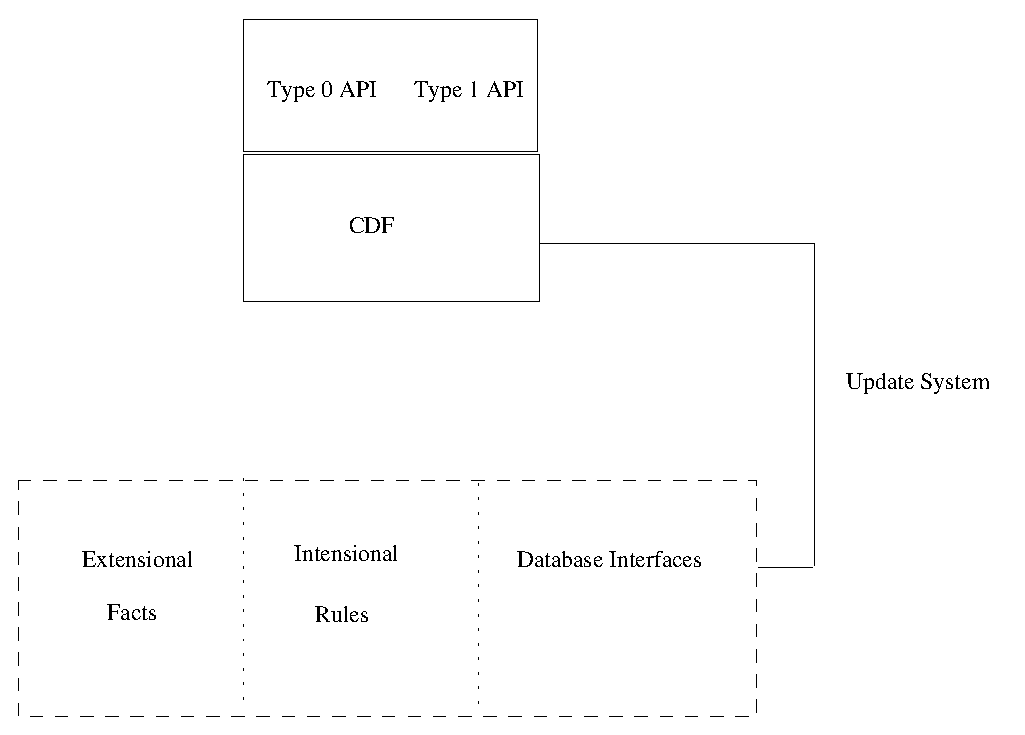
\epsfig{file=Figures/arch.eps,width=0.80\textwidth}}
%\caption{A High-Level Architecture of CDF and XJ}
%\label{fig:arch}
%\end{figure}
%--------------

CDF instances can be classified either as Type-0 or a Type-1, each of
which has its own interface.  Type-0 instances are useful for storing
large amounts of information; and consistency and implication in
Type-0 instances is computable in polynomial time.  Type-0 instances
describe classes by existential and universal relations, qualified
number restrictions, and relational hierarchies, but descriptions omit
negation and disjunction. Type-0 instances also support a direct
product construction for objects and classes.  
\comment{
These product classes and objects can be useful for representing
certain types of non-binary relations, and are particularly useful for
incorporating knowledge represented as RDF facts \cite{}.  }
Information in Type-0 CDF instances is tightly coupled to XSB's
query mechanism, and CDF ensures that only the most specific answers
(according to a given inheritance hierarchy) are returned for any
Type-0 query.

Type-1 instances extend Type-0 instances to describe classes using
negation and disjunction, and thus permit descriptions that are
equivalent to an expressive description logic.  In fact, a Type-1 CDF
instance can be seen as a knowledge base in which various classes are
described via {\em class expressions}, which correspond to formulas in
description logics.  Reasoning in Type-1 instances is done via the CDF
theorem-prover.  Using the Type-1 API, users may ask whether a given
class or object is consistent, whether a given class expression is
consistent with a class or object; or whether a given class expression
is entailed by a given class or object.  The problems of determining
consistency or entailment of a Type-1 class expression have a high
degree of complexity.  To solve these problems the CDF theorem prover
uses several heuristics, but a determined (or unlucky) user can always
find class expressions that requires a lot of time to check.

Of course, ontology management systems require many features in
addition to reasoning and representation features \cite{MGPS03}.  We
mention some of these features.

\begin{itemize}
\item {\em A Semantic Checking System}.  CDF has various mechanisms for
ensuring consistency of objects and classes both at the Type-0 or
Type-1 level.  Various levels of consistency can be checked during
various operations on the CDF instance.
%
\item {\em A Component System}. Reusability of ontologies is supported
by the {\em component} structure of CDF.  An ontology component may be
maintained by separate users or organizations in different locations
and assembled in various ways by applications.
%
\item {\em A Concurrency System}. (Not open-source) Based on the
component structure, the {\em concurrency} mechanism for CDF allows
users to update their own CDF instances and to periodically update a
common store. Naturally, the various mechanisms in CDF for ensuring
consistency that are vital to ensuring coherency when users update
their systems concurrently.
%
\item {\em Database Interfaces}. (Non open-souce) CDF supports various
interfaces to databases so that CDF facts can be stored in a database
or mapped to database tables.
\end{itemize}

Based on these features, CDF can support user interfaces in a number
of ways.  One of the most convenient is to use a XSB/Java interface
such as InterProlog~\cite{Cale01} or JAXSB~(see
\texttt{http://xsb.sourceforge.net}) and then write a user interface in
Swing or some other Java Graphics library.  One of the easiest ways to
do this is to make use of the {\em XJ system} which allows Swing Gui
objects to be represented as Prolog terms (the XJ system is non
open-source) From a systems perspective, a graphical interface is then
written XJ library Swing widgets or specialized XJ-CDF Swing widgets.
CDF per-se has the following graphical packages and applications.
%
\begin{itemize}
%
\item {\em An XJ Caching System}. Adds and deletes to CDF are extended
with a notification mechanism so that Java Swing objects (created with
XJ, XSB's graphics system) reflect the state of CDF even when it
dynamically changes.
%
\item {\em A Visual Editor}. Finally,  CDF supports a graphical editor
that allows users both to visualize an ontology and to perform the
functions mentioned so far.
\end{itemize}
%
Extensional facts, intensional rules, updates, the Type-0 and Type-1
interfaces, consistency checking predicates and the full component
system are available as an open-source package for XSB.  Other
features, concurrency mechanisms, specialized database interfaces, XJ
support and the editor are not yet open-source, but are included in
this manual to indicate the types of applications that can be
constructed with CDF.

%-----------------------------------------------------------
\section{The Meaning of Type-0 CDF Instances} \label{sec:type0} 

Facts in both Type-0 and Type-1 CDF instances are closely related to
class expressions in description logics.  However, because CDF often
stores class expressions as Prolog facts in an unconventional way, and
because description logics may not be familiar to a logic programming
audience, we present here a somewhat formal introduction to how CDF
represents knowledge.  Users without a mathematical background can
ignore the various axioms and formal definitions that are presented in
this chapter.  Our approach is to introduce a semantics of CDF based
on a translation of a {\em CDF instance} into a set of first-order
logic sentences that constitute an {\em Ontology Theory} whose models
are the models of a CDF instance.  For simplicity of presentation the
description of CDF instances in this section omits certain details
about components, extensional facts and intenstional rules, and other
topics that will be introduced in later chapters.

We illustrate aspects of CDF by means of an example drawn from
electronic commerce.  Health care organizations, such as hospitals,
clinics, etc., sometimes have difficulties in buying disposable
medical devices such as sutures, bandages, gloves, and so on.  These
difficulties arise from the fact that these devices may be quite
specialized: for instance some sutures are used only for particular
type of surgery on a particular organ.  At the same time, since these
devices are disposable, they may need to be purchased frequently.  We
consider concretely the class of {\em absorbable sutures}, which are
used for stitching and securing tissues, and which can be absorbed by
the human body.  Information below is adapted from he U.S. Defence
Logistics Information Service \url{http://www.dlis.mil}, from the
Universal Standard Products and Services Classification~\cite{UNSPSC},
as well as from websites of various commercial medical supply
companies.

\subsection{Type-0 CDF Instances} \label{sec:type0} 

We begin with the syntax of Type-0 instances~\footnote{The syntax for
  identfiers is simplified here, and differs in the actual CDF
  implementation. See Section~\ref{sec:instance}.}:

\begin{definition}[Type-0 Instances: Semantic Level] \label{def:ids}
A {\em Type-0 CDF instance} is a finite set of ground facts for the
predicates \pred{isa/2}, \pred{hasAttr/3}, \pred{allAttr/3},
\pred{classHasAttr/3}, \pred{minAttr/4}, and \pred{maxAttr/4}.  An {\em
identifier} is either a constant or a term.  The arguments of these
predicates are {\em concrete identifiers}, where a term $T$ is an
identifier iff $T$ has the functor symbol {\tt cid/1}, {\tt oid/1},
{\tt rid/1}, or {\tt crid/1} whose argument is either

\begin{enumerate}
\item a constant; or 
\item a term $f(I_1,\ldots,I_n)$ where $I_1,\ldots,I_n$ are identifiers.
\end{enumerate}
In the first case, an identifier is called {\em atomic}; in the second
it is called a {\em product identifier}.
\end{definition}

Despite the simple syntax of Type-0 CDF instances, their semantics
differs from the usual semantics assigned to facts in Prolog.
Identifiers identify sets of objects, or binary relations between
objects.  Furthermore, the facts of a Type-0 CDF instance can
implicitly denote inheritance of various relationships among classes
and objects, as well as inheritance constraints about what
relationships are allowed.

\subsection{Simple Taxonomies in CDF}

\begin{example} \rm \label{ex:suture1}
The following CDF instance illustrates a fragment of a taxonomy for
medical equipment.
%-------------------------------------------
{\tt  {\small 
\begin{tabbing}
foo\=foo\=foo\=foo\=foo\=foo\=foooo\=foooooooooooooooo\=\kill
isa(cid(medicalEquipment),cid('CDF Classes'))  \\
\> isa(cid(woundCareProducts),cid(medicalEquipment)) \\
\> \> \>  isa(cid(suturesAndRelatedProducts),cid(woundCareProducts)) \\
\> \> \> isa(cid(sutures),cid(suturesAndRelatedProducts))  \\
\> \> \> \> isa(cid(absorbableSutures),cid(sutures))  \\
\> \> \> \> isa(cid(nonAbsorbableSutures),cid(sutures)) \\
\> \\
\> \> \>   isa(oid(sutureU245H),cid(absorbableSutures))  \\
\> \> \> \> \>   isa(oid(suture547466),cid(sutures)) 
\end{tabbing} }} 
%-------------------------------------------
\noindent
In CDF, sets of objects are termed {\em classes} to stress the
informality of its sets from the perspective of set theory, and class
identifiers have the functor {\tt cid/1}.  One can read the fact
\begin{verbatim}
      isa(cid(nonAbsorbableSutures),cid(sutures))
\end{verbatim}
as ``all elements in the class {\tt cid(nonAbsorbableSutures)} are
also in the class {\tt cid(sutures)}'' --- in other words, that {\tt
cid(nonAbsorbableSutures)} is a subclass of {\tt cid(sutures)}.
Object identifiers have the functor {\tt oid/1}, and denote classes
with cardinality 1, or {\em singleton classes}.  The fact
\begin{verbatim}
      isa(oid(sutureU245H),cid(absorbableSutures))
\end{verbatim}
can be read as ``the element of the singleton class {\tt
oid(sutureU245H)} is in the class {\tt cid(absorbableSutures)}''.
Note that {\tt cid(absorbableSutures)} is (potentially) more specific
than the class {\tt cid(sutures)}, to which {\tt oid(suture547466)}
belongs.  The class {\tt cid('CDF Classes')} is taken to contain all
objects in the domain of discourse.  All identifiers in this simple
taxonomy are atomic.

The decision of whether to denote an entity as an object or as a class
depends on the use of a given CDF instance.  Here, a given part number
can specify a number of physical parts, but the physical parts are
taken to be identical for the purposes of this instance.  However, if
we were constructing a CDF instance for warehouse management, the
above objects might be better represented as classes, and the physical
objects represented as CDF objects.
\end{example} 

Implicit in the above example is the fact that we use the term {\em
object identifiers} or {\em objects} to denote singleton classes,
class identifiers to denote all classes (including singleton classes).
Elements cannot be denoted directly by CDF facts, but only through
singleton classes that contain them (and are isomorphic to them).  At
this point, we can begin defining the semantics of Type-0 CDF
instances.

%-------------------
\begin{definition} \label{def:ontolang}
\index{ontology language} \index{ontology structure} \index{ontology
theory}
%
An {\em ontology language} is a first-order language with equality
containing the predicates: {\em isClass/1, isElt/1, isRel/1, isCrel/1,
elt/2, rel/3, and crel/3}, and a countable set of constants.  An {\em
ontology structure} is a structure defined over an ontology language.
An {\em ontology theory} is a set of first-order sentences formed over
an ontology language that includes a set of {\em core axioms}, defined
below, along with the defined predicate:
\[
isObj(X) =_{def} isClass(X) \wedge 
	((elt(E_1,X) \wedge elt(E_2,X)) \Rightarrow E_1 = E_2)
\]
If $\cT$ is an ontology theory formed over an ontology
language $\cL$, an ontology structure $S$ over $\cL$ is a model of
$\cT$ if every sentence of $\cT$ is satisfied in $S$.
\end{definition}
%-------------------

\index{sorting predicates}
By convention we assume that the variables in an ontology language are
indexed by the set of natural numbers.  In this paper we will restrict
our attention to ontology languages whose constant and function
symbols are identifiers as described in Definition~\ref{def:ids}.
Informally $isClass/1$ indicates that an identifier $I$ is a class
name or {\em class identifier}; $isElt/1$ indicates that an identifier
$I$ is an element of a class; $isRel/1$ that $I$ is a {\em relation
identifier}; and $isCrel/1$ that $I$ is a {\em class-relation
identifier}; and $isObj/1$ that $I$ is an {\em object identifier}.  We
sometimes call these 5 predicates {\em sorting predicates}.
$elt(E,C)$ indicates that an element $O$ is a member of class
identifier $C$; $rel(O_1,R,O_2)$ indicates that an element $E_1$ has a
$R$ relation to an element $E_2$; and $crel(C_1,R,E)$ indicates that
the class identifier $C_1$ has a $R$ relation to an object identifier
$E$.

The first core axiom ensures that objects, classes, relations and
class-relations all have distinct identifiers within an ontology
language.
%-----------
\begin{axiom}[Distinct Identifiers] \label{ax:distinct}
\index{axioms!distinct identifiers} 
\ \\
\begin{tabbing}
foo\=foo\=foo\=foo\=foo\=foo\=foooo\=foooooooooooooooo\=\kill
\> $\neg \exists Id [isClass(Id) \wedge (isElt(Id) \vee isRel(Id) 
	                                 \vee isCrel(Id))] \wedge $ \\
\> $\neg \exists Id [isObj(Id) \wedge (isElt(Id) \vee isCrel(Id))] \wedge $ \\
\> $\neg \exists Id [isElt(Id) \wedge isCrel(Id)] $ 
\end{tabbing}
\end{axiom} 
%-----------

$isClass/1$, $isElt/1$, $isRel/1$, and $isCrel/1$ provide an effective
sorting that extends to all predicates, as the next axiom indicates.

\begin{axiom}[Predicate Sorts] \rm \label{ax:sorts}
\index{axioms!predicate sorts} 
\ \\
\begin{tabbing}
foo\=foo\=foo\=foo\=foo\=foo\=foooo\=foooooooooooooooo\=\kill
\> \> $(\forall X,Y) [elt(X,Y) \Rightarrow (isElt(X) \wedge isClass(Y))]
								\wedge $ \\
\> \> $(\forall X,Y,Z) [rel(X,Y,Z) \Rightarrow (isElt(X) \wedge isRel(Y)
					   \wedge isElt(Z))] \wedge  $ \\
\> \> $(\forall X,Y,Z) [crel(X,Y,Z) \Rightarrow (isClass(X) \wedge isRel(Y)
					   \wedge isElt(Z))] $ \\
\end{tabbing}
\end{axiom} 

%-----------

The following definition of $IdSort$ relates the functors of
identifiers in a Type-0 CDF instance to their sort in an ontology
theory.  It will be used in the various instance axioms to enforce
proper sorting of product identifiers.

\begin{definition}{\bf [IdSort]} \label{def:IdSort}
Let {\em I} is be an identifier. Then {\em IdSort(I)} is equal to {\em
isClass(I)} if the main functor symbol of {\em I} is {\tt cid/1}; {\em
isObj(I)} if the main functor symbol of {\em I} is {\tt oid/1}; {\em
isRel(I)} if the main functor symbol of {\em I} is {\tt rid/1}; and
{\em isCrel(I)} if the main functor symbol of {\em I} is {\tt crid/1}.
\end{definition}

%-----------------------------------------------------------------------------------------
\comment{
\begin{definition}{\bf [IdSort]}  Let {\em I} is be an identifier, and
$\cI$ be the set of identifiers occurring in {\em I}. Then
%
\[ IdSort(I) =_{def} \bigwedge_{I' \in \cI} Sort(I') \]
%
where {\em Sort(I)} is equal to {\em isClass(I)} if the main functor
symbol of {\em I} is {\tt cid/1}; {\em isObj(I)} if the main functor
symbol of {\em I} is {\tt oid/1}; {\em isRel(I)} if the main functor
symbol of {\em I} is {\tt rid/1}; and {\em isCrel(I)} if the main
functor symbol of {\em I} is {\tt crid/1}.
\end{definition}
}
%-----------------------------------------------------------------------------------------

From Definitions~\ref{def:IdSort} and~\ref{def:ontolang}, it is easy
to see that for any object identifier $O$, $IdSort(O) = isObj(O)$, and
$isObj(O) \Rightarrow isClass(O)$.

%-----------
\begin{instance} [Translation of {\tt isa/2}] \rm 
For each fact of the form {\tt isa(Id$_1$,Id$_2$)} add the axiom
\ \\
\begin{tabbing}
foo\=foo\=foo\=foo\=foo\=foo\=foooo\=foooooooooooooooo\=\kill
\> $ IdSort(Id_1) \wedge IdSort(Id_2) \wedge $ \\

\> \> $ (((isClass(Id_1) \wedge isClass(Id_2)) \wedge
	(\forall X) [elt(X,Id_1) \Rightarrow elt(X,Id_2)]) \vee $ \\

%\> \> $ ((isObj(Id_1) \wedge isClass(Id_2)) \wedge elt(Id_1,Id_2)) \vee $ \\

\> \> $ ((isRel(Id_1) \wedge isRel(Id_2)) \wedge
	(\forall X,Y)[rel(X,Id_1,Y) \Rightarrow rel(X,Id_2,Y)]) \vee $ \\

\> \> $ ((isCrel(Id_1) \wedge isCrel(Id_2)) \wedge
	(\forall X,Y)[crel(X,Id_1,Y) \Rightarrow crel(X,Id_2,Y)])) $ 
\end{tabbing}
denoted as {\tt isa(Id$_1$,Id$_2$)}$^{\cI}$.
\end{instance}
%-----------

Note that the reflexive and transitive closure of {\tt isa/2} is an
immediate consequence of its translation rule.  The next axiom is
technical.  It is important for the semantics of relations that each
class have at least one member.
%-----------
\begin{axiom}[Non-Empty Classes] \label{ax:nonnull}
\index{axioms!non-empty classes} 
\[ (\forall X) [isClass(X) \Rightarrow (\exists Y) [elt(Y,X)]] \]
\end{axiom} 
%-----------

The last core axiom for these predicates ensures is that each class is
a subclass of {\tt cid('CDF Classes')}.

%-----------
\begin{axiom}[Domain Containment] \label{ax:contained}
\index{axioms!domain containment} 
\[ (\forall X) [isElt(X) \Rightarrow elt(X,cid('CDF\ Classes'))] \]
\end{axiom} 
%-----------

\subsection{General Relations between Objects in  Classes}

\begin{example} \rm \label{ex:suture2}
The class {\tt cid(sutures)} can be further defined by its relations
to other classes.  For instance, an object in {\tt cid(sutures)} may
have a designation of its needle design indicating whether it is to be
used for abdominal surgeries, thoracic surgeries, or other purposes.
This information is indicated by the following CDF facts:
%
{\small
\begin{tabbing}
fooo\=foo\=foo\=foo\=fooooooooooooooooooooooooooooooo\=ooooooooooooo\=\kill
\> {\tt isa(rid(hasNeedleDesign),rid('CDF Relations'))} \\
\\
\> {\tt isa(cid(domainTypes),cid('CDF Classes'))} \\
\> \> {\tt isa(cid(needleDesignTypes),cid(domainTypes))} \\
\> \> \> {\tt isa(cid(Abdominal),cid(needleDesign))} \\
\> \> \> {\tt isa(cid(Abscisson),cid(needleDesign))} \\
\> \> \> {\tt isa(cid('Adson Dura'),cid(needleDesign))} \\
\> {\it \% 126 other values..}  \\
\\
\> {\tt allAttr(cid(sutures),rid(hasNeedleDesign),cid(needleDesign))} 
\end{tabbing}
}
%
\noindent
The {\tt allAttr/3} fact above can be read as ``if any object in {\tt
cid(absorbableSutures)} has a {\tt rid(hasNeedleDesign)} relation, it
must be to an object in the class {\tt cid(needleDesign)}''.  That
{\tt hasNeedleDesign} is a relation is indicated by clothing it in the
functor {\tt rid/1}.  This relation is an immediate subclass of all
{\tt CDF Relations} which in turn is taken to represent the universal
binary relation over the domain of discourse.  Thus the {\tt
allAttr/3} fact effectively types the range of {\tt
rid(hasNeedleDesign)} relations, stemming from objects in the class
{\tt cid(absorbableSutures)}, but it does not indicate the existence
of such a relationship.  From a user's point of view, the {\tt
rid(hasNeedleDesign)} relation can be thought of as an optional
attribute for a given {\tt cid(absorbableSutures)} object.  Sample
values for {\tt cid(hasNeedleDesignTypes)} are also given.
\end{example} 

%-------------------

{\tt allAttr/3} provides a simple but powerful mechanism for
inheritance of typing among CDF classes:
%---------------------------------------------------------------------------
\comment{
, as can be seen from the
following translation rule, which uses the defined formula

\[ 
elt(X,Y) =_{def} ((isClass(Y) \wedge elt(X,Y)) \vee (isObj(Y) 
			\wedge X = Y))
\] }
%---------------------------------------------------------------------------

\begin{instance} [Translation of {\tt allAttr/3}] \rm 
For each fact of the form {\tt allAttr(Id$_1$,Rid,Id$_2$)} add the instance
axiom: 
\begin{tabbing}
foo\=foo\=foo\=foo\=foo\=foo\=foooo\=foooooooooooooooo\=\kill
\> $ IdSort(Id_1) \wedge IdSort(Rid) \wedge IdSort(Id_2) \wedge $ \\
\> \> $ IsClass(Id_1) \wedge IsRel(Rid) \wedge IsClass(Id_2) \wedge $ \\
\> \> $(\forall X, Y) [(elt(X,Id_1) \wedge rel(X,Rid,Y))
					\Rightarrow elt(Y,Id_2)] $
\end{tabbing}
denoted as {\tt allAttr(Id$_1$,Rid,Id$_2$)$^{\cI}$}.
\end{instance}

%----------------------
\comment{
\begin{tabbing}
foo\=foo\=foo\=foo\=foo\=foo\=foooo\=foooooooooooooooo\=\kill
\> $ IdSort(Id_1) \wedge IdSort(Rid) \wedge IdSort(Id_2) \wedge $ \\
\> \> $ (IsClass(Id_1) \vee isObj(Id_1)) \wedge IsRel(Rid) \wedge 
	 (IsClass(Id_2) \vee isObj(Id_2)) \wedge $ \\
\> \> $(\forall X, Y) [(elt(X,Id_1) \wedge rel(X,Rid,Y))
					\Rightarrow elt(Y,Id_2)] $
\end{tabbing}
}
%----------------------
\begin{example} \rm \label{ex:hasAttr}
While {\tt allAttr/3} indicates a typing for relations, it does not
indicate that a relation must exist for elements of a class.  This
statement is made by \pred{hasAttr/3}.  The relation {\tt
rid(hasPointStyle)} for the class {\tt cid(absorbableSutures)} is
taken to be required in this schema.  The facts
%
{\small
\begin{tabbing}
fooo\=foo\=foo\=foo\=foooooooooooooooooooooooooooo\=ooooooooooooo\=\kill
\> {\tt allAttr(cid(absorbableSutures),rid(hasPointStyle),cid(pointStyle)) } \\
\> {\tt hasAttr(cid(absorbableSutures),rid(hasPointStyle),cid(pointStyle)) }
\end{tabbing}
}
%
\noindent
indicate not only the range of such relationships, but that such a
relationship must exist.  Indeed, the {\tt hasAttr/3} fact can be read
as ``all objects in the class {\tt cid(absorbableSutures)} have a
relation {\tt rid(hasPointStyle)} to an object in the class {\tt
cid(pointStyle)}''.  The facts below also give information about the
{\tt rid(hasPointStyle)} relation.
%
{\small
\begin{tabbing}
fooo\=foo\=foo\=foo\=foooooooooooboooooooooooooooo\=ooooooooooooo\=\kill
\> {\tt isa(cid(pointStyle),cid(domainTypes))} \\
\> {\tt isa(cid(regularCuttingEdge),cid(pointStyle))} \\
\> {\tt isa(cid(reverseCuttingEdge),cid(pointStyle))} \\
\> {\tt isa(cid(scalpelPoint),cid(pointStyle))} \\
\> {\it \% 10 other values.} \\
\\
\> {\tt hasAttr(oid(sutureU245H),rid(hasPointStyle),cid(regularCuttingEdge))}
\end{tabbing}
} 
\noindent
The last of the above facts can be read as ``the object {\tt
oid(sutureU245H)} has a {\tt rid(hasPointStyle)} relation to an object
in the class {\tt cid(pointStyle)}''.  
\end{example}

Not surprisingly, the definition of {\tt hasAttr/3} bears some
similarity to that of {\tt allAttr/3}.

\begin{instance} [Translation of \pred{hasAttr/3}] \rm 
For each fact of the form {\tt hasAttr(Id$_1$,Rid,Id$_2$)} add the instance
axiom: 
\begin{tabbing}
foo\=foo\=foo\=foo\=foo\=foo\=foooo\=foooooooooooooooo\=\kill
\> $ IdSort(Id_1) \wedge IdSort(Id_2) \wedge IdSort(Id_2) \wedge $ \\
\> \> $ IsClass(Id_1) \wedge IsRel(Rid) \wedge
	 IsClass(Id_2) \wedge $ \\
\> \> \> $ (\forall X) [elt(X,Id_1) \Rightarrow \exists Y [rel(X,Rid,Y) 
					\wedge elt(Y,Id_2)]]$
\end{tabbing}
denoted as {\tt hasAttr(Id$_1$,Rid,Id$_2$)$^{\cI}$}.
\end{instance}

We next turn to relational axioms that indicate the cardinality of
various relations.

\begin{example} \rm  \label{ex:maxAttr}
For our purposes, an object in {\tt cid(absorbableSutures)} can be
thought of as consisting of a needle and a thread~\footnote{The thread
is often called a suture.  We are assuming for purposes of
illustration that all sutures are --- in suture-speak --- ``armed''.}.  This is
represented by the facts:
%
{\small
\begin{tabbing}
foo\=foo\=foo\=foo\=foo\=foo\=foooo\=foooooooooooooooo\=\kill
\> {\tt allAttr(cid(absorbableSutures),rid(hasImmedPart),cid(absSutPart)) } \\
\> {\tt hasAttr(cid(absorbableSutures),rid(hasImmedPart),cid(absSutNeedle)) } \\
\> {\tt hasAttr(cid(absorbableSutures),rid(hasImmedPart),cid(absSutThread)) } \\
\\
\> {\tt isa(cid(absSutPart),cid(suturesAndRelatedProducts))}  \\
\> \> {\tt isa(cid(absSutNeedle),cid(absSutPart)) } \\
\> \> {\tt isa(cid(absSutSuture),cid(absSutPart)) } 
\end{tabbing}
}
%
\noindent
A needle for an absorbable suture is typically made of a different
material than the thread to which the needle is attached.  Each of
these materials may be important in choosing an absorbable suture, and
each of these materials are unique.  The facts
%
{\small
\begin{tabbing}
foo\=foo\=foo\=foo\=foo\=foo\=foooo\=foooooooooooooooo\=\kill
\> {\tt hasAttr(cid(absSutPart),rid(hasMaterial),cid(absSutMaterial)) } \\
\> {\tt maxAttr(cid(absSutPart),rid(hasMaterial),cid(absSutMaterial),1) } \\
\\
\> {\tt isa(cid(material),cid(domainTypes))} \\
\> {\tt isa(cid(absSutMaterial),cid(material)} \\
\> {\tt isa(cid(gut),cid(absSutMaterial))} \\
\> {\tt isa(cid(polyglyconate),cid(absSutMaterial))} \\
\> {\tt isa(cid(polyglyconicAcid),cid(absSutMaterial)) } 
\end{tabbing}
}
%
\noindent
indicate that each {\tt cid(absSutPart)} has a unique material.  The
{\tt maxAttr/4} fact can be read as ``Each object in the class {\tt
cid(absSutPart)} has at most 1 {\tt rid(hasMaterial)} relation to an
object in the class {\tt cid(absSutMaterial)}''.
\end{example}

In order to define the semantics of {\tt maxAttr/4}, let
$\exists^{\leq n}X_m[ \phi(X,Z)]$ be defined as an abbreviation for
the formula
\[
  \exists x_m,...,\exists x_{m+n} [\bigwedge_{m \leq i \leq m+n} 
	\phi(x_i,\overline{z}) 
	\Rightarrow \bigvee_{m \leq i < j \leq m+n} x_i  = x_j]
\]
i.e., for the formula indicating that there are at most $N$ non-equal
elements satisfying $\phi(x,z)$.  The abbreviation $\exists^{\geq N}$
is defined similarly to indicate that a formula is satisfied by at
least $N$ non-equal elements.

\begin{instance} [Translation of {\tt maxAttr/4}] \rm 
For each fact of the form {\tt maxAttr(Id$_1$,Rid,Id$_2$,N)} add the instance
axiom: 
\begin{tabbing}
foo\=foo\=foo\=foo\=foo\=foo\=foooo\=foooooooooooooooo\=\kill
\> $ IdSort(Id_1) \wedge IdSort(Id_2) \wedge IdSort(Id_2) \wedge $ \\
\> \> $ IsClass(Id_1) \wedge IsRel(Rid) \wedge
	 (IsClass(Id_2) \wedge $ \\
\> \> \> $ (\forall X) [elt(X,Id_1) \Rightarrow \exists^{\leq N} Y [rel(X,Rid,Y) 
					\wedge elt(Y,Id_2)]]$
\end{tabbing}
denoted as {\tt maxAttr(Id$_1$,Rid,Id$_2$,N)$^{\cI}$}.
\end{instance}

A corresponding predicate, {\tt minAttr/4} is used to indicate a
minimality restriction on a relation.  {\tt minAttr/4} is defined
similarly to {\tt maxAttr/4}, but using $\exists^{\geq N}$ rather than
$\exists^{\leq N}$.  Indeed, the predicate
%
{\small {\tt 
\begin{tabbing}
foo\=foo\=foo\=foo\=foo\=foo\=foooo\=foooooooooooooooo\=\kill
\> hasAttr(cid(absSutPart),rid(hasMaterial),cid(absSutMaterial)).
\end{tabbing}
} }
%
\noindent
could be replaced by the predicate
%
{\small {\tt 
\begin{tabbing}
foo\=foo\=foo\=foo\=foo\=foo\=foooo\=foooooooooooooooo\=\kill
\> minAttr(cid(absSutPart),rid(hasMaterial),cid(absSutMaterial),1).
\end{tabbing}
} }
%
\subsection{Class Relations}
Each of the predicates discussed so far are inheritable in their first
argument.  For instance, the fact
{\small {\tt 
\begin{tabbing}
foo\=foo\=foo\=foo\=foo\=foo\=foooo\=foooooooooooooooo\=\kill
\> hasAttr(cid(absSutPart),rid(hasMaterial),cid(absSutMaterial)).
\end{tabbing}
} } 
%
\noindent
implies that every subclass of {\tt cid(absSutures)} will have a
material in the class {\tt cid(absSutMaterial)}.  However, classes may
have relations that do {\em not} hold for their subclasses or members.
For instance, a finite set may have a given cardinality, but its
proper subsets will have a different cardinality.  Such relations are
termed {\em class relations}.

%-------------------
\begin{example} \label{ex:strel} \rm 
A practical example of a class relation comes from an application that
may be called part equivalency matching.  In this application, the
possible attributes for a class of parts are given various weights.
Two parts match if the sum of the weights of their attributes that
match are above a given threshold.  The weighting for the {\tt
cid(pointStyle)} of sutures might be given as:
%----------------------------------
{\small 
{\tt 
\begin{tabbing}
foo\=foo\=foo\=foo\=foo\=foo\=foooo\=foooooooooooooooo\=\kill
\> isa(cid(pointStyleWeight),cid('CDF Classes')) \\
\> \> isa(cid(highWeight),cid(pointStyleWeight)) \\
\> \> isa(cid(lowWeight),cid(pointStyleWeight)) \\
\\
\> classHasAttr(cid(sutures),crid(pointStyleWeight),cid(highWeight))
\end{tabbing}
} }
%----------------------------------
\noindent
The {\tt classHasAttr/3} fact can be read as ``the class {\tt
cid(sutures)} has a {\tt crid(pointStyleWeight)} relation to an object
in {\tt cid(highWeight)}.  Matching weights are made non-inheritable
via {\tt classHasAttr/3} because a weight may depend on a given
classification of a part.  For instance if a part were classified as a
{\tt cid(nonAbsorbableSuture)}, its {\tt cid(pointStyle)} might weigh
less (or more) for determining whether two sutures are equivalent.
\end{example}
%------------------
\begin{instance} [Translation of {\tt classHasAttr/3}] \rm 
For each fact of the form {\tt classHasAttr(Id$_1$,CRid,Id$_2$)} add the
instance axiom: 
\begin{tabbing}
foo\=foo\=foo\=foo\=foo\=foo\=foooo\=foooooooooooooooo\=\kill
\> $ IdSort(Id_1) \wedge IdSort(CRid) \wedge IdSort(Id_2) \wedge $ \\
\> \> $ IsClass(Id_1) \wedge IsCrel(CRid) \wedge isClass(Id_2) \wedge $ \\
\> \> \> $ (\exists X) [elt(X,Id_2) \wedge crel(Id_1,CRid,X)] $
\end{tabbing}
denoted as {\tt classHasAttr(Id$_1$,Rid,Id$_2$)$^{\cI}$}.
\end{instance}
%----------

\subsection{Product Classes}

The above predicates allow the definition of various named binary
relations between classes.  However, binary definitions can sometimes
be inconvenient to use.  For instance, in the part equivalency
matching example, (Example~\ref{ex:strel}), it may be desirable to
make explicit the weight of the match as an indication of the strength
of the match.  The weight could be made explicit by a series of
definitions
%-------------------------------------------
{\small 
{\tt 
\begin{tabbing}
foo\=foo\=foo\=foo\=foo\=foo\=foooo\=fooooooooooooooo\=\kill
\> allAttr(\cid{dlaPart},\rid{suturesRusMatch\_low},\cid{suturesRusPart}) \\
\> : \\
\> allAttr(\cid{dlaPart},\rid{suturesRusMatch\_high},\cid{suturesRusPart})
\end{tabbing}
} } 
%----------------------------------
\noindent
indicting that a given part has a match of weight {\em low} through
{\em high}.  However, for a scale with a large number of values,
defining matches in this way is time-consuming and prone to errors.
To address this, we first define a new class {\tt \cid{matchScale}}
containing as subclasses the various match levels.  We then combine
{\tt \cid{matchScale}} with the class {\tt \cid{suturesRusPart}} in a
product with a {\em product identifier}, as in the following fact
%-------------------------------------------
{\small 
{\tt 
\begin{tabbing}
foo\=foo\=foo\=foo\=foo\=foo\=foooo\=foooooooooooooooo\=\kill
 
allAttr(\cid{dlaPart},\rid{suturesRusMatch}, \\
\> \> \> \> \cid{partMach(\cid{suturesRusPart},\cid{matchScale})})
\end{tabbing}  } }
\noindent 
which indicates that a {\tt \cid{dlaPart}} can have a {\tt
\cid{suturesRusMatch}} to an object in the {\tt partMatch/2}  class,
which has both a {\tt \cid{suturesRusPart}} component and a {\tt
\cid{matchScale}} component.

%-------------------------------------------------------------------

We capture the intuition behind product classes through the following
axiom schemas.  The first indicates that product identifiers 
are constructed from {\em constituent identifiers} of the same sort.

\begin{axiom}[Downward Closure] \label{ax:downcl}
\index{axioms!downward closure}
\ \\
For each product identifier $\cid{f(x_1,\ldots,x_n)}$,
$\oid{f((x_1,\ldots,x_n)}$, $\rid{f(x_1,\ldots,x_n)}$, and
$c\rid{f((x_1,\ldots,x_n)}$ the following axiom is added,
\begin{tabbing}
foo\=foo\=foo\=foo\=foo\=foo\=foooo\=foooooooooooooooo\=\kill
\> $isClass(\cid{f(x_1,\ldots,x_n)}) \Rightarrow 
	isClass(x_1) \wedge \ldots \wedge isClass(x_n) $\\
\> $isObj(\oid{f(x_1,\ldots,x_n)}) \Rightarrow 
	isObj(x_1) \wedge \ldots \wedge isObj(x_n) $\\
\> $isRel(\rid{f(x_1,\ldots,x_n)}) \Rightarrow 
	isRel(x_1) \wedge \ldots \wedge isRel(x_n) $\\
\> $isCrel(\crid{f(x_1,\ldots,x_n)}) \Rightarrow 
	isCrel(x_1) \wedge \ldots \wedge isCrel(x_n) $
\end{tabbing}
\end{axiom}

With this axiom, along with the use of $IdType/1$ in the various
instance axioms, we will sometimes refer to a CDF identifier $I$ as a
class identifier if its outer functor is {\tt cid/1}, an object
identifier if its outer functor is {\tt oid/1} etc.  The next axiom
associates product classes with the objects they contain.

\begin{axiom}[Implicit Subclassing] \label{ax:implsc}
\index{axioms!implicit subclassing} 

\begin{enumerate}
\item For each product identifier $cid(f(x_1,\ldots,x_n))$ or 
$oid(f(x_1,...,x_n))$, the following axioms are added for $x_i, 1 \leq i
\leq n$:
\[
(\forall E) [(elt(E,y_i) \Ra elt(E,x_i)) \Ra \\
	(\forall E') [elt(E',f(x_1,...x_n))[x_i/y_i] \Rightarrow elt(E',f(x_1,...x_n))]]
\]

\item For each product identifier $rid(f(x_1,\ldots,x_n))$ the
following axioms are added for $x_i, 1 \leq i 
\leq n$:
\begin{tabbing}
foo\=foo\=foo\=foo\=foo\=foo\=foooo\=foooooooooooooooo\=\kill
\> $(\forall E_1,E_2) [(rel(E_1,y_i,E_2) \Ra rel(E_1,x_i,E_2)) \Ra$ \\
\> \> $(\forall E'_1,E'_2) [rel(E'_1,f(x_1,...x_n),E'_2)[x_i/y_i] \Ra rel(E'_1,f(x_1,...x_n),E'_2)]]$
\end{tabbing}
\end{enumerate}
\end{axiom}

%-------------------------------------------
\comment{
\begin{axiom}[Implicit Subclassing] \label{ax:implsc}
\begin{enumerate}
\item For each product identifier $\oid{f(x_1,\ldots,x_n)}$ the
following axiom is added:  
\[(\forall O) [elt(O,\cid{f(x_1,\ldots,x_n)})
	\Ra (O = \oid{f(y_1,\ldots,y_n)} \wedge 
  		  elt(y_1,x_1) \wedge \ldots \wedge elt(y_n,x_n))] \]

\item For each product identifier $\cid{f(x_1,\ldots,x_n)}$ and for
each atomic identifier $\cid{c}$ the following axiom is
added:
\[ (\forall C) 
   ([elt(\oid{f(x_1,\ldots,x_n)},C)] \Ra (C = \cid{f(y_1,\ldots,y_n)}
   \vee C = \cid{c})) \]
\end{enumerate}
\end{axiom}
}
%-------------------------------------------

\begin{example} \rm
Axiom~\ref{ax:downcl} simply states that identifier types cannot be
mixed within a product identifier.  For instance, if {\tt
\oid{matchLevelN}} is an object in the {\tt \cid{matchScale}},
then the identifier 

{\tt \cid{partMatch(\cid{suturesRusMatch},\oid{matchLevelN})}}

\noindent
is improperly formed.  On the other hand, if {\tt \oid{sutureU245H}} is in
the class {\tt \cid{suturesRusPart}}, then the identifier {\tt
\oid{partMatch(\oid{sutureU245H},\oid{matchLevelN})}} is a product
identifier that is also an object identifier.

Axiom~\ref{ax:implsc} also means that the inheritance relation of a
product class is partly determined by the inheritance relation of its
constituent elements.
\end{example}

\comment{
Core Axiom~\ref{ax:implsc} can be used either to set up equality
constraints on a model of a CDF instance, or it can be used to
determine which CDF instances have free models (as explained in the
next section).  The following example illustrates the first use.

\begin{example} \rm \label{ex:equality}
Suppose we have the CDF instance
{\small 
{\tt 
\begin{tabbing}
foo\=foo\=foo\=foo\=foo\=foo\=foooo\=foooooooooooooooo\=\kill
\> isa(\cid{a},\cid{f(a)}.
\end{tabbing} } } 
\noindent
By Core Axiom~\ref{ax:nonnull} (Non-empty Classes), {\tt \cid{a}} has
at least one element, which can be called {\tt \oid{a1}}.  By the
instance axiom for the above fact, {\em elt(\oid{a1},\cid{f(a)}}.  By
Core Axiom~\ref{ax:implsc}(1), it must be the case that 
%
\[ \oid{a1} = \oid{f(Y)} \wedge elt(Y,\cid{a}) \]
%
If we take $Y = \oid{a1}$, then this means that 
%
$ \oid{a1} = \oid{f(\oid{a1})} $
% 
so that the above fragment has a model $\cM$ with a single individual
(in the universe of $\cM$) to which all object identifiers are mapped,
and that has a $elt/2$ relation to each individual to which a class
identifier is mapped (among other models).
\end{example}
}

%\input{models}

\section{Implementation and System Features} \label{sec:impl}
%
In this section we describe how the CDF system implements the
semantincs of Section~\ref{sec:type0} , as well as many other features
for ontology management.  We begin by describing CDF identifiers,
facts, and rules in Section~\ref{sec:instance}.  The Type-0 query
interface, based on tabled resolution is described in
Section~\ref{sec:type0query}.  Section~\ref{sec:type0query} describes
the Type-1 API, which is based on the CDF therorem prover.  Update and
consistency predicates for CDF are described in
Section~\ref{sec:update}.  Section~\ref{sec:config} describes how to
configure CDF, along with predicates that allow the user to examine
aspects of the CDF state.  Section~\ref{sec:components} describes
basic I/O for CDF, along with a more sophisticated {\em component}
system that is built on top of basic I/O.  Section~\ref{sec:database}
describes database interfaces for CDF, and
Section~\ref{sec:concurrency} describes concurrency support.

%----------------------------------------------------


\subsection{CDF Instances} \label{sec:instance}

Part~\ref{part:semantics} simplified the syntax of CDF instances in
certain ways.  In this section we describe those aspects of the actual
CDF implementation that differ from the abstract presentation
Part~\ref{part:semantics}.

The first major difference concerns CDF identifiers.

\index{CDF Identifer}
\index{component tag}
\begin{definition}[CDF Identifiers] \label{def:cdfids}
A {\em CDF identifier} has the functor symbol {\tt cid/2}, {\tt
oid/2}, {\tt rid/2}, or {\tt crid/2}.  The second argument of a CDF
identifier is a Prolog atom and is called its {\em component tag},
while the first argument is either
\begin{enumerate}
\item a Prolog atom or 
\item a term $f(I_1,\ldots,I_n)$ where $I_1,\ldots,I_n$ are CDF identifiers.
\end{enumerate}
In the first case, an identifier is called {\em atomic}; in the second
it is called a {\em product identifier}.
\end{definition}

Thus in an implementation of, say, Example~\ref{ex:suture1} all
identifiers would have component tags.  For instance the identifier
{\tt cid(absorbableSutures)} might actually have the form {\tt
cid(absorbableSutures,unspsc)} and {\tt oid(sutureU245H)} would have
the form {\tt oid(sutureU245H,sutureRus)}.  These component tags have
two main uses.  First, they allow ontolgies from separate soruces to
be combined, and thus function in a manner somewhat analogous to XML
namespaces.  Second, the component tags are critical to the CDF
component system, described in \secref{sec:components}.

%----------------------------------------------------------------------------
\subsubsection{Extensional Facts and Intensional Rules}

\index{extensional facts} \index{intensional rules}
%
An actual CDF instance is built up of {\em extensional facts} and {\em
intensional rules} defined for the CDF predicates {\tt isa/2} {\tt
allAttr/3}, {\tt hasAttr/3}, {\tt classHasAttr/3}, {\tt coversAttr/3},
{\tt minAttr/4} and {\tt maxAttr/4}.  Extensional facts for these
predicates add the suffix {\tt \_ext} to the suffix name leading to
{\tt isa\_ext/2}, {\tt allAttr\_ext/2} and so on.  Intensional rules
add the suffix {\tt \_int} leading to {\tt isa\_int/2}, {\tt
allAttr\_int/2} etc.

Extensional facts make use of XSB's sophisticated indexing of dynamic
predicates.  Since CDF Extensional Facts use functors such as {\tt
  cid/1} or {\tt oid/1} to type their arguments, traditional Prolog
indexing, which makes use only of the predicate name and outer functor
of the first argument, is unsuitable for large CDF instances.  CDF
extensional facts use XSB's star-indexing (cf. Volume 1 of this
manual).  For ground terms, star-indexing can index on up to the first
five positions of a specified argument.  In addition, various
arguments and combinations of arguments can be used with star-indexing
of dynamic predicates.  The ability to index within a term is critical
for the performance of CDF; also since star-indexing bears
similarities to XSB's trie-indexing~\cite{RRSSW98}, it is spatially
efficient enough for large-scale use.  Section~\ref{sec:config}
provides information on default indexing in CDF and how it may be
reconfigured.

Intensional rules may be defined as XSB rules, and may use any of
XSB's language or library features, including tabling, database, and
internet access.  Intensional rules are called on demand, making them
suitable for implementing functionality from lazy database access
routines to definitions of primitive types.

\begin{example} \rm \label{ex:intrules}
In many ontology management systems, integers, floats, strings and so
on are not stored explicitly as classes, but are maintained as a sort
of {\em primitive type}.  In CDF, primitive types are easily
implemented via intensional rules like the following.
%
{\small {\sf  
\begin{tabbing}
foo\=foo\=foooooooooooooooooooooooooooooooooooooooo\=foo\=\kill
%
\> isa\_int(oid(Float),cid(allFloats)):- \\
\> \> 	(var(Float) -$>$ cdf\_mode\_error ; float(Float). \\
\end{tabbing} } }
\end{example}
%
CDF provides intensional rules defining all Prolog primitive types as
CDF primitive types in the component \component{cdfpt} (see below).
Other, more specialized types can be defined by users by defining
intensional rules along the same lines {\sc fill in 'below'; tabling
and intensional rules}

As mentioned above, the predicate {\tt
immed\_hasAttr/3}, (and {\tt immed\_allAttr/3}, etc) is used to store
basic CDF information that is used by predicates implementing {\tt
hasAttr/3} and other relations.  {\tt immed\_hasAttr/3} itself is
implemented as:
%
{\small {\sf  
\begin{tabbing}
foo\=foo\=foooooooooooooooooooooooooooooooooooooooo\=foo\=\kill
%
\> immed\_hasAttr(X,Y,Z):- hasAttr\_ext(X,Y,Z). \\
\> immed\_hasAttr(X,Y,Z):- hasAttr\_int(X,Y,Z). \\
\> immed\_hasAttr(X,Y,Z):- immed\_minAttr(X,Y,Z,\_). 
\end{tabbing} } }
%
\noindent
The above code fragment illustrates two points.  First, {\tt
immed\_hasAttr/3} is defined in terms of {\tt immed\_minAttr/3},
fulfilling the semantic requirements of Section \ref{sec:type0}.
It also illustrates that {\tt immed\_hasAttr/3} is implemented in
terms both of extensional facts {\tt hasAttr\_ext/3} and intensional
rules {\tt hasAttr\_int(X,Y,Z)}.  

%-------------------------------------------

\subsubsection{The Top-level Hierarchy and Primitive Types}

All CDF instances share the same top-level hierarchy, as depicted in
Figure~\ref{fig:toplevel}.  All classes and objects are subclasses
(through the {\tt isa} relation) to {\tt cid('CDF Classes',cdf)}, all
relations are subrelations of {\tt rid('CDF Object-Object
Relations',cdf)} and all class relations are subrelations of {\tt
crid('CDF Class-Object Relations',cdf)}.
%-------------------------------------------
\index{identifiers!cid('CDF Classes',cdf)}
\index{identifiers!rid('CDF Object-Object Relations,cdf)}
\index{identifiers!crid('CDF Class-Object Relations',cdf)}
\index{identifiers!cid('CDF Primitive Types',cdf)}
\index{identifiers!cid(allIntegers,cdf)}
\index{identifiers!cid(allFloats,cdf)}
\index{identifiers!cid(allAtoms,cdf)}
\index{identifiers!cid(allStructures,cdf)}
\index{identifiers!cid(atomicIntegers,cdf)}

\begin{figure}[htb] 
{\small {\it
\begin{center}
\begin{bundle}{cid('CDF Classes',cdf)}
\chunk{\begin{bundle}{cid('CDF Primitive Types',cdf)}
  \chunk{\begin{bundle}{cid(allIntegers,cdf)\ \ \ \ \ \    }
	\chunk{oid(Integer,cdfpt)}
	\end{bundle} }
  \chunk{\begin{bundle}{cid(allFloats,cdf)\ \ \ \ \ \ }
	\chunk{oid(Float,cdfpt)}
	\end{bundle} }
  \chunk{\begin{bundle}{cid(allAtoms,cdf)\ \ \ \ \ \ }
	\chunk{oid(Atom,cdfpt)}
	\end{bundle} }
  \chunk{\begin{bundle}{cid(allStructures,cdf)\ \ \ \ \ \ }
	\chunk{oid(Structure,cdfpt)}
	\end{bundle} }
  \chunk{\begin{bundle}{cid(atomicIntegers,cdf)}
	\chunk{oid(AInteger,cdfpt)}
	\end{bundle} }
  \end{bundle} } 
\end{bundle}
\end{center}

\ \\
\begin{center}
rid('CDF Object-Object Relations',cdf)
\end{center}

\ \\
\begin{center}
\begin{bundle}{crid('CDF Class-Object Relations',cdf)}
\chunk{crid('Name',cdf)}
\chunk{crid('Description',cdf)}
\end{bundle}
\end{center}
} }
\caption{Built-in Inheritance Structure of CDF}
\label{fig:toplevel}
\end{figure}
%-------------------------------------------

An immediate subclass of {\tt cid('CDF Classes',cdf)} is {\tt cid('CDF
Primitive Types',cdfpt)}.  This class allows users to maintain in CDF
any legally syntactic Prolog element, and forms an exception to
Definition~\ref{def:cdfids}.  Specifically {\tt cid('CDF Primitive
Types',cdf)} contains Prolog atoms, integers, floats, structures and
what are termed ``atomic integers'' --- integers that are represented
in atomic format, e.g. '01234'.  Primitive types are divided into five
subclasses, {\tt cid(allIntegers,cdf)}, {\tt cid(allFloats,cdf)}, {\tt
cid(allAtoms,cdf)}, {\tt cid(allStructures,cdf)}, and {\tt
cid(atomicInteger,cdf)}.  Each of these in turn have various objects
as their immediate subclasses~\footnote{Recall that objects in CDF are
singleton classes.}, whose inheritance relation is defined by an
intensional rule like the one presented in Example~\ref{ex:intrules}.
Thus, if the number 3.2 needs to be added to an ontology, perhaps as
the value of an attribute, it is represented as {\tt oid(3.2,cdfpt)},
and it will fit into the inheritance hierarchy as a subclass of {\tt
cid(allFloats,cdf)}.  The intensional rules are structured so that for
any Prolog syntactic element {\tt X}, when {\tt X} is combined with
the component \component{cdfpt}, then {\tt cid(X,cdfpt)} will be a
subclass of {\tt cid('CDF Primitive Types',cdfpt)}, as will be {\tt
oid(X,cdfpt)}.

\subsubsection{Basic CDF Predicates}

\begin{description}
\ourpredmodrptitem{isa\_ext/2}{usermod}
\ourpredmodrptitem{allAttr\_ext/3}{usermod}
\ourpredmodrptitem{hasAttr\_ext/3}{usermod}
\ourpredmodrptitem{classHasAttr\_ext/3}{usermod}
\ourpredmodrptitem{minAttr\_ext/4}{usermod}
\ourpredmodrptitem{maxAttr\_ext/4)}{usermod}
%\ourpredmodrptitem{coversAttr\_ext/3)}{usermod}
\ourpredmoditem{necessCond\_ext/2)}{usermod}
%
These dynamic predicates are used to store extensional facts in CDF.
They can be called directly from the interpreter or from files that
are not modules, but must be imported from {\tt usermod} by those
files that are modules.  Extensional facts may be added to a CDF system
via \pred{newExtTerm/1} (\secref{sec:update}), or imported from a
\ttindex{cdf\_extensional.P} file (\secref{sec:components}).

\ourpredmodrptitem{isa\_int/2}{usermod}
\ourpredmodrptitem{allAttr\_int/3}{usermod}
\ourpredmodrptitem{hasAttr\_int/3}{usermod}
\ourpredmodrptitem{classHasAttr\_int/3}{usermod}
\ourpredmodrptitem{minAttr\_int/4}{usermod}
\ourpredmodrptitem{maxAttr\_int/4)}{usermod}
%\ourpredmodrptitem{coversAttr\_int/3)}{usermod}
\ourpredmoditem{necessCond\_int/2)}{usermod}
%
These dynamic predicates are used to store intensional rules in CDF.
They can be called directly from the interpreter or from files that
are not modules, but must be imported from {\tt usermod} by those
files that are modules.  Intensional rules may be added to a CDF
system via \pred{???newIntRule/1} (\secref{sec:update}), or imported from
a \ttindex{cdf\_intensional.P} file (\secref{sec:components}).


\ourpredmoditem{immed\_isa/2}{cdf\_init\_cdf}
{\tt immed\_isa(SubCid,SupCid)} is true if there is a corresponding
fact in \pred{isa\_ext/2} or in the intensional rules.  It does not
use the Implicit Subclassing Axiom \ref{ax:implsc}, the Domain
Containment Axiom~\ref{ax:contained}, or reflexive or transitive
closure.

\ourpredmodrptitem{immed\_allAttr/3}{cdf\_init\_cdf}
\ourpredmodrptitem{immed\_hasAttr/3}{cdf\_init\_cdf}
\ourpredmodrptitem{immed\_classHasAttr/3}{cdf\_init\_cdf}
\ourpredmodrptitem{immed\_minAttr/4}{cdf\_init\_cdf}
\ourpredmodrptitem{immed\_maxAttr/4)}{cdf\_init\_cdf}
%\ourpredmodrptitem{immed\_coversAttr/3)}{cdf\_init\_cdf}
\ourpredmoditem{immed\_necessCond/2)}{cdf\_init\_cdf}
Each of these predicates calls the corresponding extensional facts for
the named predicate as well as the intensional rules.  No inheritance
mechanisms are used, and any intensional rules unifying with the call
must support the call's instantiation pattern.


\ourpredmoditem{cdf\_id\_fields/4}{cdf\_init\_cdf}
{\tt cdf\_id\_fields(ID,Functor,NatId,Component)} is true if {\tt ID}
is a legal CDF identifier, {\tt Functor} is its main functor symbol,
{\tt NatId} is its first field and {\tt Component} is its second
field.  This convenience predicate provides a faster way to examine
CDF identifiers than using {\tt functor/3} and {\tt arg/3}.

\end{description}

`\section{The Type-0 Query Interface} \label{sec:type0query}

There are two main design goals behind the Type-0 query interface.
\begin{itemize}
\item to provide a Prolog interface to CDF based on  
the axioms in Chapter~\ref{sec:type0}, and the {\sc inh} proof system
derived from \refsec{sec:inheritance} along with
Proposition~\ref{prop:necesscondinh}.
\item to provide a highly efficient and scalable interface to CDF.
\end{itemize}

Indeed, the Type-0 interface has been used to support CDF instances
containing nearly a million extensional facts that require heavy
manipulation and access, and are used as back-ends to interactive
graphical systems.  As discussed below, this need for efficiency
affects certain aspects of the interface.

\subsection{Virtual Identifiers}
As discussed, Type-0 instances do not make contain facts of the form
\pred{necessCond/2}.  In the implementation of CDF, {\tt necessCond/2}
goals can be called, and their implementation obeys the first-argument
inheritance for {\tt necessCond}.  However, it is important to note
that {\bf the Type-0 interface does not use information in virtual
identifiers} as the following example shows.

\begin{example} \rm 
Consider the CDF instance containing only the fact
{\small 
{\tt 
\begin{tabbing}
foo\=foo\=foo\=foo\=foo\=foo\=foooo\=foooooooooooooooo\=\kill
\> necessCond\_ext(cid(a,test),vid(exists(rid(r,test),cid(b,test)))).
\end{tabbing} } } 
%
\noindent
by the semantics of type 1 ontologies, this CDF instance logically
entails {\small {\tt
\begin{tabbing}
foo\=foo\=foo\=foo\=foo\=foo\=foooo\=foooooooooooooooo\=\kill
\> hasAttr(oid(a,test),rid(r.text),cid(b,text))$^{\cI}$
\end{tabbing} } } 
%
\noindent
However the Type-0 interface will answer ``no'' to the query 
{\small 
{\tt 
\begin{tabbing}
foo\=foo\=foo\=foo\=foo\=foo\=foooo\=foooooooooooooooo\=\kill
\> ?- hasAttr(oid(a,test),rid(r.text),cid(b,text)).
\end{tabbing} } } 
%
\end{example}

\subsection{Computing Irredundant Answers}

Consider the running sutures example of Chapter~\ref{sec:type0} to
which is added a fact
%
{\small 
{\tt 
\begin{tabbing}
foo\=foo\=foo\=foo\=foo\=foo\=foooo\=foooooooooooooooo\=\kill
\> hasAttr(oid(sutureU245H),rid(needleDesign),cid('Adson Dura')).
\end{tabbing} } } 
%
\noindent
Suppose the query {\tt ?-
hasAttr(oid(sutureU245H),rid(needleDesign),Y)} were asked.  Via an
{\sc inh} proof, rhe CDF instance would imply the answers 
%
{\small {\tt
\begin{tabbing}
foo\=foo\=foo\=foo\=foo\=foo\=foooo\=foooooooooooooooo\=\kill
\>  hasAttr(oid(sutureU245H),rid(needleDesign),cid('Adson Dura')) \\
\> hasAttr(oid(sutureU245H),rid(needleDesign),cid(needleDesignTypes)) \\
\>  hasAttr(oid(sutureU245H),rid(needleDesign),cid('CDF Classes))
\end{tabbing} } }
%
\noindent
The last two answers are, of course, redundant according to
Definition~\ref{def:redund}.  Omitting redundant answers is important
both for human comprehension of information in a CDF instance, and to
reduce excessive backtracking in applications.

% TLS coversAttr
Computation of irredundant answers is done in CDF by creating a {\em
preference relation}\ \ on the relations {\tt hasAttr/3}, {\tt
classHasAttr/3}, {\tt allAttr/3}, {\tt minAttr/3}, {\tt maxAttr/3} and
{\tt necessCond} using the techniques of \cite{CuSw02}.  The schematic
code for a query to {\tt hasAttr/3} in which the first argument is
known to be bound, and the second two free, is shown in
Figure~\ref{fig:preference}.  Basic information concerning {\tt
hasAttr/3} within a CDF instance is kept via the predicate {\tt
immed\_hasAttr/3} (and similarly for other CDF relations), and {\tt
hasAttr/3} uses {\tt immed\_hasAttr/3} to compute implications via
inheritance upon demand.  In the compilation of the code in
Figure~\ref{fig:preference}, well-founded negation is used to ensure
that only preferred answers are returned.  It is easy to see by
comparing the preference rules of Figure~\ref{fig:preference} with
Propositions~\ref{prop:inh1}-\ref{prop:inh2}, that the preference rule
ensures that answers are returned only if they are not implied by
other answers.  Similar approaches are used for other query modes and
CDF relations.  

\begin{figure}[htb] 
%-------------------------------------------
{\small {\sf  
\begin{tabbing}
foo\=foo\=foooooooooooooooooooooooooooooooooooooooo\=foo\=\kill
%
\> hasAttr(X,Y,Z):- \\
\> \> 	nonvar(X), \\
\> \> 	(var(Y) -$>$ hasAttr\_bff(X,Y,Z) ; hasAttr\_bbf(X,Y,Z)). \\
	   \\
\> :- table hasAttr\_bbf/3. \> \> :- table hasAttr\_bff/3.\\
\> hasAttr\_bbf(X,Y,Z):-  \> \> hasAttr\_bff(X,Y,Z):-  \\
\> \> 	isa(X,XSup), 	\> \> 	isa(X,XSup), \\
\> \> 	isa(Y,YSup), 	\> \>  	immed\_hasAttr(XSup,Y,Z). \\
\>  \> 	immed\_hasAttr(XSup,YSup,Z). \\
\\
\> prefer(hasAttr\_bbf(X,y,Z1),hasAttr\_bbf(X,Y,Z2)):-  
\> \> prefer(hasAttr\_bff(X,Y1,Z1),hasAttr\_bff(X,Y2,Z2)):-  \\
\> \> 	isa(Z1,Z2),\pnot(Z1 = Z2). 
\> \> 	isa(Y1,Y2),\pnot(Y1 = Y2), \\
\> \> \> \> 	isa(Z1,Z2),\pnot(Z1 = Z2).
%
\end{tabbing} } }
\caption{Schematic Representation for Selected Modes of {\tt
hasAttr/3} Implementation} 
\label{fig:preference}
\end{figure}

\subsection{Implementations of {\tt isa/2}} \label{sec:isaimpl}

In implementing {\tt isa/2} there are a number of tradeoffs to be made
between semantic power and efficiency.  We discuss some of them here
in order to motivate the design of the Type-0 API.

\subsubsection{To Table or Not to Table}  Tabling {\tt isa/2} (or the
predicates that underly it) may have several advantages.  First,
consider the goal {\tt ?- isa(cid('CDF Root',cdf),X)} that traverses
through the entire {\tt isa/2} hierarchy.  Is {\tt isa/2} is tabled,
{\tt X} will be instantiated once for each class in the hierarchy.  If
{\tt isa/2} is not tabled, {\tt X} will be instantiated for every path
in the hierarchy whose initial class is {\tt cid('CDF Root',cdf)}.
Since the number of paths in a directed graph can be exponential in
the number of nodes in the graph, a failure to table {\tt isa/2} can
potentially be disasterous.  Whether it is or not depends on the
structure of the inheritance hierarchy.  To the extent the hierarchy
is tree-like, tabling {\tt isa/2} will not be of benefit, as the
number of paths from any node in a tree is equal to the number of
nodes in the tree.  Indeed, in such a case, tabling {\tt isa/2} could
be a disadvantage, as large parts of the hierarchy may need to be
materialized in a table.  On the other hand, if there is much multiple
inheritance in the hierarchy, tabling {\tt isa/2} can vastly improve
performance.
%
A second consideration is whether intensional rules are used in a CDF
instance, and if so, the form of the rules.  If intensional rules
themselves call predicates in the Type-0 interface, there is a risk of
infinite loops if {\tt isa/2} isn't tabled.

As a result of these considerations, certain predicates underlying
{\tt isa/2} are tabled.  However, this tabling can be removed by
reconfiguring and recompiling CDF.  To do this, the file {\tt
cdf\_definitions.h} in {\tt \$XSBHOME/packages/altCDF} must be edited,
changing the line

{\tt DEFINE TABLED\_ISA 1}

\noindent to

{\tt DEFINE TABLED\_ISA 0}

\noindent
and recompiling {\tt cdf\_init\_cdf.P}.

\subsubsection{Product Classes}
%
From an operational perspective however, a query @tt{?- isa(X,Y)} can
easily be intractable if product classes are used.

\begin{example} \rm
Let {\tt cid(boolean,s)} be a class with two subclasses: {\tt
oid(true,s)} and {\tt oid(false,s)}.  Then the product class {\tt
cid(f(cid(boolean,s),...,cid(boolean,s),s)} will contain a number of
subclasses exponential in the arity of {\tt f}.
\end{example}

In order to use product classes in practical applications the
implementation of {\tt isa/2} distinguishes a general isa relation in
which a given fact may be proved using Instance Axioms, the Domain
Containment Axiom (Axiom~\ref{ax:contained}) and the Implicit Isa
Axiom (Axiom~\ref{ax:implsc}) from {\em explicit} isa proved without
the Implicit Subclassing Axiom.  Based on this distinction, two
restrictions are made:

\begin{enumerate}

\item {\em Restriction 1}: Axioms used to prove answers to the query
{\tt ?- isa(X,Y)} depend on the instantiation of {\tt X} and {\tt Y}.

\item {\em Restriction 2}: If {\tt immediate\_isa(Id1,Id2)} is true then
{\tt Id2} is an atomic identifier.
\end{enumerate}

We discuss each restriction in turn.  The behavior of {\tt isa/2} for
various instantiation patterns is as follows.

\begin{enumerate} 

\item If {\tt Id1} and {\tt Id2} are both ground, the Implicit
Subclassing Axiom is used, if necessary.

\item If {\tt Id1} is not ground, the Implicit Subclassing Axiom is
{\em not} used, in order to avoid returning a number of answers that
is exponential in the size of a product identifier.

\item If {\tt Id1} is ground but not {\tt Id2} then the Implicit
Subclassing Axiom may used in the first step of a derivation.  In
other words, in any isa derivation for this instantiation pattern, the
first step may use the Implicit Subclassing Axiom to "match" a term in
the {\tt immediate\_isa/2} relation, but subsequent steps must use
explicit isa.  Upon backtracking the Implicit Subclassing Axiom may be
used again to begin a new derivation, but subsequent steps in this
derivation must cannot use this axiom.
\end{enumerate}

The second assumption helps to reinforce the assumption of case 3
above.  Without it, users might expect that the Implicit Subclassing
Axiom could be used in each step of a derivation of an {\tt isa/2}
fact.  Such an implementation would slow down the execution of {\tt
isa/2} so that it would be unusable for many
applications~\footnote{Given Restriction 2, atomic identifiers usually
occur within the inner loops of {\tt isa/2}.  Atomic identifiers have
the advantage that these inner loops can use unification to traverse
the hierarchy.  If product identifers are used, they must be
abstracted using {\tt functor/3} and the hierarchies of their inner
arguments traversed, a much slower method.}.

\begin{example}  \rm Suppose we have the following CDF instance.

{\small {\tt
\begin{tabbing}
foo\=foo\=foooooooooooooooooooooooooooooooooooooooo\=foo\=\kill
%
\> isa\_ext(cid(bot,s),cid(mid,s)). \\
\> isa\_ext(cid(mid,s),cid(top,s)). \\
\\
\> isa\_ext(cid(prod(cid(mid,s),cid(top,s)),s),cid(myClass,s)).
\end{tabbing} } }

\begin{itemize}
%
\item The query 
{\small {\tt
\begin{tabbing}
foo\=foo\=foooooooooooooooooooooooooooooooooooooooo\=foo\=\kill

\> ?- isa(cid(prod(cid(bot,s),cid(mid,s)),s),cid(prod(cid(mid,s),cid(mid,s)),s)
\end{tabbing} } }

would succeed.

\item 
{\small {\tt
\begin{tabbing}
foo\=foo\=foooooooooooooooooooooooooooooooooooooooo\=foo\=\kill

\> ?- isa(cid(prod(cid(bot,s),cid(mid,s)),s),X)
\end{tabbing} } }
would successively unify {\tt X} with 
{\small {\tt
\begin{tabbing}
foo\=foo\=foooooooooooooooooooooooooooooooooooooooo\=foo\=\kill
\> (1) cid(prod(cid(bot,s),cid(mid,s)),s), \\
\> (2) cid(prod(cid(mid,s),cid(top,s)),s), \\
\> (3) cid(myClass,s), {\rm and} \\
\> (4) cid('CDF Root',cdf)
\end{tabbing} } }

\item The query
{\small {\tt
\begin{tabbing}
foo\=foo\=foooooooooooooooooooooooooooooooooooooooo\=foo\=\kill

\> ?- isa(X,cid(prod(cid(mid,s),cid(mid,s)),s))
\end{tabbing} } }
would unify {\tt X} only with {\tt
cid(prod(cid(mid,s),cid(mid,s)),s)}

\end{itemize}
\end{example}

\subsection{The Type-0 API} \label{sec:type0api}

Exceptions to all predicates in this API are based on the context {\tt
query} (See \refsec{sec:consist}).

\begin{description}

%----------------------------------------------------------------
\comment{
\ourpreditem{implicit\_isa/2}  {\tt implicit\_isa(Id1,Id2)} forms a partial
implementation of the Implicit Subclassing Axioms for product
identifiers\ref{???}.  As an example of implicit isaing of product
classes, {\tt id(f(id(a,source1),id(b,source2),source3)} is a subclass
of {\tt id(f(id(c,source1),id(b,source2),source3)} if {\tt
id(a,source1)} is a subset of {\tt id(a,source1)}.  Because the use of
product identifiers can isa relations that are exponential in the size
of the product identifiers, the implementation described below
attempts to partially traverse the implicit isa relation in a manner
that is semantically meaningful while also remaining tractable.

The semantics of {\tt implicit\_isa/2} is mode-dependent.  Let fully
ground inputs be treated as {\tt +} and non-fully ground inputs treated
as {\tt -}.  Suppose we have a call {\tt implicit\_isa(C1,C2)}:

\begin{itemize} 
\item {\tt implicit\_isa(+,+)}: succeeds if {\tt C1} is
not equal to {\tt C2} and {\tt C1} is lower than {\tt C2} on the isa
hierarchy by the isa axioms.

\item {\tt implicit\_isa(+,-)}: succeeds if {\tt C1} \=
{\tt C2}, {\tt C1} is a subclass, (member, etc) of {\tt C2} by the isa
axioms {\em and} for some {\tt C3} {\tt immed\_isa(C2,C3)} is true.

\item {\tt implicit\_isa(-,+)}: fails.

\item {\tt implicit\_isa(-,-)}: fails.
\end{itemize}

The motivation for this partial implementation is as follows.  If both
terms are ground, determining their relation in the isa hierarchy is
linear in the sizes of the terms.  In all cases where variables are
present, there is the possibility of backtracking through a large
isa\_relation.  For the instantiation pattern {\tt immed\_isa(+,-)}
this is addressed by searching through only those product identifiers
that occur in the first argument of the immediate isa relation.
Because of the assumption that product identifiers can occur only in
the first argument of the immediate isa relation, this option is not
available for the instantiation patterns {\tt implicit\_isa(-,+)} and
{\tt implicit\_isa(-,-)}, so they fail. }
%----------------------------------------------------------------

\ourpredmoditem{isa/2}{cdf\_init\_cdf} The operational semantics of
{\tt isa/2} is defined in \refsec{sec:isaimpl}.

\comment{
/* TLS: the supporting predicates for isa/2 may or may not be tabled.
Certain of the CDF operations depend on the prolog semantics of isa.
Rather than changing these predicates, I moved isa tabling to a lower
level, past mode checks, and the first call to isa in each mode.  This
should cause no extra tabling beyond tabling isa/2, and perhaps a bit
less tabling.  If you definately want tabled behavior use
table\_isa/2.  Note that explosive\_isa/2, proper\_isa/2*/}

\ourpredmoditem{explosive\_isa/2}{cdf\_init\_cdf}
{\tt explosive\_isa(Sub,Sup)} follows the isa axioms for product
identifiers rather than the algorithm of {\tt isa/2}. Thus if neither
{\tt Id1} nor {\tt Id2} are product identifiers, or if {\tt Id1} and
{\tt Id2} are fully ground product identifiers, {\tt explosive\_isa/2}
behaves as {\tt isa/2}.  Otherwise, suppose {\tt Id1} is a (perhaps
partially ground) product identifier whose Nid has the outer functor
{\tt F/A}.  If the Nid of {\tt Id2} is a variable, it is instantiated
to a skeleton of {\tt F/N}; otherwise its outer functor must be {\tt
F/A}.  In either case, both Nids are broken into their constituent
identifiers and {\tt explosive\_isa/2} is recursively called on each
of these.  {\tt explosive\_isa/2} thus removes Restriction 1 above,
but not Restriction 2.

\ourpredmodrptitem{allAttr/3}{cdf\_init\_cdf}

\ourpredmodrptitem{hasAttr/3}{cdf\_init\_cdf}

\ourpredmodrptitem{maxAttr/4}{cdf\_init\_cdf}

\ourpredmodrptitem{minAttr/4}{cdf\_init\_cdf}

\ourpredmoditem{classHasAttr/3}{cdf\_init\_cdf}
%
These predicates assume they are operating on a CDF instance, $\cO$ in
which the {\tt isa/2} relation is acyclic.  For efficiency reasons,
given a goal, $G$, the behavior of these predicates further depends on
whether various arguments of $G$ are ground atomic identifiers. 
\begin{itemize}
\item  If either the first argument of $G$ is a ground atomic
identifier, or the second and third arguments of $G$ are ground atomic
identifiers, each answer $G\theta$ will be a member of a set $S$ which
is the most specific irredundant set containing only elements that
unify with $G$.
%
\item Otherwise, each answer $G\theta$ will be a member of a set $S$ that 
is the most specific irredundant set containing only elements that
unify with $G$.
\end{itemize}


\ourpredmoditem{nessesCond/2}{cdf\_init\_cdf}
Given a goal {\tt nessesCond(?Id,-Vid)}, each answer
$nessesCond(Id,Vid)\theta$ will be a member of a set $S$ which is the
most specific irredundant set containing only elements that unify with
{\tt nessesCond(?Id,-Vid)}.  

\ourpreddomitem{isType0Term/1}{cdf\_checks}
{\tt isType0Term(?Term)} succeeds if {\tt Term} unifies with an
extensional fact (e.g. a term of the form {\tt isa\_ext(A,B)}, {\tt
hasAttr\_ext(A,B)}, etc.), an intensional rule head (e.g. a term of
the form {\tt isa\_int(A,B)}, {\tt hasAttr\_int(A,B)}, etc.), or a
semantic type-0 predicate (e.g. a term of the form {\tt isa(A,B)},
{\tt hasAttr(A,B)}, etc.).

\end{description}

%TLS: check out loops in hasAttr.

\section{The Type-1 API} \label{sec:type1query}

The Type-1 interface is radically different than the Type-0 interface.
While the Type-0 interface uses tabling and logical preferences to
return correct answers according to the {\sc inh} proof system, it is
still resolution-based.  However, when the disjunction and negation of
virdual identifiers is added such an approach is no longer possible,
so that the Type-1 query interface is based on computing logican
consistency and entailment.  Since logical entailment of class
expressions can be reduced to consistency, the Type-1 interface is
based on consistency checking of CDF instances that have been
transformed into class expressions.

Consistency checking of class expressions such as those of
Definition~\ref{def:ce} is decidable, but {\em P-space}
complete~\footnote{Assuming a linear encoding of the integers in the
{\em atLeast} and {\em atMost} constructs.  Formally, the CDF prover
is complete for ${\cal ALCQ}$ description logics extended with
relational hierarchies and product classes.}, so that determening
whether a Type-1 instance has a model requires radically different
checking techniques than Type-0 instances.  Query answering for Type-1
instances is performed by using theorem proving techniques.

\subsection{The CDF Theorem Prover}

Specialized theorem-provers are generally implemented to check
consistency of class expressions.  These provers may use based on
structural subsumption techniques (e.g. as used in
CLASSIC~\cite{PMBRB91}, LOOM~\cite{MacB94} and GRAIL~\cite{RBGHNS97});
tableaux construction~\cite{HoPS99}; or stable model
generation~\cite{Swif04} --- in \version{} of CDF a tableaux-style
prover is used.

At a high level, the CDF prover first translates a class expression
$CE$ to a formula $\psi$ in an ontology language according to
Definition~\ref{def:fot}.  It then attempts to construct a model for
$\psi$: if it succeeds $CE$ is consistent, otherwise $CE$ is
inconsistent (since the prover can be shown to be complete).  The CDF
prover has access to the relational and class hierarchies of a CDF
instance during its execution.  As a result, only the principle
classes and relations of an identifier (Definition~\ref{def:redund})
need be entered in class expressions.  Finally, since objects in the
semantics of CDF are indistinguishable from singleton sets, an object
identifier $O$ can be used in any context that a class identifier can
be used.  The prover takes accont of this by enforcing a cardinality
constraint for the set $O$.

The theorem prover of \version{} uses exhaustive backtracking, rather
than the dependency-directed backtracking that is typical of recent
provers such as the DLP prover \cite{}, the FaCT prover \cite{} or the
Racer prover \cite{}.  As a result, the CDF prover may be slow for
certain types of queries relative to these other provers.
Dependency-directed backtracking has not been added to the CDF prover
largely to keep it simple enough to experiment with different
extensions to the types of class expressions it supports~\footnote{In
particular, work is underway on extending the CDF prover to handle
functional attribute chains and concrete domains (see \cite{}).}.  On
the other hand, the CDF prover is relatively efficient on how it
traverses a CDF instance to check consistency.

When a CDF Type-1 instance is checked, the instance is translated into
either a class expression before it can be sent to the CDF prover.
Due to the high worst-case complexity of consistency checking, input
strings to the prover should be kept as small as possible.  The CDF
system accomplishes this by translating information about a given CDF
identifier into a series of local class expressions
(\refsec{sec:lce}), sending a local class expresion to the CDF prover,
then producing and checking other local class expressions as needed.
Since CDF instances differ in philosophy from terminological systems,
they may be expected to be cyclic, so that a given class identifier
may occur in a level $n$ local class expression of itself.

\subsection{The Type-1 API}

\begin{description}

\ourpreditem{checkIdConsistency/1}{cdftp\_chkCon}
In {\tt checkIdConsistency(IdList)} {\tt IdList} is a (list of) class
or object identifier(s) which is taken as a conjunction.  The
predicate succeeds if {\tt IdList} is consistent in the current CDF
instance.

{\bf Exceptions} {\tt Domain Exception: IdList} is not a class
identifier, an object identifier, or a list of class or object
identifiers.

%-----------------------------------------------------------------------------
\comment{
/* The algorithm is described in detail in the CDF system paper.  What
we do here is to prove consistency of an identifier by an iterative
process.  Given an identifier {\tt Id}, a local class expression is
constructed for Id, and a consistency check made for that class
expression.  In other words, we prove the consitency of Id by trying
to construct a model in which Id is a non-empty set if it is a cid, or
a non-empty unique set if Id is an oid.

Local class expressions dont contain all information for an
identifier.  Accordingly, in the model constructed for Id we need to
check the *contexts* for each individual in the model, i.e. if an
individual i belongs to classes C1 and C2 in our model we must ensure
that a model can be constructed for both C1 and C2.  The checker thus
traverses through all the contexts in the model and checks them
recursively.

An important issue occurs if a check for an identifier recursively
leads to a context in which the identifier itself is present.  If this
is the case, we succeed, as it can be shown that the identifier is
consistent.  If an identifier Id depends on itself negatively, we
fail, as we cannot be sure of constructing a model in this case.  A
more elaborate algorithm would take into account even and odd loops,
but that seems a little arcane for our purposes.

This code doesn't use XSBs tabling for two reasons.  First, we want to
succeed on positive loops, and second, we only want a single solution
for each consistency check.  In this homespun tabling, information is
entered about whether a context we are traversing has been queried,
and whether it has succeeded or failed if it is complete.  Once a
consistency check succeeds, all of its choice points are cut away.
Success on positive loops is addressed by passing around an ancestor
list and performing an ancestor check at each call to the sat routine.
If the context is in the ancestor list we succeed, otherwise we call
the sat routine (which succeed or fail on table check).  Note that we
do not need to table the ancestor list -- it is not a set of
assumptions, its just used to succeed on loops.  Also, since all code
requires only a single solution for any consistency check do not have
to worry about incomplete tables that are not in the ancestor list.

Various cases.  
1) Not called before 
2) Called but incomplete 
3) Complete, succeed or fail 

checkIdConsistency_1 handles case 2).  
Cases 1) and 3) are handled by checkIdConsistency_1
*/
}
\ourpredmoditem{consistentWith/2}{cdftp\_chkCon}
In {\tt consistentWith(Id,CE)}, {\tt Id} can either be a class or an
object identifier and {\tt CE} is a class expression.  This predicate
checks whether {\tt CE} is logically consistent with all that is known
about {\tt Id} in the current CDF instance.  {\tt consistentWith/2}
determines whether there is a model of the current CDF instance that
satisfies the expression {\tt Id,CE}.

This predicate assumes that all class and object identifiers in a
given CDF instance are consistent.

{\bf Exceptions} 

{\tt Domain Exception: Id} is not a class or object identifier.

{\tt Domain Exception: CE} is not a well-formed class expression.

\ourpredmoditem{allModelsEntails/2}{cdftp\_chkCon}
In {\tt allModelsEntails(Id,CE)}, {\tt Id} is a class or object
identifier and {\tt CE} is a class expression. {\tt
allModelsEntails/2} succeeds if {\tt CE} is entailed by what is known
about {\tt Id} in the current CDF instance.  In other words, {\tt
allModelsEntails/2} determines whether in all models of the current
CDF instance, if an element is in {\tt Id} then it is also in {\tt
CE}.  It does this by checking the inconsistency of {\tt Id,CE}.

This predicate assumes that all class and object identifiers in a
given CDF instance are correct.

{\bf Exceptions} 

{\tt Domain Exception: Id} is not a class or object identifier.

{\tt Domain Exception: CE} is not a well-formed class expression.

\ourpredmoditem{localClassExpression/3}{cdftp\_chkCon}
In {\tt localClassExpression(+IdList,+N,-Expr)} {\tt IdList} is a list
of class identifiers, and {\tt N} is a positive integer.  In its
semantics, {\tt IdList} is interpreted as a conjunction of
identifiers, and upon success, {\tt Expr} is a class expression,
unfolded to depth {\tt N}, that describes {\tt IdList} according to
gthe current CDF instance.

{\bf Exceptions} 

{\tt Domain Exception: IdList} is not a class identifier or object
identifier, or a list of class or object identifiers.

{\tt Type Exception: N} is not a positive integer.

{\tt Instantiation Exception: Expr} is not a variable.

\ourpredmoditem{check\_lce/2}{cdftp\_chkCon}
In the goal {\tt check\_lce(+IdList,+N)} {\tt IdList} is a list of
class identifiers, and {\tt N} a positive integer.  In its semantics,
{\tt IdList} is interpreted as a conjunction of identifiers, and {\tt
check\_lce(+IdList,+N)} pretty-prints a class expression, unfolded to
depth {\tt N}, that describes {\tt IdList} according to the current
CDF instance.

{\bf Exceptions} 

{\tt Domain Exception: IdList} is not a class identifier or object
identifier, or a list of class or object identifiers.

{\tt Type Exception: N} is not a positive integer.

\end{description}

\section{Updating CDF Instances} \label{sec:update}

Both extensional facts and intensional rules are dynamic, so that they
can be asserted or retracted.  Any attempt to directly assert or
retract to a CDF instance, however, will almost certainly lead to
disaster.  When the state of a CDF instance changes, tables that
support the Type-0 interface may need to be abolished; consistency
checks may need to be rerun; various components may need to be marked
as dirty (so that they will be written out the next time the component
is updated); the update logged to support future merges; and the XJ
cache may need to be updated, and so on.  The Update API supports all
the tasks that need to be done when a CDF instance changes.

Abolishing tables for the Type-0 interface, can be seen as an instance
of the {\em table update problem}.  This problem can occur when a
table depends on dynamic information.  When the dynamic information
changes the table may become out-of-date.  In principle, this problem
might be addressed by changing the tables themselves -- adding or
deleting answers as needed.  However, relating specific answers to
dynamic information is not always easy to do, (as when recursive
predicates are tabled).  As an alternative various tables may be
abolished when there is a danger that they are based on out-of-date
information.  Using this approach, one can abolish entire tables for
certain queries, or all tables for certain predicates.

CDF takes the simple but sound solution of abolishing all calls to a
tabled system predicate whenever that predicate might depend on
updated dynamic information.  Such dependencies are most common for
the Type-0 API.  Various tables are used to compute the {\tt xxxAttr}
relations and {\tt isa/2} (when {\tt isa/2} is tabled).  If, say, a
{\tt hasAttr\_ext/3} fact is added, then the {\tt hasAttr/3} tables
should be abolished: otherwise the tables will represent outdated
information.  Similarly, if a change is made to an {\tt isa/2}
extensional fact or intensional rule, all of the tables used to
compute the {\tt xxxAttr} predicates must be abolished, as well as any
tables used to compute {\tt isa/2} itself.

A more difficult problem can arise when intensional rules are added or
deleted.  If the intensional rule depends on tabled predicates, and
the tabled predicates themselves depend on Type-0 predicates, the
tabled predicates supporting the rule must be abolished.  To address
this when a CDF intensional rule $R$ is updated, CDF must be informed
of those Type-0 predicates upon which tables in $R$ depend using the
predicate {\tt addTableDependency/2} defined below.

% TLS concurrency

\subsection{The Update API}

The following predicates form the update API for CDF.  No exceptions
are listed for these predicates: rather a user can chose the semantic
checks she wants by adding checks to various contexts, or removing
them, as described in Section~\ref{sec:consist}.

\begin{description}

\ourpredmoditem{newExtTerm/1}{cdf\_init\_cdf}
{\tt newExtTerm(+Term)} is used to add a new extensional fact to the
CDF instance.  This predicate applies those consistency checks that
have been specified for addition of a single extensional facts (see
\refsec{sec:config} for the default checks, and \refsec{sec:consist}
for a description of the checks themselves).  It then logs the fact
that {\tt Term} has been asserted, marks the component to which {\tt
Term} belongs as $dirty$, invalidates the XJ cache, and finally
abolishes the appropriate tables.

\ctxtexc{newExtTermSingle}

\ourpredmoditem{retractallExtTerm/1}{cdf\_init\_cdf}
{\tt retractallExtTerm(?Term)} retracts all extensional CDF facts that
unify with {\tt Term}.  This predicate applies those consistency
checks that have been specified for retraction of extensional facts
unifying with a term (see \refsec{sec:config} for the default checks,
and \refsec{sec:consist} for a description of the checks themselves).
It then logs the fact that the facts unifying with {\tt Term} have
been retracted, marks the components to which those facts belong as
$dirty$, invalidates the XJ cache, and finally abolishes the
appropriate tables.  Note that this operation does not affect
information derived via intensional rules, and may not affect
information derived via inheritance.

\ctxtexc{retractallExtTermSingle}

\comment{
\ourpredmoditem{updateExtTerm/3}{cdf\_init\_cdf}
{\tt updateExtTerm(ExtTerm,Vars,NValList)} updates a set of values,
only invalidating those that changed.  {\tt ExtTerm} is a term of the
form of an \_ext cdf predicate; Vars is a term containing the
variables appearing in ExtTerm, and NValList is a list of ground
instances of Vars.  The goal is to minimize invalidation.  The
semantics is: (retractallExtTerm(ExtTerm), member(Vars,NValList),
newExtTerm(ExtTerm)), fail ; true).
}

\ourpredmoditem{newIntRule/2}{cdf\_init\_cdf}
{\tt newIntRule(+Head,+Body)} is used to add a new intensional rule to
the CDF instance.  This predicate applies those consistency checks
that have been specified for addition of a single intensional rule
(see \refsec{sec:config} for the default checks, and
\refsec{sec:consist} for a description of the checks themselves.  It
then logs that the rule has been asserted, marks the component to
which the rule belongs as $dirty$, invalidates the XJ cache, and
finally abolishes the appropriate tables.

\ourpredmoditem{retractallIntRule/2}{cdf\_init\_cdf}
{\tt retractallExtTerm(?Head,?Body)} retracts all intensional rules for
which {\tt clause(Head,Body)} is true.  This predicate applies those
consistency checks that have been specified for retraction of rules
(see \refsec{sec:config} for the default checks, and
\refsec{sec:consist} for a description of the checks themselves.  Note
that this operation does not affect information derived via
extensional facts, and may not affect information derived via
inheritance.

\index{predicate indicator}
\ourpredmoditem{addTableDependency/2}{cdf\_init\_cdf}
{\tt addTableDependencies(+TableList,+DependencyList} informs CDF that
each table in {\tt TableList} depends on all dynamic predicates in
{\tt DependencyList}.  Both lists use predicate indicators (i.e. terms
of the form {\tt Functor/Arity}, see the XSB manual) and the predicate
specifiers in {\tt DependencyList} must be of type
\domain{isDynSupportedPred/1}.  These dependencies ensure that
tables for predicates in {\tt TableList} are abolished whenever
extensional facts or intensional rules for tables in {\tt
DependencyList} are updated.

\ourpreddomitem{isDynSupportedPred/1}{cdf\_init\_cdf}
The goal {\tt isDynSupportedPred(?Pred)} succeeds if {\tt Pred}
unifies with a specifier for a predicate defined to be the Type-0 API,
currently {\tt isa/2}, {\tt allAttr/3}, {\tt hasAttr/3}, {\tt
maxAttr/4}, {\tt minAttr/4}, {\tt classHasAttr/3} or {\tt
necessCond/2}.

\ourpredmoditem{abolish\_cdf\_tables/0}{cdf\_init\_cdf}
This predicate abolishes all tables used by CDF.  It does not
reinitialize any other aspects of the CDF system state as does
\pred{initialize\_state/0} (see \refsec{sec:configapi}).

%\ourpredmodrptitem{make\_cdf\_clean/0}{cdf\_init\_cdf}
%\ourpredmoditem{make\_cdf\_clean/1}{cdf\_init\_cdf}

\end{description}

\section{Semantic Checking} \label{sec:consist}

Enforcing the semantic axioms of Chapters~\ref{chap:type0} and
~\ref{chap:type1} is critical to developing ontologies.  In the first
place, enforcing a correct semantics is, in the long run, critical for
user confidence; in the second place, enforcing axioms at a system
level eases the coding of higher layers of CDF functionality and of
applications.  At the same time, semantic checking can slow down
performance if done redundantly or unnecessarily.

\index{contexts}
CDF provides several predicates for semantic checking, as well as
different methods to adjust the amount of checking done during
execution of system or user code.  Semantic checking in system code
can be adjusted by the predicicates~\pred{addCheckToContext/2}
and~\pred{removeCheckToContext/2}, which determine which checks are to
be performed at various {\em contexts} during the course of managing
an ontology.  The checking predicates themselves also can be called
directly, and users can even create their own contexts.  To explain
the consistency checking system, we first discuss the type of checking
predicates that are provided, then discuss system contexts, and
finally how a user can create his or her own contexts for application
code.

\subsection{Classes of Semantic Checking Predicates} \label{sec:checkpreds}

The semantic checking predicates may be categorized in different ways.
An obvious distinction is between Type-1 consistency checking and the
simpler semantic checks that make use of Type-0 axioms or of {\sc inh}
proofs.  The main Type-1 consistency checking predicate
is~\pred{checkIdConsistency/1} discussed in \refsec{sec:type1query}.
We discuss here the simpler semantic checking for (portions of) Type-0
Axioms.  Detailed information about these predicates are discussed in
\refsec{sec:checkingapi}.

Since well-sorting is a necessary condition for the consistency of
Type-0 (and Type-1) instances, certain of the checking predicatess
concern themselves with ensuring that given facts are well-sorted.
These include the predicates {\tt cdf\_check\_ground/1}, and {\tt
cdf\_check\_sorts/1}.  The first checks that a term is ground (modulo
the exception for identifiers whose component tag is
\component{cdfpt}); the second checks that an extensional fact is
well-sorted.

Other predicates perform checks to ensure that a CDF instance does not
have ``redundant'' extensional facts.  As notation, let us write an
extensional fact as $F\_ext\theta$ where $F\_ext$ is the predicate
skeleton (i.e. {\tt hasAttr\_ext(A,B,C)}, {\tt allAttr(A,B,C)} etc.)
and $\theta$ is the binding to the variables of the skeleton.  One
predicate that checks for redundancy is {\tt
cdf\_check\_implication($F\_ext\theta$)} which takes an extensional
fact as input and checks whether $F\theta$ holds in the current CDF
instance.  For example if the extensional fact were {\tt
hasAttr\_ext(A,B,C)$\theta$} the predicate would check whether {\tt
hasAttr(A,B,C)$\theta$} held.  A weaker predicate is
\pred{cdf\_check\_identity/1} which checks for $F\_ext\theta$
whether {\tt imnmed\_$F\theta$} holds in the current instance.  In
other words, if the extensional fact were {\tt
hasAttr\_ext(A,B,C)$\theta$} the predicate would check whether {\tt
immed\_hasAttr(A,B,C)$\theta$} held.  Working at a somewhat broader
level, the predicate {\tt check\_redundancies(Component)} performs the
same check as {\tt check\_identity/1} (in a somewhat optimized manner)
for each extensional fact in {\tt Component}, removing any redundant
facts (see Section~\ref{sec:components} for assignment of facts to
components).

If a check takes as input an extensional fact it is called a {\em
fact-level check}; if it takes as input a component tag it is called a
{\em component-level check}.  The type of input affects the contexts
where a check can be used, as we now describe.

%---------------------------------------------------------
\subsection{System Contexts}
\index{contexts}

The available system contexts for \version{} of CDF are listed.  

\begin{itemize}
\item Contexts where fact-level checks can be applied and are of type
{\tt factLevel}.
\begin{itemize}
\item \context{query}.  This context occurs when a query is made using the
Type-0 API.

\item \context{newExtTermSingle}.  This context occurs when an attempt is
made to add a new extensional fact to the CDF store by
\pred{newExtTerm/1}, as occurs for instance when facts are added using
the CDF editor.  

\item \context{newExtTermBatch} This context occurs when an attempt is
made to add a given extensional term to the CDF store during component
load by \pred{load\_component/3}, or file load by
\pred{load\_extensional\_facts/1}.

\item \context{retractallExtTermSingle}.  This context occurs when an attempt
is made to retract an extensional fact from the CDF store by
\pred{retractExtTerm/1}, as occurs for instance when facts are removed using
the CDF editor.

%\item \context{newIntRuleBatch} This context occurs when an attempt is
%made to add a given intensional rule to the CDF store during component
%load the predicate \pred{load\_intensional\_rules/1}.

%\item \context{newIntRuleSingle}.  This context occurs when an attempt is
%made to add a new intensional rule to the CDF store by
%\pred{newIntRule/1}.

%\item \context{retractIntRuleSingle}.  This context occurs when an attempt
%is made to retract an intensional rule from the CDF store by
%\pred{retractIntRule/1}, as occurs for instance when facts are removed
%using the CDF editor.
\end{itemize}

\item Contexts where component-level checks can be applied, and are of
type {\tt componentLevel}.
\begin{itemize}
\item \context{componentUpdate} This context occurs when the
predicate \pred{update\_all\_components/3} is called to save or move a
component.

\item \context{loadComponent} This context occurs  when the predicate
\pred{load\_component/3} is called to load a new component.
\end{itemize}
\end{itemize}

The checks are associated with a given context by default in
\file{cdf\_config.P} or in the user's \file{xsbrc.P} file.  However at
any point in a computation, a user may associate a given check to a
context or dissasociate the check from the context using
\pred{addCheckToContext/2} and~\pred{removeCheckFromContext/2}.

In addition, certain of the semantics checking predicates may be
useful outside of contexts, in order to check that a CDF fact is
properly ground or well-sorted.  To support this, there is a ``dummy''
context, {\tt usercall} that is displayed in warnings and errors in
these cases.

%---------------------------------------------------

\subsection{Adding User Contexts}

At an operational level, a context is executed whenever the predicate
{\tt apply\_checks(+Context,Argument)} is called, where {\tt
Argument} is either an extensional fact or a component tag, depending
on the type of the context.  This predicate determines which checks
are associated with {\tt Context} and ensures that all of the checks
are called.  Thus, the first step in adding a context to user code is
to determine what point (or points) checks should be made, and figure
out a name for the context.

In order to ensure that the checks are performed properly, the context
must be made known to CDF.  This is done by the predicate {\tt
addUserContext(+Context,+Type)} which informs CDF that a context of a
given type is added.  The context may be removed by {\tt
removeUserContext(+Context)}.

{\sc TLS add something about persistance for CDF flags}.

%---------------------------------------------------

\subsection{Semantic Checking Predicates} \label{sec:checkingapi}

\begin{description}
\ourpredmoditem{cdf\_check\_ground/1}{cdf\_checks}
{\tt cdf\_check\_ground(+Term)} requires that {\tt Term} be in the
domain \domain{isType0Term/1}, and checks that each argument {\tt A}
of {\tt Term} is a CDF identifier and that each identifier occurring
in {\tt A} is either ground or has the component tag
\component{cdfpt}.  If not, an instantiation error is thrown.

{\bf Exceptions} 

{\tt Domain Exception:} {\tt Term} is not in the domain {\tt
isType0Term/1}.

{\tt Instantiation Exception:} {\tt Term} has a non-ground identifier,
not in \component{cdfpt}.


% TLS: how about domain error?
\ourpredmodrptitem{cdf\_check\_sorts/2}{cdf\_checks}

\ourpredmoditem{cdf\_check\_sorts/1}{cdf\_checks}
{\tt cdf\_check\_sorts(+Context,+Term)} requires that {\tt Term} be in
the domain \domain{isType0Term/1}.  The predicate checks that each
argument {\tt A} of {\tt Term} is a CDF identifier that obeys the
sorting constraints of the instance axiom for {\tt Term}, as well as
the Downward Closure Axiom for Product Identifiers
(Axiom~\ref{ax:downcl}).  If {\tt Term} is not in the domain {\tt
isType0Term/1} or if it is not well-sorted, a warning is written out
to the XSB messages stream indicating that the predicate failed during
{\tt Context} and the predicate fails.  {\tt cdf\_check\_sorts(+Term)}
behaves similarly, with the context set to {\tt usercall}.

\ourpredmoditem{cdf\_check\_implication/1}{cdf\_checks}
{\tt cdf\_check\_implication(+Term)} requires that {\tt Term} be in
the domain \domain{isType0Term/1}.  The predicate silently fails if the
corresponding Type-0 predicate is derivable.  For instance, if {\tt
Term} were equal to {\tt hasAttr\_ext(C1,R1,C2)}, then the predicate
fails if {\tt hasAttr(C1,R1,C2)} holds in the current CDF instance.

\ourpredmoditem{cdf\_check\_identity/1}{cdf\_checks}
{\tt cdf\_check\_identity(+Term)} silently fails if {\tt ExtTerm} has
been asserted, or if the arguments of {\tt ExtTerm} can be derived by
a corresponding intensional rule; otherwise it succeeds.  For
instance, if {\tt ExtTerm} were equal to {\tt hasAttr\_ext(C1,R1,C2)},
then the predicate fails if {\tt ExtTerm} were already in the CDF
instance or if {\tt hasAttr\_int(C1,R1,C2)} were derivable.  As it
does not make use of inheritance rules, this predicate can much faster
than {\tt cdf\_check\_implication/1}

\ourpredmoditem{cdf\_check\_redundancies/3}{cdf\_checks}
If the mode in {\tt
cdf\_check\_redundancies(+Context,+Component,+Mode)} is {\tt retract},
this predicate backtracks through each extensional fact $F\_ext\theta$
(see Section~\ref{sec:checkpreds}) that are associated with {\tt
Component} and removes $F\_ext\theta$ if $F\theta$ is {\sc
inh}-implied by other extensional facts or intensional rules.
Otherwise, if {\tt Mode} is set to {\tt warn}, rather than removing
redundant facts, a warning is issued for each fact found to be
redundant.

\ourpredmoditem{checkComponentConsistency/1}{cdf\_checks}
{\tt checkComponentConsistency(+Component)} ensures that each class or
object identifier associated with {\tt Component} has a consistent
definition using the CDF theorem prover.

\ourpredmoditem{addCheckToContext/2}{cdf\_checks}
{\tt addCheckToContext(+PredIndicator,+Context)} ensures that the
check {\tt PredIndicator} (i.e. a term of the form {\tt F/N}) will be
performed when executing any context that unifies with {\tt Context}.
If {\tt PredIndicator} has already been added to {\tt Context}, {\tt
addCheckToContext/2} succeeds. 

{\bf Exceptions}:
    \begin{description}
    \item[{\tt instantiation\_error}]
    	{\tt PredIndiecator} or {\tt Context} is not instantiated at
	    time of call. 
    \item[{\tt misc\_error}]
    	{\tt Predindicator} is not a predicate indicator.
    \item[{\tt domain\_error}]
    	File {\tt Context} is not currently a context.
    \item[{\tt misc\_error}]
    	{\tt Context} and {\tt Predindicator} use different context types.
    \end{description}

\ourpredmoditem{removeCheckFromContext/2}{cdf\_checks}
{\tt removeCheckToContext(?PredIndicator,?Context)} ensures that any
checks that unify with {\tt PredIndicator} (i.e. a term of the form
{\tt F/N}) will {\em not} be no longer performed when executing {\tt
Context}.  If {\tt PredIndicator} is not associated with {\tt
Context}, {\tt removeCheckFromContext/2} succeeds.

\ourpredmoditem{addUserContext/2}{cdf\_checks}
{\tt addUserContext(+Context,+Type)} adds a context named {\tt
Context} of type {\tt Type}.  This action must be performed before any
checks can be added to {\tt Context}.  If {\tt Context} has already
been added with the same type the predicate succeeds, otherwise it
throws a permission error.

{\bf Exceptions}:
    \begin{description}
    \item[{\tt instantiation\_error}]
    	{\tt Context} or {\tt Type} is not instantiated at the time of call. 
    \item[{\tt domain\_error}]
    	File {\tt Type} is not in domain {\tt isContextType}
    \item[{\tt misc\_error}]
    	{\tt Context} is a system context.
    \item[{\tt misc\_error}]
    	{\tt Context} has already been added, with a type different
	    than {\tt Type}.
    \end{description}

\ourpredmoditem{removeUserContext/1}{cdf\_checks}
{\tt removeUserContext(?Context)} removes any contexts unifying with
{\tt Context} from CDF.  If {\tt Context} is not currently a context,
the predicate succeeds.

\ourpredmoditem{apply\_checks/2}{cdf\_checks}
{\tt apply\_checks(+Context,+Argument)} applys any checks that have
currently been added for {\tt Context} to {\tt Argument}.  If {\tt
Argument} is not of the right type, handling this error is left to the
checks for {\tt Context}, which may fail, emit warnings, throw errors,
etc.


\ourpreddomitem{isContextType/1}{cdf\_checks}
{\tt isContextType(?Type)} defines the context types for \version{} of
CDF.

\ourpredmoditem{currentContext/3}{cdf\_checks}
{\tt currentContext(?Context,?Mode,?Type)} defines the contexts for
the current CDF state, their ``mode'' (i.e. system or user) and their
type.
%
\end{description}

\section{Configuring and Examining the CDF System} \label{sec:config} 

The file \file{cdf\_config.P} contains all facts, tables etc. that may
need to be configured for a particular user or application.  In
addition to the predicates described below, {\tt cdf\_config.P}
contains a fact for the dynamic predicate {\tt
default\_user\_error\_handler/1} which is used to handle errors.  See
the XSB manual for documentation of this predicate.

\subsection{The Configuration API} \label{sec:configapi}

\begin{description}

%--------------------------------------------------------------------
\comment{
\ourpredmoditem{cdf\_flag/2}{usermod}
{\tt cdf\_flag(?Flag,?Value} is a dynamic predicate that indicates all
aspects of a CDF state that can be set dynamically at run time.  It is
analogous to the XSB predicate {\tt xsb\_flag/2}.  The aspects that
can be dynamically changed include consistency checks to be set for
various contexts.

\ourpredmoditem{initial\_cdf\_flag/2}{usermod}
The main action of {\tt initial\_cdf\_flag(+Flag,+ActionList)} is used
to declare which actions (usually consistency checks) are to be
executed at specific points during ontology management.  Any {\tt
initial\_cdf\_flag/2} fact is meant for site-wide configuration.
It can be overridden by declaring a corresponding {\tt
user\_cdf\_flag/2} fact in {\tt \$HOME/.xsb/xsbrc.P}.  
}
%--------------------------------------------------------------------

\ourpredmoditem{cdf\_configuration/2}{usermod}
{\tt cdf\_configuration(?Flag,?Value)} allows access to configuration
parameters for CDF, and is analogous to {\tt xsb\_configuration/2}
These parameters are set during the compilation of CDF by define
statements in \file{cdf\_definitions.h}.  Currently, the only
parameters that can be set are
\begin{itemize}
\item {\tt using\_xj}.  This parameter is set {\tt on} if XJ is to be
supported by CDF, and set {\t off} otherwise.  This parameter is set on by
default in the proprietary version of CDF and off by default in the
open-source version.

\item {\tt tabled\_isa}.  This parameter is set on if {\tt isa/2} is
tabled, and off otherwise.  It is set on by default.
\end{itemize}

\ourpredmoditem{cdf\_index/3}{usermod}
{\tt cdf\_index(+Functor,+Arity,+Index)} is used to set initial
indices for the various types of extensional facts. These indices can
be changed, if necessary to give better performance, but note that the
semantics of predicates in the Type-0 API may not use all indices.
See \refsec{sec:type0api} for details.

\ourpredmoditem{initialize\_state/0}{usermod}
Normally, initialization is done automatically upon loading CDF at the
start of a session.  The predicate {\tt initialize\_state/0} should be
called only when a state is to be reinitialized during a session.
This predicate removes all data in extensional and intensional forat,
and reasserts the basic CDF classes and relations, and resets internal
state variables to values in the CDF configuration file.

\end{description}

\section{CDF Components and I/O} \label{sec:components}

\subsection{CDF Components}

Typically, a CDF instance can be partitioned into several separate
cells representing information that arises from different sources.
For instance, in the example from the previous chapter, the taxonomy
shown in Example~\ref{ex:suture1} is largly drawn from the UNSPSC
taxonomy, while the relations and domains of Example~\ref{ex:suture2}
and later are adapted from DLA's FIIG meta-data.  Practical systems
often need to update data from different sources separately, and may
need to incorporate information from one source independantly from
that of another.  The CDF components system attempts to address this
need by allowing ontologies to be built from discrete {\em components}
that can be maintained separately.

First of all, the CDF component system provides an implicit partition
of all facts and rules in a CDF instance.  Recall from
Defintion~\ref{def:cdfids} all identifiers have an outer 2-ary functor
whose component tag or {\em source} is in the second argument.
%-----------------------------
\comment{
Thus, {\tt cid(absorbableSuture)} would actually be maintained as {\tt
cid(absorbableSuture,unspsc)}, {\tt rid(needleDesign)} as {\tt
rid(needleDesign,dlafiig)} etc.  }
%
Extensional facts in a CDF instance can be assigned a component by
choosing a {\em component argument} for each predicate symbol, and
assigning as the component of each fact the component tag of the
identifier in the component argument.  If the identifier is a product
identifier, the source is the source of the outer function symbol).
Intensional rules can be assigned a component in a similar way, by
assigning a component argument to each intensional rule predicate
symbol and requiring that the component tag of the component argument
in each intensional rule be ground.

By default, CDF uses a {\em relation-based component system}, which
chooses as argument identifiers

\begin{itemize}
\item the first argument of all \pred{isa\_ext/2} and
\pred{necessCond\_ext/2} facts, along with \pred{isa\_int/2} and
\pred{necessCond\_int/2} rules.  

\item the second argument of all \pred{hasAttr\_ext/3},
\pred{allAttr\_ext/3}, \pred{minAttr\_ext/4}, \pred{maxAttr\_ext/4}
and \pred{classHasAttr\_ext/3} facts and their associated {\tt \_int}
rules.
\end{itemize}

\index{component dependency}
Given such a partition, a dependency relation between components
arises in a natural way.  Let $Id$ range over CDF identifier functors.
A component $C_1$ {\em directly depends} on component $C_2$ if {\em
Id($Nid_2$,$C_2$)} is an argument in a fact or rule head in component
$C_1$.  In addition, $C_1$ durectly depends on $C_2$ if {\em
Id($Nid_p$,$C_1$)} is a product identifier in a component argument,
and {\em Id($Nid_2$,$C_2$)} occurs as an argument in $Nid_p$.  It is
easy to see that component dependency need not be hierarchical so that
two components may directly depend on each other; furthermore each
component must directly depend on itself.  Component dependency is
defined as the transitive closure of direct dependency.

Dependency information is used to determine how to load a component
and when to update it and is usually computed by the CDF system.
Computing dependency information is easy for extensional facts, but
computing dependency information for intensional rules is harder, as
the component system would need to compute all answer substitutions to
determine all dependencies, and this in impractical for some sets of
intensional rules.  Rather, dependencies are computed by checking the
top-level arguments of intensional rules, which leads to an
under-approximation of the dependencies.

\subsubsection{Component Names, Locations, and Versions}

\index{component!name}
\index{component!version}
\index{component!location}
A component is identified by a structured {\em component name}, which
consists of a {\em location} and a {\em source}.  For example,
information in the directory {\tt /home/tswift/unspsc} would have a
location of {\tt /home/tswift} and source {\tt unspsc}.  For
efficiency, only the source is used as a source argument for
identifiers within a CDF instance; the location is maintained
separately.  The structuring of component names has implications for
the behavior of the component system.  If two components with the same
sources and different locations are loaded, facts and rules from the
two different components cannot be distinguished, as only the source
is maintained in identifiers.  The attempt to load two such components
with the same source and different locations can be treated as an
error; or the load can be allowed to succeed unioning the information
from both components, implicitly asserting an axiom of equality for
the two (structured) component names.

The same component name can have multiple {\em versions}.  An CDF
state can contain only one version for each component name, and an
attempt to load two different versions for the same name always gives
rise to an error.  On the other hand, if two component names $C_1$ and
$C_2$ have the same source and different locations, they do not have
the same name.  If they are loaded so that their information is
unioned together an error is not raised if $C_1$ and $C_2$ have
different versions.

\subsection{I/O for CDF}

The component system allows users to create or update components from
a CDF state, as well as load a component along with its dependencies.
In the present version of CDF, it provides a basis for concurrent
editing of ontologies by different users sharing the same file system
(see Section~\ref{sec:concurrency}).  Users can either load the latest
version of a component, or work with previous versions, or move their
work to a separate directory where they can work until they feel it is
time to merge with another branch. 
\comment{
 While the current version of CDF
only supports loading and saving components to a file system, work is
underway to load and save components as RDF resources, using
translators between XSB and RuleML \cite{RuleML} \footnote{These
translators were written by Carlos Dam\'asio.}.
}

At a somewhat lower level, the CDF I/O system allows a user to load or
dump a file of extensional facts or intensional rules  The I/O system
also forms the building blocks of the component system.


%-----------------------------------------------------------------
\subsection{Component and I/O API}

\subsubsection{Component API}

\begin{description}
\ourpredmoditem{load\_component/1}{cdf\_comps\_share}
{\tt load\_component(Name,Loc,Parameter\_list)} loads the component
{\tt Name}, from location {\tt Loc} and recursively, all other
components upon which the component depends.  If a version conflict is
detected between a component tag to be loaded and one already in the
CDF state or about to be loaded, {\tt load\_component/3} aborts
without changing CDF extensional facts or intensional rules.  In
\version{} of CDF, {\tt Loc} must be a file system path, and the rules
for filename expansion of relative and other paths is the same as in
XSB.

The order of loading is as follows.  First, all extensional facts are
loaded for the component {\tt Name} at location {\tt Loc}, and then
recursively for all components on which {\tt Name} at {\tt Loc}
depends.  Next, the dependency graph is re-traversed so that
intensional rules are loaded and initialization files are consulted in
a bottom-up manner (i.e. in a post-order traversal of the dependency
graph).

{\tt Parameter\_list} may contain the following elements:
\begin{itemize}

\item {\tt action(Action)} where {\tt Action} is {\tt check} or
{\tt union}.  If the action is {\tt check}, two components with the
same component but different locations or versions cannot be loaded:
an attempt to do so will cause an error.  If the action is {\tt
union}, two components with the same name and different locations may
be loaded, and the effect will look as if the two components had been
unioned together.  However an error will occur if two components with
the same name and location but different versions are loaded.

\item {\tt force(Bool)} where {\tt Bool} is {\tt yes} or {\tt no} (default
{\tt no}).  If {\tt Force} is {\tt yes}, any components that have
previously been loaded into the CDF are reloaded, and their
initialization files reconsulted.  If {\tt Force} is {\tt no}, no
actions will be taken to load or initialize components already loaded
into the CDF.

\item {\tt version(V)} where {\tt V} is a version number.  If the
parameter list contains such a term, the loader attempts to load
version {\tt V} of component.  The default action is to load the latest
version of a component.
\end{itemize}

\ourpredmoditem{update\_all\_components/2}{cdf\_comps\_noshare}
{\tt update\_all\_components(Loc,Option\_list)} analyzes components of
a CDF state and their dependencies, determining whether they need to
be updated or not, and creating components when necessary.  When a
component is created with location {\tt Loc}, the files {\tt
cdf\_extensional.P} and {\tt cdf\_intensional.P} are created.
Initialization files must be added manually for new components.
Currently, {\tt Dir} must specify a file system directory. {\tt
Option\_list} contains a list of parameters which currently specifies
the effect on previously existing components:

\begin{itemize} 
\item {\tt action(Action)}.  
\begin{itemize} 

\item If {\tt Action} is {\tt create}, then a new set of components is
created in {\tt Loc}.  Information not previously componentized is
added to new components whose location is {\tt Loc} and whose version
number is 0.  Facts that are parts of previously created components
are also written to {\tt Loc}; if their previous location was {\tt
Loc}, their versions are updated if needed (i.e. if any facts or rules
in the component have changed).  Otherwise, if the location of a
previously created component {\tt C} was not {\tt Loc}, {\tt C} is
written to {\tt Loc} its location information updated, and its version
is set to 0.  
%In addition, the initialization file for {\tt C} is
%copied to {\tt Dir}.

\item If {\tt Action} is {\tt in\_place}, then components are created in
{\tt Loc} only for information that was not previously componentized.
Newly created components are written to {\tt Loc} which serves as
their locations, and their version number is 0.  Previously created
components whose locations were not {\tt Loc} are updated using their
present location, if needed.

\end{itemize}
In either case all dependency information reflects new component and
location and version information.
\end{itemize}

\end{description}

\subsubsection{I/O API}

\begin{description}	
\ourpredmoditem{load\_extensional\_facts/1}{cdf\_io}
{\tt load\_extensional\_facts(DirectoryList)}: loads the file
{\tt cdf\_extensional.P} from directories in {\tt DirectoryList}.  The
files loaded must contain extensional data.
\pred{load\_extensional\_facts/1} does not abolish any extsnsional
information already in memory; rather, it merges the information from
the various files with that already loaded.  Intensional rules will
not be affected by this predicate.  

\ourpredmoditem{load\_intensional\_rules/1}{cdf\_io}
{\tt load\_intensional\_rules(Dir)} ynamically loads intensional rules
from {\tt cdf\_intensional.P} in {\tt Directory}.  This predicate is
designed for the component system, but can be used outside of it.  The
leaf directory name in {\tt Dir} is assumed to be the component name
of the rules.  As the intensional rules are loaded, their functors are
rewritten from {\tt XXX\_int} to {\tt XXX\_int\_Name}, to avoid any
conflicts with intensional rules loaded from other components or
directories.

\ourpredmoditem{merge\_intensional\_rules/0}{cdf\_io}
{\tt merge\_intensional\_rules/0}: This utility predicate takes the
current intensional rules for all sources and transforms them to
extensional form by backtracking through them, and asserting them to
the Prolog store.  All intensional information is then retracted.

\ourpredmoditem{dump\_extensional\_facts/1}{cdf\_io}
{\tt dump\_extensional\_facts(Dir)} writes extensional facts to the
file {\tt cdf\_extensional.P} in {\tt Directory}.  No intensional
rules are dumped by this predicate.
\pred{dump\_extensional\_facts/0} writes the {\tt cdf\_extensional.P} file
to the current directory. 

\ourpredmoditem{dump\_intensional\_rules/1}{cdf\_io}

\ourpredmoditem{cdf\_exists/1}{cdf\_io}
{\tt cdf\_exists(Dir)} checks whether {\tt cdf\_extensional.P} file is
present in directory {\tt Dir}.

\end{description}

%------------------------------------------------------------------------------
%\section{Database Access for CDF} \label{sec:database} 

\subsection{Storing a CDF in an ODBC database}

The 4 CDF relations, while usually stored in prolog .P files, may also
be stored in 4 relations in a relational database.  Each relation is
stored in its external form.  Each field (except an object ID) is
stored as a Prolog Term.  Object ID's are stored as strings.

These routines allow the loading of a CDF into memory from an ODBC
database and the dumping of an CDF from memory to an ODBC database.

In the future they will allow all updates to such a CDF in memory to
be immediately reflected back out to the stored DB.

\subsection{Lazy Access to an CDF Stored in a RDB}

A facility is also provided to lazily access an CDF stored externally
as 4 relations in external form in a relational database.


\begin{description}

\ourpredmoditem{clear\_db\_cdf/1} {\tt clear\_db\_cdf(+Connection)} deletes all
tuples in the CDF tables in the database accessible through the
database connection named {\tt Connection}, which must have been opened
with odbc\_open/1.



\ourpredmoditem{clear\_db\_cdf\_component/2}
{\tt clear\_db\_cdf(+Connection,+Component)} deletes all tuples for
component {\tt Component} in the CDF tables in the database accessible
through the database connection named {\tt Connection}, which must have
been opened with odbc\_open/1.  



\ourpredmoditem{drop\_db\_cdf/1} {\tt drop\_db\_cdf(+Connection)} removes the
tables used to dump a CDF to a database. Connection must be an opened
ODBC connection (using odbc\_open/4).


\ourpredmoditem{drop\_db\_cdf\_component/2}
{\tt drop\_db\_cdf(+Connection,+Component)} removes the tables used to
dump a CDF {\tt Component} to a database. Connection must be an opened
ODBC connection (using odbc\_open/4).

\ourpredmoditem{create\_db\_cdf/1} {\tt create\_db\_cdf(+Connection)} creates
the 4 tables necessary to dump a CDF to a database.  Connection must
be an opened ODBC connection (using odbc\_open/4).


\ourpredmoditem{create\_db\_cdf\_indices/1} 
{\tt create\_db\_cdf\_indices(+Connection)} creates the appropriate
indices for the tables necessary to dump a CDF to a database. {\tt
Connection} must be an opened ODBC connection (using odbc\_open/4).

\ourpredmoditem{create\_db\_cdf\_component/2}
{\tt create\_db\_cdf\_component(+Connection,+Component)} creates the tables
necessary for dumping a given CDF {\em Component} into a
database. Connection must be an opened ODBC connection (using
odbc\_open/4).


\ourpredmoditem{create\_db\_cdf\_component\_indices/2}
{\tt create\_db\_cdf\_component\_indices(+Connection,+Component)} creates
the appropriate indices for the tables necessary to dump a CDF
{\tt Component} to a database. {\tt Connection} must be an opened ODBC
connection (using odbc\_open/4).


\ourpredmoditem{load\_db\_cdf/1} {\tt load\_db\_cdf(+Connection)} loads an CDF
from tables stored in a database in external form.  Connection must be
an opened ODBC connection created by odbc\_open/4.

\ourpredmoditem{dump\_db\_cdf/1}
{\tt dump\_db\_cdf(+Connection)} dumps a CDF into a database. It
assumes the necessary tables have been created by {\tt
create\_db\_cdf/1}. {\tt Connection} must be an opened ODBC connection
(using odbc\_open/4).

\ourpredmoditem{dump\_db\_component/3}
{\tt dump\_db\_component(+Connection,+Component,+Path)} dumps a CDF
{\tt Component} into appropriate tables in a database. It assumes the
tables have been created by a call to
{\tt create\_db\_cdf\_component/2}. {\tt Connection} must be an opened ODBC
connection (using odbc\_open/4). Component information is created in
the {\tt Path}. This includes necessary initialization files as well as
static dependencies obtained from the current dependencies for the
Component in CDF. The created files should be patched to contain
appropriate path information for dependencies.

\ourpredmoditem{cache\_abstract/3}{\tt cache\_abstract(Connection,
CallTemplate, AbstractCallTemplate)} is a dynamic predicate
which can be used to control call abstraction, thus implementing
a form of cache prefetching.

\end{description}
%-----------------------------------------------------------------------


\subsection{Updatable External Object Data Sources}

{\em Updatable External Object Data Sources} provide a way for CDF object
data (objects and their attributes) to be stored and retrieved from
external tables within a relational database that is accessible
through the ODBC interface.  Objects can be created and deleted and
their attributes can be added, deleted and updated.  The table(s) in
the (external) relational database are updated to reflect such
changes.

An Updatable External Object Data Source is stored as a ""component""
\secref{sec:components}, which is identified by a particular,
unique, {\em Source}.

The external database table(s) of an Updatable External Object Data
Source must be of specific form(s), and represent objects and their
attributes in particular ways.  However, the ways supported are
general enough to allow reasonably natural external data
representations.

The main table in an Updatable External CDF Object Data Source is
called the {\em Object Table}.  An object table is a database table
whose rows represent objects to be seen within a CDF.  Such a set of
objects will share the same ""source"" in the CDF, indicating their
""component"".

An Object Table contains a column which is the CDF object Native ID,
and that column must be a key for the object table.  The table may
have other columns that can be reflected as CDF attributes for the
objects.  Each such attribute must (clearly) be functional.  There may
also be other tables, called Attribute Tables, which have a foreign
key to the object table, and a column that can be reflected as a CDF
attribute for the object.  These attributes need not be functional.

An Object Table must be declared with the following fact.

\begin{verbatim}
ext_object_table(Source,TableName,NOidAttr,NameAttr,
		 MemberofNCid,MemberofSou).
\end{verbatim}

where:

\begin{itemize}
\item
{\tt Source} is the component identifier for this object table.
\item
{\tt TableName} is the name of the object table in the database.
\item
{\tt NOidAttr} is the column name of the key column of the object table.
\item
{\tt NameAttr} is the column name of field that contains the name field
  for the object.  (If there is no special one, it should be the same
  as {\tt NOidAttr}.)
\item
{\tt MemberofNCid} determines the Native ID of the classes of which the
objects are members.  If it is an atom, then it is the name of a
column in the table whose values contain the Native ID for the class
containing the corresponding object.  If it is of the form
{\tt con(Atom)}, then {\tt Atom}, itself, is the Native ID of the single
class that contains {\em all} objects in the table.
\item
{\tt MemberofSou} determines the Sources of the classes containing the
objects in the table.  If it is an atom, then it is the name of a
column in the object table whose values are the sources of the classes
containing the corresponding objects.  If it is of the form
{\tt con(Atom)}, then {\tt Atom}, itself, is the Source for all classes
containing objects in the table.  (Note if {\tt memberofNCid} is of the
form con(\_), then {\tt MemberofSou} should also be of that form.)
\end{itemize}

The caller must have previously opened an ODBC connection, named
Source, by using \pred{cdf\_db\_open/3}, before these routines will work.

For each functional attribute represented in an Object Table, there
must be a fact of the following form:

\begin{verbatim}
ext_functional_attribute_table(Source,RelNatCid,RelSou,
                                      TarAttr,Trans).
\end{verbatim}

where:

\begin{itemize}
\item
{\tt Source} is the component identifier for this object table.
\item
{\tt RelNatCid} is the Native ID of the CDF relationship for this
attribute.
\item
{\tt RelSou} is the Source of the CDF relationship for this attribute.
\item
{\tt TarAttr} is the name of the column(s) in the table containing the
value of this attribute.  If the internal target type is a product
type, then this is a list of the column names of the columns that
contain the product values.  The predicate \pred{coerce\_db\_type/5}
converts from internal Native Ids to (and from) (lists of) data field
values.  Rules for \pred{coerce\_db\_type/5} are provided to do standard
(Trans = std) conversion between primitive CDF and database types.
Product types are unfolded to be a list of primitive CDF and database
types and are converted as such.  If desired, {\tt coerce\_db\_type/5}
could be extended to include special-purpose conversion methods
(probably only of interest for special product types.)
\item
{\tt Trans} is an atom that indicates the type of translation from
internal to external format.  Normally it is '{\tt std}', unless
\pred{coerce\_db\_type/5} has been extended to include special
translation capabilities.  \end{itemize}

There must be a {\tt schrel} in the CDF for each of these CDF
relationships indicating the CDF type of the attribute value.

For each attribute table, there must be a fact of the following form:

\begin{verbatim}
ext_attribute_table(Source,TableName,NOidAttr,
                    RelationNatCid,RelationSou,TarAttr,Trans)
\end{verbatim}

where:
\begin{itemize}
\item
{\tt Source} is the component identifier for this object table.
\item
{\tt TableName} is the name of the attribute table in the database.
\item
{\tt NOidAttr} is the column name of the column of the attribute table which
  is a foreign key to the object table.
\item
{\tt RelationsNatCid} is the Native ID of the CDF relationship for this
  attribute.
\item
{\tt RelationSou} is the Source of the CDF relationship for this attribute.
\item
{\tt TarAttr} is the name(s) of the column(s) in the table containing the
value(s) of this attribute.  It is an atomic name if the value is of a
primitive CDF type; it is a list of names if the value of this
attribute is of a product type.
\item
{\tt Trans} is an atom that indicates the type of translation from
internal to external format.  Normally it is {\tt std}.
\end{itemize}

For each functional {\tt attribute\_object}, there must be a fact of the
following form:

\begin{verbatim}
ext_functional_attribute_object_table(Source,RelationNatCid,RelationSou,
                                            TarAttr,TarSource)
\end{verbatim}

where, as above

\begin{itemize}
\item
{\tt Source} is the component identifier for this object table.
\item
{\tt RelationsNatCid} is the Native ID of the CDF relationship for this
  attribute.
\item
{\tt RelationSou} is the Source of the CDF relationship for this attribute.
\item
{\tt TarAttr} is the name of the column in the table containing the value of
  a native object ID.
\item
{\tt TarSource} is the Source of the native Oids in the TarAttr field.
\end{itemize}

For each attribute\_object table, there must be a fact of the following form:

\begin{verbatim}
ext_attribute_object_table(Source,TableName,NOidAttr,
                    RelationNatCid,RelationSou,TarAttr,TarSource)
\end{verbatim}
where, once again:
\begin{itemize}
\item
{\tt Source} is the component identifier for this object table.
\item
{\tt TableName} is the name of the attribute table in the database.
\item
{\tt NOidAttr} is the column name of the column of the attribute table which
  is a foreign key to the object table.
\item
{\tt RelationsNatCid} is the Native ID of the CDF relationship for this
  attribute.
\item
{\tt RelationSou} is the Source of the CDF relationship for this attribute.
\item
{\tt TarAttr} is the name of the column in the table containing the value of
  a native object ID.
\item
{\tt TarSource} is the Source of the native Oids in the TarAttr field.
\end{itemize}


\begin{description}
\ourpredmoditem{cdf\_db\_open/3}
{\tt cdf\_db\_open(Component,CallToGetPar,Parameter)} opens an odbc
connection to a database for use by cdf\_db\_updatable, or
cdf\_db\_storage, predicates.  {\tt Component} is an atom representing the
component; {\tt CallToGetPar} is a callable term, which will be called
to instantiate variables in {\tt Parameters}.  If {\tt Parameters} is
given as a ground term, then {\tt CallToGetPar} should be {\tt true}.
It can be used, for example, to ask the user for a database and/a
password.  {\tt Parameter} specifies the necessary information for
odbc\_open to open a connection.  It is one of the following forms:
{\tt odbc(Server,Name,Passwd)} or {\tt odbc(ConnectionString)}.  See the
{\tt odbc\_open/1/3} documentation \footnote{See Volume 2 of the XSB
manual.}  for details on what these parameters must be.  

\ourpredmoditem{isa\_int\_udb/2} {\tt isa\_int\_udb(?Arg1,?Arg2)} is used to
provide access to database-resident {\tt isa\_ext} facts. It is
typically used in the definition of {\tt isa\_int/2} in
{\tt cdf\_intensional.P} files for db\_updatable components.

\ourpredmoditem{assert\_cdf\_int\_udb/1} 
{\tt assert\_cdf\_int\_udb(+Term)} is used to assert a {\tt Term} in a
db\_updatable component. It is typically used in the definition of
{\tt assert\_cdf\_int} for db\_updatable components.

\ourpredmoditem{retractall\_cdf\_int\_udb/1}
{\tt retractall\_cdf\_int\_udb(+Term)} is used to retract a {\tt Term}
from a db\_updatable component. It is typically used in the definition
of {\tt retractall\_cdf\_int} for db\_updatable components.

\ourpredmoditem{hasAttr\_int\_udb/3}
{\tt hasAttr\_int\_udb(?Source,?Relation,?Target)} is used to provide
access to database-resident relations in CDF components. It is
typically used in the definition of {\tt hasAttr\_int/3} for
db\_updatable components.

\end{description}
%------------------------------------------------------------------------------
%\section{Concurrency Control in CDF} \label{sec:concurrency}

Logging has multiple purposes in CDF use.  It is used to allow
incremental checkpointing, which is faster and takes less space than
continual saving of an entire CDF.  Logging is also used to support
concurrent use of a CDF.

Logging can be turned on and/or off.  When it is on, every update to
the CDF is ""logged"" in an in-memory predicate.  This log can then be
saved to disk in a ""checkpoint"" file, and later used to recreate the
CDF state as it was at the time of the file-saving.  The checkpoint
file contains the locations of the versions of the components needed
to reconstruct the state.

When used to support multiple concurrent use of a CDF, first logging
is turned on, and CDF components are loaded from a stored (shared)
CDF, and their versions are noted.  Subsequent updates to the
in-memory CDF are logged as they are done.  Then when the in-memory
CDF is to be written back to disk to create new versions of the
updated components, using update\_all\_components(in\_shared\_place), the
following is done for each component.  If the current
most-recent-version on disk is the same as the one orginally loaded to
memory, then update\_all\_components works normally (in\_place),
incrementing the version number and writing out the current in-memory
component as that new version.  Otherwise, there is a more recent
version of the CDF on disk (written by a ""concurrent user"".)  The most
recent version is loaded into memory, and the log is used to apply all
the updates to that new version.  (If conflicts are detected, they
must be resolved.  At the moment, no conflict detection is done.)
Then update\_all\_components(in\_place) is used to store that updated
CDF.  After update\_all\_components is run, the log is emptied, and the
process can start again.  

\begin{description}
\ourpredmoditem{cdf\_log\_component\_dirty/1}
This is a dynamic predicate.  After restoring a checkpoint file and
applying the updates, {\tt cdf\_log\_component\_dirty/1} is true of all
components that differ from their stored versions.  It is a ""local
version"" of cdf\_flags(dirty,\_), and should be ""OR-ed"" with it to
find the components that have been updated from last stored version.

\ourpredmoditem{cdf\_set\_log\_on/2} 
{\tt cdf\_set\_log\_on(+LogFile,+Freq)} This predicate creates a new log
and ensures that logging will be performed for further updates until
logging is turned off.

\ourpredmoditem{cdf\_set\_log\_suspend/0} {\tt cdf\_set\_log\_suspend/0}
temporarily turns logging off, if it is on.  It is restarted by
{\tt cdf\_set\_log\_unsuspend/0}.

\ourpredmoditem{cdf\_reset\_log/0} If logging is on, this predicate deletes
the current log, and creates a new empty one.  If logging is off, no
action is taken

\ourpredmoditem{cdf\_log/1} 
{\tt cdf\_log(ExtTermUpdate)} takes a term of the form assert(ExtTerm)
or retractall(ExtTerm) and adds it to the log, if logging is on.
ExtTerm must be a legal extensional fact in the CDF.

\ourpredmoditem{cdf\_apply\_log/0}
{\tt cdf\_apply\_log} applies the log to the current in-memory CDF.  For
example, if the in-memory CDF has been loaded from a saved CDF
version, and the log represents the updates made to that CDF saved in
a checkpoint file, then this will restore the CDF to state at the time
the checkpoint file was written.

When applying the updates, it does NOT update the CDF dirty flags.
However, it does add the name of any modified component to the
predicate {\tt cdf\_log\_component\_dirty/1}.  This allows a user to
determine both when a change has been made since the last checkpoint
has been saved and since the last saved component version.  (See also
{\tt cdf\_log\_OR\_dirty\_flags/0}.) 

\ourpredmoditem{cdf\_apply\_merge\_log/0}
{\tt cdf\_apply\_merge\_log} applies the current log to the current CDF.
The CDF may not be the one that formed the basis for the current log.
I.e., it may have been updated by some other process.  This function
depends on the user-defined predicate,
{\tt check\_log\_merge\_assert(+Term,-Action)} to provide information on
whether the assert actions should be taken or not, and which provide a
conflict.  (Retract actions are always assumed to be acceptable.)

\ourpredmoditem{cdf\_log\_OR\_dirty\_flags/0}
{\tt cdf\_log\_OR\_dirty\_flags} makes every component in {\tt
cdf\_log\_component\_dirty/1} to be dirty, i.e., {\tt
cdf\_flags(dirty,CompName)} to be made true.

\ourpredmoditem{cdf\_save\_log/1}
{\tt cdf\_save\_log(LogFile)} writes a checkpoint file into the file
named {\tt LogFile}.  The file contains the current in-memory log and
the components and their versions from which these updates created the
current state.

\ourpredmoditem{cdf\_remove\_log\_file/1}
{\tt cdf\_remove\_log\_file(LogFile)} renames the indicated file to the
name obtained by appending a \verb|~| to the file (deleting any
previous file with this name.)  This effectively removes the indicated
file, but allows for external recovery, if necessary.

\ourpredmoditem{cdf\_restore\_from\_log/1}
{\tt cdf\_restore\_from\_log(LogFile)} recreates the CDF state represented
by the chekpoint file named {\tt LogFile}.  The current CDF is assumed
initialized.  It loads the versions of the components indicated in the
checkpoint file, and then applies the logged updates to that state.

\end{description}


\section{Programming with CDF}

\subsection{CDF as a Constraint Language}

As do most description logics, Type-1 CDF Ontologies have the ability
to express a large class of constraint problems in a succinct manner.

\begin{example} \rm
As a simple example of the relationship between ontologies and
constraints, we consider a simplified ontology of manufactured metal
alloys.  Metal alloys are characterized by a number of characteristics
such as chemical composition and the form in which the alloy is
primarily manufactured.  For example, the Americal Society for
Technical Manufacturers alloy ASTM B 107 is manufactured as a form
TUBE, WIRE, or ROD, while the Sikorsky Corporation specification SS
9705 indicates that the metal has the form BAR or TUBE.  This
information is obtained by the fragment.
%------------------------
{\tt  {\small 
\begin{tabbing} foo\=foo\=foo\=foo\=foo\=foo\=foooo\=foooooooooooooooo\=\kill
\> necessCond\_ext(cid('SS 9705',specs), \\
\> \> \>              vid(exists(rid(hasForm,specs),(cid(bar,specs) ; cid(tube,specs)) ), \\
\> \> \> 	              atMost(1,rid(hasForm,specs)) ) \\
\\
\> necessCond\_ext(cid('ASTM B 107',specs), \\
\>\> \>              vid(exists(rid(hasForm,specs),
	(cid(wire,specs) ; cid(tube,specs) ; cid(rod,specs)) ), \\
\\
\> necessCond\_ext(cid(bar,specs),vid(not(wire,specs))) \\
\> necessCond\_ext(cid(bar,specs),vid(not(tube,specs))) \\
\> necessCond\_ext(cid(bar,specs),vid(not(rod,specs))) \\
\> necessCond\_ext(cid(rod,specs),vid(not(tube,specs))) \\
\> necessCond\_ext(cid(rod,specs),vid(not(wire,specs))) \\
\> necessCond\_ext(cid(tube,specs),vid(not(wire,specs))) 
\end{tabbing} }}
%------------------------
CDF has been used in systems that read technical drawings of airplane
parts and infer properties about the parts.  If a given part {\tt
oid(p1,specs)} were described by both ASTM B 107 and SS 9705 the goal
{\tt
allModelsEntails(oid(p1,specs),exists(rid(hasForm,specs),cid(tube,specs)))}
would succeed, indicating that the part must have the form of a tube.
Such information could be useful in automatically deciding that the
part must be manufactured by a supplier with specialized tube-bending
machinery, which is often not available for suppliers who perform
general machining.
\end{example}

The next example is more abstract, and indicates how CDF ontologies
can represent propositional clauses.  As discussed in Section
\ref{sec:type1query}, in \version, the CDF theorem prover is not
especially efficient, and should not be used for

\begin{example} \rm
Consider the propositional clauses, $p \vee q \vee \neg r$ and $\neg p
\vee \neg q \vee r$.  These clauses can be represented by the ontology
%------------------------
{\tt  {\small 
\begin{tabbing} foo\=foo\=foo\=foo\=foo\=foo\=foooo\=foooooooooooooooo\=\kill
\> necessCond\_ext(oid(o1,prop), 
	(cid(p,prop) ; cid(q,prop) ; not(cid(r,prop))) ), \\
\> necessCond\_ext(oid(o1,prop), 
	(not(cid(p,prop)) ; not(cid(q,prop)) ; cid(r,prop)) ), \\
\end{tabbing} }}
%------------------------
The consistency of the two clauses can be determined by checking the
consistency of {\tt oid(o1,prop)}.
\end{example}

It is no surprise to a reader familiar with description logics that a
CDF ontology can represent even more expressive theories. A modal
formula, such as $\square p \vee \Diamond (q \wedge r)$ can easily be
expressed as a class expression

{\small {\tt 
all(rid(rel,modal),(cid(p,modal) ; exists(rid(rel,modal),(cid(q,modal) , cid(r,modal)))) } }

and incorporated into an ontology.  It is easy to see from
Chapter~\ref{chap:type1} that CDF class expressions express {\em
  multi-modal} formulas, in which more than one relation can exist
within a relational quantifier, and allows numeric constraints on
relational quantifiers as well.  On the other hand \version{} of CDF
does not allow specification of transitive relations~footnote{Soon!},
and so does not allow the representation of temporal logics such as
CTL* or the modal-$\mu$ calculus (see e.g. \cite{Stir94}).

\subsection{Non-Monotonic Reasoning and CDF}

XSB supports non-monotonic reasoning through its implementation of the
well-founded semantics, its support of ASP through the XASP package.
As a result, a number of non-monotonic formalisms have been
implemented in XSB and used for a variety of applications
(e.g.~\cite{Swif99a,CuSw02,AlPS03} However the use of negation within
CDF class expressions differs significantly from the use of negation
in XSB.  Consider an example taken from medical reasoning in which a
patient in the US with fever and headache is assumed to have influenza
unless other knowledge about the cause of the symptoms, say
menengitis, is present.  Such reasoning is easy to represent in
Prolog.

{\tt has\_influenza:- has\_fever, has\_headache, tnot(menengitis). }

If {\tt has\_fever}, and {\tt has\_headache} are both true, but
nothing is known about {\tt menengitis}, the atom {\tt has\_influenza}
will be inferred.  Consider a translation of the above rule to a class
expression: 

{\tt has\_influenza or not(has\_fever and  has\_headache and notmenengitis) }

Now if {\tt has\_fever}, and {\tt has\_headache} are both true the
above formula reduces to 

{\tt has\_influenza or  menengitis}.

So that either influenza or menengitis is consistent with the class
expression In other words, the preference for non-monotonically
inferring {\tt has\_infuenza} is not expressable with a simple class
expression.  Only a limited amount of work has been done to relate
reasoning in description logics to non-monotonic reasoning
(e.g. \cite{BaaH95}), and non-monotonic reasoning is not supported
within \version{} of CDF.  However, there is no restriction on using
non-monotonic negation within intentional rules.  Accordingly, the
above example could be written as
%
\begin{verbatim}
hasAttr_int(oid(Patient,ex),rid(hasDiagnosis,ex),cid(influenza,ex)):-
     has_fever,has_headache,tnot(menengitis).

hasAttr_int(oid(Patient,ex),rid(hasDiagnosis,ex),cid(menengitis,ex)):-
     menengitis.
\end{verbatim}
%
This example indicates a simple programming architecture for CDF.
Below and above CDF are any XSB rules that are used by intensional
rules, and these rules may use non-monotonic negation, numeric
constraints, or other features.  As long as, say, CDF intensional
rules do not depend non-monotonically on other CDF relations the
semantic properties of CDF will be preserved.  Of course, more
sophisticated notions of stratification of non-monotonic negation can
be explored, such as the ability of two disjoint CDF components to be
non-monotonically related.  In any case, \version{} of CDF does not
prohibit non-monotonic dependencies among CDF components, but a user
who programs such dependencies should fully understand the difference
between classical and non-monotonic negation and ensure that
non-monotonic dependencies do not compromise consistency and
entailment checking.

%-----------------------------------------------------------------------------------
%\subsection{Using CDF Relations in Rules}

%-----------------------------------------------------------------------------------
\subsection{CDF and FLORA-2}

% f-logic arrows
\newcommand{\fd}{\ensuremath{{\rightarrow}}}                   % scalar
\newcommand{\bfd}{\ensuremath{{\bullet\!\!\!\fd}}}            % " + inheritable
\newcommand{\mvd}{\ensuremath{{\rightarrow\!\!\!\!\rightarrow}}}  % multivalued
\newcommand{\bmvd}{\ensuremath{{\bullet\!\!\!\mvd}}}              % " + inheritable
\newcommand{\Fd}{\ensuremath{{\Rightarrow}}}                      % scalar signature
\newcommand{\Mvd}{\ensuremath{{\Rightarrow\!\!\!\!\Rightarrow}}}  % multiv signature
\newcommand{\isa}{\,{\bf{:}}\,}
\newcommand{\subcl}{\,{\bf{::}}\,}

The Type-0 ontologies of CDF have an ``object-oriented'' or
frame-based flavor.  However, CDF is not the only object-oriented
packaged for XSB: the {\em FLORA-2} package \cite{YaKZ05} is also a
sophisticated package that allows object-oriented logic programming
based on the semantics of F-Logic \cite{KLW95} and that has a growing
user community.  It is natural to ask about the relation between CDF
and F-Logic.  Figure~\ref{fig:flogic-model} (from \cite{YaKZ05}) is an
introductory example of an FLORA-2 object base concerning
publications.  We explain its semantics in terms of a translation into
CDF (Figure~\ref{fig:flogic-cdf}).
%
%-----------------------------------------------------------------------------------
\begin{figure}[htb]
{\small 
\begin{tabular}{c}
  \begin{tabular}{l}
    {\bf Schema:}\\
    conf\_p\subcl paper. \\
    journal\_p\subcl paper.\\
    paper[authors\Mvd  person, title\Fd string].\\
    journal\_p[in\_vol\Fd journal\_vol]. \\
%    conf\_p[at\_conf\Fd conf\_proc].\\
    journal\_vol[of \Fd journal, volume\Fd integer, 
               year\Fd integer].\\  
    journal[name\Fd string, publisher\Fd string,
            editors\Mvd person]. \\
    person[name\Fd string, affil(integer)\Fd institution]. \\
    institution[name\Fd string, address\Fd string].\smallskip\\

    {\bf Objects:}\\
    $o_{j1}$\isa journal\_p[%
      title\fd 'Records, Relations, Sets, and Entities',
      authors\mvd$\{o_{mes}\}$, in\_vol\fd $o_{i11}$]. \\
    $o_{i11}$\isa journal\_vol[of\fd $o_{is}$, volume\fd 1, year\fd1975]. \\
    $o_{is}$\isa journal[name\fd'Information Systems', editors\mvd $\{o_{mj}\}$]. \\
    $o_{mes}$\isa person[name\fd'Michael E. Senko',affil(1976)\fd $o_{rwt}$]. \\
    $o_{rwt}$\isa institution[name\fd'RWTH\_Aachen'].
\end{tabular}
\end{tabular}
}
\caption{Part of a Publications Object Base and its Schema in {\em FLORA}-2}
  \label{fig:flogic-model}
\end{figure}
%-----------------------------------------------------------------------------------
%
From comparing the two figures, (or
the formal semantics of FLORA-2 and CDF) it can be seen that the
FLORA-2 schema operator {\tt ::/2} corresponds to an {\tt isa/2}
relation between two classes, while the object operator {\tt :/2}
corresponds to an {\tt isa/2} relation between an object and a class.
Other relations for classes and objects have a rather different syntax
in FLORA-2 than in CDF.  First note that in FLORA-2, the molecule {\tt
institution[name => string, address => string]} corresponds to two
simpler molecules {\tt institution[name => string]} and {\tt
institution[address => string]}.  Each of these latter molecules can
be translated into 2 CDF facts, an {\tt allAttr\_ext/3} fact to denote
the typing and a {\tt maxAttr/4} fact to denote the cardinality.  The
FLORA-2 operator {\tt =>>} indicates a non-functional schema
dependency and can be translated using an {\tt allAttr\_ext/3} fact
alone.  At the object level, the operators {\tt ->} and {\tt ->>} are
each handled by a {\tt hasAttr\_ext} fact for the appropriate object:
information that the dependency is functional in a {\tt -> } relation
is handled by the CDF schema and does not need to be repeated.  Also
note that the FLORA-2 {\tt @} operator, which is used to handle the
non-binary (i.e. parameterized) attribute {\tt affil} for a person is
reflected by the CDF product class.

FLORA-2 syntax is more succinct for this example than CDF syntax for
three reasons: the use of F-Logic molecules in FLORA-2, the use of
components in CDF identifiers, and the need for both a {\tt
allAttr\_ext/3} and a {\tt maxAttr/4} fact in the translation of each
{\tt =>} operator.  These features stem from the different design
choices behind CDF and FLORA-2.  FLORA-2 is intended for programmers
who want to program in an object-oriented logic, while CDF is intended
as a Prolog-based repository for logically structured knowledge.  From
this latter perspective the use of components in CDF means that
objects can have more meaningful identifiers than shown in
Figure~\ref{fig:flogic-model} -- {\tt oid('Michael E. Senko',flora)}
would have a different meaning and different properties than a
'Michael E. Senko' taken from a different ontology and having a
different component.  Furthermore, the necessity of using an {\tt
allAttr/3} along with a {\tt maxAttr/3} relation to represent {\tt =>
} arises from the ability of CDF to represent fine shades of meaning
within the schema of an ontology.  For instance, it may be the case
that a heterosexual male has many lovers, all of whom are women, but
that only one of the women is a primary lover.  It is difficult to
express this meaning in FLORA-2, but it can be represented in CDF as

{\tt 
\begin{tabular}{l}
isa\_ext(rid(hasPrimaryLover,ex),rid(hasLover,ex)). \\
allAttr\_ext(cid(heteroMale,ex),rid(hasLover,ex),cid(woman,ex)). \\
maxAttr\_ext(cid(heteroMale,ex),rid(hasPrimaryLover,Ex),cid(woman,ex)).
\\
\end{tabular}
}

\noindent
The above differences, however, are relatively minor compared to the
main differences between the systems.  CDF supports consistency and
entailment checking for Type-1 ontologies which FLORA-2 does not
support; FLORA-2 however has support for non-monotonic inheritance
which is not supported in CDF (nor in description logics).  By and
large a determined programmer could obtain most of the benefits of
FLORA-2 using a combination of CDF and XSB, while a determined FLORA-2
programmer could obtain most of the benefits of CDF within FLORA-2
(perhaps even by translating monotonic FLORA-2 knowledge bases to
class expressions and calling the CDF theorem prover).

%-----------------------------------------------------------------------------------
\begin{figure}[htb]
{\small
\begin{tabular}{c}
  \begin{tabular}{l}
    {\bf Schema:}\\
    isa\_ext(cid(conf\_p,flora),cid(paper,flora)). \\
    isa\_ext(cid(journal\_p,flora),cid(paper,flora)). \\
\ \\
%    hasAttr\_ext(cid(paper,flora),rid(authors,flora),cid(person,flora)). \\
    allAttr\_ext(cid(paper,flora),rid(authors,flora),cid(person,flora)).  \\
%    hasAttr\_ext(cid(paper,flora),rid(title,flora),cid(allAtoms,cdfpt)). \\
    allAttr\_ext(cid(paper,flora),rid(title,flora),cid(allAtoms,cdfpt)).  \\
    maxAttr\_ext(cid(paper,flora),rid(title,flora),cid(allAtoms,cdfpt)). \\
\ \\    
%    hasAttr\_ext(cid(journal\_p,flora),rid(in\_vol,flora),cid(journal\_volume,flora)). \\
    allAttr\_ext(cid(journal\_p,flora),rid(in\_vol,flora),cid(journal\_volume,flora)).  \\
    maxAttr\_ext(cid(journal\_p,flora),rid(in\_vol,flora),cid(journal\_volume,flora)).  \\
\ \\
    allAttr\_ext(cid(journal\_vol,flora),rid(of,flora),cid(journal,flora)). \\
    maxAttr\_ext(1,cid(journal\_vol,flora),rid(of,flora),cid(journal,flora)). \\
    allAttr\_ext(cid(journal\_vol,flora),rid(volume,flora),cid(allIntegers,cdfpt)). \\
    maxAttr\_ext(1,cid(journal\_vol,flora),rid(volume,flora),cid(allIntegers,cdfpt)). \\
%    allAttr\_ext(cid(journal\_vol,flora),rid(number,flora),cid(allIntegers,cdfpt)).\\
%    maxAttr\_ext(1,cid(journal\_vol,flora),rid(number,flora),cid(allIntegers,cdfpt)).\\
    allAttr\_ext(cid(journal\_vol,flora),rid(year,flora),cid(allIntegers,cdfpt)).\\
    maxAttr\_ext(1,cid(journal\_vol,flora),rid(year,flora),cid(allIntegers,cdfpt)).\\
\ \\
    allAttr\_ext(cid(journal,flora),rid(name,flora),cid(allAtoms,cdfpt)). \\
    maxAttr\_ext(1,cid(journal,flora),rid(name,flora),cid(allAtoms,cdfpt)). \\
    allAttr\_ext(cid(journal,flora),rid(publisher,flora),cid(allAtoms,cdfpt)). \\
    maxAttr\_ext(1,cid(journal,flora),rid(publisher,flora),cid(allAtoms,cdfpt)). \\
    allAttr\_ext(cid(journal,flora),rid(editors,flora),cid(person,flora)). \\
\ \\
    allAttr\_ext(cid(person,flora),rid(name,flora),cid(allAtoms,cdfpt)). \\
    maxAttr\_ext(1,cid(person,flora),rid(name,flora),cid(allAtoms,cdfpt)). \\
    allAttr\_ext(cid(person,flora),rid(affil,flora),cid(pair(cid(institution,flora),cid(allIntegers,cdfpt)))). \\
    maxAttr\_ext(1,cid(person,flora),rid(affil,flora),cid(pair(cid(institution,flora),cid(allIntegers,cdfpt)))). \\
\ \\
    allAttr\_ext(cid(institution,flora),rid(name,flora),cid(allAtoms,cdfpt)). \\
    maxAttr\_ext(1,cid(institution,flora),rid(name,flora),cid(allAtoms,cdfpt)). \\
    allAttr\_ext(cid(institution,flora),rid(address,flora),cid(allAtoms,cdfpt)). \\
    maxAttr\_ext(1,cid(institution,flora),rid(address,flora),cid(allAtoms,cdfpt)). \\
\ \\    
    {\bf Objects:}\\
    isa\_ext(oid($o_{j1}$,flora),cid(journal,flora)). \\
    hasAttr\_ext(oid($o_{j1}$,flora),rid(title,flora),cid('Records, Relations, Sets, and Entities',cdfpt)). \\
    hasAttr\_ext(oid($o_{j1}$,flora),rid(authors,flora),oid($o_{mes}$,flora)). \\
    hasAttr\_ext(oid($o_{j1}$,flora),rid(in\_vol,flora),oid($o_{i11}$,flora)). \\
\ \\
    hasAttr\_ext(oid($o_{i11}$,flora),rid(of,flora),oid($o_{is}$,flora)) \\
%    hasAttr\_ext(oid($o_{i11}$,flora),rid(number,flora),oid(1,cdfpt)) \\
    hasAttr\_ext(oid($o_{i11}$,flora),rid(volume,flora),oid(1,cdfpt)) \\
    hasAttr\_ext(oid($o_{i11}$,flora),rid(year,flora),oid(1976,cdfpt)) \\
\ \\
    hasAttr\_ext(oid($o_{mes}$,flora),rid(name,flora),
	oid('Michael E. Senko',cdfpt)). \\
    hasAttr\_ext(oid($o_{mes}$,flora),rid(affil,flora),
	oid(pair(oid($o_{rwt}$,flora),oid(1976,cdfpt)). \\
\ \\
    hasAttr\_ext(oid($o_{rwt}$,flora),rid(name,flora),
	oid('RWTH\_Aachen',cdfpt)). 
\end{tabular}
\end{tabular}
}
\caption{CDF Encoding for FLORA-2}
  \label{fig:flogic-cdf}
\end{figure}
%-----------------------------------------------------------------------------------


% equality.

\chapter{Other XSB Packages} \label{sec:otherpackages}

Many of the XSB packages are maintained somewhat independently of XSB
and have their own manuals.  For these packages: {\em Flora2}, {\em
  XMC}, {\em xsbdoc} and {\em Cold Dead Fish} we provide summaries;
full information can be obtained in the packages themselves.  In
addition, we provide full documentation here for two of the smaller
packages, {\tt slx} and {\tt GAP}.

\section{Summary of {\tt FLORA-2}: Programming with FLORA-2}
\label{package:flora2} 




\newcommand{\FLIP}{{\mbox{\sc Flip}}\xspace}
\newcommand{\FLORA}{{\mbox{${\cal F}${\sc lora}\rm\emph{-2}}}\xspace}
\newcommand{\FLORAone}{{\mbox{${\cal F}${\sc lora}}}\xspace}
\newcommand{\FLORID}{{\mbox{\sc Florid}}\xspace}
\newcommand{\fl}{\mbox{F-logic}\xspace}



%\pagenumbering{arabic}
%\setcounter{page}{1}


%\section{FLORA-2}

\FLORA is a sophisticated object-oriented knowledge base language and
application development platform. It is implemented as a set of run-time
libraries and a compiler that translates a unified language of \fl
\cite{KLW95}, HiLog \cite{hilog-jlp}, and Transaction Logic
\cite{trans-chapter-98,trans-tcs94} into tabled Prolog code.

Applications of \FLORA include intelligent agents, Semantic Web, ontology
management, integration of information, and others. 

\index{FLIP}
\index{FLORID}
%%
The programming language supported by \FLORA is a dialect of \fl with
numerous extensions, which include a natural way to do meta-programming in
the style of HiLog and logical updates in the style of Transaction
Logic. \FLORA was designed with extensibility and flexibility in mind, and
it provides strong support for modular software design through its unique
feature of dynamic modules.
Other extensions, such as the versatile syntax of \FLORID path
expressions, are borrowed from
\FLORID, a C++-based \fl system developed at
Freiburg University.\footnote{
  %%
  See {\tt http://www.informatik.uni-freiburg.de/$\sim$dbis/florid/} for more
  details.
  %%
}
%%
Extensions aside, the syntax of \FLORA differs in many
important ways from \FLORID, from the original version of \fl, as described
in \cite{KLW95}, and from an earlier implementation of \FLORAone. These
syntactic changes were needed in order to bring the syntax of \FLORA closer
to that of Prolog and make it possible to include simple Prolog programs
into \FLORA programs without choking the compiler.  Other syntactic
deviations from the original F-logic syntax are a direct consequence of the
added support for HiLog, which obviates the need for the ``@'' sign in
method invocations (this sign is now used to denote calls to \FLORA
modules).

\FLORA is distributed in two ways. First, it is part of the official
distribution of XSB and thus is installed together with XSB.  Second, a
more up-to-date version of the system is available on \FLORA's Web site at
%%
\begin{quote}
  {\tt http://flora.sourceforge.net}
\end{quote}
%%
These two versions can be
installed at the same time and used independently ({\it e.g.}, if you want
to keep abreast with the development of \FLORA or if a newer version was
released in-between the releases of XSB). The installation instructions are
somewhat different in these two cases. Here we only describe the process of
configuring the version \FLORA included with XSB.

\paragraph{Installing \FLORA under UNIX.}
To configure a version of \FLORA that was downloaded as part of the
distribution of XSB, simply configure XSB as usual:
%%
\begin{verbatim}
 cd XSB/build
 configure
 makexsb
\end{verbatim}
%%
and then run
%%
\begin{verbatim}
 makexsb packages 
\end{verbatim}
%%

If you downloaded XSB from its CVS repository earlier and are updating your
copy using the {\tt cvs update} command, then it might be a good idea to
also do the following: 
%%
\begin{verbatim}
 cd packages/flora2
 makeflora clean
 makeflora
\end{verbatim}
%%

\paragraph{Installing \FLORA in Windows.}
First, you need Microsoft's {\tt nmake}.
Then use the following commands to configure
\FLORA (assuming that XSB is already installed and configured):
%%
\begin{verbatim}
   cd flora2
   makeflora clean
   makeflora path-to-prolog-executable
\end{verbatim}
%%
Also make sure that the {\tt packages} directory contains a
shortcut called {\tt flora2.P} to the file
{\tt packages$\backslash$flora2$\backslash$flora2.P}.


\paragraph{Running \FLORA.}
\FLORA is fully integrated into the underlying XSB engine, including its
module system. In particular, \FLORA modules can invoke predicates defined in
other Prolog modules, and Prolog modules can query the objects defined in
\FLORA modules. 

\index{local scheduling in XSB}
%%
Due to certain problems with XSB, \FLORA runs best when XSB is configured
with \emph{local} scheduling, which is the default XSB configuration.
However, with this type of scheduling, many Prolog intuitions that relate
to the operational semantics do not work. Thus, the programmer must think
``more declaratively'' and, in particular, to not rely on the 
order in which answers are returned.


\index{runflora script}
\label{runflora-page}
%%
The easiest way to get a feel of the system
is to start \FLORA shell and begin to enter queries interactively.
The simplest way to do this is to use the shell script
%%
\begin{verbatim}
 .../flora2/runflora  
\end{verbatim}
%%
where ``...'' is the directory where \FLORA is downloaded. For instance, to
invoke the version supplied with XSB, you would type something like
%%
\begin{verbatim}
   ~/XSB/packages/flora2/runflora
\end{verbatim}
%%

At this point, \FLORA takes over and \fl syntax becomes the
norm. To get back to the Prolog command loop, type {\tt Control-D} 
(Unix) or Control-Z (Windows), or 
%%
\begin{quote}
  \tt
| ?- flEnd.  
\end{quote}
%%

\noindent
If you are using \FLORA shell frequently, it pays to define an alias, say
(in Bash):
%%
\begin{verbatim}
 alias runflora='~/XSB/packages/flora2/runflora'
\end{verbatim}
%%
\FLORA can then be invoked directly from the shell prompt by typing
{\tt runflora}. 
%%
It is even possible to tell \FLORA to execute commands on start-up.
For instance, 
%%
\begin{verbatim}
 foo>  runflora -e "flHelp."
\end{verbatim}
%%
will cause the system to execute the help command right after after the
initialization. Then the usual \FLORA shell prompt is displayed.

\noindent
\FLORA comes with a number of demo programs that live in
%%
\begin{quote}
 \verb|.../flora2/demos/|  
\end{quote}
%%
The demos can be run issuing the command
``\verb|flDemo(demo-filename).|''
at the \FLORA prompt, {\it e.g.},
%%
\begin{quote}
 \verb|flora2 ?- flDemo(flogic_basics).|
\end{quote}
%%
There is no need to change to the demo directory, as {\tt flDemo} knows
where to find these programs.


%%% Local Variables: 
%%% mode: latex
%%% TeX-master: "manual2"
%%% End: 


%===============================================================

\section{Summary of {\tt xmc}: Model-checking with XSB}
\label{package:xmc} 

No documentation yet available.
%===============================================================

\section{Summary of {\tt xsbdoc}: A Documentation System for XSB based
on {\tt lpdoc}}
\label{package:xsbdoc} 

{\tt xsbdoc} is an {\em automatic program documentation generator} for
Tabled (C)LP systems written using XSB.  Its code is based in part on
the Ciao \cite{ciao-man} system's {\em lpdoc} which has been adapted
to generate a reference manual automatically from one or more XSB
source files.  The target format of the documentation can be
Postscript, HTML, PDF, or nicely formatted ASCII text.  {\tt xsbdoc}
can be used to automatically generate a description of full
applications, library modules, README files, etc.  A fundamental
advantage of using {\tt xsbdoc} to document programs is that it is
much easier to maintain a true correspondence between the program and
its documentation, and to identify precisely to what version of the
program a given printed manual corresponds.  Naturally, the {\tt
xsbdoc} manual is generated by {\tt xsbdoc} itself.

The quality of the documentation generated can be greatly enhanced by
including within the program text:

\begin{itemize}

\item {\em assertions} (indicating types, modes, etc. ...) for the
predicates in the program, via the directive {\tt pred/1}; and

\item {\em machine-readable comments} (in the ``literate programming''
style).

\end{itemize}

The assertions and comments included in the source file need to be
written using the forthcoming XSB {\em assertion language}, which
supports most of the features of Ciao's assertion language within a
simple and (hopefully) intuitive syntax.

{\tt xsbdoc} is distributed under the {\em GNU general public
license}.

Unlike {\tt lpdoc}, {\tt xsbdoc} does not use Makefiles, and instead
maintains information about how to generate a document within Prolog
{\em format files}.  As a result, {\tt xsbdoc} can in principle be run
in any environment that supports the underlying software, such as
{\tt XSB}, \LaTeX, {\tt dvips} and so on.  It has been tested on
Linux and Windows running with Cygwin.

%===============================================================
\comment{
\section{Summary of {\tt XASP}: Answer Set Programming using XSB}
\label{package:xsm} 

The term {\em Answer Set Programming (ASP)} describes a paradigm in
which logic programs are interpreted using the (extended) stable model
semantics.  While the stable model semantics is quite elegant, it has
radical differences from traditional program semantics based on
Prolog.  First, stable model semantics applies only to ground
programs; second stable model semantics is not goal-oriented --
determining whether a stable model is true in a program involves
examning each clause in a program, regardless of whether the goal would
depends on the clause in a traditional evaluation.

Despite (or perhaps because of) these differences, ASP has proven to
be a useful paradigm for solving a variety of combinatorial programs.
Indeed, determining a stable model for a logic program can be seen as
an extension of the NP-complete problem of propositional
satisfiability, so that satisfiability problems that can be naturally
represented as logic programs can be solved using ASP.  

The current generation of ASP systems are very efficient for
determining whether a program has a stable model (analogous to whether
the program, taken as a set of propositional axioms, is satisfiable).
However, ASP systems have somewhat primitive file-based interfaces.
XSB is a natural complement to ASP systems.  Its basis in Prolog
provides a procedural counterpart for ASP, as described in Chapter 5 of
Volume 1 of this manual; and XSB's computation of the Well-founded
semantics has a well-defined relationship to stable model semantics.
Furthermore, deductive-database-like capabilities of XSB allow it to
be an efficient and flexible grounder for many ASP problems.

The XASP package provides various mechanisms that allow tight linkage
of XSB programs to the SModels \cite{smodels:engine} stable model
generator.  The main interface is based on a store of clauses that can
be incrementally asserted or deleted by an XSB program.  Clauses in
this store can make use of all of the cardinality and weight
constraint syntax supported by SModels, in addition to default
negation.  When the user decides that the clauses in a store are a
complete representation of a program whose stable model should be
generated, the clauses are copied into SModels buffers.  Using the
Smodels API, the generator is invoked, and information about any
stable models generated are returned.  This use of XASP is roughly
analogous to building up a constraint store in CLP, and periodically
evaluating that store, but integration with the store is less
transparent in XASP than in CLP.  In XASP, clauses must be explicitly
added to a store and evaluated; furthermore clauses are not removed
from the store upon backtracking, unlike constraints in CLP.

The XNMR interpreter provides a second, somewhat more implicit use of
XASP.  In the XNMR interface a query $Q$ is evaluated as is any other
query in XSB.  However, conditional answers produced for $Q$ and for
its subgoals, upon user request, can be considered as clauses and sent
to SModels for evaluation.  In backtracking through answers for $Q$,
the user backtracks not only through answer substitutions for
variables of $Q$, but also through the stable models produced for the
various bindings. 

The current version of XASP is based on the SModels API.  Other stable
model generators that provide low-level C interfaces may be
incorporated in XASP in the future.
}
%===============================================================

\comment{
\section{Summary of {\tt CDF}: The ColdDeadFish Ontology Management
System}
\label{package:cdf} 

Logic programming in its various guises, using the well-founded or
stable semantics, can provide a useful mechanism for representing
knowledge, particularly when a program requires default knowledge.
However, many aspects of knowledge can be advantageously represented
as {\em ontologies}.  In our viewpoint ontologies describe various
na\"\i{}ve sets or {\em classes} that are ordered by a subclass ordering,
along with various members of the sets.  Each class $C$ has a {\em
description}.  In the simplest case, a description can consist just of
$C$'s name and a specification of where $C$ lies on the subclass
hierarchy.  In a more elaborate case, $C$ may also be described by
{\em existential relations} that are defined for every element of $C$.
Conversely, $C$ may also be described by {\em schema relations} that
describe the typing of any of $C$'s relations.  For instance, if in a
given ontology, $C$ is the class of {\tt people} it may be described
as a subclass of {\tt animals} (along with other subclasses); an
existential relation {\tt has\_mother} can be defined for elements of
$C$ and whose range is the class of {\tt female\_people}.
Intuitively, this relation indicates that elements of $C$ must have a
mother relation to a female.  $C$ may also be described by the schema
relation {\tt has\_brother} whose range is {\tt male\_people} again
defined for all elements of $C$ but intuitively indicating that $if$
an element of $C$ has a brother, that brother must be male
\footnote{Support for more complex class expressions over the
description logic ${\cal ALCQ}$ is under development.}.  

Because existential and schema relations are defined for all elements
of a class, a simple semantics of inheritance is obtained: an
existential or schema relation defined for $C$ is defined for all
subclasses and all elements of $C$.  Of course relations can be
defined directly on these subclasses, and analogously, {\em attributes}
can be defined on objects of $C$.

Representing knowledge by means of ontologies has several advantages.
First, knowledge obtained from various web taxonomies or ontologies
can be mapped directly into XSB.  Second non-programmers often feel
more comfortable reviewing or updating knowledge defined through
ontologies than they do logic programs.  Knowledge is somewhat
object-oriented; and can be updated by adding or deleting facts that
have a simple and clear set-theoretic semantics.  Such knowledge
management can be aided by GUIs, such as Protoge \cite{protege} or a
special-purpose editor based on InterProlog \cite{interprolog}.

The CDF package has several functions.  First, it compiles ontology
information into a form efficiently accessable and updatable by XSB,
and implements inheritance for various relations.  Many aspects of
semantic consistency of ontology information are checked automatically
by CDF.  Ontology information itself can be specified either as Prolog
facts using the {\em external format} or as Prolog rules that perhaps
access a database using the {\em external intentional format}.
Persistency of ontology information is handled in various ways, either
using a backing file system via the {\em components} mechanism, or
using the updatable database interface.

As of 3/03, CDF is under rapid development, and many of its functions
are changing.  However, it has been used in several large commercial
projects so that its core functionality is stable and robust.
Accordingly, in the manual, modules subject to change are marked as
being under development.
}
%===============================================================

\section{{\tt slx}: Extended Logic Programs under the Well-Founded
Semantics}
\label{package:wfsx} 
%===============================================================

\index{WFSX}
\index{negation!explicit negation}
As explained in the section {\it Using Tabling in XSB}, XSB can
compute normal logic programs according to the well-founded semantics.
In fact, XSB can also compute {\em Extended Logic Programs}, which
contain an operator for explicit negation (written using the symbol
{\tt -} in addition to the negation-by-failure of the well-founded
semantics (\verb|\+| or {\tt not}).  Extended logic programs can be
extremely useful when reasoning about actions, for model-based
diagnosis, and for many other uses \cite{AlPe95}.  The library, {\sf
slx} provides a means to compile programs so that they can be executed
by XSB according to the {\em well-founded semantics with explicit
negation} \cite{ADP95}.  Briefly, WFSX is an extension of the
well-founded semantics to include explicit negation and which is based
on the {\em coherence principle} in which an atom is taken to be
default false if it is proven to be explicitly false, intuitively:
\[
-p \Rightarrow not\ p.
\]

This section is not intended to be a primer on extended logic
programming or on WFSX semantics, but we do provide a few sample
programs to indicate the action of WFSX.  Consider the program
{\small 
\begin{verbatim}
s:- not t.

t:- r.
t.

r:- not r.
\end{verbatim}
}
If the clause {\tt -t} were not present, the atoms {\tt r, t, s} would
all be undefined in WFSX just as they would be in the well-founded
semantics.  However, when the clause {\tt t} is included, {\tt t}
becomes true in the well-founded model, while {\tt s} becomes false.
Next, consider the program
{\small 
\begin{verbatim}
s:- not t.

t:- r.
-t.

r:- not r.
\end{verbatim}
}
In this program, the explicitly false truth value for {\tt t} obtained
by the rule {\tt -t} overrides the undefined truth value for {\tt t}
obtained by the rule {\tt t:- r}.  The WFSX model for this program
will assign the truth value of {\tt t} as false, and that of {\tt s}
as true.  If the above program were contained in the file {\tt
test.P}, an XSB session using {\tt test.P} might look like the
following:
{\small
\begin{verbatim}
              > xsb
              
              | ?- [slx].
              [slx loaded]
            
              yes
              | ?- slx_compile('test.P').
              [Compiling ./tmptest]
              [tmptest compiled, cpu time used: 0.1280 seconds]
              [tmptest loaded]
            
              | ?- s.
              
              yes
              | ?- t.

              no
              | ?- naf t.
              
              yes
              | ?- r.

              no
              | ?- naf r.
              
              no
              | ?- und r.
              
              yes
\end{verbatim}
}
In the above program, the query {\tt ?- t.} did not succeed,  because
{\tt t} is false in WFSX: accordingly the query {\tt naf t} did
succeed, because it is true that t is false via negation-as-failure,
in addition to {\tt t} being false via explicit negation.  Note that
after being processed by the SLX preprocessor, {\tt r} is undefined
but does not succeed, although {\tt und r} will succeed.

We note in passing that programs under WFSX can be paraconsistent.
For instance in the program.

\begin{verbatim}
              p:- q.

              q:- not q.
              -q.
\end{verbatim}

both {\tt p} and {\tt q} will be true {\em and} false in the WFSX
model.  Accordingly, under SLX preprocessing, both {\tt p} and {\tt
naf p} will succeed.

\begin{description}
\ournewitem{slx\_compile(+File)}{slx}
Preprocesses and loads the extended logic program named {\tt File}.
Default negation in {\tt File} must be represented using the operator
{\tt not} rather than using {\tt tnot} or \verb|\+|.  If {\tt L} is an
objective literal (e.g. of the form $A$ or $-A$ where $A$ is an atom),
a query {\tt ?- L} will succeed if {\tt L} is true in the WFSX model,
{\tt naf L} will succeed if {\tt L} is false in the WFSX model, and
{\tt und L} will succeed if {\tt L} is undefined in the WFSX model.
\end{description}


\section{{\tt gap}: Generalized Annotated Programs}
\label{library_utilities:gap} 
\index{Generalized Annotated Programs}

Generalized Annotated Programs (GAPs) \cite{KiSu92} offer a powerful
computational framework for handling paraconsistency and quantitative
information within logic programs.  The tabling of XSB is well-suited
to implementing GAPs, and the gap library provides a meta-interpreter
that has proven robust and efficient enough for a commercial
application in data mining.  The current meta-interpreter is limited
to range-restricted programs.

A description of GAPs along with full documentation for this
meta-interpreter is provided in \cite{Swif99a} (currently also
available at {\tt http://www.cs.sunysb.edu/$\sim$tswift}).  Currently, the
interface to the GAP library is through the following call.

\begin{description}
\ournewitem{meta(?Annotated\_atom)}{gap} 
%
If {\tt Annotated\_atom} is of the form {\tt
Atom:[Lattice\_type,Annotation]} the meta-interpreter computes bindings
for {\tt Atom} and {\tt Annotation} by evaluating the program
according to the definitions provided for {\tt Lattice\_type}.
\end{description}



%%% Local Variables: 
%%% mode: latex
%%% TeX-master: "manual2"
%%% End: 


\bibliographystyle{abbrv}
\bibliography{manual}

%%\documentclass[11pt]{report}

%\documentstyle[11pt,epsf]{report}
\usepackage{epsf,epsfig,subfigure,latexsym,makeidx,latexsym,xspace,amssymb}

\pagestyle{headings}

% LaTeX Size Stuff
%-----------------
\newcommand{\newsched}{Batched Scheduling}
\newcommand{\Newsched}{Batched Scheduling}
\newcommand{\NewSched}{Batched Scheduling}
\newcommand{\Oldsched}{Single Stack Scheduling}
\newcommand{\OldSched}{Single Stack Scheduling}
\newcommand{\oldsched}{Single Stack Scheduling}
\newcommand{\localsched}{Local Scheduling}
\newcommand{\Localsched}{Local Scheduling}
\newcommand{\LocalSched}{Local Scheduling}

\setlength{\topmargin}{-0.25in}
\setlength{\headheight}{10pt}
\setlength{\headsep}{30pt}
\setlength{\oddsidemargin}{0.0in}
\setlength{\evensidemargin}{0.0in}
\setlength{\textheight}{8.5in}
\setlength{\textwidth}{6.5in}
\setlength{\footskip}{50pt}

% JF: not allowed in Latex2e
%\setlength{\footheight}{24pt}

\setlength{\parskip}{2mm}               % space between paragraphs

\def\cut{\mbox{\tt '!'/0}}
\def\not{\mbox{${\tt '\backslash+'/1}$}}

\newtheorem{example}{Example}[section]

\newenvironment{Prog}{\begin{tt}\begin{tabular}[c]{l}}{\end{tabular}\end{tt}}

\newcommand{\comment}[1]{}
\newcommand{\ourprolog}{XSB}
\newcommand{\smallourprolog}{xsb}
\newcommand{\version}{Version 2.0}
\newcommand{\LRD}{LRD-stratified}

\newcommand{\demo}[1]{\hspace*{1.5cm}{\tt #1}}
\newcommand{\desc}[1]{\item[{\tt #1}]\hspace*{1mm}\newline}
\newcommand{\desce}[1]{\item[{\tt #1}]}
\newcommand{\ourrepeatitem}[1]{\item[{\mbox{\tt #1}}]\ \\ \vspace*{-.35in}}
\newcommand{\ouritem}[1]{\item[{\mbox{\tt #1}}]\ \\}
\newcommand{\ournewitem}[2]{\item[{\mbox{\tt #1}}]\hspace*{\fill}{\mbox{\sf #2}}\ \\}

\newcommand{\stuff}[1]{
        \begin{minipage}{4in}
        {\tt \samepage
        \begin{tabbing}
        \hspace{8mm} \= \hspace{6mm} \= \hspace{10mm} \= \hspace{55mm} \= \kill
        #1 \hfill
        \end{tabbing}
        }
        \end{minipage}
}

\newcommand{\longline}{\noindent\rule{\textwidth}{.01in}}

%------------------------------------------------------------
% Predicate Index commands, based on:
% LATEX VERSION 2.09 <4 Aug 1988>
% Copyright (C) 1988 by Leslie Lamport
% Hacked by Steve Kelem, May 26, 1990
\makeatletter
%       ****************************************
%       *       PREDICATE INDEX COMMANDS       *
%       ****************************************
%
% \makepredindex ==
%   BEGIN
%    if \@filesw = T
%      then  open file \jobname.PDX as \@predindexfile
%          \predindex ==  BEGIN \@bsphack 
%                               \begingroup
%                                 \protect{X} == \string X\space  
%                                   %% added 3 Feb 87 for \predindex commands 
%                                   %% in \footnotes
%                                  re-\catcode special characters to 'other'
%                                  \@wrpredindex
%    fi
%   END  
%
%  \@wrpredindex{ITEM} ==
%    BEGIN
%        write of {\indexentry{ITEM}{page number}}
%      \endgroup
%      \@esphack
%    END

%  INITIALIZATION:
%
%  \predindex == BEGIN \@bsphack 
%                  \begingroup
%                     re-\catcode special characters (in case '%' there)
%                     \@index
%            END
%              
%  \@index{ITEM} == BEGIN \endgroup \@esphack END
%

\def\thepredindex#1{\@restonecoltrue\if@twocolumn\@restonecolfalse\fi
\columnseprule \z@
\columnsep 35pt\twocolumn[#1]
    \@mkboth{PREDICATE INDEX}{PREDICATE INDEX}\thispagestyle{plain}\parindent\z@
    \parskip\z@ plus .3pt\relax\let\item\@idxitem}

\def\endthepredindex{\if@restonecol\onecolumn\else\clearpage\fi}

\def\makepredindex{\if@filesw \newwrite\@predindexfile
  \immediate\openout\@predindexfile=\jobname.pdx
  \def\predindex{\@bsphack\begingroup
             \def\protect####1{\string####1\space}\@sanitize
             \@wrpredindex\@predindexfile}\typeout
  {Writing predicate index file \jobname.pdx }\fi}

\def\@wrpredindex#1#2{\let\thepage\relax
   \xdef\@gtempa{\write#1{\string
      \indexentry{#2}{\thepage}}}\endgroup\@gtempa
   \if@nobreak \ifvmode\nobreak\fi\fi\@esphack}

\def\predindex{\@bsphack\begingroup \@sanitize\@index}
\makeatother

\makepredindex
\makeindex
%------------------------------------------------------------

\begin{document}

\title{\bf The XSB System \\ \version \\ Volume 2: Libraries and Interfaces}

\author{{\epsfxsize=230pt \epsfbox{xsb-logo.eps}}\\
	\ \\ \ \\
} 

\date{April 1999}

\maketitle

\bibliographystyle{plain}

\thispagestyle{empty}

\begin{center}
{\bf {\Large 
		Credits
            %=============%
}}
\end{center}

% Apologies to anyone I left out...  It wasn't intentional! TLS.

\begin{quote}
  Interfaces have become an increasingly important part of XSB.  The
  interface from C to Prolog was implemented by David Warren as was the DLL
  interface; the interface from Prolog to C (foreign language interface)
  was developed by Jiyang Xu, Kostis Sagonas and Steve Dawson.  The
  XSB-Java interface was written by Miguel Calejo as was the InterProlog
  user interface.  The Oracle interface was written by Hassan Davulcu and
  Ernie Johnson. The documentation for XSB's POSIX regular expression and
  wildcard matching facilities was written by Michael Kifer.  The interface
  to Perl pattern matching routines was written by Michael Kifer and Jin
  Yu.  The ODBC interface was written by Lily Dong and Baoqiu Cui.

David Warren and Prasad Rao implemented the aggregate library.  The SLX
preprocessor was written by Jos\'e J\'ulio Alferes and Lu\'is Moniz
Pereira.  The F-logic compiler (FLIP) and its documentation was written by
Bertram Ludaescher.  Unix-style scripting libraries were written by
Terrance Swift, and the ordset library was written by Richard O'Keefe.
\end{quote}

%%% Local Variables: 
%%% mode: latex
%%% TeX-master: "manual2"
%%% End: 

\newpage
\thispagestyle{empty}
%\input{Acknowl}
%\newpage

\pagenumbering{roman}
\tableofcontents
\newpage	% Just to avoid a silly LaTeX bug with \pagenumbering
  
\pagenumbering{arabic}

\chapter{Library Utilities} \label{library_utilities}
%====================================================

In this chapter we introduce some useful predicates that are supplied
with the system. These predicates are available only when imported
them from (or explicitly consult) the corresponding modules.


\section{List Processing}
%========================
The XSB library contains various list utilities, some of which 
are listed below.  These predicates should be explicitly imported from
the module specified after the skeletal specification of each predicate.
There are a lot more useful list processing predicates in various modules
of the XSB system, and the interested user can find them by 
looking at the sources.

\begin{description}
\ournewitem{append(?List1, ?List2, ?List3)}{basics}\index{{\tt append/3}}
%\predindex{append/3~(L)}
    Succeeds if list {\tt List3} is the concatenation of lists 
    {\tt List1} and {\tt List2}.

\ournewitem{member(?Element, ?List)}{basics}\index{{\tt member/2}}
%\predindex{member/2~(L)}
    Checks whether {\tt Element} unifies with any element of list 
    {\tt List}, succeeding more than once if there are multiple 
    such elements.

\ournewitem{memberchk(?Element, ?List)}{basics}\index{{\tt memberchk/2}}
%\predindex{memberchk/2~(L)}
    Similar to {\tt member}/2, except that {\tt memberchk}/2 is
    deterministic, i.e.\ does not succeed more than once for any call.

\ournewitem{ith(?Index, ?List, ?Element)}{basics}\index{{\tt ith/3}}
%\predindex{ith/3~(L)}
    Succeeds if the ${\tt Index^{th}}$ element of the list {\tt List} 
    unifies with {\tt Element}.  Fails if {\tt Index} is not a positive
    integer or greater than the length of {\tt List}.
    Either {\tt Index} and {\tt List}, or {\tt List} and {\tt Element}, 
    should be instantiated (but not necessarily ground) at the time of 
    the call.

\ournewitem{log\_ith(?Index, ?Tree, ?Element)}{basics}\index{{\tt log\_ith/3}}
%\predindex{log\_ith/3~(L)}
    Succeeds if the ${\tt Index^{th}}$ element of the Tree {\tt Tree}
    unifies with {\tt Element}.  Fails if {\tt Index} is not a
    positive integer or greater than the number of elements that can
    be in {\tt Tree}.  Either {\tt Index} and {\tt Tree}, or {\tt
    Tree} and {\tt Element}, should be instantiated (but not
    necessarily ground) at the time of the call.  Tree is a list of
    full binary trees, the first being of depth 0, and each one being
    of depth one greater than its predecessor.  So {\tt log\_ith/3} is
    very similar to {\tt ith/3} except it uses a tree instead of a
    list to obtain log-time access to its elements.

\ournewitem{log\_ith\_bound(?Index, ?Tree, ?Element)}{basics}
        \index{{\tt log\_ith\_bound/3}}
%\predindex{log\_ith\_bound/3~(L)}
    is like {\tt log\_ith/3}, but only if the ${\tt Index^{th}}$ element
    of {\tt Tree} is nonvariable and equal to Element.  This predicate
    can be used in both directions, and is most useful with Index
    unbound, since it will then bind {\tt Index} and {\tt Element} for
    each nonvariable element in {\tt Tree} (in time proportional to
    $N*logN$, for $N$ the number of nonvariable entries in {\tt
    Tree}.)

\ournewitem{length(?List, ?Length)}{basics}\index{{\tt length/2}}
%\predindex{length/2~(L)}
    Succeeds if the length of the list {\tt List} is {\tt Length}.
    This predicate is deterministic if {\tt List} is instantiated 
    to a list of definite length, but is nondeterministic if 
    {\tt List} is a variable or has a variable tail.  If {\tt List}
    is uninstantiated, it is unified with a list of length {\tt Length}
    that contains variables.

\ournewitem{same\_length(?List1, ?List2)}{basics}\index{{\tt same\_length/2}}
%\predindex{same\_length/2~(L)}
    Succeeds if list {\tt List1} and {\tt List2} are both lists of
    the same number of elements.  No relation between the types or
    values of their elements is implied.  This predicate may be used
    to generate either list (containing variables as elements) given
    the other, or to generate two lists of the same length, in which
    case the arguments will be bound to lists of length $0,1,2,\ldots$.

\ournewitem{select(?Element, ?L1, ?L2)}{basics}\index{{\tt select/3}}
%\predindex{select/3~(L)}
    {\tt List2} derives from {\tt List1} by selecting (removing) an 
    {\tt Element} non-deterministically.

\ournewitem{reverse(+List, ?ReversedList)}{basics}\index{{\tt reverse/2}}
%\predindex{reverse/2~(L)}
    Succeeds if {\tt ReversedList} is the reverse of list {\tt List}.
    If {\tt List} is not a proper list, {\tt reverse/2} can succeed
    arbitrarily many times.  It works only one way.

\ournewitem{perm(+List, ?Perm)}{basics}\index{{\tt perm/2}}
%\predindex{perm/2~(L)}
    Succeeds when {\tt List} and {\tt Perm} are permutations of each
    other.  The main use of {\tt perm/2} is to generate permutations
    of a given list.  {\tt List} must be a proper list.
    {\tt Perm} may be partly instantiated.

\ournewitem{subseq(?Sequence, ?SubSequence, ?Complement)}{basics}
\index{{\tt subseq/3}}
%\predindex{subseq/3(L)}
    Succeeds when {\tt SubSequence} and {\tt Complement} are both
    subsequences of the list {\tt Sequence} (the order of corresponding
    elements being preserved) and every element of {\tt Sequence} which
    is not in {\tt SubSequence} is in the {\tt Complement} and vice
    versa.  That is,
    \[ length({\tt Sequence}) =
                length({\tt SubSequence})+length({\tt Complement}) \]
    for example, {\tt subseq([1,2,3,4], [1,3], [2,4]).}
    The main use of {\tt subseq/3} is to generate subsets and their
    complements together, but can also be used to interleave two lists
    in all possible ways.

\ournewitem{merge(+List1, +List2, ?List3)}{listutil}\index{{\tt merge/3}}
%\predindex{merge/3~(L)}
    Succeeds if {\tt List3} is the list resulting from ``merging'' lists 
    {\tt List1} and {\tt List2},
    i.e.\ the elements of {\tt List1} together with any element of 
    {\tt List2} not occurring in {\tt List1}.
    If~{\tt List1} or~{\tt List2} contain duplicates, {\tt List3} may 
    also contain duplicates.

\ournewitem{absmerge(+List1, +List2, ?List3)}{listutil}\index{{\tt absmerge/3}}
%\predindex{absmerge/3~(L)}
    Predicate {\tt absmerge/3} is similar to {\tt merge/3}, except that 
    it uses predicate {\tt absmember/2} described below rather than 
    {\tt member/2}.

\ournewitem{absmember(+Element, +List)}{listutil}\index{{\tt absmember/2}}
%\predindex{absmember/2~(L)}
    Similar to {\tt member}/2, except that it checks for identity
    (through the use of predicate {\tt '=='/2}) rather than unifiability 
    (through {\tt '='/2}) of {\tt Element} with elements of {\tt List}.

\ournewitem{member2(?Element, ?List)}{listutil}\index{{\tt member2/2}}
%\predindex{member2/2~(L)}
    Checks whether {\tt Element} unifies with any of the actual elements 
    of {\tt List}.  The only difference between this predicate and 
    predicate {\tt member/2} is on lists having a variable tail, 
    e.g.\ \verb'[a, b, c | _ ]': while {\tt member/2} would insert 
    {\tt Element} at the end of such a list if it did not find it, 
    Predicate {\tt member2/2} only checks for membership but does not 
    insert the {\tt Element} into the list if it is not there.

\ournewitem{delete\_ith(+Index, +List, ?Element, ?RestList)}{listutil}
\index{{\tt delete\_ith/4}}
%\predindex{delete\_ith/4~(L)}
    Succeeds if the ${\tt Index^{th}}$ element of the list {\tt List}
    unifies with {\tt Element}, and {\tt RestList} is {\tt List} with
    {\tt Element} removed.  Fails if {\tt Index} is not a positive
    integer or greater than the length of {\tt List}.

\ournewitem{closetail(?List)}{listutil}\index{{\tt closetail/1}}
%\predindex{closetail/1~(L)}
    Predicate {\tt closetail/1} closes the tail of an open-ended list.
    It succeeds only once.

\end{description}


\section{Attributed Variables}
%=============================

Attributed variables are a special data type that associates variables
with arbitrary attributes as well as supports extensible unification.
Attributed variables have proven to be a flexible and powerful mechanism
to extend a classic logic programming system with the ability of
constraint solving.  They have been implemented in SICStus \footnote{In
  XSB, we try to keep the implementation of attributed variables to be
  compatible with SICStus.} \cite{sicstus-manual} and ECL$^i$PS$^e$
\cite{eclipse-manual}.

Attributes of variables are compound terms whose arguments are the
actual attribute values.  They are defined with a declaration

\demo{:- attribute $AttributeSpec, \ldots, AttributeSpec$.}

\noindent where each $Attributes$ has the form $Functor/Arity$.  Each
file can have at most one such declaration.

Having declared some attribute names, these attributes can be added,
updated and deleted from unbound variables using the following two
predicates (\texttt{get\_atts/2} and \texttt{put\_atts/2}) defined in
the module \texttt{atts}.  For each declared attribute name, any
variable can have at most one such attribute (initially it has none).

\begin{description}
\ournewitem{get\_atts(-Var, ?AccessSpec)}{atts}\index{{\tt get\_atts/2}}
    Gets the attributes of \texttt{Var} according to
    \texttt{AccessSpec}. If \texttt{AccessSpec} is unbound, it will be
    bound to a list of all set attributes of \texttt{Var}.  Non-variable
    terms in \texttt{Var} cause a type error.  \texttt{AccessSpec} is
    either \texttt{+(Attribute)}, \texttt{-(Attribute)}, or a list of
    such (prefix \texttt{+} may be dropped for convenience).  The
    prefixes in the \texttt{AccessSpec} have the following meaning:

    \begin{description}
    \item[\texttt{+(Attribute)}:]
      The corresponding actual attribute must be present and is unified
      with \texttt{Attribute}.

    \item[\texttt{-(Attribute)}:]
      The corresponding actual attribute must be absent.  The arguments
      of \texttt{Attribute} are ignored, only the name and arity are
      relevant.
    \end{description}

\ournewitem{put\_atts(-Var, +AccessSpec)}{atts}\index{{\tt put\_atts/2}}
    Sets the attributes of \texttt{Var} according to
    \texttt{AccessSpec}.  Non-variable terms in \texttt{Var} cause a
    type error.  The effect of \texttt{put\_atts/2} are undone on
    backtracking.  The prefixes of \texttt{AccessSpec} have the
    following meaning:

    \begin{description}
    \item[\texttt{+(Attribute)}:]
      The corresponding actual attribute is set to \texttt{Attribute}.
      If the actual attribute was already present, it is simply
      replaced.

    \item[\texttt{-(Attribute)}:]
      The corresponding actual attribute is removed.  If the actual
      attribute is already absent, nothing happens.

    \end{description}

\end{description}

In a file that contains an attribute declaration, one has an opportunity
to extend the default unification algorithm by defining the following
predicate:

\demo{verify\_attributes(-Var, +Value)}

This predicate is called whenever an attributed variable \texttt{Var}
(which has at least one attribute) is about to be bound to
\texttt{Value} (a non-variable term or another attributed variable).
When \texttt{Var} is to be bound to \texttt{Value}, a special interrupt
called \emph{attributed variable interrupt} is triggered, and then XSB's
interrupt handler (written in Prolog) calls
\texttt{verify\_attributes/2}.  If it fails, the unification is deemed
to have failed.  It may succeed non-deterministically, in which case the
unification might backtrack to give another answer.

If \texttt{Value} is a non-variable term, \texttt{verify\_attributes/2}
usually inspects the attributes of \texttt{Var} and check whether they
are compatible with \texttt{Value} and fail otherwise.  If
\texttt{Value} is another attributed variable,
\texttt{verify\_attributes/2} will typically merge the attributes of
\texttt{Var} and \texttt{Value}, bind \texttt{Var} to \texttt{Value},
and then update their attributes.  In either case,
\texttt{verify\_attributes/2} may determine the attributes of
\texttt{Var} (or \texttt{Value}) by calling \texttt{get\_atts/2}.

The predicate \texttt{verify\_attributes/2} is also called
\emph{user-defined unification handler}.  To help users define this
handler, the following predicate is provided in module \texttt{machine},
which can be used to bind an attributed variable to an arbitrary term
(might be another attributed variable) without triggering attributed
variable interrupt and thus another level call of
\texttt{verify\_attributes/2}:

\begin{description}

\ournewitem{attv\_unify(-Var, +Value)}{machine}\index{{\tt
    attv\_unify/2}}
This is an internal built-in predicate which is supposed to be used only
in the definition of \texttt{verify\_attributes/2}.  It binds the
attributed variable \texttt{Var} to \texttt{Value} without triggering
attributed variable interrupt.  \texttt{Value} is a non-variable term or
another attributed variable.

\end{description}

Here, by giving the implementation of a simple finite domain constraint
solver (see the file \texttt{fd.P} below), we show how these predicates
for attributed variables can be used.  In this example, only one
attribute is declared: \texttt{dom/1}, and the value of this attribute
is a list of terms.

\begin{small}
\begin{verbatim}
%% File: fd.P
%%
%% A simple finite domain constrait solver implemented using attributed
%% variables.  

:- import put_atts/2, get_atts/2 from atts.
:- import attv_unify/2 from machine.
:- import member/2 from basics.

:- attribute dom/1.

verify_attributes(Var, Value) :-
        get_atts(Var, dom(Da)),
        (var(Value)                          % Value is an attributed variable
         -> get_atts(Value, dom(Db)),        % has a domain
            intersection(Da, Db, [E|Es]),    % intersection not empty
            (Es = []                         % exactly one element
             -> attv_unify(Var, Value),      % bind Var to Value
                attv_unify(Var, E)           % bind Var (and Value) to E
             ;  attv_unify(Var, Value),      % bind Var to Value
                put_atts(Value, dom([E|Es])) % update Var's (and Value's)
                                             % attributes
            )
         ;  member(Value, Da),               % is Value a member of Da?
            attv_unify(Var, Value)           % bind Var to Value
        ).

intersection([], _, []).
intersection([H|T], L2, [H|L3]) :-
        member(H, L2), !,
        intersection(T, L2, L3).
intersection([_|T], L2, L3) :-
        intersection(T, L2, L3).

domain(X, Dom) :- 
        var(Dom), !, 
        get_atts(X, dom(Dom)). 
domain(X, List) :- 
        List = [El|Els],                     % at least one element 
        (Els = []                            % exactly one element
         -> X = El                           % implied binding 
         ;  put_atts(Fresh, dom(List)),      % create a new attributed variable
            X = Fresh                        % may call verify_attributes/2
        ).

show_domain(X) :-                            % print out the domain of X
        var(X),                              % X must be a variable
        get_atts(X, dom(D)),
        write('Domain of '), write(X),
        write(' is '), writeln(D).
\end{verbatim}
\end{small}

The output of some example queries are listed below, from which we can
see how attributed variables are unified using
\texttt{verify\_attributes/2}:

\begin{small}
\begin{verbatim}
    | ?- [fd].
    [fd loaded]
    
    yes
    | ?- domain(X,[5,6,7,1]), domain(Y,[3,4,5,6]), domain(Z,[1,6,7,8]),
         show_domain(X), show_domain(Y), show_domain(Z).
    Domain of _h474 is [5,6,7,1]
    Domain of _h503 is [3,4,5,6]
    Domain of _h532 is [1,6,7,8]
    
    X = _h474
    Y = _h503
    Z = _h532
    
    yes
    | ?- domain(X,[5,6,7,1]), domain(Y,[3,4,5,6]), domain(Z,[1,6,7,8]),
         X = Y, show_domain(X), show_domain(Y), show_domain(Z).
    Domain of _h640 is [5,6]
    Domain of _h640 is [5,6]
    Domain of _h569 is [1,6,7,8]
    
    X = _h640
    Y = _h640
    Z = _h569
    
    yes
    | ?- domain(X,[5,6,7,1]), domain(Y,[3,4,5,6]), domain(Z,[1,6,7,8]),
         X = Y, Y = Z.
    
    X = 6
    Y = 6
    Z = 6
    
    yes
    | ?- 
\end{verbatim}
\end{small}


\section{Asserting Dynamic Code} \label{LoadDyn}
%===============================================

The module {\tt consult} in directory {\tt lib} provides several handy
library predicates that can assert the contents of a file into XSB's
database.  The use of these predicates may be necessary when the code
needs to be {\tt dynamic} (so that it is retractable), or when it
contains atoms whose length is more than 255 that cannot be handled by
the XSB compiler.

\begin{description}
\ournewitem{load\_dyn(+FileName)}{consult}
\index{{\tt load\_dyn/1}}\label{load_dyn/1}
%\predindex{load\_dyn/1~(L)}
    Asserts the contents of file {\tt FileName} into the database.
    All existing clauses of the predicates in the file that already
    appear in the database, are retracted, unless there is a {\tt
    multifile/1} declaration for them.  Clauses in the file must be
    in a format that {\tt read/1} will process.  So, for example,
    operators are permitted.  As usual, clauses of predicates are not
    retracted if they are compiled instead of dynamically asserted.
    All predicates are loaded into {\tt usermod}.  Module declarations
    such as {\tt :- export} are ignored and a warning is issued.

    Dynamically loaded files can be filtered through the XSB preprocessor.
    To do this, put the following in the source file: 
    %%
    \begin{verbatim}
    :- compiler_options([xpp_on]).      
    \end{verbatim}
    %%
    Of course, the name \verb|compiler_options| might seem like a misnomer
    here (since the file is not being compiled), but it is convenient to
    use the same directive both for compiling and loading, in case the same
    source file is used both ways.

\ournewitem{ensure\_dyn\_loaded(+FileName)}{consult}
\index{{\tt ensure\_dyn\_loaded/1}}
    Is similar to {\tt load\_dyn/1} except that it does nothing if the
    file has previously been loaded and the file has not been changed
    since.  However the file will be reloaded if the index declaration of
    any predicate in that file has changed to require more indexing, or a
    larger hash table.

\ournewitem{load\_dync(+FileName)}{consult}\index{{\tt load\_dync/1}}
%\predindex{load\_dync/1~(L)}
    Asserts the contents of file {\tt FileName} into the database.
    All existing clauses of the predicates in the file that already appear
    in the database, are retracted unless there is a {\tt multifile/1}
    directive for them.  The terms in the file {\tt FileName} must be in
    ``canonical'' format; that is, they must not use any operators (or
    list notation.) This is the format produced by the predicate {\tt
    write\_canonical/1}. (See {\tt cvt\_canonical/2} to convert a file from
    the usual {\tt read/1} format to {\tt read\_canonical} format.)  As
    usual, clauses of predicates are not retracted if they are compiled
    instead of dynamically asserted. All predicates are loaded into {\tt
    usermod}.  {\tt :- export} declarations are ignored and a warning is
    issued.

    Notice that this predicate can be used to load files of Datalog facts
    (since they will be in canonical format).  This predicate is
    significantly faster than {\tt load\_dyn/1} and should be used when
    speed is important.  A file that is to be dynamically loaded often but
    not often modified by hand should be loaded with this predicate.  Use
    predicate {\tt cvt\_canonical/2} (see below) to convert a usual file
    to a format readable by this predicate.

    As with \verb|load_dyn/1|, the source file can be filtered through the C
    preprocessor. However, since all clauses in such a file must be in
    canonical form, the \verb|compiler_options/1| directive should look as
    follows:
    %%
    \begin{verbatim}
     :-(compiler_options('.'(xpp_on,[]))).      
    \end{verbatim}
    %%

\ournewitem{ensure\_dync\_loaded(+FileName)}{consult}
\index{{\tt ensure\_dync\_loaded/1}}
    Is similar to {\tt load\_dync/1} except that it does nothing if the
    file has previously been loaded and the file has not been changed
    since.  However the file will be reloaded if the index declaration of
    any predicate in that file has changed to require more indexing, or a
    larger hash table.

\ournewitem{cvt\_canonical(+FileName1,+FileName2)}{consult}
\index{{\tt cvt\_canonical/2}}
    Converts a file from standard term format to ``canonical'' format.
    The input file name is {\tt FileName1}; the converted file is put in
    {\tt FileName2}.  This predicate can be used to convert a file in
    standard Prolog format to one loadable by {\tt load\_dync/1}.
\end{description}

%----------------------------------------------------------------------


\section{Ground, Numbervars, Subsumption, Variant} \label{NumberVars}
%====================================================================

\begin{description}
\ournewitem{ground(+X)}{basics}\index{{\tt ground/1}}
%\predindex{ground/1~(L)}
    Succeeds if {\tt X} is currently instantiated to a term that is 
    completely bound (has no uninstantiated variables in it); 
    otherwise it fails.  Predicate {\tt ground/1} has no associated 
    error conditions.

\ournewitem{numbervars(+Term, +FirstN, ?LastN)}{num\_vars}
\index{{\tt numbervars/3}}
%\predindex{numbervars/3~(L)}
    This predicate provides a mechanism for grounding a (HiLog) term
    so that it may be analyzed.  Each variable in the (HiLog) term
    {\tt Term} is instantiated to a term of the form \verb|'$VAR'(N)|,
    where {\tt N} is an integer starting from {\tt FirstN}.  
    {\tt FirstN} is used as the value of {\tt N} for the first
    variable in {\tt Term} (starting from the left). The second distinct
    variable in {\tt Term} is given a value of {\tt N} satisfying
    {\tt "N is FirstN + 1"} and so on.  The last variable in {\tt Term}
    has the value {\tt LastN-1}.
% $ for prettyprinter....

\ournewitem{numbervars(+Term)}{num\_vars}\index{{\tt numbervars/1}}
%\predindex{numbervars/1~(L)}
    This predicate is defined as:
    \begin{center}
    {\tt   numbervars(Term, 0, \_)}.
    \end{center}
    It is included solely for convenience.

%\ournewitem{varnumbers(Term, FirstN, Copy)}{num\_vars}
%\index{{\tt varnumbers/3}}
%%\predindex{varnumbers/3~(B)}
%    This predicate is a partial inverse of predicate {\tt numbervars/3}.
%    It unifies {\tt Copy} with a copy of {\tt Term} in which subterms of
%    the form \verb|'$VAR'(N)| where {\tt N} is an integer not less than
%    {\tt FirstN} have been systematically replaced by fresh variables. 
%    Since 0 is the usual second argument of numbervars/3,
%    \begin{center}
%    {\tt   varnumbers(Term, Copy)}
%    \end{center}
%    is also provided.

\ournewitem{unnumbervars(+Term, +FirstN, ?Copy)}{num\_vars}
\index{{\tt unnumbervars/3}}
%\predindex{unnumbervars/3~(B)}
    This predicate is a partial inverse of predicate {\tt
    numbervars/3}.  It creates a copy of Term in which all subterms of
    the form \verb|'$VAR'(<int>)| where \verb|<int>| is not less than
    {\tt FirstN} are uniformly replaced by variables.  \verb|'$VAR''|
    subterms with the same integer are replaced by the same variable.
    Also a version {\tt unnumbervars/2} is provided which calls {\tt
    unnumbervars/3} with the second parameter set to 0.

\ournewitem{subsumes(?Term1, +Term2)}{subsumes}\index{{\tt subsumes/2}}
%\predindex{subsumes/2~(L)}
    Term subsumption is a sort of one-way unification.  Term {\tt Term1}
    and {\tt Term2} unify if they have a common instance, and unification
    in Prolog instantiates both terms to that (most general) common instance.
    {\tt Term1} subsumes {\tt Term2} if {\tt Term2} is already an instance of
    {\tt Term1}.  For our purposes, {\tt Term2} is an instance of {\tt Term1}
    if there is a substitution that leaves {\tt Term2} unchanged and makes
    {\tt Term1} identical to {\tt Term2}.  Predicate {\tt subsumes/2} does
    not work as described if {\tt Term1} and {\tt Term2} share common
    variables.

\ournewitem{subsumes\_chk(+Term1, +Term2)}{subsumes}
\index{{\tt subsumes\_chk/2}}
%\predindex{subsumes\_chk/2~(L)}
    The {\tt subsumes\_chk/2} predicate is true when {\tt Term1} subsumes 
    {\tt Term2}; that is, when {\tt Term2} is already an instance of
    {\tt Term1}.  This predicate simply checks for subsumption and 
    does not bind any variables either in {\tt Term1} or in {\tt Term2}.
    {\tt Term1} and {\tt Term2} should not share any variables.

    Examples:
    {\footnotesize
     \begin{verbatim}
            | ?- subsumes_chk(a(X,f,Y,X),a(U,V,b,S)).

            no
            | ?- subsumes_chk(a(X,Y,X),a(b,b,b)).

            X = _595884
            Y = _595624
     \end{verbatim}}

\ournewitem{variant(?Term1, ?Term2)}{subsumes}\index{{\tt variant/2}}
%\predindex{variant/2~(L)}
    This predicate is true when {\tt Term1} and {\tt Term2} are 
    alphabetic variants.  That is, you could imagine that {\tt variant/2}
    as being defined like:
    \begin{center}
    \begin{minipage}{3.5in}
    \begin{verbatim}
        variant(Term1, Term2) :-
             subsumes_chk(Term1, Term2),
             subsumes_chk(Term2, Term1).
    \end{verbatim}
    \end{minipage}
    \end{center}
    but the actual implementation of {\tt variant/2} is considerably more
    efficient.  However, in general, it does not work for terms that share
    variables; an assumption that holds for most (reasonable) uses of
    {\tt variant/2}.
\end{description}


\section{Lower-Level I/O}
\label{sec-low-level-io}
%======================

XSB has various low-level routines that support input and output, at both
the term level and the character level.  Unlike the standard Prolog stream
I/O, the low-level routines use \emph{XSB I/O ports} to refer to files. XSB
I/O ports should not be confused with the file descriptors used by the OS
Both are small integers, but they refer to different things. However, the
OS file descriptors are objects returned by the C {\tt open} function; XSB
I/O ports indices into the internal XSB table of open files. The OS does
not know about XSB I/O ports, while XSB (obviously) does know about the OS
file descriptors. An OS file descriptor (which can be returned by some
predicates, such as {\tt pipe\_open/2}, can be promoted to XSB I/O port
using the predicate {\tt fd2ioport/2}.

Typically XSB opens files for buffered I/O (whether using the standard
stream I/O predicates or the predicates described here), so XSB I/O ports
internally refer to {\tt FILE} data structures (those returned by the C
{\tt fopen} function).

XSB I/O ports should not be confused with I/O streams used by the standard
Prolog predicates, like see/1, tell/1, etc. The streams are higher-level
objects associated with atom constants and which use I/O ports underneath.
An I/O port can be promoted to an I/O stream using the predicate
{\tt ioport2iostream/2}, described below.

When it starts, XSB opens a number of standard I/O ports that it uses to
print results, errors, debugging info, etc. The descriptors are described
in the file {\tt prolog\_includes/standard.h}. This file provides the
following symbolic definitions:
%%
\begin{verbatim}
    #define STDIN            0
    #define STDOUT           1
    #define STDERR           2
    #define STDWARN          3    /* output stream for xsb warnings  */
    #define STDMSG           4    /* output for regular xsb messages */
    #define STDDBG           5    /* output for debugging info       */
    #define STDFDBK          6    /* output for XSB feedback
                                     (prompt/yes/no/Aborting/answers) */

    #define AF_INET     0     /* XSB-side socket request for Internet domain */
    #define AF_UNIX     1     /* XSB-side socket request for UNIX domain */
\end{verbatim}
%%
In addition, the file \verb|emu/file_modes_xsb.h| provides the definitions
for the file opening modes:
%%
\begin{verbatim}
    #define OREAD          0    /* open for read           */
    #define OWRITE         1    /* open for write          */
    #define OAPPEND        2    /* open for append         */
    #define OSTRINGR       3    /* open string for reading */
    #define OSTRINGW       4    /* open string for writing (not implemented) */
\end{verbatim}
%%
These definitions can be used in user programs, if the following is
provided at the top of the source file:
%%
\begin{verbatim}
    compiler_options([xpp_on]).
    #include "standard.h"
    #include "file_modes_xsb.h"
\end{verbatim}
%%
(Note: the XSB preprocessor is not invoked on clauses typed into an
interactive XSB session, so the above applies only to programs loaded from
a file using {\tt consult} and such.)

\begin{description}

\ournewitem{current\_input\_port(-IOport)}{curr\_sym} \index{{\tt current\_input\_port/}}
   See {\tt current\_output\_port/1}.
\ournewitem{current\_output\_port(-IOport)}{curr\_sym} \index{{\tt current\_output\_port/}}
   The above two predicates instantiate {\tt IOport} to the XSB I/O port
   for the current user input and output ({\it i.e.}, the things 
   that are manipulated through {\tt see/seen} and {\tt tell/told} predicates).
   Once the I/O port is obtained, it is possible to safely use the
   lower-level I/O predicates described below interchangeably with stream
   I/O. 
    
\ournewitem{file\_open(+FileName,+Mode,-IOport)}{file\_io} \index{{\tt file\_open/3}}
    Opens a file with name {\tt FileName} to be accessed
    in mode {\tt Mode} and returns a file-descriptor in {\tt IOport} that
    can be used to access the file.  If {\tt Mode} is atom ``{\tt r}'', the
    the file is opened for reading; if it is ``{\tt w}'', the file is
    opened for writing; if it is ``{\tt a}'', the file is opened for
    appending.  If {\tt Mode} is ``{\tt sr}'', then the string making
    up the atom {\tt FileName} is treated as the contents of the file, and
    a descriptor is returned that allows ``file'' access to that string.
    This is how one can use XSB's term I/O routines to build terms from
    atoms. Mode ``{\tt sw}'' is reserved for ``open string for writing,''
    but this has not been implemented as of yet.

    The old-style mode specification, 0 ({\tt OREAD}), 1 ({\tt OWRITE}), 2
    ({\tt OAPPEND}), or 3 ({\tt OSTRING}), is also supported.

\ournewitem{file\_reopen(+FileName,+Mode,+IOport,-RetCode)}{file\_io}\index{{\tt file\_reopen/1}}
    Takes an existing I/O port, closes it, then opens it and
    attaches it to a file. This can be used to redirect I/O from any of the
    standard streams to a file. For instance, 
%%
\begin{verbatim}
    | ?- file_reopen('/dev/null', w, 3, Error).
\end{verbatim}
%%
    redirects all warnings to the Unix black hole. 

    On success, {\tt RetCode} is 0; on error, the return code is negative.

\ournewitem{tmpfile\_open(-IOport)}{file\_io}\index{{\tt tmpfile\_open/1}}
    Opens a temporary file with a unique filename. The file is deleted when
    it is closed or when the program terminates.

\ournewitem{file\_clone(+SrcIOport,?DestIOport,-RetCode)}{file\_io}\index{{\tt file\_clone/1}}
    This is yet another way to redirect I/O. It is a prolog interface to
    the C {\tt dup} and {\tt dup2} system calls. If {\tt DestIOport} is a
    variable, then this call creates a new XSB I/O port that is a
    clone of {\tt SrcIOport}. This means that I/O sent to either
    descriptor goes to the same place. If {\tt DestIOport} is not a
    variable, then it must be a number corresponding to a valid I/O
    port. In this case, XSB closes {\tt DestIOport} and makes it 
    into a clone on {\tt SrcIOport}. For instance, suppose that 10 is a
    I/O port that is currently open for writing to file {\tt foo.bar}.
    Then
    %%
    \begin{verbatim}
    | ?- file_clone(10,3,_).      
    \end{verbatim}
    %%
    causes all messages sent to XSB standard warnings port to go to file
    {\tt foo.bar}. While this could be also done with {\tt file\_reopen},
    there are things that only {\tt file\_clone} can do:
    %%
    \begin{verbatim}
    | ?- file_clone(1,10,_).      
    \end{verbatim}
    %%
    This means that I/O port 10 now becomes clone of standard
    output. So, all subsequent I/O will now go to standard output instead
    of {\tt foo.bar}. 

    On success, {\tt RetCode} is 0; on error, the return code is negative.

\ournewitem{file\_close(+IOport)}{file\_io}\index{{\tt file\_close/1}}
    Closes the file (or string) for descriptor {\tt IOport}.

    \newpage
    \samepage{
\ournewitem{fmt\_read(+Fmt,-Term,-Ret)}{file\_io}\index{{\tt fmt\_read/3}}
\vspace{-7mm}
\ournewitem{fmt\_read(+IOport,+Fmt,-Term,-Ret)}{file\_io}\index{{\tt fmt\_read/4}}
}
    These predicates provides a routine for reading data from
    the current input file (which must have been already opened by using
    {\tt see/1}) according to a C format, as used in the C function
    {\tt scanf}. To use it, it must be imported from the module {\tt
    file\_io}.  {\tt Fmt} must be a string of characters (enclosed in "")
    representing the format that 
    will be passed to the C call to {\tt scanf}.  See the C
    documentation for {\tt scanf} for the meaning of this string.
    The usual alphabetical C escape characters ({\it e.g.}, $\backslash n$)
    are recognized, but not the octal or the hexadecimal ones.
    Another difference with C is that, unlike most C compilers, XSB insists
    that a single {\tt \%} in the format string signifies format conversion
    specification. (Some C compilers might output {\tt \%} if it is not
    followed by a valid type conversion spec.) So, to output {\tt \%}
    you must type {\tt \%\%}.
    Format can also be an atom enclosed in single quotes. However, in that
    case, escape sequences are not recognized and are printed as is.

    {\tt Term} is a term ({\it e.g.}, {\tt args(X,Y,Z)})  whose arguments
    will be unified with the field values read in.  (The functor symbol of {\tt
    Term} is ignored.)  Special syntactic sugar is provided for the case
    when the format string contains only one format specifier: If {\tt
    Term} is a variable, {\tt X}, then the predicate behaves as if {\tt
    Term} were {\tt arg(X)}.

  If the number of arguments exceeds the number of format specifiers, a
  warning is produced and the extra arguments remain uninstantiated.
  If the number of format specifiers exceeds the number of arguments, then
  the remainder of the format string (after the last matching specifier) is
  ignored.
  
  Note that floats do not unify with anything.  {\tt Ret} must be a
  variable and it will be assigned a return value by the predicate: a
  negative integer if end-of-file is encountered; otherwise the number of
  fields read (as returned by {\tt scanf}.)
  
  {\tt fmt\_read} cannot read strings (that correspond to the {\tt \%s}
  format specifier) that are longer than 16K. Attempting to read longer
  strings will cause buffer overflow. It is therefore recommended that one
  should use size modifiers in format strings ({\it e.g.}, {\tt \%2000s}),
  if such long strings might occur in the input.

  \samepage{
\ournewitem{fmt\_write(+Fmt,+Term)}{file\_io}\index{{\tt fmt\_write/2}}
\vspace{-7mm}
\ournewitem{fmt\_write(+IOport,+Fmt,+Term)}{file\_io}\index{{\tt fmt\_write/3}}
}
    This predicate provides a routine for writing data to
    the current output file (which must have been already opened by using
    {\tt tell/1}) according to a C format, as used in the C function
    {\tt printf}.
    To use it, it must be imported from the module {\tt file\_io}.
    {\tt Fmt} must be a string of characters (enclosed in "")
    representing the format that 
    will be passed to the C call to {\tt scanf}.  See the C
    documentation for {\tt scanf} for the meaning of this string.
    The usual alphabetical C escape characters ({\it e.g.}, $\backslash n$)
    are recognized, but not the octal or the hexadecimal ones.

    In addition to the usual C conversion specifiers, {\tt \%S} is also
    allowed. The corresponding argument can be any Prolog term. This
    provides an easy way to print the values of Prolog variables, etc.

    Another difference with C is that, unlike most C compilers, XSB insists
    that a single {\tt \%} in the format string signifies format conversion
    specification. (Some C compilers might output {\tt \%} if it is not
    followed by a valid type conversion spec.) So, to output {\tt \%}
    you must type {\tt \%\%}.
    
    Format can also be an atom, but then escape sequences are not
    recognized.

    {\tt Term} is a term ({\it e.g.}, {\tt args(X,Y,Z)}) whose arguments
    will be output. The functor symbol of {\tt Term} is ignored.
    
    Special syntactic sugar is provided for the following cases: If {\tt
      Term} is a variable, {\tt X}, then it is ignored and only the format
    string is printed. If {\tt Term} is a string, integer or a float, then
    it is assumed that this is the only argument to be printed, {\it i.e.},
    it is equivalent to specifying {\tt arg(Term)}.

    If the number of format specifiers is greater than the number of
    arguments to be printed, an error is issued. If the number of arguments
    is greater, then a warning is issued.

\ournewitem{fmt\_write\_string(-String,+Fmt,+Term)}{file\_io}
\index{{\tt fmt\_write\_string/2}}
    This predicate works like the C function {\tt sprintf}. It takes the
    format string and substitutes the values from the arguments of {\tt
      Term} ({\it e.g.}, {\tt args(X,Y,Z)}) for the formatting instructions
    \%s, \%d, etc. Additional syntactic sugar, as in \verb|fmt_write|, is
    recognized. The result is available in {\tt String}. {\tt Fmt} is a
    string or an atom that represents the format, as in
    {\tt fmt\_write}.
    
    If the number of format specifiers is greater than the number of
    arguments to be printed, an error is issued. If the number of arguments
    is greater, then a warning is issued.

    {\tt fmt\_write\_string} requires that the printed size of each
    argument ({\it e.g.}, X,Y,and Z above) must be less than 16K. Longer
    arguments are cut to that size, so some loss of information is possible.
    However, there is no limit on the total size of the output (apart from
    the maximum atom size imposed by XSB).

\ournewitem{file\_flush(+IOport, -Return)}{file\_io}
\index{{\tt file\_flush/2}}
    Any buffered data gets delivered. If the call is successful, {\tt Return}
    is zero; otherwise {\tt EOF} is returned.

\ournewitem{file\_seek(+IOport, +Offset, +Place, -Return)}{file\_io}
\index{{\tt file\_seek/4}}
    Sets the file position indicator for the next input or output
    operation. The position is {\tt Offset} bytes from {\tt Place}.
    The value of {\tt Place} can be 0, 1, or 2, which correspond to
    the beginning of the file, the current position in the file, or
    the end of the file, respectively. If the call is successful,
    {\tt Return} is set to zero.

\ournewitem{file\_pos(+IOport, -Position)}{file\_io}
\index{{\tt file\_pos/2}}
    Unifies {\tt Position} with the position inside the file indicated by
    {\tt IOport}.

\ournewitem{file\_truncate(+IOport, +Length, -Return)}{file\_io}
\index{{\tt file\_truncate/3}}
    The regular file  referenced by the I/O port {\tt IOport}
    is chopped to have the size of {\tt Length} bytes. Upon successful
    completion {\tt Return} is set to zero.

\ournewitem{file\_write(+IOport,+Term)}{xsb\_writ}
\index{{\tt file\_write/2}}
    Writes the term {\tt Term} to the file (or string) with descriptor {\tt
    IOport}.

\ournewitem{file\_read(+IOport,-Term)}{xsb\_read}
\index{{\tt file\_read/2}}
    Reads a term from the file (or string) with descriptor {\tt
    IOport} into {\tt Term}.  Note that the term must be terminated
    with a period (.) (whether it appears in a file or in a string.)

\ournewitem{file\_read(+IOport,-Term,-Vars)}{xsb\_read}
\index{{\tt file\_read/3}}
    Reads a term from the file (or string) with descriptor {\tt
    IOport} into {\tt Term}, and returns in {\tt Vars} an open-tailed list of
    pairs of names of variables and the variables themselves that
    appear in Term.  For example, reading a term {\tt f(a,X,Y,X)}
    would result in {\tt term} being bound to {\tt
    f(a,\_25,\_26,\_25)} (for some internal variables) and {\tt Vars}
    being bound to {[vv('X',\_25) vv('Y',\_26) $\mid$ \_83]}.  Note that the
    pairing functor symbol is {\tt vv/2} and it must be imported from
    {\tt xsb\_read} along with this read predicate.  Also note that 
    {\tt Vars} is not a proper list, but has a free variable instead 
    of [] at its end.

\ournewitem{file\_read\_canonical(+IOport,-Term,-Psc)}{machine}
\index{{\tt file\_read\_canonical/3}}
    Reads a term that is in canonical format from the the I/O port
    indicated by {\tt IOport} (as returned by {\tt file\_open/3} or
    by {\tt stat\_flag(10,IOport))}, and returns it in {\tt Term}.
    It also returns (in {\tt Psc}) the psc address of the main functor
    symbol of the term, if it is the same as that of the previously
    read term, and the current term is a ground (non 0-ary) fact.
    (This is used for efficiency in the implementation of {\tt
    load\_dync/1}).  Otherwise {\tt Psc} is set to 0.  To initialize
    its previous psc value to zero, this predicate can be called with
    {\tt IOport} of -1000.

\ournewitem{file\_read\_line(+IOport,-String)}{file\_io}
\index{{\tt file\_read\_line/2}}
    This is a low-level predicate that allows XSB to read input files
    efficiently, line by line. It returns the string read from {\tt
      IOport} using the variable {\tt String}.

    This predicate fails on reaching the end of file.
    
\ournewitem{file\_read\_line\_atom(+IOport,-String)}{file\_io}
\index{{\tt file\_read\_line\_atom/2}}
    This predicate is synonymous with \verb|file_read_line|.
    
\ournewitem{file\_read\_line\_atom(-String)}{file\_io}
\index{{\tt file\_read\_line\_atom/1}}
   Like \verb|file_read_line_atom/3|, but {\tt IOport} is not required.
   The file being read is the one previously opened with {\tt see/1}.

\ournewitem{file\_read\_line\_list(+IOport,-CharList)}{file\_io}
\index{{\tt file\_read\_line\_list/2}}
    This predicate is like \verb|file_read_line_atom|, but the line read from
    the input is converted into a list of characters.
    This predicate is \emph{much} more efficient than {{\tt fget\_line/3}}
    (see below), and is recommended when speed is important.
    This predicate fails on reaching the end of file.

\ournewitem{file\_read\_line\_list(-String)}{file\_io}
\index{{\tt file\_read\_line\_list/1}}
   Like \verb|file_read_line_list/3|, but {\tt IOport} is not required.
   The file being read is the one previously opened with {\tt see/1}.

\ournewitem{fget\_line(+Str,-Inlist,-Next)}{scrptutl}
\index{{\tt fget\_line/3}}
    {\tt fget\_line/3} reads one line from the input stream {\tt Str} and
    unifies {\tt Inlist} to the list of ASCII integers representing the
    characters in the line, and {\tt Next} to the line terminator, either
    a newline ({\tt 10}) or EOF ({\tt-1}).
    
    This predicate is obsolete and
    \verb|file_read_line_list| should be used instead.

\ournewitem{file\_write\_line(+IOport, +String, +Offset)}{file\_io}
\index{{\tt file\_write\_line/3}}
   Write {\tt String} beginning with character {\tt Offset}  to the output
   file represented by the I/O port {\tt IOport}. {\tt String} can
   be an atom or a list of ASCII characters. This does \emph{not} put the
   newline character at the end of the string (unless {\tt String} already
   had this character). Note that escape sequences, like \verb|\n|, are
   recognized if {\tt String} is a character list, but are output as is if
   {\tt String} is an atom.
   
\ournewitem{file\_write\_line(+String, +Offset)}{file\_io}
\index{{\tt file\_write\_line/2}}
   Like \verb|file_write_line/3|, but output goes to the currently open
   output stream.


\ournewitem{file\_getbuf(+IOport, +BytesRequested, -String, -BytesRead)}{file\_io}
\index{{\tt file\_getbuf/4}}
Read {\tt BytesRequested} bytes from file represented by I/O port {\tt
  IOport} (which must already be open for reading) into variable {\tt
  String}. This is analogous to {\tt fread} in C.  This predicate always
succeeds. It does not distinguish between a file error and end of file.
You can determine if either of these conditions has happened by verifying
that $\tt BytesRead < BytesRequested$.


\ournewitem{file\_getbuf\_atom(+IOport, +BytesRequested, -String, -BytesRead)}{file\_io}
\index{{\tt file\_getbuf\_atom/4}}
This is synonymous with \verb|file_getbuf|.

Note: because XSB does not have an atom table garbage collector yet, this
predicate should not be used to read large files.

\ournewitem{file\_getbuf\_atom(+BytesRequested, -String, -BytesRead)}{file\_io}
\index{{\tt file\_getbuf\_atom/3}}
Like \verb|file_getbuf_atom/4|, but reads from the currently open input stream
(using {\tt see/1}). This predicate always
succeeds. It does not distinguish between a file error and end of file.
You can determine if either of these conditions has happened by verifying
that $\tt BytesRead < BytesRequested$.

\ournewitem{file\_getbuf\_list(+IOport, +BytesRequested, -CharList, -BytesRead)}{file\_io}
\index{{\tt file\_getbuf\_list/4}}
Like \verb|file_getbuf_atom/4|, but {\tt CharList} is instantiated to a list
of characters that represent the string read from the input.

\ournewitem{file\_getbuf\_list(+BytesRequested, -String, -BytesRead)}{file\_io}
\index{{\tt file\_getbuf\_list/3}}
Like \verb|file_getbuf_list/3|, but reads from the currently open input stream
({\it i.e.}, with {\tt see/1}).


\ournewitem{file\_putbuf(+IOport, +BytesRequested, +String, +Offset, -BytesWritten)}{file\_io}
\index{{\tt file\_putbuf/5}}
Write {\tt BytesRequested} bytes into file represented by I/O port {\tt
  IOport} (which must already be open for writing) from variable {\tt
  String} at position {\tt Offset}. This is analogous to C {\tt fwrite}.
The value of {\tt String} can be an atom or a list of ASCII characters.

\ournewitem{file\_putbuf(+BytesRequested, +String, +Offset, -BytesWritten)}{file\_io}
\index{{\tt file\_putbuf/4}}
Like \verb|file_putbuf/3|, but output goes to the currently open output stream.

\ournewitem{ioport2iostream(+IOport, -Stream)}{file\_io}
\index{{\tt ioport2iostream/2}}
Takes a valid open I/O port and returns an I/O stream. This stream can then
be used by the standard I/O predicates, like see/1, tell/1, read/1, etc.
The stream returns by this predicate is identified by a newly created atom,
such as \verb|_$newstream_#123|. 


\end{description}

\section{String Manipulation}
\label{sec-strings}

XSB has a number of powerful builtins that simplify the job of string
manipulation. These builting are especially powerful when they are combined
with pattern-matching facilities provided by the {\tt regmatch} package
described in Chapter~\ref{chap-posix}.

\begin{description}
\ournewitem{str\_sub(+Sub, +Str, ?Pos)}{string}
\index{{\tt str\_sub/3}}

Succeeds if {\tt Sub} is a substring of {\tt Str}. In that case, {\tt Pos}
unifies with the position where the match occurred.

\ournewitem{str\_cat(+Str1, +Str2, ?Result)}{string}
\index{{\tt str\_cat/3}}

Concatenates {\tt Str1} with {\tt Str2}. Unifies the result with {\tt Result}.

In addition to this, the predicate \verb|fmt_write_string/3| described in
Section~\ref{sec-low-level-io} can be used to concatenate strings and do
much more. However, for simple string concatenation, {\tt str\_cat/3} is
more efficient.

\ournewitem{str\_length(+Str, ?Result)}{string}
\index{{\tt str\_length/2}}

Unifies the {\tt Result}  with the length of {\tt Str}.

%%
\ournewitem{substring(+String, +BeginOffset, +EndOffset, -Result)}{string}
\index{{\tt substring/4}}
%%
{\tt String} can be an atom or a list of characters, and the offsets must
be integers.  If {\tt EndOffset} is negative, endof({\tt String})+{\tt
  EndOffset} is assumed. If {\tt EndOffset} is an unbound variable, then
end of string is assumed. If {\tt BeginOffset} is less than 0, then 0 is
assumed; if it is greater than the length of the string, then string end is
assumed. If {\tt EndOffset} is non-negative, but is less than {\tt
  BeginOffset}, then empty string is returned.

The result returned in the fourth argument is a string, if {\tt String} is
an atom, or a list of characters, if so is {\tt String}.

The \verb|substring/4| predicate always succeeds (unless there is an error,
such as wrong argument type).

Here are some examples: 
%%
\begin{verbatim}
| ?- substring('abcdefg', 3, 5, L).

L = de

| ?- substring("abcdefg", 4, -1, L).

L = [101,102]
\end{verbatim}
%%
({\it i.e.}, L = ef represented using ASCII codes).

\ournewitem{string\_substitute(+String, +SubstrList, +SubstitutionList, -OutStr)}{string}
\index{{\tt string\_substitute/4}}

{\tt InputStr} can an atom or a list of characters.  {\tt SubstrList} must
be a list of terms of the form {\tt s(BegOffset, EndOffset)}, where the name
of the functor is immaterial.  The meaning of the offsets is the same as
for {\tt re\_substring/4}.  Each such term specifies a substring (between
{\tt BegOffset} and {\tt EndOffset}; negative {\tt EndOffset} stands for
the end of string) to be replaced.  {\tt SubstitutionList} must be a list
of atoms or character lists.

This predicate replaces the substrings specified in {\tt SubstrList} with
the corresponding strings from {\tt SubstitutionList}.  The result is
returned in {\tt OutStr}. {\tt OutStr} is a list of characters, if so is
{\tt InputStr}; otherwise, it is an atom.

If {\tt SubstitutionList} is shorter than {\tt SubstrList} then the last
string in {\tt SubstitutionList} is used for substituting the extra
substrings specified in {\tt SubstitutionList}. As a special case, this
makes it possible to replace all specified substrings with a single string.

As in the case of {\tt re\_substring/4}, if {\tt OutStr} is an atom, it is
not interned.  The user should either intern this string or convert it into
a list, as explained previously.

The \verb|string_substitute/4| predicate always succeeds.

Here are some examples:
%%
\begin{verbatim}
| ?- string_substitute('qaddf', [s(2,4)], ['123'] ,L).

L = qa123f

| ?- string_substitute('qaddf', [s(2,-1)], ['123'] ,L).

L = qa123

| ?- string_substitute("abcdefg", [s(4,-1)], ["123"],L).

L = [97,98,99,100,49,50,51]

| ?- string_substitute('1234567890123', [f(1,5),f(5,7),f(9,-2)], ["pppp", lll],X).

X = 1pppplll89lll

| ?- string_substitute('1234567890123', [f(1,5),f(6,7),f(9,-2)], ['---'],X).

X = 1---6---89---
\end{verbatim}
%%

\end{description}
%%



\section{Script Writing Utilities}
%========================

Prolog, (or XSB) can be useful for writing scripts in a UNIX system.
Prolog's simple syntax and declarative semantics make it especially
suitable for scripts that involve text processing.  Wherever noted, some of
these functions are currently working under Unix only.

\begin{description}
\ournewitem{date(?Date)}{scrptutl}
\index{{\tt date/1}}

Unifies {\tt Date} to the current date, returned as a Prolog term, suitable
for term comparison.  Currently this only works under Unix, is slow, and
should be rewritten in C using {\tt time()} and {\tt localtime()}.

Example:
{\footnotesize
\begin{verbatim}
                > date 
                Thu Feb 20 08:46:08 EST 1997
                > xsb -i
               XSB Version 1.7
               [sequential, single word, optimal mode]
               | ?- [scrptutl].
               [scrptutl loaded]

               yes
               | ?- date(D).
               D = date(1997,1,20,8,47,41)

               yes
\end{verbatim}}

\ournewitem{file\_time(+FileName, -time(Time1,Time2))}{file\_io}
\index{{\tt file\_time/2}}

Returns file's modification time. Because 
XSB steals 5 bits from each word, time must be returned as two words:
Time1, representing the most significant digits, and Time2, representing
the less significant digits.

\ournewitem{file\_size(+FileName, -Size)}{file\_io}
\index{{\tt file\_size/2}}

Returns file size.

\ournewitem{directory(+Path,?Directory)}{directry}
\index{{\tt directory/2}}

Unifies {\tt Directory} with a list of files in the directory specified by
path.  Information about the files is similar to that obtained by {\tt ls
  -l}, but transformed for ease of processing.  This currently works for
Unix only, is slow, and should be reimplemented in C using {\tt opendir()}
and {\tt readdir()}.


\ournewitem{expand\_filename(+FileName,-ExpandedName)}{machine}
\index{{\tt expand\_filename/2}}

Expands the file name passed as the first argument and binds the variable
in the second argument to the expanded name. This includes expanding Unix
tildas, prepending the current directory, etc. In addition, the expanded
file name is ``rectified'' so that multiple repeated slashes are replaced
with a single slash, the intervening ``./'' are removed, and ``../'' are
applied so that the preceding item in the path name is deleted. For
instance, if the current directory is {\tt /home}, then {\tt
  abc//cde/..///ff/./b} will be converted into {\tt /home/abc/ff/b}.

Under Windows, this predicates does rectification (using
backslashes when appropriate), but it does not expand the tildas.

\ournewitem{tilde\_expand\_filename(+FileName,-ExpandedName)}{machine}
\index{{\tt tilde\_expand\_filename/2}}
Like {\tt expand\_filename/2}, but only expands tildas and does
rectification. This does not prepend the current working directory to
relative file names.

\ournewitem{is\_absolute\_filename(+FileName)}{machine} \index{{\tt
is\_absolute\_filename/1}} Succeeds, if file name is absolute; fails
otherwise.  This predicate works also under Windows, {\it
i.e.}, it recognizes drive letters, etc.

\ournewitem{parse\_filename(+FileName,-Dir,-Base,-Extension)}{machine}
\index{{\tt parse\_filename/4}}
This predicate parses file names by separating the directory part, the base
name part, and file extension. If file extension is found, it is removed
from the base name. Also, directory names are rectified and if a directory
name starts with a tilde (in Unix), then it is expanded. Directory names
always end with a slash or a backslash, as appropriate for the OS at hand.

For instance, {\tt $\sim$john///doe/dir1//../foo.bar} will be parsed into:
{\tt /home/john/doe/}, {\tt foo}, and {\tt bar} (where we assume that    
{\tt /home/john} is what {\tt $\sim$john} expands into).  

\ournewitem{file\_to\_list(IOport, List)}{scrptutls}
\index{{\tt file\_to\_list/2}}
%%
Read lines from an \emph{open} I/O port. Return a
list of terms, one per each line read. Each such term is a list of tokens
on the corresponding line.  Tokens are lists of characters separated by a
space symbol (space, newline, return, tabs, formfeed). For instance, if
{\tt IOport} 10 is bound to a file
%%
\begin{verbatim}
ads sdfdsfd ee
112 444
4555  
\end{verbatim}
%%
then
%%
\begin{verbatim}
| ?- file_to_list(10, L).  
L = [[ads,sdfdsfd,ee],[112,444],[4555]]
yes
\end{verbatim}
%%
Note: {\tt file\_to\_list/2} does not close the I/O port, so it is an
application program responsibility.


%% This predicate is superseded by spawn_process/5 and shell/5
%% Do not use it!
%%
%%\ournewitem{sysin(+Command,?Output)}{scrptutl}
%%\index{{\tt sysin/2}}
%%
%%      Unifies {\tt Output} with the stdout of {\tt Command}
%%represented as a list of lists of tokens, where each element in the
%%outer list of {\tt Command} represents a line of stdout.
%%
%%Example:
%%{\footnotesize
%%\begin{verbatim}
%%                > uname -a
%%                Linux swiftlap 1.2.8 #1 Sun May 7 13:10:10 CDT 1995 i486
%%                | ?- sysin('uname -a',Output).
%%
%%                Output = [[Linux,swiftlap,1.2.8,#1,Sun,May,7,13:10:10,CDT,1995,i486]]
%%
%%                yes
%%\end{verbatim}}

\ournewitem{sleep(+Seconds)}{shell}
\index{{\tt sleep/1}}
Put XSB to sleep for a given number of seconds.

\ournewitem{cd(+Path)}{shell}
\index{{\tt cd/1}}
Change directory.

\ournewitem{rename(+Old,-New)}{shell}
\index{{\tt rename/2}}
Rename file.

\ournewitem{ls}{shell}
\index{{\tt ls/0}}
Does {\tt ls -F}. Unix only.

\ournewitem{rm(+Path)}{shell}
\index{{\tt rm/1}}
Remove file.

\ournewitem{cwd(-Dir)}{shell}
\index{{\tt cwd/1}}
Get current working directory.

\ournewitem{edit(+Path)}{shell}
\index{{\tt edit/1}}
Edit file using your favorite editor (specified by the environment variable
{\tt EDITOR}. Unix only.

\ournewitem{sys\_exit(+ExitCode)}{shell}
\index{{\tt sys\_exit/1}}
Exit XSB with a given exit code.

\ournewitem{sys_pid(-Pid)}{shell}
\index{{\tt pid/1}}
Get Id of the current process.

\end{description}


\section{Communication with Subprocesses}

In the previous section, we have seen several predicates that allow XSB to
create other processes. However, these predicates offer only a very limited
way to communicate with these processes. The predicate
\verb|spawn_process/5| and friends come to the rescue. It allows to spawn
any process (including multiple copies of XSB) and redirect its standard
input and output to XSB I/O ports. XSB can then write to the process and
read from it. The section of socket I/O describes yet another mode of
interprocess communication. 

In addition, the predicate {\tt pipe\_open/2} described in this section
lets one create any number of pipes (that do not need to be connected to
the standard I/O port) and talk to child processes through these pipes.

All predicates in this section, except {\tt pipe\_open/2} and
{\tt fd2ioport/2}, must be imported from module {\tt shell}.
The predicates {\tt pipe\_open/2} and
{\tt fd2ioport/2} must be imported from {\tt file\_io}.

\begin{description}
\ouritem{spawn\_process(+CmdSpec,-StreamToProc,-StreamFromProc,-ProcStderrStream,-ProcId)}\index{{\tt spawn\_process/5}} 
Spawn a new process specified by {\tt CmdSpec}. {\tt CmdSpec} must be
either a single atom or a \emph{list} of atoms.
If it is an atom, then it must represent a shell command.
If it is a list, the first member of the list must be the name of the
program to run and the 
other elements must be arguments to the program. Program name must be specified
in such a way as to make sure the OS can find it using the contents of the
environment variable {\tt PATH}.
Also note that pipes, I/O redirection and such are not allowed in command
specification. That is, {\tt CmdSpec} must represent a single command.
(But read about process plumbing below and about the related predicate
{\tt shell/5}.)

The next three parameters of \verb|spawn_process| are XSB I/O ports
to the process (leading to the subprocess standard input), from the process
(from its standard output), and a port capturing the
subprocess standard error output. The last parameter is the system process id.
\end{description}
%%

\noindent
Here is a simple example of how it works.

%%
\begin{verbatim}
| ?- import file_flush/2, file_read_line_atom/3 from file_io.
| ?- import file_nl/1 , file_write/2 from xsb_writ.  

| ?- spawn_process([cat, '-'], To, From, Stderr, Pid),
     file_write(To,'Hello cat!'), file_nl(To), file_flush(To,_),
     file_read_line_atom(From,Y,_).

To = 3
From = 4
Stderr = 5
Pid = 14328
Y = Hello cat!

yes
\end{verbatim}
%%

Here we created a new process, which runs the ``{\tt cat}'' program
with argument ``--''. This forces {\tt cat} to read from standard input and
write to standard output. The next line writes a newline-terminated string
to the XSB port {\tt To} the, which is bound to the standard input of the
{\tt cat} process. The process then copies the input to the standard output.
Since standard output of the process is redirected to the XSB port {\tt
  From}, the last line in our program is able to read it and return in the
variable {\tt Y}.

Note that in the second line we used {\tt file\_flush/2}. Flushing the
output is extremely important here, because XSB I/O ports are buffered.
Thus, {\tt cat} might not see its input until the buffer is filled up, so
the above clause might hang. {\tt file\_flush/2} makes sure that the input
is immediately available to the subprocess.

In addition to the above general schema, the user can tell
\verb|spawn_process/5| to not open one of the communication ports or to
use one of the existing communication ports.  This is useful when you do
not expect to write or read to/from the subprocess or when one process
wants to write to another (see the process plumbing example below).

To tell that a certain port is not needed, it suffices to bind that port to
an atom.  For instance,
%%
\begin{verbatim}
| ?- spawn_process([cat, '-'], To, none, none, _),
     file_nl(To), file_write(To,'Hello cat!'), file_nl(To), file_flush(To,_).


To = 3,
Hello cat!
\end{verbatim}
%%
reads from XSB and copies the result to standard output. Likewise,
%%
\begin{verbatim}
| ?- spawn_process('cat test', none, From, none, _),
     file_read_line_atom(From, S, _).

From = 4
S = The first line of file `test'
\end{verbatim}
%%
In each case, only one of the ports is open. (Note that the shell command
is specified as an atom rather than a list.) Finally, if both ports are
suppressed, then \verb|spawn_process| reduces to the usual
{\tt shell/1} call (in fact, this is how {\tt shell/1} is implemented):
%%
\begin{verbatim}
| ?- spawn_process([pwd], none, none).

/usr/local/foo/bar
\end{verbatim}
%%
On the other hand, if any one of the three port variables in
\verb|spawn_process| is bound to an already existing file port, then the
subprocess will use that port (see the process plumbing example below).

One of the uses of XSB subprocesses is to create XSB servers that spawn
subprocesses and control them. A spawned subprocess can be another XSB
process. The following example shows one XSB process spawning another,
sending it a goal to evaluate and obtaining the result:
%%
\begin{verbatim}
| ?- spawn_process([xsb], To, From,Err,_),
     file_write(To,'assert(p(1)).'), file_nl(To), file_flush(To,_),
     file_write(To,'p(X), writeln(X).'), file_nl(To), file_flush(To,_), 
     file_read_line_atom(From,XX,_).  

XX = 1

yes
| ?-
\end{verbatim}
%%
Here the parent XSB process sends ``\verb|assert(p(1)).|'' and then
``\verb|p(X), writeln(X).|'' to the spawned XSB subprocess. The latter
evaluates the goal and prints (via ``\verb|writeln(X)|'')
to its standard output. The main process reads it through the {\tt From}
port and binds the variable {\tt XX} to that output.

Finally, we should note that the port variables in the
\verb|spawn_process| predicate can be used to do process plumbing, {\it
  i.e.}, redirect output of one subprocess into the input of another. Here
is an example:
%%
\begin{verbatim}
| ?- file_open(test,w,IOport),
     spawn_process([cat, 'data'], none, FromCat1, none, _),
     spawn_process([sort], FromCat1, IOport, none, _).  
\end{verbatim}
%%
Here, we first open file {\tt test}. Then \verb|cat data| is spawned.  This
process has the input and standard error ports blocked (as indicated by the
atom {\tt none}), and its output goes into port FromCat1.  Then we spawn
another process, {\tt sort}, which picks the output from the first process
(since it uses the port {\tt FromCat1} as its input) and sends its own
output (the sorted version of {\tt data}) to its output port {\tt IOport}.
However, {\tt IOport} has already been open for output into the file {\tt
  test}. Thus, the overall result of the above clause is tantamount to the
following shell command:
%%
\begin{verbatim}
        cat data | sort > test  
\end{verbatim}
%%

\paragraph{\em Important notes about spawned processes\/}:
\begin{enumerate}
\item Asynchronous processes spawned by XSB do not disappear (at least on
  Unix) when they terminate, \emph{unless} the XSB program executes a
  \emph{wait} on them (see {\tt process\_control} below). Instead, such
  processes become defunct \emph{zombies} (in Unix terminology); they do
  not do anything, but consume resources (such as file descriptors). So,
  when a subprocess is known to terminate, it must be waited on.
  
\item The XSB parent process must know how to terminate the asynchronous
  subprocesses it spawns. The drastic way is to kill it (see {\tt
    process\_control} below). Sometimes a subprocess might terminate by
  itself ({\it e.g.}, having finished reading a file). In other cases, the
  parent and the child programs must agree on a protocol by which the
  parent can tell the child to exit. The programs in the XSB subdirectory
  {\tt examples/subprocess} illustrate this idea. If the child subprocess
  is another XSB process, then it can be terminated by sending the atom
  {\tt end\_of\_file} or {\tt halt} to the standard input of the child.
  (For this to work, the child XSB must waiting at the prompt).
\item It is very important to not forget to close the I/O ports that the
  parent uses to communicate with the child. These are the ports that are
  provided in arguments 2,3,4 of {\tt spawn\_process}. The reason
  is that the child might terminate, but these ports will remain open,
  since they belong to the parent process. As a result, the parent will own
  defunct I/O ports and might eventually run out of file descriptors.
\end{enumerate}

\begin{description}
\ouritem{process\_status(+Pid,-Status)}\index{{\tt process\_status/2}} 
    This predicate always succeeds. Given a process id, it binds the second
    argument (which must be an unbound variable) to one of the following
    atoms: {\tt running}, {\tt stopped}, {\tt exited} (normally), {\tt
      aborted} (abnormally), {\tt invalid}, and {\tt unknown}.
    The {\tt invalid} status is given to processes that never existed or
    that are not children of the parent XSB process. The {\tt unknown}
    status is assigned when none of the other statuses can be assigned.

    Note: process status (other than {\tt running}) is system dependent.
    Windows does not seem to support {\tt stopped} and {\tt aborted}.
    Also, processes killed using the \verb|process_control| predicate
    (described next) are often marked as {\tt invalid} rather than {\tt
    exited}, because Windows seems to lose all information about such
    processes.
\ouritem{process\_control(+Pid,+Operation)}\index{{\tt process\_control/2}} 
    Perform a process control {\tt operation} on the process with the given
    {\tt Pid}. 
    Currently, the only supported operations are {\tt kill} and {\tt wait}
    (both must be atoms).
    The former causes the process to exit unconditionally, and the latter
    waits for process completion.

    This predicate succeeds, if the operation was performed successfully.
    Otherwise, it fails. The {\tt wait} operation fails if the process
    specified in {\tt Pid} does not exist or is not a child of the parent
    XSB process. 
    
    The {\tt kill} operation might fail, if the process to be killed does
    not exist or if the parent XSB process does not have the permission to
    terminate that process. Unix and Windows have different ideas as to
    what these permissions are. See \emph{kill(2)} for Unix and
    \emph{TerminateProcess} for Windows.
    
    \emph{Note}: under Windows, the programmer's manual warns of dire
    consequences if one kills a process that has DLLs attached to it.
\ouritem{get\_process\_table(-ProcessList)}\index{{\tt get\_process\_table/1}} 
    This predicate is imported from module {\tt shell}.
    It binds {\tt ProcessList} to the list of terms, each describing one of
    the active XSB subprocesses (created via \verb|spawn_process/5|).
    Each term has the form:
    %%
    \begin{center}
      \verb|process(Pid,ToStream,FromStream,StderrStream,CommandLine)|. 
    \end{center}
    %%
    The first argument in the term is the process id of the corresponding
    process, the next three arguments describe the three standard ports
    of the process, and the lat is an atom that shows the command line used
    to invoke the process.
    This predicate always succeeds.

\ouritem{shell(+CmdSpec,-StreamToProc, -StreamFromProc, -ProcStderr,
  -ErrorCode)}\index{{\tt shell/5}} 
    The arguments of this predicate are similar to those of
    \verb|spawn_process|, except for the following:
    (1) The first argument is an atom or a list of atoms, like in
    \verb|spawn_process|. However, if it is a list of atoms, then the
    resulting shell command is obtained by string concatenation. This is
    different from \verb|spawn_process| where each member of the list must
    represent an argument to the program being invoked (and which must be
    the first member of that list).  (2) The last argument is the error
    code returned by the shell command and not a process id. The code -1
    and 127 mean that the shell command failed.
    
    The {\tt shell/5} predicate is similar to \verb|spawn_process| in that
    it spawns another process and can capture that process' input and
    output ports.
    
    The important difference, however, is that XSB will ways until the
    process spawned by {\tt shell/5} terminates. In contrast, the process
    spawned by \verb|spawn_process| will run concurrently with XSB.  In
    this latter case, XSB must explicitly synchronize with the spawned
    subprocess using the predicate \verb|process_control/2| (using the {\tt
      wait} operation), as described earlier.
    
    The fact that XSB must wait until {\tt shell/5} finishes has a very
    important implication: the amount of data the can be sent to and from
    the shell command is limited (1K is probably safe). This is because the
    shell command communicates with XSB via pipes, which have limited
    capacity.  So, if the pipe is filled, XSB will hang waiting for {\tt
      shell/5} to finish and {\tt shel/5} will wait for XSB to consume data
    from the pipe.  Thus, use \verb|spawn_process/5| for any kind of
    significant data exchange between external processes and XSB.
  
  Another difference between these two forms of spawning subprocesses is
  that {\tt CmdSpec} in {\tt shell/5} can represent \emph{any} shell
  statement, including those that have pipes and I/O redirection. In
  contrast, \verb|spawn_process| only allows command of the form ``program
  args''. For instance,
%%
\begin{verbatim}
| ?- file_open(test,w,IOport),
     shell('cat | sort > data', IOport, none, none, ErrCode)
\end{verbatim}
%%
As seen from this example, the same rules for blocking I/O streams
apply to {\tt shell/5}. Finally, we should note that the already familiar
standard predicates {\tt shell/1} and {\tt shell/2} are implemented using
shell/5.

\paragraph{\em Notes:}
%%
\begin{enumerate}
  \item  With {\tt shell/5}, you do not have to worry about terminating
    child processes: XSB waits until the child exits automatically.
    However, since communication pipes have limited capacity, this method
    can be used only for exchanging small amounts of information between
    parent and child.
  \item The earlier remark about the need to close I/O streams to the child
    \emph{does} apply.
\end{enumerate}
%%

\ouritem{pipe\_open(-ReadPipe, -WritePipe)}\index{{\tt pipe\_open/2}} 
  Open a new pipe and return the read end and the write end of that pipe.
  If the operation fails, both {\tt ReadPipe} and {\tt WritePipe} are bound
  to negative numbers.
  
  The pipes returned by the {\tt pipe\_open/2} predicate are small integers
  that represent file descriptors used by the underlying OS. They are {\bf
    not XSB I/O ports}, and they cannot be used for I/O directly. To
  use them, one must call the {\tt fd2ioport/2} predicate, as described
  next.\footnote{
    %%
    XSB does not convert pipes into I/O ports automatically.
    Because of the way XSB I/O ports are represented, they are not
    inherited by the child process and they do not make sense to the child
    process (especially if the child is not another xsb). Therefore, we
    must pass the child processes an OS file descriptor instead. The child then
    converts these descriptor into XSB I/O ports.
    %%
    }
\ouritem{fd2ioport(+Pipe, -IOport)}\index{{\tt fd2ioport/2}} 
    Take a pipe and convert it to an XSB I/O port that can be used
    for I/O. This predicate is needed because pipes must be associated with
    XSB I/O ports before any I/O can be on them by an XSB program.

    The best way to illustrate how one can create a new pipe to a child
    (even if the child has been created earlier) is to show an example.
    Consider two programs, {\tt parent.P} and {\tt child.P}. The parent
    copy of XSB consults {\tt parent.P}, which does the following: First, it
    creates a pipe and spawns a copy of XSB. Then it tells the
    child copy of XSB to assert the fact {\tt pipe(RP)}, where {\tt RP} is
    a number representing the read part of the pipe. Next, the parent XSB tells
    the child XSB to consult the program {\tt child.P}. Finally, it sends
    the message {\tt Hello!}.

    The {\tt child.P} program gets the pipe from predicate {\tt pipe/1}
    (note that the parent tells the child XSB to first assert {\tt
    pipe(RP)} and only then to consult the {\tt child.P} file).
  After that, the child reads a message from the pipe and prints it to its
    standard output. Both programs are shown below:
    %%
    \begin{verbatim}
%% parent.p      
:- import pipe_open/2, fd2ioport/2, fmt_write/3, file_flush/2 from file_io.
%% Create the pipe and pass it to the child process
?- pipe_open(RP,WP),
   %% WF is now the XSB I/O port bound to the write part of the pipe
   fd2ioport(WP,WF),
   %% We aren't going to read from child, so let's close the pipe coming 
   %% from it -- we don't want to run out of file descriptors!!!
   fd2ioport(RP,RF), file_close(RF),
   %% ProcInput becomes the XSB stream leading directly to the child's stdin
   spawn_process(xsb, ProcInput, block, block, Process),
   %% Tell the child where the reading part of the pipe is
   fmt_write(ProcInput, "assert(pipe(%d)).\n", arg(RP)),
   fmt_write(ProcInput, "[child].\n", _),
   file_flush(ProcInput, _),
   %% Pass a message through the pipe
   fmt_write(WF, "Hello!\n", _),
   file_flush(WF, _),
   fmt_write(ProcInput, "end_of_file.\n",_), % send end_of_file atom to child
   file_flush(ProcInput, _),
   %% wait for child (so as to not leave zombies around; 
   %% zombies quit when the parent finishes, but they consume resources)
   process_control(Process, wait),
   %% Close the ports used to commuicate with the process
   %% Otherwise, the parent might run out of file descriptors 
   %% (if many processes were spawned)
   file_close(ProcInput), file_close(WF).
    \end{verbatim}
    %%
    %%
    \begin{verbatim}
%% child.P
:- import fd2ioport/2 from file_io.
:- import file_read_line_atom/3 from file_io.
:- dynamic pipe/1.
?- pipe(P), fd2ioport(P,F),
   %% Acknowledge receipt of the pipe
   fmt_write("\nPipe %d received\n", arg(P)),
   %% Get a message from the parent and print it to stdout
   file_read_line_atom(F, Line,_), write('Message was: '), writeln(Line).
    \end{verbatim}
    %%
    This produces the following output:
    %%
    \begin{verbatim}
| ?- [parent].                    <- parent XSB consults parent.P
[parent loaded]
yes
| ?- [xsb_configuration loaded]   <- parent.P spawns a child copy of XSB
[sysinitrc loaded]                   Here we see the startup messages of
[packaging loaded]                   the child copy
XSB Version 2.0 (Gouden Carolus) of June 27, 1999
[i686-pc-linux-gnu; mode: optimal; engine: slg-wam; scheduling: batched]
| ?- 
yes
| ?- [Compiling ./child]          <- The child copy of received the pipe from
[child compiled, cpu time used: 0.1300 seconds]     the parent and then the
[child loaded]                                      request to consult child.P
Pipe 15 received                  <- child.P acknowledges receipt of the pipe
Message was: Hello!               <- child.P gets the message and prints it
yes       
    \end{verbatim}
    %%
    
    Observe that the parent process is very careful about making sure that
    the child terminates and also about closing the I/O ports after they
    are no longer needed.
    
    Finally, we should note that this mechanism can be used to communicate
    through pipes with non-XSB processes as well. Indeed, an XSB process
    can create a pipe using {\tt pipe\_open} (\emph{before} spawning a
    child process), pass one end of the pipe to a child process (which can
    be a C program), and use {\tt fd2ioport} to convert the other end of
    the pipe to an XSB file. The C program, of course, does not need {\tt
      fd2ioport}, since it can use the pipe file handle directly. Likewise,
    a C program can spawn off an XSB process and pass it one end of a pipe.
    The XSB child-process can then convert this pipe fd to a file using
    {\tt fd2ioport} and then talk to the paren C program.

\ouritem{sys\_exit(-ExitCode)}\index{{\tt sys\_exit/1}} 
This predicate causes XSB subprocess to exit unconditionally with the exit
code {\tt ExitCode}. Normally {\tt 0} is considered to indicate normal
termination, while other exit codes are used to report various degrees of
abnormality.
\end{description}



\section{Socket I/O}

The XSB socket library defines a number of predicates for communication
over BSD-style sockets. Most are modeled after and are interfaces to the
socket functions with the same name. For detailed information on sockets,
the reader is referred to the Unix man pages (another good source is
\emph{Unix Network Programming}, by W.  Richard Stevens).  Several examples
of the use of the XSB sockets interface can be found in the {\tt XSB/examples/}
directory in the XSB distribution.


XSB supports two modes of communication via sockets: \emph{stream-oriented}
and \emph{message-oriented}. In turn, stream-oriented communication can be
\emph{buffered} or \emph{character-at-a-time}.

To use \emph{buffered} stream-oriented communication, system socket
handles must be converted to XSB I/O ports using {\tt fd2ioport/2} and then
the regular low-level file I/O primitives (described in
Section~\ref{sec-low-level-io}) are used. In stream-oriented communication,
messages have no boundaries, and communication appears to the processes
as reading and writing to a file.  At present, buffered stream-oriented
communication works under Unix only.

\emph{Character-at-a-time} stream communication is accomplished using
the primitives {\tt socket\_put/3} and {\tt socket\_get0/3}. These
correspond to the usual Prolog {\tt put/1} and {\tt get0/1} I/O primitives.

In message-oriented communication, processes exchange messages that have
well-defined boundaries. The communicating processes use {\tt
  socket\_send/3} and {\tt socket\_recv/3} to talk to each other.
XSB messages are represented as strings where the first four bytes
({\tt sizeof(int)}) is an integer (represented in the binary network format
--- see the functions {\tt htonl} and {\tt ntohl} in socket documentation)
and the rest is the body of the message. The integer in the header
represents the length of the message body.

We now describe the XSB socket interface.  All predicates below must be
imported from the module {\tt socket}. Note that almost all predicates have
the last argument that unifies with the error code returned from the
corresponding socket operation. This argument is explained separately.

\paragraph{General socket calls.}
These are used to open/close sockets, to establish connections, and set
special socket options.
\begin{description}
\ouritem{socket(-Sockfd, ?ErrorCode)}\index{{\tt socket/2}}
    A socket {\tt Sockfd}  in the AF\_INET domain is created.
    (The AF\_UNIX domain is not yet implemented). 
    {\tt Sockfd} is bound to a small integer, called socket descriptor or
    socket handle.

\ouritem{socket\_set\_option(+Sockfd,+OptionName,+Value)}\index{{\tt socket\_set\_option/3}}
    Set socket option. At present, only the {\tt linger} option is
    supported. ``Lingering'' is a situation when a socket continues to live
    after it was shut down by the owner. This is used in order to let the
    client program that uses the socket to finish reading or writing
    from/to the socket. {\tt Value} represents the number of seconds to linger.
    The value -1 means do not linger at all.

\ouritem{socket\_close(+Sockfd, ?ErrorCode)}\index{{\tt socket\_close/2}}
    {\tt Sockfd} is closed. Sockets used in {\tt socket\_connect/2}  should
    not be closed by {\tt socket\_close/1}  as they will be closed when the
    corresponding stream is closed.

\ouritem{socket\_bind(+Sockfd,+Port, ?ErrorCode)}\index{{\tt socket\_bind/3}}
   The socket {\tt Sockfd}  is bound to the specified local port number.

\ouritem{socket\_connect(+Sockfd,+Port,+Hostname,?ErrorCode)}\index{{\tt socket\_connect/4}}
    The socket Sockfd is connected to the address ({\tt Hostname}  and
{\tt Port}). If {\tt socket\_connect/4} terminates abnormally for any reason
(connection refused, timeout, etc.), then XSb closes the socket {\tt
    Sockfd} automatically, because such a socket cannot be used according
    to the BSD semantics. Therefore, it is always a good idea to check to
    the return code and reopen the socket, if the error code is not
    {\tt SOCK\_OK}.

\ouritem{socket\_listen(+Socket, +Length, ?ErrorCode)}\index{{\tt socket\_listen/3}}
    The socket {\tt Sockfd}  is defined to have a maximum backlog queue of
{\tt Length}  pending connections.

\ouritem{socket\_accept(+Sockfd,-SockOut, ?ErrorCode)}\index{{\tt socket\_accept/3}}
    Block the caller until a connection attempt arrives. If the incoming 
    queue is not empty, the first connection request is accepted, the call
    succeeds and returns a new socket, {\tt SockOut}, which can be used for
    this new connection.
\end{description}

\paragraph{Buffered, message-based communication.}
These calls are similar to the {\tt recv} and {\tt send} calls in C, except
that XSB wraps a higher-level message protocol around these low-level
functions. More precisely, {\tt socket\_send/3} prepends a 4-byte field
to each message, which indicates the length of the message
body. When {\tt socket\_recv/3} reads a message, it first reads the 4-byte
field to determine the length of the message and then reads the remainder
of the message. 

All this is transparent to the XSB user, but you should know these details
if you want to use these details to communicate with external processes
written in C and such. All this means that these external programs must
implement the same protocol. The subtle point here is that different
machines represent integers differently, so an integer must first be
converted into the machine-independent network format using the functions
{\tt htonl} and {\tt ntohl} provided by the socket library. For instance,
to send a message to XSB, one must do something like this:
%%
\begin{verbatim}
char *message, *msg_body;
unsigned int msg_body_len, network_encoded_len;

  msg_body_len = strlen(msg_body);
  network_encoded_len = (unsigned int) htonl((unsigned long int) msg_body_len);
  memcpy((void *) message, (void *) &network_encoded_len, 4);
  strcpy(message+4, msg_body);
\end{verbatim}
%%
To read a message sent by XSB, one can do as follows:
%%
\begin{verbatim}
int actual_len;
char lenbuf[4], msg_buff;
unsigned int msglen, net_encoded_len;  

  actual_len = (long)recvfrom(sock_handle, lenbuf, 4, 0, NULL, 0);
  memcpy((void *) &net_encoded_len, (void *) lenbuf, 4);
  msglen = ntohl(net_encoded_len);

  msg_buff = calloc(msglen+1, sizeof(char))); // check if this suceeded!!!
  recvfrom(sock_handle, msg_buff, msglen, 0, NULL, 0);
\end{verbatim}
%%
If making the external processes follow the XSB protocol is not practical
(because you did not write these programs), then you should use the
character-at-a-time interface or, better, the buffered
stream-based interface both of which are described in this section.
At present, however, the buffered stream-based interface does not work on
Windows.
%%
\begin{description}
\ouritem{socket\_recv(+Sockfd,-Message, ?ErrorCode)}\index{{\tt socket\_recv/3}}
    Receives a message from the connection identified by the socket descriptor
    {\tt Sockfd}. Binds {\tt Message} to the message. {\tt socket\_recv/3}
    provides a message-oriented interface. It understands message
    boundaries set by {\tt socket\_send/3}.

\ouritem{socket\_send(+Sockfd,+Message, ?ErrorCode)}\index{{\tt socket\_send/3}}
    Takes a message (which must be an atom) and sends it through the
    connection specified by {\tt Sockfd}. {\tt socket\_send/3} provides
    message-oriented communication. It prepends a 4-byte header to the
    message, which tells {\tt socket\_recv/3} the length of the message body.

\end{description}

\paragraph{Stream-oriented, character-at-a-time interface.}
Internally, this interface uses the same {\tt sendto} and {\tt recvfrom}
socket calls, but they are executed for each character separately.
This interface is appropriate when the message format is not known or when
message boundaries are determined using special delimiters.

{\tt socket\_get0/3} creates the end-of-file condition when it receives the
end-of-file character {\tt CH\_EOF\_P} (a.k.a. 255) defined in {\tt
  char\_defs.h} (which must be included in the XSB program). C programs
that need to send an end-of-file character should send {\tt (char)-1}.
%%
\begin{description}
\ouritem{socket\_get0(+Sockfd, -Char, ?ErrorCode)}\index{{\tt socket\_get0/3}}
The equivalent of {\tt get0} for sockets.

\ouritem{socket\_put(+Sockfd, +Char, ?ErrorCode)}\index{{\tt socket\_put/3}}
Similar to put/1, but works on sockets.
\end{description}
%%

\paragraph{Socket-probing.}
With the help of the predicate {\tt socket\_select/6} one can establish a
group of asynchronous or synchronous socket connections. In the synchronous
mode, this call is blocked until one of the sockets in the group becomes
available for reading or writing, as described below.  In the asynchronous
mode, this call is used to probe the sockets periodically, to find out
which sockets have data available for reading or which sockets have room in
the buffer to write to.

The directory {\tt XSB/examples/socket/select/} has a number of examples of
the use of the socket-probing calls.
%%
\begin{description}
  \ouritem{socket\_select(+SymConName,+Timeout,-ReadSockL,-WriteSockL,-ErrSockL,?ErrorCode)} \index{{\tt socket\_select/6}}
  {\tt SymConName} must be an atom that
  denotes an existing connection group, which must be previously created with
  {\tt socket\_set\_select/4} (described below). {\tt ReadSockL}, {\tt
    WriteSockL}, {\tt ErrSockL} are lists of socket handles (as returned by
  {\tt socket/2}) that specify the available sockets that are available for
  reading, writing, or on which exception conditions occurred.  {\tt
    Timeout} must be an integer that specifies the timeout in seconds (0
  means probe and exit immediately). If {\tt Timeout} is a variable, then
  wait indefinitely until one of the sockets becomes available.

\ouritem{socket\_set\_select(+SymConName,+ReadSockFdLst,+WriteSockFdLst,+ErrorSockFdLst)} \index{{\tt socket\_set\_select/4}}
Creates a connection group with the symbolic name {\tt SymConName}
(an atom) for subsequent use by {\tt socket\_select/6}.
{\tt ReadSockFdLst}, {\tt WriteSockFdLst}, and {\tt ErrorSockFdLst} are
lists of sockets for which {\tt socket\_select/6} will be used to monitor read,
write, or exception conditions.

\ouritem{socket\_select\_destroy(+SymConName)} \index{{\tt socket\_select\_destroy/1}}
Destroys the specified connection group.

\end{description}


\paragraph{Error codes.}
The error code argument unifies with the error code returned by the
corresponding socket commands. The error code -2 signifies
\emph{timeout} for timeout-enabled primitives (see below). The error code
of zero signifies normal termination. Positive error codes denote specific
failures, as defined in BSD sockets. When such a failure occurs, an error
message is printed, but the predicate succeeds anyway. The specific error
codes are part of the socket documentation. Unfortunately, the symbolic
names and error numbers of these failures are different between Unix
compilers and Visual C++. Thus, there is no portable, reliable way to refer
to these error codes. The only reliably portable error codes that can be 
used in XSB programs defined through these symbolic constants:
%%
\begin{verbatim}
#include "socket_defs_xsb.h"  

#define SOCK_OK       0      /* indicates sucessful return from socket      */
#define SOCK_EOF     -1      /* end of file in socket_recv, socket_get0     */

#include "timer_defs_xsb.h"

#define TIMEOUT_ERR -2                 /* Timeout error code */
\end{verbatim}
%%

\paragraph{Timeouts.}
XSB socket interface allows the programer to specify timeouts for certain
operations. If the operations does not finish within the specified period
of time, the operation is aborted and the corresponding predicate succeeds
with the {\tt TIMEOUT\_ERR} error code. The following primitives are
timeout-enabled: {\tt socket\_connect/4}, {\tt socket\_accept/3}, {\tt
  socket\_recv/3}, {\tt socket\_send/3}, {\tt socket\_get0/3}, and {\tt
  socket\_put/3}.  To set a timeout value for any of the above primitives,
the user should execute {\tt set\_timer/1} right before the subgoal to be
timed. Note that timeouts are disabled after the corresponding timeout-enabled
call completes or times out. Therefore, one must use {\tt set\_timer/1}
before each call that needs to be controlled by a timeout mechanism.

The most common use of timeouts is to either abort or retry the operation
that times out. For the latter, XSB provides the {\tt sleep/1} primitive,
which allows the program to wait for a few seconds before retrying.

The {\tt set\_timer/1} and {\tt sleep/1} primitives are described below.
They are standard predicates and do not need to be explicitly imported.
%%
\begin{description}
\ouritem{set\_timer(+Seconds)}\index{{\tt set\_timer/1}}
Set timeout value. If a timer-enabled goal executes after this value is
set, the clock begins ticking. If the goal does not finish in time, it
succeeds with the error code set to {\tt TIMEOUT\_ERR}. The timer is turned
off after the goal executes (whether timed out or not and whether it
succeeds or fails). This goal always succeeds.

Note that if the timer is not set, the timer-enabled goals execute
``normally,'' without timeouts. In particular, they might block (say, on
{\tt socket\_recv}, if data is not available).

\ouritem{sleep(+Seconds)}\index{{\tt sleep/1}}
Put XSB to sleep for the specified number of seconds. Execution resumes
after the {\tt Seconds} number of seconds. This goal always succeeds.
\end{description}
%%
Here is an example of the use of the timer:
%%
\begin{samepage}
\begin{verbatim}
:- compiler_options([xpp_on]).
#include "timer_defs_xsb.h"

?- set_timer(3),  % wait for 3 secs
   socket_recv(Sockfd, Msg, ErrorCode),
   (ErrorCode == TIMEOUT_ERR
   -> writeln('Socket read timed out, retrying'),
      try_again(Sockfd)
   ;  write('Data received: '), writeln(Msg)
   ).
\end{verbatim}
\end{samepage}
%%

\noindent
Apart from the above timer-enabled primitives, a timeout value can be given
to {\tt socket\_select/6} directly, as an argument.


\paragraph{Buffered, stream-oriented communication.}
In Unix, socket descriptors can be ``promoted'' to file streams and the
regular read/write commands can be used with such streams. In XSB, such
promotion can be done using the following predicate:
%%
\begin{description}
\ournewitem{fd2ioport(+Pipe, -IOport)}{shell}\index{{\tt fd2ioport/2}} 
    Take a socket descriptor and convert it to an XSB I/O port that can be used
    for regular file I/O. 
\end{description}
%%
Once {\tt IOport} is obtained, all I/O primitives described in
Section~\ref{sec-low-level-io} can be used. This is, perhaps, the easiest
and the most convenient way to use sockets in XSB. (This feature has not
been implemented for Windows.)

\noindent
Here is an example of the use of this feature:
%%
\begin{samepage}
\begin{verbatim}
:- compiler_options([xpp_on]).
#include "socket_defs_xsb.h"

?- (socket(Sockfd, SOCK_OK)
   ->   socket_connect(Sockfd1, 6020, localhost, Ecode),
        (Ecode == SOCK_OK
        -> fd2ioport(Sockfd, SockIOport),
           file_write(SockIOport, 'Hello Server!')
        ;  writeln('Can''t connect to server')
        ),
    ;   writeln('Can''t open socket'), fail
    ).
\end{verbatim}
\end{samepage}
%%


\section{Arrays}
%===============

The module {\tt array1} in directory {\tt lib} provides a very simple 
backtrackable array implementation.  The predicates through which the 
array objects are manipulated are:

\begin{description}
\ournewitem{array\_new(-Array, +Size)}{array1}\index{{\tt array\_new/2}}
%\predindex{array\_new/2~(L)}
    Creates a one dimensional empty array of size {\tt Size}.  All the 
    elements of this array are variables.
\ournewitem{array\_elt(+Array, +Index, ?Element)}{array1}
\index{{\tt array\_elt/3}}
%\predindex{array\_elt/3~(L)}
    True iff {\tt Element} is the {\tt Index}-th element of array 
    {\tt Array}.
\ournewitem{array\_update(+Array, +Index, +Elem, -NewArray)}{array1}
\index{{\tt array\_update/4}}
%\predindex{array\_update/4~(L)}
    Updates the array {\tt Array} such that the {\tt Index}-th element
    of the new array is {\tt Elem} and returns the new array in 
    {\tt NewArray}.  The implementation is quite efficient in that it 
    avoids the copying of the entire array.
\end{description}

A small example that shows the use of these predicates is the following:
{\footnotesize
 \begin{verbatim}
           | ?- import [array_new/2, array_elt/3, array_update/4] from array1.

           yes
           | ?- array_new(A, 4), array_update(A,1,1,B), array_update(B,2,2,C),
                ( array_update(C,3,3,D), array_elt(D,3,E)
                ; array_update(C,3,6,D), array_elt(D,3,E)
                ; array_update(C,3,7,D), array_elt(D,3,E)
                ).

           A = array(1,2,3,_874600)
           B = array(1,2,3,_874600)
           C = array(1,2,3,_874600)
           D = array(1,2,3,_874600)
           E = 3;

           A = array(1,2,6,_874600)
           B = array(1,2,6,_874600)
           C = array(1,2,6,_874600)
           D = array(1,2,6,_874600)
           E = 6;

           A = array(1,2,7,_874600)
           B = array(1,2,7,_874600)
           C = array(1,2,7,_874600)
           D = array(1,2,7,_874600)
           E = 7;

           no
 \end{verbatim}
}


%\section{The Profiling Library}
%==============================

%These predicates are available by loading the library through
%{\tt [prof\_lib]}.

%\begin{description}
%\ournewitem{measure(+Call)}{prof\_lib}\index{{\tt measure/1}}
%\predindex{measure/1~(L)}\label{p:measure}
%     The same as {\tt once/1} (see the section {\it Meta-Predicates}
%in Volume 1)
%     but it also prints out statistical information about the call,
%     that looks like the information printed out by predicate
%     {\tt statistics/0} (see the section {\it Execution State} in Volume 1).
%\end{description}

%----------------------------------------------------------------------
%\input{tr_assert}
\section{Asserts/Retracts using Tries }

\index{{\tt trie\_assert/1}}
\index{{\tt trie\_retract/1}}
\index{{\tt trie\_retractall/1}}
\index{{\tt trie\_retract\_nr/1}}
\index{{\tt abolish\_trie\_asserted/1}}
\index{{\tt trie\_dynamic/1}}

In \version, trie asserted code has been merged with standard asserted
code.  If the user wishes to use tries for dynamic code, the
recommended programming practice is as outlined in the section {\it
Modification of the Database} in Volume 1.
For compatibility with previous versions, the
predicates {\tt trie\_assert/1}, {\tt trie\_retract/1}, {\tt
trie\_retractall/1}, {\tt trie\_retract\_nr/1}, {\tt
abolish\_trie\_asserted/1} and {\tt trie\_dynamic/1} can be imported
from the module {\sf tables}.  However, if the current index
specification of these predicates is {\tt trie} (again, see the
section {\it Modification of the Database} in Volume 1, the predicates
are defined as {\tt assert/1}, {\tt 
retract/1}, {\tt retractall/1}, {\tt retract\_nr/1}, {\tt abolish/1}
and {\tt dynamic/1} respectively.  If the index specification is other
than {\tt tries}, the predicate will issue a warning message and have
no effect on the database.

\section{Low-level Trie Manipulation Utilities}

The following utilities are used to implement assert and retract, but they
can also be used to implement special purpose operations, like
backtrackable assert and retract. All the utilities in this section are
very low-level and require good understanding of the trie mechanism in XSB.

The module {\tt storage} described in Volume 1 provides a higher-level and
a more convenient interface to the XSB trie-based storage mechanism.

%%
\begin{description}
  %%
\ournewitem{newtrie(-Root)}{intern} \index{{\tt newtrie/1}}
	Root is instantiated to a handle for a new trie.

\ournewitem{trie\_intern(+Term,+Root,-Leaf,-Flag,-Skel)}{intern}\index{trie\_intern/5}
%%
{\tt Term} is the Prolog term to be interned. {\tt Root} is the handle for
a trie. {\tt Leaf} is the handle for the interned {\tt Term} in the trie.
{\tt Flag} is 1 if the term is ``old'' (already exists in the trie); it is
0, if the term is newly inserted.  {\tt Skel} represents the collection of
all the variables in {\tt Term}. It has the form ret(V1,V2,...,VN), exactly
as in {\tt get\_calls}.


\ournewitem{trie\_intern(+Term,-Leaf,-Skel)}{intern}\index{trie\_intern/3}
%%
Interns {\tt Term} into the default trie. Does not return the new/old flag.


\ournewitem{trie\_interned(?Term,+Root,?Leaf,-Skel)}{intern}\index{trie\_interned/4}
%%
This builtin will backtrack through the terms interned into the trie
represented by the handle {\tt Root} if {\tt Leaf} is a free variable.
Otherwise, if {\tt Leaf} is bound, it will backtrack over the terms in the
trie that unify with the term pointed to by Leaf {\tt to}.  {\tt Term} is
the term to be retrieved; it can be either (partially) bound or free.  {\tt
  Skel} is the collection of all the variables in {\tt Term}; it has the
form {\tt ret(V1,...,Vn)}.

\ournewitem{trie\_interned(?Term,?Leaf,-Skel)}{intern} \index{trie\_interned/3}
%%
Similar to {\tt trie\_interned/4}  but uses the default trie.


\ournewitem{trie\_unintern(+Root,+Leaf)}{intern} \index{trie\_unintern/2}
%%
Uninterns (deletes) a term from the trie indicated by root.  This predicate
has to be called with care. Uninterning can be done only when the trie from
which the term is being uninterned is not being actively accessed.

\ournewitem{trie\_unintern\_nr(+Root,+Leaf)}{intern}\index{trie\_unintern\_nr/2}
%%
This is a safe version of {\tt trie\_unintern/2}. The term pointed to by
{\tt Leaf} is marked as deleted, but is not deleted from the trie. This
permits an efficient implementation of backtrackable updates.

\ournewitem{unmark\_uninterned\_nr(+Root,+Leaf)}{intern}\index{unmark\_uninterned\_nr/2}
The term pointed to by {\tt Leaf} should have been previously marked for
deletion using
{\tt trie\_unintern\_nr/2}. This term is then ``unmarked'' (or undeleted)
and becomes again a notmal interned term.

\ournewitem{reclaim\_uninterned\_nr(+Root)}{intern}
\index{reclaim\_uninterned\_rn(+Root)}
%%
Not yet implemented.\\
Runs through the chain of leaves of the trie {\tt Root} and
deletes the terms that have been marked for deletion by
{\tt trie\_unintern\_nr/2}. This is a garbage collection step that should
be done just before returning to the top level.

\ournewitem{delete\_trie(+Root)}{intern} \index{delete\_trie/1}
%%
Deletes all the terms in the trie pointed to by Root.


%%
\end{description}



\section{Extended Logic Programs}  \label{library_utilities:wfsx}
\index{WFSX}
\index{negation!explicit negation}
As explained in the section {\it Using Tabling in XSB}, XSB can
compute normal logic programs according to the well-founded semantics.
In fact, XSB 
can also compute {\em Extended Logic Programs}, which contain an
operator for explicit negation (written using the symbol {\tt -} in
addition to the negation-by-failure of the well-founded semantics
(\verb|\+| or {\tt not}).  Extended logic programs can be extremely
useful when reasoning about actions, for model-based diagnosis, and
for many other uses \cite{AlPe95}.  The library, {\sf slx} provides a means
to compile programs so that they can be executed by XSB according to
the {\em well-founded semantics with explicit negation} \cite{ADP95}.
Briefly, WFSX is an extension of the well-founded semantics to include
explicit negation and which is based on the {\em coherence principle}
in which an atom is taken to be default false if it is proven to be
explicitly false, intuitively:
\[
-p \Rightarrow not\ p.
\]

This section is not intended to be a primer on extended logic
programming or on WFSX semantics, but we do provide a few sample
programs to indicate the action of WFSX.  Consider the program
{\small 
\begin{verbatim}
s:- not t.

t:- r.
t.

r:- not r.
\end{verbatim}
}
If the clause {\tt -t} were not present, the atoms {\tt r, t, s} would
all be undefined in WFSX just as they would be in the well-founded
semantics.  However, when the clause {\tt t} is included, {\tt t}
becomes true in the well-founded model, while {\tt s} becomes false.
Next, consider the program
{\small 
\begin{verbatim}
s:- not t.

t:- r.
-t.

r:- not r.
\end{verbatim}
}
In this program, the explicitly false truth value for {\tt t} obtained
by the rule {\tt -t} overrides the undefined truth value for {\tt t}
obtained by the rule {\tt t:- r}.  The WFSX model for this program
will assign the truth value of {\tt t} as false, and that of {\tt s}
as true.  If the above program were contained in the file {\tt
test.P}, an XSB session using {\tt test.P} might look like the
following:
{\small
\begin{verbatim}
              > xsb
              
              | ?- [slx].
              [slx loaded]
            
              yes
              | ?- slx_compile('test.P').
              [Compiling ./tmptest]
              [tmptest compiled, cpu time used: 0.1280 seconds]
              [tmptest loaded]
            
              | ?- s.
              
              yes
              | ?- t.

              no
              | ?- naf t.
              
              yes
              | ?- r.

              no
              | ?- naf r.
              
              no
              | ?- und r.
              
              yes
\end{verbatim}
}
In the above program, the query {\tt ?- t.} did not succeed,  because
{\tt t} is false in WFSX: accordingly the query {\tt naf t} did
succeed, because it is true that t is false via negation-as-failure,
in addition to {\tt t} being false via explicit negation.  Note that
after being processed by the SLX preprocessor, {\tt r} is undefined
but does not succeed, although {\tt und r} will succeed.

We note in passing that programs under WFSX can be paraconsistent.
For instance in the program.
{\small
\begin{verbatim}
              p:- q.

              q:- not q.
              -q.
\end{verbatim}
}
both {\tt p} and {\tt q} will be true {\em and} false in the WFSX
model.  Accordingly, under SLX preprocessing, both {\tt p} and {\tt
naf p} will succeed.

\begin{description}
\ournewitem{slx\_compile(+File)}{slx}
Preprocesses and loads the extended logic program named {\tt File}.
Default negation in {\tt File} must be represented using the operator
{\tt not} rather than using {\tt tnot} or \verb|\+|.  If {\tt L} is an
objective literal (e.g. of the form $A$ or $-A$ where $A$ is an atom),
a query {\tt ?- L} will succeed if {\tt L} is true in the WFSX model,
{\tt naf L} will succeed if {\tt L} is false in the WFSX model, and
{\tt und L} will succeed if {\tt L} is undefined in the WFSX model.
\end{description}


\section{Generalized Annotated Programs}  \label{library_utilities:gap}
\index{Generalized Annotated Programs}

Generalized Annotated Programs (GAPs) \cite{KiSu92} offer a powerful
computational framework for handling paraconsistentcy and quantitative
information within logic programs.  The tabling of XSB is well-suited
to implementing GAPs, and the gap library provides a meta-interpreter
that has proven robust and efficient enough for a commercial
application in data mining.  The current meta-interpreter is limited
to range-restricted programs.

A description of GAPs along with full documentation for this
meta-interpreter is provided in \cite{Swif99a} (currently also
available at {\tt http://www.cs.sunysb.edu/$\sim$tswift}).  Currently, the
interface to the GAP library is through the following call.

\begin{description}
\ournewitem{meta(?Annotated\_atom)}{gap} 
%
If {\tt Annotated\_atom} is of the form {\tt
Atom:[Lattice\_type,Annotation]} the meta-interpreter computes bindings
for {\tt Atom} and {\tt Annotation} by evaluating the program
according to the definitions provided for {\tt Lattice\_type}.
\end{description}


\section{Random Number Generator}
%================================

The following predicates are provided in module \texttt{random} to
generate random numbers (both integers and floating numbers):

\begin{description}

\ournewitem{random(-Number)}{random} \index{{\tt random/1}}
%
Binds \texttt{Number} to a random float in the interval [0.0, 1.0).
Note that 1.0 will never be generated.

\ournewitem{random(+Lower,+Upper,-Number)}{random} \index{{\tt random/3}}
    Binds \texttt{Number} to a random integer in the interval
    [\texttt{Lower},\texttt{Upper}) if \texttt{Lower} and \texttt{Upper}
    are integers.  Otherwise \texttt{Number} is bound to a random float
    between \texttt{Lower} and \texttt{Upper}.  \texttt{Upper} will
    never be generated.

\ournewitem{genrand(?State)}{random} \index{genrand/1}
    Tries to unify \texttt{State} with the term \texttt{rand(X,Y,Z)}
    where \texttt{X},\texttt{Y},and \texttt{Z} are integers describing
    the state of the random generator.

\ournewitem{setrand(rand(+X,+Y,+Z))}{random} \index{setrand/1}
    Sets the state of the random generator.  \texttt{X},\texttt{Y}, and
    \texttt{Z} must be integers in the ranges [1,30269), [1,30307),
    [1,30323), respectively.

\ournewitem{randseq(+K, +N, -RandomSeq)}{random} \index{randseq/3}
    Generates a sequence of \texttt{K} unique integers chosen randomly
    in the range from 1 to \texttt{N}.  \texttt{RandomSeq} is not
    returned in any particular order.

\ournewitem{randset(+K, +N, -RandomSet)}{random} \index{randset/3}
    Generates an ordered set of \texttt{K} unique integers chosen
    randomly in the range from 1 to \texttt{N}.  The set is returned in
    reversed order, with the largest element first and the smallest
    last.

\end{description}



%%% Local Variables: 
%%% mode: latex
%%% TeX-master: "manual2"
%%% End: 

\chapter{Using Perl as a Pattern Matching and String Substitution Server}

\begin{center}
{\Large {\bf By Michael Kifer and  Jin Yu }}
\end{center}

XSB has an efficient interface to the Perl interpreter, which allows XSB
programs to use powerful Perl pattern matching capabilities. this interface
is provided by the {\tt Perlmatch} package. You need Perl
5.004 or later to be able to take advantage of this service.

This package is mostly superseded by the the more efficient POSIX {\tt
  Regmatch} package described in the previous section. However, Perl
regular expressions provide certain features not available in the {\tt
  Regmatch} package, such as the ability to perform global replacements of
matched susbstrings. Also, the {\tt Perlmatch} package has a different
programming interface, which is modeled after the interface provided by
Perl itself. So, if you are a big fan of Perl, this package is for you.

The following discussion assumes that you are familiar with the syntax of
Perl regular expressions and have a reasonably good idea about the
capabilities of Perl matching and string substitution functions.

To start, you must first load the {\tt Perlmatch}  package:

%%
\begin{quote}
 {\tt  :- [perlmatch]. }
\end{quote}
%%

\section{Iterative Pattern Matching}
There are two ways to do matching. One is to first do the matching
operation and then count the beans. To find the first match, do:

%%
\begin{quote}
 {\tt   :- try\_match( +String, +Pattern ). }
\end{quote}
%%

Both arguments must be of the XSB string data types.  If there is a match
in the string, the submatches {\$}1, {\$}2, etc., the prematch substring
{\$}` ({\it i.e.}, the part before the match), the postmatch substring
{\$}' ({\it i.e.}, the part after the match), the whole matched substring
{\$}{\&}, and the last parentheses match substring {\$}+ will be stored
into a global data structure, and the predicate try\_match(string, pattern)
succeeds. If no match is found, this predicate fails.

The ability to return parts of the match using the Perl variables {\$}+,
{\$}1, {\$}2, etc., is an extremely powerful feature of Perl.
As we said, a familiarity with Perl matching is assumed, but we'll give an
example to stimulate the interest in learning these capabilities of Perl.
For instance, \verb|m/(\d+)\.?(\d*)|\.(\d+)/| matches a valid
number. Moreover, if the number had the form `xx.yy', then the Perl variable
\$1 will hold `xx' and \$1 will hold `yy'. If the number was of the form
`.zz', then \$1 and \$2 will be empty, and \$3 will hold `zz'.

XSB-Perl interface provides access to all these special variables using the
predicate {\tt get\_match\_result()}.
The input variables string
and pattern are of XSB string data types. For example:

For instance,
%%
\begin{quote}
 {\tt :- tryMatch('First 11.22 ; next: 3.4', 'm/(\d+)\.?(\d*)/g'). }\\
 {\tt yes.}  
\end{quote}
%%
finds the character which precedes by 's' in the string 'this is a
test'. The first match is `is'.

Now, we can use {\tt get\_match\_result()} to find the submatches.  The
first argument is a tag, which can be 1 through 20, denoting the Perl
variables \$1 -- \$20. In addition, the entire match can be found using the
tag {\tt match}, the part before that is hanging off the tag {\tt prematch}
and the part of the string to the right of the match is fetched with the
tag {\tt postmatch}. For instance, in the above, we shall have: 

This function is used to fetch the pattern match results {\$}1, {\$}2, etc.,
{\$}`, {\$}', {\$}{\&} and {\$}+, as follows:

\begin{verbatim}
:- get_match_result(1,X).
X=11
yes
:- get_match_result(2,X).
X=22
yes
:- get_match_result(3,X).
no
:- get_match_result(4,X).
no
:- get_match_result(prematch,X)
X=First  (including 1 trailing space)
yes
:- get_match_result(postmatch,X)
X= ; next 3.4
yes
:- get_match_result(match,X)
11.22
yes
\end{verbatim}

As you noticed, if a tag fetches nothing (like in the case of Perl
variables \$3, \$4, etc.), then the predicate fails.

The above is not the only possible match, of course. If we want more, we
can call:
%%
\begin{quote}
 {\tt  :- next\_match. }
\end{quote}
%%

This will match the second number in the string. Correspondingly, we shall
have: 
\begin{verbatim}
   :- get_match_result(1,X).
   X=3
   yes
   :- get_match_result(2,X).
   X=4
   yes
   :- get_match_result(3,X).
   no
   :- get_match_result(4,X).
   no
   :- get_match_result(prematch,X)
   X=First 11.22 ; next 
   yes
   :- get_match_result(postmatch,X)
   no
   :- get_match_result(match,X)
   3.4
   yes
\end{verbatim}

The next call to {\tt next\_match}  would fail, because there are no more
matches in the given string. Note that {\tt next\_match} and
{\tt get\_match\_result} do not take a string and a pattern as
argument---they work off of the previous {\tt try\_match}. If you want to
change the string or the pattern, call {\tt try\_match} again (with
different parameters).

\paragraph{Note:} To be able to iterate using {\tt next\_match}, the perl
pattern must be \emph{global} {\it i.e.}, it must have the modifier `g' at
the end ({\it e.g.}, {\tt m/a.b*/g}). Otherwise, {\tt next\_match} simply
fails and only one (first) match will be returned.  

\section{Bulk Matching}
XSB-perl interface also supports {\em bulk\/} matching through the
predicate {\tt bulk\_match/3}. Here, you get all
the substrings that match the patters at once, in a list, and then you can
process the matches as you wish. However, this does not give you full
access to submatches. More precisely, if you use parenthesized expressions,
then you get the list of non-null values in the variables \$1, \$2, etc.
If you do not use parenthesized regular expressions, you get the result of
the full match. For instance,
%%
\begin{verbatim}
  :- bulk_match('First 11.22 ; next: 3.4', 'm/(\d+)\.?(\d*)/g', Lst).}
  Lst=[11,22,3,4]
  yes
  :- bulk_match('First 11.22 ; next: 3.4', 'm/\d+\.?\d*/g', Lst).}
  Lst=[11.22,3.4]
  yes
\end{verbatim}
%%
{\tt bulk\_match/3} never fails. If there is no match, it returns an empty
list. 

Please note that you must specify `g' at the end of the pattern in order to
get something useful. This ia Perl thing! If you do not, instead of
returning a list of matches, Perl will think that you just want to test if
there is a match or not, and it will return \verb|[1]| or \verb|[]|,
depending on the outcome.

\section{String Substitution}
The last feature of the XSB-Perl interface is string substitution based on
pattern matching. This is achieved through the predicate
{\tt string\_substitute/3}: 

\begin{verbatim}
  :- string_substitute(+String, +PerlSubstitutionExpr, -ResultString).
\end{verbatim}

We assume you are familiar with the syntax of Perl substitution
expressions. Here we just give an example of what kind of things are
possible:

\begin{verbatim}
  :- string_substitute('this is fun', 's/(this) (is)(.*)/\2 \1\3?/', Str).
  Str=is this fun?
\end{verbatim}

\section{Unloading Perl}
Playing with Perl is nice, but this also means that both XSB and the Perl
interpreter  are loaded in the main memory. If you do not need Perl
for some time and memory is at premium, you can unload the Perl
interpreter:
%%
\begin{quote}
   {\tt :- unload\_perl. }
\end{quote}
%%
This predicate always succeeds. If you need Perl matching features later,
you can always come back to it: it is loaded automatically each time you
use a pattern matching or a string substitution predicate.

%%% Local Variables: 
%%% mode: latex
%%% TeX-master: "manual2"
%%% End: 

\chapter{Foreign Language Interface}
%===================================
\label{foreign}

When XSB is used to build real-world systems, a foreign-language
interface may be necessary to:
\begin{itemize}
\item combine XSB with existing programs and libraries, thereby
      forming composite systems;
\item interface XSB with the operating system, graphical user 
      interfaces or other system level programs;
\item speed up certain critical operations.
\end{itemize}

XSB has both the high-level and the low-level interfaces to C.  The
low-level interface is much more flexible, but it requires greater
attention to details of how the data is passed between XSB and C.  To
connect XSB to a C program using the high-level interface requires
very little work, but the program must be used ``as is'' and it must
take the input and produce the output supported by this high-level
interface.  We first describe the low-level interface.

\section{Compiler Directives for Foreign C Modules}

Foreign predicates must always appear in modules, which can contain
only foreign predicates.  The main difference between a normal module
and a foreign module is the very natural one: the source file of the
module implementation, which is in C, must appear in a {\tt *.c} file
rather than a {\tt *.P} file.  This {\tt *.c} file cannot contain a
{\tt main()} function.  Furthermore, a {\tt *.P} file with the same
name {\em must not} be present or else the {\tt *.c} file is ignored
and the module is compiled as a regular Prolog module.  The interface
part of a foreign module, which has the same syntax as that of a
normal module, is written in Prolog and hence must appear in a {\tt
*.H} file.  This {\tt *.H} file contains {\tt export} declarations
for each and every one of the foreign predicates that are to be used
by other modules.  Here is an example of a {\tt .H} file for a foreign
module:

\begin{verbatim}
:- export minus_one/2, my_sqrt/2, change_char/4.

:- ldoption('-lm').     % link together with the math library
\end{verbatim}

Directives such as {\tt index}, {\tt hilog}, {\tt table}, {\tt auto\_table} 
or even {\tt import} make no sense in the case of a foreign module and thus 
are ignored by the compiler.  However, another directive, namely 
{\tt ldoption}, is recognized in a foreign module and is used to instruct 
the dynamic loading and linking of the module.  
The syntax of the {\tt ldoption} directive is simply:
\begin{center}
{\tt  :- ldoption(Option).    }
\end{center}
where {\tt Option} should either be an atom or a list of atoms.
Multiple {\tt ldoption} directives may appear in the same {\tt .H}
file of a foreign module \footnote{Mac OSX users with Panther should
  set the enviroment variable {\tt MACOSX\_DEPLOYMENT\_TARGET} to {\tt
    10.3} so that the compiler generates code that can be dynamically
  linked by XSB.}.

%(Explain more about the directive.....).
The foreign language interface of XSB uses the Unix command {\tt ld}
that combines object programs to create an executable file or another
object program suitable for further {\tt ld} processing. \version\ of
XSB assumes that the {\tt ld} command resides in the file {\tt
/usr/bin/ld}.

C functions that implement foreign predicates must return values of type
{\tt int}. If a non-zero is returned, the foreign predicate succeeds; a
zero return value means failure.

A well-designed foreign predicate must check that its arguments are of the
correct types and modes. However, such checks can also be done using
Prolog-side wrappers that invoke a foreign predicate.

At the C level, the procedure that implements the foreign predicate
must have the same name as the predicate (that is declared in the 
% again the example. ???
{\tt *.H} file), and it must be {\em parameterless}.  The Prolog level 
arguments are converted to C data structures through several 
predefined functions rather than through direct parameter passing.


In the current implementation, the Prolog procedures that are
attached to foreign predicates are deterministic, in the sense that
they succeed at most once for a given call and are not re-entered on
backtracking.  Note that this requirement imposes no serious
limitation, since it is always possible to divide a foreign predicate
into the part to be done on the first call and the part to be redone
on backtracking.  Backtracking can then take place at the Prolog
level where it is more naturally expressed.

A foreign module can be {\tt compile}d or {\tt consult}ed just like a
normal Prolog module.  Currently, predicates {\tt consult/[1,2]}
recompile both the {\tt *.c} and the {\tt *.H} files of a foreign
module when at least one of them has been changed from the time the
corresponding object files have been created (see the section {\it
Compiling and Consulting} in Volume 1).  The C compiler used to
compile the {\tt *.c} files can be set as a compilation option or
defaults to that used for the configuration of XSB (refer to the
section {\it Getting Started with XSB} in Volume 1).  Moreover, the
user can control the compiler options that can be passed to the C
compiler.  To give an example, the following command will compile file
{\tt file.c} using the Gnu C Compiler with optimization and by
including {\tt /usr/local/X11/R6/include} to the directories that will
be searched for header files.
\begin{center}
{\tt  :- consult(file,
                 [cc(gcc), cc\_opts('-O2 -I/usr/local/X11/R6/include')]). }
\end{center}
If no C compiler options are specified, the compilation of the C-file
defaults to $CC$~{\tt -c~file.c} where $CC$ is the name of the C
compiler used to install XSB.  In addition, if XSB was compiled with
the `-g' debugging option, then `-g' option will be automatically
added to the C compiler options list for the foreign module. Any
Prolog compiler options are ignored when compiling a foreign module.

\section{Foreign Modules That Link Dynamically with Other Libraries}

Sometimes a foreign module might have to link dynamically with other
(non-XSB) libraries. Typically, this happens when the foreign module
implements an interface to a large external library of utilities.
One example of this is the package {\tt libwww} in the XSB distribution,
which provides a high-level interface to the W3C's Libwww library for
accessing the Web. The library is compiled into a set of shared objects and
the {\tt libwww} module has to link with them as well as with XSB.

\index{LD\_LIBRARY\_PATH}
\index{LIBPATH}
The problem here is that the loader must know at run time where to look for
the shared objects to link with. On Unix systems, this is specified using
the environment variable {\tt LD\_LIBRARY\_PATH}; on Windows, the variable
name is {\tt LIBPATH}. For instance, 
under Bourne shell or its derivatives, the following will do:
%%
\begin{verbatim}
LD_LIBRARY_PATH=dir1:dir2:dir3
export LD_LIBRARY_PATH
\end{verbatim}
%%
One problem with this approach is that this variable must be set before
starting XSB. The other problem is that such a global setting might
interact with other foreign modules.

To alleviate the problem, XSB dynamically sets {\tt LD\_LIBRARY\_PATH}
({\tt LIBPATH} on Windows) before loading foreign modules by adding the
directories specified in the {\tt -L} option in {\tt ldoption}.
Unfortunately, this works on some systems (Linux), but not on others
(Solaris). One route around this difficulty is to build a runtime library
search path directly into the object code of the foreign module. This can
be specified using a loader flag in {\tt ldoption}.  The problem here is
that different systems use a different flag!  To circumvent this, XSB
provides a predicate that tries to guess the right flag for your system:
%%
\index{\texttt{runtime\_loader\_flag/2}}
%%
\begin{verbatim}
runtime_loader_flag(+Hint,-Flag)  
\end{verbatim}
%%
Currently it knows about a handful of the most popular systems, but this
will be expanded. The argument {\tt Hint} is not currently used.
It might be used in the future to provide {\tt runtime\_loader\_flag} with
additional information that can improve the accuracy of finding the right
runtime flags for various systems.

The above predicate can be used as follows:
%%
\begin{verbatim}
    ...,
    runtime_loader_flag(_,Flag),
    fmt_write_string(LDoptions, '%sdir1:dir2:dir2 %s', args(Flag,OldLDoption)),
    fmt_write(File, ':- ldoption(%s).', LDoptions),
    file_nl(File).
\end{verbatim}
%%


\section{Passing Data between XSB and C}

The XSB foreign language interface can be split in two parts.
The \emph{basic} interface supports the exchange of Prolog's 
atomic data types (atoms, integers, and floating-point numbers). 
The \emph{advanced} interface allows passing lists and terms between XSB
and C.

\subsection{Exchanging Basic Data Types}
The basic interface assumes that correct modes ({\it i.e.}, input or
output) and types are being passed between C and the Prolog level.  So,
output unification should be explicitly performed in the Prolog level.  The
function prototypes should be declared before the corresponding functions
are used.  This is done by including the {\tt "cinterf.h"} header file.
Under Unix, the XSB foreign C interface automatically finds this file in
the {\tt XSB/emu} directory. Under Windows (including Cygwin), the user
must compile and create the DLL out of the C file manually, so the compiler
option `\verb|/I...\XSB\emu|' is necessary.

The following C functions are used to convert basic Prolog and C data types
to each other.
% again the example ???
\begin{description}
\desc{int ptoc\_int(int N)}
        Argument {\tt N} is assumed to hold a Prolog integer, and this
        function returns its integer value in C format.
\desc{float ptoc\_float(int N)}
        Argument {\tt N} is assumed to hold a Prolog floating point number,
        and this function returns its floating point value in C format.
        (Precision can be either double precision or less then single precision,
        depending on whether or not fas floats are activated. The default is to
	have double precision, but single precision(fast) floats can be activated
        by specifying the --enable-fast-floats flag at configure time. This will
        turn all floating point values, normally stored as references to double
	precision values, into directly tagged single precision values. Speed 
	increases in arithmatic can be gained from this optimization, in exchange
	for significant precision loss on floating point numbers).
\desc{char *ptoc\_string(int N)}
        Argument {\tt N} is assumed to hold a Prolog atom, and this
        function returns the C string (of type {\tt char *}) that 
        corresponds to this Prolog atom.
\desc{void ctop\_int(int N, int V)}
        Argument {\tt N} is assumed to hold a Prolog free variable, and
        this function binds that variable to an integer of value {\tt V}.
\desc{void ctop\_float(int N, float V)}
        Argument {\tt N} is assumed to hold a Prolog free variable, and
        this function binds that variable to a floating point number of 
        value {\tt V}.
\desc{void ctop\_string(int N, char * V)}
        Argument {\tt N} is assumed to hold a Prolog free variable, and
        this function binds that variable to a Prolog atom of value {\tt V}.
        In C, {\tt V} is of type {\tt char *}.

        Note that the atom of value {\tt V} is not interned, i.e. it is 
        not inserted into the Prolog atom table.  For that reason, the
        {\tt string\_find(char *V, int Insert)} function should be used.
        Function {\tt string\_find()} searches the symbol table for
        the symbol, and if the symbol does not appear there and the
        value of {\tt Insert} is non-zero, it inserts it.  Thus, the most
        common use of this function is as follows:
        \begin{center}
        {\tt    ctop\_string(N, string\_find(V, 1))     }
        \end{center}
        Refer to the example {\tt simple\_foreign} in the {\tt examples}
        directory to see a use of this function.
\end{description}

\subsubsection*{Examples of Using the Basic C interface}

We end by a very simple example of using the foreign language
interface of XSB.  The programs above and below are programs {\tt
simple\_foreign.$\{$H,c$\}$} in the {\tt examples} directory.

\begin{small}
\begin{verbatim}

#include <math.h>
#include <stdio.h>
#include <string.h>
#include <alloca.h>

/*----- Make sure your C compiler finds the following header file.    -----
  ----- The best way to do this is to include the directory XSB/emu   -----
  ----- on compiler's command line with the -I (/I in Windows) option -----*/

#include "cinterf.h"

/*----------------------------------------------------------------------*/

int minus_one(void)
{
   int  i = ptoc_int(1);

   ctop_int(2, i-1);
   return TRUE;
}

/*----------------------------------------------------------------------*/

int my_sqrt(void)
{
   int i = ptoc_int(1);

   ctop_float(2, (float) pow((double)i, 0.5));
   return TRUE;
}

/*----------------------------------------------------------------------*/

int change_char(void)
{
   char *str_in;
   int  pos;
   int c;
   char *str_out;

   str_in = (char *) ptoc_string(1);
   str_out = (char *) alloca(strlen(str_in)+1);
   strcpy(str_out, str_in);
   pos = ptoc_int(2);
   c = ptoc_int(3);
   if (c < 0 || c > 255) /* not a character */
     return FALSE; /* this predicate will fail on the Prolog side */

   str_out[pos-1] = c;

   /* Now that we have constructed a new symbol, we must ensure that it
      appears in the symbol table.  This can be done using function
      string_find() that searches the symbol table for the symbol, and
      if the symbol does not appear there, it inserts it.  If we are
      sure that the symbol already appeared in the symbol table there
      is no need to use string_find().
    */

   ctop_string(4, (char *) string_find(str_out,1));  /* 1 = INSERT */
   return TRUE;
}

/*----------------------------------------------------------------------*/
\end{verbatim}
\end{small}

Here is a sample session illustrating the use of these files.
\begin{small}
\begin{verbatim}
XSB Version 2.0 (Gouden Carolus) of June 26, 1999
[i686-pc-linux-gnu; mode: optimal; engine: slg-wam; scheduling: batched]
| ?- [simple_foreign].
[Compiling C file ./simple_foreign.c using gcc]
[Compiling Foreign Module ./simple_foreign]
[simple_foreign compiled, cpu time used: 0.0099993 seconds]
[simple_foreign loaded]

yes
| ?- change_char('Kostis', 2, 119, TempStr), % 119 is w
     change_char(TempStr, 5, 104, GrkName).  % 104 is h

TempStr = Kwstis
GrkName = Kwsths;

no
| ?- minus_one(43, X).

X = 42;

no
| ?- minus_one(43, 42).                   % No output unification is allowed
Wrong arg in ctop_int 2a2 (Reg = 2)

yes
| ?- my_sqrt(4,X). 

X = 2

yes
| ?- my_sqrt(23,X).

X = 4.7958;

no
\end{verbatim}
\end{small}

There are additional sample programs in the {\tt examples} directory that
exhibit most of the features of the foreign language interface.


\subsection{Exchanging Complex Data Types}
\label{c2p_p2p_p2c}

The advanced XSB/Prolog interface uses only one data type: {\tt
prolog\_term}.  A Prolog term (as the name suggests) can be bound to any
XSB term. On the C side, the type of the term can be checked and then
processed accordingly.
For instance, if the term turns out to be a structure, then it can be
decomposed and the functor can be extracted along with the arguments.
If the term happens to be a list, then it can be processed in a loop and
each list member can be further decomposed into its atomic components.
The advanced interface also provides functions to check the types of these
atomic components and for converting them into C types.

As with the basic C interface, the file {\tt emu/cinterf.h} must be
included in the C program in order to make the prototypes of the relevant
functions known to the C compiler.

The first set of functions is typically used to check the type of
Prolog terms passed into the C program. 
%%
\begin{description}
\ouritem{xsbBool is\_attv((prolog\_term) T)} \index{\texttt{is\_attv}}
    {\tt is\_attv(T)} returns TRUE if {\tt T} represents an XSB
    attributed variable,  and FALSE otherwise.

\ouritem{xsbBool is\_float((prolog\_term) T)} \index{\texttt{is\_float}}
    {\tt is\_float(T)} returns TRUE if {\tt T} represents an XSB
    float value, and FALSE otherwise.

\ouritem{xsbBool is\_functor((prolog\_term) T)} \index{\texttt{is\_functor}}
    {\tt is\_functor(T)} returns TRUE if {\tt T} represents an
    XSB structure value (not a list), and FALSE otherwise.

\ouritem{xsbBool is\_int((prolog\_term) T)} \index{\texttt{is\_int}}
    {\tt is\_int(T)} returns TRUE if {\tt T} represents an XSB
    integer value, and FALSE otherwise.

\ouritem{xsbBool is\_list((prolog\_term) T)} \index{\texttt{is\_list}}
    {\tt is\_list(T)} returns TRUE if {\tt T} represents an
    XSB list value (not nil), and FALSE otherwise.

\ouritem{xsbBool is\_nil((prolog\_term) T)} \index{\texttt{is\_nil}}
    {\tt is\_nil(T)} returns TRUE if {\tt T} represents an XSB
    \verb|[]| (nil) value, and FALSE otherwise.

\ouritem{xsbBool is\_string((prolog\_term) T)} \index{\texttt{is\_string}}
    {\tt is\_string(T)} returns TRUE if {\tt T} represents an XSB
    atom value, and FALSE otherwise.

\ouritem{xsbBool is\_var((prolog\_term) T)} \index{\texttt{is\_var}}
    {\tt is\_var(T)} returns TRUE if {\tt T} represents an XSB
    variable, and FALSE otherwise.

\end{description}


After checking the types of the arguments passed in from the Prolog side,
the next task usually is to convert Prolog data into the types understood
by C.  This is done with the following functions. The first three convert
between the basic types. The last two extract the functor name and the
arity.  Extraction of the components of a list and the arguments of a
structured term is explained later.

\begin{description}
\ouritem{int p2c\_int((prolog\_term) V)} \index{\texttt{p2c\_int}}
    The {\tt prolog\_term} argument must represent an integer, and
    {\tt p2c\_int} returns the value of that integer.

\ouritem{double p2c\_float((prolog\_term) V)} \index{\texttt{p2c\_float}}
    The {\tt prolog\_term} argument must represent a floating point
    number, and {\tt p2c\_float} returns the value of that floating
    point number.

\ouritem{char *p2c\_string((prolog\_term) V)} \index{\texttt{p2c\_string}}
    The prolog\_term argument must represent an atom, and {\tt
    p2c\_string} returns the name of that atom as a string. The
    pointer returned points to the actual atom name in XSB 's space,
    and thus it must NOT be modified by the calling program.
\ouritem{char *p2c\_functor((prolog\_term) V)} \index{\texttt{p2c\_functor}}
    The prolog\_term argument must represent a structured term (not a
    list).  {\tt p2c\_functor} returns the name of the main functor
    symbol of that term as a string. The pointer returned points to
    the actual functor name in XSB 's space, and thus it must NOT be
    modified by the calling program.

\ouritem{int p2c\_arity((prolog\_term) V)} \index{\texttt{p2c\_arity}}
    The prolog\_term argument must represent a structured term (not a
    list).  {\tt p2c\_arity} returns the arity of the main functor
    symbol of that term as an integer.
\end{description}
%%

The next batch of functions support conversion of data in the opposite
direction: from basic C types to the type {\tt prolog\_term}.  These {\tt
  c2p\_*} functions all return a boolean value TRUE if successful and FALSE
if unsuccessful.  The XSB term argument must always contain an
XSB variable, which will be bound to the indicated value as a side
effect of the function call.

\begin{description}
\ouritem{xsbBool c2p\_int((int) N, (prolog\_term) V)} \index{\texttt{c2p\_int}}
    {\tt c2p\_int} binds the prolog\_term V (which must be a variable)
    to the integer value N.

\ouritem{xsbBool c2p\_float((double) F, (prolog\_term) V)} \index{\texttt{c2p\_float}}
    {\tt c2p\_float} binds the prolog\_term V (which must be a variable)
    to the (double) float value F.

\ouritem{xsbBool c2p\_string((char *) S, (prolog\_term) V)} \index{\texttt{c2p\_string}}
    {\tt c2p\_string} binds the prolog\_term V (which must be a
    variable) to the atom whose name is the value of S, which must be
    of type char *.
\end{description}
%%

The following functions create Prolog data structures within a C
program. This is usually done in order to pass these structures back to
the Prolog side.
%%
\begin{description}
\ouritem{xsbBool c2p\_functor((char *) S, (int) N, (prolog\_term) V)} \index{\texttt{c2p\_functor}}
    {\tt c2p\_functor} binds the prolog\_term V (which must be a
    variable) to an open term whose main functor symbol is given by S
    (of type char *) and whose arity is N.  An open term is one with
    all arguments as new distinct variables.

\ouritem{xsbBool c2p\_list((prolog\_term) V)} \index{\texttt{c2p\_list}}
    {\tt c2p\_list} binds the prolog\_term V (which must be a variable)
    to an open list term, i.e., a list term with both car and cdr as
    new distinct variables. Note: to create an empty list use the function
    {\tt c2p\_nil} described below.

\ouritem{xsbBool c2p\_nil((prolog\_term) V)} \index{\texttt{c2p\_nil}}
    {\tt c2p\_nil} binds the prolog\_term V (which must be a
    variable) to the atom \verb|[]| (nil).
\ouritem{prolog\_term p2p\_new()} \index{\texttt{p2p\_new}}
    Create a new Prolog variable. This is sometimes needed when you want to
    create a Prolog term on the C side and pass it to the Prolog side.
\end{description}
%%



To use the above functions, one must be able to get access to the
components of the structured Prolog terms.
This is done with the help of the following functions:

\begin{description}
\ouritem{prolog\_term p2p\_arg((prolog\_term) T, (int) A)} \index{\texttt{p2p\_arg}}
    Argument T must be a prolog\_term that is a structured term (but
    not a list).  A is a positive integer (no larger than the arity of
    the term) that specifies an argument position of the term {\tt T}.  {\tt
    p2p\_arg} returns the A$^{th}$ subfield of the term {\tt T}.

\ouritem{prolog\_term p2p\_car((prolog\_term) T)} \index{\texttt{p2p\_car}}
    Argument T must be a prolog\_term that is a list (not nil).  {\tt
    p2p\_car} returns the car (i.e., head of the list) of the
    term T.

\ouritem{prolog\_term p2p\_cdr((prolog\_term) T)} \index{\texttt{p2p\_cdr}}
    Argument T must be a prolog\_term that is a list (not nil).  {\tt
    p2p\_cdr} returns the cdr (i.e., tail of the list) of the
    term T.
\end{description}
%%

It is important to realize that these functions return the actual
Prolog term that is, say, the head of a list or the actual argument of
a structured term. Thus, assigning a value to such a Prolog term also
modifies the head of the corresponding list or the relevant argument
of the structured term. It is precisely this feature that allows
passing structured terms and lists from the C side to the Prolog side.
For instance,
%%
\begin{verbatim}
   prolog_term plist,        /* a Prolog list           */
               structure;    /* something like f(a,b,c) */
   prolog_term tail, arg;
   ..........
   tail = p2p_cdr(plist);         /* get the list tail  */
   arg  = p2p_arg(structure, 2);  /* get the second arg */

   /* Assume that the list tail was supposed to be a prolog variable */
   if (is_var(tail))
      c2p_nil(tail);  /* terminate the list */
   else {
      fprintf(stderr, "Something wrong with the list tail!");
      exit(1);
   }
   /* Assume that the argument was supposed to be a prolog variable */
   c2p_string("abcdef", arg);
\end{verbatim}
%%

In the above program fragment, we assume that both the tail of the list and
the second argument of the term were supposed to be bound to Prolog variables.
In case of the tail, we check if this is, indeed, the case. In case of the
argument, no checks are done; XSB will issue an error (which might be hard
to track down) if the second argument is not currently bound to a variable.

The last batch of functions is useful for passing data in and out of the
Prolog side of XSB. The first function is the only way to get a
{\tt prolog\_term} out of the Prolog side; the second function is
sometimes needed in order to pass complex structures from C into Prolog.
%%
\begin{description}
  \ouritem{prolog\_term reg\_term((int) R)} \index{\texttt{reg\_term}}
    Argument R is an argument number of the Prolog predicate implemented by
    this C function (range 1 to 255). The function {\tt
    reg\_term} returns the prolog\_term in that predicate argument.
\ouritem{xsbBool p2p\_unify(prolog\_term T1, prolog\_term T2)}
    \index{\texttt{p2p\_unify}}
    Unify the two Prolog terms. This is useful when an argument of the
    Prolog predicate (implemented in C) is a structured term or a list,
    which acts both as input and output parameter.
\end{description}
%%

For instance, consider the Prolog call {\tt test(X, f(Z))},
which is implemented by a C function with the following fragment:
%%
\begin{verbatim}
    prolog_term newterm, newvar, z_var, arg2;
    .....
    /* process argument 1 */
    c2p_functor("func",1,reg_term(1));
    c2p_string("str",p2p_arg(reg_term(1),1));
    /* process argument 2 */
    arg2 = reg_term(2);
    z_var = p2p_arg(arg2, 1);  /* get the var Z */
    /* bind newterm to abc(V), where V is a new var */
    c2p_functor("abc", 1, newterm);
    newvar = p2p_arg(newterm, 1);
    newvar = p2p_new();
    ....
    /* return TRUE (success), if unify; FALSE (failure) otherwise */
    return p2p_unify(z_var, newterm);
\end{verbatim}
%%
On exit, the variable $X$ will be bound to the term {\tt func(str)}.
Processing argument 2 is more interesting. Here, argument 2 is used both
for input and output. If {\tt test} is called as above, then on exit $Z$
will be bound to {\tt abc(\_h123)}, where {\tt \_h123} is some new Prolog
variable. But if the call is {\tt test(X,f(1))} or {\tt test(X,f(Z,V))}
then this call will \emph{fail} (fail as in Prolog, {\it i.e.}, it is not
an error), because the term passed back, {\tt abc(\_h123)}, does not unify
with {\tt f(1)} or {\tt f(Z,V)}. This effect is achieved by the use of
{\tt p2p\_unify} above.

We conclude with two real examples of functions that pass complex data in
and out of the Prolog side of XSB. These functions are part of the Posix
regular expression matching package of XSB. The first function uses
argument 2 to accept a
list of complex prolog terms from the Prolog side and does the processing
on the C side. The second function does the opposite: it constructs
a list of complex Prolog terms on the C side and passes it over to the
Prolog side in argument 5.

%%
\begin{verbatim}
/* XSB string substitution entry point: replace substrings specified in Arg2
   with strings in Arg3.
   In: 
       Arg1: string
       Arg2: substring specification, a list [s(B1,E1),s(B2,E2),...]
       Arg3: list of replacement string
   Out:
       Arg4: new (output) string
   Always succeeds, unless error.
*/
int do_regsubstitute__(void)
{
  /* Prolog args are first assigned to these, so we could examine the types
     of these objects to determine if we got strings or atoms. */
  prolog_term input_term, output_term;
  prolog_term subst_reg_term, subst_spec_list_term, subst_spec_list_term1;
  prolog_term subst_str_term=(prolog_term)0,
    subst_str_list_term, subst_str_list_term1;
  char *input_string=NULL;    /* string where matches are to be found */
  char *subst_string=NULL;
  prolog_term beg_term, end_term;
  int beg_offset=0, end_offset=0, input_len;
  int last_pos = 0; /* last scanned pos in input string */
  /* the output buffer is made large enough to include the input string and the
     substitution string. */
  char subst_buf[MAXBUFSIZE];
  char *output_ptr;
  int conversion_required=FALSE; /* from C string to Prolog char list */

  input_term = reg_term(1);  /* Arg1: string to find matches in */
  if (is_string(input_term)) /* check it */
    input_string = string_val(input_term);
  else if (is_list(input_term)) {
    input_string =
      p_charlist_to_c_string(input_term, input_buffer, sizeof(input_buffer),
                             "RE_SUBSTITUTE", "input string");
    conversion_required = TRUE;
  } else
    xsb_abort("RE_SUBSTITUTE: Arg 1 (the input string) must be an atom or a character list");

  input_len = strlen(input_string);

  /* arg 2: substring specification */
  subst_spec_list_term = reg_term(2);
  if (!is_list(subst_spec_list_term) && !is_nil(subst_spec_list_term))
    xsb_abort("RE_SUBSTITUTE: Arg 2 must be a list [s(B1,E1),s(B2,E2),...]");

  /* handle substitution string */
  subst_str_list_term = reg_term(3);
  if (! is_list(subst_str_list_term))
    xsb_abort("RE_SUBSTITUTE: Arg 3 must be a list of strings");

  output_term = reg_term(4);
  if (! is_var(output_term))
    xsb_abort("RE_SUBSTITUTE: Arg 4 (the output) must be an unbound variable");

  subst_spec_list_term1 = subst_spec_list_term;
  subst_str_list_term1 = subst_str_list_term;

  if (is_nil(subst_spec_list_term1)) {
    strncpy(output_buffer, input_string, sizeof(output_buffer));
    goto EXIT;
  }
  if (is_nil(subst_str_list_term1))
    xsb_abort("RE_SUBSTITUTE: Arg 3 must not be an empty list");

  /* initialize output buf */
  output_ptr = output_buffer;

  do {
    subst_reg_term = p2p_car(subst_spec_list_term1);
    subst_spec_list_term1 = p2p_cdr(subst_spec_list_term1);

    if (!is_nil(subst_str_list_term1)) {
      subst_str_term = p2p_car(subst_str_list_term1);
      subst_str_list_term1 = p2p_cdr(subst_str_list_term1);

      if (is_string(subst_str_term)) {
        subst_string = string_val(subst_str_term);
      } else if (is_list(subst_str_term)) {
        subst_string =
          p_charlist_to_c_string(subst_str_term, subst_buf, sizeof(subst_buf),
                                 "RE_SUBSTITUTE", "substitution string");
      } else 
        xsb_abort("RE_SUBSTITUTE: Arg 3 must be a list of strings");
    }

    beg_term = p2p_arg(subst_reg_term,1);
    end_term = p2p_arg(subst_reg_term,2);

    if (!is_int(beg_term) || !is_int(end_term))
      xsb_abort("RE_SUBSTITUTE: Non-integer in Arg 2");
    else{
      beg_offset = int_val(beg_term);
      end_offset = int_val(end_term);
    }
    /* -1 means end of string */
    if (end_offset < 0)
      end_offset = input_len;
    if ((end_offset < beg_offset) || (beg_offset < last_pos))
      xsb_abort("RE_SUBSTITUTE: Substitution regions in Arg 2 not sorted");

    /* do the actual replacement */
    strncpy(output_ptr, input_string + last_pos, beg_offset - last_pos);
    output_ptr = output_ptr + beg_offset - last_pos;
    if (sizeof(output_buffer)
        > (output_ptr - output_buffer + strlen(subst_string)))
      strcpy(output_ptr, subst_string);
    else
      xsb_abort("RE_SUBSTITUTE: Substitution result size %d > maximum %d",
                beg_offset + strlen(subst_string),
                sizeof(output_buffer));
    
    last_pos = end_offset;
    output_ptr = output_ptr + strlen(subst_string);

  } while (!is_nil(subst_spec_list_term1));

  if (sizeof(output_buffer) > (output_ptr-output_buffer+input_len-end_offset))
    strcat(output_ptr, input_string+end_offset);

 EXIT:
  /* get result out */
  if (conversion_required)
    c_string_to_p_charlist(output_buffer,output_term,"RE_SUBSTITUTE","Arg 4");
  else
    /* DO NOT intern. When atom table garbage collection is in place, then
       replace the instruction with this:
                  c2p_string(output_buffer, output_term);
       The reason for not interning is that in Web page
       manipulation it is often necessary to process the same string many
       times. This can cause atom table overflow. Not interning allows us to
       circumvent the problem.  */
    ctop_string(4, output_buffer);
  
  return(TRUE);
}


/* XSB regular expression matcher entry point
   In:
       Arg1: regexp
       Arg2: string
       Arg3: offset
       Arg4: ignorecase
   Out:
       Arg5: list of the form [match(bo0,eo0), match(bo1,eo1),...]
             where bo*,eo* specify the beginning and ending offsets of the
             matched substrings.
             All matched substrings are returned. Parenthesized expressions are
             ignored.
*/
int do_bulkmatch__(void)
{
  prolog_term listHead, listTail;
  /* Prolog args are first assigned to these, so we could examine the types
     of these objects to determine if we got strings or atoms. */
  prolog_term regexp_term, input_term, offset_term;
  prolog_term output_term = p2p_new();
  char *regexp_ptr=NULL;      /* regular expression ptr               */
  char *input_string=NULL;    /* string where matches are to be found */
  int ignorecase=FALSE;
  int return_code, paren_number, offset;
  regmatch_t *match_array;
  int last_pos=0, input_len;
  char regexp_buffer[MAXBUFSIZE];

  if (first_call)
    initialize_regexp_tbl();

  regexp_term = reg_term(1);  /* Arg1: regexp */
  if (is_string(regexp_term)) /* check it */
    regexp_ptr = string_val(regexp_term);
  else if (is_list(regexp_term))
    regexp_ptr =
      p_charlist_to_c_string(regexp_term, regexp_buffer, sizeof(regexp_buffer),
                             "RE_MATCH", "regular expression");
  else
    xsb_abort("RE_MATCH: Arg 1 (the regular expression) must be an atom or a character list");

  input_term = reg_term(2);  /* Arg2: string to find matches in */
  if (is_string(input_term)) /* check it */
    input_string = string_val(input_term);
  else if (is_list(input_term)) {
    input_string =
      p_charlist_to_c_string(input_term, input_buffer, sizeof(input_buffer),
                             "RE_MATCH", "input string");
  } else
    xsb_abort("RE_MATCH: Arg 2 (the input string) must be an atom or a character list");

  input_len = strlen(input_string);
  
  offset_term = reg_term(3); /* arg3: offset within the string */
  if (! is_int(offset_term))
    xsb_abort("RE_MATCH: Arg 3 (the offset) must be an integer");
  offset = int_val(offset_term);
  if (offset < 0 || offset > input_len)
    xsb_abort("RE_MATCH: Arg 3 (=%d) must be between 0 and %d", input_len);

  /* If arg 4 is bound to anything, then consider this as ignore case flag */
  if (! is_var(reg_term(4)))
    ignorecase = TRUE;

  last_pos = offset;
  /* returned result */
  listTail = output_term;
  while (last_pos < input_len) {
    c2p_list(listTail); /* make it into a list */
    listHead = p2p_car(listTail); /* get head of the list */

    return_code = xsb_re_match(regexp_ptr, input_string+last_pos, ignorecase,
                               &match_array, &paren_number);
    /* exit on no match */
    if (! return_code) break;

    /* bind i-th match to listHead as match(beg,end) */
    c2p_functor("match", 2, listHead);
    c2p_int(match_array[0].rm_so+last_pos, p2p_arg(listHead,1));
    c2p_int(match_array[0].rm_eo+last_pos, p2p_arg(listHead,2));

    listTail = p2p_cdr(listTail);
    last_pos = match_array[0].rm_eo+last_pos;
  }
  c2p_nil(listTail); /* bind tail to nil */
  return p2p_unify(output_term, reg_term(5));
}
\end{verbatim}

\section{High Level Foreign Predicate Interface}

The high-level foreign predicate interface was designed to release the
programmer from the burden of having to write low-level code to transfer
data from XSB to C and vice-versa.  Instead, all the user needs to
do is to describe each C function and its corresponding Prolog predicates
in the .H files. The interface then automatically generates the
\emph{wrappers} that translate Prolog terms and structures to proper C
types, and vice-versa. The \emph{wrappers} are then automatically used when
the foreign predicates are compiled.\footnote{Please see the special
  instructions for Windows.}

\subsection{Declaration of high level foreign predicates}

The basic format of a foreign predicate declaration is:
%%
\begin{center}
{\tt :- foreign\_pred \emph{predname}(\emph{[+-]parg1,
  [+-]parg2,...})\\
~~~~~~~~~~~~~~~~~~~from \emph{funcname}(\emph{carg1:type1, carg2:type2,
  ...}):\emph{functype}.
}
\end{center}
%%
where:

\begin{description}

\ouritem{predname} is the name of the foreign predicate. This is the name
of the Prolog predicate that will be created.

\ouritem{parg1, parg2, ...} are the predicate arguments. Each argument is
preceded by either '+' or '-', indicating its mode as input or output
respectively. The names of the arguments must be the same as those used in
the declaration of the corresponding C function. If a C argument is used
both for input and output, then the corresponding Prolog argument can
appear twice: once with ``+'' and once with ``-''.  Also, a special
argument \texttt{retval} is used to denote the argument that corresponds to
the return value of the C function; it must always have the mode '-'.

\ouritem{funcname} is the name of the C function being
\emph{wrapped}. This is the C function given by the user, which will
be exported as a Prolog foreign predicate.

\ouritem{carg1, carg2, ...} is the list of arguments of the C function. The
names used for the arguments must match the names used in the Prolog
declaration.

\ouritem{type1, type2, ...} are the types associated to the arguments of
the C function. This is not the set of C types, but rather a set of
descriptive types, as defined in Table~\ref{table:hltypes}.

\ouritem{functype} is the return type of the C function.

\end{description}

Table~\ref{table:hltypes} provides the correspondence between the types
allowed on the C side of a foreign module declaration and the types allowed
on the Prolog side of the declaration.

\begin{table}
\label{table:hltypes}
\scriptsize
\begin{tabular}{||l|l|l|l||}
\hline
\hline
Descriptive Type & Mode Usage & Associated C Type & Comments\\ 
\hline
\hline
int & + & int  & integer numbers \\
float & + & double & floating point numbers \\
atom & + & unsigned long & atom represented as an unsigned long\\
chars & + & char * & the textual representation of an atom is passed
to C as a string \\
chars(\emph{size}) & + & char * & the textual representation of an
atom is passed to C \\
& & & as a string in a buffer of size \emph{size} \\ 
string & + & char * & a prolog list of characters is passed to C as a
string \\
string(\emph{size}) & + & char * & a prolog list of characters is
passed to C as a string \\
term & + & prolog\_term  & the unique representation of a term\\
intptr & + & int * & the location of a given integer\\
floatptr & + & double * & the location of a given floating point
number \\
atomptr & + & unsigned long * & the location of the unique
representation of a given atom \\
charsptr & + & char ** & the location of the textual representation of
an atom \\
stringptr & + & char ** & the location of the textual representation
of a list of characters \\
termptr & + & prolog\_term * & the location of the unique
representation of a term \\
\hline
intptr & - & int * & the integer value returned is passed to Prolog \\
floatptr & - & double * & the floating point number is passed back to
Prolog \\
charsptr & - & char ** & the string returned is passed to Prolog as an
atom \\
stringptr & - & char ** & the string returned is passed back as a list
of characters \\
atomptr & - & unsigned long * & the number returned is passed back to
Prolog as the \\
 & & & unique representation of an atom \\
termptr & - & prolog\_term * & the number returned is passed to Prolog
as the unique\\
 & & & representation of a term \\
\hline
chars(\emph{size}) & +- & char * & the atom is copied from Prolog to a
buffer, passed to C \\
 & & & and converted back to Prolog afterwards \\
string(\emph{size}) & +- & char * & the list of characters is copied
from Prolog to a buffer, \\
 & & & passed to C and back to Prolog afterwards \\
intptr & +- & int * & an integer is passed from Prolog to C and from C
back to Prolog \\
floatptr & +- & double * & a float number is passed from Prolog to C,
and back to Prolog \\
atomptr & +- & unsigned long * & the unique representation of an atom
is passed to C, and back to Prolog \\
charsptr & +- & char ** & the atom is passed to C as a string, and 
a string is passed to\\
 & & & Prolog as an atom \\
stringptr & +- & char ** & the list of characters is passed to C, and
a string passed to Prolog \\
 & & & as a list of characters \\
termptr & +- & prolog\_term * & the unique representation of a term is
passed to C, \\
 & & & and back to Prolog \\
\hline
\hline
\end{tabular}
\caption{Allowed combinations of types and modes, and their meanings}
\label{tbl-types-p}
\end{table}

In all modes and types, checks are performed to ensure the types of
the arguments. Also, all arguments of type '-' are checked to be free
variables at call time.

\section{Compiling Foreign Modules on Windows and under Cygwin}

Due to the complexity of creating makefiles for the different compilers
under Windows, XSB doesn't attempt to compile and build DLL's for the
Windows foreign modules automatically. However, for almost all typical
cases the user should be able to easily adapt the sample makefile for
Microsoft VC++:
%%
\begin{quote}
 {\tt XSB/examples/XSB\_calling\_c/MakefileForCreatingDLLs}
\end{quote}
%%
It is important that the C program will have the following lines near the
top of the file:
%%
\begin{verbatim}
   #include "xsb_config.h"  
   #ifdef WIN_NT
   #define XSB_DLL
   #endif
   #include "cinterf.h"
\end{verbatim}
%%

Note that these same DLLs will work under Cygwin --- XSB's C interface
under Cygwin is like that under Windows rather than Unix.


If the above makefile cannot be adapted, then the user has to create
the DLL herself.  The process is, roughly, as follows: first, compile
the module from within XSB.  This will create the XSB-specific object
file, and (if using the higher-level C interface) the
\emph{wrappers}. The \emph{wrappers} are created in a file named
\texttt{xsb\_wrap\_}\emph{modulename}\texttt{.c}.

Then, create a project, using the compiler of choice, for a
dynamically-linked library that exports symbols. In this project, the
user must include the source code of the module along with the
\emph{wrapper} created by XSB. This DLL should be linked against the
library
%%
\begin{quote}
   \verb|XSB\config\x86-pc-windows\bin\xsb.lib|
\end{quote}
%%
which is distributed with XSB. In VC++, this library should be added 
as part of the linkage specification. In addition, the following
directories for included header files must be specified as part of the
preprocessor setup:
%%
\begin{verbatim}
    XSB\config\x86-pc-windows
    XSB\prolog_includes
    XSB\emu
\end{verbatim}
%%
In VC++, make sure you check off the ``No precompiled headers'' box as part
of the ``Precompiled headers'' specification. All these options are
available through the {\tt Project>>Settings} menu item.



%%% Local Variables: 
%%% mode: latex
%%% TeX-master: "manual2"
%%% End: 

\chapter{Embedding XSB in a Process}
%===================================
\label{ccallingxsb}

There are many situations in which it is desirable to use XSB as a
rule- or constraint- processing subcomponent of a larger system that
is written in another language.  Depending on the intended
architecture, it may be appropriate for XSB to reside in its own
process, separate from other components of an application, and
communicating through sockets, a database, or some other mechanism.
However it is often useful for XSB to reside in the same process as
other component.  To do this, one wants to be able to {\em call}\ XSB
from the host language, providing queries for XSB to evaluate, and
retrieving back the answers.  An interface for calling XSB from C is
provided for this purpose and is described in this chapter.  XSB can
also be called from Java either through a {\tt jni} or a socket-based
interface, as described in the documentation for Interprolog,
available through {\tt xsb.sourceforge.net}~\footnote{The Interprolog
  {\tt jni} interface is in fact based on the routines discussed in
  this chapter.}.  To call XSB from Visual Basic, a DLL is created as
described in this chapter.  Additional declarations must be made in
visual basic as described in the web page ``How to use XSB DLL from
Visual Basic'' \url{http://xsb.sourceforge.net/vbdll.html}.  In
general, the interface described in this chapter is quite flexible,
and has also been extended to allow XSB to be called from Delphi and
Ruby -- contact the XSB development group for information about these
extensions~\footnote{We note, however, that in \version{}, the
  interface for C to call XSB has not yet been made thread-safe,
  (unlike the interface for XSB to call C, described in
  Chapter~\ref{foreign}.}.

In this Chapter, we provide an overview of XSB's C API, and then, in
Section \ref{} provide examples of its use.  Finally,
Section~\ref{sec:CAPI} describes each C function in the API.
%
Simple examples of the use of this interface are given in the {\tt
  XSB/examples/c\_calling\_XSB} subdirectory, in files {\tt cmain.c},
{\tt cmain2.c}, {\tt ctest.P}, and {\tt Makefile}.

\section{Calling XSB from C}

XSB provides several C functions (declared in {\tt
  \$XSBDIR/emu/cinterf.h} and defined in \\ {\tt
  \$XSBDIR/emu/cinterf.c}), which can be called from C to interact
with XSB as a subroutine. These functions allow a C program to
interact with XSB in a number of ways.
\begin{itemize}
\item XSB may be initialized, using most of the parameters available
  from the command-line. 
%
\item XSB may then execute a series of {\em commands} or {\em
  queries}.  A command is a deterministic query which simply succeeds
  or fails (without returning any interesting data value.)  A
  non-deterministic query can be evaluated so that its answers are
  retrieved one at a time, as they are produced, and the query can be
  closed in the case where not every answer to the query is needed.
  Currently, only one query can be active at a time.  I.e., an
  application must completely finish processing one query (either by
  retrieving all the answers for it, or by issuing a call to {\tt
    xsb\_close\_query()}, before trying to evaluate another.
%
\item Finally, XSB can be closed, so that no more queries can be made
  to it.
\end{itemize}

In general, while any functions in the C API to XSB can be intermixed,
the functions can be classified as belonging to three different
levels.
%
\begin{itemize}
\item {\em A VarString level} which uses an XSB-specific C-type
  definition for variable-length strings
  (Section~\ref{sec-varstring}), to return answers.
%
\item {\em A fixed-string level} provides routines that return answers
  in fixed-length strings.
%
\item {\em A register-oriented level} that requires users to set up
  queries by setting registers for XSB which are made globally
  available to calling functions.  The mechanisms for this resemble
  the lower-level C interface discussed in Chapter~\ref{foreign}.
\end{itemize}
%
The appropriate level to use depends on the nature of the calling
program, the speed desired, and the expertise of the programmer.  By
and large, functions in the {\tt VarString} level are the the easiest
and safest to use, but they depend on a C type definition that may not
be available to all calling programs (e.g. it may be difficult to use
if the calling program is not directly based on C, such as Visual
Basic or Delphi).  For such applications functions from the
fixed-string level would need to be used instead.  In general, most
applications should use either functions from the {\tt VarString} or
the fixed-string level, rather than the register-oriented level.  This
latter level should only be used by programmers who are willing to
work at a low interface level, and when the utmost speed is needed by
an application.


\section{Examples of Calling XSB}

We introduce a running example of how XSB would be called from C, C++,
or some other language that is based on C and provides flexible
features for linking in C types (e.g. Ruby).  In our example, we write
a simple program that will call XSB and return the following answers:
%
\begin{small}
\begin{verbatim}
  p(a,b,c).
  p(1,2,3).
  p([1,2],[3,4],[5,6]).
  p(A,B,A).
\end{verbatim}
\end{small}
%
(cf. {\tt \$XSBDIR/examples/c\_calling\_xsb/edb.P}).  A simple program
to do this, is shown in in Figure~\ref{fig:varstringex}, and can be
found in {\tt \$XSBDIR/examples/c\_calling\_xsb/cvarstring.c}).
%
\begin{figure}[hbtp]
\begin{small}
\begin{verbatim}
#include <stdio.h>
#include <string.h>
#include <stdlib.h>

/* cinterf.h is necessary for the XSB API, as well as the path manipulation routines*/
#include "cinterf.h"

/* context.h is necessary for the type of a thread context. */
#include "context.h"

extern char *xsb_executable_full_path(char *);
extern char *strip_names_from_path(char*, int);

int main(int argc, char *argv[]) { 

#ifdef MULTI_THREAD
   static th_context *th ;
   th = malloc( sizeof( th_context ) ) ;  
#endif

  char init_string[1024];
  int rc;
  XSB_StrDefine(return_string);

  /* xsb_init_string() relies on the calling program to pass the absolute or relative
     path name of the XSB installation directory. We assume that the current
     program is sitting in the directory ../examples/c_calling_xsb/
     To get the installation directory, we strip 3 file names from the path. */

  strcpy(init_string,strip_names_from_path(xsb_executable_full_path(argv[0]),3));

  if (xsb_init_string(CTXTc init_string) == XSB_ERROR) {
    fprintf(stderr,"++%s initializing XSB: %s\n",xsb_get_error_type(),xsb_get_error_message());
    exit(XSB_ERROR);
  }

  /* Create command to consult a file: edb.P, and send it. */
  if (xsb_command_string(CTXTc "consult('edb.P').") == XSB_ERROR)
    fprintf(stderr,"++Error consulting edb.P: %s/%s\n",xsb_get_error_type(),xsb_get_error_message());

  rc = xsb_query_string_string(CTXTc "p(X,Y,Z).",&return_string,"|");
  while (rc == XSB_SUCCESS) {
    printf("Return %s\n",(return_string.string));
    rc = xsb_next_string(CTXTc &return_string,"|");
  }
 
 if (rc == XSB_ERROR) 
    fprintf(stderr,"++Query Error: %s/%s\n"xsb_get_error_type(),xsb_get_error_message());

  xsb_close(CTXT);     
  return(0);
}
\end{verbatim}
\end{small}
\caption{Calling XSB using the {\tt VarString} Interface} \label{fig:varstringex}
\end{figure}

We discuss the program in Figure~\ref{fig:varstringex} in detail.  It
begins by including some standard C headers: note that {\tt string.h}
is needed for string manipulation routines such as {\tt strcpy} and
{\tt stdlib.h} is needed to malloc a thread context if the
multi-threaded engine is used (Calls to the multi-threaded engine,
including the use of context parameters is discussed in
Chapter~\ref{foreign} and the chapter {\em Multi-Threaded Programming
  in XSB} in Volume 1)~\footnote{This is temporary, I'll change it
  --TLS.}.  In addition, the XSB library header {\tt cinterf.h} is
necessary for the XSB C API, and, {\tt context.h} is necessary for the
C API to work with the multi-threaded engine.

Within {\tt main()}, two declarations may need explanation.  If the
multi-threaded engine is used, space for a thread context must be
allocated and a pointer set up -- this thread context will then need
to be passed into the appropriate function`<s (via the macro {\tt
  CTXTc}).  In addition, since the program in
Figure~\ref{fig:varstringex} uses functions in the {\tt VarString}
interface, the routine {\tt XSB\_StrDefine(return\_string)}is used to
decare and initialize a structure of type VarString, named {\tt
  return\_string}.

The next order of business is to initialize XSB.  In order to
initialize XSB, {\tt xsb\_init\_string()} needs to know the
installation directory for XSB, and the installation directory must be
passed as part of the initialization string.  In
Figure~\ref{fig:varstringex} this is done by manipulating the path of
the executable ({\tt cvartest}) that calls XSB.  In fact any other
approach would also work as long as the XSB installation directory
were passed.  Within the initialization string, other command line
arguments can be passed to XSB if desired with the following
exception.  {\tt -B} (boot module), {\tt -D} (command loop driver),
{\tt -i} (interpreter) and {\tt -d} (dissassembler) cannot be used
when calling XSB from a foreign language~\footnote{In previous
  versions of XSB, initialization from the C level required a {\tt -n}
  option to be passed.  This is no longer required.}.

Note that the calling program checks for an error returned by {\tt
  xsb\_init\_string()}.  In general, {\tt xsb\_init\_string()} may
throw an error if the XSB's installation directory has become
corrupted, of for similar reasons (if XSB is called in its usual
stand-alone mode such an error will cause XSB to exit).  An error
returned by XSB's API are similar to an error ball described in Volume
1 {\em Exception Handling} in that it has both a {\em type} and a {\em
  message}.  A string pointer to the type can be obtained by {\tt
  xsb\_get\_error\_type()}, while a atring pointer to the message can
be obtained by {\tt xsb\_get\_error\_message()}.  For normal Prolog
exceptions, XSB's API will throw the same kinds of errors as XSB
called in a stand-alone or server mode, i.e. instantiation errors,
type errors, etc.  However XSB's API adds two new error types:
%
\begin{itemize}
\item {\tt init\_error} is used as the type of an error discovered
  upon initialization of XSB, before query and command processing has
  begun.
%
\item {\tt unrecoverable\_error} is used to indicate that XSB has
  encountered an error, (such as a memory allocation error), during
  command or query processing from which it cannot recover.  Such an
  error would cause XSB to immediately exit if it were called in a
  stand-alone mode.
\end{itemize}
%
To get back to our running example, {\tt xsb\_init\_string()} will
only return an error of type {\tt init\_error}.  As a final point on
initialization, note that the function {\tt xsb\_init()} can also be
used to initialize XSB based on an argument vector and count (see
Section~\ref{sec:CAPI}).

As can be seen from the example, handling errors from commands is done
in manner similar to that of initialization.  Note, however that the
argument to {\tt xsb\_command\_string} must be a syntactically valid
Prolog term ending with a period, otherwise a syntax error will be
thrown, which may be displayed through {\tt xsb\_get\_error\_type()}
and {\tt xsb\_get\_error\_message()}~\footnote{Most XSB errors are
  handled in this manner when XSB is called through its API.  A few
  errors will print directly to {\tt stderr} and some XSB warnings
  will print to {\tt stdwarn} which upon startup is dup-ed to {\tt
    stderr}.}.

Queries to XSB are a little more complicated than commands.  Since a
query may return multiple solutions, a query should usually be called
from inside a loop.  In Figure~\ref{fig:varstringex}, the query is
opened with {\tt xsb\_query\_string()}.  If the query has at least one
answer, {\tt xsb\_query\_string()} will return {\tt XSB\_SUCCESS}; if
the query fails, it will return {\tt XSB\_FAILURE}, and if there is an
exception it will return {\tt XSB\_ERROR} as usual.   Any answer will
be returned as a string in the VarString {\tt return\_string}, and
each argument of the query will be separated by the character {\tt
  |}.  Thus, in our example, the first answer will write the string
%
\begin{small}
\begin{verbatim}
a|b|c
\end{verbatim}
\end{small}
% 
Once a query has been opened, subsequent answers can be obtained via
{\tt xsb\_next\_string()}.  These answers are written to {\tt
  return\_string} in the same manner as {\tt
  xsb\_query\_string\_string()}.
%
\begin{small}
\begin{verbatim}
1|2|3
[1,2]|[3,4]|[5,6]
_h102|_h116|_h102
\end{verbatim}
\end{small}
%
A query is automatically closed when no more answers can be derived
from it.  Alternately, a query that may have answers remaining can be
closed using the command {\tt xsb\_close\_query()}.  If the calling
application will need to pass more queries or commands to XSB nothing
need be done at this point: a new queries or commands can be invoked
using one of the functions just discussed.  However if the calling
application is finished with XSB it can call {\tt xsb\_close()}.

\subsection{An Example using Fixed Strings}

\begin{figure}[hbtp]
\begin{small}
\begin{verbatim}
  int retsize = 15;
  char *return_string;
  int anslen;

  return_string = malloc(retsize);

  rc = xsb_query_string_string_b(CTXTc "p(X,Y,Z).",return_string,retsize,&anslen,"|");

  while (rc == XSB_SUCCESS || rc == XSB_OVERFLOW) {
  
    if (rc == XSB_OVERFLOW) {
      return_string = (char *) realloc(return_string,anslen);
      return_size = anslen;
      rc = xsb_get_last_answer_string(CTXTc return_string,retsize,&anslen);
    }    

    printf("Return %s %d\n",return_string,anslen);
    rc = xsb_next_string_b(CTXTc return_string,15,&anslen,"|");
  }
\end{verbatim}
\end{small}
\caption{Calling XSB using the Fixed String Interface} \label{fig:fixedstringex}
\end{figure}

Figure~\ref{fig:fixedstringex} shows a fragment of code indicating how
the previous example would be modified if the fixed-string interface
were used.  Note that {\tt return\_string} now becomes a pointer to
explicitly malloc-ed memory.  To open the query {\tt p(X,Y,Z)} the
function {\tt xsb\_query\_string\_string\_b()} is called, with the
{\tt \_b} indicating that a fixed buffer is being used rather than a
{\tt VarString}.  The call is similar to {\tt
  xsb\_query\_string\_string()}, except that the length {\tt anslen}
of the buffer pointed to by {\tt return\_string} is now also required.
If the answer to be returned (including separators) is longer than
{\tt anslen} {\tt xsb\_query\_string\_string\_b()} will return {\tt
  XSB\_OVERFLOW}.  If this happens, a new answer buffer can be used
(here the old one is realloc-ed) and the answer retrieved via {\tt
  xsb\_get\_last\_anwer\_string}.  Similarly, further answers are
obtained via {\tt xsb\_next\_string\_b()} whose length must be
checked.  Thus the only difference between the fixed-string level and
the {\tt VarString} level is that the length of each answer should be
checked and {\tt xsb\_get\_last\_answer\_string()} called if
necessary.

\section{A C API for XSB} \label{sec:CAPI}
%
\subsection{Initializing and Closing XSB}

\begin{description}

\ouritem{int xsb\_init\_string(char *options)}
\index{\texttt{xsb\_init\_string}} This function is used to initialize
XSB via an initialization string {\tt *options}, and must be called
before any other calls can be made.  The initiaization string must
include the path to the XSB directory installation directory {\tt
\$XSB\_DIR}, which is expanded to an absolute path by XSB.  Any other
  command line options may be included just as in a command line
  except {\tt -D}, {\tt -d}, {\tt -B} and {\tt -i}.  For example, a
  call from an executable in a sibling directory of XSB might have the
  form
%%
\begin{verbatim}
   xsb_init_string("../XSB -e startup.");
\end{verbatim}
%%
which initializes XSB with the goal {\tt ?- startup.}

{\bf Return Codes}  
\bi
\item {\tt XSB\_SUCCESS} indicates that initialization returned
  successfully.
%
\item {\tt XSB\_ERROR} 
\bi
\item {\tt init\_error} if any error occurred during initialization. a

\item {\tt permission\_error} if {\tt xsb\_init\_string()} is called
  after XSB has aleady been correctly initialized.  
\ei
%
\ei

\ouritem{int xsb\_init(int argc, char *argv[])} \index{\texttt{xsb\_init}}
%
This function is a variant of xsb\_init\_string() which passes
initialization arguments as an argument vector: {\tt argc} is the
count of the number of arguments in the {\tt argv} vector.  The {\tt
  argv} vector is exactly as would be passed from the command line to
XSB.
%%
\begin{itemize}
\item $\tt argv[0]$ must be an absolute or relative path name of the XSB
  installation directory ({\it i.e.}, {\tt \$XSB\_DIR}.  Here is an
  example, which assumes that we invoke the C program from the XSB
  installation directory.
    %%
    \begin{verbatim}
int main(int argc, char *argv[])
{ 
  int myargc = 1;
  char *myargv[1];

  /* XSB_init relies on the calling program to pass the addr of the XSB
     installation directory. From here, it will find all the libraries */
  myargv[0] = ".";

  /* Initialize xsb */
  xsb_init(myargc,myargv);
    \end{verbatim}
    %%
\end{itemize}
%%
The return codes for {\tt xsb\_init()} are the same as those for {\tt
  xsb\_init\_string()}.

\ouritem{int xsb\_close()} \index{\texttt{xsb\_close}}
%
This routine closes the entire connection to XSB .  After this, no
more calls can be made (not even calls to {\tt xsb\_init\_string()} or
{\tt xsb\_init()}).  In \version{}, this routine is essentially as
stub that does not reclaim space. 

{\bf Return Codes} 
\bi
\item {\tt XSB\_SUCCESS} indicates that XSB was closed successfully.
%
\item {\tt XSB\_ERROR} 
\bi
\item {\tt permission\_error} if {\tt xsb\_closed()} when XSB has not been
(correctly) initialized.  
\ei
%
\ei

\end{description}

\subsection{Passing Commands to XSB}

\begin{description}
\ouritem{int xsb\_command\_string(char *cmd)} \index{\texttt{xsb\_command\_string}}
%
This function passes a command to XSB.  No query can be active when
the command is called.  The command is a string consisting of a Prolog
(or HiLog) term terminated by a period (.).

{\bf Return Codes}  
\bi
\item {\tt XSB\_SUCCESS} indicates that the command succeeded.
%
\item {\tt XSB\_FAILURE} indicates that the command failed.
%
\item {\tt XSB\_ERROR} 
\bi
\item {\tt permission\_error} if {\tt xsb\_command\_string()} is
  called while a query is open.
%
\item Otherwise, any queries thrown during execution of the command
  are accessable through {\tt xsb\_get\_error\_type()} and {\tt
    xsb\_get\_error\_message()}.
\ei
%
\ei

\ouritem{int xsb\_command()} \index{\texttt{xsb\_command}}
%
This function passes a command to XSB.  Any previous query must have
already been closed.  Before calling {\tt xsb\_command()}, the calling
program must construct the term representing the command in register 1
in XSB 's space.  This can be done by using the {\tt c2p\_*} (and {\tt
  p2p\_*}) routines, which are described in Section \ref{c2p_p2p_p2c}
below.  Register 2 may also be set before the call to {\tt xsb\_query}
(using {\tt xsb\_make\_vars(int)} and {\tt xsb\_set\_var\_*()}) in
which case any variables set to values in the {\tt ret/n} term will be
so bound in the call to the command goal.  {\tt xsb\_command} invokes
the command represented in register 1 and returns 0 if the command
succeeds and 1 if it fails. 

Apart from the steps necessary to formulate the query, the behavior of
{\tt xsb\_command()} is similar to that of {\tt
  xsb\_command\_string()}, including its return codes.
\end{description}

\subsection{Querying XSB}

\begin{description}
\ouritem{int xsb\_query\_string\_string(char *query, VarString *buff,
char *sep)} \index{\texttt{xsb\_query\_string\_string}} 
%
This function opens a query to XSB and returns the first answer (if
there is one) as a VarString.  Any previous query must have already
been closed.  A query is expected to return possibly multiple data
answers.  The first is found and made available to the caller as a
result of this call.  To get subsequent answers, {\tt
  xsb\_next\_string()} or a similar function must be called.  An
example call is:
\begin{verbatim}
rc = xsb_query_string_string("append(X,Y,[a,b,c]).",buff,";");
\end{verbatim}
The first argument is the period-terminated query string.  The second
argument is a ponter to a variable string buffer in which the
subroutine returns the answer (if any.) The variable string data type
{\tt VarString} is explained in Section~\ref{sec-varstring}. (Use {\tt
  xsb\_query\_string\_string\_b()} if you cannot declare a parameter
of this type in your programming language.)  The last argument is a
string provided by the caller, which is used to separate arguments in
the returned answer.  For the example query, {\tt buff} would be set
to the string:
\begin{verbatim}
        [];[a,b,c]
\end{verbatim}
which is the first answer to the append query.  There are two fields
of this answer, corresponding to the two variables in the query,
\verb|X| and \verb|Y|.  The bindings of those variables make up the
answer and the individual fields are separated by the \verb|sep|
string, here the semicolon (\verb|;|).  Its returns are just as for
{\tt xsb\_query\_string}.  In the answer string, XSB atoms are printed
without quotes.  Complex terms are printed in a canonical form, with
atoms quoted if necessary, and lists produced in the normal list
notation.

{\bf Return Codes}  
\bi
\item {\tt XSB\_SUCCESS} indicates that the query succeeded.
%
\item {\tt XSB\_FAILURE} indicates that the query failed.
%
\item {\tt XSB\_ERROR} 
\bi
\item {\tt permission\_error} if {\tt xsb\_query\_string\_string()} is
  called while a query is open.
%
\item Otherwise, any queries thrown during execution of the command
  are accessable through {\tt xsb\_get\_error\_type()} and {\tt
    xsb\_get\_error\_message()}.
\ei
\ei

\ouritem{int xsb\_query\_string\_string\_b(char *query, char *buff,
  int bufflen, int *anslen, char *sep)}
\index{\texttt{xsb\_query\_string\_string\_b}} 
%
This function provides a lower-level interface to {\tt
  xsb\_query\_string\_string} (not using the {\tt VarString} type),
which makes it easier for non-C callers (such as Visual Basic or
Delphi) to access XSB functionality.  Any previous query must have
already been closed.  A query is expected to return possibly multiple
data answers.  The first is found and made available to the caller as
a result of this call.  To get subsequent answers, {\tt
  xsb\_next\_string\_b()} or a similar function must be called.  The
first and last arguments are the same as in {\tt
  xsb\_query\_string\_string}.  The \verb|buff|, \verb|bufflen|, and
\verb|anslen| parameters are used to pass the answer (if any) back to
the caller.  \verb|buff| is a buffer provided by the caller in which
the answer is returned.  \verb|bufflen| is the length of the buffer
(\verb|buff|) and is provided by the caller.  \verb|anslen| is
returned by this routine and is the length of the computed answer.  If
that length is less than \verb|bufflen|, then the answer is put in
\verb|buff| (and null-terminated).  If the answer is longer than will
fit in the buffer (including the null terminator), then the answer is
not copied to the buffer and {\tt XSB\_OVERFLOW} is returned.  In this
case the caller can retrieve the answer by providing a bigger buffer
(of size greater than the returned \verb|anslen|) in a call to {\tt
  xsb\_get\_last\_answer\_string()}.

{\bf Return Codes}  
\bi
\item {\tt XSB\_SUCCESS} indicates that the query succeeded.
%
\item {\tt XSB\_FAILURE} indicates that the query failed.
%
\item {\tt XSB\_ERROR} 
\bi
\item {\tt permission\_error} if {\tt xsb\_query\_string\_string\_b()} is
  called while a query is open.
%
\item Otherwise, any queries thrown during execution of the command
  are accessable through {\tt xsb\_get\_error\_type()} and {\tt
    xsb\_get\_error\_message()}.
\ei

\item {\tt XSB\_OVERFLOW} indicates that the query succeeded, but the
  answer was too long for the buffer.
%
\ei

\ouritem{int xsb\_query()} \index{\texttt{xsb\_query}} 
%
This function passes a query to XSB.  Any previous query must have
already been closed.  A query is expected to return possibly multiple
data answers.  The first is found and made available to the caller as
a result of this call.  To get subsequent answers, {\tt xsb\_next()}
or a similar function must be called.  Before calling {\tt
  xsb\_query()} the caller must construct the term representing the
query in XSB 's register 1 (using routines described in Section
\ref{c2p_p2p_p2c} below.)  If the query has no answers (i.e., just
fails), register 1 is set back to a free variable and {\tt xsb\_query}
returns {\tt XSB\_FAILURE}.  If the query has at least one answer, the
variables in the query term in register 1 are bound to those answers
and {\tt xsb\_query()} returns {\tt XSB\_SUCCESS}.  In addition,
register 2 is bound to a term whose main functor symbol is {\tt
  ret/n}, where n is the number of variables in the query. The main
subfields of this term are set to the variable values for the first
answer. (These fields can be accessed by the functions {\tt p2c\_*},
or the functions {\tt xsb\_var\_*}, described in Section
\ref{c2p_p2p_p2c} below.)  Thus there are two places the answers are
returned. Register 2 is used to make it easier to access them.Register
2 may also be set before the call to {\tt xsb\_query} (using {\tt
  xsb\_make\_vars(int)} and {\tt xsb\_set\_var\_*()}) in which case
any variables set to values in the {\tt ret/n} term will be so bound
in the call to the goal.

\ouritem{int xsb\_get\_last\_answer\_string(char *buff, int bufflen,
int *anslen)} \index{\texttt{xsb\_get\_last\_answer\_string\_b}} 
%
This function is used only when a call to {\tt
  xsb\_query\_string\_string\_b()} or to {\tt xsb\_next\_string\_b()}
returns {\tt XSB\_OVERFLOW}, indicating that the buffer provided was
not big enough to contain the computed answer.  In that case the user
may allocate a larger buffer and then call this routine to retrieve
the answer (that had been saved.)  Only one answer is saved, so this
routine must called immediately after the failing call in order to get
the right answer.  The parameters are the same as the 2nd through 4th
parameters of {\tt xsb\_query\_string\_string\_b()}.

{\bf Return Codes}  
\bi
\item {\tt XSB\_OVERFLOW} indicates that the answer was {\tt still}
  too long for the buffer.  
\ei

\ouritem{int xsb\_query\_string(char *query)}
\index{\texttt{xsb\_query\_string}} This function passes a query to
XSB .  The query is a string consisting of a term that can be read by
the XSB reader.  The string must be terminated with a period (.).  Any
previous query must have already been closed.  In all other respects,
xsb\_query\_string is similar to xsb\_query, except the only way to
retrieve answers is through Register 2.  The ability to create the
return structure and bind variables in it is particularly useful in
this function.

{\bf Return Codes}  
\bi
\item {\tt XSB\_SUCCESS} indicates that the query succeeded.
%
\item {\tt XSB\_FAILURE} indicates that the query failed.
%
\item {\tt XSB\_ERROR} indicates that an error occurred while
  executing the query.  
%
\ei

\ouritem{int xsb\_next\_string(VarString *buff,char *sep)}
\index{\texttt{xsb\_next\_string}}  
%
This routine is called after {\tt xsb\_query\_string()} to retrieve a
subsequent answer in {\tt buff}.  If a query is not open, an error is
returned.  This function treats answers just as {\tt
  xsb\_query\_string\_string()}.  For example after the example call
\begin{verbatim}
rc = xsb_query_string_string("append(X,Y,[a,b,c]).",buff,";");
\end{verbatim}
which returns with buff set to 
\begin{verbatim}
        [];[a,b,c]
\end{verbatim}
Then a call:
\begin{verbatim}
rc = xsb_next_string(buff,";");
\end{verbatim}
returns with buff set to 
\begin{verbatim}
        [a];[b,c]
\end{verbatim}
the second answer to the indicated query. 

{\bf Return Codes}  
\bi
\item {\tt XSB\_SUCCESS} indicates that the query succeeded.
%
\item {\tt XSB\_FAILURE} indicates that the query failed.
%
\item {\tt XSB\_ERROR} indicates that an error occurred while
  executing the query.  
%
\ei

\ouritem{int xsb\_next\_string\_b(char *buff, int bufflen, int
*anslen, char *sep)} \index{\texttt{xsb\_next\_string}} 
%
This function is a variant of {\tt xsb\_next\_string()} that does not
use the {\tt VarString} type.  Its parameters are the same as the 2nd
through 5th parameters of {\tt xsb\_query\_string\_string\_b()}.  The
next answer to the current query is returned in \verb|buff|, if there
is enough space.  If the buffer would overflow, this routine returns
{\tt XSB\_OVERFLOW}, and the answer can be retrieved by providing a
larger buffer in a call to {\tt xsb\_get\_last\_answer\_string\_b()}.
In any case, the length of the answer is returned in \verb|anslen|.

{\bf Return Codes}  
\bi
\item {\tt XSB\_SUCCESS} indicates that the query succeeded.
%
\item {\tt XSB\_FAILURE} indicates that the query failed.
%
\item {\tt XSB\_ERROR} indicates that an error occurred while further
  executing the query.

\item {\tt XSB\_OVERFLOW} indicates that the query succeeded, but the
  new answer was too long for the buffer.
%
\ei

\ouritem{int xsb\_next()} \index{\texttt{xsb\_next}} 
%
This function is called after {\tt xsb\_query()} (which must have
returned {\tt XSB\_SUCCESS}) to retrieve more answers.  It rebinds the
query variables in the term in register 1 and rebinds the argument
fields of the {\tt ret/n} answer term in register 2 to reflect the
next answer to the query.  Its return codes are as with {\tt
  xsb\_next\_string()}.

\ouritem{int xsb\_close\_query()} \index{\texttt{xsb\_close\_query}}
%
This function allows a user to close a query before all its answers
have been retrieved.  Since XSB\ is (usually) a tuple-at-a-time
system, answers that are not retrieved are not computed so that
closing a query may save time.  If a given query $Q$ is open, it is an
error to open a new query without closing $Q$ either by retrieving all
its answers or explicitly calling {\tt xsb\_close\_query()} to close
$Q$.  Calling {\tt xsb\_close\_query()} when no query is open gives an
error message, but otherwise has no effect.

{\bf Return Codes}  
\bi
\item {\tt XSB\_SUCCESS} indicates that the current query was closed.
%
\item {\tt XSB\_ERROR} 
\bi
\item {\tt permission\_error} if {\tt xsb\_close\_query()} is
  called while no query is open.
\ei
\ei

\end{description}

\subsection{Obtaining Information about Errors}

\begin{description}
\ouritem{char * xsb\_get\_error\_type()} \index{xsb\_get\_error\_type}
%
If a function returned {\tt XSB\_ERROR} this query provides a pointer
to a string representing the type of the error.  Types are as in
Volume 1 {\em Exception Handling} with the addition of {\tt
  init\_error} for errors that occur during initialization of XSB, and
{\tt unrecoverable\_error} for errors from which no recovery is
possible for XSB (e.g. inability to allocate new memory).

\ouritem{char *  xsb\_get\_error\_message()}\index{xsb\_get\_error\_message}
%
If a function returned {\tt XSB\_ERROR} this query provides a pointer
to a string representing a message associated with the error.
Messages are as in Volume 1 {\em Exception Handling}.

\end{description}

\section{The Variable-length String Data Type}\label{sec-varstring}

\index{VarString} XSB uses variable-length strings to communicate with
certain C subroutines when the size of the output that needs to be passed
from the Prolog side to the C side is not known. Variable-length strings
adjust themselves depending on the size of the data they must hold and are
ideal for this situation. For instance, as we have seem the two subroutines
{\tt xsb\_query\_string\_string(query,buff,sep)} and {\tt
  xsb\_next\_string(buff,sep)} use the variable string data type, {\tt
  VarString}, for their second argument.  To use this data type, make sure
that
%%
\begin{verbatim}
#include "cinterf.h"  
\end{verbatim}
%%
appears at the top of the program file.  Variables of the {\tt VarString}
type are declared using a macro that must appear in the declaration section
of the program:
%%
\begin{verbatim}
XSB_StrDefine(buf);  
\end{verbatim}
%%
There is one important consideration concerning VarString with the
\emph{automatic} storage class: they must be
\emph{destroyed} on exit (see {\tt XSB\_StrDestroy}, below) from the procedure
that defines them, or else there will be a memory leak. 
It is not necessary to destroy static {\tt VarString}'s.

The public attributes of the type are {\tt int length} and {\tt char *string}.
Thus, {\tt buf.string} represents the actual contents of the buffer and
{\tt buf.length} is the length of that data. Although the length and the
contents of a {\tt VarString} string is readily accessible, the user {\bf must
not} modify these items directly. Instead, he should use the macros
provided for that purpose:
%%
\begin{itemize}
  \item {\tt XSB\_StrSet(VarString *vstr, char *str)}:~
    Assign the value of the regular null-terminated C string to the
    {\tt VarString} {\tt vstr}. The size of {\tt vstr} is adjusted
    automatically.
  \item {\tt XSB\_StrSetV(VarString *vstr1, VarString *vstr2)}:~
    Like {\tt XSB\_StrSet}, but the second argument is a variable-length
    string, not a regular C string.
  \item {\tt XSB\_StrAppend(VarString *vstr, char *str)}:~
    Append the null-terminated string {\tt str} to the {\tt VarString} {\tt
      vstr}. The size of {\tt vstr} is adjusted.
  \item {\tt XSB\_StrPrepend(VarString *vstr, char *str)}:~
    Like {\tt XSB\_StrAppend}, except that {\tt str} is prepended.
  \item {\tt XSB\_StrAppendV(VarString *vstr1, VarString *vstr2)}:~
    Like {\tt XSB\_StrAppend}, except that the second string is also a
    {\tt VarString}.
  \item {\tt XSB\_StrPrependV(VarString *vstr1, VarString *vstr2)}:~
    Like {\tt XSB\_StrAppendV}, except that the second string is prepended.
  \item {\tt XSB\_StrCompare(VarString *vstr1, VarString *vstr2)}:~
    Compares two {\tt VarString}. If the first one is lexicographically
    larger, then the result is positive; if the first string is smaller,
    than the result is negative; if the two strings have the same content
    ({\it i.e.}, {\tt vstr1->string} equals {\tt vstr2->string} then the
    result is zero.
  \item {\tt XSB\_StrCmp(VarString *vstr, char *str)}:~
    Like {\tt XSB\_StrCompare} but the second argument is a regular,
    null-terminated string.
  \item {\tt XSB\_StrAppendBlk(VarString *vstr, char *blk, int size)}:~
    This is like {\tt XSB\_StrAppend}, but the second argument is not assumed
    to be null-terminated. Instead, {\tt size} characters pointed to by
    {\tt blk} are appended to {\tt vstr}. The size of {\tt vstr} is
    adjusted, but the content is \emph{not} null terminated.
  \item {\tt XSB\_StrPrependBlk(VarString *vstr, char *blk, int size)}:~
    Like {\tt XSB\_StrPrepend}, but {\tt blk} is not assumed to point to a
    null-terminated string. Instead, {\tt size} characters from the region
    pointed to by {\tt blk} are prepended to {\tt vstr}.
  \item {\tt XSB\_StrNullTerminate(VarString *vstr)}:~
    Null-terminates the {\tt VarString}  string {\tt vstr}. This is used in
    conjunction with {\tt XSB\_StrAppendBlk}, because the latter does not
    null-terminate variable-length strings.
  \item {\tt XSB\_StrEnsureSize(VarString *vstr, int minsize)}:~
    Ensure that the string has room for at least {\tt minsize} bytes.
    This is a low-level routine, which is used to interface to procedures
    that do not use {\tt VarString} internally. If the string is larger
    than {\tt minsize}, the size might actually shrink to the nearest
    increment that is larger {\tt minsize}.
  \item {\tt XSB\_StrShrink(VarString *vstr, int increment)}:~ Shrink the
    size of {\tt vstr} to the minimum necessary to hold the data. {\tt
      increment} becomes the new increment by which {\tt vstr} is adjusted.
    Since {\tt VarString} is automatically shrunk by {\tt XSB\_StrSet}, it
    is rarely necessary to shrink a {\tt VarString} explicitly.  However,
    one might want to change the adustment increment using this macro (the
    default increment is 128).
  \item {\tt XSB\_StrDestroy(VarString *vstr)}:~
    Destroys a {\tt VarString}.  Explicit destruction is necessary for
    {\tt VarString}'s with the automatic storage class. Otherwise, memory
    leak is possible.
\end{itemize}
%%


\section{Passing Data into an XSB Module}

The previous chapter described the low-level XSB/C interface that supports
passing the data of arbitrary complexity between XSB and C. However, in
cases when data needs to be passed into an executable XSB module by the
main C program, the following higher-level interface should suffice.  (This
interface is actually implemented using macros that call the lower level
functions.)  These routines can be used to construct commands and queries
into XSB 's register 1, which is necessary before calling {\tt
  xsb\_query()} or {\tt xsb\_command()}.


\begin{description}
\ouritem{void xsb\_make\_vars((int) N)} \index{\texttt{xsb\_make\_vars}}
    {\tt xsb\_make\_vars} creates a return structure of arity {\tt N}
in Register 2.  So this routine may called before calling any of {\tt
xsb\_query}, {\tt xsb\_query\_string}, {\tt xsb\_command}, or {\tt
xsb\_command\_string} if parameters are to be set to be sent to the
goal.  It must be called before calling one of the {\tt
xsb\_set\_var\_*} routines can be called. {\tt N} must be the number
of variables in the query that is to be evaluated.

\ouritem{void xsb\_set\_var\_int((int) Val, (int) N)} 
\index{\texttt{xsb\_set\_var\_int}}
    {\tt set\_and\_int} sets the {\tt N}$^{th}$ field in the return
structure to the integer value {\tt Val}.  It is used to set the value of
the {\tt N}$^{th}$ variable in a query before calling {\tt xsb\_query} or
{\tt xsb\_query\_string}.  When called in XSB, the query will
have the {\tt N}$^{th}$ variable set to this value.

\ouritem{void xsb\_set\_var\_string((char *) Val, (int) N)} 
\index{\texttt{xsb\_set\_var\_string}}
    {\tt set\_and\_string} sets the {\tt N}$^{th}$ field in the return
structure to the atom with name {\tt Val}.  It is used to set the
value of the {\tt N}$^{th}$ variable in a query before calling {\tt
xsb\_query} or {\tt xsb\_query\_string}.  When called in XSB,
the query will have the {\tt N}$^{th}$ variable set to this value.

\ouritem{void xsb\_set\_var\_float((float) Val, (int) N)} 
\index{\texttt{xsb\_set\_var\_float}}
    {\tt set\_and\_float} sets the {\tt N}$^{th}$ field in the return
structure to the floating point number with value {\tt Val}.  It is
used to set the value of the {\tt N}$^{th}$ variable in a query before
calling {\tt xsb\_query} or {\tt xsb\_query\_string}.  When called in
XSB, the query will have the {\tt N}$^{th}$ variable set to this
value.

\ouritem{prolog\_int xsb\_var\_int((int) N)} \index{\texttt{xsb\_var\_int}} 
{\tt xsb\_var\_int} is called after {\tt xsb\_query} or {\tt
xsb\_query\_string} returns an answer.  It returns the value of the
{\tt N}$^{th}$ variable in the query as set in the returned answer.
This variable must have an integer value (which is cast to {\tt
long} in a 64-bit architecture).

\ouritem{char* xsb\_var\_string((int) N)} \index{\texttt{xsb\_var\_string}}
    {\tt xsb\_var\_string} is called after {\tt xsb\_query} or {\tt
xsb\_query\_string} returns an answer.  It returns the value of the
{\tt N}$^{th}$ variable in the query as set in the returned answer.
This variable must have an atom value.

\ouritem{prolog\_float xsb\_var\_float((int) N)} \index{\texttt{xsb\_var\_float}}
    {\tt xsb\_var\_float} is called after {\tt xsb\_query} or {\tt
    xsb\_query\_string} returns an answer.  It returns the value of
    the {\tt N}$^{th}$ variable in the query as set in the returned
    answer.  This variable must have a floating point value (which is
    cast to {\tt double} in a 64-bit architecture).


\end{description}


\section{Creating an XSB Module that Can be Called from C}

To create an executable that includes calls to the above C functions,
these routines, and the XSB\ routines that they call, must be
included in the link ({\tt ld}) step.

\paragraph{Unix instructions:}
You must link your C program, which should include the main procedure, with
the XSB object file located in
%%
\begin{verbatim}
 $XSBDIR/config/<your-system-architecture>/saved.o/xsb.o  
\end{verbatim}
%%$
Your program should include the file {\tt cinterf.h} located in the {\tt
  XSB/emu} subdirectory, which defines the routines described earlier,
which you will need to use in order to talk to XSB.  It is therefore
recommended to compile your program with the option
\verb|-I$XSB_DIR/XSB/emu|.
%%$

The file {\tt \$XSB\_DIR/config/your-system-architecture/modMakefile} is a
makefile you can use to build your programs and link them with XSB.  It is
generated automatically and contains all the right settings for your
architecture, but you will have to fill in the name of your program, etc.

It is also possible to compile and link your program with XSB using XSB
itself as follows:
%%
\begin{verbatim}
:- xsb_configuration(compiler_flags,CFLAGS),
        xsb_configuration(loader_flags,LDFLAGS),
        xsb_configuration(config_dir,CONFDIR),
        xsb_configuration(emudir,EMUDIR),
        xsb_configuration(compiler,Compiler),
        str_cat(CONFDIR, '/saved.o/', ObjDir),
        write('Compiling myprog.c ... '),
        shell([Compiler, ' -I', EMUDIR, ' -c ', CFLAGS, ' myprog.c ']),
        shell([Compiler, ' -o ', './myprog ',
               ObjDir, 'xsb.o ', ' myprog.o ', LDFLAGS]),
        writeln(done).  
\end{verbatim}
%%
This works for every architecture and is often more convenient than using
the make files.

There are simple examples of C programs calling XSB\ in the
{\tt \$XSB\_DIR/examples/c\_calling\_XSB} directory, in files {\tt cmain.c},
{\tt ctest.P}, {\tt cmain2.c}.

\paragraph{Windows instructions:}
To call XSB from C, you must build it as a DLL, which is done as follows:
%%
\begin{verbatim}
  cd $XSB_DIR\XSB\build
  makexsb_wind DLL="yes"
\end{verbatim}
%%$
The DLL, which you can call dynamically from your program is then found in 
%%
\[
 \tt
 \$XSB\_DIR\backslash config\backslash \mbox{\tt x86-pc-windows}\backslash
 bin \backslash xsb.dll
\]
%%
Since your program must include the file {\tt cinterf.h}, it is recommended
to compile it with the option \verb|/I$XSB_DIR\XSB\emu|.
%%$


%%% Local Variables: 
%%% mode: latex
%%% TeX-master: "manual2"
%%% End: 

\chapter{XSB - Oracle Interface} \label{oracle_inter}
%====================================================

\begin{center}
{\Large {\bf By Hassan Davulcu and Ernie Johnson }}
\end{center}

\section{Introduction}
%=====================

The XSB - Oracle interface provides the programmer with two levels of
interaction.  The first, {\it relation level interface},
offers a tuple-at-a-time retrieval of information from the Oracle
tables.  The second, {\it view level interface}, can translate an
entire Prolog clause into a single SQL query to the Oracle, including
joins and aggregate operations.

This interface allows Oracle tables to be accessed from XSB's
environment as though they existed as facts. All database accesses are
done on the fly allowing XSB to sit alongside other concurrent tasks.

Our interface gives an Oracle programmer all the features of Prolog as
a query language including intensional database specification,
recursion, the ability to deal with incomplete knowledge, inference
control through the {\it cut} operation, and the representation of
negative knowledge through negation.


\subsection{Interface features}
%==============================
\begin{itemize} 
\item Concurrent access for multiple XSB systems to Oracle 7.1.3
	running under Solaris
\item Full data access and cursor transparency including support for
	\begin{itemize}
	\item Full data recursion through XSB's tabling mechanism
	\item Runtime type checking
	\item Automatic handling of NULL values for insertion, 
		deletion and querying
	\item Partial recovery for cursor losses due to cuts
	\end{itemize}
\item Full access to Oracle's SQLplus including
	\begin{itemize}
	\item Transaction support
	\item Cursor reuse for cached SQL statements 
		with bind variables (by avoiding re-parsing and re-declaring).
	\item Caching compiler generated SQL statements with bind variables 
		and efficient cursor management for cached statements
	\end{itemize}
\item A powerful Prolog / SQL compiler based on \cite{Drax92}.
\item Full source code availability for ports to other versions of
      Oracle or other platforms
\item Independence from database schema by employing {\it relation level}
\item Performance as SQL by employing {\it view level} 
\item No mode specification is required for optimized view compilation
\end{itemize}

\section{Installation:}
%======================

The instructions below assume that Oracle is currently installed.

\paragraph{Unix instructions:}
\begin{enumerate}
\item Set {\tt LDFLAGS} to indicate the Oracle libraries needed to build
  the system. For instance:
%%
\begin{verbatim}
LDFLAGS=-lclntsh -lcommon -lcore4 -lnlsrtl3
\end{verbatim}
%%
or
%%
\begin{verbatim}
setenv LDFLAGS "-lclntsh -lcommon -lcore4 -lnlsrtl3"  
\end{verbatim}
%%
depending on the shell that you are using.
Note that libraries might be different depending on the version of Oracle
or the OS in use. Also, the order of these libraries in the list is usually
important.
\item When running {\tt configure} during XSB installation, add these
  options: {\tt --with-oracle} and {\tt
    --site-static-libraries=ORACLE\_LIB\_PATH}, where {\tt
    ORACLE\_LIB\_PATH} is the directory that has the Oracle client
  libraries.

  Sometimes, building Oracle requires that you use a C compiler other than
  the default one. Use {\tt --with-cc=your-compiler} to tell configure
  which compiler to use.
\item run {\tt configure} with appropriate options specified on command
  line.
\item when done, the {\tt configure} script will tell you  whether you
  should build XSB with just {\tt makexsb} or pass an additional option. 
\item Rebuild orastuff.c from orastuff.pc by running
  \\
  {\tt make -f proc.mk orastuff.c}
  \\
  The file {\tt proc.mk} that you should use is the one
  included with your copy of Oracle, but with some changes. See the sample
  file {\tt emu/proc.mk} included with the XSB distribution.

\item Run {\tt makexsb} as directed by the message displayed at the end of
  the run of the configure script.
\item When {\tt makexsb} is done, it will tell use if you need to run XSB
  using the usual {\tt .../bin/xsb} script or, maybe, something like
  {\tt .../bin/xsb-ora}.
\item after starting XSB, load {\tt ora\_call.P} by {\tt [ora\_call].}
\end{enumerate}

\paragraph{Windows instructions:}
To build XSB with Oracle support, type the following in the {\tt emu}
directory: 
%%
\begin{quote}
 {\tt NMAKE /f "MS\_VC\_Mfile.mak" CFG="release" ORACLE="yes" SITE\_LIBS="libraries"  }
\end{quote}
%%
The {\tt SITE\_LIBS} parameter should include the list of necessary Oracle
support libraries (per Oracle instructions). When the compiler is done, the 
XSB executable is found in its usual place:
%%
\[
 \tt
 \$XSB\_DIR\backslash config\backslash \mbox{\tt x86-pc-windows}\backslash bin
 \backslash xsb.exe
\]
%%


\section{Using the interface:} \label{oracle:use}


\subsection{Connecting to and disconnecting from Oracle:}

Assuming the Oracle server is running, you have an account, and that
the environment variables {\tt ORACLE\_SID, ORACLE\_HOME} are set, you
can login to Oracle by invoking {\tt db\_open/1} as:
\begin{center}
{\tt  | ?- db\_open(oracle(name, passwd)).}
\end{center}
If the login is successful, there will be a response of {\tt yes}.

To reach a remote server you can use:
\begin{center}
{\tt  | ?- db\_open(oracle('name@dblink', passwd)).}
\end{center}
where {\tt dblink} is the protocol, machine and server instance name.
For example, \\ {\tt SCOTT@T:compserv1gw:INST} tells the runtime system we
want to contact an oracle server instance whose {\tt ORACLE\_SID} is
{\tt INST} on the host {\tt compserv1gw} using the TCP/IP protocol.

To disconnect from the current session use:
\begin{center}
{\tt  | ?- db\_close.}
\end{center}


\subsection{Accessing an Oracle table: $($relation level interface$)$}
\label{sec:oracle:rellevel}

Assuming you have access permission for the table you wish to import,
you can use {\tt db\_import/2} as:
\begin{center}
{\tt | ?- db\_import('TABLENAME'('FIELD1', 'FIELD2', .., 'FIELDn'), 'Pname').}
\end{center}
where {\tt 'TABLENAME'} is the name of the table you wish to access
and {\tt 'Pname'} is the name of the predicate you wish to use to
access the table from XSB. {\tt 'FIELD1'} through {\tt 'FIELDn'} are
the exact attribute names as defined in the database catalog.  The
chosen attributes define the view and the order of arguments for the
database predicate {\tt 'Pname'}.  For example, to create a link to
the {\tt DEPT} table through the {\tt 'dept'} predicate:
\begin{verbatim}
| ?- db_import('DEPT'('DEPTNO','DNAME','LOC'),dept).

yes
| ?- dept(Deptno, Dname, Loc).

Deptno = 10
Dname = ACCOUNTING
Loc = NEW YORK 
\end{verbatim}

Backtracking can then be used to retrieve the next row of the table {\tt DEPT}.

Records with particular field values may be selected in the same way
as in Prolog.  (In particular, no mode specification for database predicates is
required). For example:
\begin{center}

{\tt | ?- dept(A, 'ACCOUNTING', C).}
\end{center}
generates the query:
\begin{verbatim}

SELECT DEPTNO, LOC
FROM DEPT rel1
WHERE rel1.DNAME = :BIND1;
\end{verbatim}
and 
\begin{center}

{\tt | ?- dept('NULL'(\_), 'ACCOUNTING', C).}
\end{center}
generates: (See section \ref{NULL-values})
\begin{verbatim}
SELECT NULL , rel1.DNAME , rel1.LOC
FROM DEPT rel1
WHERE rel1.DEPTNO IS NULL AND rel1.DNAME = :BIND1;
\end{verbatim}
During the execution of this query the {\tt :BIND1} variable will be bound
to {\tt 'ACCOUNTING'}.\newline
If a field includes a quote $(')$ then this should be represented by
using two quotes.

Note that the relation level interface can be used to define and
access simple project views of single tables.  For example:
\begin{center}

{\tt | ?- db\_import('DEPT'('DEPTNO','DNAME'),deptview).}
\end{center}
defines {\tt deptview/2}.

The predicate {\tt db\_import/2} $($and other Oracle interface
predicates$)$ automatically asserts data dictionary information.  You
can use the Prolog predicate {\tt listing/2} to see the asserted data
dictionary information at any time.  

% You do not need to assert any dictionary information at any time.

Note: as a courtesy to Quintus Prolog users we have provided
compatibility support for some PRODBI predicates which access tables
at a relational level.

\begin{verbatim}
i) | ?- db_attach(Pname, table(Tablename)).
\end{verbatim}

eg. execute 
\begin{center}
{\tt | ?- db\_attach(dept, table('DEPT')).} 
\end{center}
then execute 
\begin{center}	
{\tt | ?- dept(Depno, Dname, Loc).}
\end{center}
to retrieve the rows.
\begin{verbatim}

ii) | ?- db_record('DEPT', R).

    R = [20,RESEARCH,DALLAS];

    R = ...

\end{verbatim}
    You can use {\tt db\_record/2} to treat the whole database row as a single list structure.



\subsection{The view level interface:}


% how about builtins.

   The view level interface can be used for the definition of rules
whose bodies includes only imported database predicates (by using the
relation level interface) described above and aggregate predicates
(defined below).  In this case, the rule is translated into a complex
database query, which is then executed taking advantage of the query
processing ability of the database system.

One can use the view level interface through the predicate {\tt
db\_query/2}:  
\begin{center}
{\tt | ?- db\_query('Rulename'(Arg1, ... , Argn), DatabaseGoal).}
\end{center}
All arguments are standard Prolog terms.  {\tt Arg\_1} through {\tt Arg\_n}
defines the attributes to be retrieved from the database, while
{\tt DatabaseGoal} defines the selection restrictions and join conditions.

The compiler is a simple extension of \cite{Drax92} which generates SQL
queries with bind variables and handles NULL values as described below
(see section~\ref{NULL-values}).  It allows negation, the expression of
arithmetic functions, and higher-order constructs such as grouping,
sorting, and aggregate functions.

Database goals are translated according to the following rules
from \cite{Drax92}:
\begin{itemize}
\item Disjunctive goals translate to distinct SQL queries
	connected through the UNION operator.
\item Goal conjunctions translate to joins.
\item Negated goals translate to negated EXISTS subqueries.
\item Variables with single occurrences in the body are not
	  translated.
\item Free variables translate to grouping attributes.
\item Shared variables in goals translate to equi-join conditions.
\item Constants translate to equality comparisons of an attribute and
	  the constant value.
\item Nulls are translated to {\tt IS NULL} conditions.
\end{itemize}
For more examples and implementation details see the demo in 
{\tt \$XSB\_DIR/examples/xsb\_ora\_demo.P}, and \cite{Drax92}.
 
In the following, we show the definition of a simple join view between the 
two database predicates {\it emp} and {\it dept}.

Assuming the declarations:
\begin{verbatim}

| ?- db_import('EMP'('ENAME','JOB','SAL','COMM','DEPTNO'),emp).

| ?- db_import('DEPT'('DEPTNO','DNAME','LOC'),dept).

use:
	
| ?- db_query(rule1(Ename,Dept,Loc),
	          (emp(Ename,_,_,_,Dept),dept(Dept,Dname,Loc))).
yes

| ?- rule1(Ename,Dept,Loc).
\end{verbatim}

generates the SQL statement:
\begin{verbatim}

SELECT rel1.ENAME , rel1.DEPTNO , rel2.LOC
FROM emp rel1 , DEPT rel2
WHERE rel2.DEPTNO = rel1.DEPTNO;

Ename = CLARK
Dept = 10
Loc = NEW YORK
\end{verbatim}

Backtracking can then be used to retrieve the next row of the view.
\begin{center}

{\tt | ?- rule1('CLARK',Dept,'NULL'(\_)).}
\end{center}

generates the SQL statement:
\begin{verbatim}

SELECT rel1.ENAME , rel1.DEPTNO , NULL
FROM emp rel1 , DEPT rel2
WHERE rel1.ENAME = :BIND1 AND rel2.DEPTNO = rel1.DEPTNO AND rel2.LOC IS NULL;
\end{verbatim}

The view interface also supports aggregate functions predicates sum, avg,
count, min and max.  For example
\begin{verbatim}

| ?- db_query(a(X),(X is avg(Sal,A1 ^ A2 ^ A4 ^ A5 ^ emp(A1,A2,Sal,A4,A5)))).


yes.
| ?- a(X).

generates the query :

SELECT AVG(rel1.SAL)
FROM emp rel1;

X = 2023.2

yes
\end{verbatim}


A more complicated example:
\begin{verbatim}

| ?- db_query(harder(A,B,D,E,S), 
                           (emp(A,B,S,E,D),
                            not dept(D,P,C), 
                            not (A = 'CAROL'),
                            S > avg(Sal,A1 ^ A2 ^ A4 ^ A5 ^ A6 ^ A7 ^(
                                    emp(A1,A2,Sal,A4,A5),
                                    dept(A5,A7,A6),
                                    not (A1 = A2))))).


| ?- harder(A,B,D,E,S).
\end{verbatim}

generates the SQL query:
\begin{verbatim}

SELECT rel1.ENAME , rel1.JOB , rel1.DEPTNO , rel1.COMM , rel1.SAL
FROM emp rel1
WHERE NOT EXISTS
       (SELECT * 
        FROM DEPT rel2 
        WHERE rel2.DEPTNO = rel1.DEPTNO) 
   AND rel1.ENAME <> 'CAROL' 
   AND rel1.SAL > 
	(SELECT AVG(rel3.SAL) 
         FROM emp rel3 , DEPT rel4
	 WHERE rel4.DEPTNO = rel3.DEPTNO 
            AND rel3.ENAME <> rel3.JOB);


A = SCOTT
B = ANALYST
D = 50
E = NULL(null1)
S = 2300
\end{verbatim}

All database rules defined by db\_query can be queried with any mode:
For example:
\begin{center}

{\tt | ?- harder(A,'ANALYST',D,'NULL'(\_),S).}
\end{center}

generates the query:
\begin{verbatim}

SELECT rel1.ENAME , rel1.JOB , rel1.DEPTNO , NULL , rel1.SAL
FROM emp rel1
WHERE rel1.JOB = :BIND1 AND rel1.COMM IS NULL AND NOT EXISTS
(SELECT *
FROM DEPT rel2
WHERE rel2.DEPTNO = rel1.DEPTNO
) AND rel1.ENAME <> 'CAROL' AND rel1.SAL > 
(SELECT AVG(rel3.SAL)
FROM emp rel3 , DEPT rel4
WHERE rel4.DEPTNO = rel3.DEPTNO AND rel3.ENAME <> rel3.JOB
);


A = SCOTT
D = 50
S = 2300;

no
\end{verbatim}

Notice that at each call to a database relation or rule, the
communication takes place through bind variables.  The corresponding
restrictive SQL query is generated, and if this is the first call with
that adornment, it is cached.  A second call with same adornment would
try to use the same database cursor if still available, without
parsing the respective SQL statement.  Otherwise, it would find an
unused cursor and retrieve the results.  In this way efficient access
methods for relations and database rules can be maintained throughout
the session.

\subsection{ Connecting to an SQL query}


It is also possible to connect to any SQL query using the {\tt
db\_sql\_select/2} predicate which takes an SQL string as its input and
returns a list of field values.  For example:
\begin{verbatim}

| ?- db_sql_select('SELECT * FROM EMP',L).

L = [7369,SMITH,CLERK,7902,17-DEC-80,800,NULL,20];

L = etc ...
\end{verbatim}

And you can use db\_sql/1 for any other non-query SQL statement request.  For 
example:
\begin{verbatim}

| ?- db_sql('create table test ( test1 number, test2 date)').

yes
\end{verbatim}

\subsection{Insertions and deletions of rows}

Inserts are communicated to the database {\it array at a time}.
To flush the buffered inserts one has to invoke {\tt flush/0}
at the end of his inserts. 

For setting the size of the {\it input array} See section \ref{Array-sizes}.

Assuming you have imported the related base table using {\tt db\_import/2}, you can insert to
that table by using {\tt db\_insert/2} predicate.  The first argument is
the declared database predicate for insertions and the second argument
is the imported database relation.  The second argument can be declared with
with some of its arguments bound to constants.  For example assuming {\tt empall} is imported through {\tt db\_import}:
\begin{verbatim}

|?- db_import('EMP'('EMPNO','ENAME','JOB','MGR','HIREDATE','SAL','COMM',
	'DEPTNO'), empall).
yes 
| ?- db_insert(emp_ins(A1,A2,A3,A4,A5,A6,A7),(empall(A1,A2,A3,A4,A5,A6,A7,10))).

yes
| ?- emp_ins(9001,'NULL'(35),'qqq',9999,'14-DEC-88',8888,'NULL'(_)).

yes
\end{verbatim}
Inserts the row: 9001,NULL,'qqq',9999,'14-DEC-88',8888,NULL,10
Note that any call to {\tt emp\_ins/7} should have all its arguments bound.

See section \ref{NULL-values} for information about NULL values.

Deletion of rows from database tables is supported by the {\tt
db\_delete/2} predicate.  The first argument is the declared delete
predicate and the second argument is the imported database relation
with the condition for requested deletes, if any.  The condition is
limited to simple comparisons.  For example assuming
{\tt dept/3} is imported as above:
\begin{verbatim}

| ?- db_delete(dept_del(A), (dept(A,'ACCOUNTING',B), A > 10)). 

yes
\end{verbatim}

After this declaration you can use:
\begin{verbatim}

| ?- dept_del(10).
\end{verbatim}

to generate the SQL statement:
\begin{verbatim}

DELETE DEPT rel1 
WHERE rel1.DEPTNO = :BIND1 
      AND rel1.DNAME = 'ACCOUNTING'
      AND rel1.DEPTNO > 10;
\end{verbatim}


Note that you have to commit your inserts or deletes to tables to make
them permanent.  (See section \ref{Transaction-management}).

\subsection{Input and Output arrays}\label{Array-sizes}

To enable efficient {\it array at a time} communication between the XSB client
and the database server we employ {\it input} and  {\it output} buffer areas.

The {\it input} buffer size specifies the size of the array size to be used
during {\it insertions}. The {\it output} buffer size specifies the size of the
array size to be used during {\it queries}. The default sizes of these arrays
are set to 200. The sizes of these arrays can be queried by {\tt stat\_flag/2}
and they can be modified by {\tt stat\_set\_flag/2}. The flag number assigned
for input array length is 58 and  the flag number assigned for output array 
length is 60.

\subsection{Handling NULL values}\label{NULL-values}


The interface treats NULL's by introducing a single valued function
{\tt 'NULL'/1} whose single value is a unique $($Skolem$)$ constant.
For example a NULL value may be represented by 
\begin{verbatim}
	'NULL'(null123245) 
\end{verbatim} 
Under this representation, two distinct NULL values will not unify.
On the other hand, the search condition {\tt IS NULL Field} can be
represented in XSB as {\tt Field = 'NULL'(\_)}

Using this representation of NULL's the following protocol for queries
and updates is established.

\subsubsection{Queries:}

\begin{center}

{\tt | ?- dept('NULL'(\_),\_,\_).}
\end{center}

Generates the query: 


\begin{verbatim}


SELECT NULL , rel1.DNAME , rel1.LOC
			  FROM DEPT rel1
			  WHERE rel1.DEPTNO IS NULL;
\end{verbatim}

Hence, {\tt 'NULL'(\_)} can be used to retrieve rows with NULL values 
at any field.

{\tt 'NULL'/1} fails the predicate whenever it is
used with a bound argument.
\begin{center}

{\tt | ?- dept('NULL'(null2745),\_,\_). $\rightarrow$ fails always.}
\end{center}


\subsubsection{Query Results:}
When returning NULL's as field values, the interface returns {\tt NULL/1} 
function with a unique integer argument serving as a skolem constant.

Notice that the above guarantees the expected semantics for the join 
statements.  In the following example, even if {\tt Deptno} is NULL for some rows in {\tt emp} or {\tt dept} tables, the query still evaluates the join successfully.
\begin{center}

{\tt | ?- emp(Ename,\_,\_,\_,Deptno),dept(Deptno,Dname,Loc)..}
\end{center}

\subsubsection{Inserts:}

To insert rows with NULL values you can use {\tt Field = 'NULL'(\_)} or
{\tt Field = 'NULL'(null2346)}.  For example:

\begin{center}

{\tt | ?- emp\_ins('NULL'(\_), ...).  $\rightarrow$ inserts a NULL value for ENAME}
\end{center}
\begin{center}

{\tt | ?- emp\_ins('NULL'('bound'), ...) $\rightarrow$ inserts a NULL value for ENAME.}

\end{center}


\subsubsection{Deletes:}


To delete rows with NULL values at any particular {\tt FIELD} use {\tt Field = 'NULL'(\_)}, {\tt 'NULL'/1} with a free argument.  When {\tt 'NULL'/1} 's argument
is bound it fails the delete predicate always.  For example:

\begin{center}
{\tt | ?- emp\_del('NULL'(\_), ..).  $\rightarrow$ adds ENAME IS NULL to the generated SQL statement}
\end{center}
\begin{center}

{\tt | ?- emp\_del('NULL'('bound'), ...).  $\rightarrow$ fails always}

\end{center}

The reason for the above protocol is to preserve the semantics of deletes, 
when some free arguments of a delete predicate get bound by some preceding
predicates.  For example in the following clause, the semantics is preserved 
even if the {\tt Deptno} field is NULL for some rows.


\begin{center}

{\tt | ?- emp(\_,\_,\_,\_,Deptno), dept\_del(Deptno).}
\end{center}




\subsection{Data dictionary}


The following utility predicates access the data dictionary.  Users of
Quintus Prolog may note that these predicates are all PRODBI
compatible.  The following predicates print out the indicated information:
\begin{description}

\item[db\_show\_schema(accessible)]
	 Shows all accessible table names for the user.  This list can be long!

\item[db\_show\_schema(user)]
	Shows just those tables that belongs to you.

\item[db\_show\_schema(tuples('TABLE'))]
	Shows the contents of the base table named {\tt 'TABLE'}.

\item[db\_show\_schema(arity('TABLE'))]
	The number of fields in the table {\tt 'TABLE'}.

\item[db\_show\_schema(columns('TABLE'))]
	The field names of a table.
\end{description}

For retrieving above information use:
\begin{itemize}

\item db\_get\_schema(accessible,List)
\item db\_get\_schema(user,List)
\item db\_get\_schema(tuples('TABLE'),List)
\item db\_get\_schema(arity('TABLE'),List)
\item db\_get\_schema(columns('TABLE'),List)
\end{itemize}

The results of above are returned in List as a list.


\subsection{Other database operations:}

\begin{description}

\item[db\_create\_table('TABLE\_NAME','FIELDS')]
	{\tt FIELDS} is the field specification as in SQL.
\begin{verbatim}

eg. db_create_table('DEPT', 'DEPTNO NUMBER(2),
                             DNAME VARCHAR2(14),
                             LOC VARCHAR2(13)').
\end{verbatim}


\item[db\_create\_index('TABLE\_NAME','INDEX\_NAME', index(\_,Fields))]
	{\tt Fields} is the list of columns for which an index
	is requested.  For example:
\begin{center}

{\tt db\_create\_index('EMP', 'EMP\_KEY', index(\_,'DEPTNO, EMPNO')).}
\end{center}

\item[db\_delete\_table('TABLE\_NAME')] To delete a table named {\tt 'TABLE\_NAME'}

\item[db\_delete\_view('VIEW\_NAME')] To delete a view named {\tt 'VIEW\_NAME'}

\item[db\_delete\_index('INDEX\_NAME')] To delete an index named {\tt 'INDEX\_NAME'}
\end{description}

These following predicates are the supported PRODBI syntax for deleting and inserting rows:
\begin{description}

\item[\mbox{db\_add\_record('DEPT',[30,'SALES','CHICAGO'])}]
	 arguments are a list composed of field values and the table name to
	 insert the row.

\item[\mbox{delete\_record('DEPT', [40,\_,\_])}]
	 to delete rows from {\tt 'DEPT'} matching the list of values mentioned in
	 second argument. 
\end{description}

For other SQL statements use {\tt db\_sql/1} with the SQL statement as the 
     first argument.  For example:
\begin{center}
{\tt db\_sql('grant connect to fred identified by bloggs')).}
\end{center}


\subsection{Interface Flags:}
	
   If you wish to see the SQL query generated by the interface use the 
predicate {\tt db\_flag/3}.  The first parameter indicates the function you wish to
change.  The second argument is the old value, and the third argument specifies
the new value.  For example:
\begin{verbatim}

| ?- db_flag(show_query, Old, on).

     Old = off
\end{verbatim}

SQL statements will now be displayed for all your queries $($the default$)$.
To turn it off use {\tt db\_flag(show\_query,on, off)}.


To enable you to control the error behavior of either the interface or
Oracle database use {\tt db\_flag/3} with fail\_on\_error as first argument.
For example:

\begin{description}

\item[\tt | ?- db\_flag(fail\_on\_error, on, off)]

     Gives all the error control to you,
     (default), hence all requests to Oracle returns true.  You have to check
     each action of yours and take the responsibility for your actions.
     (See \ref{SQLCA})

\item[\tt | ?- db\_flag(fail\_on\_error, off, on)]

	Interface fails whenever something goes wrong.
\end{description}


\subsection{Transaction management}\label{Transaction-management}


Normally any changes to the database will not be committed until the user 
disconnects from the database.  In order to provide the user with some control
over this process, db\_transaction/1 is provided. 
\begin{description}
\item[db\_transaction(commit)]
	Commits all transactions up to this point.
\item[db\_transaction(rollback)]
	Rolls back all transactions since the last commit.
\end{description}
Other services provided by Oracle such that {\tt SET TRANSACTION} can be
effected by using {\tt db\_sql/1}.

Note that depending on Oracle's MODE of operation some or all data manipulation 
statements may execute a commit statement implicitly.


\subsection{SQLCA interface} \label{SQLCA}
%-----------------------------------------
You can use {\tt db\_SQLCA/2} predicate to access the {\tt SQLCA} for error 
reporting or other services.
\begin{description}

\item[db\_SQLCA(Comm, Res)]
	Where Comm is any one of the below and Res is the result
		    from Oracle.
\end{description}

\begin{itemize}
\item SQLCODE: The most recent error code
\item SQLERRML: Length of the most recent error msg
\item SQLERRMC: The error msg 
\end{itemize}
\begin{verbatim}
eg. | ?- db_SQLCA('SQLERRD'(2), Rows).
\end{verbatim}
returns in Rows number of rows processed by the most recent statement.

For SQLCAID, SQLCABC,SQLERRP, 'SQLERRD'(0) to 'SQLERRD'(5), 'SQLWARN'(0), to 
'SQLWARN'(5),'SQLEXT' see {\tt ORACLE's C PRECOMPILER} user's manual.


\subsection{Datalog}
%-------------------
You can write recursive Datalog queries with exactly the same
semantics as in XSB using imported database predicates or database
rules.  For example assuming {\tt db\_parent/2} is an imported database
predicate, the following recursive query computes its transitive closure.

\begin{verbatim}

:- table(ancestor/2).
ancestor(X,Y) :- db_parent(X,Y).
ancestor(X,Z) :- ancestor(X,Y), db_parent(Y,Z).
\end{verbatim}


\subsection{Guidelines for application developers} \label{sec:Guide}
%---------------------------------------------------------------
\begin{enumerate}
\item  Try to group your database predicates and use the view level interface
   to generate efficient SQL queries.
\item  Avoid cuts over cursors since they leave cursors open and can cause
   a leak of cursors.
\item Whenever you send a query get all the results sent by the Oracle by
   backtracking to avoid cursor leaks.  This interface automatically closes a 
   cursor only after you retrieve the last row from the active set.
\item Try to use tabled database predicates for cashing database tables.
\end{enumerate}



\section{Demo}
%-------------
A file demonstrating most of the examples introduced here is included
with this installation in the {\tt examples} directory.  Load the
package and call the goal go/2 to start the demo which is self
documenting.  Do not forget to load {\tt ora\_call.P} first.

\begin{verbatim}
| ?- [ora_call].
| ?- [ora_demo].
[ora_demo loaded]

yes
| ?- go(user, passwd).
\end{verbatim}
where user is your account name, and passwd is your passwd.


\section{Limitations} \label{oracle:limitations}
%----------------------
The default limit on open cursors per session in most Oracle
installations is 50, which is also the default limit for our
interface.  There is also a limit imposed by the XSB interface of 100
cursors, which can be changed upon request
\footnote{e-mail xsb-contact@cs.sunysb.edu}.
If your Oracle installation allows more than 50 cursors but
less then 100 then change the line 
\begin{verbatim} 
#define MAX_OPEN_CURSORS 20 
\end{verbatim} 
in XSB\_DIR/emu/orastuff.pc to your new value, and uncomment enough
many cases to match the above number of cursors plus one, in the switch
statements. Currently this number is 21. Then re-build the system. In 
XSB\_DIR/emu/orastuff.pc we provide code for up to 100 cursors. The last
80 of these cursors are currently commented out.


\section{Error msgs}

\begin{description}
\item[ERR - DB: Connection failed] For some reason you can not connect
	to Oracle.
	\begin{itemize}
	\item	Diagnosis: Try to see if you can run sqlplus.
		If not ask your Oracle admin about it.
	\end{itemize}

\item[ERR - DB: Parse error] The SQL statement generated by the
	Interface or the first argument to {\tt db\_sql/1} or 
	{\tt db\_sql\_select/2} can not be parsed by the Oracle.
	The character number is the location of the error. 
	\begin{itemize}
	\item	Diagnosis: Check your SQL statement.  If our interface
		generated the erroneous statement please contact us at
		{\tt xsb-contact@cs.sunysb.edu}.
	\end{itemize}

\item[ERR - DB: No more cursors left] Interface run out of non-active
cursors either because of a leak (See \ref{sec:Guide}) or you have more then MAX\_OPEN\_CURSORS concurrently open
searches.
\begin{itemize}

\item Diagnosis: System fails always with this error.  db\_transaction(rollback) or
	   db\_transaction(commit) should resolve this by freeing all cursors.
	   Please contact us for more help since this error is fatal for your
	   application.
\end{itemize}

\item[ERR - DB: FETCH failed] Normally you should never get this error if the 
interface running properly.
\begin{itemize}

\item Diagnosis: Please contact us at xsb-contact@cs.sunysb.edu
\end{itemize}

\end{description}


\section{Future work}


% probably needs a more careful rewrite.

We plan to write a precompiler to detect base conjunctions (a
sequence of database predicates and arithmetic comparison predicates)
to build larger more restrictive base conjuncts by classical methods of
rule composition, predicate exchange etc. and then employ the view
level interface to generate more efficient queries and programs.
	Also we want to explore the use of tabling for caching of data
and queries for optimization.



%%% Local Variables: 
%%% mode: latex
%%% TeX-master: "manual2"
%%% End: 

\chapter{XSB-ODBC Interface} \label{odbc_interface}
%====================================================

\section{Introduction}
%=====================

The XSB-ODBC interface is the PC platform counterpart to XSB-Oracle
interface on UNIX systems. It allows XSB users to access data in any
ODBC compliant database management system (DBMS). Using this uniform
interface, information in different DBMS's can be accessed as though it
existed as Prolog facts. Similar to its counterpart on UNIX platforms,
XSB-ODBC interface provides users with two levels of interaction: a {\it
relation level} and a {\it view level}.  The former offers a
tuple-at-a-time retrieval of information from ODBC data sources while
the latter can translate an entire Prolog clause into a single SQL
query, including joins and aggregate operations, which gives XSB users
all the features of Prolog as a query language such as intentional
database specification, recursion etc.  A listing of the features that
XSB-ODBC interface provides is as follows:
\begin{itemize} 
\item Concurrent access from multiple XSB processes to a single DBMS
\item Full data access and cursor transparency including support for
	\begin{itemize}
	\item Full data recursion through XSB's tabling mechanism
	\item Runtime type checking
	\item Automatic handling of NULL values for insertion, 
		deletion and querying
	\item Partial recovery for cursor losses due to cuts
	\end{itemize}
\item Full access to data source including
	\begin{itemize}
	\item Transaction support
	\item Cursor reuse for cached SQL statements 
		with bind variables (by avoiding re-parsing and re-declaring).
	\item Caching compiler generated SQL statements with bind variables 
		and efficient cursor management for cached statements
	\end{itemize}
\item A powerful Prolog / SQL compiler based on \cite{Dra92}.
\item Full source code availability
\item Independence from database schema by employing a {\it relation level}
\item Performance as SQL by employing a {\it view level} 
\item No mode specification is required for optimized view compilation
\end{itemize}

We use the {\tt Hospital} database as our example to illustrate 
the usage of XSB-ODBC interface in this manual. We assume the basic 
knowledge of MicroSoft ODBC interface and its ODBC administrator 
throughout the text.  Please refer to ``Inside Windows$^{TM}$ 95''
 for information on this topic.

\section{Using the Interface}
%========================================

The XSB-ODBC module has to be loaded before the interface can be used.  
To load it, type in ``{\tt [odbc\_call].}'' at the XSB prompt.

\subsection{Connecting to and Disconnecting from Data Sources}
%=================================================

Assuming that the data source to be connected to is available, i.e. it has an 
entry in {\tt ODBC.INI} file which can be checked by running MicroSoft 
ODBC Administrator, it can be connected to in the following way: 

\begin{center}
{\tt  | ?- odbc\_open(data\_source\_name, username, passwd).}
\end{center}

If the connection is successful, the system will give a positive response of 
{\tt yes}.  This step is necessary before anything can be done with the data 
sources since it gives XSB the opportunity to initialize system resources for 
the session.

To close the current session use:
\begin{center}
{\tt  | ?- odbc\_close.}
\end{center}

and XSB will give all the resources  it allocated for this session back to the
system.

\subsection{Accessing Tables in Data Sources}
%=======================================

There are several ways that can be used to extract information from or modify 
a table in a data source.  Users can access a table using the relation level interface 
or view level interface which XSB provides or they can have their SQL statements 
executed directly without having XSB process it.  In general,  uses are required 
to firstly use {\tt odbc\_import/2} to give XSB the information about columns 
in the table of interest, expect for the cases such as direct execution of SQL 
statements and data dictionary operations, etc. and XSB will automatically assert 
data dictionary information$($some other ODBC interface predicates can 
cause XSB to do this too$)$. The Prolog predicate {\tt listing/2} can be used
$($if it's available$)$ to see the asserted data dictionary information at any time.  

The syntax of  {\tt odbc\_import/2} is as follows:

\begin{center}
{\tt | ?- odbc\_import('TableName'('FIELD1', 'FIELD2', ..., 'FIELDn', 'PredicateName').}
\end{center}

where {\tt 'TableName'} is the name of the table that is desired for accessing
and {\tt 'PredicateName'} is the name of the predicate for future table operations 
from XSB. {\tt 'FIELD1'}, {\tt 'FIELD2'}, ... , {\tt 'FIELDn'} are
the exact attribute names$($case sensitive$)$ as defined in the table schema.  The
chosen columns define the view and the order of arguments for the
database predicate {\tt 'PredicateName'}.  
 
For example, to create a link to the {\tt  Test} table through the {\tt 'test'} predicate:
\begin{verbatim}
| ?- odbc_import('Test'('TId','TName','Length','Price'),test).

yes
\end{verbatim}

\subsection{Using the Relation Level Interface}
%===========================================

Once the links between tables and predicates have been successfully established, 
information can then be extracted from these tables using the corresponding 
predicates.   Continuing from the above example, now rows from the table 
{\tt Test} can be obtained:
 \begin{verbatim}

| ?- test(TId, TName, L, P).

TId = t001
TName = X-Ray
L = 5
P = 100 
\end{verbatim}

Backtracking can then be used to retrieve the next row of the table {\tt Test}.

Records with particular field values may be selected in the same way
as in Prolog; no mode specification for database predicates is
required. For example:
\begin{center}

{\tt | ?- test(TId, 'X-Ray', L, P).}
\end{center}
generates the query:
\begin{verbatim}

SELECT rel1.TId, rel1.TName, rel1.Length, rel1.Price
FROM Test rel1
WHERE rel1.TName = ?
;
\end{verbatim}
and 
\begin{center}

{\tt | ?- test('NULL'(\_), 'X-Ray',  L, P).}
\end{center}

generates: (See Section \ref{NULL-values})

\begin{verbatim}
SELECT NULL , rel1.TName, rel1.Length, rel1.Price
FROM Test rel1
WHERE rel1.TId IS NULL AND rel1.TName = ?
;
\end{verbatim}

During the execution of this query the bind variable {\tt ?} will be bound
to {\tt 'X-Ray'}.\newline

Note that if a field includes a quote $(')$ then this should be represented by
using two quotes.

Also as a courtesy to Quintus Prolog users we have provided
compatibility support for some PRODBI predicates which access tables
at a relational level.

\begin{verbatim}
i) | ?- odbc_attach(PredicateName, table(TableName)).
\end{verbatim}

eg. invoke 
\begin{center}
{\tt | ?- odbc\_attach(test2, table('Test')).} 
\end{center}
and then execute 
\begin{center}	
{\tt | ?- test2(TId, TName, L, P).}
\end{center}
to retrieve the rows.
\begin{verbatim}

ii) | ?- odbc_record('Test', R).

    R = [t001, X-Ray, 5, 100];

    R = ...

\end{verbatim}
    You can use {\tt odbc\_record/2} to treat the whole database row as a 
single list structure.

\subsection{The View Level Interface}
%===========================================

The view level interface can be used for the definition of rules
whose bodies includes only imported database predicates (by using the
relation level interface) described above and aggregate predicates
(defined below).  When they are invoked, rules are translated into complex
database queries, which are then executed taking advantage of the query
processing ability of the DBMS's.

One can use the view level interface through the predicate {\tt odbc\_query/2}:  
\begin{center}
{\tt | ?- odbc\_query('RuleName'(ARG1, ..., ARGn), DatabaseGoal).}
\end{center}
All arguments are standard Prolog terms.  {\tt ARG1}, {\tt ARG2}, ..., 
{\tt ARGn}defines the attributes to be retrieved from the database, while
{\tt DatabaseGoal} defines the selection restrictions and join conditions.

The compiler is a simple extension of \cite{draxler} which generates SQL
queries with bind variables and handles NULL values as described in
Section \ref{NULL-values}.  It allows negation, the expression
of arithmetic functions, and higher-order constructs such as grouping,
sorting, and aggregate functions.

Database goals are translated according to the following rules
from \cite{draxler}:
\begin{itemize}
\item Disjunctive goals translate to distinct SQL queries
	connected through the UNION operator.
\item Goal conjunctions translate to joins.
\item Negated goals translate to negated EXISTS subqueries.
\item Variables with single occurrences in the body are not
	  translated.
\item Free variables translate to grouping attributes.
\item Shared variables in goals translate to equi-join conditions.
\item Constants translate to equality comparisons of an attribute and
	  the constant value.
\item Nulls are translated to {\tt IS NULL} conditions.
\end{itemize}
For more examples and implementation details see \cite{draxler}.
 
In the following, we show the definition of a simple join view between the 
two database predicates {\it Room} and {\it Floor}.

Assuming the declarations:
\begin{verbatim}

| ?- odbc_import('Room'('RoomNo','CostPerDay','Capacity','FId'),room).

| ?- odbc_import('Floor'('FId','','FName'),floor).
\end{verbatim}

use

\begin{verbatim}
	
| ?- odbc_query(rule1(RoomNo,FName),
	          (room(RoomNo,_,FId),floor(FId,FName))).
yes

| ?- rule1(RoomNo,FloorName).
\end{verbatim}

Prolog/SQL compiler generates the SQL statement:
\begin{verbatim}

SELECT rel1.RoomNo , rel2.FName FROM Room rel1 , Floor rel2 
WHERE rel2.FId = rel1.FId;

RoomNo = 101
FloorName = First Floor
\end{verbatim}

Backtracking can then be used to retrieve the next row of the view.
\begin{center}

{\tt | ?- rule1('101','NULL'(\_)).}
\end{center}

generates the SQL statement:
\begin{verbatim}

SELECT rel1.RoomNo, NULL
FROM Room rel1 , Floor rel2
WHERE rel1.RoomId = ? AND rel2.FId = rel1.FId AND rel2.FName IS NULL;
\end{verbatim}

The view interface also supports aggregate functions predicates such as sum, avg,
count, min and max.  For example
\begin{verbatim}

| ?- odbc_import('Doctor'('DId', 'FId', 'DName','PhoneNo','ChargePerMin'),doctor).

yes
| ?- odbc_query(avgchargepermin(X),
                (X is avg(ChargePerMin, A1 ^ A2 ^ A3 ^ A4 ^ 
                          doctor(A1,A2, A3,A4,ChargePerMin)))).

yes
| ?- avgchargepermin(X).

SELECT AVG(rel1.ChargePerMin)
FROM doctor rel1;

X = 1.64

yes
\end{verbatim}


A more complicated example:
\begin{verbatim}

| ?- odbc_query(nonsense(A,B,C,D,E),
                (doctor(A, B, C, D, E), 
                 not floor('First Floor', B), 
                 not (A = 'd001'), 
                 E > avg(ChargePerMin, A1 ^ A2 ^ A3 ^ A4 ^
                         (doctor(A1, A2, A3, A4, ChargePerMin))))).

| ?- nonsense(A,'4',C,D,E).

SELECT rel1.DId , rel1.FId , rel1.DName , rel1.PhoneNo , rel1.ChargePerMin
FROM doctor rel1
WHERE rel1.FId = ? AND NOT EXISTS
(SELECT *
FROM Floor rel2
WHERE rel2.FName = 'First Floor' and rel2.FId = rel1.FId
) AND rel1.Did <> 'd001' AND rel1.ChargePerMin >
(SELECT AVG(rel3.ChargePerMin)
FROM Doctor rel3
);


A = d004
C = Tom Wilson
D = 516-252-100
E = 2.5
\end{verbatim}

All database rules defined by odbc\_query can be queried with any mode.

Note that at each call to a database relation or rule, the
communication takes place through bind variables.  The corresponding
restrictive SQL query is generated, and if this is the first call with
that adornment, it is cached.  A second call with same adornment would
try to use the same database cursor if still available, without
parsing the respective SQL statement.  Otherwise, it would find an
unused cursor and retrieve the results.  In this way efficient access
methods for relations and database rules can be maintained throughout
the session.

Also the relation level interface can be used to define and
access simple project views of single tables.  For example:
\begin{center}

{\tt | ?- odbc\_import('Room'('RoomNo','Capacity'),roomview).}
\end{center}
defines {\tt roomview/2}.

\subsection{Insertions and Deletions of Rows}
%=========================================

Insertion and deletion operations can also be performed on an imported
table.  The two predicates to accomplish these operations are 
{\tt odbc\_insert/2} and {\tt odbc\_delete/2}.  The syntax of 
{\tt odbc\_insert/2} is as follows: the first argument is the declared 
database predicate for insertions and the second argument
is some imported data source relation.  The second argument can be 
declared with some of its arguments bound to constants.  For example 
after {\tt Room} is imported through {\tt odbc\_import}:
\begin{verbatim}

|?- odbc_import('Room'('RoomNo','CostPerDay','Capacity','FId'), room).
yes 
\end{verbatim}

Now we can do

\begin{verbatim}
| ?- odbc_insert(room_ins(A1,A2,A3),(room(A1,A2,A3,'3'))).

yes
| ?- room_ins('306','NULL'(_),2).

yes
\end{verbatim}
This will insert the row: ('306',NULL, 2,'3') into the table {\tt Room}. Note that 
any call to {\tt room\_ins/7} should have all its arguments bound.

See Section \ref{NULL-values}) for information about NULL value
handling.

The first argument of {\tt odbc\_delete/2} predicate is the declared delete
predicate and the second argument is the imported data source relation
with the condition for requested deletes, if any.  The condition is
limited to simple comparisons.  For example assuming
{\tt Room/3} has been imported as above:
\begin{verbatim}

| ?- odbc_delete(room_del(A), (room('306',A,B,C), A > 2)). 

yes
\end{verbatim}

After this declaration you can use:
\begin{verbatim}

| ?- room_del(3).
\end{verbatim}

to generate the SQL statement:
\begin{verbatim}

DELETE From Room rel1 
WHERE rel1.RoomNo = '306' AND rel1.CostPerDay = ? AND ? > 2
;
\end{verbatim}

Note that you have to commit your inserts or deletes to tables to make
them permanent.  (See section \ref{TransactionManagement}).

\subsection{ Direct Execution of SQL statements}
%==========================================
It is also possible to execute SQL statements directly. 
{\tt odbc\_sql\_select/2} and {\tt odbc\_sql/1} predicates provide this 
feature.  The former takes an SQL query string as its input and returns 
a list of field values.  For example:
\begin{verbatim}

| ?- odbc_sql_select('SELECT * FROM Test', R).

R = [t001, X-Ray, 5, 100];

...

\end{verbatim}
The latter, {\tt odbc\_sql/1}, can be used for any other non-query SQL statement request:
\begin{verbatim}

| ?- odbc_sql('Create Table MyTable( Column1 DataType1, Column2 DataType2)').

yes
\end{verbatim}

\subsection{Access to Data Dictionaries}
%======================================

The following utility predicates provide users the tools to access data 
dictionaries.  Users of Quintus Prolog may note that these predicates are all 
PRODBI compatible.  A brief description of these predicates is as follows:
\begin{description}

\item[odbc\_show\_schema(accessible)]
	 Shows all accessible table names for the user.  This list can be long!

\item[odbc\_show\_schema(user)]
	Shows just those tables that belongs to user.

\item[odbc\_show\_schema(tuples('Table'))]
	Shows the contents of the base table named {\tt 'Table'}.

\item[odbc\_show\_schema(arity('Table'))]
	The number of fields in the table {\tt 'Table'}.

\item[odbc\_show\_schema(columns('Table'))]
	The field names of a table.
\end{description}

For retrieving above information use:
\begin{itemize}

\item odbc\_get\_schema(accessible,List)
\item odbc\_get\_schema(user,List)
\item odbc\_get\_schema(arity('Table'),List)
\item odbc\_get\_schema(columns('Table'),List)
\end{itemize}

The results of above are returned in List as a list.

\subsection{Other Database Operations}

\begin{description}

\item[odbc\_create\_table('TableName','FIELDs')]
	{\tt FIELDS} is the field specification as in SQL.
\begin{verbatim}

eg. odbc_create_table('MyTable', 'Col1 NUMBER,
                             Col2 TEXT(50),
                             Col3 TEXT(13)').
\end{verbatim}


\item[odbc\_create\_index('TableName','IndexName', index(\_,Fields))]
	{\tt Fields} is the list of columns for which an index
	is requested.  For example:
\begin{center}

{\tt odbc\_create\_index('Doctor', 'DocKey', index(\_,'DId')).}
\end{center}

\item[odbc\_delete\_table('TableName')] To delete a table named {\tt 'TableName'}

\item[odbc\_delete\_view('ViewName')] To delete a view named {\tt 'ViewName'}

\item[odbc\_delete\_index('IndexName')] To delete an index named {\tt 'IndexName'}
\end{description}

These following predicates are the supported PRODBI syntax for deleting and 
inserting rows:
\begin{description}

\item[\mbox{odbc\_add\_record('Floor',['Seventh Floor','7'])}]
	 arguments are a list composed of field values and the table name to
	 insert the row.

\item[\mbox{odbc\_delete\_record('Floor', ['Seventh Floor',\_])}]
	 to delete rows from {\tt 'Floor'} matching the list of values mentioned in
	 second argument. 
\end{description}

For other SQL statements use {\tt odbc\_sql/1} with the SQL statement as the 
     first argument.  For example:
\begin{center}
{\tt odbc\_sql('grant connect to fred identified by bloggs')).}
\end{center}

\subsection{Transaction Management}\label{TransactionManagement}
%===================================================
Depending on how the transaction options are set in ODBC.INI for data sources, 
any changes to the data source tables may not be committed$($changes become 
permanent$)$  until the user expicitly issues a commit statement. 
The predicate {\tt odbc\_transaction/1} is provided in this sense. 
\begin{description}
\item[odbc\_transaction(commit)]
	Commits all transactions up to this point.
\item[odbc\_transaction(rollback)]
	Rolls back all transactions$($discard the changes made$)$  since 
the last commit.
\end{description}

\subsection{Handling NULL Values}
%=======================================
Null value is handled in the same way as that of XSB Oracle interface.
Please refer to Section \ref{NULL-values}) for details.

\subsection{Interface Flags}
%====================================

Users are given the option to monitor the SQL queries generated 
by the interface and their execution status by using the 
predicate {\tt db\_flag/3}.  The first parameter indicates the function  to be
changed.  The second argument is the old value, and the third argument specifies
the new value.  For example:
\begin{verbatim}

| ?- odbc_flag(show_query, Old, on).

     Old = off
\end{verbatim}

SQL statements will now be displayed for all SQL queries $($the default$)$.
To turn it off use {\tt odbc\_flag(show\_query,on, off)}.  The default value 
of {\tt show\_query} is on.

To control the error behavior of either the interface or
data sources use {\tt odbc\_flag/3} with fail\_on\_error as first argument.
For example:

\begin{description}

\item[\tt | ?- odbc\_flag(fail\_on\_error, on, off)] Gives all the error control 
to users, hence all requests to data sources return true.  It's users' 
responsibility to check each of their actions and do error handling.

\item[\tt | ?- odbc\_flag(fail\_on\_error, off, on)] Interface fails whenever 
error occurs.
\end{description}

The default value of fail\_on\_error is on.


\subsection{Datalog}
%===================
Users can write recursive Datalog queries with exactly the same
semantics as in XSB using imported database predicates or database
rules.  For example assuming {\tt odbc\_parent/2} is an imported database
predicate, the following recursive query computes its transitive closure.

\begin{verbatim}

:- table(ancestor/2).
ancestor(X,Y) :- odbc_parent(X,Y).
ancestor(X,Z) :- ancestor(X,Y), odbc_parent(Y,Z).
\end{verbatim}


\section{Limitation and Guidelines for Application Developers} \label{Guide}
%=======================================================
Since XSB-ODBC interface is a simulation of XSB-ORACLE interface on UNIX 
platform, it inherits all limitations of the XSB-ORACLE interface, i.e. limited 
number of usable cursors, cursor leaking when using cuts and etc.  Hence 
the guidelines for XSB-ORACLE interface application 
developers are also for XSB-ODBC interface application developers.  
Please refer to Sections 12.5 and 12.3 of \cite{xsb-manual} for datails.

\section{Error messages}
%============================
\begin{description}
\item[ERR - DB: Connection failed] For some reason the attempt to connect
	to data source failed.
	\begin{itemize}
	\item	Diagnosis: Try to see if the data source has been registered 
                                  with MicroSoft ODBC Administrator, the username and 
                                  password are correct and MAXCURSORNUM is not set 
                                  to a very large number.
	\end{itemize}

\item[ERR - DB: Parse error] The SQL statement generated by the
	                  Interface or the first argument to {\tt odbc\_sql/1} or 
	               {\tt odbc\_sql\_select/2} can not be parsed by the data 
                              source driver.
	\begin{itemize}
	\item	Diagnosis: Check the SQL statement.  If our interface
		generated the erroneous statement please contact us at
		{\tt xsb-contact@cs.sunysb.edu}.
	\end{itemize}

\item[ERR - DB: No more cursors left] Interface run out of non-active
                                               cursors either because of
a leak (See Section 12.3 of \cite{xsb-manual}) 
                                               or no more free cursors left.
\begin{itemize}

\item Diagnosis: System fails always with this error.  odbc\_transaction(rollback) or
	   odbc\_transaction(commit) should resolve this by freeing all cursors.
\end{itemize}

\item[ERR - DB: FETCH failed] Normally this error should not occur if the 
interface running properly.
\begin{itemize}

\item Diagnosis: Please contact us at xsb-contact@cs.sunysb.edu
\end{itemize}

\end{description}




\newenvironment{qrules}{\begin{quote}\sf\begin{tabular}[t]{l}}%
{\end{tabular}\end{quote}}


\newcommand{\obj}{\textit{obj}}
\newcommand{\db}[1]{\ensuremath{\mathcal{#1}}}

\newcommand{\xany}{\textsf{any}}

\newcommand{\xplus}{\ensuremath{^+}}
\newcommand{\xstar}{\ensuremath{^*}}
\newcommand{\xinv}{\ensuremath{^{-1}}}
\newcommand{\xopt}{\ensuremath{^{?}}}

\newcommand{\xto}[1]{\ensuremath{^{#1}}}
\newcommand{\xcond}[1]{\ensuremath{\textsf{if}(#1)}}
\newcommand{\xif}[1]{\ensuremath{\textsf{if}(#1)}}
\newcommand{\xmu}[1]{\ensuremath{\tcmu(#1)}}
\newcommand{\xmuif}[2]{\ensuremath{\tcmu(#1,#2)}}


\newcommand{\xconc}{\ensuremath{{\cdot}}}
\newcommand{\xor}{\ensuremath{|}}

\newcommand{\nnot}{\mbox{$\neg$}}                           % negation
\newcommand{\query}{\mbox{$\, ?\! - \, $}}                  % query
\newcommand{\impl}                                          % implication
  {\mbox{\Large $\; {\bf \leftarrow} \;$}}  
\newcommand{\isa}{\,{\bf{:}}\,}
\newcommand{\subcl}{\,{\bf{::}}\,}
\newcommand{\eq}{\ensuremath{\doteq}}                           % equation

% f-logic arrows

\newcommand{\fd}{\ensuremath{{\rightarrow}}}                   % scalar
\newcommand{\bfd}{\ensuremath{{\bullet\!\!\!\fd}}}            % " + inheritable
\newcommand{\mvd}{\ensuremath{{\rightarrow\!\!\!\!\rightarrow}}}  % multivalued
\newcommand{\bmvd}{\ensuremath{{\bullet\!\!\!\mvd}}}              % " + inheritable
\newcommand{\Fd}{\ensuremath{{\Rightarrow}}}                      % scalar signature
\newcommand{\Mvd}{\ensuremath{{\Rightarrow\!\!\!\!\Rightarrow}}}  % multiv signature



% curved f-logic arrows

\newcommand{\anyd}{\ensuremath{\leadsto}}                       % non-inheritable
\newcommand{\bleadsto}{\ensuremath{\bullet\!\!\!\leadsto}}     % inheritable
\newcommand{\banyd}{\bleadsto}                              % "
\newcommand{\Leadsto}{\ensuremath{\approx}\!\!{>}}            % signature
\newcommand{\Anyd}{\Leadsto}                                % "

\newcommand{\FdConstr}{\ensuremath{\stackrel{constr}{\Fd}}}
\newcommand{\MvdConstr}{\ensuremath{\stackrel{constr}{\Mvd}}}

\newlength{\flogicindent}


\newlength{\flength}
\newlength{\counterlength}


\newcommand{\la}{\ensuremath{\,\leftarrow\,}}

\newcommand{\anon}{\_}

\newcommand{\note}[1]{\textit{[[#1]]}}
\newcommand{\nterm}[1]{\ensuremath{\langle}\textit{#1}\ensuremath{\rangle}}


\newcommand{\NI}{\noindent}

\newcommand{\bs}{\ensuremath{\backslash}}
\newcommand{\FLIP}{{\mbox{\sc Flip}}\xspace}
\newcommand{\FLORID}{{\textsc{Florid}}\xspace}
\newcommand{\fl}{{F-logic}\xspace}


\newcommand{\consts}{\ensuremath{\mathcal{C}}}
\newcommand{\funcs}{\ensuremath{\mathcal{F}}}
\newcommand{\preds}{\ensuremath{\mathcal{P}}}
\newcommand{\vars}{\ensuremath{\mathcal{V}}}

\newcommand{\HU}{\ensuremath{U}}
\newcommand{\HB}{\ensuremath{\mathcal{HB}}}
\newcommand{\ext}{\ensuremath{^{\star}}}




\chapter{Tour de \FLIP}

\begin{center}
{\Large {\bf By Bertram Lud\"ascher}}
\end{center}

\section{Introduction}

\FLIP is a simple F-logic to XSB compiler. It takes a program written in the 
F-logic language \cite{KLW95} (which must be in a file with extension {\tt
  .flp}, {\it e.g.}, {\tt file.flp}) and outputs a file with extension {\tt
  .P} ({\it e.g.}, {\tt file.P}), which is a regular XSB program. This
program is then passed to XSB for compilation (yielding {\tt file.O}) and
execution. 

\FLIP is part of the official distribution of XSB beginning with version
2.0. It is organized as an XSB package and lives in the directory
%%
\begin{quote}
 \verb|<xsb-installation-directory>/packages/flip/|  
\end{quote}
%%
It comes with a number of demo programs that live in
%%
\begin{quote}
 \verb|<xsb-installation-directory>/packages/flip/demos/|  
\end{quote}
%%
The demos can be run by issuing the command
\verb|rundemo("demo-filename").| at the \FLIP prompt, {\it e.g.},
\verb|rundemo("flogic_basics").|

To start using \FLIP, you must first invoke XSB and then load the {\tt flip} 
module:
%%
\begin{quote}
  \tt
foo>~~xsb  \\
\tt
[ XSB chat during loading deleted ]\\
\tt
| ?- [flip].\\
\tt
[flip loaded]\\
\tt
[flpshell loaded]\\
\tt
| ?-
\end{quote}
%%
At this point, it is possible to use some of the \FLIP shell commands, such as
running demos. (The only trick is that you must append ``\_'' to every \FLIP
shell command.) However, you are still not inside \FLIP command loop, so you 
cannot run F-logic queries interactively. In order to do that, \FLIP shell
must be started:
%%
\begin{quote}
  \tt
| ?- flip\_shell.  \\
 \tt
[ FLIP chat deleted ] \\
 \tt
FLIP> ?-
\end{quote}
%%

At this stage, \FLIP interpreter takes over and F-logic syntax becomes the
norm. To get back to the XSB command loop, type {\tt Control-D} or 
%%
\begin{quote}
  \tt
| ?- end.  
\end{quote}
%%


\section{\FLIP Shell Commands}

\FLIP commands:
\begin{verbatim}
  help          :       show this info
  parse(FILE)   :       parse "FILE.flp"; create "FILE.P"
  run(FILE)     :       compile "FILE.flp"; execute "FILE.P"
  rundemo(FILE) :       same as run("FILE"), but "FILE.flp"
                        is taken from the FLIP demo directory
  load(FILE)    :       load and execute "FILE.O"
  all           :       show all solutions (default)
  one           :       show solutions one after another
  end           :       say CIAO to FLIP
  call(GOAL)    :       call underlying Prolog
\end{verbatim}

The commands {\tt parse(FILE)}, {\tt run(FILE)}, and {\tt load(FILE)} all
use the XSB {\tt library\_directory} predicate to search for the module
that is passed to them as an argument. The command {\tt rundemo(FILE)} is
similar, except that it first looks for {\tt FILE} in the \FLIP demo
directory. 


\section{F-logic and \FLIP by Example}

At some point in the future, this section will contain a number of small
introductory examples of the use of F-logic and \FLIP. Meanwhile, the
reader is referred to the excellent tutorial written by the members of the
\FLORID project, which is yet another implementation of \fl.\footnote{
  %%
  See {\tt http://www.informatik.uni-freiburg.de/$\sim$dbis/florid/} for more
  details.
  %%
  }
%%
Since \FLIP
and \FLORID share the same syntax, the examples in that tutorial are
also valid programs in \FLIP.



\section{Inside \FLIP}


\subsection{Modules}

\FLIP consists of the following modules:
\begin{itemize}
\item \texttt{flpshell.P}: Top-level module which provides the \FLIP shell
  commands, i.e., for loading and executing \FLIP programs
  (\texttt{load/1}, \texttt{run/1}), setting the ouput mode
  (\texttt{all/0} or \texttt{one/0} solution(s) at a time) and -- last
  not least -- for directly issuing queries against the loaded
  database/program.
\item \texttt{flptokens.P}: \FLIP tokenizer, based on R. O'Keefe's public
  domain tokenizer.
\item \texttt{flpparser.P}: DCG parser for F-logic with path expressions
  in the body.
\item \texttt{flpcompiler.P}: Implements the compilation of F-logic to
  XSB.
\item \texttt{flputils.P}: Miscellaneous utility predicates.
\end{itemize}



\subsection{How \FLIP Works}



\paragraph{Overview.}

As an F-logic to XSB compiler, \FLIP first parses its argument file and then
compiles it to XSB syntax. For instance the command
\begin{verbatim}
        FLIP> ?- run("myprog").  
\end{verbatim}
first parses the program \verb|"myprog.flp"| (using \texttt{flpparser.P})
and then creates the XSB file \verb|"myprog.P"| (using
\texttt{flpcompiler.P}).  Look at this file to see what has become of your
F-logic program! The compilation consists mainly of a flattening procedure
sketched below.  Next, \verb|"myprog.P"| is compiled by XSB, yielding
\verb|"myprog.O"| which is then executed.  If \verb|"myprog.flp"| contains
queries, these are immediately executed by XSB (provided there
are no errors).

The main purpose of the \FLIP shell, however, is to allow the
evaluation of ad-hoc F-logic queries. For example, after having
requested the execution of the \texttt{default.flp} file from the demo
directory (using the
command \texttt{FLIP>~?-rundemo("default").}), you may ask
\begin{verbatim}
    FLIP> ?-  X..kids[                  % Whose kids
                 self -> K;             % ... (list them by name)
                 hobbies ->>            % ... have hobbies
                 {H:dangerous_hobby}    % ... that are dangerous?
    ]. 
\end{verbatim}
\FLIP will parse, flatten, and evaluate this query in the same way as
the queries in a source file.





\paragraph{Flattening F-logic.}

The core of the \FLIP system is the predicate
\texttt{comp(+Flogic\_rule,-Prolog\_rules)}, which rewrites a complex
F-logic rule into a set of ``flattened'' rules, which in turn can be
directly mapped to XSB.

Consider, e.g., the following complex F-logic molecule, representings
facts about the object \texttt{mary} (the syntax of F-logic is given in
Section \ref{sec-basic-flogic}):

\begin{quote}
{\small\begin{verbatim}
mary:employee[age->29;kids->>{tim,leo};salary@(1998)->a_lot].
\end{verbatim}}
\end{quote}

Clearly, such a complex molecule can be easily flattened into a conjunction
of F-logic atoms.  For the different kinds of F-logic atoms we use a set of
corresponding Prolog atoms. E.g., the result of translating the above
F-molecule will be:

\begin{quote}
{\small \begin{verbatim}
isa_(mary,employee).                    % mary:employee.
fd_(mary,@(age),29).                    % mary[age->29].
mvd_(mary,@(kids),tim).                 % mary[kids->>{tim}].
mvd_(mary,@(kids),leo).                 % mary[kids->>{leo}].
fd_(mary,@(salary,1998),a_lot).         % mary[salary@(1998)->a_lot].
\end{verbatim}}
\end{quote}

%% For further details on path expressions see Section \ref{sec-references}.


\paragraph{Closure Axioms.}

In addition to the facts and rules given by the user, there are additional
rules, called \emph{closure axioms}, which have to be considered when
evaluating an F-logic program. In the current version, \FLIP implements
the closure axioms by appending the file \texttt{lib/flptrailer.P} to every
{\tt .P} file it generates. In this way, the closure rules get appended to
every user program. These rules capture:

\begin{itemize}
\item The closure of ``\subcl'', i.e., the subclass hierarchy.  A
  runtime check warns about cycles in the subclass hierarchy.
\item The closure of ``isa'', i.e., if $X\isa C, C\subcl D$ then
  $X\isa D$. 
\item Monotone inheritance of ``\bfd'' and ``\bmvd'' methods,
  e.g., if $C[M@(X)\bfd R],O\isa C$ then $O[M@(X)\fd R]$.
\end{itemize}

Additionally, \texttt{flptrailer.P} contains rules to check the
consistency of functional (single-valued) methods.

\paragraph{Known Bugs.}

\begin{itemize}
\item Rules like \texttt{p :- obj[].}  do not generate code.
\item Non-ground answers are not properly displayed, e.g.,
  \texttt{?-X::Y}.
\end{itemize}

\subsection{\FLIP vs FLORID}

The syntax of \FLIP and some of its design decisions are borrowed from
Florid, an F-logic interpreter developed at Freiburg University in Germany.
For more information on Florid please visit the project home page:
\verb|http://www.informatik.uni-freiburg.de/~dbis/florid/|. The following
is a list of differences with the Florid system.

\begin{itemize}
\item \FLORID
  \begin{itemize}
  \item (Semi-)naive bottom-up evaluation.
  \item Single-valued and multi-valued  path expressions in the body.
  \item Single-valued path expressions in the head for anonymous
    object creation.
  \item Nonmonotonic inheritance (trigger semantics).
  \item Derived equalities determined by functional methods.
  \item ``Hard-wired'' closure axioms.
  \item Additional Web-access features (access to Web pages via
    \texttt{get}-method, Perl regular expressions, Perl interface).
  \item Large C++ system.
  \end{itemize}
\item \FLIP
  \begin{itemize}
  \item Translation of F-logic into XSB rules.
  \item Top-down evaluation of the generated rules. If tables, the compiled 
    programs can be much more efficient than the corresponding Florid
    programs.
  \item Single-valued and multi-valued  path expressions in the body.
  \item No path expressions in the head. Currently, the grammar allows such 
    expressions, but the result is unpredictable.
  \item Monotonic inheritance.
  \item No derived equalities for functional methods---consistency check is 
    done instead.
  \item Closure axioms as additional rules.
  \item Small Prolog system.
  \item Full access to the underlying XSB system, including its database
    connectivity.
  \end{itemize}
\end{itemize}





\section{Syntax of \FLIP Programs (DCG)}

The DCG grammar below specifies the syntax of \FLIP programs.  Symbols
in brackets \texttt{[...]} correspond to {terminal symbols} as
returned by the tokenizer (\texttt{tokens.P}). For example, the rule
\begin{verbatim}
id_term                 -->     [identifier(_),'('], paths, [')'].
\end{verbatim}
stands for the (E)BNF rule:
\begin{quote}
  \nterm{id\_term} ::= \textsf{identifier} "\textsf{(}" \nterm{paths} "\textsf{)}"
\end{quote}
where \nterm{id\_term} and \nterm{paths} are nonterminals (defined by
the DCG grammar) and \textsf{identifier}, \textsf{(}, and \textsf{)}
are terminals (defined by the tokeniser). In the actual \FLIP parser
(\texttt{parser.P}), additional arguments to the DCG predicates are
used to propagate variable bindings from the rule body to the head.
For example, the actual code of the  above rule is
\begin{verbatim}
id_term(fn(F,L))        -->     [identifier(F),'('], paths(L), [')'].
\end{verbatim}
Hence, the actual value \texttt{F} of the identifier token (returned
by the tokeniser) and of the path list \texttt{L} (returned by the
DCG) are used to construct the term \texttt{fn(F,L)}
(denoting a function symbol \texttt{F} and a list of arguments
\texttt{L}). 

For better readability, arguments to nonterminals have been omitted
(for nonterminals) or anonymized (for terminals). A list of \emph{foo}
expressions is denoted by \emph{foo\textbf{s}}; an optional (i.e.,
possibly empty) \emph{foo} expression is named \emph{foo\textbf{1}}.
The DGC grappar of \FLIP is shown in Figure~\ref{fig-flip-dcg}.


\begin{figure}[htbp]
\begin{minipage}[t]{.48\textwidth}
{\scriptsize
\begin{verbatim}
rule                -->     head.
rule                -->     head, [atom(' :-')], body.
rule                -->     [atom(' ?-')], body.

head                -->     terms.

terms               -->     term, terms1.

terms1              -->     [','], terms.    
terms1              -->     [].

body                -->     literals.

literals            -->     literal, literals1.

literals1           -->     [','], literals.
literals1           -->     [].

literal             -->     term.
literal             -->     [identifier(not)], term.
literal             -->     [atom(' ~')], term.

term                -->     f_mol.
term                -->     p_term.              
                        
p_term              -->     [identifier(_)], args.
p_term              -->     path, special_pred, path.
                                
args                -->     ['('], paths, [')'].
args                -->     [].

special_pred        -->     [atom(' >')].
special_pred        -->     [atom(' <')].
special_pred        -->     [atom(' =')].
special_pred        -->     [atom(' >=')].
special_pred        -->     [atom(' =<')].
special_pred        -->     [atom(' =/=')].
                                                        
path                -->     reference, opt_specification.

f_mol               -->     reference, specification.

reference           -->     object, sms.
                          
sms                 -->     specification0, meth_ref, sms.
sms                 -->     []. 

object              -->     id_term.            
object              -->     ['('], path, [')'].

specification0      -->     specification.
specification0      -->     [].

specification       -->     meth_spec.
specification       -->     isa_spec, meth_spec1.

opt_specification   -->     specification.
opt_specification   -->     [].
\end{verbatim}}
\end{minipage}
\begin{minipage}[t]{.48\textwidth}
{\scriptsize
\begin{verbatim}
isa_spec            -->     isa_symbol, object.

isa_symbol          -->     [atom(' :')].
isa_symbol          -->     [atom(' ::')].

meth_spec           -->     ['['], meths, [']'].
meth_spec           -->     ['['], [']'].

meth_spec1          -->     meth_spec.
meth_spec1          -->     [].

meth_ref            -->     colon, meth_appl.

colon               -->     [atom(' ..')].
colon               -->     [atom(' .')].
colon               -->     [atom(' !!')].
colon               -->     [atom(' !')].

meth_appl           -->     object, meth_args.

meth_args           -->     [atom(' @'),'('], paths, [')'].
meth_args           -->     [].

meths               -->     meth_appl, meth_result, rest_meths.

rest_meths          -->     [atom(' ;')], meths.
rest_meths          -->     [].

paths               -->     path, paths1.
                                
paths1              -->     [','], paths.    
paths1              -->     [].

meth_result         -->     fun_arrow, path.

meth_result         -->     set_arrow, path.
meth_result         -->     set_arrow, ['{'], ['}'].
meth_result         -->     set_arrow, ['{'], paths, ['}'].

meth_result         -->     sig_arrow, path.
meth_result         -->     sig_arrow, ['('], [')'].
meth_result         -->     sig_arrow, ['('], paths, [')'].

fun_arrow           -->     [atom(' ->')].   
fun_arrow           -->     [atom(' *->')].   
set_arrow           -->     [atom(' ->>')].    
set_arrow           -->     [atom(' *->>')].
sig_arrow           -->     [atom(' =>')].        
sig_arrow           -->     [atom(' =>>')].    

id_term             -->     [identifier(_),'('], paths, [')'].
id_term             -->     [identifier(_)].
id_term             -->     [var(_,_)].
id_term             -->     [string(_)].
id_term             -->     [num(_)].
id_term             -->     [atom(' -'),num(_)].
\end{verbatim}}
\end{minipage}
\caption{\FLIP DCG (Definite Clause Grammar)}
\label{fig-flip-dcg}
\end{figure}



\section{Syntax of \fl\ and Path Expressions }

The following is adopted from \cite{ludaescher-himmeroeder-IS-98}.


\subsection{Basic F-logic Syntax}\label{sec-basic-flogic}


\begin{itemize}
\item \emph{Symbols}: The \fl\ alphabet fo \emph{object constructors}
  consists of the sets \funcs (function symbols), \preds (predicate symbols
  including $\eq$), and \vars (variables).  Variables are denoted by
  capitalized symbols (e.g., $X,\textit{Name}$), whereas all other symbols,
  especially constants (which are 0-ary object constructors) are denoted in
  lowercase (e.g., $a,\textit{john}$).  An expression is called
  \emph{ground} if it involves no variables.  In addition to the usual
  first-order connectives and symbols, there are a number of special
  symbols: ], [, \}, \{, \fd, \mvd, \Fd, \Mvd,
  \isa, \subcl.\footnote{
    %%
    We do not deal with inheritance in this manual, so we
    omit the symbols for \emph{inheritable} methods
    \cite{KLW95}.
    %%
    }
  %%
\item \emph{Id-Terms/Oids}:  \medskip
  
  \hfill (0)
  \begin{minipage}[t]{.80\textwidth}
    First-order terms over \funcs\ and \vars\ are called
    \emph{id-terms}, and are used to name objects, methods, and
    classes.  Ground id-terms correspond to \emph{logical object
      identifiers} (\emph{oid}s), also called object \emph{names}.
  \end{minipage}
  \hfill ~
\item \emph{Atoms}: Let $O,M,R_{i},X_{i},C,D,T$ be id-terms.  In
  addition to the usual first-order atoms, like $p(X_1,\dots,X_n)$, there
  are the following basic types of atoms: \medskip

  \begin{math}
    \hfill (1)~O[M\fd R_0] \hfill (2)~O[M\mvd \{R_1,\dots,R_n\}]
    \hfill (3)~C[M\Fd T] \hfill (4)~C[M\Mvd T]. \hfill
  \end{math} \medskip
  
  (1) and (2) are \emph{data atoms}, specifying that a \emph{method} $M$
  applied to an object $O$ yields the result object $R_i$. In (1), $M$ is a
  \emph{single-valued} (or \emph{scalar}) method, i.e., there is
  at most one $R_0$ such that $O[M\fd R_0]$ holds. In contrast, in
  (2), $M$ is \emph{multi-valued}, so there may be several result
  objects $R_i$. For $n=1$ the braces may be omitted.\\
                                %
  (3) and (4) denote \emph{signature atoms}, specifying that the
  (single-valued and multi-valued, respectively) method $M$ applied to
  objects of \emph{class} $C$ yields results of type $T$.
  
  The organization of objects in classes is specified by
  \emph{isa-atoms}: \medskip

  \begin{math}
    \hfill (5)~O\isa C \hfill (6)~C\subcl D. \hfill
  \end{math} \medskip

  (5) defines that $O$ is an \emph{instance} of class $C$, while (6)
  specifies that $C$ is a \emph{subclass} of $D$. 
\item \emph{Parameters}: Methods may be \emph{parameterized}, so
  \begin{math}
    M@(P_1,\dots,P_k)
  \end{math} is allowed in (1)--(4), where $P_1,\dots,P_k$ are
  id-terms; e.g., \textsf{john[salary@(1998)\fd 50000]}.
  
\item \emph{Programs}: \fl\ \emph{literals}, \emph{rules}, and
  \emph{programs} are defined as usual, based on \fl\ atoms.
\end{itemize}

\NI As a concise notation for several atoms specifying properties of the
same object, \emph{F-molecules} can be used. For instance, instead of
$\textsf{john:person}\land\textsf{john[age\fd
  31]}\land\textsf{john[children\mvd\{bob,mary\}]}$, we can simply write
\textsf{john\isa person[age\fd 31; children\mvd\{bob,mary\}]}.


\paragraph{Object Model.} 
An \emph{\fl\ database (instance)} is represented by a set of facts
(i.e., atoms and molecules). Object-oriented databases often admit a
natural graph-like representation, which is, e.g., exploited in GOOD
\cite{gyssens-paredaens-vdbussche-vgucht-TKDE-94}. Similarly, \fl\ 
databases can be represented as labeled graphs where nodes correspond
to logical oids, and where the different kinds of labeled edges (\fd,
\mvd, \Fd, \Mvd) are used to represent different relations among
objects (at the class or instance level).

\begin{example}
  {\bf (Publications Database)}
  Figure~\ref{fig-flogic-model} depicts an \fl representation of a fragment
  of an object-oriented publications database.
\end{example}


\begin{figure}[htbp]
\begin{tabular}{c}
\fbox{\small\sf
  ~\begin{tabular}{l}
    paper[authors\Mvd  person; title\Fd string].\qquad
    conf\_p\subcl paper. \qquad  journal\_p\subcl paper.\\
    journal\_p[in\_vol\Fd volume]. \qquad
    conf\_p[at\_conf\Fd conf\_proc].\\
    journal\_vol[of \Fd journal; volume\Fd integer; 
               number\Fd integer; year\Fd integer].\\  
    journal[name\Fd string; publisher\Fd string;
            editors@(integer)\Mvd person]. \\
    conf\_proc[of\_conf\Fd conf\_series; year\Fd integer;
               editors@(integer)\Mvd person]. \\
    conf\_series[name\Fd string]. \qquad publisher[name\Fd string].\\
    person[name\Fd string; affil@(integer)\Fd institution]. \qquad
    institution[name\Fd string; address\Fd string].\smallskip\\
    \hline
    $o_{j1}$\isa journal\_p[%
      title\fd ``Records, Relations, Sets, Entities, and Things'';
      authors\mvd$\{o_{mes}\}$; in\_vol\fd $o_{i11}$]. \\
    $o_{di}$\isa conf\_p[%
      title\fd ``DIAM II and Levels of Abstraction'';
      authors\mvd$\{o_{mes},o_{eba}\}$; at\_conf\fd $o_{v76}$]. \\
    $o_{i11}$\isa journal\_vol[of\fd $o_{is}$; number\fd 1; volume\fd 1; year\fd1975]. \\
    $o_{is}$\isa journal[name\fd``Information Systems''; editors@(...)\mvd $\{o_{mj}\}$]. \\
    $o_{v76}$\isa conf\_proc[of\fd vldb; year\fd 1976; editors\mvd $\{o_{pcl},o_{ejn}\}$].\\
    $o_{vldb}$\isa conf\_series[name\fd``Very Large Databases'']. \\
    $o_{mes}$\isa person[name\fd``Michael E. Senko'']. \quad
    $o_{mj}$\isa person[name\fd``Matthias Jarke''; affil@($\dots$)\fd $o_{rwt}$]. \\
    $o_{rwt}$\isa institution[name\fd``RWTH\_Aachen'']. \qquad \ldots
\end{tabular}~}
\end{tabular}
\caption{A Publications Object Base and its Schema Represented 
  Using \fl}\label{fig-flogic-model}
\end{figure}





\subsection{Path Expressions}

In addition to the basic \fl\ syntax, the \FLIP  system also supports
\emph{path expressions} to simplify object navigation along
single-valued and multi-valued method applications, and to avoid
explicit join conditions \cite{frohn-lausen-uphoff-VLDB-94}.  The
basic idea is to allow the following \emph{path expressions} wherever
id-terms are allowed:\footnote{
  %%
  \FLIP doesn't support path expressions in rule
  heads.
  %%
  }
%%

  \medskip

\begin{math}
  \hfill (7)~O.M \hfill (8)~O..M \hfill
\end{math} \medskip

\NI The path expression in (7) is \emph{single-valued}; it refers to
the unique object $R_0$ for which $O[M\fd R_0]$ holds; (8) is a
\emph{multi-valued} path expression; it refers to each $R_i$ for which
$O[M\mvd\{R_i\}]$ holds. $O$ and $M$ may be id-terms or path
expressions; moreover, $M$ may be parameterized, i.e., of the form
$M@(P_1,\dots,P_k)$.
  
In order to obtain a unique syntax and to specify different orders of
method applications, parentheses are used: By default, path
expressions associate to the left, so $a.b.c$ is equivalent to
$(a.b).c$ and specifies the unique object $o$ such that $a[b\fd x]
\land x[c\fd o]$ holds (note that $x=a.b$). In contrast, $a.(b.c)$ is
the object $o'$ such that $b[c\fd x'] \land a[x'\fd o']$ holds (here,
$x'=b.c$); generally, $o'\neq o$. Note that in $(a.b).c$, $b$ is a
method name, whereas in $a.(b.c)$ it is used as an object name.
Observe that function symbols can also be applied to path
expressions, since path expressions (like id-terms) are used to
reference objects.
  
As path expressions and F-logic atoms can be arbitrarily nested, this leads
to a concise and very flexible specification language for object
properties, as illustrated in the following example.

\begin{example}[Path Expressions]\label{Ex:PathExpr}
  Consider again the schema given in Figure~\ref{fig-flogic-model}.
  Given the name $n$ of a person, the following path expression
  references all editors of conferences in which $n$ had a
  paper:\footnote{Each occurrence of ``\_'' denotes a distinct
    don't-care variable (which is existentially quantified at the
    innermost level).}
\begin{qrules}
  \anon\isa conf\_p[authors\mvd\{\anon [name\fd $n$]\}].at\_conf..editors
\end{qrules}
Therefore, the answer to the \emph{query}
\begin{qrules}
  ?- P\isa conf\_p[authors\mvd\{\anon [name\fd
  $n$]\}].at\_conf[editors\mvd\{E\}].
\end{qrules}
is the set of all pairs (\textsf{P},\textsf{E}) such that \textsf{P}
is (the logical oid of) a paper written by $n$, and \textsf{E} is the
corresponding proceedings editor.  If one is also interested in the
affiliations of the above editors when the papers were published, we only
need to slightly modify our query:
\begin{qrules}
  ?- P\isa conf\_p[authors\mvd\{\anon [name\fd
  $n$]\}].at\_conf[year\fd Y]..editors[affil@(Y)\fd A].
\end{qrules}
\end{example}
Thus, \FLIP's path expressions support navigation and specification
of object properties along two dimensions: the ``depth'' dimension
corresponds to navigation along method applications (``.''  and
``..''), while the bracketed specification lists specify
properties of the intermediate objects (the ``breadth'' dimension). Note
that constraints \emph{within} the expressions can be stated using
variables.

To access intermediate objects that arise implicitly in the middle
of a path expression, one can define the method \textsf{self} a
$X[\textsf{self}\fd X]$ and then simply
write $\dots[\textsf{self}\fd O]\dots$ anywhere in a complex
path expression. This would bind the id of the current object to the
variable $O$.\footnote{
  %%
  A similar feature is used in other
  languages, e.g., XSQL \cite{xsql-92}.
  %%
  }
%%

\begin{example}[Path Expressions with \textsf{self}]\label{ex-path-self}
  Recall the second query in Example~\ref{Ex:PathExpr}. If the user is
  also interested in the respective conferences, the query can be
  reformulated as
\begin{qrules}
   ?- P\isa conf\_p[authors\mvd\{\anon [name\fd
   $n$]\}].at\_conf[self\fd C; year\fd Y]..editors[affil@(Y)\fd A]. 
\end{qrules}
\end{example}

\subsection{References: Truth Value vs.\ Object Value}\label{sec-references}

Id-terms, F-logic atoms, and path expressions can all be used to
reference objects. This is obvious for id-terms (0) and path
expressions (7--8). Similarly, F-logic atoms (1--6) have not only a
truth value, but also reference objects, i.e., yield an object value.
For example, $o\isa c[m\fd r]$ is a reference to $o$ and. additionally,
it specifies $o$'s membership in class $c$ and the value of the attribute $m$.

Consequently, all F-logic expressions of the form (0--8) are called
\emph{references}. F-logic references have a dual reading: Given an
\fl\ database \db I (see below), a reference has
\begin{itemize}
\item an \emph{object value}, which yields the name(s) of the objects
  reachable in \db I by the corresponding reference, and 
\item a \emph{truth value} like any other literal or molecule of the
  language; in particular, a reference $r$ evaluates to \emph{false} if
  there exists no object that is referenced by $r$ in \db I.
\end{itemize}
Thus, a path expression can be viewed as a logical formula
(\emph{the deductive perspective}), or as a name for a number of objects
(\emph{the object-oriented perspective}).

Consider the following path expression and the equivalent (with respect to
the truth value) flattening:

\begin{displaymath}
a..b[c\mvd\{d.e\}] \quad\ \Leftrightarrow \quad\  a[b\mvd\{X_{ab}\}]
\land d[e\fd X_{de}] \land X_{ab}[c\mvd\{X_{de}\}]. \hspace{4em} (*)
\end{displaymath}


Such flattening is used to determine the truth value of
arbitrarily complex path expressions in the \emph{body} of a rule.
The object values \obj of a path expression are
the names of the referenced objects: e.g., for $(*)$ we have
\begin{displaymath}
\obj(a..b) = \{x_{ab} \mid \db I \models a[b\mvd\{x_{ab}\}]\}
\qquad\textrm{ and }\qquad \obj(d.e) = \{x_{de} \mid \db I \models d[e\fd 
x_{de}]\} ~,
\end{displaymath}
%
where $\db I \models \varphi$ means that $\varphi$ holds in \db I.
Observe that $\obj(d.e)$ contains at most one element because the
\emph{single-valued} method $e$ is applied to the unique oid $d$.  In
general, for an \fl\ database \db I, the object values of ground
expressions are given by the following mapping \obj\ from ground
references to sets of ground references:
%
\begin{displaymath}
  \begin{array}{cll@{\hspace{4em}}c}
    \obj(t) & := & \{t' \mid t'=t \textrm{ and } \db I\models t' \}, 
     \textrm{ for a ground id-term $t$}  & (0) \\   
                                %
    \obj(o[\dots]) & :=& \{o'\in\obj(o) \mid \db I \models o'[\dots]
    \}& (1),...,(4)\\  
                                %
    \obj(o\isa c) & := & \{o'\in\obj(o) \mid \db I \models o'\isa c\} &
    (5) \\ 
                                %
    \obj(c\subcl d) & := & \{c'\in\obj(c) \mid \db I \models c'\subcl
    d\} &  (6)\\ 
                                %
    \obj(o.m) & :=  & \{r'\in\obj(r) \mid \db I \models o[m\fd
    r]\}  &  (7)\\ 
                                %
    \obj(o..m) & := &  \{ r'\in\obj(r) \mid \db I \models
    o[m{\mvd}\{r\}] \} & (8)   
  \end{array}
\end{displaymath}
Observe that if $t$ does not hold (i.e., occur) in \db I, then $\obj(t)$ is
$\emptyset$.  Conversely, a ground reference $r$ is called \emph{active} if
$\obj(r)\neq\emptyset$. A reference, $r$, can be classified as either
single-valued or multi-valued:
\begin{itemize}
\item $r$ is called \emph{multi-valued} if
 \begin{itemize}
  \item it has the form $o..m$, or 
  \item it has one of the forms $\underline{o}[\dots]$,
    $\underline{o}\isa c$, $\underline{c}\subcl d$, or
    $\underline{o}.\underline{m}$, and any of the underlined
    subexpressions is multi-valued;
 \end{itemize}
\item in all other cases, $r$ is \emph{single-valued}.
\end{itemize}



%%% Local Variables: 
%%% mode: latex
%%% TeX-master: "manual2"
%%% End: 


%%\documentclass[11pt]{report}

%\documentstyle[11pt,epsf]{report}
\usepackage{epsf,epsfig,subfigure,latexsym,makeidx,latexsym,xspace,amssymb}

\pagestyle{headings}

% LaTeX Size Stuff
%-----------------
\newcommand{\newsched}{Batched Scheduling}
\newcommand{\Newsched}{Batched Scheduling}
\newcommand{\NewSched}{Batched Scheduling}
\newcommand{\Oldsched}{Single Stack Scheduling}
\newcommand{\OldSched}{Single Stack Scheduling}
\newcommand{\oldsched}{Single Stack Scheduling}
\newcommand{\localsched}{Local Scheduling}
\newcommand{\Localsched}{Local Scheduling}
\newcommand{\LocalSched}{Local Scheduling}

\setlength{\topmargin}{-0.25in}
\setlength{\headheight}{10pt}
\setlength{\headsep}{30pt}
\setlength{\oddsidemargin}{0.0in}
\setlength{\evensidemargin}{0.0in}
\setlength{\textheight}{8.5in}
\setlength{\textwidth}{6.5in}
\setlength{\footskip}{50pt}

% JF: not allowed in Latex2e
%\setlength{\footheight}{24pt}

\setlength{\parskip}{2mm}               % space between paragraphs

\def\cut{\mbox{\tt '!'/0}}
\def\not{\mbox{${\tt '\backslash+'/1}$}}

\newtheorem{example}{Example}[section]

\newenvironment{Prog}{\begin{tt}\begin{tabular}[c]{l}}{\end{tabular}\end{tt}}

\newcommand{\comment}[1]{}
\newcommand{\ourprolog}{XSB}
\newcommand{\smallourprolog}{xsb}
\newcommand{\version}{Version 2.0}
\newcommand{\LRD}{LRD-stratified}

\newcommand{\demo}[1]{\hspace*{1.5cm}{\tt #1}}
\newcommand{\desc}[1]{\item[{\tt #1}]\hspace*{1mm}\newline}
\newcommand{\desce}[1]{\item[{\tt #1}]}
\newcommand{\ourrepeatitem}[1]{\item[{\mbox{\tt #1}}]\ \\ \vspace*{-.35in}}
\newcommand{\ouritem}[1]{\item[{\mbox{\tt #1}}]\ \\}
\newcommand{\ournewitem}[2]{\item[{\mbox{\tt #1}}]\hspace*{\fill}{\mbox{\sf #2}}\ \\}

\newcommand{\stuff}[1]{
        \begin{minipage}{4in}
        {\tt \samepage
        \begin{tabbing}
        \hspace{8mm} \= \hspace{6mm} \= \hspace{10mm} \= \hspace{55mm} \= \kill
        #1 \hfill
        \end{tabbing}
        }
        \end{minipage}
}

\newcommand{\longline}{\noindent\rule{\textwidth}{.01in}}

%------------------------------------------------------------
% Predicate Index commands, based on:
% LATEX VERSION 2.09 <4 Aug 1988>
% Copyright (C) 1988 by Leslie Lamport
% Hacked by Steve Kelem, May 26, 1990
\makeatletter
%       ****************************************
%       *       PREDICATE INDEX COMMANDS       *
%       ****************************************
%
% \makepredindex ==
%   BEGIN
%    if \@filesw = T
%      then  open file \jobname.PDX as \@predindexfile
%          \predindex ==  BEGIN \@bsphack 
%                               \begingroup
%                                 \protect{X} == \string X\space  
%                                   %% added 3 Feb 87 for \predindex commands 
%                                   %% in \footnotes
%                                  re-\catcode special characters to 'other'
%                                  \@wrpredindex
%    fi
%   END  
%
%  \@wrpredindex{ITEM} ==
%    BEGIN
%        write of {\indexentry{ITEM}{page number}}
%      \endgroup
%      \@esphack
%    END

%  INITIALIZATION:
%
%  \predindex == BEGIN \@bsphack 
%                  \begingroup
%                     re-\catcode special characters (in case '%' there)
%                     \@index
%            END
%              
%  \@index{ITEM} == BEGIN \endgroup \@esphack END
%

\def\thepredindex#1{\@restonecoltrue\if@twocolumn\@restonecolfalse\fi
\columnseprule \z@
\columnsep 35pt\twocolumn[#1]
    \@mkboth{PREDICATE INDEX}{PREDICATE INDEX}\thispagestyle{plain}\parindent\z@
    \parskip\z@ plus .3pt\relax\let\item\@idxitem}

\def\endthepredindex{\if@restonecol\onecolumn\else\clearpage\fi}

\def\makepredindex{\if@filesw \newwrite\@predindexfile
  \immediate\openout\@predindexfile=\jobname.pdx
  \def\predindex{\@bsphack\begingroup
             \def\protect####1{\string####1\space}\@sanitize
             \@wrpredindex\@predindexfile}\typeout
  {Writing predicate index file \jobname.pdx }\fi}

\def\@wrpredindex#1#2{\let\thepage\relax
   \xdef\@gtempa{\write#1{\string
      \indexentry{#2}{\thepage}}}\endgroup\@gtempa
   \if@nobreak \ifvmode\nobreak\fi\fi\@esphack}

\def\predindex{\@bsphack\begingroup \@sanitize\@index}
\makeatother

\makepredindex
\makeindex
%------------------------------------------------------------

\begin{document}

\title{\bf The XSB System \\ \version \\ Volume 2: Libraries and Interfaces}

\author{{\epsfxsize=230pt \epsfbox{xsb-logo.eps}}\\
	\ \\ \ \\
} 

\date{April 1999}

\maketitle

\bibliographystyle{plain}

\thispagestyle{empty}

\begin{center}
{\bf {\Large 
		Credits
            %=============%
}}
\end{center}

% Apologies to anyone I left out...  It wasn't intentional! TLS.

\begin{quote}
  Interfaces have become an increasingly important part of XSB.  The
  interface from C to Prolog was implemented by David Warren as was the DLL
  interface; the interface from Prolog to C (foreign language interface)
  was developed by Jiyang Xu, Kostis Sagonas and Steve Dawson.  The
  XSB-Java interface was written by Miguel Calejo as was the InterProlog
  user interface.  The Oracle interface was written by Hassan Davulcu and
  Ernie Johnson. The documentation for XSB's POSIX regular expression and
  wildcard matching facilities was written by Michael Kifer.  The interface
  to Perl pattern matching routines was written by Michael Kifer and Jin
  Yu.  The ODBC interface was written by Lily Dong and Baoqiu Cui.

David Warren and Prasad Rao implemented the aggregate library.  The SLX
preprocessor was written by Jos\'e J\'ulio Alferes and Lu\'is Moniz
Pereira.  The F-logic compiler (FLIP) and its documentation was written by
Bertram Ludaescher.  Unix-style scripting libraries were written by
Terrance Swift, and the ordset library was written by Richard O'Keefe.
\end{quote}

%%% Local Variables: 
%%% mode: latex
%%% TeX-master: "manual2"
%%% End: 

\newpage
\thispagestyle{empty}
%\input{Acknowl}
%\newpage

\pagenumbering{roman}
\tableofcontents
\newpage	% Just to avoid a silly LaTeX bug with \pagenumbering
  
\pagenumbering{arabic}

\chapter{Library Utilities} \label{library_utilities}
%====================================================

In this chapter we introduce some useful predicates that are supplied
with the system. These predicates are available only when imported
them from (or explicitly consult) the corresponding modules.


\section{List Processing}
%========================
The XSB library contains various list utilities, some of which 
are listed below.  These predicates should be explicitly imported from
the module specified after the skeletal specification of each predicate.
There are a lot more useful list processing predicates in various modules
of the XSB system, and the interested user can find them by 
looking at the sources.

\begin{description}
\ournewitem{append(?List1, ?List2, ?List3)}{basics}\index{{\tt append/3}}
%\predindex{append/3~(L)}
    Succeeds if list {\tt List3} is the concatenation of lists 
    {\tt List1} and {\tt List2}.

\ournewitem{member(?Element, ?List)}{basics}\index{{\tt member/2}}
%\predindex{member/2~(L)}
    Checks whether {\tt Element} unifies with any element of list 
    {\tt List}, succeeding more than once if there are multiple 
    such elements.

\ournewitem{memberchk(?Element, ?List)}{basics}\index{{\tt memberchk/2}}
%\predindex{memberchk/2~(L)}
    Similar to {\tt member}/2, except that {\tt memberchk}/2 is
    deterministic, i.e.\ does not succeed more than once for any call.

\ournewitem{ith(?Index, ?List, ?Element)}{basics}\index{{\tt ith/3}}
%\predindex{ith/3~(L)}
    Succeeds if the ${\tt Index^{th}}$ element of the list {\tt List} 
    unifies with {\tt Element}.  Fails if {\tt Index} is not a positive
    integer or greater than the length of {\tt List}.
    Either {\tt Index} and {\tt List}, or {\tt List} and {\tt Element}, 
    should be instantiated (but not necessarily ground) at the time of 
    the call.

\ournewitem{log\_ith(?Index, ?Tree, ?Element)}{basics}\index{{\tt log\_ith/3}}
%\predindex{log\_ith/3~(L)}
    Succeeds if the ${\tt Index^{th}}$ element of the Tree {\tt Tree}
    unifies with {\tt Element}.  Fails if {\tt Index} is not a
    positive integer or greater than the number of elements that can
    be in {\tt Tree}.  Either {\tt Index} and {\tt Tree}, or {\tt
    Tree} and {\tt Element}, should be instantiated (but not
    necessarily ground) at the time of the call.  Tree is a list of
    full binary trees, the first being of depth 0, and each one being
    of depth one greater than its predecessor.  So {\tt log\_ith/3} is
    very similar to {\tt ith/3} except it uses a tree instead of a
    list to obtain log-time access to its elements.

\ournewitem{log\_ith\_bound(?Index, ?Tree, ?Element)}{basics}
        \index{{\tt log\_ith\_bound/3}}
%\predindex{log\_ith\_bound/3~(L)}
    is like {\tt log\_ith/3}, but only if the ${\tt Index^{th}}$ element
    of {\tt Tree} is nonvariable and equal to Element.  This predicate
    can be used in both directions, and is most useful with Index
    unbound, since it will then bind {\tt Index} and {\tt Element} for
    each nonvariable element in {\tt Tree} (in time proportional to
    $N*logN$, for $N$ the number of nonvariable entries in {\tt
    Tree}.)

\ournewitem{length(?List, ?Length)}{basics}\index{{\tt length/2}}
%\predindex{length/2~(L)}
    Succeeds if the length of the list {\tt List} is {\tt Length}.
    This predicate is deterministic if {\tt List} is instantiated 
    to a list of definite length, but is nondeterministic if 
    {\tt List} is a variable or has a variable tail.  If {\tt List}
    is uninstantiated, it is unified with a list of length {\tt Length}
    that contains variables.

\ournewitem{same\_length(?List1, ?List2)}{basics}\index{{\tt same\_length/2}}
%\predindex{same\_length/2~(L)}
    Succeeds if list {\tt List1} and {\tt List2} are both lists of
    the same number of elements.  No relation between the types or
    values of their elements is implied.  This predicate may be used
    to generate either list (containing variables as elements) given
    the other, or to generate two lists of the same length, in which
    case the arguments will be bound to lists of length $0,1,2,\ldots$.

\ournewitem{select(?Element, ?L1, ?L2)}{basics}\index{{\tt select/3}}
%\predindex{select/3~(L)}
    {\tt List2} derives from {\tt List1} by selecting (removing) an 
    {\tt Element} non-deterministically.

\ournewitem{reverse(+List, ?ReversedList)}{basics}\index{{\tt reverse/2}}
%\predindex{reverse/2~(L)}
    Succeeds if {\tt ReversedList} is the reverse of list {\tt List}.
    If {\tt List} is not a proper list, {\tt reverse/2} can succeed
    arbitrarily many times.  It works only one way.

\ournewitem{perm(+List, ?Perm)}{basics}\index{{\tt perm/2}}
%\predindex{perm/2~(L)}
    Succeeds when {\tt List} and {\tt Perm} are permutations of each
    other.  The main use of {\tt perm/2} is to generate permutations
    of a given list.  {\tt List} must be a proper list.
    {\tt Perm} may be partly instantiated.

\ournewitem{subseq(?Sequence, ?SubSequence, ?Complement)}{basics}
\index{{\tt subseq/3}}
%\predindex{subseq/3(L)}
    Succeeds when {\tt SubSequence} and {\tt Complement} are both
    subsequences of the list {\tt Sequence} (the order of corresponding
    elements being preserved) and every element of {\tt Sequence} which
    is not in {\tt SubSequence} is in the {\tt Complement} and vice
    versa.  That is,
    \[ length({\tt Sequence}) =
                length({\tt SubSequence})+length({\tt Complement}) \]
    for example, {\tt subseq([1,2,3,4], [1,3], [2,4]).}
    The main use of {\tt subseq/3} is to generate subsets and their
    complements together, but can also be used to interleave two lists
    in all possible ways.

\ournewitem{merge(+List1, +List2, ?List3)}{listutil}\index{{\tt merge/3}}
%\predindex{merge/3~(L)}
    Succeeds if {\tt List3} is the list resulting from ``merging'' lists 
    {\tt List1} and {\tt List2},
    i.e.\ the elements of {\tt List1} together with any element of 
    {\tt List2} not occurring in {\tt List1}.
    If~{\tt List1} or~{\tt List2} contain duplicates, {\tt List3} may 
    also contain duplicates.

\ournewitem{absmerge(+List1, +List2, ?List3)}{listutil}\index{{\tt absmerge/3}}
%\predindex{absmerge/3~(L)}
    Predicate {\tt absmerge/3} is similar to {\tt merge/3}, except that 
    it uses predicate {\tt absmember/2} described below rather than 
    {\tt member/2}.

\ournewitem{absmember(+Element, +List)}{listutil}\index{{\tt absmember/2}}
%\predindex{absmember/2~(L)}
    Similar to {\tt member}/2, except that it checks for identity
    (through the use of predicate {\tt '=='/2}) rather than unifiability 
    (through {\tt '='/2}) of {\tt Element} with elements of {\tt List}.

\ournewitem{member2(?Element, ?List)}{listutil}\index{{\tt member2/2}}
%\predindex{member2/2~(L)}
    Checks whether {\tt Element} unifies with any of the actual elements 
    of {\tt List}.  The only difference between this predicate and 
    predicate {\tt member/2} is on lists having a variable tail, 
    e.g.\ \verb'[a, b, c | _ ]': while {\tt member/2} would insert 
    {\tt Element} at the end of such a list if it did not find it, 
    Predicate {\tt member2/2} only checks for membership but does not 
    insert the {\tt Element} into the list if it is not there.

\ournewitem{delete\_ith(+Index, +List, ?Element, ?RestList)}{listutil}
\index{{\tt delete\_ith/4}}
%\predindex{delete\_ith/4~(L)}
    Succeeds if the ${\tt Index^{th}}$ element of the list {\tt List}
    unifies with {\tt Element}, and {\tt RestList} is {\tt List} with
    {\tt Element} removed.  Fails if {\tt Index} is not a positive
    integer or greater than the length of {\tt List}.

\ournewitem{closetail(?List)}{listutil}\index{{\tt closetail/1}}
%\predindex{closetail/1~(L)}
    Predicate {\tt closetail/1} closes the tail of an open-ended list.
    It succeeds only once.

\end{description}


\section{Attributed Variables}
%=============================

Attributed variables are a special data type that associates variables
with arbitrary attributes as well as supports extensible unification.
Attributed variables have proven to be a flexible and powerful mechanism
to extend a classic logic programming system with the ability of
constraint solving.  They have been implemented in SICStus \footnote{In
  XSB, we try to keep the implementation of attributed variables to be
  compatible with SICStus.} \cite{sicstus-manual} and ECL$^i$PS$^e$
\cite{eclipse-manual}.

Attributes of variables are compound terms whose arguments are the
actual attribute values.  They are defined with a declaration

\demo{:- attribute $AttributeSpec, \ldots, AttributeSpec$.}

\noindent where each $Attributes$ has the form $Functor/Arity$.  Each
file can have at most one such declaration.

Having declared some attribute names, these attributes can be added,
updated and deleted from unbound variables using the following two
predicates (\texttt{get\_atts/2} and \texttt{put\_atts/2}) defined in
the module \texttt{atts}.  For each declared attribute name, any
variable can have at most one such attribute (initially it has none).

\begin{description}
\ournewitem{get\_atts(-Var, ?AccessSpec)}{atts}\index{{\tt get\_atts/2}}
    Gets the attributes of \texttt{Var} according to
    \texttt{AccessSpec}. If \texttt{AccessSpec} is unbound, it will be
    bound to a list of all set attributes of \texttt{Var}.  Non-variable
    terms in \texttt{Var} cause a type error.  \texttt{AccessSpec} is
    either \texttt{+(Attribute)}, \texttt{-(Attribute)}, or a list of
    such (prefix \texttt{+} may be dropped for convenience).  The
    prefixes in the \texttt{AccessSpec} have the following meaning:

    \begin{description}
    \item[\texttt{+(Attribute)}:]
      The corresponding actual attribute must be present and is unified
      with \texttt{Attribute}.

    \item[\texttt{-(Attribute)}:]
      The corresponding actual attribute must be absent.  The arguments
      of \texttt{Attribute} are ignored, only the name and arity are
      relevant.
    \end{description}

\ournewitem{put\_atts(-Var, +AccessSpec)}{atts}\index{{\tt put\_atts/2}}
    Sets the attributes of \texttt{Var} according to
    \texttt{AccessSpec}.  Non-variable terms in \texttt{Var} cause a
    type error.  The effect of \texttt{put\_atts/2} are undone on
    backtracking.  The prefixes of \texttt{AccessSpec} have the
    following meaning:

    \begin{description}
    \item[\texttt{+(Attribute)}:]
      The corresponding actual attribute is set to \texttt{Attribute}.
      If the actual attribute was already present, it is simply
      replaced.

    \item[\texttt{-(Attribute)}:]
      The corresponding actual attribute is removed.  If the actual
      attribute is already absent, nothing happens.

    \end{description}

\end{description}

In a file that contains an attribute declaration, one has an opportunity
to extend the default unification algorithm by defining the following
predicate:

\demo{verify\_attributes(-Var, +Value)}

This predicate is called whenever an attributed variable \texttt{Var}
(which has at least one attribute) is about to be bound to
\texttt{Value} (a non-variable term or another attributed variable).
When \texttt{Var} is to be bound to \texttt{Value}, a special interrupt
called \emph{attributed variable interrupt} is triggered, and then XSB's
interrupt handler (written in Prolog) calls
\texttt{verify\_attributes/2}.  If it fails, the unification is deemed
to have failed.  It may succeed non-deterministically, in which case the
unification might backtrack to give another answer.

If \texttt{Value} is a non-variable term, \texttt{verify\_attributes/2}
usually inspects the attributes of \texttt{Var} and check whether they
are compatible with \texttt{Value} and fail otherwise.  If
\texttt{Value} is another attributed variable,
\texttt{verify\_attributes/2} will typically merge the attributes of
\texttt{Var} and \texttt{Value}, bind \texttt{Var} to \texttt{Value},
and then update their attributes.  In either case,
\texttt{verify\_attributes/2} may determine the attributes of
\texttt{Var} (or \texttt{Value}) by calling \texttt{get\_atts/2}.

The predicate \texttt{verify\_attributes/2} is also called
\emph{user-defined unification handler}.  To help users define this
handler, the following predicate is provided in module \texttt{machine},
which can be used to bind an attributed variable to an arbitrary term
(might be another attributed variable) without triggering attributed
variable interrupt and thus another level call of
\texttt{verify\_attributes/2}:

\begin{description}

\ournewitem{attv\_unify(-Var, +Value)}{machine}\index{{\tt
    attv\_unify/2}}
This is an internal built-in predicate which is supposed to be used only
in the definition of \texttt{verify\_attributes/2}.  It binds the
attributed variable \texttt{Var} to \texttt{Value} without triggering
attributed variable interrupt.  \texttt{Value} is a non-variable term or
another attributed variable.

\end{description}

Here, by giving the implementation of a simple finite domain constraint
solver (see the file \texttt{fd.P} below), we show how these predicates
for attributed variables can be used.  In this example, only one
attribute is declared: \texttt{dom/1}, and the value of this attribute
is a list of terms.

\begin{small}
\begin{verbatim}
%% File: fd.P
%%
%% A simple finite domain constrait solver implemented using attributed
%% variables.  

:- import put_atts/2, get_atts/2 from atts.
:- import attv_unify/2 from machine.
:- import member/2 from basics.

:- attribute dom/1.

verify_attributes(Var, Value) :-
        get_atts(Var, dom(Da)),
        (var(Value)                          % Value is an attributed variable
         -> get_atts(Value, dom(Db)),        % has a domain
            intersection(Da, Db, [E|Es]),    % intersection not empty
            (Es = []                         % exactly one element
             -> attv_unify(Var, Value),      % bind Var to Value
                attv_unify(Var, E)           % bind Var (and Value) to E
             ;  attv_unify(Var, Value),      % bind Var to Value
                put_atts(Value, dom([E|Es])) % update Var's (and Value's)
                                             % attributes
            )
         ;  member(Value, Da),               % is Value a member of Da?
            attv_unify(Var, Value)           % bind Var to Value
        ).

intersection([], _, []).
intersection([H|T], L2, [H|L3]) :-
        member(H, L2), !,
        intersection(T, L2, L3).
intersection([_|T], L2, L3) :-
        intersection(T, L2, L3).

domain(X, Dom) :- 
        var(Dom), !, 
        get_atts(X, dom(Dom)). 
domain(X, List) :- 
        List = [El|Els],                     % at least one element 
        (Els = []                            % exactly one element
         -> X = El                           % implied binding 
         ;  put_atts(Fresh, dom(List)),      % create a new attributed variable
            X = Fresh                        % may call verify_attributes/2
        ).

show_domain(X) :-                            % print out the domain of X
        var(X),                              % X must be a variable
        get_atts(X, dom(D)),
        write('Domain of '), write(X),
        write(' is '), writeln(D).
\end{verbatim}
\end{small}

The output of some example queries are listed below, from which we can
see how attributed variables are unified using
\texttt{verify\_attributes/2}:

\begin{small}
\begin{verbatim}
    | ?- [fd].
    [fd loaded]
    
    yes
    | ?- domain(X,[5,6,7,1]), domain(Y,[3,4,5,6]), domain(Z,[1,6,7,8]),
         show_domain(X), show_domain(Y), show_domain(Z).
    Domain of _h474 is [5,6,7,1]
    Domain of _h503 is [3,4,5,6]
    Domain of _h532 is [1,6,7,8]
    
    X = _h474
    Y = _h503
    Z = _h532
    
    yes
    | ?- domain(X,[5,6,7,1]), domain(Y,[3,4,5,6]), domain(Z,[1,6,7,8]),
         X = Y, show_domain(X), show_domain(Y), show_domain(Z).
    Domain of _h640 is [5,6]
    Domain of _h640 is [5,6]
    Domain of _h569 is [1,6,7,8]
    
    X = _h640
    Y = _h640
    Z = _h569
    
    yes
    | ?- domain(X,[5,6,7,1]), domain(Y,[3,4,5,6]), domain(Z,[1,6,7,8]),
         X = Y, Y = Z.
    
    X = 6
    Y = 6
    Z = 6
    
    yes
    | ?- 
\end{verbatim}
\end{small}


\section{Asserting Dynamic Code} \label{LoadDyn}
%===============================================

The module {\tt consult} in directory {\tt lib} provides several handy
library predicates that can assert the contents of a file into XSB's
database.  The use of these predicates may be necessary when the code
needs to be {\tt dynamic} (so that it is retractable), or when it
contains atoms whose length is more than 255 that cannot be handled by
the XSB compiler.

\begin{description}
\ournewitem{load\_dyn(+FileName)}{consult}
\index{{\tt load\_dyn/1}}\label{load_dyn/1}
%\predindex{load\_dyn/1~(L)}
    Asserts the contents of file {\tt FileName} into the database.
    All existing clauses of the predicates in the file that already
    appear in the database, are retracted, unless there is a {\tt
    multifile/1} declaration for them.  Clauses in the file must be
    in a format that {\tt read/1} will process.  So, for example,
    operators are permitted.  As usual, clauses of predicates are not
    retracted if they are compiled instead of dynamically asserted.
    All predicates are loaded into {\tt usermod}.  Module declarations
    such as {\tt :- export} are ignored and a warning is issued.

    Dynamically loaded files can be filtered through the XSB preprocessor.
    To do this, put the following in the source file: 
    %%
    \begin{verbatim}
    :- compiler_options([xpp_on]).      
    \end{verbatim}
    %%
    Of course, the name \verb|compiler_options| might seem like a misnomer
    here (since the file is not being compiled), but it is convenient to
    use the same directive both for compiling and loading, in case the same
    source file is used both ways.

\ournewitem{ensure\_dyn\_loaded(+FileName)}{consult}
\index{{\tt ensure\_dyn\_loaded/1}}
    Is similar to {\tt load\_dyn/1} except that it does nothing if the
    file has previously been loaded and the file has not been changed
    since.  However the file will be reloaded if the index declaration of
    any predicate in that file has changed to require more indexing, or a
    larger hash table.

\ournewitem{load\_dync(+FileName)}{consult}\index{{\tt load\_dync/1}}
%\predindex{load\_dync/1~(L)}
    Asserts the contents of file {\tt FileName} into the database.
    All existing clauses of the predicates in the file that already appear
    in the database, are retracted unless there is a {\tt multifile/1}
    directive for them.  The terms in the file {\tt FileName} must be in
    ``canonical'' format; that is, they must not use any operators (or
    list notation.) This is the format produced by the predicate {\tt
    write\_canonical/1}. (See {\tt cvt\_canonical/2} to convert a file from
    the usual {\tt read/1} format to {\tt read\_canonical} format.)  As
    usual, clauses of predicates are not retracted if they are compiled
    instead of dynamically asserted. All predicates are loaded into {\tt
    usermod}.  {\tt :- export} declarations are ignored and a warning is
    issued.

    Notice that this predicate can be used to load files of Datalog facts
    (since they will be in canonical format).  This predicate is
    significantly faster than {\tt load\_dyn/1} and should be used when
    speed is important.  A file that is to be dynamically loaded often but
    not often modified by hand should be loaded with this predicate.  Use
    predicate {\tt cvt\_canonical/2} (see below) to convert a usual file
    to a format readable by this predicate.

    As with \verb|load_dyn/1|, the source file can be filtered through the C
    preprocessor. However, since all clauses in such a file must be in
    canonical form, the \verb|compiler_options/1| directive should look as
    follows:
    %%
    \begin{verbatim}
     :-(compiler_options('.'(xpp_on,[]))).      
    \end{verbatim}
    %%

\ournewitem{ensure\_dync\_loaded(+FileName)}{consult}
\index{{\tt ensure\_dync\_loaded/1}}
    Is similar to {\tt load\_dync/1} except that it does nothing if the
    file has previously been loaded and the file has not been changed
    since.  However the file will be reloaded if the index declaration of
    any predicate in that file has changed to require more indexing, or a
    larger hash table.

\ournewitem{cvt\_canonical(+FileName1,+FileName2)}{consult}
\index{{\tt cvt\_canonical/2}}
    Converts a file from standard term format to ``canonical'' format.
    The input file name is {\tt FileName1}; the converted file is put in
    {\tt FileName2}.  This predicate can be used to convert a file in
    standard Prolog format to one loadable by {\tt load\_dync/1}.
\end{description}

%----------------------------------------------------------------------


\section{Ground, Numbervars, Subsumption, Variant} \label{NumberVars}
%====================================================================

\begin{description}
\ournewitem{ground(+X)}{basics}\index{{\tt ground/1}}
%\predindex{ground/1~(L)}
    Succeeds if {\tt X} is currently instantiated to a term that is 
    completely bound (has no uninstantiated variables in it); 
    otherwise it fails.  Predicate {\tt ground/1} has no associated 
    error conditions.

\ournewitem{numbervars(+Term, +FirstN, ?LastN)}{num\_vars}
\index{{\tt numbervars/3}}
%\predindex{numbervars/3~(L)}
    This predicate provides a mechanism for grounding a (HiLog) term
    so that it may be analyzed.  Each variable in the (HiLog) term
    {\tt Term} is instantiated to a term of the form \verb|'$VAR'(N)|,
    where {\tt N} is an integer starting from {\tt FirstN}.  
    {\tt FirstN} is used as the value of {\tt N} for the first
    variable in {\tt Term} (starting from the left). The second distinct
    variable in {\tt Term} is given a value of {\tt N} satisfying
    {\tt "N is FirstN + 1"} and so on.  The last variable in {\tt Term}
    has the value {\tt LastN-1}.
% $ for prettyprinter....

\ournewitem{numbervars(+Term)}{num\_vars}\index{{\tt numbervars/1}}
%\predindex{numbervars/1~(L)}
    This predicate is defined as:
    \begin{center}
    {\tt   numbervars(Term, 0, \_)}.
    \end{center}
    It is included solely for convenience.

%\ournewitem{varnumbers(Term, FirstN, Copy)}{num\_vars}
%\index{{\tt varnumbers/3}}
%%\predindex{varnumbers/3~(B)}
%    This predicate is a partial inverse of predicate {\tt numbervars/3}.
%    It unifies {\tt Copy} with a copy of {\tt Term} in which subterms of
%    the form \verb|'$VAR'(N)| where {\tt N} is an integer not less than
%    {\tt FirstN} have been systematically replaced by fresh variables. 
%    Since 0 is the usual second argument of numbervars/3,
%    \begin{center}
%    {\tt   varnumbers(Term, Copy)}
%    \end{center}
%    is also provided.

\ournewitem{unnumbervars(+Term, +FirstN, ?Copy)}{num\_vars}
\index{{\tt unnumbervars/3}}
%\predindex{unnumbervars/3~(B)}
    This predicate is a partial inverse of predicate {\tt
    numbervars/3}.  It creates a copy of Term in which all subterms of
    the form \verb|'$VAR'(<int>)| where \verb|<int>| is not less than
    {\tt FirstN} are uniformly replaced by variables.  \verb|'$VAR''|
    subterms with the same integer are replaced by the same variable.
    Also a version {\tt unnumbervars/2} is provided which calls {\tt
    unnumbervars/3} with the second parameter set to 0.

\ournewitem{subsumes(?Term1, +Term2)}{subsumes}\index{{\tt subsumes/2}}
%\predindex{subsumes/2~(L)}
    Term subsumption is a sort of one-way unification.  Term {\tt Term1}
    and {\tt Term2} unify if they have a common instance, and unification
    in Prolog instantiates both terms to that (most general) common instance.
    {\tt Term1} subsumes {\tt Term2} if {\tt Term2} is already an instance of
    {\tt Term1}.  For our purposes, {\tt Term2} is an instance of {\tt Term1}
    if there is a substitution that leaves {\tt Term2} unchanged and makes
    {\tt Term1} identical to {\tt Term2}.  Predicate {\tt subsumes/2} does
    not work as described if {\tt Term1} and {\tt Term2} share common
    variables.

\ournewitem{subsumes\_chk(+Term1, +Term2)}{subsumes}
\index{{\tt subsumes\_chk/2}}
%\predindex{subsumes\_chk/2~(L)}
    The {\tt subsumes\_chk/2} predicate is true when {\tt Term1} subsumes 
    {\tt Term2}; that is, when {\tt Term2} is already an instance of
    {\tt Term1}.  This predicate simply checks for subsumption and 
    does not bind any variables either in {\tt Term1} or in {\tt Term2}.
    {\tt Term1} and {\tt Term2} should not share any variables.

    Examples:
    {\footnotesize
     \begin{verbatim}
            | ?- subsumes_chk(a(X,f,Y,X),a(U,V,b,S)).

            no
            | ?- subsumes_chk(a(X,Y,X),a(b,b,b)).

            X = _595884
            Y = _595624
     \end{verbatim}}

\ournewitem{variant(?Term1, ?Term2)}{subsumes}\index{{\tt variant/2}}
%\predindex{variant/2~(L)}
    This predicate is true when {\tt Term1} and {\tt Term2} are 
    alphabetic variants.  That is, you could imagine that {\tt variant/2}
    as being defined like:
    \begin{center}
    \begin{minipage}{3.5in}
    \begin{verbatim}
        variant(Term1, Term2) :-
             subsumes_chk(Term1, Term2),
             subsumes_chk(Term2, Term1).
    \end{verbatim}
    \end{minipage}
    \end{center}
    but the actual implementation of {\tt variant/2} is considerably more
    efficient.  However, in general, it does not work for terms that share
    variables; an assumption that holds for most (reasonable) uses of
    {\tt variant/2}.
\end{description}


\section{Lower-Level I/O}
\label{sec-low-level-io}
%======================

XSB has various low-level routines that support input and output, at both
the term level and the character level.  Unlike the standard Prolog stream
I/O, the low-level routines use \emph{XSB I/O ports} to refer to files. XSB
I/O ports should not be confused with the file descriptors used by the OS
Both are small integers, but they refer to different things. However, the
OS file descriptors are objects returned by the C {\tt open} function; XSB
I/O ports indices into the internal XSB table of open files. The OS does
not know about XSB I/O ports, while XSB (obviously) does know about the OS
file descriptors. An OS file descriptor (which can be returned by some
predicates, such as {\tt pipe\_open/2}, can be promoted to XSB I/O port
using the predicate {\tt fd2ioport/2}.

Typically XSB opens files for buffered I/O (whether using the standard
stream I/O predicates or the predicates described here), so XSB I/O ports
internally refer to {\tt FILE} data structures (those returned by the C
{\tt fopen} function).

XSB I/O ports should not be confused with I/O streams used by the standard
Prolog predicates, like see/1, tell/1, etc. The streams are higher-level
objects associated with atom constants and which use I/O ports underneath.
An I/O port can be promoted to an I/O stream using the predicate
{\tt ioport2iostream/2}, described below.

When it starts, XSB opens a number of standard I/O ports that it uses to
print results, errors, debugging info, etc. The descriptors are described
in the file {\tt prolog\_includes/standard.h}. This file provides the
following symbolic definitions:
%%
\begin{verbatim}
    #define STDIN            0
    #define STDOUT           1
    #define STDERR           2
    #define STDWARN          3    /* output stream for xsb warnings  */
    #define STDMSG           4    /* output for regular xsb messages */
    #define STDDBG           5    /* output for debugging info       */
    #define STDFDBK          6    /* output for XSB feedback
                                     (prompt/yes/no/Aborting/answers) */

    #define AF_INET     0     /* XSB-side socket request for Internet domain */
    #define AF_UNIX     1     /* XSB-side socket request for UNIX domain */
\end{verbatim}
%%
In addition, the file \verb|emu/file_modes_xsb.h| provides the definitions
for the file opening modes:
%%
\begin{verbatim}
    #define OREAD          0    /* open for read           */
    #define OWRITE         1    /* open for write          */
    #define OAPPEND        2    /* open for append         */
    #define OSTRINGR       3    /* open string for reading */
    #define OSTRINGW       4    /* open string for writing (not implemented) */
\end{verbatim}
%%
These definitions can be used in user programs, if the following is
provided at the top of the source file:
%%
\begin{verbatim}
    compiler_options([xpp_on]).
    #include "standard.h"
    #include "file_modes_xsb.h"
\end{verbatim}
%%
(Note: the XSB preprocessor is not invoked on clauses typed into an
interactive XSB session, so the above applies only to programs loaded from
a file using {\tt consult} and such.)

\begin{description}

\ournewitem{current\_input\_port(-IOport)}{curr\_sym} \index{{\tt current\_input\_port/}}
   See {\tt current\_output\_port/1}.
\ournewitem{current\_output\_port(-IOport)}{curr\_sym} \index{{\tt current\_output\_port/}}
   The above two predicates instantiate {\tt IOport} to the XSB I/O port
   for the current user input and output ({\it i.e.}, the things 
   that are manipulated through {\tt see/seen} and {\tt tell/told} predicates).
   Once the I/O port is obtained, it is possible to safely use the
   lower-level I/O predicates described below interchangeably with stream
   I/O. 
    
\ournewitem{file\_open(+FileName,+Mode,-IOport)}{file\_io} \index{{\tt file\_open/3}}
    Opens a file with name {\tt FileName} to be accessed
    in mode {\tt Mode} and returns a file-descriptor in {\tt IOport} that
    can be used to access the file.  If {\tt Mode} is atom ``{\tt r}'', the
    the file is opened for reading; if it is ``{\tt w}'', the file is
    opened for writing; if it is ``{\tt a}'', the file is opened for
    appending.  If {\tt Mode} is ``{\tt sr}'', then the string making
    up the atom {\tt FileName} is treated as the contents of the file, and
    a descriptor is returned that allows ``file'' access to that string.
    This is how one can use XSB's term I/O routines to build terms from
    atoms. Mode ``{\tt sw}'' is reserved for ``open string for writing,''
    but this has not been implemented as of yet.

    The old-style mode specification, 0 ({\tt OREAD}), 1 ({\tt OWRITE}), 2
    ({\tt OAPPEND}), or 3 ({\tt OSTRING}), is also supported.

\ournewitem{file\_reopen(+FileName,+Mode,+IOport,-RetCode)}{file\_io}\index{{\tt file\_reopen/1}}
    Takes an existing I/O port, closes it, then opens it and
    attaches it to a file. This can be used to redirect I/O from any of the
    standard streams to a file. For instance, 
%%
\begin{verbatim}
    | ?- file_reopen('/dev/null', w, 3, Error).
\end{verbatim}
%%
    redirects all warnings to the Unix black hole. 

    On success, {\tt RetCode} is 0; on error, the return code is negative.

\ournewitem{tmpfile\_open(-IOport)}{file\_io}\index{{\tt tmpfile\_open/1}}
    Opens a temporary file with a unique filename. The file is deleted when
    it is closed or when the program terminates.

\ournewitem{file\_clone(+SrcIOport,?DestIOport,-RetCode)}{file\_io}\index{{\tt file\_clone/1}}
    This is yet another way to redirect I/O. It is a prolog interface to
    the C {\tt dup} and {\tt dup2} system calls. If {\tt DestIOport} is a
    variable, then this call creates a new XSB I/O port that is a
    clone of {\tt SrcIOport}. This means that I/O sent to either
    descriptor goes to the same place. If {\tt DestIOport} is not a
    variable, then it must be a number corresponding to a valid I/O
    port. In this case, XSB closes {\tt DestIOport} and makes it 
    into a clone on {\tt SrcIOport}. For instance, suppose that 10 is a
    I/O port that is currently open for writing to file {\tt foo.bar}.
    Then
    %%
    \begin{verbatim}
    | ?- file_clone(10,3,_).      
    \end{verbatim}
    %%
    causes all messages sent to XSB standard warnings port to go to file
    {\tt foo.bar}. While this could be also done with {\tt file\_reopen},
    there are things that only {\tt file\_clone} can do:
    %%
    \begin{verbatim}
    | ?- file_clone(1,10,_).      
    \end{verbatim}
    %%
    This means that I/O port 10 now becomes clone of standard
    output. So, all subsequent I/O will now go to standard output instead
    of {\tt foo.bar}. 

    On success, {\tt RetCode} is 0; on error, the return code is negative.

\ournewitem{file\_close(+IOport)}{file\_io}\index{{\tt file\_close/1}}
    Closes the file (or string) for descriptor {\tt IOport}.

    \newpage
    \samepage{
\ournewitem{fmt\_read(+Fmt,-Term,-Ret)}{file\_io}\index{{\tt fmt\_read/3}}
\vspace{-7mm}
\ournewitem{fmt\_read(+IOport,+Fmt,-Term,-Ret)}{file\_io}\index{{\tt fmt\_read/4}}
}
    These predicates provides a routine for reading data from
    the current input file (which must have been already opened by using
    {\tt see/1}) according to a C format, as used in the C function
    {\tt scanf}. To use it, it must be imported from the module {\tt
    file\_io}.  {\tt Fmt} must be a string of characters (enclosed in "")
    representing the format that 
    will be passed to the C call to {\tt scanf}.  See the C
    documentation for {\tt scanf} for the meaning of this string.
    The usual alphabetical C escape characters ({\it e.g.}, $\backslash n$)
    are recognized, but not the octal or the hexadecimal ones.
    Another difference with C is that, unlike most C compilers, XSB insists
    that a single {\tt \%} in the format string signifies format conversion
    specification. (Some C compilers might output {\tt \%} if it is not
    followed by a valid type conversion spec.) So, to output {\tt \%}
    you must type {\tt \%\%}.
    Format can also be an atom enclosed in single quotes. However, in that
    case, escape sequences are not recognized and are printed as is.

    {\tt Term} is a term ({\it e.g.}, {\tt args(X,Y,Z)})  whose arguments
    will be unified with the field values read in.  (The functor symbol of {\tt
    Term} is ignored.)  Special syntactic sugar is provided for the case
    when the format string contains only one format specifier: If {\tt
    Term} is a variable, {\tt X}, then the predicate behaves as if {\tt
    Term} were {\tt arg(X)}.

  If the number of arguments exceeds the number of format specifiers, a
  warning is produced and the extra arguments remain uninstantiated.
  If the number of format specifiers exceeds the number of arguments, then
  the remainder of the format string (after the last matching specifier) is
  ignored.
  
  Note that floats do not unify with anything.  {\tt Ret} must be a
  variable and it will be assigned a return value by the predicate: a
  negative integer if end-of-file is encountered; otherwise the number of
  fields read (as returned by {\tt scanf}.)
  
  {\tt fmt\_read} cannot read strings (that correspond to the {\tt \%s}
  format specifier) that are longer than 16K. Attempting to read longer
  strings will cause buffer overflow. It is therefore recommended that one
  should use size modifiers in format strings ({\it e.g.}, {\tt \%2000s}),
  if such long strings might occur in the input.

  \samepage{
\ournewitem{fmt\_write(+Fmt,+Term)}{file\_io}\index{{\tt fmt\_write/2}}
\vspace{-7mm}
\ournewitem{fmt\_write(+IOport,+Fmt,+Term)}{file\_io}\index{{\tt fmt\_write/3}}
}
    This predicate provides a routine for writing data to
    the current output file (which must have been already opened by using
    {\tt tell/1}) according to a C format, as used in the C function
    {\tt printf}.
    To use it, it must be imported from the module {\tt file\_io}.
    {\tt Fmt} must be a string of characters (enclosed in "")
    representing the format that 
    will be passed to the C call to {\tt scanf}.  See the C
    documentation for {\tt scanf} for the meaning of this string.
    The usual alphabetical C escape characters ({\it e.g.}, $\backslash n$)
    are recognized, but not the octal or the hexadecimal ones.

    In addition to the usual C conversion specifiers, {\tt \%S} is also
    allowed. The corresponding argument can be any Prolog term. This
    provides an easy way to print the values of Prolog variables, etc.

    Another difference with C is that, unlike most C compilers, XSB insists
    that a single {\tt \%} in the format string signifies format conversion
    specification. (Some C compilers might output {\tt \%} if it is not
    followed by a valid type conversion spec.) So, to output {\tt \%}
    you must type {\tt \%\%}.
    
    Format can also be an atom, but then escape sequences are not
    recognized.

    {\tt Term} is a term ({\it e.g.}, {\tt args(X,Y,Z)}) whose arguments
    will be output. The functor symbol of {\tt Term} is ignored.
    
    Special syntactic sugar is provided for the following cases: If {\tt
      Term} is a variable, {\tt X}, then it is ignored and only the format
    string is printed. If {\tt Term} is a string, integer or a float, then
    it is assumed that this is the only argument to be printed, {\it i.e.},
    it is equivalent to specifying {\tt arg(Term)}.

    If the number of format specifiers is greater than the number of
    arguments to be printed, an error is issued. If the number of arguments
    is greater, then a warning is issued.

\ournewitem{fmt\_write\_string(-String,+Fmt,+Term)}{file\_io}
\index{{\tt fmt\_write\_string/2}}
    This predicate works like the C function {\tt sprintf}. It takes the
    format string and substitutes the values from the arguments of {\tt
      Term} ({\it e.g.}, {\tt args(X,Y,Z)}) for the formatting instructions
    \%s, \%d, etc. Additional syntactic sugar, as in \verb|fmt_write|, is
    recognized. The result is available in {\tt String}. {\tt Fmt} is a
    string or an atom that represents the format, as in
    {\tt fmt\_write}.
    
    If the number of format specifiers is greater than the number of
    arguments to be printed, an error is issued. If the number of arguments
    is greater, then a warning is issued.

    {\tt fmt\_write\_string} requires that the printed size of each
    argument ({\it e.g.}, X,Y,and Z above) must be less than 16K. Longer
    arguments are cut to that size, so some loss of information is possible.
    However, there is no limit on the total size of the output (apart from
    the maximum atom size imposed by XSB).

\ournewitem{file\_flush(+IOport, -Return)}{file\_io}
\index{{\tt file\_flush/2}}
    Any buffered data gets delivered. If the call is successful, {\tt Return}
    is zero; otherwise {\tt EOF} is returned.

\ournewitem{file\_seek(+IOport, +Offset, +Place, -Return)}{file\_io}
\index{{\tt file\_seek/4}}
    Sets the file position indicator for the next input or output
    operation. The position is {\tt Offset} bytes from {\tt Place}.
    The value of {\tt Place} can be 0, 1, or 2, which correspond to
    the beginning of the file, the current position in the file, or
    the end of the file, respectively. If the call is successful,
    {\tt Return} is set to zero.

\ournewitem{file\_pos(+IOport, -Position)}{file\_io}
\index{{\tt file\_pos/2}}
    Unifies {\tt Position} with the position inside the file indicated by
    {\tt IOport}.

\ournewitem{file\_truncate(+IOport, +Length, -Return)}{file\_io}
\index{{\tt file\_truncate/3}}
    The regular file  referenced by the I/O port {\tt IOport}
    is chopped to have the size of {\tt Length} bytes. Upon successful
    completion {\tt Return} is set to zero.

\ournewitem{file\_write(+IOport,+Term)}{xsb\_writ}
\index{{\tt file\_write/2}}
    Writes the term {\tt Term} to the file (or string) with descriptor {\tt
    IOport}.

\ournewitem{file\_read(+IOport,-Term)}{xsb\_read}
\index{{\tt file\_read/2}}
    Reads a term from the file (or string) with descriptor {\tt
    IOport} into {\tt Term}.  Note that the term must be terminated
    with a period (.) (whether it appears in a file or in a string.)

\ournewitem{file\_read(+IOport,-Term,-Vars)}{xsb\_read}
\index{{\tt file\_read/3}}
    Reads a term from the file (or string) with descriptor {\tt
    IOport} into {\tt Term}, and returns in {\tt Vars} an open-tailed list of
    pairs of names of variables and the variables themselves that
    appear in Term.  For example, reading a term {\tt f(a,X,Y,X)}
    would result in {\tt term} being bound to {\tt
    f(a,\_25,\_26,\_25)} (for some internal variables) and {\tt Vars}
    being bound to {[vv('X',\_25) vv('Y',\_26) $\mid$ \_83]}.  Note that the
    pairing functor symbol is {\tt vv/2} and it must be imported from
    {\tt xsb\_read} along with this read predicate.  Also note that 
    {\tt Vars} is not a proper list, but has a free variable instead 
    of [] at its end.

\ournewitem{file\_read\_canonical(+IOport,-Term,-Psc)}{machine}
\index{{\tt file\_read\_canonical/3}}
    Reads a term that is in canonical format from the the I/O port
    indicated by {\tt IOport} (as returned by {\tt file\_open/3} or
    by {\tt stat\_flag(10,IOport))}, and returns it in {\tt Term}.
    It also returns (in {\tt Psc}) the psc address of the main functor
    symbol of the term, if it is the same as that of the previously
    read term, and the current term is a ground (non 0-ary) fact.
    (This is used for efficiency in the implementation of {\tt
    load\_dync/1}).  Otherwise {\tt Psc} is set to 0.  To initialize
    its previous psc value to zero, this predicate can be called with
    {\tt IOport} of -1000.

\ournewitem{file\_read\_line(+IOport,-String)}{file\_io}
\index{{\tt file\_read\_line/2}}
    This is a low-level predicate that allows XSB to read input files
    efficiently, line by line. It returns the string read from {\tt
      IOport} using the variable {\tt String}.

    This predicate fails on reaching the end of file.
    
\ournewitem{file\_read\_line\_atom(+IOport,-String)}{file\_io}
\index{{\tt file\_read\_line\_atom/2}}
    This predicate is synonymous with \verb|file_read_line|.
    
\ournewitem{file\_read\_line\_atom(-String)}{file\_io}
\index{{\tt file\_read\_line\_atom/1}}
   Like \verb|file_read_line_atom/3|, but {\tt IOport} is not required.
   The file being read is the one previously opened with {\tt see/1}.

\ournewitem{file\_read\_line\_list(+IOport,-CharList)}{file\_io}
\index{{\tt file\_read\_line\_list/2}}
    This predicate is like \verb|file_read_line_atom|, but the line read from
    the input is converted into a list of characters.
    This predicate is \emph{much} more efficient than {{\tt fget\_line/3}}
    (see below), and is recommended when speed is important.
    This predicate fails on reaching the end of file.

\ournewitem{file\_read\_line\_list(-String)}{file\_io}
\index{{\tt file\_read\_line\_list/1}}
   Like \verb|file_read_line_list/3|, but {\tt IOport} is not required.
   The file being read is the one previously opened with {\tt see/1}.

\ournewitem{fget\_line(+Str,-Inlist,-Next)}{scrptutl}
\index{{\tt fget\_line/3}}
    {\tt fget\_line/3} reads one line from the input stream {\tt Str} and
    unifies {\tt Inlist} to the list of ASCII integers representing the
    characters in the line, and {\tt Next} to the line terminator, either
    a newline ({\tt 10}) or EOF ({\tt-1}).
    
    This predicate is obsolete and
    \verb|file_read_line_list| should be used instead.

\ournewitem{file\_write\_line(+IOport, +String, +Offset)}{file\_io}
\index{{\tt file\_write\_line/3}}
   Write {\tt String} beginning with character {\tt Offset}  to the output
   file represented by the I/O port {\tt IOport}. {\tt String} can
   be an atom or a list of ASCII characters. This does \emph{not} put the
   newline character at the end of the string (unless {\tt String} already
   had this character). Note that escape sequences, like \verb|\n|, are
   recognized if {\tt String} is a character list, but are output as is if
   {\tt String} is an atom.
   
\ournewitem{file\_write\_line(+String, +Offset)}{file\_io}
\index{{\tt file\_write\_line/2}}
   Like \verb|file_write_line/3|, but output goes to the currently open
   output stream.


\ournewitem{file\_getbuf(+IOport, +BytesRequested, -String, -BytesRead)}{file\_io}
\index{{\tt file\_getbuf/4}}
Read {\tt BytesRequested} bytes from file represented by I/O port {\tt
  IOport} (which must already be open for reading) into variable {\tt
  String}. This is analogous to {\tt fread} in C.  This predicate always
succeeds. It does not distinguish between a file error and end of file.
You can determine if either of these conditions has happened by verifying
that $\tt BytesRead < BytesRequested$.


\ournewitem{file\_getbuf\_atom(+IOport, +BytesRequested, -String, -BytesRead)}{file\_io}
\index{{\tt file\_getbuf\_atom/4}}
This is synonymous with \verb|file_getbuf|.

Note: because XSB does not have an atom table garbage collector yet, this
predicate should not be used to read large files.

\ournewitem{file\_getbuf\_atom(+BytesRequested, -String, -BytesRead)}{file\_io}
\index{{\tt file\_getbuf\_atom/3}}
Like \verb|file_getbuf_atom/4|, but reads from the currently open input stream
(using {\tt see/1}). This predicate always
succeeds. It does not distinguish between a file error and end of file.
You can determine if either of these conditions has happened by verifying
that $\tt BytesRead < BytesRequested$.

\ournewitem{file\_getbuf\_list(+IOport, +BytesRequested, -CharList, -BytesRead)}{file\_io}
\index{{\tt file\_getbuf\_list/4}}
Like \verb|file_getbuf_atom/4|, but {\tt CharList} is instantiated to a list
of characters that represent the string read from the input.

\ournewitem{file\_getbuf\_list(+BytesRequested, -String, -BytesRead)}{file\_io}
\index{{\tt file\_getbuf\_list/3}}
Like \verb|file_getbuf_list/3|, but reads from the currently open input stream
({\it i.e.}, with {\tt see/1}).


\ournewitem{file\_putbuf(+IOport, +BytesRequested, +String, +Offset, -BytesWritten)}{file\_io}
\index{{\tt file\_putbuf/5}}
Write {\tt BytesRequested} bytes into file represented by I/O port {\tt
  IOport} (which must already be open for writing) from variable {\tt
  String} at position {\tt Offset}. This is analogous to C {\tt fwrite}.
The value of {\tt String} can be an atom or a list of ASCII characters.

\ournewitem{file\_putbuf(+BytesRequested, +String, +Offset, -BytesWritten)}{file\_io}
\index{{\tt file\_putbuf/4}}
Like \verb|file_putbuf/3|, but output goes to the currently open output stream.

\ournewitem{ioport2iostream(+IOport, -Stream)}{file\_io}
\index{{\tt ioport2iostream/2}}
Takes a valid open I/O port and returns an I/O stream. This stream can then
be used by the standard I/O predicates, like see/1, tell/1, read/1, etc.
The stream returns by this predicate is identified by a newly created atom,
such as \verb|_$newstream_#123|. 


\end{description}

\section{String Manipulation}
\label{sec-strings}

XSB has a number of powerful builtins that simplify the job of string
manipulation. These builting are especially powerful when they are combined
with pattern-matching facilities provided by the {\tt regmatch} package
described in Chapter~\ref{chap-posix}.

\begin{description}
\ournewitem{str\_sub(+Sub, +Str, ?Pos)}{string}
\index{{\tt str\_sub/3}}

Succeeds if {\tt Sub} is a substring of {\tt Str}. In that case, {\tt Pos}
unifies with the position where the match occurred.

\ournewitem{str\_cat(+Str1, +Str2, ?Result)}{string}
\index{{\tt str\_cat/3}}

Concatenates {\tt Str1} with {\tt Str2}. Unifies the result with {\tt Result}.

In addition to this, the predicate \verb|fmt_write_string/3| described in
Section~\ref{sec-low-level-io} can be used to concatenate strings and do
much more. However, for simple string concatenation, {\tt str\_cat/3} is
more efficient.

\ournewitem{str\_length(+Str, ?Result)}{string}
\index{{\tt str\_length/2}}

Unifies the {\tt Result}  with the length of {\tt Str}.

%%
\ournewitem{substring(+String, +BeginOffset, +EndOffset, -Result)}{string}
\index{{\tt substring/4}}
%%
{\tt String} can be an atom or a list of characters, and the offsets must
be integers.  If {\tt EndOffset} is negative, endof({\tt String})+{\tt
  EndOffset} is assumed. If {\tt EndOffset} is an unbound variable, then
end of string is assumed. If {\tt BeginOffset} is less than 0, then 0 is
assumed; if it is greater than the length of the string, then string end is
assumed. If {\tt EndOffset} is non-negative, but is less than {\tt
  BeginOffset}, then empty string is returned.

The result returned in the fourth argument is a string, if {\tt String} is
an atom, or a list of characters, if so is {\tt String}.

The \verb|substring/4| predicate always succeeds (unless there is an error,
such as wrong argument type).

Here are some examples: 
%%
\begin{verbatim}
| ?- substring('abcdefg', 3, 5, L).

L = de

| ?- substring("abcdefg", 4, -1, L).

L = [101,102]
\end{verbatim}
%%
({\it i.e.}, L = ef represented using ASCII codes).

\ournewitem{string\_substitute(+String, +SubstrList, +SubstitutionList, -OutStr)}{string}
\index{{\tt string\_substitute/4}}

{\tt InputStr} can an atom or a list of characters.  {\tt SubstrList} must
be a list of terms of the form {\tt s(BegOffset, EndOffset)}, where the name
of the functor is immaterial.  The meaning of the offsets is the same as
for {\tt re\_substring/4}.  Each such term specifies a substring (between
{\tt BegOffset} and {\tt EndOffset}; negative {\tt EndOffset} stands for
the end of string) to be replaced.  {\tt SubstitutionList} must be a list
of atoms or character lists.

This predicate replaces the substrings specified in {\tt SubstrList} with
the corresponding strings from {\tt SubstitutionList}.  The result is
returned in {\tt OutStr}. {\tt OutStr} is a list of characters, if so is
{\tt InputStr}; otherwise, it is an atom.

If {\tt SubstitutionList} is shorter than {\tt SubstrList} then the last
string in {\tt SubstitutionList} is used for substituting the extra
substrings specified in {\tt SubstitutionList}. As a special case, this
makes it possible to replace all specified substrings with a single string.

As in the case of {\tt re\_substring/4}, if {\tt OutStr} is an atom, it is
not interned.  The user should either intern this string or convert it into
a list, as explained previously.

The \verb|string_substitute/4| predicate always succeeds.

Here are some examples:
%%
\begin{verbatim}
| ?- string_substitute('qaddf', [s(2,4)], ['123'] ,L).

L = qa123f

| ?- string_substitute('qaddf', [s(2,-1)], ['123'] ,L).

L = qa123

| ?- string_substitute("abcdefg", [s(4,-1)], ["123"],L).

L = [97,98,99,100,49,50,51]

| ?- string_substitute('1234567890123', [f(1,5),f(5,7),f(9,-2)], ["pppp", lll],X).

X = 1pppplll89lll

| ?- string_substitute('1234567890123', [f(1,5),f(6,7),f(9,-2)], ['---'],X).

X = 1---6---89---
\end{verbatim}
%%

\end{description}
%%



\section{Script Writing Utilities}
%========================

Prolog, (or XSB) can be useful for writing scripts in a UNIX system.
Prolog's simple syntax and declarative semantics make it especially
suitable for scripts that involve text processing.  Wherever noted, some of
these functions are currently working under Unix only.

\begin{description}
\ournewitem{date(?Date)}{scrptutl}
\index{{\tt date/1}}

Unifies {\tt Date} to the current date, returned as a Prolog term, suitable
for term comparison.  Currently this only works under Unix, is slow, and
should be rewritten in C using {\tt time()} and {\tt localtime()}.

Example:
{\footnotesize
\begin{verbatim}
                > date 
                Thu Feb 20 08:46:08 EST 1997
                > xsb -i
               XSB Version 1.7
               [sequential, single word, optimal mode]
               | ?- [scrptutl].
               [scrptutl loaded]

               yes
               | ?- date(D).
               D = date(1997,1,20,8,47,41)

               yes
\end{verbatim}}

\ournewitem{file\_time(+FileName, -time(Time1,Time2))}{file\_io}
\index{{\tt file\_time/2}}

Returns file's modification time. Because 
XSB steals 5 bits from each word, time must be returned as two words:
Time1, representing the most significant digits, and Time2, representing
the less significant digits.

\ournewitem{file\_size(+FileName, -Size)}{file\_io}
\index{{\tt file\_size/2}}

Returns file size.

\ournewitem{directory(+Path,?Directory)}{directry}
\index{{\tt directory/2}}

Unifies {\tt Directory} with a list of files in the directory specified by
path.  Information about the files is similar to that obtained by {\tt ls
  -l}, but transformed for ease of processing.  This currently works for
Unix only, is slow, and should be reimplemented in C using {\tt opendir()}
and {\tt readdir()}.


\ournewitem{expand\_filename(+FileName,-ExpandedName)}{machine}
\index{{\tt expand\_filename/2}}

Expands the file name passed as the first argument and binds the variable
in the second argument to the expanded name. This includes expanding Unix
tildas, prepending the current directory, etc. In addition, the expanded
file name is ``rectified'' so that multiple repeated slashes are replaced
with a single slash, the intervening ``./'' are removed, and ``../'' are
applied so that the preceding item in the path name is deleted. For
instance, if the current directory is {\tt /home}, then {\tt
  abc//cde/..///ff/./b} will be converted into {\tt /home/abc/ff/b}.

Under Windows, this predicates does rectification (using
backslashes when appropriate), but it does not expand the tildas.

\ournewitem{tilde\_expand\_filename(+FileName,-ExpandedName)}{machine}
\index{{\tt tilde\_expand\_filename/2}}
Like {\tt expand\_filename/2}, but only expands tildas and does
rectification. This does not prepend the current working directory to
relative file names.

\ournewitem{is\_absolute\_filename(+FileName)}{machine} \index{{\tt
is\_absolute\_filename/1}} Succeeds, if file name is absolute; fails
otherwise.  This predicate works also under Windows, {\it
i.e.}, it recognizes drive letters, etc.

\ournewitem{parse\_filename(+FileName,-Dir,-Base,-Extension)}{machine}
\index{{\tt parse\_filename/4}}
This predicate parses file names by separating the directory part, the base
name part, and file extension. If file extension is found, it is removed
from the base name. Also, directory names are rectified and if a directory
name starts with a tilde (in Unix), then it is expanded. Directory names
always end with a slash or a backslash, as appropriate for the OS at hand.

For instance, {\tt $\sim$john///doe/dir1//../foo.bar} will be parsed into:
{\tt /home/john/doe/}, {\tt foo}, and {\tt bar} (where we assume that    
{\tt /home/john} is what {\tt $\sim$john} expands into).  

\ournewitem{file\_to\_list(IOport, List)}{scrptutls}
\index{{\tt file\_to\_list/2}}
%%
Read lines from an \emph{open} I/O port. Return a
list of terms, one per each line read. Each such term is a list of tokens
on the corresponding line.  Tokens are lists of characters separated by a
space symbol (space, newline, return, tabs, formfeed). For instance, if
{\tt IOport} 10 is bound to a file
%%
\begin{verbatim}
ads sdfdsfd ee
112 444
4555  
\end{verbatim}
%%
then
%%
\begin{verbatim}
| ?- file_to_list(10, L).  
L = [[ads,sdfdsfd,ee],[112,444],[4555]]
yes
\end{verbatim}
%%
Note: {\tt file\_to\_list/2} does not close the I/O port, so it is an
application program responsibility.


%% This predicate is superseded by spawn_process/5 and shell/5
%% Do not use it!
%%
%%\ournewitem{sysin(+Command,?Output)}{scrptutl}
%%\index{{\tt sysin/2}}
%%
%%      Unifies {\tt Output} with the stdout of {\tt Command}
%%represented as a list of lists of tokens, where each element in the
%%outer list of {\tt Command} represents a line of stdout.
%%
%%Example:
%%{\footnotesize
%%\begin{verbatim}
%%                > uname -a
%%                Linux swiftlap 1.2.8 #1 Sun May 7 13:10:10 CDT 1995 i486
%%                | ?- sysin('uname -a',Output).
%%
%%                Output = [[Linux,swiftlap,1.2.8,#1,Sun,May,7,13:10:10,CDT,1995,i486]]
%%
%%                yes
%%\end{verbatim}}

\ournewitem{sleep(+Seconds)}{shell}
\index{{\tt sleep/1}}
Put XSB to sleep for a given number of seconds.

\ournewitem{cd(+Path)}{shell}
\index{{\tt cd/1}}
Change directory.

\ournewitem{rename(+Old,-New)}{shell}
\index{{\tt rename/2}}
Rename file.

\ournewitem{ls}{shell}
\index{{\tt ls/0}}
Does {\tt ls -F}. Unix only.

\ournewitem{rm(+Path)}{shell}
\index{{\tt rm/1}}
Remove file.

\ournewitem{cwd(-Dir)}{shell}
\index{{\tt cwd/1}}
Get current working directory.

\ournewitem{edit(+Path)}{shell}
\index{{\tt edit/1}}
Edit file using your favorite editor (specified by the environment variable
{\tt EDITOR}. Unix only.

\ournewitem{sys\_exit(+ExitCode)}{shell}
\index{{\tt sys\_exit/1}}
Exit XSB with a given exit code.

\ournewitem{sys_pid(-Pid)}{shell}
\index{{\tt pid/1}}
Get Id of the current process.

\end{description}


\section{Communication with Subprocesses}

In the previous section, we have seen several predicates that allow XSB to
create other processes. However, these predicates offer only a very limited
way to communicate with these processes. The predicate
\verb|spawn_process/5| and friends come to the rescue. It allows to spawn
any process (including multiple copies of XSB) and redirect its standard
input and output to XSB I/O ports. XSB can then write to the process and
read from it. The section of socket I/O describes yet another mode of
interprocess communication. 

In addition, the predicate {\tt pipe\_open/2} described in this section
lets one create any number of pipes (that do not need to be connected to
the standard I/O port) and talk to child processes through these pipes.

All predicates in this section, except {\tt pipe\_open/2} and
{\tt fd2ioport/2}, must be imported from module {\tt shell}.
The predicates {\tt pipe\_open/2} and
{\tt fd2ioport/2} must be imported from {\tt file\_io}.

\begin{description}
\ouritem{spawn\_process(+CmdSpec,-StreamToProc,-StreamFromProc,-ProcStderrStream,-ProcId)}\index{{\tt spawn\_process/5}} 
Spawn a new process specified by {\tt CmdSpec}. {\tt CmdSpec} must be
either a single atom or a \emph{list} of atoms.
If it is an atom, then it must represent a shell command.
If it is a list, the first member of the list must be the name of the
program to run and the 
other elements must be arguments to the program. Program name must be specified
in such a way as to make sure the OS can find it using the contents of the
environment variable {\tt PATH}.
Also note that pipes, I/O redirection and such are not allowed in command
specification. That is, {\tt CmdSpec} must represent a single command.
(But read about process plumbing below and about the related predicate
{\tt shell/5}.)

The next three parameters of \verb|spawn_process| are XSB I/O ports
to the process (leading to the subprocess standard input), from the process
(from its standard output), and a port capturing the
subprocess standard error output. The last parameter is the system process id.
\end{description}
%%

\noindent
Here is a simple example of how it works.

%%
\begin{verbatim}
| ?- import file_flush/2, file_read_line_atom/3 from file_io.
| ?- import file_nl/1 , file_write/2 from xsb_writ.  

| ?- spawn_process([cat, '-'], To, From, Stderr, Pid),
     file_write(To,'Hello cat!'), file_nl(To), file_flush(To,_),
     file_read_line_atom(From,Y,_).

To = 3
From = 4
Stderr = 5
Pid = 14328
Y = Hello cat!

yes
\end{verbatim}
%%

Here we created a new process, which runs the ``{\tt cat}'' program
with argument ``--''. This forces {\tt cat} to read from standard input and
write to standard output. The next line writes a newline-terminated string
to the XSB port {\tt To} the, which is bound to the standard input of the
{\tt cat} process. The process then copies the input to the standard output.
Since standard output of the process is redirected to the XSB port {\tt
  From}, the last line in our program is able to read it and return in the
variable {\tt Y}.

Note that in the second line we used {\tt file\_flush/2}. Flushing the
output is extremely important here, because XSB I/O ports are buffered.
Thus, {\tt cat} might not see its input until the buffer is filled up, so
the above clause might hang. {\tt file\_flush/2} makes sure that the input
is immediately available to the subprocess.

In addition to the above general schema, the user can tell
\verb|spawn_process/5| to not open one of the communication ports or to
use one of the existing communication ports.  This is useful when you do
not expect to write or read to/from the subprocess or when one process
wants to write to another (see the process plumbing example below).

To tell that a certain port is not needed, it suffices to bind that port to
an atom.  For instance,
%%
\begin{verbatim}
| ?- spawn_process([cat, '-'], To, none, none, _),
     file_nl(To), file_write(To,'Hello cat!'), file_nl(To), file_flush(To,_).


To = 3,
Hello cat!
\end{verbatim}
%%
reads from XSB and copies the result to standard output. Likewise,
%%
\begin{verbatim}
| ?- spawn_process('cat test', none, From, none, _),
     file_read_line_atom(From, S, _).

From = 4
S = The first line of file `test'
\end{verbatim}
%%
In each case, only one of the ports is open. (Note that the shell command
is specified as an atom rather than a list.) Finally, if both ports are
suppressed, then \verb|spawn_process| reduces to the usual
{\tt shell/1} call (in fact, this is how {\tt shell/1} is implemented):
%%
\begin{verbatim}
| ?- spawn_process([pwd], none, none).

/usr/local/foo/bar
\end{verbatim}
%%
On the other hand, if any one of the three port variables in
\verb|spawn_process| is bound to an already existing file port, then the
subprocess will use that port (see the process plumbing example below).

One of the uses of XSB subprocesses is to create XSB servers that spawn
subprocesses and control them. A spawned subprocess can be another XSB
process. The following example shows one XSB process spawning another,
sending it a goal to evaluate and obtaining the result:
%%
\begin{verbatim}
| ?- spawn_process([xsb], To, From,Err,_),
     file_write(To,'assert(p(1)).'), file_nl(To), file_flush(To,_),
     file_write(To,'p(X), writeln(X).'), file_nl(To), file_flush(To,_), 
     file_read_line_atom(From,XX,_).  

XX = 1

yes
| ?-
\end{verbatim}
%%
Here the parent XSB process sends ``\verb|assert(p(1)).|'' and then
``\verb|p(X), writeln(X).|'' to the spawned XSB subprocess. The latter
evaluates the goal and prints (via ``\verb|writeln(X)|'')
to its standard output. The main process reads it through the {\tt From}
port and binds the variable {\tt XX} to that output.

Finally, we should note that the port variables in the
\verb|spawn_process| predicate can be used to do process plumbing, {\it
  i.e.}, redirect output of one subprocess into the input of another. Here
is an example:
%%
\begin{verbatim}
| ?- file_open(test,w,IOport),
     spawn_process([cat, 'data'], none, FromCat1, none, _),
     spawn_process([sort], FromCat1, IOport, none, _).  
\end{verbatim}
%%
Here, we first open file {\tt test}. Then \verb|cat data| is spawned.  This
process has the input and standard error ports blocked (as indicated by the
atom {\tt none}), and its output goes into port FromCat1.  Then we spawn
another process, {\tt sort}, which picks the output from the first process
(since it uses the port {\tt FromCat1} as its input) and sends its own
output (the sorted version of {\tt data}) to its output port {\tt IOport}.
However, {\tt IOport} has already been open for output into the file {\tt
  test}. Thus, the overall result of the above clause is tantamount to the
following shell command:
%%
\begin{verbatim}
        cat data | sort > test  
\end{verbatim}
%%

\paragraph{\em Important notes about spawned processes\/}:
\begin{enumerate}
\item Asynchronous processes spawned by XSB do not disappear (at least on
  Unix) when they terminate, \emph{unless} the XSB program executes a
  \emph{wait} on them (see {\tt process\_control} below). Instead, such
  processes become defunct \emph{zombies} (in Unix terminology); they do
  not do anything, but consume resources (such as file descriptors). So,
  when a subprocess is known to terminate, it must be waited on.
  
\item The XSB parent process must know how to terminate the asynchronous
  subprocesses it spawns. The drastic way is to kill it (see {\tt
    process\_control} below). Sometimes a subprocess might terminate by
  itself ({\it e.g.}, having finished reading a file). In other cases, the
  parent and the child programs must agree on a protocol by which the
  parent can tell the child to exit. The programs in the XSB subdirectory
  {\tt examples/subprocess} illustrate this idea. If the child subprocess
  is another XSB process, then it can be terminated by sending the atom
  {\tt end\_of\_file} or {\tt halt} to the standard input of the child.
  (For this to work, the child XSB must waiting at the prompt).
\item It is very important to not forget to close the I/O ports that the
  parent uses to communicate with the child. These are the ports that are
  provided in arguments 2,3,4 of {\tt spawn\_process}. The reason
  is that the child might terminate, but these ports will remain open,
  since they belong to the parent process. As a result, the parent will own
  defunct I/O ports and might eventually run out of file descriptors.
\end{enumerate}

\begin{description}
\ouritem{process\_status(+Pid,-Status)}\index{{\tt process\_status/2}} 
    This predicate always succeeds. Given a process id, it binds the second
    argument (which must be an unbound variable) to one of the following
    atoms: {\tt running}, {\tt stopped}, {\tt exited} (normally), {\tt
      aborted} (abnormally), {\tt invalid}, and {\tt unknown}.
    The {\tt invalid} status is given to processes that never existed or
    that are not children of the parent XSB process. The {\tt unknown}
    status is assigned when none of the other statuses can be assigned.

    Note: process status (other than {\tt running}) is system dependent.
    Windows does not seem to support {\tt stopped} and {\tt aborted}.
    Also, processes killed using the \verb|process_control| predicate
    (described next) are often marked as {\tt invalid} rather than {\tt
    exited}, because Windows seems to lose all information about such
    processes.
\ouritem{process\_control(+Pid,+Operation)}\index{{\tt process\_control/2}} 
    Perform a process control {\tt operation} on the process with the given
    {\tt Pid}. 
    Currently, the only supported operations are {\tt kill} and {\tt wait}
    (both must be atoms).
    The former causes the process to exit unconditionally, and the latter
    waits for process completion.

    This predicate succeeds, if the operation was performed successfully.
    Otherwise, it fails. The {\tt wait} operation fails if the process
    specified in {\tt Pid} does not exist or is not a child of the parent
    XSB process. 
    
    The {\tt kill} operation might fail, if the process to be killed does
    not exist or if the parent XSB process does not have the permission to
    terminate that process. Unix and Windows have different ideas as to
    what these permissions are. See \emph{kill(2)} for Unix and
    \emph{TerminateProcess} for Windows.
    
    \emph{Note}: under Windows, the programmer's manual warns of dire
    consequences if one kills a process that has DLLs attached to it.
\ouritem{get\_process\_table(-ProcessList)}\index{{\tt get\_process\_table/1}} 
    This predicate is imported from module {\tt shell}.
    It binds {\tt ProcessList} to the list of terms, each describing one of
    the active XSB subprocesses (created via \verb|spawn_process/5|).
    Each term has the form:
    %%
    \begin{center}
      \verb|process(Pid,ToStream,FromStream,StderrStream,CommandLine)|. 
    \end{center}
    %%
    The first argument in the term is the process id of the corresponding
    process, the next three arguments describe the three standard ports
    of the process, and the lat is an atom that shows the command line used
    to invoke the process.
    This predicate always succeeds.

\ouritem{shell(+CmdSpec,-StreamToProc, -StreamFromProc, -ProcStderr,
  -ErrorCode)}\index{{\tt shell/5}} 
    The arguments of this predicate are similar to those of
    \verb|spawn_process|, except for the following:
    (1) The first argument is an atom or a list of atoms, like in
    \verb|spawn_process|. However, if it is a list of atoms, then the
    resulting shell command is obtained by string concatenation. This is
    different from \verb|spawn_process| where each member of the list must
    represent an argument to the program being invoked (and which must be
    the first member of that list).  (2) The last argument is the error
    code returned by the shell command and not a process id. The code -1
    and 127 mean that the shell command failed.
    
    The {\tt shell/5} predicate is similar to \verb|spawn_process| in that
    it spawns another process and can capture that process' input and
    output ports.
    
    The important difference, however, is that XSB will ways until the
    process spawned by {\tt shell/5} terminates. In contrast, the process
    spawned by \verb|spawn_process| will run concurrently with XSB.  In
    this latter case, XSB must explicitly synchronize with the spawned
    subprocess using the predicate \verb|process_control/2| (using the {\tt
      wait} operation), as described earlier.
    
    The fact that XSB must wait until {\tt shell/5} finishes has a very
    important implication: the amount of data the can be sent to and from
    the shell command is limited (1K is probably safe). This is because the
    shell command communicates with XSB via pipes, which have limited
    capacity.  So, if the pipe is filled, XSB will hang waiting for {\tt
      shell/5} to finish and {\tt shel/5} will wait for XSB to consume data
    from the pipe.  Thus, use \verb|spawn_process/5| for any kind of
    significant data exchange between external processes and XSB.
  
  Another difference between these two forms of spawning subprocesses is
  that {\tt CmdSpec} in {\tt shell/5} can represent \emph{any} shell
  statement, including those that have pipes and I/O redirection. In
  contrast, \verb|spawn_process| only allows command of the form ``program
  args''. For instance,
%%
\begin{verbatim}
| ?- file_open(test,w,IOport),
     shell('cat | sort > data', IOport, none, none, ErrCode)
\end{verbatim}
%%
As seen from this example, the same rules for blocking I/O streams
apply to {\tt shell/5}. Finally, we should note that the already familiar
standard predicates {\tt shell/1} and {\tt shell/2} are implemented using
shell/5.

\paragraph{\em Notes:}
%%
\begin{enumerate}
  \item  With {\tt shell/5}, you do not have to worry about terminating
    child processes: XSB waits until the child exits automatically.
    However, since communication pipes have limited capacity, this method
    can be used only for exchanging small amounts of information between
    parent and child.
  \item The earlier remark about the need to close I/O streams to the child
    \emph{does} apply.
\end{enumerate}
%%

\ouritem{pipe\_open(-ReadPipe, -WritePipe)}\index{{\tt pipe\_open/2}} 
  Open a new pipe and return the read end and the write end of that pipe.
  If the operation fails, both {\tt ReadPipe} and {\tt WritePipe} are bound
  to negative numbers.
  
  The pipes returned by the {\tt pipe\_open/2} predicate are small integers
  that represent file descriptors used by the underlying OS. They are {\bf
    not XSB I/O ports}, and they cannot be used for I/O directly. To
  use them, one must call the {\tt fd2ioport/2} predicate, as described
  next.\footnote{
    %%
    XSB does not convert pipes into I/O ports automatically.
    Because of the way XSB I/O ports are represented, they are not
    inherited by the child process and they do not make sense to the child
    process (especially if the child is not another xsb). Therefore, we
    must pass the child processes an OS file descriptor instead. The child then
    converts these descriptor into XSB I/O ports.
    %%
    }
\ouritem{fd2ioport(+Pipe, -IOport)}\index{{\tt fd2ioport/2}} 
    Take a pipe and convert it to an XSB I/O port that can be used
    for I/O. This predicate is needed because pipes must be associated with
    XSB I/O ports before any I/O can be on them by an XSB program.

    The best way to illustrate how one can create a new pipe to a child
    (even if the child has been created earlier) is to show an example.
    Consider two programs, {\tt parent.P} and {\tt child.P}. The parent
    copy of XSB consults {\tt parent.P}, which does the following: First, it
    creates a pipe and spawns a copy of XSB. Then it tells the
    child copy of XSB to assert the fact {\tt pipe(RP)}, where {\tt RP} is
    a number representing the read part of the pipe. Next, the parent XSB tells
    the child XSB to consult the program {\tt child.P}. Finally, it sends
    the message {\tt Hello!}.

    The {\tt child.P} program gets the pipe from predicate {\tt pipe/1}
    (note that the parent tells the child XSB to first assert {\tt
    pipe(RP)} and only then to consult the {\tt child.P} file).
  After that, the child reads a message from the pipe and prints it to its
    standard output. Both programs are shown below:
    %%
    \begin{verbatim}
%% parent.p      
:- import pipe_open/2, fd2ioport/2, fmt_write/3, file_flush/2 from file_io.
%% Create the pipe and pass it to the child process
?- pipe_open(RP,WP),
   %% WF is now the XSB I/O port bound to the write part of the pipe
   fd2ioport(WP,WF),
   %% We aren't going to read from child, so let's close the pipe coming 
   %% from it -- we don't want to run out of file descriptors!!!
   fd2ioport(RP,RF), file_close(RF),
   %% ProcInput becomes the XSB stream leading directly to the child's stdin
   spawn_process(xsb, ProcInput, block, block, Process),
   %% Tell the child where the reading part of the pipe is
   fmt_write(ProcInput, "assert(pipe(%d)).\n", arg(RP)),
   fmt_write(ProcInput, "[child].\n", _),
   file_flush(ProcInput, _),
   %% Pass a message through the pipe
   fmt_write(WF, "Hello!\n", _),
   file_flush(WF, _),
   fmt_write(ProcInput, "end_of_file.\n",_), % send end_of_file atom to child
   file_flush(ProcInput, _),
   %% wait for child (so as to not leave zombies around; 
   %% zombies quit when the parent finishes, but they consume resources)
   process_control(Process, wait),
   %% Close the ports used to commuicate with the process
   %% Otherwise, the parent might run out of file descriptors 
   %% (if many processes were spawned)
   file_close(ProcInput), file_close(WF).
    \end{verbatim}
    %%
    %%
    \begin{verbatim}
%% child.P
:- import fd2ioport/2 from file_io.
:- import file_read_line_atom/3 from file_io.
:- dynamic pipe/1.
?- pipe(P), fd2ioport(P,F),
   %% Acknowledge receipt of the pipe
   fmt_write("\nPipe %d received\n", arg(P)),
   %% Get a message from the parent and print it to stdout
   file_read_line_atom(F, Line,_), write('Message was: '), writeln(Line).
    \end{verbatim}
    %%
    This produces the following output:
    %%
    \begin{verbatim}
| ?- [parent].                    <- parent XSB consults parent.P
[parent loaded]
yes
| ?- [xsb_configuration loaded]   <- parent.P spawns a child copy of XSB
[sysinitrc loaded]                   Here we see the startup messages of
[packaging loaded]                   the child copy
XSB Version 2.0 (Gouden Carolus) of June 27, 1999
[i686-pc-linux-gnu; mode: optimal; engine: slg-wam; scheduling: batched]
| ?- 
yes
| ?- [Compiling ./child]          <- The child copy of received the pipe from
[child compiled, cpu time used: 0.1300 seconds]     the parent and then the
[child loaded]                                      request to consult child.P
Pipe 15 received                  <- child.P acknowledges receipt of the pipe
Message was: Hello!               <- child.P gets the message and prints it
yes       
    \end{verbatim}
    %%
    
    Observe that the parent process is very careful about making sure that
    the child terminates and also about closing the I/O ports after they
    are no longer needed.
    
    Finally, we should note that this mechanism can be used to communicate
    through pipes with non-XSB processes as well. Indeed, an XSB process
    can create a pipe using {\tt pipe\_open} (\emph{before} spawning a
    child process), pass one end of the pipe to a child process (which can
    be a C program), and use {\tt fd2ioport} to convert the other end of
    the pipe to an XSB file. The C program, of course, does not need {\tt
      fd2ioport}, since it can use the pipe file handle directly. Likewise,
    a C program can spawn off an XSB process and pass it one end of a pipe.
    The XSB child-process can then convert this pipe fd to a file using
    {\tt fd2ioport} and then talk to the paren C program.

\ouritem{sys\_exit(-ExitCode)}\index{{\tt sys\_exit/1}} 
This predicate causes XSB subprocess to exit unconditionally with the exit
code {\tt ExitCode}. Normally {\tt 0} is considered to indicate normal
termination, while other exit codes are used to report various degrees of
abnormality.
\end{description}



\section{Socket I/O}

The XSB socket library defines a number of predicates for communication
over BSD-style sockets. Most are modeled after and are interfaces to the
socket functions with the same name. For detailed information on sockets,
the reader is referred to the Unix man pages (another good source is
\emph{Unix Network Programming}, by W.  Richard Stevens).  Several examples
of the use of the XSB sockets interface can be found in the {\tt XSB/examples/}
directory in the XSB distribution.


XSB supports two modes of communication via sockets: \emph{stream-oriented}
and \emph{message-oriented}. In turn, stream-oriented communication can be
\emph{buffered} or \emph{character-at-a-time}.

To use \emph{buffered} stream-oriented communication, system socket
handles must be converted to XSB I/O ports using {\tt fd2ioport/2} and then
the regular low-level file I/O primitives (described in
Section~\ref{sec-low-level-io}) are used. In stream-oriented communication,
messages have no boundaries, and communication appears to the processes
as reading and writing to a file.  At present, buffered stream-oriented
communication works under Unix only.

\emph{Character-at-a-time} stream communication is accomplished using
the primitives {\tt socket\_put/3} and {\tt socket\_get0/3}. These
correspond to the usual Prolog {\tt put/1} and {\tt get0/1} I/O primitives.

In message-oriented communication, processes exchange messages that have
well-defined boundaries. The communicating processes use {\tt
  socket\_send/3} and {\tt socket\_recv/3} to talk to each other.
XSB messages are represented as strings where the first four bytes
({\tt sizeof(int)}) is an integer (represented in the binary network format
--- see the functions {\tt htonl} and {\tt ntohl} in socket documentation)
and the rest is the body of the message. The integer in the header
represents the length of the message body.

We now describe the XSB socket interface.  All predicates below must be
imported from the module {\tt socket}. Note that almost all predicates have
the last argument that unifies with the error code returned from the
corresponding socket operation. This argument is explained separately.

\paragraph{General socket calls.}
These are used to open/close sockets, to establish connections, and set
special socket options.
\begin{description}
\ouritem{socket(-Sockfd, ?ErrorCode)}\index{{\tt socket/2}}
    A socket {\tt Sockfd}  in the AF\_INET domain is created.
    (The AF\_UNIX domain is not yet implemented). 
    {\tt Sockfd} is bound to a small integer, called socket descriptor or
    socket handle.

\ouritem{socket\_set\_option(+Sockfd,+OptionName,+Value)}\index{{\tt socket\_set\_option/3}}
    Set socket option. At present, only the {\tt linger} option is
    supported. ``Lingering'' is a situation when a socket continues to live
    after it was shut down by the owner. This is used in order to let the
    client program that uses the socket to finish reading or writing
    from/to the socket. {\tt Value} represents the number of seconds to linger.
    The value -1 means do not linger at all.

\ouritem{socket\_close(+Sockfd, ?ErrorCode)}\index{{\tt socket\_close/2}}
    {\tt Sockfd} is closed. Sockets used in {\tt socket\_connect/2}  should
    not be closed by {\tt socket\_close/1}  as they will be closed when the
    corresponding stream is closed.

\ouritem{socket\_bind(+Sockfd,+Port, ?ErrorCode)}\index{{\tt socket\_bind/3}}
   The socket {\tt Sockfd}  is bound to the specified local port number.

\ouritem{socket\_connect(+Sockfd,+Port,+Hostname,?ErrorCode)}\index{{\tt socket\_connect/4}}
    The socket Sockfd is connected to the address ({\tt Hostname}  and
{\tt Port}). If {\tt socket\_connect/4} terminates abnormally for any reason
(connection refused, timeout, etc.), then XSb closes the socket {\tt
    Sockfd} automatically, because such a socket cannot be used according
    to the BSD semantics. Therefore, it is always a good idea to check to
    the return code and reopen the socket, if the error code is not
    {\tt SOCK\_OK}.

\ouritem{socket\_listen(+Socket, +Length, ?ErrorCode)}\index{{\tt socket\_listen/3}}
    The socket {\tt Sockfd}  is defined to have a maximum backlog queue of
{\tt Length}  pending connections.

\ouritem{socket\_accept(+Sockfd,-SockOut, ?ErrorCode)}\index{{\tt socket\_accept/3}}
    Block the caller until a connection attempt arrives. If the incoming 
    queue is not empty, the first connection request is accepted, the call
    succeeds and returns a new socket, {\tt SockOut}, which can be used for
    this new connection.
\end{description}

\paragraph{Buffered, message-based communication.}
These calls are similar to the {\tt recv} and {\tt send} calls in C, except
that XSB wraps a higher-level message protocol around these low-level
functions. More precisely, {\tt socket\_send/3} prepends a 4-byte field
to each message, which indicates the length of the message
body. When {\tt socket\_recv/3} reads a message, it first reads the 4-byte
field to determine the length of the message and then reads the remainder
of the message. 

All this is transparent to the XSB user, but you should know these details
if you want to use these details to communicate with external processes
written in C and such. All this means that these external programs must
implement the same protocol. The subtle point here is that different
machines represent integers differently, so an integer must first be
converted into the machine-independent network format using the functions
{\tt htonl} and {\tt ntohl} provided by the socket library. For instance,
to send a message to XSB, one must do something like this:
%%
\begin{verbatim}
char *message, *msg_body;
unsigned int msg_body_len, network_encoded_len;

  msg_body_len = strlen(msg_body);
  network_encoded_len = (unsigned int) htonl((unsigned long int) msg_body_len);
  memcpy((void *) message, (void *) &network_encoded_len, 4);
  strcpy(message+4, msg_body);
\end{verbatim}
%%
To read a message sent by XSB, one can do as follows:
%%
\begin{verbatim}
int actual_len;
char lenbuf[4], msg_buff;
unsigned int msglen, net_encoded_len;  

  actual_len = (long)recvfrom(sock_handle, lenbuf, 4, 0, NULL, 0);
  memcpy((void *) &net_encoded_len, (void *) lenbuf, 4);
  msglen = ntohl(net_encoded_len);

  msg_buff = calloc(msglen+1, sizeof(char))); // check if this suceeded!!!
  recvfrom(sock_handle, msg_buff, msglen, 0, NULL, 0);
\end{verbatim}
%%
If making the external processes follow the XSB protocol is not practical
(because you did not write these programs), then you should use the
character-at-a-time interface or, better, the buffered
stream-based interface both of which are described in this section.
At present, however, the buffered stream-based interface does not work on
Windows.
%%
\begin{description}
\ouritem{socket\_recv(+Sockfd,-Message, ?ErrorCode)}\index{{\tt socket\_recv/3}}
    Receives a message from the connection identified by the socket descriptor
    {\tt Sockfd}. Binds {\tt Message} to the message. {\tt socket\_recv/3}
    provides a message-oriented interface. It understands message
    boundaries set by {\tt socket\_send/3}.

\ouritem{socket\_send(+Sockfd,+Message, ?ErrorCode)}\index{{\tt socket\_send/3}}
    Takes a message (which must be an atom) and sends it through the
    connection specified by {\tt Sockfd}. {\tt socket\_send/3} provides
    message-oriented communication. It prepends a 4-byte header to the
    message, which tells {\tt socket\_recv/3} the length of the message body.

\end{description}

\paragraph{Stream-oriented, character-at-a-time interface.}
Internally, this interface uses the same {\tt sendto} and {\tt recvfrom}
socket calls, but they are executed for each character separately.
This interface is appropriate when the message format is not known or when
message boundaries are determined using special delimiters.

{\tt socket\_get0/3} creates the end-of-file condition when it receives the
end-of-file character {\tt CH\_EOF\_P} (a.k.a. 255) defined in {\tt
  char\_defs.h} (which must be included in the XSB program). C programs
that need to send an end-of-file character should send {\tt (char)-1}.
%%
\begin{description}
\ouritem{socket\_get0(+Sockfd, -Char, ?ErrorCode)}\index{{\tt socket\_get0/3}}
The equivalent of {\tt get0} for sockets.

\ouritem{socket\_put(+Sockfd, +Char, ?ErrorCode)}\index{{\tt socket\_put/3}}
Similar to put/1, but works on sockets.
\end{description}
%%

\paragraph{Socket-probing.}
With the help of the predicate {\tt socket\_select/6} one can establish a
group of asynchronous or synchronous socket connections. In the synchronous
mode, this call is blocked until one of the sockets in the group becomes
available for reading or writing, as described below.  In the asynchronous
mode, this call is used to probe the sockets periodically, to find out
which sockets have data available for reading or which sockets have room in
the buffer to write to.

The directory {\tt XSB/examples/socket/select/} has a number of examples of
the use of the socket-probing calls.
%%
\begin{description}
  \ouritem{socket\_select(+SymConName,+Timeout,-ReadSockL,-WriteSockL,-ErrSockL,?ErrorCode)} \index{{\tt socket\_select/6}}
  {\tt SymConName} must be an atom that
  denotes an existing connection group, which must be previously created with
  {\tt socket\_set\_select/4} (described below). {\tt ReadSockL}, {\tt
    WriteSockL}, {\tt ErrSockL} are lists of socket handles (as returned by
  {\tt socket/2}) that specify the available sockets that are available for
  reading, writing, or on which exception conditions occurred.  {\tt
    Timeout} must be an integer that specifies the timeout in seconds (0
  means probe and exit immediately). If {\tt Timeout} is a variable, then
  wait indefinitely until one of the sockets becomes available.

\ouritem{socket\_set\_select(+SymConName,+ReadSockFdLst,+WriteSockFdLst,+ErrorSockFdLst)} \index{{\tt socket\_set\_select/4}}
Creates a connection group with the symbolic name {\tt SymConName}
(an atom) for subsequent use by {\tt socket\_select/6}.
{\tt ReadSockFdLst}, {\tt WriteSockFdLst}, and {\tt ErrorSockFdLst} are
lists of sockets for which {\tt socket\_select/6} will be used to monitor read,
write, or exception conditions.

\ouritem{socket\_select\_destroy(+SymConName)} \index{{\tt socket\_select\_destroy/1}}
Destroys the specified connection group.

\end{description}


\paragraph{Error codes.}
The error code argument unifies with the error code returned by the
corresponding socket commands. The error code -2 signifies
\emph{timeout} for timeout-enabled primitives (see below). The error code
of zero signifies normal termination. Positive error codes denote specific
failures, as defined in BSD sockets. When such a failure occurs, an error
message is printed, but the predicate succeeds anyway. The specific error
codes are part of the socket documentation. Unfortunately, the symbolic
names and error numbers of these failures are different between Unix
compilers and Visual C++. Thus, there is no portable, reliable way to refer
to these error codes. The only reliably portable error codes that can be 
used in XSB programs defined through these symbolic constants:
%%
\begin{verbatim}
#include "socket_defs_xsb.h"  

#define SOCK_OK       0      /* indicates sucessful return from socket      */
#define SOCK_EOF     -1      /* end of file in socket_recv, socket_get0     */

#include "timer_defs_xsb.h"

#define TIMEOUT_ERR -2                 /* Timeout error code */
\end{verbatim}
%%

\paragraph{Timeouts.}
XSB socket interface allows the programer to specify timeouts for certain
operations. If the operations does not finish within the specified period
of time, the operation is aborted and the corresponding predicate succeeds
with the {\tt TIMEOUT\_ERR} error code. The following primitives are
timeout-enabled: {\tt socket\_connect/4}, {\tt socket\_accept/3}, {\tt
  socket\_recv/3}, {\tt socket\_send/3}, {\tt socket\_get0/3}, and {\tt
  socket\_put/3}.  To set a timeout value for any of the above primitives,
the user should execute {\tt set\_timer/1} right before the subgoal to be
timed. Note that timeouts are disabled after the corresponding timeout-enabled
call completes or times out. Therefore, one must use {\tt set\_timer/1}
before each call that needs to be controlled by a timeout mechanism.

The most common use of timeouts is to either abort or retry the operation
that times out. For the latter, XSB provides the {\tt sleep/1} primitive,
which allows the program to wait for a few seconds before retrying.

The {\tt set\_timer/1} and {\tt sleep/1} primitives are described below.
They are standard predicates and do not need to be explicitly imported.
%%
\begin{description}
\ouritem{set\_timer(+Seconds)}\index{{\tt set\_timer/1}}
Set timeout value. If a timer-enabled goal executes after this value is
set, the clock begins ticking. If the goal does not finish in time, it
succeeds with the error code set to {\tt TIMEOUT\_ERR}. The timer is turned
off after the goal executes (whether timed out or not and whether it
succeeds or fails). This goal always succeeds.

Note that if the timer is not set, the timer-enabled goals execute
``normally,'' without timeouts. In particular, they might block (say, on
{\tt socket\_recv}, if data is not available).

\ouritem{sleep(+Seconds)}\index{{\tt sleep/1}}
Put XSB to sleep for the specified number of seconds. Execution resumes
after the {\tt Seconds} number of seconds. This goal always succeeds.
\end{description}
%%
Here is an example of the use of the timer:
%%
\begin{samepage}
\begin{verbatim}
:- compiler_options([xpp_on]).
#include "timer_defs_xsb.h"

?- set_timer(3),  % wait for 3 secs
   socket_recv(Sockfd, Msg, ErrorCode),
   (ErrorCode == TIMEOUT_ERR
   -> writeln('Socket read timed out, retrying'),
      try_again(Sockfd)
   ;  write('Data received: '), writeln(Msg)
   ).
\end{verbatim}
\end{samepage}
%%

\noindent
Apart from the above timer-enabled primitives, a timeout value can be given
to {\tt socket\_select/6} directly, as an argument.


\paragraph{Buffered, stream-oriented communication.}
In Unix, socket descriptors can be ``promoted'' to file streams and the
regular read/write commands can be used with such streams. In XSB, such
promotion can be done using the following predicate:
%%
\begin{description}
\ournewitem{fd2ioport(+Pipe, -IOport)}{shell}\index{{\tt fd2ioport/2}} 
    Take a socket descriptor and convert it to an XSB I/O port that can be used
    for regular file I/O. 
\end{description}
%%
Once {\tt IOport} is obtained, all I/O primitives described in
Section~\ref{sec-low-level-io} can be used. This is, perhaps, the easiest
and the most convenient way to use sockets in XSB. (This feature has not
been implemented for Windows.)

\noindent
Here is an example of the use of this feature:
%%
\begin{samepage}
\begin{verbatim}
:- compiler_options([xpp_on]).
#include "socket_defs_xsb.h"

?- (socket(Sockfd, SOCK_OK)
   ->   socket_connect(Sockfd1, 6020, localhost, Ecode),
        (Ecode == SOCK_OK
        -> fd2ioport(Sockfd, SockIOport),
           file_write(SockIOport, 'Hello Server!')
        ;  writeln('Can''t connect to server')
        ),
    ;   writeln('Can''t open socket'), fail
    ).
\end{verbatim}
\end{samepage}
%%


\section{Arrays}
%===============

The module {\tt array1} in directory {\tt lib} provides a very simple 
backtrackable array implementation.  The predicates through which the 
array objects are manipulated are:

\begin{description}
\ournewitem{array\_new(-Array, +Size)}{array1}\index{{\tt array\_new/2}}
%\predindex{array\_new/2~(L)}
    Creates a one dimensional empty array of size {\tt Size}.  All the 
    elements of this array are variables.
\ournewitem{array\_elt(+Array, +Index, ?Element)}{array1}
\index{{\tt array\_elt/3}}
%\predindex{array\_elt/3~(L)}
    True iff {\tt Element} is the {\tt Index}-th element of array 
    {\tt Array}.
\ournewitem{array\_update(+Array, +Index, +Elem, -NewArray)}{array1}
\index{{\tt array\_update/4}}
%\predindex{array\_update/4~(L)}
    Updates the array {\tt Array} such that the {\tt Index}-th element
    of the new array is {\tt Elem} and returns the new array in 
    {\tt NewArray}.  The implementation is quite efficient in that it 
    avoids the copying of the entire array.
\end{description}

A small example that shows the use of these predicates is the following:
{\footnotesize
 \begin{verbatim}
           | ?- import [array_new/2, array_elt/3, array_update/4] from array1.

           yes
           | ?- array_new(A, 4), array_update(A,1,1,B), array_update(B,2,2,C),
                ( array_update(C,3,3,D), array_elt(D,3,E)
                ; array_update(C,3,6,D), array_elt(D,3,E)
                ; array_update(C,3,7,D), array_elt(D,3,E)
                ).

           A = array(1,2,3,_874600)
           B = array(1,2,3,_874600)
           C = array(1,2,3,_874600)
           D = array(1,2,3,_874600)
           E = 3;

           A = array(1,2,6,_874600)
           B = array(1,2,6,_874600)
           C = array(1,2,6,_874600)
           D = array(1,2,6,_874600)
           E = 6;

           A = array(1,2,7,_874600)
           B = array(1,2,7,_874600)
           C = array(1,2,7,_874600)
           D = array(1,2,7,_874600)
           E = 7;

           no
 \end{verbatim}
}


%\section{The Profiling Library}
%==============================

%These predicates are available by loading the library through
%{\tt [prof\_lib]}.

%\begin{description}
%\ournewitem{measure(+Call)}{prof\_lib}\index{{\tt measure/1}}
%\predindex{measure/1~(L)}\label{p:measure}
%     The same as {\tt once/1} (see the section {\it Meta-Predicates}
%in Volume 1)
%     but it also prints out statistical information about the call,
%     that looks like the information printed out by predicate
%     {\tt statistics/0} (see the section {\it Execution State} in Volume 1).
%\end{description}

%----------------------------------------------------------------------
%\input{tr_assert}
\section{Asserts/Retracts using Tries }

\index{{\tt trie\_assert/1}}
\index{{\tt trie\_retract/1}}
\index{{\tt trie\_retractall/1}}
\index{{\tt trie\_retract\_nr/1}}
\index{{\tt abolish\_trie\_asserted/1}}
\index{{\tt trie\_dynamic/1}}

In \version, trie asserted code has been merged with standard asserted
code.  If the user wishes to use tries for dynamic code, the
recommended programming practice is as outlined in the section {\it
Modification of the Database} in Volume 1.
For compatibility with previous versions, the
predicates {\tt trie\_assert/1}, {\tt trie\_retract/1}, {\tt
trie\_retractall/1}, {\tt trie\_retract\_nr/1}, {\tt
abolish\_trie\_asserted/1} and {\tt trie\_dynamic/1} can be imported
from the module {\sf tables}.  However, if the current index
specification of these predicates is {\tt trie} (again, see the
section {\it Modification of the Database} in Volume 1, the predicates
are defined as {\tt assert/1}, {\tt 
retract/1}, {\tt retractall/1}, {\tt retract\_nr/1}, {\tt abolish/1}
and {\tt dynamic/1} respectively.  If the index specification is other
than {\tt tries}, the predicate will issue a warning message and have
no effect on the database.

\section{Low-level Trie Manipulation Utilities}

The following utilities are used to implement assert and retract, but they
can also be used to implement special purpose operations, like
backtrackable assert and retract. All the utilities in this section are
very low-level and require good understanding of the trie mechanism in XSB.

The module {\tt storage} described in Volume 1 provides a higher-level and
a more convenient interface to the XSB trie-based storage mechanism.

%%
\begin{description}
  %%
\ournewitem{newtrie(-Root)}{intern} \index{{\tt newtrie/1}}
	Root is instantiated to a handle for a new trie.

\ournewitem{trie\_intern(+Term,+Root,-Leaf,-Flag,-Skel)}{intern}\index{trie\_intern/5}
%%
{\tt Term} is the Prolog term to be interned. {\tt Root} is the handle for
a trie. {\tt Leaf} is the handle for the interned {\tt Term} in the trie.
{\tt Flag} is 1 if the term is ``old'' (already exists in the trie); it is
0, if the term is newly inserted.  {\tt Skel} represents the collection of
all the variables in {\tt Term}. It has the form ret(V1,V2,...,VN), exactly
as in {\tt get\_calls}.


\ournewitem{trie\_intern(+Term,-Leaf,-Skel)}{intern}\index{trie\_intern/3}
%%
Interns {\tt Term} into the default trie. Does not return the new/old flag.


\ournewitem{trie\_interned(?Term,+Root,?Leaf,-Skel)}{intern}\index{trie\_interned/4}
%%
This builtin will backtrack through the terms interned into the trie
represented by the handle {\tt Root} if {\tt Leaf} is a free variable.
Otherwise, if {\tt Leaf} is bound, it will backtrack over the terms in the
trie that unify with the term pointed to by Leaf {\tt to}.  {\tt Term} is
the term to be retrieved; it can be either (partially) bound or free.  {\tt
  Skel} is the collection of all the variables in {\tt Term}; it has the
form {\tt ret(V1,...,Vn)}.

\ournewitem{trie\_interned(?Term,?Leaf,-Skel)}{intern} \index{trie\_interned/3}
%%
Similar to {\tt trie\_interned/4}  but uses the default trie.


\ournewitem{trie\_unintern(+Root,+Leaf)}{intern} \index{trie\_unintern/2}
%%
Uninterns (deletes) a term from the trie indicated by root.  This predicate
has to be called with care. Uninterning can be done only when the trie from
which the term is being uninterned is not being actively accessed.

\ournewitem{trie\_unintern\_nr(+Root,+Leaf)}{intern}\index{trie\_unintern\_nr/2}
%%
This is a safe version of {\tt trie\_unintern/2}. The term pointed to by
{\tt Leaf} is marked as deleted, but is not deleted from the trie. This
permits an efficient implementation of backtrackable updates.

\ournewitem{unmark\_uninterned\_nr(+Root,+Leaf)}{intern}\index{unmark\_uninterned\_nr/2}
The term pointed to by {\tt Leaf} should have been previously marked for
deletion using
{\tt trie\_unintern\_nr/2}. This term is then ``unmarked'' (or undeleted)
and becomes again a notmal interned term.

\ournewitem{reclaim\_uninterned\_nr(+Root)}{intern}
\index{reclaim\_uninterned\_rn(+Root)}
%%
Not yet implemented.\\
Runs through the chain of leaves of the trie {\tt Root} and
deletes the terms that have been marked for deletion by
{\tt trie\_unintern\_nr/2}. This is a garbage collection step that should
be done just before returning to the top level.

\ournewitem{delete\_trie(+Root)}{intern} \index{delete\_trie/1}
%%
Deletes all the terms in the trie pointed to by Root.


%%
\end{description}



\section{Extended Logic Programs}  \label{library_utilities:wfsx}
\index{WFSX}
\index{negation!explicit negation}
As explained in the section {\it Using Tabling in XSB}, XSB can
compute normal logic programs according to the well-founded semantics.
In fact, XSB 
can also compute {\em Extended Logic Programs}, which contain an
operator for explicit negation (written using the symbol {\tt -} in
addition to the negation-by-failure of the well-founded semantics
(\verb|\+| or {\tt not}).  Extended logic programs can be extremely
useful when reasoning about actions, for model-based diagnosis, and
for many other uses \cite{AlPe95}.  The library, {\sf slx} provides a means
to compile programs so that they can be executed by XSB according to
the {\em well-founded semantics with explicit negation} \cite{ADP95}.
Briefly, WFSX is an extension of the well-founded semantics to include
explicit negation and which is based on the {\em coherence principle}
in which an atom is taken to be default false if it is proven to be
explicitly false, intuitively:
\[
-p \Rightarrow not\ p.
\]

This section is not intended to be a primer on extended logic
programming or on WFSX semantics, but we do provide a few sample
programs to indicate the action of WFSX.  Consider the program
{\small 
\begin{verbatim}
s:- not t.

t:- r.
t.

r:- not r.
\end{verbatim}
}
If the clause {\tt -t} were not present, the atoms {\tt r, t, s} would
all be undefined in WFSX just as they would be in the well-founded
semantics.  However, when the clause {\tt t} is included, {\tt t}
becomes true in the well-founded model, while {\tt s} becomes false.
Next, consider the program
{\small 
\begin{verbatim}
s:- not t.

t:- r.
-t.

r:- not r.
\end{verbatim}
}
In this program, the explicitly false truth value for {\tt t} obtained
by the rule {\tt -t} overrides the undefined truth value for {\tt t}
obtained by the rule {\tt t:- r}.  The WFSX model for this program
will assign the truth value of {\tt t} as false, and that of {\tt s}
as true.  If the above program were contained in the file {\tt
test.P}, an XSB session using {\tt test.P} might look like the
following:
{\small
\begin{verbatim}
              > xsb
              
              | ?- [slx].
              [slx loaded]
            
              yes
              | ?- slx_compile('test.P').
              [Compiling ./tmptest]
              [tmptest compiled, cpu time used: 0.1280 seconds]
              [tmptest loaded]
            
              | ?- s.
              
              yes
              | ?- t.

              no
              | ?- naf t.
              
              yes
              | ?- r.

              no
              | ?- naf r.
              
              no
              | ?- und r.
              
              yes
\end{verbatim}
}
In the above program, the query {\tt ?- t.} did not succeed,  because
{\tt t} is false in WFSX: accordingly the query {\tt naf t} did
succeed, because it is true that t is false via negation-as-failure,
in addition to {\tt t} being false via explicit negation.  Note that
after being processed by the SLX preprocessor, {\tt r} is undefined
but does not succeed, although {\tt und r} will succeed.

We note in passing that programs under WFSX can be paraconsistent.
For instance in the program.
{\small
\begin{verbatim}
              p:- q.

              q:- not q.
              -q.
\end{verbatim}
}
both {\tt p} and {\tt q} will be true {\em and} false in the WFSX
model.  Accordingly, under SLX preprocessing, both {\tt p} and {\tt
naf p} will succeed.

\begin{description}
\ournewitem{slx\_compile(+File)}{slx}
Preprocesses and loads the extended logic program named {\tt File}.
Default negation in {\tt File} must be represented using the operator
{\tt not} rather than using {\tt tnot} or \verb|\+|.  If {\tt L} is an
objective literal (e.g. of the form $A$ or $-A$ where $A$ is an atom),
a query {\tt ?- L} will succeed if {\tt L} is true in the WFSX model,
{\tt naf L} will succeed if {\tt L} is false in the WFSX model, and
{\tt und L} will succeed if {\tt L} is undefined in the WFSX model.
\end{description}


\section{Generalized Annotated Programs}  \label{library_utilities:gap}
\index{Generalized Annotated Programs}

Generalized Annotated Programs (GAPs) \cite{KiSu92} offer a powerful
computational framework for handling paraconsistentcy and quantitative
information within logic programs.  The tabling of XSB is well-suited
to implementing GAPs, and the gap library provides a meta-interpreter
that has proven robust and efficient enough for a commercial
application in data mining.  The current meta-interpreter is limited
to range-restricted programs.

A description of GAPs along with full documentation for this
meta-interpreter is provided in \cite{Swif99a} (currently also
available at {\tt http://www.cs.sunysb.edu/$\sim$tswift}).  Currently, the
interface to the GAP library is through the following call.

\begin{description}
\ournewitem{meta(?Annotated\_atom)}{gap} 
%
If {\tt Annotated\_atom} is of the form {\tt
Atom:[Lattice\_type,Annotation]} the meta-interpreter computes bindings
for {\tt Atom} and {\tt Annotation} by evaluating the program
according to the definitions provided for {\tt Lattice\_type}.
\end{description}


\section{Random Number Generator}
%================================

The following predicates are provided in module \texttt{random} to
generate random numbers (both integers and floating numbers):

\begin{description}

\ournewitem{random(-Number)}{random} \index{{\tt random/1}}
%
Binds \texttt{Number} to a random float in the interval [0.0, 1.0).
Note that 1.0 will never be generated.

\ournewitem{random(+Lower,+Upper,-Number)}{random} \index{{\tt random/3}}
    Binds \texttt{Number} to a random integer in the interval
    [\texttt{Lower},\texttt{Upper}) if \texttt{Lower} and \texttt{Upper}
    are integers.  Otherwise \texttt{Number} is bound to a random float
    between \texttt{Lower} and \texttt{Upper}.  \texttt{Upper} will
    never be generated.

\ournewitem{genrand(?State)}{random} \index{genrand/1}
    Tries to unify \texttt{State} with the term \texttt{rand(X,Y,Z)}
    where \texttt{X},\texttt{Y},and \texttt{Z} are integers describing
    the state of the random generator.

\ournewitem{setrand(rand(+X,+Y,+Z))}{random} \index{setrand/1}
    Sets the state of the random generator.  \texttt{X},\texttt{Y}, and
    \texttt{Z} must be integers in the ranges [1,30269), [1,30307),
    [1,30323), respectively.

\ournewitem{randseq(+K, +N, -RandomSeq)}{random} \index{randseq/3}
    Generates a sequence of \texttt{K} unique integers chosen randomly
    in the range from 1 to \texttt{N}.  \texttt{RandomSeq} is not
    returned in any particular order.

\ournewitem{randset(+K, +N, -RandomSet)}{random} \index{randset/3}
    Generates an ordered set of \texttt{K} unique integers chosen
    randomly in the range from 1 to \texttt{N}.  The set is returned in
    reversed order, with the largest element first and the smallest
    last.

\end{description}



%%% Local Variables: 
%%% mode: latex
%%% TeX-master: "manual2"
%%% End: 

\chapter{Using Perl as a Pattern Matching and String Substitution Server}

\begin{center}
{\Large {\bf By Michael Kifer and  Jin Yu }}
\end{center}

XSB has an efficient interface to the Perl interpreter, which allows XSB
programs to use powerful Perl pattern matching capabilities. this interface
is provided by the {\tt Perlmatch} package. You need Perl
5.004 or later to be able to take advantage of this service.

This package is mostly superseded by the the more efficient POSIX {\tt
  Regmatch} package described in the previous section. However, Perl
regular expressions provide certain features not available in the {\tt
  Regmatch} package, such as the ability to perform global replacements of
matched susbstrings. Also, the {\tt Perlmatch} package has a different
programming interface, which is modeled after the interface provided by
Perl itself. So, if you are a big fan of Perl, this package is for you.

The following discussion assumes that you are familiar with the syntax of
Perl regular expressions and have a reasonably good idea about the
capabilities of Perl matching and string substitution functions.

To start, you must first load the {\tt Perlmatch}  package:

%%
\begin{quote}
 {\tt  :- [perlmatch]. }
\end{quote}
%%

\section{Iterative Pattern Matching}
There are two ways to do matching. One is to first do the matching
operation and then count the beans. To find the first match, do:

%%
\begin{quote}
 {\tt   :- try\_match( +String, +Pattern ). }
\end{quote}
%%

Both arguments must be of the XSB string data types.  If there is a match
in the string, the submatches {\$}1, {\$}2, etc., the prematch substring
{\$}` ({\it i.e.}, the part before the match), the postmatch substring
{\$}' ({\it i.e.}, the part after the match), the whole matched substring
{\$}{\&}, and the last parentheses match substring {\$}+ will be stored
into a global data structure, and the predicate try\_match(string, pattern)
succeeds. If no match is found, this predicate fails.

The ability to return parts of the match using the Perl variables {\$}+,
{\$}1, {\$}2, etc., is an extremely powerful feature of Perl.
As we said, a familiarity with Perl matching is assumed, but we'll give an
example to stimulate the interest in learning these capabilities of Perl.
For instance, \verb|m/(\d+)\.?(\d*)|\.(\d+)/| matches a valid
number. Moreover, if the number had the form `xx.yy', then the Perl variable
\$1 will hold `xx' and \$1 will hold `yy'. If the number was of the form
`.zz', then \$1 and \$2 will be empty, and \$3 will hold `zz'.

XSB-Perl interface provides access to all these special variables using the
predicate {\tt get\_match\_result()}.
The input variables string
and pattern are of XSB string data types. For example:

For instance,
%%
\begin{quote}
 {\tt :- tryMatch('First 11.22 ; next: 3.4', 'm/(\d+)\.?(\d*)/g'). }\\
 {\tt yes.}  
\end{quote}
%%
finds the character which precedes by 's' in the string 'this is a
test'. The first match is `is'.

Now, we can use {\tt get\_match\_result()} to find the submatches.  The
first argument is a tag, which can be 1 through 20, denoting the Perl
variables \$1 -- \$20. In addition, the entire match can be found using the
tag {\tt match}, the part before that is hanging off the tag {\tt prematch}
and the part of the string to the right of the match is fetched with the
tag {\tt postmatch}. For instance, in the above, we shall have: 

This function is used to fetch the pattern match results {\$}1, {\$}2, etc.,
{\$}`, {\$}', {\$}{\&} and {\$}+, as follows:

\begin{verbatim}
:- get_match_result(1,X).
X=11
yes
:- get_match_result(2,X).
X=22
yes
:- get_match_result(3,X).
no
:- get_match_result(4,X).
no
:- get_match_result(prematch,X)
X=First  (including 1 trailing space)
yes
:- get_match_result(postmatch,X)
X= ; next 3.4
yes
:- get_match_result(match,X)
11.22
yes
\end{verbatim}

As you noticed, if a tag fetches nothing (like in the case of Perl
variables \$3, \$4, etc.), then the predicate fails.

The above is not the only possible match, of course. If we want more, we
can call:
%%
\begin{quote}
 {\tt  :- next\_match. }
\end{quote}
%%

This will match the second number in the string. Correspondingly, we shall
have: 
\begin{verbatim}
   :- get_match_result(1,X).
   X=3
   yes
   :- get_match_result(2,X).
   X=4
   yes
   :- get_match_result(3,X).
   no
   :- get_match_result(4,X).
   no
   :- get_match_result(prematch,X)
   X=First 11.22 ; next 
   yes
   :- get_match_result(postmatch,X)
   no
   :- get_match_result(match,X)
   3.4
   yes
\end{verbatim}

The next call to {\tt next\_match}  would fail, because there are no more
matches in the given string. Note that {\tt next\_match} and
{\tt get\_match\_result} do not take a string and a pattern as
argument---they work off of the previous {\tt try\_match}. If you want to
change the string or the pattern, call {\tt try\_match} again (with
different parameters).

\paragraph{Note:} To be able to iterate using {\tt next\_match}, the perl
pattern must be \emph{global} {\it i.e.}, it must have the modifier `g' at
the end ({\it e.g.}, {\tt m/a.b*/g}). Otherwise, {\tt next\_match} simply
fails and only one (first) match will be returned.  

\section{Bulk Matching}
XSB-perl interface also supports {\em bulk\/} matching through the
predicate {\tt bulk\_match/3}. Here, you get all
the substrings that match the patters at once, in a list, and then you can
process the matches as you wish. However, this does not give you full
access to submatches. More precisely, if you use parenthesized expressions,
then you get the list of non-null values in the variables \$1, \$2, etc.
If you do not use parenthesized regular expressions, you get the result of
the full match. For instance,
%%
\begin{verbatim}
  :- bulk_match('First 11.22 ; next: 3.4', 'm/(\d+)\.?(\d*)/g', Lst).}
  Lst=[11,22,3,4]
  yes
  :- bulk_match('First 11.22 ; next: 3.4', 'm/\d+\.?\d*/g', Lst).}
  Lst=[11.22,3.4]
  yes
\end{verbatim}
%%
{\tt bulk\_match/3} never fails. If there is no match, it returns an empty
list. 

Please note that you must specify `g' at the end of the pattern in order to
get something useful. This ia Perl thing! If you do not, instead of
returning a list of matches, Perl will think that you just want to test if
there is a match or not, and it will return \verb|[1]| or \verb|[]|,
depending on the outcome.

\section{String Substitution}
The last feature of the XSB-Perl interface is string substitution based on
pattern matching. This is achieved through the predicate
{\tt string\_substitute/3}: 

\begin{verbatim}
  :- string_substitute(+String, +PerlSubstitutionExpr, -ResultString).
\end{verbatim}

We assume you are familiar with the syntax of Perl substitution
expressions. Here we just give an example of what kind of things are
possible:

\begin{verbatim}
  :- string_substitute('this is fun', 's/(this) (is)(.*)/\2 \1\3?/', Str).
  Str=is this fun?
\end{verbatim}

\section{Unloading Perl}
Playing with Perl is nice, but this also means that both XSB and the Perl
interpreter  are loaded in the main memory. If you do not need Perl
for some time and memory is at premium, you can unload the Perl
interpreter:
%%
\begin{quote}
   {\tt :- unload\_perl. }
\end{quote}
%%
This predicate always succeeds. If you need Perl matching features later,
you can always come back to it: it is loaded automatically each time you
use a pattern matching or a string substitution predicate.

%%% Local Variables: 
%%% mode: latex
%%% TeX-master: "manual2"
%%% End: 

\chapter{Foreign Language Interface}
%===================================
\label{foreign}

When XSB is used to build real-world systems, a foreign-language
interface may be necessary to:
\begin{itemize}
\item combine XSB with existing programs and libraries, thereby
      forming composite systems;
\item interface XSB with the operating system, graphical user 
      interfaces or other system level programs;
\item speed up certain critical operations.
\end{itemize}

XSB has both the high-level and the low-level interfaces to C.  The
low-level interface is much more flexible, but it requires greater
attention to details of how the data is passed between XSB and C.  To
connect XSB to a C program using the high-level interface requires
very little work, but the program must be used ``as is'' and it must
take the input and produce the output supported by this high-level
interface.  We first describe the low-level interface.

\section{Compiler Directives for Foreign C Modules}

Foreign predicates must always appear in modules, which can contain
only foreign predicates.  The main difference between a normal module
and a foreign module is the very natural one: the source file of the
module implementation, which is in C, must appear in a {\tt *.c} file
rather than a {\tt *.P} file.  This {\tt *.c} file cannot contain a
{\tt main()} function.  Furthermore, a {\tt *.P} file with the same
name {\em must not} be present or else the {\tt *.c} file is ignored
and the module is compiled as a regular Prolog module.  The interface
part of a foreign module, which has the same syntax as that of a
normal module, is written in Prolog and hence must appear in a {\tt
*.H} file.  This {\tt *.H} file contains {\tt export} declarations
for each and every one of the foreign predicates that are to be used
by other modules.  Here is an example of a {\tt .H} file for a foreign
module:

\begin{verbatim}
:- export minus_one/2, my_sqrt/2, change_char/4.

:- ldoption('-lm').     % link together with the math library
\end{verbatim}

Directives such as {\tt index}, {\tt hilog}, {\tt table}, {\tt auto\_table} 
or even {\tt import} make no sense in the case of a foreign module and thus 
are ignored by the compiler.  However, another directive, namely 
{\tt ldoption}, is recognized in a foreign module and is used to instruct 
the dynamic loading and linking of the module.  
The syntax of the {\tt ldoption} directive is simply:
\begin{center}
{\tt  :- ldoption(Option).    }
\end{center}
where {\tt Option} should either be an atom or a list of atoms.
Multiple {\tt ldoption} directives may appear in the same {\tt .H}
file of a foreign module \footnote{Mac OSX users with Panther should
  set the enviroment variable {\tt MACOSX\_DEPLOYMENT\_TARGET} to {\tt
    10.3} so that the compiler generates code that can be dynamically
  linked by XSB.}.

%(Explain more about the directive.....).
The foreign language interface of XSB uses the Unix command {\tt ld}
that combines object programs to create an executable file or another
object program suitable for further {\tt ld} processing. \version\ of
XSB assumes that the {\tt ld} command resides in the file {\tt
/usr/bin/ld}.

C functions that implement foreign predicates must return values of type
{\tt int}. If a non-zero is returned, the foreign predicate succeeds; a
zero return value means failure.

A well-designed foreign predicate must check that its arguments are of the
correct types and modes. However, such checks can also be done using
Prolog-side wrappers that invoke a foreign predicate.

At the C level, the procedure that implements the foreign predicate
must have the same name as the predicate (that is declared in the 
% again the example. ???
{\tt *.H} file), and it must be {\em parameterless}.  The Prolog level 
arguments are converted to C data structures through several 
predefined functions rather than through direct parameter passing.


In the current implementation, the Prolog procedures that are
attached to foreign predicates are deterministic, in the sense that
they succeed at most once for a given call and are not re-entered on
backtracking.  Note that this requirement imposes no serious
limitation, since it is always possible to divide a foreign predicate
into the part to be done on the first call and the part to be redone
on backtracking.  Backtracking can then take place at the Prolog
level where it is more naturally expressed.

A foreign module can be {\tt compile}d or {\tt consult}ed just like a
normal Prolog module.  Currently, predicates {\tt consult/[1,2]}
recompile both the {\tt *.c} and the {\tt *.H} files of a foreign
module when at least one of them has been changed from the time the
corresponding object files have been created (see the section {\it
Compiling and Consulting} in Volume 1).  The C compiler used to
compile the {\tt *.c} files can be set as a compilation option or
defaults to that used for the configuration of XSB (refer to the
section {\it Getting Started with XSB} in Volume 1).  Moreover, the
user can control the compiler options that can be passed to the C
compiler.  To give an example, the following command will compile file
{\tt file.c} using the Gnu C Compiler with optimization and by
including {\tt /usr/local/X11/R6/include} to the directories that will
be searched for header files.
\begin{center}
{\tt  :- consult(file,
                 [cc(gcc), cc\_opts('-O2 -I/usr/local/X11/R6/include')]). }
\end{center}
If no C compiler options are specified, the compilation of the C-file
defaults to $CC$~{\tt -c~file.c} where $CC$ is the name of the C
compiler used to install XSB.  In addition, if XSB was compiled with
the `-g' debugging option, then `-g' option will be automatically
added to the C compiler options list for the foreign module. Any
Prolog compiler options are ignored when compiling a foreign module.

\section{Foreign Modules That Link Dynamically with Other Libraries}

Sometimes a foreign module might have to link dynamically with other
(non-XSB) libraries. Typically, this happens when the foreign module
implements an interface to a large external library of utilities.
One example of this is the package {\tt libwww} in the XSB distribution,
which provides a high-level interface to the W3C's Libwww library for
accessing the Web. The library is compiled into a set of shared objects and
the {\tt libwww} module has to link with them as well as with XSB.

\index{LD\_LIBRARY\_PATH}
\index{LIBPATH}
The problem here is that the loader must know at run time where to look for
the shared objects to link with. On Unix systems, this is specified using
the environment variable {\tt LD\_LIBRARY\_PATH}; on Windows, the variable
name is {\tt LIBPATH}. For instance, 
under Bourne shell or its derivatives, the following will do:
%%
\begin{verbatim}
LD_LIBRARY_PATH=dir1:dir2:dir3
export LD_LIBRARY_PATH
\end{verbatim}
%%
One problem with this approach is that this variable must be set before
starting XSB. The other problem is that such a global setting might
interact with other foreign modules.

To alleviate the problem, XSB dynamically sets {\tt LD\_LIBRARY\_PATH}
({\tt LIBPATH} on Windows) before loading foreign modules by adding the
directories specified in the {\tt -L} option in {\tt ldoption}.
Unfortunately, this works on some systems (Linux), but not on others
(Solaris). One route around this difficulty is to build a runtime library
search path directly into the object code of the foreign module. This can
be specified using a loader flag in {\tt ldoption}.  The problem here is
that different systems use a different flag!  To circumvent this, XSB
provides a predicate that tries to guess the right flag for your system:
%%
\index{\texttt{runtime\_loader\_flag/2}}
%%
\begin{verbatim}
runtime_loader_flag(+Hint,-Flag)  
\end{verbatim}
%%
Currently it knows about a handful of the most popular systems, but this
will be expanded. The argument {\tt Hint} is not currently used.
It might be used in the future to provide {\tt runtime\_loader\_flag} with
additional information that can improve the accuracy of finding the right
runtime flags for various systems.

The above predicate can be used as follows:
%%
\begin{verbatim}
    ...,
    runtime_loader_flag(_,Flag),
    fmt_write_string(LDoptions, '%sdir1:dir2:dir2 %s', args(Flag,OldLDoption)),
    fmt_write(File, ':- ldoption(%s).', LDoptions),
    file_nl(File).
\end{verbatim}
%%


\section{Passing Data between XSB and C}

The XSB foreign language interface can be split in two parts.
The \emph{basic} interface supports the exchange of Prolog's 
atomic data types (atoms, integers, and floating-point numbers). 
The \emph{advanced} interface allows passing lists and terms between XSB
and C.

\subsection{Exchanging Basic Data Types}
The basic interface assumes that correct modes ({\it i.e.}, input or
output) and types are being passed between C and the Prolog level.  So,
output unification should be explicitly performed in the Prolog level.  The
function prototypes should be declared before the corresponding functions
are used.  This is done by including the {\tt "cinterf.h"} header file.
Under Unix, the XSB foreign C interface automatically finds this file in
the {\tt XSB/emu} directory. Under Windows (including Cygwin), the user
must compile and create the DLL out of the C file manually, so the compiler
option `\verb|/I...\XSB\emu|' is necessary.

The following C functions are used to convert basic Prolog and C data types
to each other.
% again the example ???
\begin{description}
\desc{int ptoc\_int(int N)}
        Argument {\tt N} is assumed to hold a Prolog integer, and this
        function returns its integer value in C format.
\desc{float ptoc\_float(int N)}
        Argument {\tt N} is assumed to hold a Prolog floating point number,
        and this function returns its floating point value in C format.
        (Precision can be either double precision or less then single precision,
        depending on whether or not fas floats are activated. The default is to
	have double precision, but single precision(fast) floats can be activated
        by specifying the --enable-fast-floats flag at configure time. This will
        turn all floating point values, normally stored as references to double
	precision values, into directly tagged single precision values. Speed 
	increases in arithmatic can be gained from this optimization, in exchange
	for significant precision loss on floating point numbers).
\desc{char *ptoc\_string(int N)}
        Argument {\tt N} is assumed to hold a Prolog atom, and this
        function returns the C string (of type {\tt char *}) that 
        corresponds to this Prolog atom.
\desc{void ctop\_int(int N, int V)}
        Argument {\tt N} is assumed to hold a Prolog free variable, and
        this function binds that variable to an integer of value {\tt V}.
\desc{void ctop\_float(int N, float V)}
        Argument {\tt N} is assumed to hold a Prolog free variable, and
        this function binds that variable to a floating point number of 
        value {\tt V}.
\desc{void ctop\_string(int N, char * V)}
        Argument {\tt N} is assumed to hold a Prolog free variable, and
        this function binds that variable to a Prolog atom of value {\tt V}.
        In C, {\tt V} is of type {\tt char *}.

        Note that the atom of value {\tt V} is not interned, i.e. it is 
        not inserted into the Prolog atom table.  For that reason, the
        {\tt string\_find(char *V, int Insert)} function should be used.
        Function {\tt string\_find()} searches the symbol table for
        the symbol, and if the symbol does not appear there and the
        value of {\tt Insert} is non-zero, it inserts it.  Thus, the most
        common use of this function is as follows:
        \begin{center}
        {\tt    ctop\_string(N, string\_find(V, 1))     }
        \end{center}
        Refer to the example {\tt simple\_foreign} in the {\tt examples}
        directory to see a use of this function.
\end{description}

\subsubsection*{Examples of Using the Basic C interface}

We end by a very simple example of using the foreign language
interface of XSB.  The programs above and below are programs {\tt
simple\_foreign.$\{$H,c$\}$} in the {\tt examples} directory.

\begin{small}
\begin{verbatim}

#include <math.h>
#include <stdio.h>
#include <string.h>
#include <alloca.h>

/*----- Make sure your C compiler finds the following header file.    -----
  ----- The best way to do this is to include the directory XSB/emu   -----
  ----- on compiler's command line with the -I (/I in Windows) option -----*/

#include "cinterf.h"

/*----------------------------------------------------------------------*/

int minus_one(void)
{
   int  i = ptoc_int(1);

   ctop_int(2, i-1);
   return TRUE;
}

/*----------------------------------------------------------------------*/

int my_sqrt(void)
{
   int i = ptoc_int(1);

   ctop_float(2, (float) pow((double)i, 0.5));
   return TRUE;
}

/*----------------------------------------------------------------------*/

int change_char(void)
{
   char *str_in;
   int  pos;
   int c;
   char *str_out;

   str_in = (char *) ptoc_string(1);
   str_out = (char *) alloca(strlen(str_in)+1);
   strcpy(str_out, str_in);
   pos = ptoc_int(2);
   c = ptoc_int(3);
   if (c < 0 || c > 255) /* not a character */
     return FALSE; /* this predicate will fail on the Prolog side */

   str_out[pos-1] = c;

   /* Now that we have constructed a new symbol, we must ensure that it
      appears in the symbol table.  This can be done using function
      string_find() that searches the symbol table for the symbol, and
      if the symbol does not appear there, it inserts it.  If we are
      sure that the symbol already appeared in the symbol table there
      is no need to use string_find().
    */

   ctop_string(4, (char *) string_find(str_out,1));  /* 1 = INSERT */
   return TRUE;
}

/*----------------------------------------------------------------------*/
\end{verbatim}
\end{small}

Here is a sample session illustrating the use of these files.
\begin{small}
\begin{verbatim}
XSB Version 2.0 (Gouden Carolus) of June 26, 1999
[i686-pc-linux-gnu; mode: optimal; engine: slg-wam; scheduling: batched]
| ?- [simple_foreign].
[Compiling C file ./simple_foreign.c using gcc]
[Compiling Foreign Module ./simple_foreign]
[simple_foreign compiled, cpu time used: 0.0099993 seconds]
[simple_foreign loaded]

yes
| ?- change_char('Kostis', 2, 119, TempStr), % 119 is w
     change_char(TempStr, 5, 104, GrkName).  % 104 is h

TempStr = Kwstis
GrkName = Kwsths;

no
| ?- minus_one(43, X).

X = 42;

no
| ?- minus_one(43, 42).                   % No output unification is allowed
Wrong arg in ctop_int 2a2 (Reg = 2)

yes
| ?- my_sqrt(4,X). 

X = 2

yes
| ?- my_sqrt(23,X).

X = 4.7958;

no
\end{verbatim}
\end{small}

There are additional sample programs in the {\tt examples} directory that
exhibit most of the features of the foreign language interface.


\subsection{Exchanging Complex Data Types}
\label{c2p_p2p_p2c}

The advanced XSB/Prolog interface uses only one data type: {\tt
prolog\_term}.  A Prolog term (as the name suggests) can be bound to any
XSB term. On the C side, the type of the term can be checked and then
processed accordingly.
For instance, if the term turns out to be a structure, then it can be
decomposed and the functor can be extracted along with the arguments.
If the term happens to be a list, then it can be processed in a loop and
each list member can be further decomposed into its atomic components.
The advanced interface also provides functions to check the types of these
atomic components and for converting them into C types.

As with the basic C interface, the file {\tt emu/cinterf.h} must be
included in the C program in order to make the prototypes of the relevant
functions known to the C compiler.

The first set of functions is typically used to check the type of
Prolog terms passed into the C program. 
%%
\begin{description}
\ouritem{xsbBool is\_attv((prolog\_term) T)} \index{\texttt{is\_attv}}
    {\tt is\_attv(T)} returns TRUE if {\tt T} represents an XSB
    attributed variable,  and FALSE otherwise.

\ouritem{xsbBool is\_float((prolog\_term) T)} \index{\texttt{is\_float}}
    {\tt is\_float(T)} returns TRUE if {\tt T} represents an XSB
    float value, and FALSE otherwise.

\ouritem{xsbBool is\_functor((prolog\_term) T)} \index{\texttt{is\_functor}}
    {\tt is\_functor(T)} returns TRUE if {\tt T} represents an
    XSB structure value (not a list), and FALSE otherwise.

\ouritem{xsbBool is\_int((prolog\_term) T)} \index{\texttt{is\_int}}
    {\tt is\_int(T)} returns TRUE if {\tt T} represents an XSB
    integer value, and FALSE otherwise.

\ouritem{xsbBool is\_list((prolog\_term) T)} \index{\texttt{is\_list}}
    {\tt is\_list(T)} returns TRUE if {\tt T} represents an
    XSB list value (not nil), and FALSE otherwise.

\ouritem{xsbBool is\_nil((prolog\_term) T)} \index{\texttt{is\_nil}}
    {\tt is\_nil(T)} returns TRUE if {\tt T} represents an XSB
    \verb|[]| (nil) value, and FALSE otherwise.

\ouritem{xsbBool is\_string((prolog\_term) T)} \index{\texttt{is\_string}}
    {\tt is\_string(T)} returns TRUE if {\tt T} represents an XSB
    atom value, and FALSE otherwise.

\ouritem{xsbBool is\_var((prolog\_term) T)} \index{\texttt{is\_var}}
    {\tt is\_var(T)} returns TRUE if {\tt T} represents an XSB
    variable, and FALSE otherwise.

\end{description}


After checking the types of the arguments passed in from the Prolog side,
the next task usually is to convert Prolog data into the types understood
by C.  This is done with the following functions. The first three convert
between the basic types. The last two extract the functor name and the
arity.  Extraction of the components of a list and the arguments of a
structured term is explained later.

\begin{description}
\ouritem{int p2c\_int((prolog\_term) V)} \index{\texttt{p2c\_int}}
    The {\tt prolog\_term} argument must represent an integer, and
    {\tt p2c\_int} returns the value of that integer.

\ouritem{double p2c\_float((prolog\_term) V)} \index{\texttt{p2c\_float}}
    The {\tt prolog\_term} argument must represent a floating point
    number, and {\tt p2c\_float} returns the value of that floating
    point number.

\ouritem{char *p2c\_string((prolog\_term) V)} \index{\texttt{p2c\_string}}
    The prolog\_term argument must represent an atom, and {\tt
    p2c\_string} returns the name of that atom as a string. The
    pointer returned points to the actual atom name in XSB 's space,
    and thus it must NOT be modified by the calling program.
\ouritem{char *p2c\_functor((prolog\_term) V)} \index{\texttt{p2c\_functor}}
    The prolog\_term argument must represent a structured term (not a
    list).  {\tt p2c\_functor} returns the name of the main functor
    symbol of that term as a string. The pointer returned points to
    the actual functor name in XSB 's space, and thus it must NOT be
    modified by the calling program.

\ouritem{int p2c\_arity((prolog\_term) V)} \index{\texttt{p2c\_arity}}
    The prolog\_term argument must represent a structured term (not a
    list).  {\tt p2c\_arity} returns the arity of the main functor
    symbol of that term as an integer.
\end{description}
%%

The next batch of functions support conversion of data in the opposite
direction: from basic C types to the type {\tt prolog\_term}.  These {\tt
  c2p\_*} functions all return a boolean value TRUE if successful and FALSE
if unsuccessful.  The XSB term argument must always contain an
XSB variable, which will be bound to the indicated value as a side
effect of the function call.

\begin{description}
\ouritem{xsbBool c2p\_int((int) N, (prolog\_term) V)} \index{\texttt{c2p\_int}}
    {\tt c2p\_int} binds the prolog\_term V (which must be a variable)
    to the integer value N.

\ouritem{xsbBool c2p\_float((double) F, (prolog\_term) V)} \index{\texttt{c2p\_float}}
    {\tt c2p\_float} binds the prolog\_term V (which must be a variable)
    to the (double) float value F.

\ouritem{xsbBool c2p\_string((char *) S, (prolog\_term) V)} \index{\texttt{c2p\_string}}
    {\tt c2p\_string} binds the prolog\_term V (which must be a
    variable) to the atom whose name is the value of S, which must be
    of type char *.
\end{description}
%%

The following functions create Prolog data structures within a C
program. This is usually done in order to pass these structures back to
the Prolog side.
%%
\begin{description}
\ouritem{xsbBool c2p\_functor((char *) S, (int) N, (prolog\_term) V)} \index{\texttt{c2p\_functor}}
    {\tt c2p\_functor} binds the prolog\_term V (which must be a
    variable) to an open term whose main functor symbol is given by S
    (of type char *) and whose arity is N.  An open term is one with
    all arguments as new distinct variables.

\ouritem{xsbBool c2p\_list((prolog\_term) V)} \index{\texttt{c2p\_list}}
    {\tt c2p\_list} binds the prolog\_term V (which must be a variable)
    to an open list term, i.e., a list term with both car and cdr as
    new distinct variables. Note: to create an empty list use the function
    {\tt c2p\_nil} described below.

\ouritem{xsbBool c2p\_nil((prolog\_term) V)} \index{\texttt{c2p\_nil}}
    {\tt c2p\_nil} binds the prolog\_term V (which must be a
    variable) to the atom \verb|[]| (nil).
\ouritem{prolog\_term p2p\_new()} \index{\texttt{p2p\_new}}
    Create a new Prolog variable. This is sometimes needed when you want to
    create a Prolog term on the C side and pass it to the Prolog side.
\end{description}
%%



To use the above functions, one must be able to get access to the
components of the structured Prolog terms.
This is done with the help of the following functions:

\begin{description}
\ouritem{prolog\_term p2p\_arg((prolog\_term) T, (int) A)} \index{\texttt{p2p\_arg}}
    Argument T must be a prolog\_term that is a structured term (but
    not a list).  A is a positive integer (no larger than the arity of
    the term) that specifies an argument position of the term {\tt T}.  {\tt
    p2p\_arg} returns the A$^{th}$ subfield of the term {\tt T}.

\ouritem{prolog\_term p2p\_car((prolog\_term) T)} \index{\texttt{p2p\_car}}
    Argument T must be a prolog\_term that is a list (not nil).  {\tt
    p2p\_car} returns the car (i.e., head of the list) of the
    term T.

\ouritem{prolog\_term p2p\_cdr((prolog\_term) T)} \index{\texttt{p2p\_cdr}}
    Argument T must be a prolog\_term that is a list (not nil).  {\tt
    p2p\_cdr} returns the cdr (i.e., tail of the list) of the
    term T.
\end{description}
%%

It is important to realize that these functions return the actual
Prolog term that is, say, the head of a list or the actual argument of
a structured term. Thus, assigning a value to such a Prolog term also
modifies the head of the corresponding list or the relevant argument
of the structured term. It is precisely this feature that allows
passing structured terms and lists from the C side to the Prolog side.
For instance,
%%
\begin{verbatim}
   prolog_term plist,        /* a Prolog list           */
               structure;    /* something like f(a,b,c) */
   prolog_term tail, arg;
   ..........
   tail = p2p_cdr(plist);         /* get the list tail  */
   arg  = p2p_arg(structure, 2);  /* get the second arg */

   /* Assume that the list tail was supposed to be a prolog variable */
   if (is_var(tail))
      c2p_nil(tail);  /* terminate the list */
   else {
      fprintf(stderr, "Something wrong with the list tail!");
      exit(1);
   }
   /* Assume that the argument was supposed to be a prolog variable */
   c2p_string("abcdef", arg);
\end{verbatim}
%%

In the above program fragment, we assume that both the tail of the list and
the second argument of the term were supposed to be bound to Prolog variables.
In case of the tail, we check if this is, indeed, the case. In case of the
argument, no checks are done; XSB will issue an error (which might be hard
to track down) if the second argument is not currently bound to a variable.

The last batch of functions is useful for passing data in and out of the
Prolog side of XSB. The first function is the only way to get a
{\tt prolog\_term} out of the Prolog side; the second function is
sometimes needed in order to pass complex structures from C into Prolog.
%%
\begin{description}
  \ouritem{prolog\_term reg\_term((int) R)} \index{\texttt{reg\_term}}
    Argument R is an argument number of the Prolog predicate implemented by
    this C function (range 1 to 255). The function {\tt
    reg\_term} returns the prolog\_term in that predicate argument.
\ouritem{xsbBool p2p\_unify(prolog\_term T1, prolog\_term T2)}
    \index{\texttt{p2p\_unify}}
    Unify the two Prolog terms. This is useful when an argument of the
    Prolog predicate (implemented in C) is a structured term or a list,
    which acts both as input and output parameter.
\end{description}
%%

For instance, consider the Prolog call {\tt test(X, f(Z))},
which is implemented by a C function with the following fragment:
%%
\begin{verbatim}
    prolog_term newterm, newvar, z_var, arg2;
    .....
    /* process argument 1 */
    c2p_functor("func",1,reg_term(1));
    c2p_string("str",p2p_arg(reg_term(1),1));
    /* process argument 2 */
    arg2 = reg_term(2);
    z_var = p2p_arg(arg2, 1);  /* get the var Z */
    /* bind newterm to abc(V), where V is a new var */
    c2p_functor("abc", 1, newterm);
    newvar = p2p_arg(newterm, 1);
    newvar = p2p_new();
    ....
    /* return TRUE (success), if unify; FALSE (failure) otherwise */
    return p2p_unify(z_var, newterm);
\end{verbatim}
%%
On exit, the variable $X$ will be bound to the term {\tt func(str)}.
Processing argument 2 is more interesting. Here, argument 2 is used both
for input and output. If {\tt test} is called as above, then on exit $Z$
will be bound to {\tt abc(\_h123)}, where {\tt \_h123} is some new Prolog
variable. But if the call is {\tt test(X,f(1))} or {\tt test(X,f(Z,V))}
then this call will \emph{fail} (fail as in Prolog, {\it i.e.}, it is not
an error), because the term passed back, {\tt abc(\_h123)}, does not unify
with {\tt f(1)} or {\tt f(Z,V)}. This effect is achieved by the use of
{\tt p2p\_unify} above.

We conclude with two real examples of functions that pass complex data in
and out of the Prolog side of XSB. These functions are part of the Posix
regular expression matching package of XSB. The first function uses
argument 2 to accept a
list of complex prolog terms from the Prolog side and does the processing
on the C side. The second function does the opposite: it constructs
a list of complex Prolog terms on the C side and passes it over to the
Prolog side in argument 5.

%%
\begin{verbatim}
/* XSB string substitution entry point: replace substrings specified in Arg2
   with strings in Arg3.
   In: 
       Arg1: string
       Arg2: substring specification, a list [s(B1,E1),s(B2,E2),...]
       Arg3: list of replacement string
   Out:
       Arg4: new (output) string
   Always succeeds, unless error.
*/
int do_regsubstitute__(void)
{
  /* Prolog args are first assigned to these, so we could examine the types
     of these objects to determine if we got strings or atoms. */
  prolog_term input_term, output_term;
  prolog_term subst_reg_term, subst_spec_list_term, subst_spec_list_term1;
  prolog_term subst_str_term=(prolog_term)0,
    subst_str_list_term, subst_str_list_term1;
  char *input_string=NULL;    /* string where matches are to be found */
  char *subst_string=NULL;
  prolog_term beg_term, end_term;
  int beg_offset=0, end_offset=0, input_len;
  int last_pos = 0; /* last scanned pos in input string */
  /* the output buffer is made large enough to include the input string and the
     substitution string. */
  char subst_buf[MAXBUFSIZE];
  char *output_ptr;
  int conversion_required=FALSE; /* from C string to Prolog char list */

  input_term = reg_term(1);  /* Arg1: string to find matches in */
  if (is_string(input_term)) /* check it */
    input_string = string_val(input_term);
  else if (is_list(input_term)) {
    input_string =
      p_charlist_to_c_string(input_term, input_buffer, sizeof(input_buffer),
                             "RE_SUBSTITUTE", "input string");
    conversion_required = TRUE;
  } else
    xsb_abort("RE_SUBSTITUTE: Arg 1 (the input string) must be an atom or a character list");

  input_len = strlen(input_string);

  /* arg 2: substring specification */
  subst_spec_list_term = reg_term(2);
  if (!is_list(subst_spec_list_term) && !is_nil(subst_spec_list_term))
    xsb_abort("RE_SUBSTITUTE: Arg 2 must be a list [s(B1,E1),s(B2,E2),...]");

  /* handle substitution string */
  subst_str_list_term = reg_term(3);
  if (! is_list(subst_str_list_term))
    xsb_abort("RE_SUBSTITUTE: Arg 3 must be a list of strings");

  output_term = reg_term(4);
  if (! is_var(output_term))
    xsb_abort("RE_SUBSTITUTE: Arg 4 (the output) must be an unbound variable");

  subst_spec_list_term1 = subst_spec_list_term;
  subst_str_list_term1 = subst_str_list_term;

  if (is_nil(subst_spec_list_term1)) {
    strncpy(output_buffer, input_string, sizeof(output_buffer));
    goto EXIT;
  }
  if (is_nil(subst_str_list_term1))
    xsb_abort("RE_SUBSTITUTE: Arg 3 must not be an empty list");

  /* initialize output buf */
  output_ptr = output_buffer;

  do {
    subst_reg_term = p2p_car(subst_spec_list_term1);
    subst_spec_list_term1 = p2p_cdr(subst_spec_list_term1);

    if (!is_nil(subst_str_list_term1)) {
      subst_str_term = p2p_car(subst_str_list_term1);
      subst_str_list_term1 = p2p_cdr(subst_str_list_term1);

      if (is_string(subst_str_term)) {
        subst_string = string_val(subst_str_term);
      } else if (is_list(subst_str_term)) {
        subst_string =
          p_charlist_to_c_string(subst_str_term, subst_buf, sizeof(subst_buf),
                                 "RE_SUBSTITUTE", "substitution string");
      } else 
        xsb_abort("RE_SUBSTITUTE: Arg 3 must be a list of strings");
    }

    beg_term = p2p_arg(subst_reg_term,1);
    end_term = p2p_arg(subst_reg_term,2);

    if (!is_int(beg_term) || !is_int(end_term))
      xsb_abort("RE_SUBSTITUTE: Non-integer in Arg 2");
    else{
      beg_offset = int_val(beg_term);
      end_offset = int_val(end_term);
    }
    /* -1 means end of string */
    if (end_offset < 0)
      end_offset = input_len;
    if ((end_offset < beg_offset) || (beg_offset < last_pos))
      xsb_abort("RE_SUBSTITUTE: Substitution regions in Arg 2 not sorted");

    /* do the actual replacement */
    strncpy(output_ptr, input_string + last_pos, beg_offset - last_pos);
    output_ptr = output_ptr + beg_offset - last_pos;
    if (sizeof(output_buffer)
        > (output_ptr - output_buffer + strlen(subst_string)))
      strcpy(output_ptr, subst_string);
    else
      xsb_abort("RE_SUBSTITUTE: Substitution result size %d > maximum %d",
                beg_offset + strlen(subst_string),
                sizeof(output_buffer));
    
    last_pos = end_offset;
    output_ptr = output_ptr + strlen(subst_string);

  } while (!is_nil(subst_spec_list_term1));

  if (sizeof(output_buffer) > (output_ptr-output_buffer+input_len-end_offset))
    strcat(output_ptr, input_string+end_offset);

 EXIT:
  /* get result out */
  if (conversion_required)
    c_string_to_p_charlist(output_buffer,output_term,"RE_SUBSTITUTE","Arg 4");
  else
    /* DO NOT intern. When atom table garbage collection is in place, then
       replace the instruction with this:
                  c2p_string(output_buffer, output_term);
       The reason for not interning is that in Web page
       manipulation it is often necessary to process the same string many
       times. This can cause atom table overflow. Not interning allows us to
       circumvent the problem.  */
    ctop_string(4, output_buffer);
  
  return(TRUE);
}


/* XSB regular expression matcher entry point
   In:
       Arg1: regexp
       Arg2: string
       Arg3: offset
       Arg4: ignorecase
   Out:
       Arg5: list of the form [match(bo0,eo0), match(bo1,eo1),...]
             where bo*,eo* specify the beginning and ending offsets of the
             matched substrings.
             All matched substrings are returned. Parenthesized expressions are
             ignored.
*/
int do_bulkmatch__(void)
{
  prolog_term listHead, listTail;
  /* Prolog args are first assigned to these, so we could examine the types
     of these objects to determine if we got strings or atoms. */
  prolog_term regexp_term, input_term, offset_term;
  prolog_term output_term = p2p_new();
  char *regexp_ptr=NULL;      /* regular expression ptr               */
  char *input_string=NULL;    /* string where matches are to be found */
  int ignorecase=FALSE;
  int return_code, paren_number, offset;
  regmatch_t *match_array;
  int last_pos=0, input_len;
  char regexp_buffer[MAXBUFSIZE];

  if (first_call)
    initialize_regexp_tbl();

  regexp_term = reg_term(1);  /* Arg1: regexp */
  if (is_string(regexp_term)) /* check it */
    regexp_ptr = string_val(regexp_term);
  else if (is_list(regexp_term))
    regexp_ptr =
      p_charlist_to_c_string(regexp_term, regexp_buffer, sizeof(regexp_buffer),
                             "RE_MATCH", "regular expression");
  else
    xsb_abort("RE_MATCH: Arg 1 (the regular expression) must be an atom or a character list");

  input_term = reg_term(2);  /* Arg2: string to find matches in */
  if (is_string(input_term)) /* check it */
    input_string = string_val(input_term);
  else if (is_list(input_term)) {
    input_string =
      p_charlist_to_c_string(input_term, input_buffer, sizeof(input_buffer),
                             "RE_MATCH", "input string");
  } else
    xsb_abort("RE_MATCH: Arg 2 (the input string) must be an atom or a character list");

  input_len = strlen(input_string);
  
  offset_term = reg_term(3); /* arg3: offset within the string */
  if (! is_int(offset_term))
    xsb_abort("RE_MATCH: Arg 3 (the offset) must be an integer");
  offset = int_val(offset_term);
  if (offset < 0 || offset > input_len)
    xsb_abort("RE_MATCH: Arg 3 (=%d) must be between 0 and %d", input_len);

  /* If arg 4 is bound to anything, then consider this as ignore case flag */
  if (! is_var(reg_term(4)))
    ignorecase = TRUE;

  last_pos = offset;
  /* returned result */
  listTail = output_term;
  while (last_pos < input_len) {
    c2p_list(listTail); /* make it into a list */
    listHead = p2p_car(listTail); /* get head of the list */

    return_code = xsb_re_match(regexp_ptr, input_string+last_pos, ignorecase,
                               &match_array, &paren_number);
    /* exit on no match */
    if (! return_code) break;

    /* bind i-th match to listHead as match(beg,end) */
    c2p_functor("match", 2, listHead);
    c2p_int(match_array[0].rm_so+last_pos, p2p_arg(listHead,1));
    c2p_int(match_array[0].rm_eo+last_pos, p2p_arg(listHead,2));

    listTail = p2p_cdr(listTail);
    last_pos = match_array[0].rm_eo+last_pos;
  }
  c2p_nil(listTail); /* bind tail to nil */
  return p2p_unify(output_term, reg_term(5));
}
\end{verbatim}

\section{High Level Foreign Predicate Interface}

The high-level foreign predicate interface was designed to release the
programmer from the burden of having to write low-level code to transfer
data from XSB to C and vice-versa.  Instead, all the user needs to
do is to describe each C function and its corresponding Prolog predicates
in the .H files. The interface then automatically generates the
\emph{wrappers} that translate Prolog terms and structures to proper C
types, and vice-versa. The \emph{wrappers} are then automatically used when
the foreign predicates are compiled.\footnote{Please see the special
  instructions for Windows.}

\subsection{Declaration of high level foreign predicates}

The basic format of a foreign predicate declaration is:
%%
\begin{center}
{\tt :- foreign\_pred \emph{predname}(\emph{[+-]parg1,
  [+-]parg2,...})\\
~~~~~~~~~~~~~~~~~~~from \emph{funcname}(\emph{carg1:type1, carg2:type2,
  ...}):\emph{functype}.
}
\end{center}
%%
where:

\begin{description}

\ouritem{predname} is the name of the foreign predicate. This is the name
of the Prolog predicate that will be created.

\ouritem{parg1, parg2, ...} are the predicate arguments. Each argument is
preceded by either '+' or '-', indicating its mode as input or output
respectively. The names of the arguments must be the same as those used in
the declaration of the corresponding C function. If a C argument is used
both for input and output, then the corresponding Prolog argument can
appear twice: once with ``+'' and once with ``-''.  Also, a special
argument \texttt{retval} is used to denote the argument that corresponds to
the return value of the C function; it must always have the mode '-'.

\ouritem{funcname} is the name of the C function being
\emph{wrapped}. This is the C function given by the user, which will
be exported as a Prolog foreign predicate.

\ouritem{carg1, carg2, ...} is the list of arguments of the C function. The
names used for the arguments must match the names used in the Prolog
declaration.

\ouritem{type1, type2, ...} are the types associated to the arguments of
the C function. This is not the set of C types, but rather a set of
descriptive types, as defined in Table~\ref{table:hltypes}.

\ouritem{functype} is the return type of the C function.

\end{description}

Table~\ref{table:hltypes} provides the correspondence between the types
allowed on the C side of a foreign module declaration and the types allowed
on the Prolog side of the declaration.

\begin{table}
\label{table:hltypes}
\scriptsize
\begin{tabular}{||l|l|l|l||}
\hline
\hline
Descriptive Type & Mode Usage & Associated C Type & Comments\\ 
\hline
\hline
int & + & int  & integer numbers \\
float & + & double & floating point numbers \\
atom & + & unsigned long & atom represented as an unsigned long\\
chars & + & char * & the textual representation of an atom is passed
to C as a string \\
chars(\emph{size}) & + & char * & the textual representation of an
atom is passed to C \\
& & & as a string in a buffer of size \emph{size} \\ 
string & + & char * & a prolog list of characters is passed to C as a
string \\
string(\emph{size}) & + & char * & a prolog list of characters is
passed to C as a string \\
term & + & prolog\_term  & the unique representation of a term\\
intptr & + & int * & the location of a given integer\\
floatptr & + & double * & the location of a given floating point
number \\
atomptr & + & unsigned long * & the location of the unique
representation of a given atom \\
charsptr & + & char ** & the location of the textual representation of
an atom \\
stringptr & + & char ** & the location of the textual representation
of a list of characters \\
termptr & + & prolog\_term * & the location of the unique
representation of a term \\
\hline
intptr & - & int * & the integer value returned is passed to Prolog \\
floatptr & - & double * & the floating point number is passed back to
Prolog \\
charsptr & - & char ** & the string returned is passed to Prolog as an
atom \\
stringptr & - & char ** & the string returned is passed back as a list
of characters \\
atomptr & - & unsigned long * & the number returned is passed back to
Prolog as the \\
 & & & unique representation of an atom \\
termptr & - & prolog\_term * & the number returned is passed to Prolog
as the unique\\
 & & & representation of a term \\
\hline
chars(\emph{size}) & +- & char * & the atom is copied from Prolog to a
buffer, passed to C \\
 & & & and converted back to Prolog afterwards \\
string(\emph{size}) & +- & char * & the list of characters is copied
from Prolog to a buffer, \\
 & & & passed to C and back to Prolog afterwards \\
intptr & +- & int * & an integer is passed from Prolog to C and from C
back to Prolog \\
floatptr & +- & double * & a float number is passed from Prolog to C,
and back to Prolog \\
atomptr & +- & unsigned long * & the unique representation of an atom
is passed to C, and back to Prolog \\
charsptr & +- & char ** & the atom is passed to C as a string, and 
a string is passed to\\
 & & & Prolog as an atom \\
stringptr & +- & char ** & the list of characters is passed to C, and
a string passed to Prolog \\
 & & & as a list of characters \\
termptr & +- & prolog\_term * & the unique representation of a term is
passed to C, \\
 & & & and back to Prolog \\
\hline
\hline
\end{tabular}
\caption{Allowed combinations of types and modes, and their meanings}
\label{tbl-types-p}
\end{table}

In all modes and types, checks are performed to ensure the types of
the arguments. Also, all arguments of type '-' are checked to be free
variables at call time.

\section{Compiling Foreign Modules on Windows and under Cygwin}

Due to the complexity of creating makefiles for the different compilers
under Windows, XSB doesn't attempt to compile and build DLL's for the
Windows foreign modules automatically. However, for almost all typical
cases the user should be able to easily adapt the sample makefile for
Microsoft VC++:
%%
\begin{quote}
 {\tt XSB/examples/XSB\_calling\_c/MakefileForCreatingDLLs}
\end{quote}
%%
It is important that the C program will have the following lines near the
top of the file:
%%
\begin{verbatim}
   #include "xsb_config.h"  
   #ifdef WIN_NT
   #define XSB_DLL
   #endif
   #include "cinterf.h"
\end{verbatim}
%%

Note that these same DLLs will work under Cygwin --- XSB's C interface
under Cygwin is like that under Windows rather than Unix.


If the above makefile cannot be adapted, then the user has to create
the DLL herself.  The process is, roughly, as follows: first, compile
the module from within XSB.  This will create the XSB-specific object
file, and (if using the higher-level C interface) the
\emph{wrappers}. The \emph{wrappers} are created in a file named
\texttt{xsb\_wrap\_}\emph{modulename}\texttt{.c}.

Then, create a project, using the compiler of choice, for a
dynamically-linked library that exports symbols. In this project, the
user must include the source code of the module along with the
\emph{wrapper} created by XSB. This DLL should be linked against the
library
%%
\begin{quote}
   \verb|XSB\config\x86-pc-windows\bin\xsb.lib|
\end{quote}
%%
which is distributed with XSB. In VC++, this library should be added 
as part of the linkage specification. In addition, the following
directories for included header files must be specified as part of the
preprocessor setup:
%%
\begin{verbatim}
    XSB\config\x86-pc-windows
    XSB\prolog_includes
    XSB\emu
\end{verbatim}
%%
In VC++, make sure you check off the ``No precompiled headers'' box as part
of the ``Precompiled headers'' specification. All these options are
available through the {\tt Project>>Settings} menu item.



%%% Local Variables: 
%%% mode: latex
%%% TeX-master: "manual2"
%%% End: 

\chapter{Embedding XSB in a Process}
%===================================
\label{ccallingxsb}

There are many situations in which it is desirable to use XSB as a
rule- or constraint- processing subcomponent of a larger system that
is written in another language.  Depending on the intended
architecture, it may be appropriate for XSB to reside in its own
process, separate from other components of an application, and
communicating through sockets, a database, or some other mechanism.
However it is often useful for XSB to reside in the same process as
other component.  To do this, one wants to be able to {\em call}\ XSB
from the host language, providing queries for XSB to evaluate, and
retrieving back the answers.  An interface for calling XSB from C is
provided for this purpose and is described in this chapter.  XSB can
also be called from Java either through a {\tt jni} or a socket-based
interface, as described in the documentation for Interprolog,
available through {\tt xsb.sourceforge.net}~\footnote{The Interprolog
  {\tt jni} interface is in fact based on the routines discussed in
  this chapter.}.  To call XSB from Visual Basic, a DLL is created as
described in this chapter.  Additional declarations must be made in
visual basic as described in the web page ``How to use XSB DLL from
Visual Basic'' \url{http://xsb.sourceforge.net/vbdll.html}.  In
general, the interface described in this chapter is quite flexible,
and has also been extended to allow XSB to be called from Delphi and
Ruby -- contact the XSB development group for information about these
extensions~\footnote{We note, however, that in \version{}, the
  interface for C to call XSB has not yet been made thread-safe,
  (unlike the interface for XSB to call C, described in
  Chapter~\ref{foreign}.}.

In this Chapter, we provide an overview of XSB's C API, and then, in
Section \ref{} provide examples of its use.  Finally,
Section~\ref{sec:CAPI} describes each C function in the API.
%
Simple examples of the use of this interface are given in the {\tt
  XSB/examples/c\_calling\_XSB} subdirectory, in files {\tt cmain.c},
{\tt cmain2.c}, {\tt ctest.P}, and {\tt Makefile}.

\section{Calling XSB from C}

XSB provides several C functions (declared in {\tt
  \$XSBDIR/emu/cinterf.h} and defined in \\ {\tt
  \$XSBDIR/emu/cinterf.c}), which can be called from C to interact
with XSB as a subroutine. These functions allow a C program to
interact with XSB in a number of ways.
\begin{itemize}
\item XSB may be initialized, using most of the parameters available
  from the command-line. 
%
\item XSB may then execute a series of {\em commands} or {\em
  queries}.  A command is a deterministic query which simply succeeds
  or fails (without returning any interesting data value.)  A
  non-deterministic query can be evaluated so that its answers are
  retrieved one at a time, as they are produced, and the query can be
  closed in the case where not every answer to the query is needed.
  Currently, only one query can be active at a time.  I.e., an
  application must completely finish processing one query (either by
  retrieving all the answers for it, or by issuing a call to {\tt
    xsb\_close\_query()}, before trying to evaluate another.
%
\item Finally, XSB can be closed, so that no more queries can be made
  to it.
\end{itemize}

In general, while any functions in the C API to XSB can be intermixed,
the functions can be classified as belonging to three different
levels.
%
\begin{itemize}
\item {\em A VarString level} which uses an XSB-specific C-type
  definition for variable-length strings
  (Section~\ref{sec-varstring}), to return answers.
%
\item {\em A fixed-string level} provides routines that return answers
  in fixed-length strings.
%
\item {\em A register-oriented level} that requires users to set up
  queries by setting registers for XSB which are made globally
  available to calling functions.  The mechanisms for this resemble
  the lower-level C interface discussed in Chapter~\ref{foreign}.
\end{itemize}
%
The appropriate level to use depends on the nature of the calling
program, the speed desired, and the expertise of the programmer.  By
and large, functions in the {\tt VarString} level are the the easiest
and safest to use, but they depend on a C type definition that may not
be available to all calling programs (e.g. it may be difficult to use
if the calling program is not directly based on C, such as Visual
Basic or Delphi).  For such applications functions from the
fixed-string level would need to be used instead.  In general, most
applications should use either functions from the {\tt VarString} or
the fixed-string level, rather than the register-oriented level.  This
latter level should only be used by programmers who are willing to
work at a low interface level, and when the utmost speed is needed by
an application.


\section{Examples of Calling XSB}

We introduce a running example of how XSB would be called from C, C++,
or some other language that is based on C and provides flexible
features for linking in C types (e.g. Ruby).  In our example, we write
a simple program that will call XSB and return the following answers:
%
\begin{small}
\begin{verbatim}
  p(a,b,c).
  p(1,2,3).
  p([1,2],[3,4],[5,6]).
  p(A,B,A).
\end{verbatim}
\end{small}
%
(cf. {\tt \$XSBDIR/examples/c\_calling\_xsb/edb.P}).  A simple program
to do this, is shown in in Figure~\ref{fig:varstringex}, and can be
found in {\tt \$XSBDIR/examples/c\_calling\_xsb/cvarstring.c}).
%
\begin{figure}[hbtp]
\begin{small}
\begin{verbatim}
#include <stdio.h>
#include <string.h>
#include <stdlib.h>

/* cinterf.h is necessary for the XSB API, as well as the path manipulation routines*/
#include "cinterf.h"

/* context.h is necessary for the type of a thread context. */
#include "context.h"

extern char *xsb_executable_full_path(char *);
extern char *strip_names_from_path(char*, int);

int main(int argc, char *argv[]) { 

#ifdef MULTI_THREAD
   static th_context *th ;
   th = malloc( sizeof( th_context ) ) ;  
#endif

  char init_string[1024];
  int rc;
  XSB_StrDefine(return_string);

  /* xsb_init_string() relies on the calling program to pass the absolute or relative
     path name of the XSB installation directory. We assume that the current
     program is sitting in the directory ../examples/c_calling_xsb/
     To get the installation directory, we strip 3 file names from the path. */

  strcpy(init_string,strip_names_from_path(xsb_executable_full_path(argv[0]),3));

  if (xsb_init_string(CTXTc init_string) == XSB_ERROR) {
    fprintf(stderr,"++%s initializing XSB: %s\n",xsb_get_error_type(),xsb_get_error_message());
    exit(XSB_ERROR);
  }

  /* Create command to consult a file: edb.P, and send it. */
  if (xsb_command_string(CTXTc "consult('edb.P').") == XSB_ERROR)
    fprintf(stderr,"++Error consulting edb.P: %s/%s\n",xsb_get_error_type(),xsb_get_error_message());

  rc = xsb_query_string_string(CTXTc "p(X,Y,Z).",&return_string,"|");
  while (rc == XSB_SUCCESS) {
    printf("Return %s\n",(return_string.string));
    rc = xsb_next_string(CTXTc &return_string,"|");
  }
 
 if (rc == XSB_ERROR) 
    fprintf(stderr,"++Query Error: %s/%s\n"xsb_get_error_type(),xsb_get_error_message());

  xsb_close(CTXT);     
  return(0);
}
\end{verbatim}
\end{small}
\caption{Calling XSB using the {\tt VarString} Interface} \label{fig:varstringex}
\end{figure}

We discuss the program in Figure~\ref{fig:varstringex} in detail.  It
begins by including some standard C headers: note that {\tt string.h}
is needed for string manipulation routines such as {\tt strcpy} and
{\tt stdlib.h} is needed to malloc a thread context if the
multi-threaded engine is used (Calls to the multi-threaded engine,
including the use of context parameters is discussed in
Chapter~\ref{foreign} and the chapter {\em Multi-Threaded Programming
  in XSB} in Volume 1)~\footnote{This is temporary, I'll change it
  --TLS.}.  In addition, the XSB library header {\tt cinterf.h} is
necessary for the XSB C API, and, {\tt context.h} is necessary for the
C API to work with the multi-threaded engine.

Within {\tt main()}, two declarations may need explanation.  If the
multi-threaded engine is used, space for a thread context must be
allocated and a pointer set up -- this thread context will then need
to be passed into the appropriate function`<s (via the macro {\tt
  CTXTc}).  In addition, since the program in
Figure~\ref{fig:varstringex} uses functions in the {\tt VarString}
interface, the routine {\tt XSB\_StrDefine(return\_string)}is used to
decare and initialize a structure of type VarString, named {\tt
  return\_string}.

The next order of business is to initialize XSB.  In order to
initialize XSB, {\tt xsb\_init\_string()} needs to know the
installation directory for XSB, and the installation directory must be
passed as part of the initialization string.  In
Figure~\ref{fig:varstringex} this is done by manipulating the path of
the executable ({\tt cvartest}) that calls XSB.  In fact any other
approach would also work as long as the XSB installation directory
were passed.  Within the initialization string, other command line
arguments can be passed to XSB if desired with the following
exception.  {\tt -B} (boot module), {\tt -D} (command loop driver),
{\tt -i} (interpreter) and {\tt -d} (dissassembler) cannot be used
when calling XSB from a foreign language~\footnote{In previous
  versions of XSB, initialization from the C level required a {\tt -n}
  option to be passed.  This is no longer required.}.

Note that the calling program checks for an error returned by {\tt
  xsb\_init\_string()}.  In general, {\tt xsb\_init\_string()} may
throw an error if the XSB's installation directory has become
corrupted, of for similar reasons (if XSB is called in its usual
stand-alone mode such an error will cause XSB to exit).  An error
returned by XSB's API are similar to an error ball described in Volume
1 {\em Exception Handling} in that it has both a {\em type} and a {\em
  message}.  A string pointer to the type can be obtained by {\tt
  xsb\_get\_error\_type()}, while a atring pointer to the message can
be obtained by {\tt xsb\_get\_error\_message()}.  For normal Prolog
exceptions, XSB's API will throw the same kinds of errors as XSB
called in a stand-alone or server mode, i.e. instantiation errors,
type errors, etc.  However XSB's API adds two new error types:
%
\begin{itemize}
\item {\tt init\_error} is used as the type of an error discovered
  upon initialization of XSB, before query and command processing has
  begun.
%
\item {\tt unrecoverable\_error} is used to indicate that XSB has
  encountered an error, (such as a memory allocation error), during
  command or query processing from which it cannot recover.  Such an
  error would cause XSB to immediately exit if it were called in a
  stand-alone mode.
\end{itemize}
%
To get back to our running example, {\tt xsb\_init\_string()} will
only return an error of type {\tt init\_error}.  As a final point on
initialization, note that the function {\tt xsb\_init()} can also be
used to initialize XSB based on an argument vector and count (see
Section~\ref{sec:CAPI}).

As can be seen from the example, handling errors from commands is done
in manner similar to that of initialization.  Note, however that the
argument to {\tt xsb\_command\_string} must be a syntactically valid
Prolog term ending with a period, otherwise a syntax error will be
thrown, which may be displayed through {\tt xsb\_get\_error\_type()}
and {\tt xsb\_get\_error\_message()}~\footnote{Most XSB errors are
  handled in this manner when XSB is called through its API.  A few
  errors will print directly to {\tt stderr} and some XSB warnings
  will print to {\tt stdwarn} which upon startup is dup-ed to {\tt
    stderr}.}.

Queries to XSB are a little more complicated than commands.  Since a
query may return multiple solutions, a query should usually be called
from inside a loop.  In Figure~\ref{fig:varstringex}, the query is
opened with {\tt xsb\_query\_string()}.  If the query has at least one
answer, {\tt xsb\_query\_string()} will return {\tt XSB\_SUCCESS}; if
the query fails, it will return {\tt XSB\_FAILURE}, and if there is an
exception it will return {\tt XSB\_ERROR} as usual.   Any answer will
be returned as a string in the VarString {\tt return\_string}, and
each argument of the query will be separated by the character {\tt
  |}.  Thus, in our example, the first answer will write the string
%
\begin{small}
\begin{verbatim}
a|b|c
\end{verbatim}
\end{small}
% 
Once a query has been opened, subsequent answers can be obtained via
{\tt xsb\_next\_string()}.  These answers are written to {\tt
  return\_string} in the same manner as {\tt
  xsb\_query\_string\_string()}.
%
\begin{small}
\begin{verbatim}
1|2|3
[1,2]|[3,4]|[5,6]
_h102|_h116|_h102
\end{verbatim}
\end{small}
%
A query is automatically closed when no more answers can be derived
from it.  Alternately, a query that may have answers remaining can be
closed using the command {\tt xsb\_close\_query()}.  If the calling
application will need to pass more queries or commands to XSB nothing
need be done at this point: a new queries or commands can be invoked
using one of the functions just discussed.  However if the calling
application is finished with XSB it can call {\tt xsb\_close()}.

\subsection{An Example using Fixed Strings}

\begin{figure}[hbtp]
\begin{small}
\begin{verbatim}
  int retsize = 15;
  char *return_string;
  int anslen;

  return_string = malloc(retsize);

  rc = xsb_query_string_string_b(CTXTc "p(X,Y,Z).",return_string,retsize,&anslen,"|");

  while (rc == XSB_SUCCESS || rc == XSB_OVERFLOW) {
  
    if (rc == XSB_OVERFLOW) {
      return_string = (char *) realloc(return_string,anslen);
      return_size = anslen;
      rc = xsb_get_last_answer_string(CTXTc return_string,retsize,&anslen);
    }    

    printf("Return %s %d\n",return_string,anslen);
    rc = xsb_next_string_b(CTXTc return_string,15,&anslen,"|");
  }
\end{verbatim}
\end{small}
\caption{Calling XSB using the Fixed String Interface} \label{fig:fixedstringex}
\end{figure}

Figure~\ref{fig:fixedstringex} shows a fragment of code indicating how
the previous example would be modified if the fixed-string interface
were used.  Note that {\tt return\_string} now becomes a pointer to
explicitly malloc-ed memory.  To open the query {\tt p(X,Y,Z)} the
function {\tt xsb\_query\_string\_string\_b()} is called, with the
{\tt \_b} indicating that a fixed buffer is being used rather than a
{\tt VarString}.  The call is similar to {\tt
  xsb\_query\_string\_string()}, except that the length {\tt anslen}
of the buffer pointed to by {\tt return\_string} is now also required.
If the answer to be returned (including separators) is longer than
{\tt anslen} {\tt xsb\_query\_string\_string\_b()} will return {\tt
  XSB\_OVERFLOW}.  If this happens, a new answer buffer can be used
(here the old one is realloc-ed) and the answer retrieved via {\tt
  xsb\_get\_last\_anwer\_string}.  Similarly, further answers are
obtained via {\tt xsb\_next\_string\_b()} whose length must be
checked.  Thus the only difference between the fixed-string level and
the {\tt VarString} level is that the length of each answer should be
checked and {\tt xsb\_get\_last\_answer\_string()} called if
necessary.

\section{A C API for XSB} \label{sec:CAPI}
%
\subsection{Initializing and Closing XSB}

\begin{description}

\ouritem{int xsb\_init\_string(char *options)}
\index{\texttt{xsb\_init\_string}} This function is used to initialize
XSB via an initialization string {\tt *options}, and must be called
before any other calls can be made.  The initiaization string must
include the path to the XSB directory installation directory {\tt
\$XSB\_DIR}, which is expanded to an absolute path by XSB.  Any other
  command line options may be included just as in a command line
  except {\tt -D}, {\tt -d}, {\tt -B} and {\tt -i}.  For example, a
  call from an executable in a sibling directory of XSB might have the
  form
%%
\begin{verbatim}
   xsb_init_string("../XSB -e startup.");
\end{verbatim}
%%
which initializes XSB with the goal {\tt ?- startup.}

{\bf Return Codes}  
\bi
\item {\tt XSB\_SUCCESS} indicates that initialization returned
  successfully.
%
\item {\tt XSB\_ERROR} 
\bi
\item {\tt init\_error} if any error occurred during initialization. a

\item {\tt permission\_error} if {\tt xsb\_init\_string()} is called
  after XSB has aleady been correctly initialized.  
\ei
%
\ei

\ouritem{int xsb\_init(int argc, char *argv[])} \index{\texttt{xsb\_init}}
%
This function is a variant of xsb\_init\_string() which passes
initialization arguments as an argument vector: {\tt argc} is the
count of the number of arguments in the {\tt argv} vector.  The {\tt
  argv} vector is exactly as would be passed from the command line to
XSB.
%%
\begin{itemize}
\item $\tt argv[0]$ must be an absolute or relative path name of the XSB
  installation directory ({\it i.e.}, {\tt \$XSB\_DIR}.  Here is an
  example, which assumes that we invoke the C program from the XSB
  installation directory.
    %%
    \begin{verbatim}
int main(int argc, char *argv[])
{ 
  int myargc = 1;
  char *myargv[1];

  /* XSB_init relies on the calling program to pass the addr of the XSB
     installation directory. From here, it will find all the libraries */
  myargv[0] = ".";

  /* Initialize xsb */
  xsb_init(myargc,myargv);
    \end{verbatim}
    %%
\end{itemize}
%%
The return codes for {\tt xsb\_init()} are the same as those for {\tt
  xsb\_init\_string()}.

\ouritem{int xsb\_close()} \index{\texttt{xsb\_close}}
%
This routine closes the entire connection to XSB .  After this, no
more calls can be made (not even calls to {\tt xsb\_init\_string()} or
{\tt xsb\_init()}).  In \version{}, this routine is essentially as
stub that does not reclaim space. 

{\bf Return Codes} 
\bi
\item {\tt XSB\_SUCCESS} indicates that XSB was closed successfully.
%
\item {\tt XSB\_ERROR} 
\bi
\item {\tt permission\_error} if {\tt xsb\_closed()} when XSB has not been
(correctly) initialized.  
\ei
%
\ei

\end{description}

\subsection{Passing Commands to XSB}

\begin{description}
\ouritem{int xsb\_command\_string(char *cmd)} \index{\texttt{xsb\_command\_string}}
%
This function passes a command to XSB.  No query can be active when
the command is called.  The command is a string consisting of a Prolog
(or HiLog) term terminated by a period (.).

{\bf Return Codes}  
\bi
\item {\tt XSB\_SUCCESS} indicates that the command succeeded.
%
\item {\tt XSB\_FAILURE} indicates that the command failed.
%
\item {\tt XSB\_ERROR} 
\bi
\item {\tt permission\_error} if {\tt xsb\_command\_string()} is
  called while a query is open.
%
\item Otherwise, any queries thrown during execution of the command
  are accessable through {\tt xsb\_get\_error\_type()} and {\tt
    xsb\_get\_error\_message()}.
\ei
%
\ei

\ouritem{int xsb\_command()} \index{\texttt{xsb\_command}}
%
This function passes a command to XSB.  Any previous query must have
already been closed.  Before calling {\tt xsb\_command()}, the calling
program must construct the term representing the command in register 1
in XSB 's space.  This can be done by using the {\tt c2p\_*} (and {\tt
  p2p\_*}) routines, which are described in Section \ref{c2p_p2p_p2c}
below.  Register 2 may also be set before the call to {\tt xsb\_query}
(using {\tt xsb\_make\_vars(int)} and {\tt xsb\_set\_var\_*()}) in
which case any variables set to values in the {\tt ret/n} term will be
so bound in the call to the command goal.  {\tt xsb\_command} invokes
the command represented in register 1 and returns 0 if the command
succeeds and 1 if it fails. 

Apart from the steps necessary to formulate the query, the behavior of
{\tt xsb\_command()} is similar to that of {\tt
  xsb\_command\_string()}, including its return codes.
\end{description}

\subsection{Querying XSB}

\begin{description}
\ouritem{int xsb\_query\_string\_string(char *query, VarString *buff,
char *sep)} \index{\texttt{xsb\_query\_string\_string}} 
%
This function opens a query to XSB and returns the first answer (if
there is one) as a VarString.  Any previous query must have already
been closed.  A query is expected to return possibly multiple data
answers.  The first is found and made available to the caller as a
result of this call.  To get subsequent answers, {\tt
  xsb\_next\_string()} or a similar function must be called.  An
example call is:
\begin{verbatim}
rc = xsb_query_string_string("append(X,Y,[a,b,c]).",buff,";");
\end{verbatim}
The first argument is the period-terminated query string.  The second
argument is a ponter to a variable string buffer in which the
subroutine returns the answer (if any.) The variable string data type
{\tt VarString} is explained in Section~\ref{sec-varstring}. (Use {\tt
  xsb\_query\_string\_string\_b()} if you cannot declare a parameter
of this type in your programming language.)  The last argument is a
string provided by the caller, which is used to separate arguments in
the returned answer.  For the example query, {\tt buff} would be set
to the string:
\begin{verbatim}
        [];[a,b,c]
\end{verbatim}
which is the first answer to the append query.  There are two fields
of this answer, corresponding to the two variables in the query,
\verb|X| and \verb|Y|.  The bindings of those variables make up the
answer and the individual fields are separated by the \verb|sep|
string, here the semicolon (\verb|;|).  Its returns are just as for
{\tt xsb\_query\_string}.  In the answer string, XSB atoms are printed
without quotes.  Complex terms are printed in a canonical form, with
atoms quoted if necessary, and lists produced in the normal list
notation.

{\bf Return Codes}  
\bi
\item {\tt XSB\_SUCCESS} indicates that the query succeeded.
%
\item {\tt XSB\_FAILURE} indicates that the query failed.
%
\item {\tt XSB\_ERROR} 
\bi
\item {\tt permission\_error} if {\tt xsb\_query\_string\_string()} is
  called while a query is open.
%
\item Otherwise, any queries thrown during execution of the command
  are accessable through {\tt xsb\_get\_error\_type()} and {\tt
    xsb\_get\_error\_message()}.
\ei
\ei

\ouritem{int xsb\_query\_string\_string\_b(char *query, char *buff,
  int bufflen, int *anslen, char *sep)}
\index{\texttt{xsb\_query\_string\_string\_b}} 
%
This function provides a lower-level interface to {\tt
  xsb\_query\_string\_string} (not using the {\tt VarString} type),
which makes it easier for non-C callers (such as Visual Basic or
Delphi) to access XSB functionality.  Any previous query must have
already been closed.  A query is expected to return possibly multiple
data answers.  The first is found and made available to the caller as
a result of this call.  To get subsequent answers, {\tt
  xsb\_next\_string\_b()} or a similar function must be called.  The
first and last arguments are the same as in {\tt
  xsb\_query\_string\_string}.  The \verb|buff|, \verb|bufflen|, and
\verb|anslen| parameters are used to pass the answer (if any) back to
the caller.  \verb|buff| is a buffer provided by the caller in which
the answer is returned.  \verb|bufflen| is the length of the buffer
(\verb|buff|) and is provided by the caller.  \verb|anslen| is
returned by this routine and is the length of the computed answer.  If
that length is less than \verb|bufflen|, then the answer is put in
\verb|buff| (and null-terminated).  If the answer is longer than will
fit in the buffer (including the null terminator), then the answer is
not copied to the buffer and {\tt XSB\_OVERFLOW} is returned.  In this
case the caller can retrieve the answer by providing a bigger buffer
(of size greater than the returned \verb|anslen|) in a call to {\tt
  xsb\_get\_last\_answer\_string()}.

{\bf Return Codes}  
\bi
\item {\tt XSB\_SUCCESS} indicates that the query succeeded.
%
\item {\tt XSB\_FAILURE} indicates that the query failed.
%
\item {\tt XSB\_ERROR} 
\bi
\item {\tt permission\_error} if {\tt xsb\_query\_string\_string\_b()} is
  called while a query is open.
%
\item Otherwise, any queries thrown during execution of the command
  are accessable through {\tt xsb\_get\_error\_type()} and {\tt
    xsb\_get\_error\_message()}.
\ei

\item {\tt XSB\_OVERFLOW} indicates that the query succeeded, but the
  answer was too long for the buffer.
%
\ei

\ouritem{int xsb\_query()} \index{\texttt{xsb\_query}} 
%
This function passes a query to XSB.  Any previous query must have
already been closed.  A query is expected to return possibly multiple
data answers.  The first is found and made available to the caller as
a result of this call.  To get subsequent answers, {\tt xsb\_next()}
or a similar function must be called.  Before calling {\tt
  xsb\_query()} the caller must construct the term representing the
query in XSB 's register 1 (using routines described in Section
\ref{c2p_p2p_p2c} below.)  If the query has no answers (i.e., just
fails), register 1 is set back to a free variable and {\tt xsb\_query}
returns {\tt XSB\_FAILURE}.  If the query has at least one answer, the
variables in the query term in register 1 are bound to those answers
and {\tt xsb\_query()} returns {\tt XSB\_SUCCESS}.  In addition,
register 2 is bound to a term whose main functor symbol is {\tt
  ret/n}, where n is the number of variables in the query. The main
subfields of this term are set to the variable values for the first
answer. (These fields can be accessed by the functions {\tt p2c\_*},
or the functions {\tt xsb\_var\_*}, described in Section
\ref{c2p_p2p_p2c} below.)  Thus there are two places the answers are
returned. Register 2 is used to make it easier to access them.Register
2 may also be set before the call to {\tt xsb\_query} (using {\tt
  xsb\_make\_vars(int)} and {\tt xsb\_set\_var\_*()}) in which case
any variables set to values in the {\tt ret/n} term will be so bound
in the call to the goal.

\ouritem{int xsb\_get\_last\_answer\_string(char *buff, int bufflen,
int *anslen)} \index{\texttt{xsb\_get\_last\_answer\_string\_b}} 
%
This function is used only when a call to {\tt
  xsb\_query\_string\_string\_b()} or to {\tt xsb\_next\_string\_b()}
returns {\tt XSB\_OVERFLOW}, indicating that the buffer provided was
not big enough to contain the computed answer.  In that case the user
may allocate a larger buffer and then call this routine to retrieve
the answer (that had been saved.)  Only one answer is saved, so this
routine must called immediately after the failing call in order to get
the right answer.  The parameters are the same as the 2nd through 4th
parameters of {\tt xsb\_query\_string\_string\_b()}.

{\bf Return Codes}  
\bi
\item {\tt XSB\_OVERFLOW} indicates that the answer was {\tt still}
  too long for the buffer.  
\ei

\ouritem{int xsb\_query\_string(char *query)}
\index{\texttt{xsb\_query\_string}} This function passes a query to
XSB .  The query is a string consisting of a term that can be read by
the XSB reader.  The string must be terminated with a period (.).  Any
previous query must have already been closed.  In all other respects,
xsb\_query\_string is similar to xsb\_query, except the only way to
retrieve answers is through Register 2.  The ability to create the
return structure and bind variables in it is particularly useful in
this function.

{\bf Return Codes}  
\bi
\item {\tt XSB\_SUCCESS} indicates that the query succeeded.
%
\item {\tt XSB\_FAILURE} indicates that the query failed.
%
\item {\tt XSB\_ERROR} indicates that an error occurred while
  executing the query.  
%
\ei

\ouritem{int xsb\_next\_string(VarString *buff,char *sep)}
\index{\texttt{xsb\_next\_string}}  
%
This routine is called after {\tt xsb\_query\_string()} to retrieve a
subsequent answer in {\tt buff}.  If a query is not open, an error is
returned.  This function treats answers just as {\tt
  xsb\_query\_string\_string()}.  For example after the example call
\begin{verbatim}
rc = xsb_query_string_string("append(X,Y,[a,b,c]).",buff,";");
\end{verbatim}
which returns with buff set to 
\begin{verbatim}
        [];[a,b,c]
\end{verbatim}
Then a call:
\begin{verbatim}
rc = xsb_next_string(buff,";");
\end{verbatim}
returns with buff set to 
\begin{verbatim}
        [a];[b,c]
\end{verbatim}
the second answer to the indicated query. 

{\bf Return Codes}  
\bi
\item {\tt XSB\_SUCCESS} indicates that the query succeeded.
%
\item {\tt XSB\_FAILURE} indicates that the query failed.
%
\item {\tt XSB\_ERROR} indicates that an error occurred while
  executing the query.  
%
\ei

\ouritem{int xsb\_next\_string\_b(char *buff, int bufflen, int
*anslen, char *sep)} \index{\texttt{xsb\_next\_string}} 
%
This function is a variant of {\tt xsb\_next\_string()} that does not
use the {\tt VarString} type.  Its parameters are the same as the 2nd
through 5th parameters of {\tt xsb\_query\_string\_string\_b()}.  The
next answer to the current query is returned in \verb|buff|, if there
is enough space.  If the buffer would overflow, this routine returns
{\tt XSB\_OVERFLOW}, and the answer can be retrieved by providing a
larger buffer in a call to {\tt xsb\_get\_last\_answer\_string\_b()}.
In any case, the length of the answer is returned in \verb|anslen|.

{\bf Return Codes}  
\bi
\item {\tt XSB\_SUCCESS} indicates that the query succeeded.
%
\item {\tt XSB\_FAILURE} indicates that the query failed.
%
\item {\tt XSB\_ERROR} indicates that an error occurred while further
  executing the query.

\item {\tt XSB\_OVERFLOW} indicates that the query succeeded, but the
  new answer was too long for the buffer.
%
\ei

\ouritem{int xsb\_next()} \index{\texttt{xsb\_next}} 
%
This function is called after {\tt xsb\_query()} (which must have
returned {\tt XSB\_SUCCESS}) to retrieve more answers.  It rebinds the
query variables in the term in register 1 and rebinds the argument
fields of the {\tt ret/n} answer term in register 2 to reflect the
next answer to the query.  Its return codes are as with {\tt
  xsb\_next\_string()}.

\ouritem{int xsb\_close\_query()} \index{\texttt{xsb\_close\_query}}
%
This function allows a user to close a query before all its answers
have been retrieved.  Since XSB\ is (usually) a tuple-at-a-time
system, answers that are not retrieved are not computed so that
closing a query may save time.  If a given query $Q$ is open, it is an
error to open a new query without closing $Q$ either by retrieving all
its answers or explicitly calling {\tt xsb\_close\_query()} to close
$Q$.  Calling {\tt xsb\_close\_query()} when no query is open gives an
error message, but otherwise has no effect.

{\bf Return Codes}  
\bi
\item {\tt XSB\_SUCCESS} indicates that the current query was closed.
%
\item {\tt XSB\_ERROR} 
\bi
\item {\tt permission\_error} if {\tt xsb\_close\_query()} is
  called while no query is open.
\ei
\ei

\end{description}

\subsection{Obtaining Information about Errors}

\begin{description}
\ouritem{char * xsb\_get\_error\_type()} \index{xsb\_get\_error\_type}
%
If a function returned {\tt XSB\_ERROR} this query provides a pointer
to a string representing the type of the error.  Types are as in
Volume 1 {\em Exception Handling} with the addition of {\tt
  init\_error} for errors that occur during initialization of XSB, and
{\tt unrecoverable\_error} for errors from which no recovery is
possible for XSB (e.g. inability to allocate new memory).

\ouritem{char *  xsb\_get\_error\_message()}\index{xsb\_get\_error\_message}
%
If a function returned {\tt XSB\_ERROR} this query provides a pointer
to a string representing a message associated with the error.
Messages are as in Volume 1 {\em Exception Handling}.

\end{description}

\section{The Variable-length String Data Type}\label{sec-varstring}

\index{VarString} XSB uses variable-length strings to communicate with
certain C subroutines when the size of the output that needs to be passed
from the Prolog side to the C side is not known. Variable-length strings
adjust themselves depending on the size of the data they must hold and are
ideal for this situation. For instance, as we have seem the two subroutines
{\tt xsb\_query\_string\_string(query,buff,sep)} and {\tt
  xsb\_next\_string(buff,sep)} use the variable string data type, {\tt
  VarString}, for their second argument.  To use this data type, make sure
that
%%
\begin{verbatim}
#include "cinterf.h"  
\end{verbatim}
%%
appears at the top of the program file.  Variables of the {\tt VarString}
type are declared using a macro that must appear in the declaration section
of the program:
%%
\begin{verbatim}
XSB_StrDefine(buf);  
\end{verbatim}
%%
There is one important consideration concerning VarString with the
\emph{automatic} storage class: they must be
\emph{destroyed} on exit (see {\tt XSB\_StrDestroy}, below) from the procedure
that defines them, or else there will be a memory leak. 
It is not necessary to destroy static {\tt VarString}'s.

The public attributes of the type are {\tt int length} and {\tt char *string}.
Thus, {\tt buf.string} represents the actual contents of the buffer and
{\tt buf.length} is the length of that data. Although the length and the
contents of a {\tt VarString} string is readily accessible, the user {\bf must
not} modify these items directly. Instead, he should use the macros
provided for that purpose:
%%
\begin{itemize}
  \item {\tt XSB\_StrSet(VarString *vstr, char *str)}:~
    Assign the value of the regular null-terminated C string to the
    {\tt VarString} {\tt vstr}. The size of {\tt vstr} is adjusted
    automatically.
  \item {\tt XSB\_StrSetV(VarString *vstr1, VarString *vstr2)}:~
    Like {\tt XSB\_StrSet}, but the second argument is a variable-length
    string, not a regular C string.
  \item {\tt XSB\_StrAppend(VarString *vstr, char *str)}:~
    Append the null-terminated string {\tt str} to the {\tt VarString} {\tt
      vstr}. The size of {\tt vstr} is adjusted.
  \item {\tt XSB\_StrPrepend(VarString *vstr, char *str)}:~
    Like {\tt XSB\_StrAppend}, except that {\tt str} is prepended.
  \item {\tt XSB\_StrAppendV(VarString *vstr1, VarString *vstr2)}:~
    Like {\tt XSB\_StrAppend}, except that the second string is also a
    {\tt VarString}.
  \item {\tt XSB\_StrPrependV(VarString *vstr1, VarString *vstr2)}:~
    Like {\tt XSB\_StrAppendV}, except that the second string is prepended.
  \item {\tt XSB\_StrCompare(VarString *vstr1, VarString *vstr2)}:~
    Compares two {\tt VarString}. If the first one is lexicographically
    larger, then the result is positive; if the first string is smaller,
    than the result is negative; if the two strings have the same content
    ({\it i.e.}, {\tt vstr1->string} equals {\tt vstr2->string} then the
    result is zero.
  \item {\tt XSB\_StrCmp(VarString *vstr, char *str)}:~
    Like {\tt XSB\_StrCompare} but the second argument is a regular,
    null-terminated string.
  \item {\tt XSB\_StrAppendBlk(VarString *vstr, char *blk, int size)}:~
    This is like {\tt XSB\_StrAppend}, but the second argument is not assumed
    to be null-terminated. Instead, {\tt size} characters pointed to by
    {\tt blk} are appended to {\tt vstr}. The size of {\tt vstr} is
    adjusted, but the content is \emph{not} null terminated.
  \item {\tt XSB\_StrPrependBlk(VarString *vstr, char *blk, int size)}:~
    Like {\tt XSB\_StrPrepend}, but {\tt blk} is not assumed to point to a
    null-terminated string. Instead, {\tt size} characters from the region
    pointed to by {\tt blk} are prepended to {\tt vstr}.
  \item {\tt XSB\_StrNullTerminate(VarString *vstr)}:~
    Null-terminates the {\tt VarString}  string {\tt vstr}. This is used in
    conjunction with {\tt XSB\_StrAppendBlk}, because the latter does not
    null-terminate variable-length strings.
  \item {\tt XSB\_StrEnsureSize(VarString *vstr, int minsize)}:~
    Ensure that the string has room for at least {\tt minsize} bytes.
    This is a low-level routine, which is used to interface to procedures
    that do not use {\tt VarString} internally. If the string is larger
    than {\tt minsize}, the size might actually shrink to the nearest
    increment that is larger {\tt minsize}.
  \item {\tt XSB\_StrShrink(VarString *vstr, int increment)}:~ Shrink the
    size of {\tt vstr} to the minimum necessary to hold the data. {\tt
      increment} becomes the new increment by which {\tt vstr} is adjusted.
    Since {\tt VarString} is automatically shrunk by {\tt XSB\_StrSet}, it
    is rarely necessary to shrink a {\tt VarString} explicitly.  However,
    one might want to change the adustment increment using this macro (the
    default increment is 128).
  \item {\tt XSB\_StrDestroy(VarString *vstr)}:~
    Destroys a {\tt VarString}.  Explicit destruction is necessary for
    {\tt VarString}'s with the automatic storage class. Otherwise, memory
    leak is possible.
\end{itemize}
%%


\section{Passing Data into an XSB Module}

The previous chapter described the low-level XSB/C interface that supports
passing the data of arbitrary complexity between XSB and C. However, in
cases when data needs to be passed into an executable XSB module by the
main C program, the following higher-level interface should suffice.  (This
interface is actually implemented using macros that call the lower level
functions.)  These routines can be used to construct commands and queries
into XSB 's register 1, which is necessary before calling {\tt
  xsb\_query()} or {\tt xsb\_command()}.


\begin{description}
\ouritem{void xsb\_make\_vars((int) N)} \index{\texttt{xsb\_make\_vars}}
    {\tt xsb\_make\_vars} creates a return structure of arity {\tt N}
in Register 2.  So this routine may called before calling any of {\tt
xsb\_query}, {\tt xsb\_query\_string}, {\tt xsb\_command}, or {\tt
xsb\_command\_string} if parameters are to be set to be sent to the
goal.  It must be called before calling one of the {\tt
xsb\_set\_var\_*} routines can be called. {\tt N} must be the number
of variables in the query that is to be evaluated.

\ouritem{void xsb\_set\_var\_int((int) Val, (int) N)} 
\index{\texttt{xsb\_set\_var\_int}}
    {\tt set\_and\_int} sets the {\tt N}$^{th}$ field in the return
structure to the integer value {\tt Val}.  It is used to set the value of
the {\tt N}$^{th}$ variable in a query before calling {\tt xsb\_query} or
{\tt xsb\_query\_string}.  When called in XSB, the query will
have the {\tt N}$^{th}$ variable set to this value.

\ouritem{void xsb\_set\_var\_string((char *) Val, (int) N)} 
\index{\texttt{xsb\_set\_var\_string}}
    {\tt set\_and\_string} sets the {\tt N}$^{th}$ field in the return
structure to the atom with name {\tt Val}.  It is used to set the
value of the {\tt N}$^{th}$ variable in a query before calling {\tt
xsb\_query} or {\tt xsb\_query\_string}.  When called in XSB,
the query will have the {\tt N}$^{th}$ variable set to this value.

\ouritem{void xsb\_set\_var\_float((float) Val, (int) N)} 
\index{\texttt{xsb\_set\_var\_float}}
    {\tt set\_and\_float} sets the {\tt N}$^{th}$ field in the return
structure to the floating point number with value {\tt Val}.  It is
used to set the value of the {\tt N}$^{th}$ variable in a query before
calling {\tt xsb\_query} or {\tt xsb\_query\_string}.  When called in
XSB, the query will have the {\tt N}$^{th}$ variable set to this
value.

\ouritem{prolog\_int xsb\_var\_int((int) N)} \index{\texttt{xsb\_var\_int}} 
{\tt xsb\_var\_int} is called after {\tt xsb\_query} or {\tt
xsb\_query\_string} returns an answer.  It returns the value of the
{\tt N}$^{th}$ variable in the query as set in the returned answer.
This variable must have an integer value (which is cast to {\tt
long} in a 64-bit architecture).

\ouritem{char* xsb\_var\_string((int) N)} \index{\texttt{xsb\_var\_string}}
    {\tt xsb\_var\_string} is called after {\tt xsb\_query} or {\tt
xsb\_query\_string} returns an answer.  It returns the value of the
{\tt N}$^{th}$ variable in the query as set in the returned answer.
This variable must have an atom value.

\ouritem{prolog\_float xsb\_var\_float((int) N)} \index{\texttt{xsb\_var\_float}}
    {\tt xsb\_var\_float} is called after {\tt xsb\_query} or {\tt
    xsb\_query\_string} returns an answer.  It returns the value of
    the {\tt N}$^{th}$ variable in the query as set in the returned
    answer.  This variable must have a floating point value (which is
    cast to {\tt double} in a 64-bit architecture).


\end{description}


\section{Creating an XSB Module that Can be Called from C}

To create an executable that includes calls to the above C functions,
these routines, and the XSB\ routines that they call, must be
included in the link ({\tt ld}) step.

\paragraph{Unix instructions:}
You must link your C program, which should include the main procedure, with
the XSB object file located in
%%
\begin{verbatim}
 $XSBDIR/config/<your-system-architecture>/saved.o/xsb.o  
\end{verbatim}
%%$
Your program should include the file {\tt cinterf.h} located in the {\tt
  XSB/emu} subdirectory, which defines the routines described earlier,
which you will need to use in order to talk to XSB.  It is therefore
recommended to compile your program with the option
\verb|-I$XSB_DIR/XSB/emu|.
%%$

The file {\tt \$XSB\_DIR/config/your-system-architecture/modMakefile} is a
makefile you can use to build your programs and link them with XSB.  It is
generated automatically and contains all the right settings for your
architecture, but you will have to fill in the name of your program, etc.

It is also possible to compile and link your program with XSB using XSB
itself as follows:
%%
\begin{verbatim}
:- xsb_configuration(compiler_flags,CFLAGS),
        xsb_configuration(loader_flags,LDFLAGS),
        xsb_configuration(config_dir,CONFDIR),
        xsb_configuration(emudir,EMUDIR),
        xsb_configuration(compiler,Compiler),
        str_cat(CONFDIR, '/saved.o/', ObjDir),
        write('Compiling myprog.c ... '),
        shell([Compiler, ' -I', EMUDIR, ' -c ', CFLAGS, ' myprog.c ']),
        shell([Compiler, ' -o ', './myprog ',
               ObjDir, 'xsb.o ', ' myprog.o ', LDFLAGS]),
        writeln(done).  
\end{verbatim}
%%
This works for every architecture and is often more convenient than using
the make files.

There are simple examples of C programs calling XSB\ in the
{\tt \$XSB\_DIR/examples/c\_calling\_XSB} directory, in files {\tt cmain.c},
{\tt ctest.P}, {\tt cmain2.c}.

\paragraph{Windows instructions:}
To call XSB from C, you must build it as a DLL, which is done as follows:
%%
\begin{verbatim}
  cd $XSB_DIR\XSB\build
  makexsb_wind DLL="yes"
\end{verbatim}
%%$
The DLL, which you can call dynamically from your program is then found in 
%%
\[
 \tt
 \$XSB\_DIR\backslash config\backslash \mbox{\tt x86-pc-windows}\backslash
 bin \backslash xsb.dll
\]
%%
Since your program must include the file {\tt cinterf.h}, it is recommended
to compile it with the option \verb|/I$XSB_DIR\XSB\emu|.
%%$


%%% Local Variables: 
%%% mode: latex
%%% TeX-master: "manual2"
%%% End: 

\chapter{XSB - Oracle Interface} \label{oracle_inter}
%====================================================

\begin{center}
{\Large {\bf By Hassan Davulcu and Ernie Johnson }}
\end{center}

\section{Introduction}
%=====================

The XSB - Oracle interface provides the programmer with two levels of
interaction.  The first, {\it relation level interface},
offers a tuple-at-a-time retrieval of information from the Oracle
tables.  The second, {\it view level interface}, can translate an
entire Prolog clause into a single SQL query to the Oracle, including
joins and aggregate operations.

This interface allows Oracle tables to be accessed from XSB's
environment as though they existed as facts. All database accesses are
done on the fly allowing XSB to sit alongside other concurrent tasks.

Our interface gives an Oracle programmer all the features of Prolog as
a query language including intensional database specification,
recursion, the ability to deal with incomplete knowledge, inference
control through the {\it cut} operation, and the representation of
negative knowledge through negation.


\subsection{Interface features}
%==============================
\begin{itemize} 
\item Concurrent access for multiple XSB systems to Oracle 7.1.3
	running under Solaris
\item Full data access and cursor transparency including support for
	\begin{itemize}
	\item Full data recursion through XSB's tabling mechanism
	\item Runtime type checking
	\item Automatic handling of NULL values for insertion, 
		deletion and querying
	\item Partial recovery for cursor losses due to cuts
	\end{itemize}
\item Full access to Oracle's SQLplus including
	\begin{itemize}
	\item Transaction support
	\item Cursor reuse for cached SQL statements 
		with bind variables (by avoiding re-parsing and re-declaring).
	\item Caching compiler generated SQL statements with bind variables 
		and efficient cursor management for cached statements
	\end{itemize}
\item A powerful Prolog / SQL compiler based on \cite{Drax92}.
\item Full source code availability for ports to other versions of
      Oracle or other platforms
\item Independence from database schema by employing {\it relation level}
\item Performance as SQL by employing {\it view level} 
\item No mode specification is required for optimized view compilation
\end{itemize}

\section{Installation:}
%======================

The instructions below assume that Oracle is currently installed.

\paragraph{Unix instructions:}
\begin{enumerate}
\item Set {\tt LDFLAGS} to indicate the Oracle libraries needed to build
  the system. For instance:
%%
\begin{verbatim}
LDFLAGS=-lclntsh -lcommon -lcore4 -lnlsrtl3
\end{verbatim}
%%
or
%%
\begin{verbatim}
setenv LDFLAGS "-lclntsh -lcommon -lcore4 -lnlsrtl3"  
\end{verbatim}
%%
depending on the shell that you are using.
Note that libraries might be different depending on the version of Oracle
or the OS in use. Also, the order of these libraries in the list is usually
important.
\item When running {\tt configure} during XSB installation, add these
  options: {\tt --with-oracle} and {\tt
    --site-static-libraries=ORACLE\_LIB\_PATH}, where {\tt
    ORACLE\_LIB\_PATH} is the directory that has the Oracle client
  libraries.

  Sometimes, building Oracle requires that you use a C compiler other than
  the default one. Use {\tt --with-cc=your-compiler} to tell configure
  which compiler to use.
\item run {\tt configure} with appropriate options specified on command
  line.
\item when done, the {\tt configure} script will tell you  whether you
  should build XSB with just {\tt makexsb} or pass an additional option. 
\item Rebuild orastuff.c from orastuff.pc by running
  \\
  {\tt make -f proc.mk orastuff.c}
  \\
  The file {\tt proc.mk} that you should use is the one
  included with your copy of Oracle, but with some changes. See the sample
  file {\tt emu/proc.mk} included with the XSB distribution.

\item Run {\tt makexsb} as directed by the message displayed at the end of
  the run of the configure script.
\item When {\tt makexsb} is done, it will tell use if you need to run XSB
  using the usual {\tt .../bin/xsb} script or, maybe, something like
  {\tt .../bin/xsb-ora}.
\item after starting XSB, load {\tt ora\_call.P} by {\tt [ora\_call].}
\end{enumerate}

\paragraph{Windows instructions:}
To build XSB with Oracle support, type the following in the {\tt emu}
directory: 
%%
\begin{quote}
 {\tt NMAKE /f "MS\_VC\_Mfile.mak" CFG="release" ORACLE="yes" SITE\_LIBS="libraries"  }
\end{quote}
%%
The {\tt SITE\_LIBS} parameter should include the list of necessary Oracle
support libraries (per Oracle instructions). When the compiler is done, the 
XSB executable is found in its usual place:
%%
\[
 \tt
 \$XSB\_DIR\backslash config\backslash \mbox{\tt x86-pc-windows}\backslash bin
 \backslash xsb.exe
\]
%%


\section{Using the interface:} \label{oracle:use}


\subsection{Connecting to and disconnecting from Oracle:}

Assuming the Oracle server is running, you have an account, and that
the environment variables {\tt ORACLE\_SID, ORACLE\_HOME} are set, you
can login to Oracle by invoking {\tt db\_open/1} as:
\begin{center}
{\tt  | ?- db\_open(oracle(name, passwd)).}
\end{center}
If the login is successful, there will be a response of {\tt yes}.

To reach a remote server you can use:
\begin{center}
{\tt  | ?- db\_open(oracle('name@dblink', passwd)).}
\end{center}
where {\tt dblink} is the protocol, machine and server instance name.
For example, \\ {\tt SCOTT@T:compserv1gw:INST} tells the runtime system we
want to contact an oracle server instance whose {\tt ORACLE\_SID} is
{\tt INST} on the host {\tt compserv1gw} using the TCP/IP protocol.

To disconnect from the current session use:
\begin{center}
{\tt  | ?- db\_close.}
\end{center}


\subsection{Accessing an Oracle table: $($relation level interface$)$}
\label{sec:oracle:rellevel}

Assuming you have access permission for the table you wish to import,
you can use {\tt db\_import/2} as:
\begin{center}
{\tt | ?- db\_import('TABLENAME'('FIELD1', 'FIELD2', .., 'FIELDn'), 'Pname').}
\end{center}
where {\tt 'TABLENAME'} is the name of the table you wish to access
and {\tt 'Pname'} is the name of the predicate you wish to use to
access the table from XSB. {\tt 'FIELD1'} through {\tt 'FIELDn'} are
the exact attribute names as defined in the database catalog.  The
chosen attributes define the view and the order of arguments for the
database predicate {\tt 'Pname'}.  For example, to create a link to
the {\tt DEPT} table through the {\tt 'dept'} predicate:
\begin{verbatim}
| ?- db_import('DEPT'('DEPTNO','DNAME','LOC'),dept).

yes
| ?- dept(Deptno, Dname, Loc).

Deptno = 10
Dname = ACCOUNTING
Loc = NEW YORK 
\end{verbatim}

Backtracking can then be used to retrieve the next row of the table {\tt DEPT}.

Records with particular field values may be selected in the same way
as in Prolog.  (In particular, no mode specification for database predicates is
required). For example:
\begin{center}

{\tt | ?- dept(A, 'ACCOUNTING', C).}
\end{center}
generates the query:
\begin{verbatim}

SELECT DEPTNO, LOC
FROM DEPT rel1
WHERE rel1.DNAME = :BIND1;
\end{verbatim}
and 
\begin{center}

{\tt | ?- dept('NULL'(\_), 'ACCOUNTING', C).}
\end{center}
generates: (See section \ref{NULL-values})
\begin{verbatim}
SELECT NULL , rel1.DNAME , rel1.LOC
FROM DEPT rel1
WHERE rel1.DEPTNO IS NULL AND rel1.DNAME = :BIND1;
\end{verbatim}
During the execution of this query the {\tt :BIND1} variable will be bound
to {\tt 'ACCOUNTING'}.\newline
If a field includes a quote $(')$ then this should be represented by
using two quotes.

Note that the relation level interface can be used to define and
access simple project views of single tables.  For example:
\begin{center}

{\tt | ?- db\_import('DEPT'('DEPTNO','DNAME'),deptview).}
\end{center}
defines {\tt deptview/2}.

The predicate {\tt db\_import/2} $($and other Oracle interface
predicates$)$ automatically asserts data dictionary information.  You
can use the Prolog predicate {\tt listing/2} to see the asserted data
dictionary information at any time.  

% You do not need to assert any dictionary information at any time.

Note: as a courtesy to Quintus Prolog users we have provided
compatibility support for some PRODBI predicates which access tables
at a relational level.

\begin{verbatim}
i) | ?- db_attach(Pname, table(Tablename)).
\end{verbatim}

eg. execute 
\begin{center}
{\tt | ?- db\_attach(dept, table('DEPT')).} 
\end{center}
then execute 
\begin{center}	
{\tt | ?- dept(Depno, Dname, Loc).}
\end{center}
to retrieve the rows.
\begin{verbatim}

ii) | ?- db_record('DEPT', R).

    R = [20,RESEARCH,DALLAS];

    R = ...

\end{verbatim}
    You can use {\tt db\_record/2} to treat the whole database row as a single list structure.



\subsection{The view level interface:}


% how about builtins.

   The view level interface can be used for the definition of rules
whose bodies includes only imported database predicates (by using the
relation level interface) described above and aggregate predicates
(defined below).  In this case, the rule is translated into a complex
database query, which is then executed taking advantage of the query
processing ability of the database system.

One can use the view level interface through the predicate {\tt
db\_query/2}:  
\begin{center}
{\tt | ?- db\_query('Rulename'(Arg1, ... , Argn), DatabaseGoal).}
\end{center}
All arguments are standard Prolog terms.  {\tt Arg\_1} through {\tt Arg\_n}
defines the attributes to be retrieved from the database, while
{\tt DatabaseGoal} defines the selection restrictions and join conditions.

The compiler is a simple extension of \cite{Drax92} which generates SQL
queries with bind variables and handles NULL values as described below
(see section~\ref{NULL-values}).  It allows negation, the expression of
arithmetic functions, and higher-order constructs such as grouping,
sorting, and aggregate functions.

Database goals are translated according to the following rules
from \cite{Drax92}:
\begin{itemize}
\item Disjunctive goals translate to distinct SQL queries
	connected through the UNION operator.
\item Goal conjunctions translate to joins.
\item Negated goals translate to negated EXISTS subqueries.
\item Variables with single occurrences in the body are not
	  translated.
\item Free variables translate to grouping attributes.
\item Shared variables in goals translate to equi-join conditions.
\item Constants translate to equality comparisons of an attribute and
	  the constant value.
\item Nulls are translated to {\tt IS NULL} conditions.
\end{itemize}
For more examples and implementation details see the demo in 
{\tt \$XSB\_DIR/examples/xsb\_ora\_demo.P}, and \cite{Drax92}.
 
In the following, we show the definition of a simple join view between the 
two database predicates {\it emp} and {\it dept}.

Assuming the declarations:
\begin{verbatim}

| ?- db_import('EMP'('ENAME','JOB','SAL','COMM','DEPTNO'),emp).

| ?- db_import('DEPT'('DEPTNO','DNAME','LOC'),dept).

use:
	
| ?- db_query(rule1(Ename,Dept,Loc),
	          (emp(Ename,_,_,_,Dept),dept(Dept,Dname,Loc))).
yes

| ?- rule1(Ename,Dept,Loc).
\end{verbatim}

generates the SQL statement:
\begin{verbatim}

SELECT rel1.ENAME , rel1.DEPTNO , rel2.LOC
FROM emp rel1 , DEPT rel2
WHERE rel2.DEPTNO = rel1.DEPTNO;

Ename = CLARK
Dept = 10
Loc = NEW YORK
\end{verbatim}

Backtracking can then be used to retrieve the next row of the view.
\begin{center}

{\tt | ?- rule1('CLARK',Dept,'NULL'(\_)).}
\end{center}

generates the SQL statement:
\begin{verbatim}

SELECT rel1.ENAME , rel1.DEPTNO , NULL
FROM emp rel1 , DEPT rel2
WHERE rel1.ENAME = :BIND1 AND rel2.DEPTNO = rel1.DEPTNO AND rel2.LOC IS NULL;
\end{verbatim}

The view interface also supports aggregate functions predicates sum, avg,
count, min and max.  For example
\begin{verbatim}

| ?- db_query(a(X),(X is avg(Sal,A1 ^ A2 ^ A4 ^ A5 ^ emp(A1,A2,Sal,A4,A5)))).


yes.
| ?- a(X).

generates the query :

SELECT AVG(rel1.SAL)
FROM emp rel1;

X = 2023.2

yes
\end{verbatim}


A more complicated example:
\begin{verbatim}

| ?- db_query(harder(A,B,D,E,S), 
                           (emp(A,B,S,E,D),
                            not dept(D,P,C), 
                            not (A = 'CAROL'),
                            S > avg(Sal,A1 ^ A2 ^ A4 ^ A5 ^ A6 ^ A7 ^(
                                    emp(A1,A2,Sal,A4,A5),
                                    dept(A5,A7,A6),
                                    not (A1 = A2))))).


| ?- harder(A,B,D,E,S).
\end{verbatim}

generates the SQL query:
\begin{verbatim}

SELECT rel1.ENAME , rel1.JOB , rel1.DEPTNO , rel1.COMM , rel1.SAL
FROM emp rel1
WHERE NOT EXISTS
       (SELECT * 
        FROM DEPT rel2 
        WHERE rel2.DEPTNO = rel1.DEPTNO) 
   AND rel1.ENAME <> 'CAROL' 
   AND rel1.SAL > 
	(SELECT AVG(rel3.SAL) 
         FROM emp rel3 , DEPT rel4
	 WHERE rel4.DEPTNO = rel3.DEPTNO 
            AND rel3.ENAME <> rel3.JOB);


A = SCOTT
B = ANALYST
D = 50
E = NULL(null1)
S = 2300
\end{verbatim}

All database rules defined by db\_query can be queried with any mode:
For example:
\begin{center}

{\tt | ?- harder(A,'ANALYST',D,'NULL'(\_),S).}
\end{center}

generates the query:
\begin{verbatim}

SELECT rel1.ENAME , rel1.JOB , rel1.DEPTNO , NULL , rel1.SAL
FROM emp rel1
WHERE rel1.JOB = :BIND1 AND rel1.COMM IS NULL AND NOT EXISTS
(SELECT *
FROM DEPT rel2
WHERE rel2.DEPTNO = rel1.DEPTNO
) AND rel1.ENAME <> 'CAROL' AND rel1.SAL > 
(SELECT AVG(rel3.SAL)
FROM emp rel3 , DEPT rel4
WHERE rel4.DEPTNO = rel3.DEPTNO AND rel3.ENAME <> rel3.JOB
);


A = SCOTT
D = 50
S = 2300;

no
\end{verbatim}

Notice that at each call to a database relation or rule, the
communication takes place through bind variables.  The corresponding
restrictive SQL query is generated, and if this is the first call with
that adornment, it is cached.  A second call with same adornment would
try to use the same database cursor if still available, without
parsing the respective SQL statement.  Otherwise, it would find an
unused cursor and retrieve the results.  In this way efficient access
methods for relations and database rules can be maintained throughout
the session.

\subsection{ Connecting to an SQL query}


It is also possible to connect to any SQL query using the {\tt
db\_sql\_select/2} predicate which takes an SQL string as its input and
returns a list of field values.  For example:
\begin{verbatim}

| ?- db_sql_select('SELECT * FROM EMP',L).

L = [7369,SMITH,CLERK,7902,17-DEC-80,800,NULL,20];

L = etc ...
\end{verbatim}

And you can use db\_sql/1 for any other non-query SQL statement request.  For 
example:
\begin{verbatim}

| ?- db_sql('create table test ( test1 number, test2 date)').

yes
\end{verbatim}

\subsection{Insertions and deletions of rows}

Inserts are communicated to the database {\it array at a time}.
To flush the buffered inserts one has to invoke {\tt flush/0}
at the end of his inserts. 

For setting the size of the {\it input array} See section \ref{Array-sizes}.

Assuming you have imported the related base table using {\tt db\_import/2}, you can insert to
that table by using {\tt db\_insert/2} predicate.  The first argument is
the declared database predicate for insertions and the second argument
is the imported database relation.  The second argument can be declared with
with some of its arguments bound to constants.  For example assuming {\tt empall} is imported through {\tt db\_import}:
\begin{verbatim}

|?- db_import('EMP'('EMPNO','ENAME','JOB','MGR','HIREDATE','SAL','COMM',
	'DEPTNO'), empall).
yes 
| ?- db_insert(emp_ins(A1,A2,A3,A4,A5,A6,A7),(empall(A1,A2,A3,A4,A5,A6,A7,10))).

yes
| ?- emp_ins(9001,'NULL'(35),'qqq',9999,'14-DEC-88',8888,'NULL'(_)).

yes
\end{verbatim}
Inserts the row: 9001,NULL,'qqq',9999,'14-DEC-88',8888,NULL,10
Note that any call to {\tt emp\_ins/7} should have all its arguments bound.

See section \ref{NULL-values} for information about NULL values.

Deletion of rows from database tables is supported by the {\tt
db\_delete/2} predicate.  The first argument is the declared delete
predicate and the second argument is the imported database relation
with the condition for requested deletes, if any.  The condition is
limited to simple comparisons.  For example assuming
{\tt dept/3} is imported as above:
\begin{verbatim}

| ?- db_delete(dept_del(A), (dept(A,'ACCOUNTING',B), A > 10)). 

yes
\end{verbatim}

After this declaration you can use:
\begin{verbatim}

| ?- dept_del(10).
\end{verbatim}

to generate the SQL statement:
\begin{verbatim}

DELETE DEPT rel1 
WHERE rel1.DEPTNO = :BIND1 
      AND rel1.DNAME = 'ACCOUNTING'
      AND rel1.DEPTNO > 10;
\end{verbatim}


Note that you have to commit your inserts or deletes to tables to make
them permanent.  (See section \ref{Transaction-management}).

\subsection{Input and Output arrays}\label{Array-sizes}

To enable efficient {\it array at a time} communication between the XSB client
and the database server we employ {\it input} and  {\it output} buffer areas.

The {\it input} buffer size specifies the size of the array size to be used
during {\it insertions}. The {\it output} buffer size specifies the size of the
array size to be used during {\it queries}. The default sizes of these arrays
are set to 200. The sizes of these arrays can be queried by {\tt stat\_flag/2}
and they can be modified by {\tt stat\_set\_flag/2}. The flag number assigned
for input array length is 58 and  the flag number assigned for output array 
length is 60.

\subsection{Handling NULL values}\label{NULL-values}


The interface treats NULL's by introducing a single valued function
{\tt 'NULL'/1} whose single value is a unique $($Skolem$)$ constant.
For example a NULL value may be represented by 
\begin{verbatim}
	'NULL'(null123245) 
\end{verbatim} 
Under this representation, two distinct NULL values will not unify.
On the other hand, the search condition {\tt IS NULL Field} can be
represented in XSB as {\tt Field = 'NULL'(\_)}

Using this representation of NULL's the following protocol for queries
and updates is established.

\subsubsection{Queries:}

\begin{center}

{\tt | ?- dept('NULL'(\_),\_,\_).}
\end{center}

Generates the query: 


\begin{verbatim}


SELECT NULL , rel1.DNAME , rel1.LOC
			  FROM DEPT rel1
			  WHERE rel1.DEPTNO IS NULL;
\end{verbatim}

Hence, {\tt 'NULL'(\_)} can be used to retrieve rows with NULL values 
at any field.

{\tt 'NULL'/1} fails the predicate whenever it is
used with a bound argument.
\begin{center}

{\tt | ?- dept('NULL'(null2745),\_,\_). $\rightarrow$ fails always.}
\end{center}


\subsubsection{Query Results:}
When returning NULL's as field values, the interface returns {\tt NULL/1} 
function with a unique integer argument serving as a skolem constant.

Notice that the above guarantees the expected semantics for the join 
statements.  In the following example, even if {\tt Deptno} is NULL for some rows in {\tt emp} or {\tt dept} tables, the query still evaluates the join successfully.
\begin{center}

{\tt | ?- emp(Ename,\_,\_,\_,Deptno),dept(Deptno,Dname,Loc)..}
\end{center}

\subsubsection{Inserts:}

To insert rows with NULL values you can use {\tt Field = 'NULL'(\_)} or
{\tt Field = 'NULL'(null2346)}.  For example:

\begin{center}

{\tt | ?- emp\_ins('NULL'(\_), ...).  $\rightarrow$ inserts a NULL value for ENAME}
\end{center}
\begin{center}

{\tt | ?- emp\_ins('NULL'('bound'), ...) $\rightarrow$ inserts a NULL value for ENAME.}

\end{center}


\subsubsection{Deletes:}


To delete rows with NULL values at any particular {\tt FIELD} use {\tt Field = 'NULL'(\_)}, {\tt 'NULL'/1} with a free argument.  When {\tt 'NULL'/1} 's argument
is bound it fails the delete predicate always.  For example:

\begin{center}
{\tt | ?- emp\_del('NULL'(\_), ..).  $\rightarrow$ adds ENAME IS NULL to the generated SQL statement}
\end{center}
\begin{center}

{\tt | ?- emp\_del('NULL'('bound'), ...).  $\rightarrow$ fails always}

\end{center}

The reason for the above protocol is to preserve the semantics of deletes, 
when some free arguments of a delete predicate get bound by some preceding
predicates.  For example in the following clause, the semantics is preserved 
even if the {\tt Deptno} field is NULL for some rows.


\begin{center}

{\tt | ?- emp(\_,\_,\_,\_,Deptno), dept\_del(Deptno).}
\end{center}




\subsection{Data dictionary}


The following utility predicates access the data dictionary.  Users of
Quintus Prolog may note that these predicates are all PRODBI
compatible.  The following predicates print out the indicated information:
\begin{description}

\item[db\_show\_schema(accessible)]
	 Shows all accessible table names for the user.  This list can be long!

\item[db\_show\_schema(user)]
	Shows just those tables that belongs to you.

\item[db\_show\_schema(tuples('TABLE'))]
	Shows the contents of the base table named {\tt 'TABLE'}.

\item[db\_show\_schema(arity('TABLE'))]
	The number of fields in the table {\tt 'TABLE'}.

\item[db\_show\_schema(columns('TABLE'))]
	The field names of a table.
\end{description}

For retrieving above information use:
\begin{itemize}

\item db\_get\_schema(accessible,List)
\item db\_get\_schema(user,List)
\item db\_get\_schema(tuples('TABLE'),List)
\item db\_get\_schema(arity('TABLE'),List)
\item db\_get\_schema(columns('TABLE'),List)
\end{itemize}

The results of above are returned in List as a list.


\subsection{Other database operations:}

\begin{description}

\item[db\_create\_table('TABLE\_NAME','FIELDS')]
	{\tt FIELDS} is the field specification as in SQL.
\begin{verbatim}

eg. db_create_table('DEPT', 'DEPTNO NUMBER(2),
                             DNAME VARCHAR2(14),
                             LOC VARCHAR2(13)').
\end{verbatim}


\item[db\_create\_index('TABLE\_NAME','INDEX\_NAME', index(\_,Fields))]
	{\tt Fields} is the list of columns for which an index
	is requested.  For example:
\begin{center}

{\tt db\_create\_index('EMP', 'EMP\_KEY', index(\_,'DEPTNO, EMPNO')).}
\end{center}

\item[db\_delete\_table('TABLE\_NAME')] To delete a table named {\tt 'TABLE\_NAME'}

\item[db\_delete\_view('VIEW\_NAME')] To delete a view named {\tt 'VIEW\_NAME'}

\item[db\_delete\_index('INDEX\_NAME')] To delete an index named {\tt 'INDEX\_NAME'}
\end{description}

These following predicates are the supported PRODBI syntax for deleting and inserting rows:
\begin{description}

\item[\mbox{db\_add\_record('DEPT',[30,'SALES','CHICAGO'])}]
	 arguments are a list composed of field values and the table name to
	 insert the row.

\item[\mbox{delete\_record('DEPT', [40,\_,\_])}]
	 to delete rows from {\tt 'DEPT'} matching the list of values mentioned in
	 second argument. 
\end{description}

For other SQL statements use {\tt db\_sql/1} with the SQL statement as the 
     first argument.  For example:
\begin{center}
{\tt db\_sql('grant connect to fred identified by bloggs')).}
\end{center}


\subsection{Interface Flags:}
	
   If you wish to see the SQL query generated by the interface use the 
predicate {\tt db\_flag/3}.  The first parameter indicates the function you wish to
change.  The second argument is the old value, and the third argument specifies
the new value.  For example:
\begin{verbatim}

| ?- db_flag(show_query, Old, on).

     Old = off
\end{verbatim}

SQL statements will now be displayed for all your queries $($the default$)$.
To turn it off use {\tt db\_flag(show\_query,on, off)}.


To enable you to control the error behavior of either the interface or
Oracle database use {\tt db\_flag/3} with fail\_on\_error as first argument.
For example:

\begin{description}

\item[\tt | ?- db\_flag(fail\_on\_error, on, off)]

     Gives all the error control to you,
     (default), hence all requests to Oracle returns true.  You have to check
     each action of yours and take the responsibility for your actions.
     (See \ref{SQLCA})

\item[\tt | ?- db\_flag(fail\_on\_error, off, on)]

	Interface fails whenever something goes wrong.
\end{description}


\subsection{Transaction management}\label{Transaction-management}


Normally any changes to the database will not be committed until the user 
disconnects from the database.  In order to provide the user with some control
over this process, db\_transaction/1 is provided. 
\begin{description}
\item[db\_transaction(commit)]
	Commits all transactions up to this point.
\item[db\_transaction(rollback)]
	Rolls back all transactions since the last commit.
\end{description}
Other services provided by Oracle such that {\tt SET TRANSACTION} can be
effected by using {\tt db\_sql/1}.

Note that depending on Oracle's MODE of operation some or all data manipulation 
statements may execute a commit statement implicitly.


\subsection{SQLCA interface} \label{SQLCA}
%-----------------------------------------
You can use {\tt db\_SQLCA/2} predicate to access the {\tt SQLCA} for error 
reporting or other services.
\begin{description}

\item[db\_SQLCA(Comm, Res)]
	Where Comm is any one of the below and Res is the result
		    from Oracle.
\end{description}

\begin{itemize}
\item SQLCODE: The most recent error code
\item SQLERRML: Length of the most recent error msg
\item SQLERRMC: The error msg 
\end{itemize}
\begin{verbatim}
eg. | ?- db_SQLCA('SQLERRD'(2), Rows).
\end{verbatim}
returns in Rows number of rows processed by the most recent statement.

For SQLCAID, SQLCABC,SQLERRP, 'SQLERRD'(0) to 'SQLERRD'(5), 'SQLWARN'(0), to 
'SQLWARN'(5),'SQLEXT' see {\tt ORACLE's C PRECOMPILER} user's manual.


\subsection{Datalog}
%-------------------
You can write recursive Datalog queries with exactly the same
semantics as in XSB using imported database predicates or database
rules.  For example assuming {\tt db\_parent/2} is an imported database
predicate, the following recursive query computes its transitive closure.

\begin{verbatim}

:- table(ancestor/2).
ancestor(X,Y) :- db_parent(X,Y).
ancestor(X,Z) :- ancestor(X,Y), db_parent(Y,Z).
\end{verbatim}


\subsection{Guidelines for application developers} \label{sec:Guide}
%---------------------------------------------------------------
\begin{enumerate}
\item  Try to group your database predicates and use the view level interface
   to generate efficient SQL queries.
\item  Avoid cuts over cursors since they leave cursors open and can cause
   a leak of cursors.
\item Whenever you send a query get all the results sent by the Oracle by
   backtracking to avoid cursor leaks.  This interface automatically closes a 
   cursor only after you retrieve the last row from the active set.
\item Try to use tabled database predicates for cashing database tables.
\end{enumerate}



\section{Demo}
%-------------
A file demonstrating most of the examples introduced here is included
with this installation in the {\tt examples} directory.  Load the
package and call the goal go/2 to start the demo which is self
documenting.  Do not forget to load {\tt ora\_call.P} first.

\begin{verbatim}
| ?- [ora_call].
| ?- [ora_demo].
[ora_demo loaded]

yes
| ?- go(user, passwd).
\end{verbatim}
where user is your account name, and passwd is your passwd.


\section{Limitations} \label{oracle:limitations}
%----------------------
The default limit on open cursors per session in most Oracle
installations is 50, which is also the default limit for our
interface.  There is also a limit imposed by the XSB interface of 100
cursors, which can be changed upon request
\footnote{e-mail xsb-contact@cs.sunysb.edu}.
If your Oracle installation allows more than 50 cursors but
less then 100 then change the line 
\begin{verbatim} 
#define MAX_OPEN_CURSORS 20 
\end{verbatim} 
in XSB\_DIR/emu/orastuff.pc to your new value, and uncomment enough
many cases to match the above number of cursors plus one, in the switch
statements. Currently this number is 21. Then re-build the system. In 
XSB\_DIR/emu/orastuff.pc we provide code for up to 100 cursors. The last
80 of these cursors are currently commented out.


\section{Error msgs}

\begin{description}
\item[ERR - DB: Connection failed] For some reason you can not connect
	to Oracle.
	\begin{itemize}
	\item	Diagnosis: Try to see if you can run sqlplus.
		If not ask your Oracle admin about it.
	\end{itemize}

\item[ERR - DB: Parse error] The SQL statement generated by the
	Interface or the first argument to {\tt db\_sql/1} or 
	{\tt db\_sql\_select/2} can not be parsed by the Oracle.
	The character number is the location of the error. 
	\begin{itemize}
	\item	Diagnosis: Check your SQL statement.  If our interface
		generated the erroneous statement please contact us at
		{\tt xsb-contact@cs.sunysb.edu}.
	\end{itemize}

\item[ERR - DB: No more cursors left] Interface run out of non-active
cursors either because of a leak (See \ref{sec:Guide}) or you have more then MAX\_OPEN\_CURSORS concurrently open
searches.
\begin{itemize}

\item Diagnosis: System fails always with this error.  db\_transaction(rollback) or
	   db\_transaction(commit) should resolve this by freeing all cursors.
	   Please contact us for more help since this error is fatal for your
	   application.
\end{itemize}

\item[ERR - DB: FETCH failed] Normally you should never get this error if the 
interface running properly.
\begin{itemize}

\item Diagnosis: Please contact us at xsb-contact@cs.sunysb.edu
\end{itemize}

\end{description}


\section{Future work}


% probably needs a more careful rewrite.

We plan to write a precompiler to detect base conjunctions (a
sequence of database predicates and arithmetic comparison predicates)
to build larger more restrictive base conjuncts by classical methods of
rule composition, predicate exchange etc. and then employ the view
level interface to generate more efficient queries and programs.
	Also we want to explore the use of tabling for caching of data
and queries for optimization.



%%% Local Variables: 
%%% mode: latex
%%% TeX-master: "manual2"
%%% End: 

\chapter{XSB-ODBC Interface} \label{odbc_interface}
%====================================================

\section{Introduction}
%=====================

The XSB-ODBC interface is the PC platform counterpart to XSB-Oracle
interface on UNIX systems. It allows XSB users to access data in any
ODBC compliant database management system (DBMS). Using this uniform
interface, information in different DBMS's can be accessed as though it
existed as Prolog facts. Similar to its counterpart on UNIX platforms,
XSB-ODBC interface provides users with two levels of interaction: a {\it
relation level} and a {\it view level}.  The former offers a
tuple-at-a-time retrieval of information from ODBC data sources while
the latter can translate an entire Prolog clause into a single SQL
query, including joins and aggregate operations, which gives XSB users
all the features of Prolog as a query language such as intentional
database specification, recursion etc.  A listing of the features that
XSB-ODBC interface provides is as follows:
\begin{itemize} 
\item Concurrent access from multiple XSB processes to a single DBMS
\item Full data access and cursor transparency including support for
	\begin{itemize}
	\item Full data recursion through XSB's tabling mechanism
	\item Runtime type checking
	\item Automatic handling of NULL values for insertion, 
		deletion and querying
	\item Partial recovery for cursor losses due to cuts
	\end{itemize}
\item Full access to data source including
	\begin{itemize}
	\item Transaction support
	\item Cursor reuse for cached SQL statements 
		with bind variables (by avoiding re-parsing and re-declaring).
	\item Caching compiler generated SQL statements with bind variables 
		and efficient cursor management for cached statements
	\end{itemize}
\item A powerful Prolog / SQL compiler based on \cite{Dra92}.
\item Full source code availability
\item Independence from database schema by employing a {\it relation level}
\item Performance as SQL by employing a {\it view level} 
\item No mode specification is required for optimized view compilation
\end{itemize}

We use the {\tt Hospital} database as our example to illustrate 
the usage of XSB-ODBC interface in this manual. We assume the basic 
knowledge of MicroSoft ODBC interface and its ODBC administrator 
throughout the text.  Please refer to ``Inside Windows$^{TM}$ 95''
 for information on this topic.

\section{Using the Interface}
%========================================

The XSB-ODBC module has to be loaded before the interface can be used.  
To load it, type in ``{\tt [odbc\_call].}'' at the XSB prompt.

\subsection{Connecting to and Disconnecting from Data Sources}
%=================================================

Assuming that the data source to be connected to is available, i.e. it has an 
entry in {\tt ODBC.INI} file which can be checked by running MicroSoft 
ODBC Administrator, it can be connected to in the following way: 

\begin{center}
{\tt  | ?- odbc\_open(data\_source\_name, username, passwd).}
\end{center}

If the connection is successful, the system will give a positive response of 
{\tt yes}.  This step is necessary before anything can be done with the data 
sources since it gives XSB the opportunity to initialize system resources for 
the session.

To close the current session use:
\begin{center}
{\tt  | ?- odbc\_close.}
\end{center}

and XSB will give all the resources  it allocated for this session back to the
system.

\subsection{Accessing Tables in Data Sources}
%=======================================

There are several ways that can be used to extract information from or modify 
a table in a data source.  Users can access a table using the relation level interface 
or view level interface which XSB provides or they can have their SQL statements 
executed directly without having XSB process it.  In general,  uses are required 
to firstly use {\tt odbc\_import/2} to give XSB the information about columns 
in the table of interest, expect for the cases such as direct execution of SQL 
statements and data dictionary operations, etc. and XSB will automatically assert 
data dictionary information$($some other ODBC interface predicates can 
cause XSB to do this too$)$. The Prolog predicate {\tt listing/2} can be used
$($if it's available$)$ to see the asserted data dictionary information at any time.  

The syntax of  {\tt odbc\_import/2} is as follows:

\begin{center}
{\tt | ?- odbc\_import('TableName'('FIELD1', 'FIELD2', ..., 'FIELDn', 'PredicateName').}
\end{center}

where {\tt 'TableName'} is the name of the table that is desired for accessing
and {\tt 'PredicateName'} is the name of the predicate for future table operations 
from XSB. {\tt 'FIELD1'}, {\tt 'FIELD2'}, ... , {\tt 'FIELDn'} are
the exact attribute names$($case sensitive$)$ as defined in the table schema.  The
chosen columns define the view and the order of arguments for the
database predicate {\tt 'PredicateName'}.  
 
For example, to create a link to the {\tt  Test} table through the {\tt 'test'} predicate:
\begin{verbatim}
| ?- odbc_import('Test'('TId','TName','Length','Price'),test).

yes
\end{verbatim}

\subsection{Using the Relation Level Interface}
%===========================================

Once the links between tables and predicates have been successfully established, 
information can then be extracted from these tables using the corresponding 
predicates.   Continuing from the above example, now rows from the table 
{\tt Test} can be obtained:
 \begin{verbatim}

| ?- test(TId, TName, L, P).

TId = t001
TName = X-Ray
L = 5
P = 100 
\end{verbatim}

Backtracking can then be used to retrieve the next row of the table {\tt Test}.

Records with particular field values may be selected in the same way
as in Prolog; no mode specification for database predicates is
required. For example:
\begin{center}

{\tt | ?- test(TId, 'X-Ray', L, P).}
\end{center}
generates the query:
\begin{verbatim}

SELECT rel1.TId, rel1.TName, rel1.Length, rel1.Price
FROM Test rel1
WHERE rel1.TName = ?
;
\end{verbatim}
and 
\begin{center}

{\tt | ?- test('NULL'(\_), 'X-Ray',  L, P).}
\end{center}

generates: (See Section \ref{NULL-values})

\begin{verbatim}
SELECT NULL , rel1.TName, rel1.Length, rel1.Price
FROM Test rel1
WHERE rel1.TId IS NULL AND rel1.TName = ?
;
\end{verbatim}

During the execution of this query the bind variable {\tt ?} will be bound
to {\tt 'X-Ray'}.\newline

Note that if a field includes a quote $(')$ then this should be represented by
using two quotes.

Also as a courtesy to Quintus Prolog users we have provided
compatibility support for some PRODBI predicates which access tables
at a relational level.

\begin{verbatim}
i) | ?- odbc_attach(PredicateName, table(TableName)).
\end{verbatim}

eg. invoke 
\begin{center}
{\tt | ?- odbc\_attach(test2, table('Test')).} 
\end{center}
and then execute 
\begin{center}	
{\tt | ?- test2(TId, TName, L, P).}
\end{center}
to retrieve the rows.
\begin{verbatim}

ii) | ?- odbc_record('Test', R).

    R = [t001, X-Ray, 5, 100];

    R = ...

\end{verbatim}
    You can use {\tt odbc\_record/2} to treat the whole database row as a 
single list structure.

\subsection{The View Level Interface}
%===========================================

The view level interface can be used for the definition of rules
whose bodies includes only imported database predicates (by using the
relation level interface) described above and aggregate predicates
(defined below).  When they are invoked, rules are translated into complex
database queries, which are then executed taking advantage of the query
processing ability of the DBMS's.

One can use the view level interface through the predicate {\tt odbc\_query/2}:  
\begin{center}
{\tt | ?- odbc\_query('RuleName'(ARG1, ..., ARGn), DatabaseGoal).}
\end{center}
All arguments are standard Prolog terms.  {\tt ARG1}, {\tt ARG2}, ..., 
{\tt ARGn}defines the attributes to be retrieved from the database, while
{\tt DatabaseGoal} defines the selection restrictions and join conditions.

The compiler is a simple extension of \cite{draxler} which generates SQL
queries with bind variables and handles NULL values as described in
Section \ref{NULL-values}.  It allows negation, the expression
of arithmetic functions, and higher-order constructs such as grouping,
sorting, and aggregate functions.

Database goals are translated according to the following rules
from \cite{draxler}:
\begin{itemize}
\item Disjunctive goals translate to distinct SQL queries
	connected through the UNION operator.
\item Goal conjunctions translate to joins.
\item Negated goals translate to negated EXISTS subqueries.
\item Variables with single occurrences in the body are not
	  translated.
\item Free variables translate to grouping attributes.
\item Shared variables in goals translate to equi-join conditions.
\item Constants translate to equality comparisons of an attribute and
	  the constant value.
\item Nulls are translated to {\tt IS NULL} conditions.
\end{itemize}
For more examples and implementation details see \cite{draxler}.
 
In the following, we show the definition of a simple join view between the 
two database predicates {\it Room} and {\it Floor}.

Assuming the declarations:
\begin{verbatim}

| ?- odbc_import('Room'('RoomNo','CostPerDay','Capacity','FId'),room).

| ?- odbc_import('Floor'('FId','','FName'),floor).
\end{verbatim}

use

\begin{verbatim}
	
| ?- odbc_query(rule1(RoomNo,FName),
	          (room(RoomNo,_,FId),floor(FId,FName))).
yes

| ?- rule1(RoomNo,FloorName).
\end{verbatim}

Prolog/SQL compiler generates the SQL statement:
\begin{verbatim}

SELECT rel1.RoomNo , rel2.FName FROM Room rel1 , Floor rel2 
WHERE rel2.FId = rel1.FId;

RoomNo = 101
FloorName = First Floor
\end{verbatim}

Backtracking can then be used to retrieve the next row of the view.
\begin{center}

{\tt | ?- rule1('101','NULL'(\_)).}
\end{center}

generates the SQL statement:
\begin{verbatim}

SELECT rel1.RoomNo, NULL
FROM Room rel1 , Floor rel2
WHERE rel1.RoomId = ? AND rel2.FId = rel1.FId AND rel2.FName IS NULL;
\end{verbatim}

The view interface also supports aggregate functions predicates such as sum, avg,
count, min and max.  For example
\begin{verbatim}

| ?- odbc_import('Doctor'('DId', 'FId', 'DName','PhoneNo','ChargePerMin'),doctor).

yes
| ?- odbc_query(avgchargepermin(X),
                (X is avg(ChargePerMin, A1 ^ A2 ^ A3 ^ A4 ^ 
                          doctor(A1,A2, A3,A4,ChargePerMin)))).

yes
| ?- avgchargepermin(X).

SELECT AVG(rel1.ChargePerMin)
FROM doctor rel1;

X = 1.64

yes
\end{verbatim}


A more complicated example:
\begin{verbatim}

| ?- odbc_query(nonsense(A,B,C,D,E),
                (doctor(A, B, C, D, E), 
                 not floor('First Floor', B), 
                 not (A = 'd001'), 
                 E > avg(ChargePerMin, A1 ^ A2 ^ A3 ^ A4 ^
                         (doctor(A1, A2, A3, A4, ChargePerMin))))).

| ?- nonsense(A,'4',C,D,E).

SELECT rel1.DId , rel1.FId , rel1.DName , rel1.PhoneNo , rel1.ChargePerMin
FROM doctor rel1
WHERE rel1.FId = ? AND NOT EXISTS
(SELECT *
FROM Floor rel2
WHERE rel2.FName = 'First Floor' and rel2.FId = rel1.FId
) AND rel1.Did <> 'd001' AND rel1.ChargePerMin >
(SELECT AVG(rel3.ChargePerMin)
FROM Doctor rel3
);


A = d004
C = Tom Wilson
D = 516-252-100
E = 2.5
\end{verbatim}

All database rules defined by odbc\_query can be queried with any mode.

Note that at each call to a database relation or rule, the
communication takes place through bind variables.  The corresponding
restrictive SQL query is generated, and if this is the first call with
that adornment, it is cached.  A second call with same adornment would
try to use the same database cursor if still available, without
parsing the respective SQL statement.  Otherwise, it would find an
unused cursor and retrieve the results.  In this way efficient access
methods for relations and database rules can be maintained throughout
the session.

Also the relation level interface can be used to define and
access simple project views of single tables.  For example:
\begin{center}

{\tt | ?- odbc\_import('Room'('RoomNo','Capacity'),roomview).}
\end{center}
defines {\tt roomview/2}.

\subsection{Insertions and Deletions of Rows}
%=========================================

Insertion and deletion operations can also be performed on an imported
table.  The two predicates to accomplish these operations are 
{\tt odbc\_insert/2} and {\tt odbc\_delete/2}.  The syntax of 
{\tt odbc\_insert/2} is as follows: the first argument is the declared 
database predicate for insertions and the second argument
is some imported data source relation.  The second argument can be 
declared with some of its arguments bound to constants.  For example 
after {\tt Room} is imported through {\tt odbc\_import}:
\begin{verbatim}

|?- odbc_import('Room'('RoomNo','CostPerDay','Capacity','FId'), room).
yes 
\end{verbatim}

Now we can do

\begin{verbatim}
| ?- odbc_insert(room_ins(A1,A2,A3),(room(A1,A2,A3,'3'))).

yes
| ?- room_ins('306','NULL'(_),2).

yes
\end{verbatim}
This will insert the row: ('306',NULL, 2,'3') into the table {\tt Room}. Note that 
any call to {\tt room\_ins/7} should have all its arguments bound.

See Section \ref{NULL-values}) for information about NULL value
handling.

The first argument of {\tt odbc\_delete/2} predicate is the declared delete
predicate and the second argument is the imported data source relation
with the condition for requested deletes, if any.  The condition is
limited to simple comparisons.  For example assuming
{\tt Room/3} has been imported as above:
\begin{verbatim}

| ?- odbc_delete(room_del(A), (room('306',A,B,C), A > 2)). 

yes
\end{verbatim}

After this declaration you can use:
\begin{verbatim}

| ?- room_del(3).
\end{verbatim}

to generate the SQL statement:
\begin{verbatim}

DELETE From Room rel1 
WHERE rel1.RoomNo = '306' AND rel1.CostPerDay = ? AND ? > 2
;
\end{verbatim}

Note that you have to commit your inserts or deletes to tables to make
them permanent.  (See section \ref{TransactionManagement}).

\subsection{ Direct Execution of SQL statements}
%==========================================
It is also possible to execute SQL statements directly. 
{\tt odbc\_sql\_select/2} and {\tt odbc\_sql/1} predicates provide this 
feature.  The former takes an SQL query string as its input and returns 
a list of field values.  For example:
\begin{verbatim}

| ?- odbc_sql_select('SELECT * FROM Test', R).

R = [t001, X-Ray, 5, 100];

...

\end{verbatim}
The latter, {\tt odbc\_sql/1}, can be used for any other non-query SQL statement request:
\begin{verbatim}

| ?- odbc_sql('Create Table MyTable( Column1 DataType1, Column2 DataType2)').

yes
\end{verbatim}

\subsection{Access to Data Dictionaries}
%======================================

The following utility predicates provide users the tools to access data 
dictionaries.  Users of Quintus Prolog may note that these predicates are all 
PRODBI compatible.  A brief description of these predicates is as follows:
\begin{description}

\item[odbc\_show\_schema(accessible)]
	 Shows all accessible table names for the user.  This list can be long!

\item[odbc\_show\_schema(user)]
	Shows just those tables that belongs to user.

\item[odbc\_show\_schema(tuples('Table'))]
	Shows the contents of the base table named {\tt 'Table'}.

\item[odbc\_show\_schema(arity('Table'))]
	The number of fields in the table {\tt 'Table'}.

\item[odbc\_show\_schema(columns('Table'))]
	The field names of a table.
\end{description}

For retrieving above information use:
\begin{itemize}

\item odbc\_get\_schema(accessible,List)
\item odbc\_get\_schema(user,List)
\item odbc\_get\_schema(arity('Table'),List)
\item odbc\_get\_schema(columns('Table'),List)
\end{itemize}

The results of above are returned in List as a list.

\subsection{Other Database Operations}

\begin{description}

\item[odbc\_create\_table('TableName','FIELDs')]
	{\tt FIELDS} is the field specification as in SQL.
\begin{verbatim}

eg. odbc_create_table('MyTable', 'Col1 NUMBER,
                             Col2 TEXT(50),
                             Col3 TEXT(13)').
\end{verbatim}


\item[odbc\_create\_index('TableName','IndexName', index(\_,Fields))]
	{\tt Fields} is the list of columns for which an index
	is requested.  For example:
\begin{center}

{\tt odbc\_create\_index('Doctor', 'DocKey', index(\_,'DId')).}
\end{center}

\item[odbc\_delete\_table('TableName')] To delete a table named {\tt 'TableName'}

\item[odbc\_delete\_view('ViewName')] To delete a view named {\tt 'ViewName'}

\item[odbc\_delete\_index('IndexName')] To delete an index named {\tt 'IndexName'}
\end{description}

These following predicates are the supported PRODBI syntax for deleting and 
inserting rows:
\begin{description}

\item[\mbox{odbc\_add\_record('Floor',['Seventh Floor','7'])}]
	 arguments are a list composed of field values and the table name to
	 insert the row.

\item[\mbox{odbc\_delete\_record('Floor', ['Seventh Floor',\_])}]
	 to delete rows from {\tt 'Floor'} matching the list of values mentioned in
	 second argument. 
\end{description}

For other SQL statements use {\tt odbc\_sql/1} with the SQL statement as the 
     first argument.  For example:
\begin{center}
{\tt odbc\_sql('grant connect to fred identified by bloggs')).}
\end{center}

\subsection{Transaction Management}\label{TransactionManagement}
%===================================================
Depending on how the transaction options are set in ODBC.INI for data sources, 
any changes to the data source tables may not be committed$($changes become 
permanent$)$  until the user expicitly issues a commit statement. 
The predicate {\tt odbc\_transaction/1} is provided in this sense. 
\begin{description}
\item[odbc\_transaction(commit)]
	Commits all transactions up to this point.
\item[odbc\_transaction(rollback)]
	Rolls back all transactions$($discard the changes made$)$  since 
the last commit.
\end{description}

\subsection{Handling NULL Values}
%=======================================
Null value is handled in the same way as that of XSB Oracle interface.
Please refer to Section \ref{NULL-values}) for details.

\subsection{Interface Flags}
%====================================

Users are given the option to monitor the SQL queries generated 
by the interface and their execution status by using the 
predicate {\tt db\_flag/3}.  The first parameter indicates the function  to be
changed.  The second argument is the old value, and the third argument specifies
the new value.  For example:
\begin{verbatim}

| ?- odbc_flag(show_query, Old, on).

     Old = off
\end{verbatim}

SQL statements will now be displayed for all SQL queries $($the default$)$.
To turn it off use {\tt odbc\_flag(show\_query,on, off)}.  The default value 
of {\tt show\_query} is on.

To control the error behavior of either the interface or
data sources use {\tt odbc\_flag/3} with fail\_on\_error as first argument.
For example:

\begin{description}

\item[\tt | ?- odbc\_flag(fail\_on\_error, on, off)] Gives all the error control 
to users, hence all requests to data sources return true.  It's users' 
responsibility to check each of their actions and do error handling.

\item[\tt | ?- odbc\_flag(fail\_on\_error, off, on)] Interface fails whenever 
error occurs.
\end{description}

The default value of fail\_on\_error is on.


\subsection{Datalog}
%===================
Users can write recursive Datalog queries with exactly the same
semantics as in XSB using imported database predicates or database
rules.  For example assuming {\tt odbc\_parent/2} is an imported database
predicate, the following recursive query computes its transitive closure.

\begin{verbatim}

:- table(ancestor/2).
ancestor(X,Y) :- odbc_parent(X,Y).
ancestor(X,Z) :- ancestor(X,Y), odbc_parent(Y,Z).
\end{verbatim}


\section{Limitation and Guidelines for Application Developers} \label{Guide}
%=======================================================
Since XSB-ODBC interface is a simulation of XSB-ORACLE interface on UNIX 
platform, it inherits all limitations of the XSB-ORACLE interface, i.e. limited 
number of usable cursors, cursor leaking when using cuts and etc.  Hence 
the guidelines for XSB-ORACLE interface application 
developers are also for XSB-ODBC interface application developers.  
Please refer to Sections 12.5 and 12.3 of \cite{xsb-manual} for datails.

\section{Error messages}
%============================
\begin{description}
\item[ERR - DB: Connection failed] For some reason the attempt to connect
	to data source failed.
	\begin{itemize}
	\item	Diagnosis: Try to see if the data source has been registered 
                                  with MicroSoft ODBC Administrator, the username and 
                                  password are correct and MAXCURSORNUM is not set 
                                  to a very large number.
	\end{itemize}

\item[ERR - DB: Parse error] The SQL statement generated by the
	                  Interface or the first argument to {\tt odbc\_sql/1} or 
	               {\tt odbc\_sql\_select/2} can not be parsed by the data 
                              source driver.
	\begin{itemize}
	\item	Diagnosis: Check the SQL statement.  If our interface
		generated the erroneous statement please contact us at
		{\tt xsb-contact@cs.sunysb.edu}.
	\end{itemize}

\item[ERR - DB: No more cursors left] Interface run out of non-active
                                               cursors either because of
a leak (See Section 12.3 of \cite{xsb-manual}) 
                                               or no more free cursors left.
\begin{itemize}

\item Diagnosis: System fails always with this error.  odbc\_transaction(rollback) or
	   odbc\_transaction(commit) should resolve this by freeing all cursors.
\end{itemize}

\item[ERR - DB: FETCH failed] Normally this error should not occur if the 
interface running properly.
\begin{itemize}

\item Diagnosis: Please contact us at xsb-contact@cs.sunysb.edu
\end{itemize}

\end{description}




\newenvironment{qrules}{\begin{quote}\sf\begin{tabular}[t]{l}}%
{\end{tabular}\end{quote}}


\newcommand{\obj}{\textit{obj}}
\newcommand{\db}[1]{\ensuremath{\mathcal{#1}}}

\newcommand{\xany}{\textsf{any}}

\newcommand{\xplus}{\ensuremath{^+}}
\newcommand{\xstar}{\ensuremath{^*}}
\newcommand{\xinv}{\ensuremath{^{-1}}}
\newcommand{\xopt}{\ensuremath{^{?}}}

\newcommand{\xto}[1]{\ensuremath{^{#1}}}
\newcommand{\xcond}[1]{\ensuremath{\textsf{if}(#1)}}
\newcommand{\xif}[1]{\ensuremath{\textsf{if}(#1)}}
\newcommand{\xmu}[1]{\ensuremath{\tcmu(#1)}}
\newcommand{\xmuif}[2]{\ensuremath{\tcmu(#1,#2)}}


\newcommand{\xconc}{\ensuremath{{\cdot}}}
\newcommand{\xor}{\ensuremath{|}}

\newcommand{\nnot}{\mbox{$\neg$}}                           % negation
\newcommand{\query}{\mbox{$\, ?\! - \, $}}                  % query
\newcommand{\impl}                                          % implication
  {\mbox{\Large $\; {\bf \leftarrow} \;$}}  
\newcommand{\isa}{\,{\bf{:}}\,}
\newcommand{\subcl}{\,{\bf{::}}\,}
\newcommand{\eq}{\ensuremath{\doteq}}                           % equation

% f-logic arrows

\newcommand{\fd}{\ensuremath{{\rightarrow}}}                   % scalar
\newcommand{\bfd}{\ensuremath{{\bullet\!\!\!\fd}}}            % " + inheritable
\newcommand{\mvd}{\ensuremath{{\rightarrow\!\!\!\!\rightarrow}}}  % multivalued
\newcommand{\bmvd}{\ensuremath{{\bullet\!\!\!\mvd}}}              % " + inheritable
\newcommand{\Fd}{\ensuremath{{\Rightarrow}}}                      % scalar signature
\newcommand{\Mvd}{\ensuremath{{\Rightarrow\!\!\!\!\Rightarrow}}}  % multiv signature



% curved f-logic arrows

\newcommand{\anyd}{\ensuremath{\leadsto}}                       % non-inheritable
\newcommand{\bleadsto}{\ensuremath{\bullet\!\!\!\leadsto}}     % inheritable
\newcommand{\banyd}{\bleadsto}                              % "
\newcommand{\Leadsto}{\ensuremath{\approx}\!\!{>}}            % signature
\newcommand{\Anyd}{\Leadsto}                                % "

\newcommand{\FdConstr}{\ensuremath{\stackrel{constr}{\Fd}}}
\newcommand{\MvdConstr}{\ensuremath{\stackrel{constr}{\Mvd}}}

\newlength{\flogicindent}


\newlength{\flength}
\newlength{\counterlength}


\newcommand{\la}{\ensuremath{\,\leftarrow\,}}

\newcommand{\anon}{\_}

\newcommand{\note}[1]{\textit{[[#1]]}}
\newcommand{\nterm}[1]{\ensuremath{\langle}\textit{#1}\ensuremath{\rangle}}


\newcommand{\NI}{\noindent}

\newcommand{\bs}{\ensuremath{\backslash}}
\newcommand{\FLIP}{{\mbox{\sc Flip}}\xspace}
\newcommand{\FLORID}{{\textsc{Florid}}\xspace}
\newcommand{\fl}{{F-logic}\xspace}


\newcommand{\consts}{\ensuremath{\mathcal{C}}}
\newcommand{\funcs}{\ensuremath{\mathcal{F}}}
\newcommand{\preds}{\ensuremath{\mathcal{P}}}
\newcommand{\vars}{\ensuremath{\mathcal{V}}}

\newcommand{\HU}{\ensuremath{U}}
\newcommand{\HB}{\ensuremath{\mathcal{HB}}}
\newcommand{\ext}{\ensuremath{^{\star}}}




\chapter{Tour de \FLIP}

\begin{center}
{\Large {\bf By Bertram Lud\"ascher}}
\end{center}

\section{Introduction}

\FLIP is a simple F-logic to XSB compiler. It takes a program written in the 
F-logic language \cite{KLW95} (which must be in a file with extension {\tt
  .flp}, {\it e.g.}, {\tt file.flp}) and outputs a file with extension {\tt
  .P} ({\it e.g.}, {\tt file.P}), which is a regular XSB program. This
program is then passed to XSB for compilation (yielding {\tt file.O}) and
execution. 

\FLIP is part of the official distribution of XSB beginning with version
2.0. It is organized as an XSB package and lives in the directory
%%
\begin{quote}
 \verb|<xsb-installation-directory>/packages/flip/|  
\end{quote}
%%
It comes with a number of demo programs that live in
%%
\begin{quote}
 \verb|<xsb-installation-directory>/packages/flip/demos/|  
\end{quote}
%%
The demos can be run by issuing the command
\verb|rundemo("demo-filename").| at the \FLIP prompt, {\it e.g.},
\verb|rundemo("flogic_basics").|

To start using \FLIP, you must first invoke XSB and then load the {\tt flip} 
module:
%%
\begin{quote}
  \tt
foo>~~xsb  \\
\tt
[ XSB chat during loading deleted ]\\
\tt
| ?- [flip].\\
\tt
[flip loaded]\\
\tt
[flpshell loaded]\\
\tt
| ?-
\end{quote}
%%
At this point, it is possible to use some of the \FLIP shell commands, such as
running demos. (The only trick is that you must append ``\_'' to every \FLIP
shell command.) However, you are still not inside \FLIP command loop, so you 
cannot run F-logic queries interactively. In order to do that, \FLIP shell
must be started:
%%
\begin{quote}
  \tt
| ?- flip\_shell.  \\
 \tt
[ FLIP chat deleted ] \\
 \tt
FLIP> ?-
\end{quote}
%%

At this stage, \FLIP interpreter takes over and F-logic syntax becomes the
norm. To get back to the XSB command loop, type {\tt Control-D} or 
%%
\begin{quote}
  \tt
| ?- end.  
\end{quote}
%%


\section{\FLIP Shell Commands}

\FLIP commands:
\begin{verbatim}
  help          :       show this info
  parse(FILE)   :       parse "FILE.flp"; create "FILE.P"
  run(FILE)     :       compile "FILE.flp"; execute "FILE.P"
  rundemo(FILE) :       same as run("FILE"), but "FILE.flp"
                        is taken from the FLIP demo directory
  load(FILE)    :       load and execute "FILE.O"
  all           :       show all solutions (default)
  one           :       show solutions one after another
  end           :       say CIAO to FLIP
  call(GOAL)    :       call underlying Prolog
\end{verbatim}

The commands {\tt parse(FILE)}, {\tt run(FILE)}, and {\tt load(FILE)} all
use the XSB {\tt library\_directory} predicate to search for the module
that is passed to them as an argument. The command {\tt rundemo(FILE)} is
similar, except that it first looks for {\tt FILE} in the \FLIP demo
directory. 


\section{F-logic and \FLIP by Example}

At some point in the future, this section will contain a number of small
introductory examples of the use of F-logic and \FLIP. Meanwhile, the
reader is referred to the excellent tutorial written by the members of the
\FLORID project, which is yet another implementation of \fl.\footnote{
  %%
  See {\tt http://www.informatik.uni-freiburg.de/$\sim$dbis/florid/} for more
  details.
  %%
  }
%%
Since \FLIP
and \FLORID share the same syntax, the examples in that tutorial are
also valid programs in \FLIP.



\section{Inside \FLIP}


\subsection{Modules}

\FLIP consists of the following modules:
\begin{itemize}
\item \texttt{flpshell.P}: Top-level module which provides the \FLIP shell
  commands, i.e., for loading and executing \FLIP programs
  (\texttt{load/1}, \texttt{run/1}), setting the ouput mode
  (\texttt{all/0} or \texttt{one/0} solution(s) at a time) and -- last
  not least -- for directly issuing queries against the loaded
  database/program.
\item \texttt{flptokens.P}: \FLIP tokenizer, based on R. O'Keefe's public
  domain tokenizer.
\item \texttt{flpparser.P}: DCG parser for F-logic with path expressions
  in the body.
\item \texttt{flpcompiler.P}: Implements the compilation of F-logic to
  XSB.
\item \texttt{flputils.P}: Miscellaneous utility predicates.
\end{itemize}



\subsection{How \FLIP Works}



\paragraph{Overview.}

As an F-logic to XSB compiler, \FLIP first parses its argument file and then
compiles it to XSB syntax. For instance the command
\begin{verbatim}
        FLIP> ?- run("myprog").  
\end{verbatim}
first parses the program \verb|"myprog.flp"| (using \texttt{flpparser.P})
and then creates the XSB file \verb|"myprog.P"| (using
\texttt{flpcompiler.P}).  Look at this file to see what has become of your
F-logic program! The compilation consists mainly of a flattening procedure
sketched below.  Next, \verb|"myprog.P"| is compiled by XSB, yielding
\verb|"myprog.O"| which is then executed.  If \verb|"myprog.flp"| contains
queries, these are immediately executed by XSB (provided there
are no errors).

The main purpose of the \FLIP shell, however, is to allow the
evaluation of ad-hoc F-logic queries. For example, after having
requested the execution of the \texttt{default.flp} file from the demo
directory (using the
command \texttt{FLIP>~?-rundemo("default").}), you may ask
\begin{verbatim}
    FLIP> ?-  X..kids[                  % Whose kids
                 self -> K;             % ... (list them by name)
                 hobbies ->>            % ... have hobbies
                 {H:dangerous_hobby}    % ... that are dangerous?
    ]. 
\end{verbatim}
\FLIP will parse, flatten, and evaluate this query in the same way as
the queries in a source file.





\paragraph{Flattening F-logic.}

The core of the \FLIP system is the predicate
\texttt{comp(+Flogic\_rule,-Prolog\_rules)}, which rewrites a complex
F-logic rule into a set of ``flattened'' rules, which in turn can be
directly mapped to XSB.

Consider, e.g., the following complex F-logic molecule, representings
facts about the object \texttt{mary} (the syntax of F-logic is given in
Section \ref{sec-basic-flogic}):

\begin{quote}
{\small\begin{verbatim}
mary:employee[age->29;kids->>{tim,leo};salary@(1998)->a_lot].
\end{verbatim}}
\end{quote}

Clearly, such a complex molecule can be easily flattened into a conjunction
of F-logic atoms.  For the different kinds of F-logic atoms we use a set of
corresponding Prolog atoms. E.g., the result of translating the above
F-molecule will be:

\begin{quote}
{\small \begin{verbatim}
isa_(mary,employee).                    % mary:employee.
fd_(mary,@(age),29).                    % mary[age->29].
mvd_(mary,@(kids),tim).                 % mary[kids->>{tim}].
mvd_(mary,@(kids),leo).                 % mary[kids->>{leo}].
fd_(mary,@(salary,1998),a_lot).         % mary[salary@(1998)->a_lot].
\end{verbatim}}
\end{quote}

%% For further details on path expressions see Section \ref{sec-references}.


\paragraph{Closure Axioms.}

In addition to the facts and rules given by the user, there are additional
rules, called \emph{closure axioms}, which have to be considered when
evaluating an F-logic program. In the current version, \FLIP implements
the closure axioms by appending the file \texttt{lib/flptrailer.P} to every
{\tt .P} file it generates. In this way, the closure rules get appended to
every user program. These rules capture:

\begin{itemize}
\item The closure of ``\subcl'', i.e., the subclass hierarchy.  A
  runtime check warns about cycles in the subclass hierarchy.
\item The closure of ``isa'', i.e., if $X\isa C, C\subcl D$ then
  $X\isa D$. 
\item Monotone inheritance of ``\bfd'' and ``\bmvd'' methods,
  e.g., if $C[M@(X)\bfd R],O\isa C$ then $O[M@(X)\fd R]$.
\end{itemize}

Additionally, \texttt{flptrailer.P} contains rules to check the
consistency of functional (single-valued) methods.

\paragraph{Known Bugs.}

\begin{itemize}
\item Rules like \texttt{p :- obj[].}  do not generate code.
\item Non-ground answers are not properly displayed, e.g.,
  \texttt{?-X::Y}.
\end{itemize}

\subsection{\FLIP vs FLORID}

The syntax of \FLIP and some of its design decisions are borrowed from
Florid, an F-logic interpreter developed at Freiburg University in Germany.
For more information on Florid please visit the project home page:
\verb|http://www.informatik.uni-freiburg.de/~dbis/florid/|. The following
is a list of differences with the Florid system.

\begin{itemize}
\item \FLORID
  \begin{itemize}
  \item (Semi-)naive bottom-up evaluation.
  \item Single-valued and multi-valued  path expressions in the body.
  \item Single-valued path expressions in the head for anonymous
    object creation.
  \item Nonmonotonic inheritance (trigger semantics).
  \item Derived equalities determined by functional methods.
  \item ``Hard-wired'' closure axioms.
  \item Additional Web-access features (access to Web pages via
    \texttt{get}-method, Perl regular expressions, Perl interface).
  \item Large C++ system.
  \end{itemize}
\item \FLIP
  \begin{itemize}
  \item Translation of F-logic into XSB rules.
  \item Top-down evaluation of the generated rules. If tables, the compiled 
    programs can be much more efficient than the corresponding Florid
    programs.
  \item Single-valued and multi-valued  path expressions in the body.
  \item No path expressions in the head. Currently, the grammar allows such 
    expressions, but the result is unpredictable.
  \item Monotonic inheritance.
  \item No derived equalities for functional methods---consistency check is 
    done instead.
  \item Closure axioms as additional rules.
  \item Small Prolog system.
  \item Full access to the underlying XSB system, including its database
    connectivity.
  \end{itemize}
\end{itemize}





\section{Syntax of \FLIP Programs (DCG)}

The DCG grammar below specifies the syntax of \FLIP programs.  Symbols
in brackets \texttt{[...]} correspond to {terminal symbols} as
returned by the tokenizer (\texttt{tokens.P}). For example, the rule
\begin{verbatim}
id_term                 -->     [identifier(_),'('], paths, [')'].
\end{verbatim}
stands for the (E)BNF rule:
\begin{quote}
  \nterm{id\_term} ::= \textsf{identifier} "\textsf{(}" \nterm{paths} "\textsf{)}"
\end{quote}
where \nterm{id\_term} and \nterm{paths} are nonterminals (defined by
the DCG grammar) and \textsf{identifier}, \textsf{(}, and \textsf{)}
are terminals (defined by the tokeniser). In the actual \FLIP parser
(\texttt{parser.P}), additional arguments to the DCG predicates are
used to propagate variable bindings from the rule body to the head.
For example, the actual code of the  above rule is
\begin{verbatim}
id_term(fn(F,L))        -->     [identifier(F),'('], paths(L), [')'].
\end{verbatim}
Hence, the actual value \texttt{F} of the identifier token (returned
by the tokeniser) and of the path list \texttt{L} (returned by the
DCG) are used to construct the term \texttt{fn(F,L)}
(denoting a function symbol \texttt{F} and a list of arguments
\texttt{L}). 

For better readability, arguments to nonterminals have been omitted
(for nonterminals) or anonymized (for terminals). A list of \emph{foo}
expressions is denoted by \emph{foo\textbf{s}}; an optional (i.e.,
possibly empty) \emph{foo} expression is named \emph{foo\textbf{1}}.
The DGC grappar of \FLIP is shown in Figure~\ref{fig-flip-dcg}.


\begin{figure}[htbp]
\begin{minipage}[t]{.48\textwidth}
{\scriptsize
\begin{verbatim}
rule                -->     head.
rule                -->     head, [atom(' :-')], body.
rule                -->     [atom(' ?-')], body.

head                -->     terms.

terms               -->     term, terms1.

terms1              -->     [','], terms.    
terms1              -->     [].

body                -->     literals.

literals            -->     literal, literals1.

literals1           -->     [','], literals.
literals1           -->     [].

literal             -->     term.
literal             -->     [identifier(not)], term.
literal             -->     [atom(' ~')], term.

term                -->     f_mol.
term                -->     p_term.              
                        
p_term              -->     [identifier(_)], args.
p_term              -->     path, special_pred, path.
                                
args                -->     ['('], paths, [')'].
args                -->     [].

special_pred        -->     [atom(' >')].
special_pred        -->     [atom(' <')].
special_pred        -->     [atom(' =')].
special_pred        -->     [atom(' >=')].
special_pred        -->     [atom(' =<')].
special_pred        -->     [atom(' =/=')].
                                                        
path                -->     reference, opt_specification.

f_mol               -->     reference, specification.

reference           -->     object, sms.
                          
sms                 -->     specification0, meth_ref, sms.
sms                 -->     []. 

object              -->     id_term.            
object              -->     ['('], path, [')'].

specification0      -->     specification.
specification0      -->     [].

specification       -->     meth_spec.
specification       -->     isa_spec, meth_spec1.

opt_specification   -->     specification.
opt_specification   -->     [].
\end{verbatim}}
\end{minipage}
\begin{minipage}[t]{.48\textwidth}
{\scriptsize
\begin{verbatim}
isa_spec            -->     isa_symbol, object.

isa_symbol          -->     [atom(' :')].
isa_symbol          -->     [atom(' ::')].

meth_spec           -->     ['['], meths, [']'].
meth_spec           -->     ['['], [']'].

meth_spec1          -->     meth_spec.
meth_spec1          -->     [].

meth_ref            -->     colon, meth_appl.

colon               -->     [atom(' ..')].
colon               -->     [atom(' .')].
colon               -->     [atom(' !!')].
colon               -->     [atom(' !')].

meth_appl           -->     object, meth_args.

meth_args           -->     [atom(' @'),'('], paths, [')'].
meth_args           -->     [].

meths               -->     meth_appl, meth_result, rest_meths.

rest_meths          -->     [atom(' ;')], meths.
rest_meths          -->     [].

paths               -->     path, paths1.
                                
paths1              -->     [','], paths.    
paths1              -->     [].

meth_result         -->     fun_arrow, path.

meth_result         -->     set_arrow, path.
meth_result         -->     set_arrow, ['{'], ['}'].
meth_result         -->     set_arrow, ['{'], paths, ['}'].

meth_result         -->     sig_arrow, path.
meth_result         -->     sig_arrow, ['('], [')'].
meth_result         -->     sig_arrow, ['('], paths, [')'].

fun_arrow           -->     [atom(' ->')].   
fun_arrow           -->     [atom(' *->')].   
set_arrow           -->     [atom(' ->>')].    
set_arrow           -->     [atom(' *->>')].
sig_arrow           -->     [atom(' =>')].        
sig_arrow           -->     [atom(' =>>')].    

id_term             -->     [identifier(_),'('], paths, [')'].
id_term             -->     [identifier(_)].
id_term             -->     [var(_,_)].
id_term             -->     [string(_)].
id_term             -->     [num(_)].
id_term             -->     [atom(' -'),num(_)].
\end{verbatim}}
\end{minipage}
\caption{\FLIP DCG (Definite Clause Grammar)}
\label{fig-flip-dcg}
\end{figure}



\section{Syntax of \fl\ and Path Expressions }

The following is adopted from \cite{ludaescher-himmeroeder-IS-98}.


\subsection{Basic F-logic Syntax}\label{sec-basic-flogic}


\begin{itemize}
\item \emph{Symbols}: The \fl\ alphabet fo \emph{object constructors}
  consists of the sets \funcs (function symbols), \preds (predicate symbols
  including $\eq$), and \vars (variables).  Variables are denoted by
  capitalized symbols (e.g., $X,\textit{Name}$), whereas all other symbols,
  especially constants (which are 0-ary object constructors) are denoted in
  lowercase (e.g., $a,\textit{john}$).  An expression is called
  \emph{ground} if it involves no variables.  In addition to the usual
  first-order connectives and symbols, there are a number of special
  symbols: ], [, \}, \{, \fd, \mvd, \Fd, \Mvd,
  \isa, \subcl.\footnote{
    %%
    We do not deal with inheritance in this manual, so we
    omit the symbols for \emph{inheritable} methods
    \cite{KLW95}.
    %%
    }
  %%
\item \emph{Id-Terms/Oids}:  \medskip
  
  \hfill (0)
  \begin{minipage}[t]{.80\textwidth}
    First-order terms over \funcs\ and \vars\ are called
    \emph{id-terms}, and are used to name objects, methods, and
    classes.  Ground id-terms correspond to \emph{logical object
      identifiers} (\emph{oid}s), also called object \emph{names}.
  \end{minipage}
  \hfill ~
\item \emph{Atoms}: Let $O,M,R_{i},X_{i},C,D,T$ be id-terms.  In
  addition to the usual first-order atoms, like $p(X_1,\dots,X_n)$, there
  are the following basic types of atoms: \medskip

  \begin{math}
    \hfill (1)~O[M\fd R_0] \hfill (2)~O[M\mvd \{R_1,\dots,R_n\}]
    \hfill (3)~C[M\Fd T] \hfill (4)~C[M\Mvd T]. \hfill
  \end{math} \medskip
  
  (1) and (2) are \emph{data atoms}, specifying that a \emph{method} $M$
  applied to an object $O$ yields the result object $R_i$. In (1), $M$ is a
  \emph{single-valued} (or \emph{scalar}) method, i.e., there is
  at most one $R_0$ such that $O[M\fd R_0]$ holds. In contrast, in
  (2), $M$ is \emph{multi-valued}, so there may be several result
  objects $R_i$. For $n=1$ the braces may be omitted.\\
                                %
  (3) and (4) denote \emph{signature atoms}, specifying that the
  (single-valued and multi-valued, respectively) method $M$ applied to
  objects of \emph{class} $C$ yields results of type $T$.
  
  The organization of objects in classes is specified by
  \emph{isa-atoms}: \medskip

  \begin{math}
    \hfill (5)~O\isa C \hfill (6)~C\subcl D. \hfill
  \end{math} \medskip

  (5) defines that $O$ is an \emph{instance} of class $C$, while (6)
  specifies that $C$ is a \emph{subclass} of $D$. 
\item \emph{Parameters}: Methods may be \emph{parameterized}, so
  \begin{math}
    M@(P_1,\dots,P_k)
  \end{math} is allowed in (1)--(4), where $P_1,\dots,P_k$ are
  id-terms; e.g., \textsf{john[salary@(1998)\fd 50000]}.
  
\item \emph{Programs}: \fl\ \emph{literals}, \emph{rules}, and
  \emph{programs} are defined as usual, based on \fl\ atoms.
\end{itemize}

\NI As a concise notation for several atoms specifying properties of the
same object, \emph{F-molecules} can be used. For instance, instead of
$\textsf{john:person}\land\textsf{john[age\fd
  31]}\land\textsf{john[children\mvd\{bob,mary\}]}$, we can simply write
\textsf{john\isa person[age\fd 31; children\mvd\{bob,mary\}]}.


\paragraph{Object Model.} 
An \emph{\fl\ database (instance)} is represented by a set of facts
(i.e., atoms and molecules). Object-oriented databases often admit a
natural graph-like representation, which is, e.g., exploited in GOOD
\cite{gyssens-paredaens-vdbussche-vgucht-TKDE-94}. Similarly, \fl\ 
databases can be represented as labeled graphs where nodes correspond
to logical oids, and where the different kinds of labeled edges (\fd,
\mvd, \Fd, \Mvd) are used to represent different relations among
objects (at the class or instance level).

\begin{example}
  {\bf (Publications Database)}
  Figure~\ref{fig-flogic-model} depicts an \fl representation of a fragment
  of an object-oriented publications database.
\end{example}


\begin{figure}[htbp]
\begin{tabular}{c}
\fbox{\small\sf
  ~\begin{tabular}{l}
    paper[authors\Mvd  person; title\Fd string].\qquad
    conf\_p\subcl paper. \qquad  journal\_p\subcl paper.\\
    journal\_p[in\_vol\Fd volume]. \qquad
    conf\_p[at\_conf\Fd conf\_proc].\\
    journal\_vol[of \Fd journal; volume\Fd integer; 
               number\Fd integer; year\Fd integer].\\  
    journal[name\Fd string; publisher\Fd string;
            editors@(integer)\Mvd person]. \\
    conf\_proc[of\_conf\Fd conf\_series; year\Fd integer;
               editors@(integer)\Mvd person]. \\
    conf\_series[name\Fd string]. \qquad publisher[name\Fd string].\\
    person[name\Fd string; affil@(integer)\Fd institution]. \qquad
    institution[name\Fd string; address\Fd string].\smallskip\\
    \hline
    $o_{j1}$\isa journal\_p[%
      title\fd ``Records, Relations, Sets, Entities, and Things'';
      authors\mvd$\{o_{mes}\}$; in\_vol\fd $o_{i11}$]. \\
    $o_{di}$\isa conf\_p[%
      title\fd ``DIAM II and Levels of Abstraction'';
      authors\mvd$\{o_{mes},o_{eba}\}$; at\_conf\fd $o_{v76}$]. \\
    $o_{i11}$\isa journal\_vol[of\fd $o_{is}$; number\fd 1; volume\fd 1; year\fd1975]. \\
    $o_{is}$\isa journal[name\fd``Information Systems''; editors@(...)\mvd $\{o_{mj}\}$]. \\
    $o_{v76}$\isa conf\_proc[of\fd vldb; year\fd 1976; editors\mvd $\{o_{pcl},o_{ejn}\}$].\\
    $o_{vldb}$\isa conf\_series[name\fd``Very Large Databases'']. \\
    $o_{mes}$\isa person[name\fd``Michael E. Senko'']. \quad
    $o_{mj}$\isa person[name\fd``Matthias Jarke''; affil@($\dots$)\fd $o_{rwt}$]. \\
    $o_{rwt}$\isa institution[name\fd``RWTH\_Aachen'']. \qquad \ldots
\end{tabular}~}
\end{tabular}
\caption{A Publications Object Base and its Schema Represented 
  Using \fl}\label{fig-flogic-model}
\end{figure}





\subsection{Path Expressions}

In addition to the basic \fl\ syntax, the \FLIP  system also supports
\emph{path expressions} to simplify object navigation along
single-valued and multi-valued method applications, and to avoid
explicit join conditions \cite{frohn-lausen-uphoff-VLDB-94}.  The
basic idea is to allow the following \emph{path expressions} wherever
id-terms are allowed:\footnote{
  %%
  \FLIP doesn't support path expressions in rule
  heads.
  %%
  }
%%

  \medskip

\begin{math}
  \hfill (7)~O.M \hfill (8)~O..M \hfill
\end{math} \medskip

\NI The path expression in (7) is \emph{single-valued}; it refers to
the unique object $R_0$ for which $O[M\fd R_0]$ holds; (8) is a
\emph{multi-valued} path expression; it refers to each $R_i$ for which
$O[M\mvd\{R_i\}]$ holds. $O$ and $M$ may be id-terms or path
expressions; moreover, $M$ may be parameterized, i.e., of the form
$M@(P_1,\dots,P_k)$.
  
In order to obtain a unique syntax and to specify different orders of
method applications, parentheses are used: By default, path
expressions associate to the left, so $a.b.c$ is equivalent to
$(a.b).c$ and specifies the unique object $o$ such that $a[b\fd x]
\land x[c\fd o]$ holds (note that $x=a.b$). In contrast, $a.(b.c)$ is
the object $o'$ such that $b[c\fd x'] \land a[x'\fd o']$ holds (here,
$x'=b.c$); generally, $o'\neq o$. Note that in $(a.b).c$, $b$ is a
method name, whereas in $a.(b.c)$ it is used as an object name.
Observe that function symbols can also be applied to path
expressions, since path expressions (like id-terms) are used to
reference objects.
  
As path expressions and F-logic atoms can be arbitrarily nested, this leads
to a concise and very flexible specification language for object
properties, as illustrated in the following example.

\begin{example}[Path Expressions]\label{Ex:PathExpr}
  Consider again the schema given in Figure~\ref{fig-flogic-model}.
  Given the name $n$ of a person, the following path expression
  references all editors of conferences in which $n$ had a
  paper:\footnote{Each occurrence of ``\_'' denotes a distinct
    don't-care variable (which is existentially quantified at the
    innermost level).}
\begin{qrules}
  \anon\isa conf\_p[authors\mvd\{\anon [name\fd $n$]\}].at\_conf..editors
\end{qrules}
Therefore, the answer to the \emph{query}
\begin{qrules}
  ?- P\isa conf\_p[authors\mvd\{\anon [name\fd
  $n$]\}].at\_conf[editors\mvd\{E\}].
\end{qrules}
is the set of all pairs (\textsf{P},\textsf{E}) such that \textsf{P}
is (the logical oid of) a paper written by $n$, and \textsf{E} is the
corresponding proceedings editor.  If one is also interested in the
affiliations of the above editors when the papers were published, we only
need to slightly modify our query:
\begin{qrules}
  ?- P\isa conf\_p[authors\mvd\{\anon [name\fd
  $n$]\}].at\_conf[year\fd Y]..editors[affil@(Y)\fd A].
\end{qrules}
\end{example}
Thus, \FLIP's path expressions support navigation and specification
of object properties along two dimensions: the ``depth'' dimension
corresponds to navigation along method applications (``.''  and
``..''), while the bracketed specification lists specify
properties of the intermediate objects (the ``breadth'' dimension). Note
that constraints \emph{within} the expressions can be stated using
variables.

To access intermediate objects that arise implicitly in the middle
of a path expression, one can define the method \textsf{self} a
$X[\textsf{self}\fd X]$ and then simply
write $\dots[\textsf{self}\fd O]\dots$ anywhere in a complex
path expression. This would bind the id of the current object to the
variable $O$.\footnote{
  %%
  A similar feature is used in other
  languages, e.g., XSQL \cite{xsql-92}.
  %%
  }
%%

\begin{example}[Path Expressions with \textsf{self}]\label{ex-path-self}
  Recall the second query in Example~\ref{Ex:PathExpr}. If the user is
  also interested in the respective conferences, the query can be
  reformulated as
\begin{qrules}
   ?- P\isa conf\_p[authors\mvd\{\anon [name\fd
   $n$]\}].at\_conf[self\fd C; year\fd Y]..editors[affil@(Y)\fd A]. 
\end{qrules}
\end{example}

\subsection{References: Truth Value vs.\ Object Value}\label{sec-references}

Id-terms, F-logic atoms, and path expressions can all be used to
reference objects. This is obvious for id-terms (0) and path
expressions (7--8). Similarly, F-logic atoms (1--6) have not only a
truth value, but also reference objects, i.e., yield an object value.
For example, $o\isa c[m\fd r]$ is a reference to $o$ and. additionally,
it specifies $o$'s membership in class $c$ and the value of the attribute $m$.

Consequently, all F-logic expressions of the form (0--8) are called
\emph{references}. F-logic references have a dual reading: Given an
\fl\ database \db I (see below), a reference has
\begin{itemize}
\item an \emph{object value}, which yields the name(s) of the objects
  reachable in \db I by the corresponding reference, and 
\item a \emph{truth value} like any other literal or molecule of the
  language; in particular, a reference $r$ evaluates to \emph{false} if
  there exists no object that is referenced by $r$ in \db I.
\end{itemize}
Thus, a path expression can be viewed as a logical formula
(\emph{the deductive perspective}), or as a name for a number of objects
(\emph{the object-oriented perspective}).

Consider the following path expression and the equivalent (with respect to
the truth value) flattening:

\begin{displaymath}
a..b[c\mvd\{d.e\}] \quad\ \Leftrightarrow \quad\  a[b\mvd\{X_{ab}\}]
\land d[e\fd X_{de}] \land X_{ab}[c\mvd\{X_{de}\}]. \hspace{4em} (*)
\end{displaymath}


Such flattening is used to determine the truth value of
arbitrarily complex path expressions in the \emph{body} of a rule.
The object values \obj of a path expression are
the names of the referenced objects: e.g., for $(*)$ we have
\begin{displaymath}
\obj(a..b) = \{x_{ab} \mid \db I \models a[b\mvd\{x_{ab}\}]\}
\qquad\textrm{ and }\qquad \obj(d.e) = \{x_{de} \mid \db I \models d[e\fd 
x_{de}]\} ~,
\end{displaymath}
%
where $\db I \models \varphi$ means that $\varphi$ holds in \db I.
Observe that $\obj(d.e)$ contains at most one element because the
\emph{single-valued} method $e$ is applied to the unique oid $d$.  In
general, for an \fl\ database \db I, the object values of ground
expressions are given by the following mapping \obj\ from ground
references to sets of ground references:
%
\begin{displaymath}
  \begin{array}{cll@{\hspace{4em}}c}
    \obj(t) & := & \{t' \mid t'=t \textrm{ and } \db I\models t' \}, 
     \textrm{ for a ground id-term $t$}  & (0) \\   
                                %
    \obj(o[\dots]) & :=& \{o'\in\obj(o) \mid \db I \models o'[\dots]
    \}& (1),...,(4)\\  
                                %
    \obj(o\isa c) & := & \{o'\in\obj(o) \mid \db I \models o'\isa c\} &
    (5) \\ 
                                %
    \obj(c\subcl d) & := & \{c'\in\obj(c) \mid \db I \models c'\subcl
    d\} &  (6)\\ 
                                %
    \obj(o.m) & :=  & \{r'\in\obj(r) \mid \db I \models o[m\fd
    r]\}  &  (7)\\ 
                                %
    \obj(o..m) & := &  \{ r'\in\obj(r) \mid \db I \models
    o[m{\mvd}\{r\}] \} & (8)   
  \end{array}
\end{displaymath}
Observe that if $t$ does not hold (i.e., occur) in \db I, then $\obj(t)$ is
$\emptyset$.  Conversely, a ground reference $r$ is called \emph{active} if
$\obj(r)\neq\emptyset$. A reference, $r$, can be classified as either
single-valued or multi-valued:
\begin{itemize}
\item $r$ is called \emph{multi-valued} if
 \begin{itemize}
  \item it has the form $o..m$, or 
  \item it has one of the forms $\underline{o}[\dots]$,
    $\underline{o}\isa c$, $\underline{c}\subcl d$, or
    $\underline{o}.\underline{m}$, and any of the underlined
    subexpressions is multi-valued;
 \end{itemize}
\item in all other cases, $r$ is \emph{single-valued}.
\end{itemize}



%%% Local Variables: 
%%% mode: latex
%%% TeX-master: "manual2"
%%% End: 


%%\documentclass[11pt]{report}

%\documentstyle[11pt,epsf]{report}
\usepackage{epsf,epsfig,subfigure,latexsym,makeidx,latexsym,xspace,amssymb}

\pagestyle{headings}

% LaTeX Size Stuff
%-----------------
\newcommand{\newsched}{Batched Scheduling}
\newcommand{\Newsched}{Batched Scheduling}
\newcommand{\NewSched}{Batched Scheduling}
\newcommand{\Oldsched}{Single Stack Scheduling}
\newcommand{\OldSched}{Single Stack Scheduling}
\newcommand{\oldsched}{Single Stack Scheduling}
\newcommand{\localsched}{Local Scheduling}
\newcommand{\Localsched}{Local Scheduling}
\newcommand{\LocalSched}{Local Scheduling}

\setlength{\topmargin}{-0.25in}
\setlength{\headheight}{10pt}
\setlength{\headsep}{30pt}
\setlength{\oddsidemargin}{0.0in}
\setlength{\evensidemargin}{0.0in}
\setlength{\textheight}{8.5in}
\setlength{\textwidth}{6.5in}
\setlength{\footskip}{50pt}

% JF: not allowed in Latex2e
%\setlength{\footheight}{24pt}

\setlength{\parskip}{2mm}               % space between paragraphs

\def\cut{\mbox{\tt '!'/0}}
\def\not{\mbox{${\tt '\backslash+'/1}$}}

\newtheorem{example}{Example}[section]

\newenvironment{Prog}{\begin{tt}\begin{tabular}[c]{l}}{\end{tabular}\end{tt}}

\newcommand{\comment}[1]{}
\newcommand{\ourprolog}{XSB}
\newcommand{\smallourprolog}{xsb}
\newcommand{\version}{Version 2.0}
\newcommand{\LRD}{LRD-stratified}

\newcommand{\demo}[1]{\hspace*{1.5cm}{\tt #1}}
\newcommand{\desc}[1]{\item[{\tt #1}]\hspace*{1mm}\newline}
\newcommand{\desce}[1]{\item[{\tt #1}]}
\newcommand{\ourrepeatitem}[1]{\item[{\mbox{\tt #1}}]\ \\ \vspace*{-.35in}}
\newcommand{\ouritem}[1]{\item[{\mbox{\tt #1}}]\ \\}
\newcommand{\ournewitem}[2]{\item[{\mbox{\tt #1}}]\hspace*{\fill}{\mbox{\sf #2}}\ \\}

\newcommand{\stuff}[1]{
        \begin{minipage}{4in}
        {\tt \samepage
        \begin{tabbing}
        \hspace{8mm} \= \hspace{6mm} \= \hspace{10mm} \= \hspace{55mm} \= \kill
        #1 \hfill
        \end{tabbing}
        }
        \end{minipage}
}

\newcommand{\longline}{\noindent\rule{\textwidth}{.01in}}

%------------------------------------------------------------
\input{predindex.sty}
\makepredindex
\makeindex
%------------------------------------------------------------

\begin{document}

\title{\bf The XSB System \\ \version \\ Volume 2: Libraries and Interfaces}

\author{{\epsfxsize=230pt \epsfbox{xsb-logo.eps}}\\
	\ \\ \ \\
} 

\date{April 1999}

\maketitle

\bibliographystyle{plain}

\thispagestyle{empty}
\input{credits2}
\newpage
\thispagestyle{empty}
%\input{Acknowl}
%\newpage

\pagenumbering{roman}
\tableofcontents
\newpage	% Just to avoid a silly LaTeX bug with \pagenumbering
  
\pagenumbering{arabic}

\input{library}
\input{perlmatch}
\input{foreign}
\input{ccallingxsb}
\input{oracle_inter}
\input{odbc_man/odbc_man}
\input{flip}

%%\input{manual2.ind}
\bibliography{manual}

\printindex

\end{document}

\bibliography{manual}

\printindex

\end{document}

\bibliography{manual}

\printindex

\end{document}


\printindex

\end{document}
